\section[Optimal Control of Pitch/Travel and Elevation with and without Feedback]{Optimal Control of Pitch/Travel and Elevation\\ with and without Feedback}\label{sec:10_4}

\subsection{Extented State Space Model}
Using equation \cref{eq:model_al} we can easily extend the model to include elevation by adding \cref{eq:model_se_elev} to the state space model \cref{eq:linear_model}.
\begin{equation}
    		\ddot{e} + K_{3} K_{ed} \dot{e} + K_{3} K_{ep} e = K_{3} K_{ep} e_{c} \label{eq:model_se_elev} \\
\end{equation}
The state variable is now $\matr{x} = \begin{sbmatrix}{}\lambda & r & p & \dot{p} & e & \dot{e} \end{sbmatrix}^\top$ and the control input is $ \matr{u} = \begin{sbmatrix}{} p_c & e_c \end{sbmatrix}^\top$. The system is the written on state space form as seen in equation \eqref{eq:full_linear_model}

\begin{subequations}\label{eq:full_linear_model}
    \begin{gather}
        \matr{\dot{x}} = \matr{A}_c\matr{x} + \matr{B}_c\matr{u}, \label{eq:state_space} \\[0.4cm]
        \matr{A}_c =
        \begin{spmatrix}{}
    		0 & 1 & 0 & 0 & 0 & 0      \\
    		0 & 0 & -K_{2} & 0 & 0 & 0 \\
    		0 & 0 & 0 & 1 & 0 & 0      \\
    		0 &  0 & -K_{1}K_{pp} & -K_{1}K_{pd} & 0 & 0 \\
    		0 & 0 & 0 & 0 & 0 & 1      \\
    		0 & 0 & 0 & 0 & -K_{3}K_{ep} & -K_{3}K_{ed}
    	\end{spmatrix},\label{eq:ac_full}
    	\\
    	\matr{B}_c =
    	\begin{spmatrix}{}
    		0 & 0 \\ 0 & 0 \\ 0 & 0 \\ K_{1}K_{pp} & 0 \\ 0 & 0 \\ 0 & K_{3}K_{ep}
    	\end{spmatrix}\label{eq:bc_full}
    \end{gather}
\end{subequations}

By using the same method for discretizing the model as described in equation \cref{eq:f_euler_1} - \cref{eq:f_euler_3} the model is written as equation \cref{eq:f_euler_4}, only with new $\matr{A}_c$ and $\matr{B}_c$ matrices and augmented $\matr{x}_n$ and $\matr{u}_n$ vectors.

\subsection{Inequality Constraints}
An inequality constraint is imposed on the elevation for every point in time. This can be seen as simulating an obstacle for the helicopter to pass in an optimal maneuver. The constraints are written as $\alpha \exp(-\beta(\lambda_k - \lambda_t)^2)-e_k \leq 0$ with $\alpha = 0.2$, $\beta = 20$ and $\lambda_t = \frac{2\pi}{3}$. The objective function is extended with a weighted penalty for use of the elevation setpoint variable $e_c$ as seen in \cref{eq:new_cost_func}.

\begin{equation}
    \phi = \sum_{i = 1}^{N} (\lambda_{i} - \lambda_{f})^2 + q_1p_{ci-1}^{2} + q_2e^2_{ci-1} \label{eq:new_cost_func}
\end{equation}

When the objective function is rewritten with the new state vector $\matr{z}$, which is identical to the one seen in \cref{eq:eql_const_matr}, except for two more x-states, the optimization problem can be stated on the same form as \cref{eq:qp_final}. $\matr{A}_{eq}$ and $\matr{B}_{eq}$ have the same structure as before, only $\matr{Q}$ is augmented such that $q$ now represents a matrix as seen in \cref{eq:qp_final_full_q} (and $\matr{G}$ is extended to 6x6).

\begin{subequations}\label{eq:qp_final_full}
    \begin{gather}
        \phi = \frac{1}{2}\matr{z}^\top\matr{Qz} \qquad s.t \qquad \matr{A}_{eq}\matr{z} = \matr{B}_{eq}, \quad  -\frac{30\pi}{180} \leq u_{n} \leq \frac{30\pi}{180},\\[0.4cm]
        \alpha \exp(-\beta(\lambda_k - \lambda_t)^2)-e_k \leq 0 \quad\forall k  \in  \{1,..,N\}, \\[0.4cm]
        \matr{Q}=
        \begin{pmatrix}\label{eq:qp_final_full_q}
            \matr{G} & \cdots & \matr{0} & & & \\
            \vdots & \ddots & \vdots & &  & \\
            \matr{0} & \cdots & \matr{G} & & & \\
             & & & 2\matr{q} & \cdots & 0 \\
             &  & & \vdots & \ddots & \vdots \\
             & & & 0 & \cdots & 2\matr{q}
        \end{pmatrix}
    \end{gather}
\end{subequations}

\subsection{Feedback Control and Parameter Tuning}
Feedback control is implemented similarly to in \cref{sec:lq_control}. The $\matr{Q}_{lq}$ and $\matr{R}_{lq}$ for the cost function $\matr{J}$ are extented to 6x6 and 2x2 to impose weights on elevation $e$ and elevation rate $\dot{e}$ in addition to control input $u = \begin{pmatrix} p_c & e_c \end{pmatrix}^\top$. The new optimal gain matrix $\matr{K}$ is found by using the MATLAB function dlqr. Again Bryson's rule is used as a starting point for finding the best performing $\matr{Q}_{lq}$ and $\matr{R}_{lq}$ as seen in \cref{eq:bryson_values}.

\begin{subequations}\label{eq:bryson_values}
    \begin{gather}
    \matr{Q_{lq}}=
    \begin{pmatrix}
    10 & 0 & 0 & 0 & 0 & 0\\
    0 & \frac{1}{16\pi^2} & 0 & 0 & 0 & 0 \\
    0 & 0 & \frac{16}{\pi^2} & 0 & 0 & 0 \\
    0 & 0 & 0 & \frac{4}{\pi^2} & 0 & 0 \\
    0 & 0 & 0 & 0 & \frac{16}{\pi^2} & 0 \\
    0 & 0 & 0 & 0 & 0 & \frac{4}{\pi^2}
    \end{pmatrix} \\[0.35cm]
    \matr{R}_{lq}=
    \begin{pmatrix}
        \frac{1}{(\max p_c)^2} & 0 \\
        0 & \frac{1}{(\max e_c)^2} \
    \end{pmatrix}
    \end{gather}
\end{subequations}



\subsection{Discussion and Results}
\subsubsection{Results without Feedback}
When running the optimal sequence without feedback we can see that the helictoper struggles to reach the correct elevation profile, in addition the similar deviation in travel as seen in \cref{fig:2_plots_q01,fig:2_plots_q1,fig:2_plots_q10}.

\begin{figure}[h]
    \centering
    \begin{subfigure}[t]{0.5\textwidth}
        \centering
        % This file was created by matlab2tikz.
%
%The latest updates can be retrieved from
%  http://www.mathworks.com/matlabcentral/fileexchange/22022-matlab2tikz-matlab2tikz
%where you can also make suggestions and rate matlab2tikz.
%
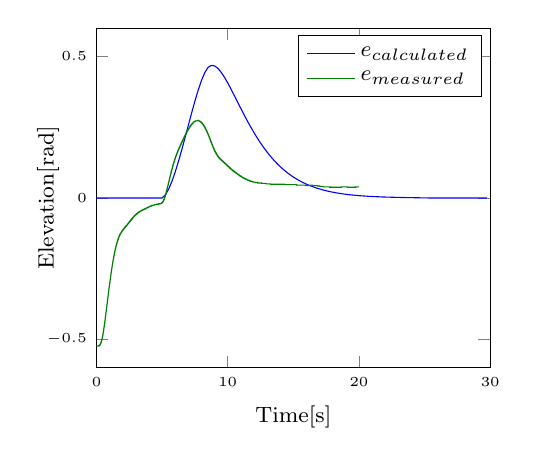
\begin{tikzpicture}

\begin{axis}[%
width = 5cm,
at={(0.758in,0.488in)},
scale only axis,
xmin=0,
xmax=30,
xlabel={\footnotesize{Time[s]}},
ymin=-0.6,
ymax=0.6,
ylabel={\footnotesize{Elevation[rad]}},
axis background/.style={fill=white},
ylabel shift = -0.4cm,
ticklabel style = {font=\tiny},
legend style={legend cell align=left, align=left, draw=black, font = \footnotesize}
]
\addplot [color=blue]
  table[row sep=crcr]{%
0	0\\
5	0\\
5.25	0.0111790084870798\\
5.5	0.0314285228123445\\
5.75	0.0589571543992378\\
6	0.0922242778688513\\
6.25	0.129875847906554\\
6.5	0.170685381629585\\
6.75	0.213497796741997\\
7.25	0.300541641256594\\
7.5	0.34232898323306\\
7.75	0.38111598941132\\
8	0.415265459007205\\
8.25	0.442852238150678\\
8.5	0.46158524270497\\
8.75	0.468715878925309\\
9	0.466851842459036\\
9.25	0.458129971010763\\
9.5	0.444293585959862\\
9.75	0.426757677384973\\
10	0.406662971231832\\
10.25	0.384923307218362\\
10.75	0.339254788123753\\
11.25	0.293847504952478\\
11.5	0.272037456697252\\
11.75	0.251088367331022\\
12	0.231125940976632\\
12.25	0.212230920522753\\
12.5	0.194448554601916\\
12.75	0.177795884159032\\
13	0.16226822316548\\
13.25	0.147844447077212\\
13.5	0.134491694237489\\
13.75	0.122167453715186\\
14	0.110823445674527\\
14.25	0.100407024401854\\
14.5	0.0908636264836069\\
14.75	0.0821376572517032\\
15	0.0741736887539624\\
15.25	0.0669178221019777\\
15.5	0.0603172853547704\\
15.75	0.0543215239931385\\
16	0.0488827401906597\\
16.25	0.0439552884880605\\
16.75	0.0354651938147548\\
17.25	0.0285412354643277\\
17.75	0.0229153425454278\\
18.25	0.0183591876706615\\
18.75	0.0146800138948002\\
19.25	0.0117162649150906\\
20	0.00832798453404848\\
20.75	0.00590001772599535\\
21.75	0.00370831938445448\\
23	0.00206173375537944\\
25.5	0\\
29.75	0\\
};
\addlegendentry{$e_{\text{calculated}}$}

\addplot [color=black!50!green]
  table[row sep=crcr]{%
0	-0.523598775598298\\
0.167999999999999	-0.523598775598298\\
0.170000000000002	-0.522064794810412\\
0.222000000000001	-0.522064794810412\\
0.224	-0.520530814022528\\
0.256	-0.520530814022528\\
0.257999999999999	-0.518996833234642\\
0.277999999999999	-0.518996833234642\\
0.280000000000001	-0.517462852446755\\
0.297999999999998	-0.517462852446755\\
0.300000000000001	-0.515928871658872\\
0.312000000000001	-0.515928871658872\\
0.314	-0.514394890870985\\
0.326000000000001	-0.514394890870985\\
0.327999999999999	-0.512860910083099\\
0.338000000000001	-0.512860910083099\\
0.34	-0.511326929295215\\
0.347999999999999	-0.511326929295215\\
0.350000000000001	-0.509792948507329\\
0.359999999999999	-0.509792948507329\\
0.361999999999998	-0.508258967719442\\
0.370000000000001	-0.508258967719442\\
0.372	-0.506724986931555\\
0.379999999999999	-0.506724986931555\\
0.382000000000001	-0.505191006143672\\
0.388000000000002	-0.505191006143672\\
0.390000000000001	-0.503657025355785\\
0.396000000000001	-0.503657025355785\\
0.398	-0.502123044567899\\
0.405999999999999	-0.502123044567899\\
0.408000000000001	-0.500589063780016\\
0.414000000000001	-0.500589063780016\\
0.416	-0.499055082992129\\
0.422000000000001	-0.499055082992129\\
0.423999999999999	-0.497521102204242\\
0.43	-0.497521102204242\\
0.431999999999999	-0.495987121416356\\
0.436	-0.495987121416356\\
0.437999999999999	-0.494453140628472\\
0.443999999999999	-0.494453140628472\\
0.446000000000002	-0.492919159840586\\
0.449999999999999	-0.492919159840586\\
0.452000000000002	-0.491385179052699\\
0.456	-0.491385179052699\\
0.457999999999998	-0.489851198264816\\
0.462	-0.489851198264816\\
0.463999999999999	-0.488317217476929\\
0.469999999999999	-0.488317217476929\\
0.472000000000001	-0.486783236689043\\
0.475999999999999	-0.486783236689043\\
0.478000000000002	-0.485249255901159\\
0.481999999999999	-0.485249255901159\\
0.484000000000002	-0.483715275113273\\
0.488	-0.483715275113273\\
0.489999999999998	-0.482181294325386\\
0.494	-0.482181294325386\\
0.495999999999999	-0.480647313537499\\
0.5	-0.480647313537499\\
0.501999999999999	-0.479113332749616\\
0.504000000000001	-0.479113332749616\\
0.506	-0.47757935196173\\
0.510000000000002	-0.47757935196173\\
0.512	-0.476045371173843\\
0.516000000000002	-0.476045371173843\\
0.518000000000001	-0.47451139038596\\
0.52	-0.47451139038596\\
0.521999999999998	-0.472977409598073\\
0.526	-0.472977409598073\\
0.527999999999999	-0.471443428810186\\
0.532	-0.471443428810186\\
0.533999999999999	-0.469909448022303\\
0.536000000000001	-0.469909448022303\\
0.538	-0.468375467234416\\
0.542000000000002	-0.468375467234416\\
0.544	-0.46684148644653\\
0.545999999999999	-0.46684148644653\\
0.548000000000002	-0.465307505658643\\
0.552	-0.465307505658643\\
0.553999999999998	-0.46377352487076\\
0.558	-0.46377352487076\\
0.559999999999999	-0.462239544082873\\
0.562000000000001	-0.462239544082873\\
0.564	-0.460705563294987\\
0.568000000000001	-0.460705563294987\\
0.57	-0.459171582507103\\
0.571999999999999	-0.459171582507103\\
0.574000000000002	-0.457637601719217\\
0.576000000000001	-0.457637601719217\\
0.577999999999999	-0.45610362093133\\
0.582000000000001	-0.45610362093133\\
0.584	-0.454569640143443\\
0.585999999999999	-0.454569640143443\\
0.588000000000001	-0.45303565935556\\
0.591999999999999	-0.45303565935556\\
0.594000000000001	-0.451501678567674\\
0.596	-0.451501678567674\\
0.597999999999999	-0.449967697779787\\
0.602	-0.449967697779787\\
0.603999999999999	-0.448433716991904\\
0.606000000000002	-0.448433716991904\\
0.608000000000001	-0.446899736204017\\
0.609999999999999	-0.446899736204017\\
0.611999999999998	-0.44536575541613\\
0.616	-0.44536575541613\\
0.617999999999999	-0.443831774628247\\
0.620000000000001	-0.443831774628247\\
0.622	-0.44229779384036\\
0.623999999999999	-0.44229779384036\\
0.626000000000001	-0.440763813052474\\
0.628	-0.440763813052474\\
0.629999999999999	-0.439229832264587\\
0.634	-0.439229832264587\\
0.635999999999999	-0.437695851476704\\
0.638000000000002	-0.437695851476704\\
0.640000000000001	-0.436161870688817\\
0.641999999999999	-0.436161870688817\\
0.643999999999998	-0.434627889900931\\
0.646000000000001	-0.434627889900931\\
0.648	-0.433093909113047\\
0.649999999999999	-0.433093909113047\\
0.652000000000001	-0.431559928325161\\
0.655999999999999	-0.431559928325161\\
0.658000000000001	-0.430025947537274\\
0.66	-0.430025947537274\\
0.661999999999999	-0.428491966749387\\
0.664000000000001	-0.428491966749387\\
0.666	-0.426957985961504\\
0.667999999999999	-0.426957985961504\\
0.670000000000002	-0.425424005173618\\
0.672000000000001	-0.425424005173618\\
0.673999999999999	-0.423890024385731\\
0.675999999999998	-0.423890024385731\\
0.678000000000001	-0.422356043597848\\
0.681999999999999	-0.422356043597848\\
0.684000000000001	-0.420822062809961\\
0.686	-0.420822062809961\\
0.687999999999999	-0.419288082022074\\
0.690000000000001	-0.419288082022074\\
0.692	-0.417754101234191\\
0.693999999999999	-0.417754101234191\\
0.696000000000002	-0.416220120446305\\
0.698	-0.416220120446305\\
0.699999999999999	-0.414686139658418\\
0.702000000000002	-0.414686139658418\\
0.704000000000001	-0.413152158870531\\
0.706	-0.413152158870531\\
0.707999999999998	-0.411618178082648\\
0.710000000000001	-0.411618178082648\\
0.712	-0.410084197294761\\
0.713999999999999	-0.410084197294761\\
0.716000000000001	-0.408550216506875\\
0.719999999999999	-0.408550216506875\\
0.722000000000001	-0.407016235718991\\
0.724	-0.407016235718991\\
0.725999999999999	-0.405482254931105\\
0.728000000000002	-0.405482254931105\\
0.73	-0.403948274143218\\
0.731999999999999	-0.403948274143218\\
0.734000000000002	-0.402414293355335\\
0.736000000000001	-0.402414293355335\\
0.738	-0.400880312567448\\
0.739999999999998	-0.400880312567448\\
0.742000000000001	-0.399346331779562\\
0.744	-0.399346331779562\\
0.745999999999999	-0.397812350991675\\
0.748000000000001	-0.397812350991675\\
0.75	-0.396278370203792\\
0.751999999999999	-0.396278370203792\\
0.754000000000001	-0.394744389415905\\
0.756	-0.394744389415905\\
0.757999999999999	-0.393210408628018\\
0.760000000000002	-0.393210408628018\\
0.762	-0.391676427840135\\
0.763999999999999	-0.391676427840135\\
0.766000000000002	-0.390142447052249\\
0.768000000000001	-0.390142447052249\\
0.77	-0.388608466264362\\
0.774000000000001	-0.388608466264362\\
0.776	-0.387074485476475\\
0.777999999999999	-0.387074485476475\\
0.780000000000001	-0.385540504688592\\
0.782	-0.385540504688592\\
0.783999999999999	-0.384006523900705\\
0.786000000000001	-0.384006523900705\\
0.788	-0.382472543112819\\
0.789999999999999	-0.382472543112819\\
0.792000000000002	-0.380938562324936\\
0.794	-0.380938562324936\\
0.795999999999999	-0.379404581537049\\
0.798000000000002	-0.379404581537049\\
0.800000000000001	-0.377870600749162\\
0.802	-0.377870600749162\\
0.803999999999998	-0.376336619961279\\
0.806000000000001	-0.376336619961279\\
0.808	-0.374802639173392\\
0.809999999999999	-0.374802639173392\\
0.812000000000001	-0.373268658385506\\
0.814	-0.373268658385506\\
0.815999999999999	-0.371734677597619\\
0.818000000000001	-0.371734677597619\\
0.82	-0.370200696809736\\
0.821999999999999	-0.370200696809736\\
0.824000000000002	-0.368666716021849\\
0.826000000000001	-0.368666716021849\\
0.827999999999999	-0.367132735233962\\
0.830000000000002	-0.367132735233962\\
0.832000000000001	-0.365598754446079\\
0.834	-0.365598754446079\\
0.835999999999999	-0.364064773658193\\
0.838000000000001	-0.364064773658193\\
0.84	-0.362530792870306\\
0.841999999999999	-0.362530792870306\\
0.844000000000001	-0.360996812082419\\
0.846	-0.360996812082419\\
0.847999999999999	-0.359462831294536\\
0.850000000000001	-0.359462831294536\\
0.852	-0.357928850506649\\
0.853999999999999	-0.357928850506649\\
0.856000000000002	-0.356394869718763\\
0.858000000000001	-0.356394869718763\\
0.859999999999999	-0.35486088893088\\
0.864000000000001	-0.35486088893088\\
0.866	-0.353326908142993\\
0.867999999999999	-0.353326908142993\\
0.870000000000001	-0.351792927355106\\
0.872	-0.351792927355106\\
0.873999999999999	-0.350258946567223\\
0.876000000000001	-0.350258946567223\\
0.878	-0.348724965779336\\
0.879999999999999	-0.348724965779336\\
0.882000000000001	-0.34719098499145\\
0.884	-0.34719098499145\\
0.885999999999999	-0.345657004203563\\
0.888000000000002	-0.345657004203563\\
0.890000000000001	-0.34412302341568\\
0.891999999999999	-0.34412302341568\\
0.893999999999998	-0.342589042627793\\
0.896000000000001	-0.342589042627793\\
0.898	-0.341055061839906\\
0.899999999999999	-0.341055061839906\\
0.902000000000001	-0.339521081052023\\
0.904	-0.339521081052023\\
0.905999999999999	-0.337987100264137\\
0.908000000000001	-0.337987100264137\\
0.91	-0.33645311947625\\
0.911999999999999	-0.33645311947625\\
0.914000000000001	-0.334919138688367\\
0.916	-0.334919138688367\\
0.917999999999999	-0.33338515790048\\
0.920000000000002	-0.33338515790048\\
0.922000000000001	-0.331851177112593\\
0.923999999999999	-0.331851177112593\\
0.925999999999998	-0.330317196324707\\
0.93	-0.330317196324707\\
0.931999999999999	-0.328783215536824\\
0.934000000000001	-0.328783215536824\\
0.936	-0.327249234748937\\
0.937999999999999	-0.327249234748937\\
0.940000000000001	-0.32571525396105\\
0.942	-0.32571525396105\\
0.943999999999999	-0.324181273173167\\
0.946000000000002	-0.324181273173167\\
0.948	-0.32264729238528\\
0.949999999999999	-0.32264729238528\\
0.952000000000002	-0.321113311597394\\
0.954000000000001	-0.321113311597394\\
0.956	-0.319579330809507\\
0.957999999999998	-0.319579330809507\\
0.960000000000001	-0.318045350021624\\
0.962	-0.318045350021624\\
0.963999999999999	-0.316511369233737\\
0.968	-0.316511369233737\\
0.969999999999999	-0.31497738844585\\
0.972000000000001	-0.31497738844585\\
0.974	-0.313443407657967\\
0.975999999999999	-0.313443407657967\\
0.978000000000002	-0.311909426870081\\
0.98	-0.311909426870081\\
0.981999999999999	-0.310375446082194\\
0.984000000000002	-0.310375446082194\\
0.986000000000001	-0.308841465294311\\
0.989999999999998	-0.308841465294311\\
0.992000000000001	-0.307307484506424\\
0.994	-0.307307484506424\\
0.995999999999999	-0.305773503718537\\
0.998000000000001	-0.305773503718537\\
1	-0.304239522930651\\
1.002	-0.304239522930651\\
1.004	-0.302705542142768\\
1.006	-0.302705542142768\\
1.008	-0.301171561354881\\
1.01	-0.301171561354881\\
1.012	-0.299637580566994\\
1.016	-0.299637580566994\\
1.018	-0.298103599779111\\
1.02	-0.298103599779111\\
1.022	-0.296569618991224\\
1.024	-0.296569618991224\\
1.026	-0.295035638203338\\
1.028	-0.295035638203338\\
1.03	-0.293501657415451\\
1.032	-0.293501657415451\\
1.034	-0.291967676627568\\
1.038	-0.291967676627568\\
1.04	-0.290433695839681\\
1.042	-0.290433695839681\\
1.044	-0.288899715051794\\
1.046	-0.288899715051794\\
1.048	-0.287365734263911\\
1.05	-0.287365734263911\\
1.052	-0.285831753476025\\
1.056	-0.285831753476025\\
1.058	-0.284297772688138\\
1.06	-0.284297772688138\\
1.062	-0.282763791900255\\
1.064	-0.282763791900255\\
1.066	-0.281229811112368\\
1.068	-0.281229811112368\\
1.07	-0.279695830324481\\
1.074	-0.279695830324481\\
1.076	-0.278161849536595\\
1.078	-0.278161849536595\\
1.08	-0.276627868748712\\
1.082	-0.276627868748712\\
1.084	-0.275093887960825\\
1.088	-0.275093887960825\\
1.09	-0.273559907172938\\
1.092	-0.273559907172938\\
1.094	-0.272025926385055\\
1.096	-0.272025926385055\\
1.098	-0.270491945597168\\
1.102	-0.270491945597168\\
1.104	-0.268957964809282\\
1.106	-0.268957964809282\\
1.108	-0.267423984021399\\
1.112	-0.267423984021399\\
1.114	-0.265890003233512\\
1.116	-0.265890003233512\\
1.118	-0.264356022445625\\
1.12	-0.264356022445625\\
1.122	-0.262822041657738\\
1.126	-0.262822041657738\\
1.128	-0.261288060869855\\
1.13	-0.261288060869855\\
1.132	-0.259754080081969\\
1.136	-0.259754080081969\\
1.138	-0.258220099294082\\
1.14	-0.258220099294082\\
1.142	-0.256686118506199\\
1.146	-0.256686118506199\\
1.148	-0.255152137718312\\
1.15	-0.255152137718312\\
1.152	-0.253618156930425\\
1.156	-0.253618156930425\\
1.158	-0.252084176142539\\
1.16	-0.252084176142539\\
1.162	-0.250550195354656\\
1.166	-0.250550195354656\\
1.168	-0.249016214566769\\
1.17	-0.249016214566769\\
1.172	-0.247482233778882\\
1.176	-0.247482233778882\\
1.178	-0.245948252990999\\
1.18	-0.245948252990999\\
1.182	-0.244414272203112\\
1.186	-0.244414272203112\\
1.188	-0.242880291415226\\
1.19	-0.242880291415226\\
1.192	-0.241346310627343\\
1.196	-0.241346310627343\\
1.198	-0.239812329839456\\
1.2	-0.239812329839456\\
1.202	-0.238278349051569\\
1.206	-0.238278349051569\\
1.208	-0.236744368263683\\
1.212	-0.236744368263683\\
1.214	-0.235210387475799\\
1.216	-0.235210387475799\\
1.218	-0.233676406687913\\
1.222	-0.233676406687913\\
1.224	-0.232142425900026\\
1.228	-0.232142425900026\\
1.23	-0.230608445112143\\
1.232	-0.230608445112143\\
1.234	-0.229074464324256\\
1.238	-0.229074464324256\\
1.24	-0.227540483536369\\
1.244	-0.227540483536369\\
1.246	-0.226006502748483\\
1.25	-0.226006502748483\\
1.252	-0.2244725219606\\
1.256	-0.2244725219606\\
1.258	-0.222938541172713\\
1.262	-0.222938541172713\\
1.264	-0.221404560384826\\
1.266	-0.221404560384826\\
1.268	-0.219870579596943\\
1.272	-0.219870579596943\\
1.274	-0.218336598809056\\
1.278	-0.218336598809056\\
1.28	-0.21680261802117\\
1.284	-0.21680261802117\\
1.286	-0.215268637233287\\
1.29	-0.215268637233287\\
1.292	-0.2137346564454\\
1.296	-0.2137346564454\\
1.298	-0.212200675657513\\
1.302	-0.212200675657513\\
1.304	-0.210666694869627\\
1.308	-0.210666694869627\\
1.31	-0.209132714081743\\
1.314	-0.209132714081743\\
1.316	-0.207598733293857\\
1.32	-0.207598733293857\\
1.322	-0.20606475250597\\
1.326	-0.20606475250597\\
1.328	-0.204530771718087\\
1.334	-0.204530771718087\\
1.336	-0.2029967909302\\
1.338	-0.2029967909302\\
1.34	-0.201462810142313\\
1.346	-0.201462810142313\\
1.348	-0.19992882935443\\
1.352	-0.19992882935443\\
1.354	-0.198394848566544\\
1.358	-0.198394848566544\\
1.36	-0.196860867778657\\
1.364	-0.196860867778657\\
1.366	-0.19532688699077\\
1.372	-0.19532688699077\\
1.374	-0.193792906202887\\
1.378	-0.193792906202887\\
1.38	-0.192258925415\\
1.386	-0.192258925415\\
1.388	-0.190724944627114\\
1.392	-0.190724944627114\\
1.394	-0.189190963839231\\
1.4	-0.189190963839231\\
1.402	-0.187656983051344\\
1.406	-0.187656983051344\\
1.408	-0.186123002263457\\
1.414	-0.186123002263457\\
1.416	-0.184589021475571\\
1.422	-0.184589021475571\\
1.424	-0.183055040687687\\
1.43	-0.183055040687687\\
1.432	-0.181521059899801\\
1.436	-0.181521059899801\\
1.438	-0.179987079111914\\
1.444	-0.179987079111914\\
1.446	-0.178453098324031\\
1.452	-0.178453098324031\\
1.454	-0.176919117536144\\
1.46	-0.176919117536144\\
1.462	-0.175385136748258\\
1.468	-0.175385136748258\\
1.47	-0.173851155960374\\
1.474	-0.173851155960374\\
1.476	-0.172317175172488\\
1.484	-0.172317175172488\\
1.486	-0.170783194384601\\
1.492	-0.170783194384601\\
1.494	-0.169249213596714\\
1.5	-0.169249213596714\\
1.502	-0.167715232808831\\
1.508	-0.167715232808831\\
1.51	-0.166181252020944\\
1.516	-0.166181252020944\\
1.518	-0.164647271233058\\
1.526	-0.164647271233058\\
1.528	-0.163113290445175\\
1.536	-0.163113290445175\\
1.538	-0.161579309657288\\
1.546	-0.161579309657288\\
1.548	-0.160045328869401\\
1.554	-0.160045328869401\\
1.556	-0.158511348081515\\
1.564	-0.158511348081515\\
1.566	-0.156977367293631\\
1.574	-0.156977367293631\\
1.576	-0.155443386505745\\
1.584	-0.155443386505745\\
1.586	-0.153909405717858\\
1.594	-0.153909405717858\\
1.596	-0.152375424929975\\
1.604	-0.152375424929975\\
1.606	-0.150841444142088\\
1.616	-0.150841444142088\\
1.618	-0.149307463354202\\
1.626	-0.149307463354202\\
1.628	-0.147773482566318\\
1.638	-0.147773482566318\\
1.64	-0.146239501778432\\
1.648	-0.146239501778432\\
1.65	-0.144705520990545\\
1.66	-0.144705520990545\\
1.662	-0.143171540202658\\
1.672	-0.143171540202658\\
1.674	-0.141637559414775\\
1.684	-0.141637559414775\\
1.686	-0.140103578626888\\
1.7	-0.140103578626888\\
1.702	-0.138569597839002\\
1.712	-0.138569597839002\\
1.714	-0.137035617051119\\
1.726	-0.137035617051119\\
1.728	-0.135501636263232\\
1.74	-0.135501636263232\\
1.742	-0.133967655475345\\
1.754	-0.133967655475345\\
1.756	-0.132433674687462\\
1.768	-0.132433674687462\\
1.77	-0.130899693899575\\
1.784	-0.130899693899575\\
1.786	-0.129365713111689\\
1.8	-0.129365713111689\\
1.802	-0.127831732323802\\
1.816	-0.127831732323802\\
1.818	-0.126297751535919\\
1.836	-0.126297751535919\\
1.838	-0.124763770748032\\
1.856	-0.124763770748032\\
1.858	-0.123229789960146\\
1.874	-0.123229789960146\\
1.876	-0.121695809172262\\
1.892	-0.121695809172262\\
1.894	-0.120161828384376\\
1.912	-0.120161828384376\\
1.914	-0.118627847596489\\
1.934	-0.118627847596489\\
1.936	-0.117093866808602\\
1.956	-0.117093866808602\\
1.958	-0.115559886020719\\
1.98	-0.115559886020719\\
1.982	-0.114025905232833\\
2.004	-0.114025905232833\\
2.006	-0.112491924444946\\
2.028	-0.112491924444946\\
2.03	-0.110957943657063\\
2.056	-0.110957943657063\\
2.058	-0.109423962869176\\
2.08	-0.109423962869176\\
2.082	-0.107889982081289\\
2.108	-0.107889982081289\\
2.11	-0.106356001293406\\
2.138	-0.106356001293406\\
2.14	-0.104822020505519\\
2.168	-0.104822020505519\\
2.17	-0.103288039717633\\
2.19	-0.103288039717633\\
2.192	-0.101754058929746\\
2.218	-0.101754058929746\\
2.22	-0.100220078141863\\
2.248	-0.100220078141863\\
2.25	-0.0986860973539763\\
2.278	-0.0986860973539763\\
2.28	-0.0971521165660896\\
2.308	-0.0971521165660896\\
2.31	-0.0956181357782064\\
2.33	-0.0956181357782064\\
2.332	-0.0940841549903197\\
2.36	-0.0940841549903197\\
2.362	-0.0925501742024331\\
2.388	-0.0925501742024331\\
2.39	-0.0910161934145464\\
2.414	-0.0910161934145464\\
2.416	-0.0894822126266632\\
2.442	-0.0894822126266632\\
2.444	-0.0879482318387765\\
2.47	-0.0879482318387765\\
2.472	-0.0864142510508898\\
2.494	-0.0864142510508898\\
2.496	-0.0848802702630067\\
2.522	-0.0848802702630067\\
2.524	-0.08334628947512\\
2.548	-0.08334628947512\\
2.55	-0.0818123086872333\\
2.572	-0.0818123086872333\\
2.574	-0.0802783278993502\\
2.6	-0.0802783278993502\\
2.602	-0.0787443471114635\\
2.628	-0.0787443471114635\\
2.63	-0.0772103663235768\\
2.65	-0.0772103663235768\\
2.652	-0.0756763855356901\\
2.678	-0.0756763855356901\\
2.68	-0.074142404747807\\
2.706	-0.074142404747807\\
2.708	-0.0726084239599203\\
2.734	-0.0726084239599203\\
2.736	-0.0710744431720336\\
2.762	-0.0710744431720336\\
2.764	-0.0695404623841505\\
2.79	-0.0695404623841505\\
2.792	-0.0680064815962638\\
2.816	-0.0680064815962638\\
2.818	-0.0664725008083771\\
2.848	-0.0664725008083771\\
2.85	-0.0649385200204904\\
2.88	-0.0649385200204904\\
2.882	-0.0634045392326072\\
2.914	-0.0634045392326072\\
2.916	-0.0618705584447206\\
2.944	-0.0618705584447206\\
2.946	-0.0603365776568339\\
2.98	-0.0603365776568339\\
2.982	-0.0588025968689507\\
3.016	-0.0588025968689507\\
3.018	-0.057268616081064\\
3.054	-0.057268616081064\\
3.056	-0.0557346352931773\\
3.092	-0.0557346352931773\\
3.094	-0.0542006545052942\\
3.136	-0.0542006545052942\\
3.138	-0.0526666737174075\\
3.178	-0.0526666737174075\\
3.18	-0.0511326929295208\\
3.228	-0.0511326929295208\\
3.23	-0.0495987121416341\\
3.274	-0.0495987121416341\\
3.276	-0.048064731353751\\
3.324	-0.048064731353751\\
3.326	-0.0465307505658643\\
3.392	-0.0465307505658643\\
3.394	-0.0449967697779776\\
3.444	-0.0449967697779776\\
3.446	-0.0434627889900945\\
3.514	-0.0434627889900945\\
3.516	-0.0419288082022078\\
3.576	-0.0419288082022078\\
3.578	-0.0403948274143211\\
3.646	-0.0403948274143211\\
3.648	-0.038860846626438\\
3.716	-0.038860846626438\\
3.718	-0.0373268658385513\\
3.786	-0.0373268658385513\\
3.788	-0.0357928850506646\\
3.846	-0.0357928850506646\\
3.848	-0.0342589042627779\\
3.916	-0.0342589042627779\\
3.918	-0.0327249234748948\\
3.978	-0.0327249234748948\\
3.98	-0.0311909426870081\\
4.05	-0.0311909426870081\\
4.052	-0.0296569618991214\\
4.128	-0.0296569618991214\\
4.13	-0.0281229811112382\\
4.208	-0.0281229811112382\\
4.21	-0.0265890003233515\\
4.314	-0.0265890003233515\\
4.316	-0.0250550195354649\\
4.426	-0.0250550195354649\\
4.428	-0.0235210387475782\\
4.564	-0.0235210387475782\\
4.566	-0.021987057959695\\
4.732	-0.021987057959695\\
4.734	-0.0204530771718083\\
4.89	-0.0204530771718083\\
4.892	-0.0189190963839216\\
4.96	-0.0189190963839216\\
4.962	-0.0173851155960385\\
4.994	-0.0173851155960385\\
4.996	-0.0158511348081518\\
5.024	-0.0158511348081518\\
5.026	-0.0143171540202651\\
5.05	-0.0143171540202651\\
5.052	-0.012783173232382\\
5.072	-0.012783173232382\\
5.074	-0.0112491924444953\\
5.09	-0.0112491924444953\\
5.092	-0.0097152116566086\\
5.106	-0.0097152116566086\\
5.108	-0.00818123086872191\\
5.12	-0.00818123086872191\\
5.122	-0.00664725008083877\\
5.134	-0.00664725008083877\\
5.136	-0.00511326929295208\\
5.148	-0.00511326929295208\\
5.15	-0.00357928850506539\\
5.162	-0.00357928850506539\\
5.164	-0.00204530771718225\\
5.174	-0.00204530771718225\\
5.176	-0.000511326929295564\\
5.186	-0.000511326929295564\\
5.188	0.00102265385859113\\
5.198	0.00102265385859113\\
5.2	0.00255663464647782\\
5.208	0.00255663464647782\\
5.21	0.00409061543436096\\
5.22	0.00409061543436096\\
5.222	0.00562459622224765\\
5.23	0.00562459622224765\\
5.232	0.00715857701013434\\
5.24	0.00715857701013434\\
5.242	0.00869255779801748\\
5.25	0.00869255779801748\\
5.252	0.0102265385859042\\
5.26	0.0102265385859042\\
5.262	0.0117605193737909\\
5.27	0.0117605193737909\\
5.272	0.013294500161674\\
5.278	0.013294500161674\\
5.28	0.0148284809495607\\
5.288	0.0148284809495607\\
5.29	0.0163624617374474\\
5.298	0.0163624617374474\\
5.3	0.0178964425253341\\
5.306	0.0178964425253341\\
5.308	0.0194304233132172\\
5.316	0.0194304233132172\\
5.318	0.0209644041011039\\
5.324	0.0209644041011039\\
5.326	0.0224983848889906\\
5.332	0.0224983848889906\\
5.334	0.0240323656768737\\
5.342	0.0240323656768737\\
5.344	0.0255663464647604\\
5.35	0.0255663464647604\\
5.352	0.0271003272526471\\
5.358	0.0271003272526471\\
5.36	0.0286343080405302\\
5.366	0.0286343080405302\\
5.368	0.0301682888284169\\
5.374	0.0301682888284169\\
5.376	0.0317022696163036\\
5.384	0.0317022696163036\\
5.386	0.0332362504041903\\
5.392	0.0332362504041903\\
5.394	0.0347702311920735\\
5.4	0.0347702311920735\\
5.402	0.0363042119799601\\
5.408	0.0363042119799601\\
5.41	0.0378381927678468\\
5.416	0.0378381927678468\\
5.418	0.03937217355573\\
5.424	0.03937217355573\\
5.426	0.0409061543436167\\
5.432	0.0409061543436167\\
5.434	0.0424401351315034\\
5.44	0.0424401351315034\\
5.442	0.04397411591939\\
5.448	0.04397411591939\\
5.45	0.0455080967072732\\
5.456	0.0455080967072732\\
5.458	0.0470420774951599\\
5.464	0.0470420774951599\\
5.466	0.0485760582830466\\
5.472	0.0485760582830466\\
5.474	0.0501100390709297\\
5.48	0.0501100390709297\\
5.482	0.0516440198588164\\
5.488	0.0516440198588164\\
5.49	0.0531780006467031\\
5.494	0.0531780006467031\\
5.496	0.0547119814345862\\
5.502	0.0547119814345862\\
5.504	0.0562459622224729\\
5.512	0.0562459622224729\\
5.514	0.0577799430103596\\
5.518	0.0577799430103596\\
5.52	0.0593139237982463\\
5.528	0.0593139237982463\\
5.53	0.0608479045861294\\
5.534	0.0608479045861294\\
5.536	0.0623818853740161\\
5.542	0.0623818853740161\\
5.544	0.0639158661619028\\
5.55	0.0639158661619028\\
5.552	0.065449846949786\\
5.558	0.065449846949786\\
5.56	0.0669838277376726\\
5.566	0.0669838277376726\\
5.568	0.0685178085255593\\
5.574	0.0685178085255593\\
5.576	0.070051789313446\\
5.582	0.070051789313446\\
5.584	0.0715857701013292\\
5.59	0.0715857701013292\\
5.592	0.0731197508892159\\
5.598	0.0731197508892159\\
5.6	0.0746537316771025\\
5.608	0.0746537316771025\\
5.61	0.0761877124649857\\
5.614	0.0761877124649857\\
5.616	0.0777216932528724\\
5.624	0.0777216932528724\\
5.626	0.0792556740407591\\
5.632	0.0792556740407591\\
5.634	0.0807896548286422\\
5.638	0.0807896548286422\\
5.64	0.0823236356165289\\
5.648	0.0823236356165289\\
5.65	0.0838576164044156\\
5.656	0.0838576164044156\\
5.658	0.0853915971923023\\
5.664	0.0853915971923023\\
5.666	0.0869255779801854\\
5.672	0.0869255779801854\\
5.674	0.0884595587680721\\
5.68	0.0884595587680721\\
5.682	0.0899935395559588\\
5.69	0.0899935395559588\\
5.692	0.0915275203438419\\
5.696	0.0915275203438419\\
5.698	0.0930615011317286\\
5.706	0.0930615011317286\\
5.708	0.0945954819196153\\
5.714	0.0945954819196153\\
5.716	0.0961294627074984\\
5.722	0.0961294627074984\\
5.724	0.0976634434953851\\
5.732	0.0976634434953851\\
5.734	0.0991974242832718\\
5.74	0.0991974242832718\\
5.742	0.100731405071159\\
5.75	0.100731405071159\\
5.752	0.102265385859042\\
5.758	0.102265385859042\\
5.76	0.103799366646928\\
5.768	0.103799366646928\\
5.77	0.105333347434815\\
5.776	0.105333347434815\\
5.778	0.106867328222698\\
5.784	0.106867328222698\\
5.786	0.108401309010585\\
5.794	0.108401309010585\\
5.796	0.109935289798472\\
5.802	0.109935289798472\\
5.804	0.111469270586358\\
5.812	0.111469270586358\\
5.814	0.113003251374241\\
5.822	0.113003251374241\\
5.824	0.114537232162128\\
5.83	0.114537232162128\\
5.832	0.116071212950015\\
5.84	0.116071212950015\\
5.842	0.117605193737898\\
5.85	0.117605193737898\\
5.852	0.119139174525785\\
5.86	0.119139174525785\\
5.862	0.120673155313671\\
5.87	0.120673155313671\\
5.872	0.122207136101554\\
5.88	0.122207136101554\\
5.882	0.123741116889441\\
5.89	0.123741116889441\\
5.892	0.125275097677328\\
5.9	0.125275097677328\\
5.902	0.126809078465214\\
5.91	0.126809078465214\\
5.912	0.128343059253098\\
5.92	0.128343059253098\\
5.922	0.129877040040984\\
5.93	0.129877040040984\\
5.932	0.131411020828871\\
5.94	0.131411020828871\\
5.942	0.132945001616754\\
5.952	0.132945001616754\\
5.954	0.134478982404641\\
5.962	0.134478982404641\\
5.964	0.136012963192528\\
5.972	0.136012963192528\\
5.974	0.137546943980414\\
5.984	0.137546943980414\\
5.986	0.139080924768297\\
5.996	0.139080924768297\\
5.998	0.140614905556184\\
6.006	0.140614905556184\\
6.008	0.142148886344071\\
6.018	0.142148886344071\\
6.02	0.143682867131954\\
6.028	0.143682867131954\\
6.03	0.145216847919841\\
6.04	0.145216847919841\\
6.042	0.146750828707727\\
6.05	0.146750828707727\\
6.052	0.14828480949561\\
6.064	0.14828480949561\\
6.066	0.149818790283497\\
6.076	0.149818790283497\\
6.078	0.151352771071384\\
6.088	0.151352771071384\\
6.09	0.15288675185927\\
6.1	0.15288675185927\\
6.102	0.154420732647154\\
6.114	0.154420732647154\\
6.116	0.15595471343504\\
6.126	0.15595471343504\\
6.128	0.157488694222927\\
6.138	0.157488694222927\\
6.14	0.15902267501081\\
6.15	0.15902267501081\\
6.152	0.160556655798697\\
6.162	0.160556655798697\\
6.164	0.162090636586584\\
6.176	0.162090636586584\\
6.178	0.163624617374467\\
6.19	0.163624617374467\\
6.192	0.165158598162353\\
6.202	0.165158598162353\\
6.204	0.16669257895024\\
6.218	0.16669257895024\\
6.22	0.168226559738127\\
6.234	0.168226559738127\\
6.236	0.16976054052601\\
6.248	0.16976054052601\\
6.25	0.171294521313897\\
6.262	0.171294521313897\\
6.264	0.172828502101783\\
6.276	0.172828502101783\\
6.278	0.174362482889666\\
6.29	0.174362482889666\\
6.292	0.175896463677553\\
6.304	0.175896463677553\\
6.306	0.17743044446544\\
6.318	0.17743044446544\\
6.32	0.178964425253326\\
6.332	0.178964425253326\\
6.334	0.18049840604121\\
6.348	0.18049840604121\\
6.35	0.182032386829096\\
6.366	0.182032386829096\\
6.368	0.183566367616983\\
6.38	0.183566367616983\\
6.382	0.185100348404866\\
6.396	0.185100348404866\\
6.398	0.186634329192753\\
6.41	0.186634329192753\\
6.412	0.188168309980639\\
6.424	0.188168309980639\\
6.426	0.189702290768523\\
6.438	0.189702290768523\\
6.44	0.191236271556409\\
6.454	0.191236271556409\\
6.456	0.192770252344296\\
6.47	0.192770252344296\\
6.472	0.194304233132183\\
6.486	0.194304233132183\\
6.488	0.195838213920066\\
6.5	0.195838213920066\\
6.502	0.197372194707953\\
6.516	0.197372194707953\\
6.518	0.198906175495839\\
6.532	0.198906175495839\\
6.534	0.200440156283722\\
6.546	0.200440156283722\\
6.548	0.201974137071609\\
6.56	0.201974137071609\\
6.562	0.203508117859496\\
6.576	0.203508117859496\\
6.578	0.205042098647382\\
6.592	0.205042098647382\\
6.594	0.206576079435266\\
6.608	0.206576079435266\\
6.61	0.208110060223152\\
6.624	0.208110060223152\\
6.626	0.209644041011039\\
6.64	0.209644041011039\\
6.642	0.211178021798922\\
6.656	0.211178021798922\\
6.658	0.212712002586809\\
6.67	0.212712002586809\\
6.672	0.214245983374695\\
6.684	0.214245983374695\\
6.686	0.215779964162579\\
6.7	0.215779964162579\\
6.702	0.217313944950465\\
6.716	0.217313944950465\\
6.718	0.218847925738352\\
6.734	0.218847925738352\\
6.736	0.220381906526239\\
6.75	0.220381906526239\\
6.752	0.221915887314122\\
6.768	0.221915887314122\\
6.77	0.223449868102009\\
6.784	0.223449868102009\\
6.786	0.224983848889895\\
6.8	0.224983848889895\\
6.802	0.226517829677778\\
6.816	0.226517829677778\\
6.818	0.228051810465665\\
6.832	0.228051810465665\\
6.834	0.229585791253552\\
6.848	0.229585791253552\\
6.85	0.231119772041435\\
6.868	0.231119772041435\\
6.87	0.232653752829322\\
6.884	0.232653752829322\\
6.886	0.234187733617208\\
6.904	0.234187733617208\\
6.906	0.235721714405095\\
6.92	0.235721714405095\\
6.922	0.237255695192978\\
6.938	0.237255695192978\\
6.94	0.238789675980865\\
6.956	0.238789675980865\\
6.958	0.240323656768751\\
6.974	0.240323656768751\\
6.976	0.241857637556635\\
6.994	0.241857637556635\\
6.996	0.243391618344521\\
7.016	0.243391618344521\\
7.018	0.244925599132408\\
7.034	0.244925599132408\\
7.036	0.246459579920295\\
7.056	0.246459579920295\\
7.058	0.247993560708178\\
7.074	0.247993560708178\\
7.076	0.249527541496064\\
7.096	0.249527541496064\\
7.098	0.251061522283951\\
7.118	0.251061522283951\\
7.12	0.252595503071834\\
7.142	0.252595503071834\\
7.144	0.254129483859721\\
7.166	0.254129483859721\\
7.168	0.255663464647608\\
7.19	0.255663464647608\\
7.192	0.257197445435491\\
7.212	0.257197445435491\\
7.214	0.258731426223378\\
7.238	0.258731426223378\\
7.24	0.260265407011264\\
7.266	0.260265407011264\\
7.268	0.261799387799151\\
7.298	0.261799387799151\\
7.3	0.263333368587034\\
7.324	0.263333368587034\\
7.326	0.264867349374921\\
7.358	0.264867349374921\\
7.36	0.266401330162807\\
7.388	0.266401330162807\\
7.39	0.267935310950691\\
7.436	0.267935310950691\\
7.438	0.269469291738577\\
7.484	0.269469291738577\\
7.486	0.271003272526464\\
7.534	0.271003272526464\\
7.536	0.272537253314351\\
7.542	0.272537253314351\\
7.544	0.271003272526464\\
7.546	0.272537253314351\\
7.664	0.272537253314351\\
7.666	0.274071234102234\\
7.67	0.274071234102234\\
7.672	0.272537253314351\\
7.676	0.272537253314351\\
7.678	0.274071234102234\\
7.682	0.274071234102234\\
7.684	0.272537253314351\\
7.686	0.272537253314351\\
7.688	0.274071234102234\\
7.694	0.274071234102234\\
7.696	0.272537253314351\\
7.698	0.272537253314351\\
7.7	0.274071234102234\\
7.708	0.274071234102234\\
7.71	0.272537253314351\\
7.712	0.274071234102234\\
7.756	0.274071234102234\\
7.758	0.272537253314351\\
7.76	0.274071234102234\\
7.766	0.274071234102234\\
7.768	0.272537253314351\\
7.772	0.272537253314351\\
7.774	0.274071234102234\\
7.778	0.274071234102234\\
7.78	0.272537253314351\\
7.858	0.272537253314351\\
7.86	0.271003272526464\\
7.918	0.271003272526464\\
7.92	0.269469291738577\\
7.954	0.269469291738577\\
7.956	0.267935310950691\\
7.962	0.267935310950691\\
7.964	0.269469291738577\\
7.966	0.267935310950691\\
7.98	0.267935310950691\\
7.982	0.266401330162807\\
7.984	0.266401330162807\\
7.986	0.267935310950691\\
7.99	0.267935310950691\\
7.992	0.266401330162807\\
8.016	0.266401330162807\\
8.018	0.264867349374921\\
8.02	0.264867349374921\\
8.022	0.266401330162807\\
8.026	0.266401330162807\\
8.028	0.264867349374921\\
8.05	0.264867349374921\\
8.052	0.263333368587034\\
8.076	0.263333368587034\\
8.078	0.261799387799151\\
8.08	0.261799387799151\\
8.082	0.263333368587034\\
8.086	0.263333368587034\\
8.088	0.261799387799151\\
8.11	0.261799387799151\\
8.112	0.260265407011264\\
8.132	0.260265407011264\\
8.134	0.258731426223378\\
8.154	0.258731426223378\\
8.156	0.257197445435491\\
8.17	0.257197445435491\\
8.172	0.255663464647608\\
8.192	0.255663464647608\\
8.194	0.254129483859721\\
8.214	0.254129483859721\\
8.216	0.252595503071834\\
8.23	0.252595503071834\\
8.232	0.251061522283951\\
8.252	0.251061522283951\\
8.254	0.249527541496064\\
8.266	0.249527541496064\\
8.268	0.247993560708178\\
8.286	0.247993560708178\\
8.288	0.246459579920295\\
8.3	0.246459579920295\\
8.302	0.244925599132408\\
8.314	0.244925599132408\\
8.316	0.243391618344521\\
8.336	0.243391618344521\\
8.338	0.241857637556635\\
8.35	0.241857637556635\\
8.352	0.240323656768751\\
8.368	0.240323656768751\\
8.37	0.238789675980865\\
8.384	0.238789675980865\\
8.386	0.237255695192978\\
8.4	0.237255695192978\\
8.402	0.235721714405095\\
8.414	0.235721714405095\\
8.416	0.234187733617208\\
8.428	0.234187733617208\\
8.43	0.232653752829322\\
8.442	0.232653752829322\\
8.444	0.231119772041435\\
8.456	0.231119772041435\\
8.458	0.229585791253552\\
8.47	0.229585791253552\\
8.472	0.228051810465665\\
8.486	0.228051810465665\\
8.488	0.226517829677778\\
8.5	0.226517829677778\\
8.502	0.224983848889895\\
8.514	0.224983848889895\\
8.516	0.223449868102009\\
8.528	0.223449868102009\\
8.53	0.221915887314122\\
8.542	0.221915887314122\\
8.544	0.220381906526239\\
8.556	0.220381906526239\\
8.558	0.218847925738352\\
8.57	0.218847925738352\\
8.572	0.217313944950465\\
8.582	0.217313944950465\\
8.584	0.215779964162579\\
8.594	0.215779964162579\\
8.596	0.214245983374695\\
8.608	0.214245983374695\\
8.61	0.212712002586809\\
8.62	0.212712002586809\\
8.622	0.211178021798922\\
8.632	0.211178021798922\\
8.634	0.209644041011039\\
8.646	0.209644041011039\\
8.648	0.208110060223152\\
8.658	0.208110060223152\\
8.66	0.206576079435266\\
8.67	0.206576079435266\\
8.672	0.205042098647382\\
8.682	0.205042098647382\\
8.684	0.203508117859496\\
8.694	0.203508117859496\\
8.696	0.201974137071609\\
8.706	0.201974137071609\\
8.708	0.200440156283722\\
8.72	0.200440156283722\\
8.722	0.198906175495839\\
8.732	0.198906175495839\\
8.734	0.197372194707953\\
8.746	0.197372194707953\\
8.748	0.195838213920066\\
8.758	0.195838213920066\\
8.76	0.194304233132183\\
8.77	0.194304233132183\\
8.772	0.192770252344296\\
8.784	0.192770252344296\\
8.786	0.191236271556409\\
8.796	0.191236271556409\\
8.798	0.189702290768523\\
8.808	0.189702290768523\\
8.81	0.188168309980639\\
8.822	0.188168309980639\\
8.824	0.186634329192753\\
8.834	0.186634329192753\\
8.836	0.185100348404866\\
8.848	0.185100348404866\\
8.85	0.183566367616983\\
8.862	0.183566367616983\\
8.864	0.182032386829096\\
8.876	0.182032386829096\\
8.878	0.18049840604121\\
8.888	0.18049840604121\\
8.89	0.178964425253326\\
8.902	0.178964425253326\\
8.904	0.17743044446544\\
8.914	0.17743044446544\\
8.916	0.175896463677553\\
8.928	0.175896463677553\\
8.93	0.174362482889666\\
8.944	0.174362482889666\\
8.946	0.172828502101783\\
8.958	0.172828502101783\\
8.96	0.171294521313897\\
8.974	0.171294521313897\\
8.976	0.16976054052601\\
8.988	0.16976054052601\\
8.99	0.168226559738127\\
9.002	0.168226559738127\\
9.004	0.16669257895024\\
9.02	0.16669257895024\\
9.022	0.165158598162353\\
9.038	0.165158598162353\\
9.04	0.163624617374467\\
9.054	0.163624617374467\\
9.056	0.162090636586584\\
9.072	0.162090636586584\\
9.074	0.160556655798697\\
9.09	0.160556655798697\\
9.092	0.15902267501081\\
9.106	0.15902267501081\\
9.108	0.157488694222927\\
9.126	0.157488694222927\\
9.128	0.15595471343504\\
9.146	0.15595471343504\\
9.148	0.154420732647154\\
9.166	0.154420732647154\\
9.168	0.15288675185927\\
9.186	0.15288675185927\\
9.188	0.151352771071384\\
9.21	0.151352771071384\\
9.212	0.149818790283497\\
9.232	0.149818790283497\\
9.234	0.14828480949561\\
9.256	0.14828480949561\\
9.258	0.146750828707727\\
9.28	0.146750828707727\\
9.282	0.145216847919841\\
9.308	0.145216847919841\\
9.31	0.143682867131954\\
9.336	0.143682867131954\\
9.338	0.142148886344071\\
9.366	0.142148886344071\\
9.368	0.140614905556184\\
9.392	0.140614905556184\\
9.394	0.139080924768297\\
9.426	0.139080924768297\\
9.428	0.137546943980414\\
9.458	0.137546943980414\\
9.46	0.136012963192528\\
9.496	0.136012963192528\\
9.498	0.134478982404641\\
9.528	0.134478982404641\\
9.53	0.132945001616754\\
9.566	0.132945001616754\\
9.568	0.131411020828871\\
9.602	0.131411020828871\\
9.604	0.129877040040984\\
9.638	0.129877040040984\\
9.64	0.128343059253098\\
9.674	0.128343059253098\\
9.676	0.126809078465214\\
9.714	0.126809078465214\\
9.716	0.125275097677328\\
9.748	0.125275097677328\\
9.75	0.123741116889441\\
9.782	0.123741116889441\\
9.784	0.122207136101554\\
9.816	0.122207136101554\\
9.818	0.120673155313671\\
9.856	0.120673155313671\\
9.858	0.119139174525785\\
9.89	0.119139174525785\\
9.892	0.117605193737898\\
9.926	0.117605193737898\\
9.928	0.116071212950015\\
9.958	0.116071212950015\\
9.96	0.114537232162128\\
9.996	0.114537232162128\\
9.998	0.113003251374241\\
10.03	0.113003251374241\\
10.032	0.111469270586358\\
10.064	0.111469270586358\\
10.066	0.109935289798472\\
10.102	0.109935289798472\\
10.104	0.108401309010585\\
10.138	0.108401309010585\\
10.14	0.106867328222698\\
10.172	0.106867328222698\\
10.174	0.105333347434815\\
10.21	0.105333347434815\\
10.212	0.103799366646928\\
10.244	0.103799366646928\\
10.246	0.102265385859042\\
10.282	0.102265385859042\\
10.284	0.100731405071159\\
10.322	0.100731405071159\\
10.324	0.0991974242832718\\
10.362	0.0991974242832718\\
10.364	0.0976634434953851\\
10.4	0.0976634434953851\\
10.402	0.0961294627074984\\
10.442	0.0961294627074984\\
10.444	0.0945954819196153\\
10.486	0.0945954819196153\\
10.488	0.0930615011317286\\
10.532	0.0930615011317286\\
10.534	0.0915275203438419\\
10.574	0.0915275203438419\\
10.576	0.0899935395559588\\
10.618	0.0899935395559588\\
10.62	0.0884595587680721\\
10.664	0.0884595587680721\\
10.666	0.0869255779801854\\
10.714	0.0869255779801854\\
10.716	0.0853915971923023\\
10.754	0.0853915971923023\\
10.756	0.0838576164044156\\
10.798	0.0838576164044156\\
10.8	0.0823236356165289\\
10.848	0.0823236356165289\\
10.85	0.0807896548286422\\
10.894	0.0807896548286422\\
10.896	0.0792556740407591\\
10.934	0.0792556740407591\\
10.936	0.0777216932528724\\
10.986	0.0777216932528724\\
10.988	0.0761877124649857\\
11.04	0.0761877124649857\\
11.042	0.0746537316771025\\
11.092	0.0746537316771025\\
11.094	0.0731197508892159\\
11.146	0.0731197508892159\\
11.148	0.0715857701013292\\
11.202	0.0715857701013292\\
11.204	0.070051789313446\\
11.26	0.070051789313446\\
11.262	0.0685178085255593\\
11.334	0.0685178085255593\\
11.336	0.0669838277376726\\
11.394	0.0669838277376726\\
11.396	0.065449846949786\\
11.472	0.065449846949786\\
11.474	0.0639158661619028\\
11.544	0.0639158661619028\\
11.546	0.0623818853740161\\
11.624	0.0623818853740161\\
11.626	0.0608479045861294\\
11.708	0.0608479045861294\\
11.71	0.0593139237982463\\
11.812	0.0593139237982463\\
11.814	0.0577799430103596\\
11.924	0.0577799430103596\\
11.926	0.0562459622224729\\
12.084	0.0562459622224729\\
12.086	0.0547119814345862\\
12.28	0.0547119814345862\\
12.282	0.0531780006467031\\
12.584	0.0531780006467031\\
12.586	0.0516440198588164\\
12.92	0.0516440198588164\\
12.922	0.0501100390709297\\
13.254	0.0501100390709297\\
13.256	0.0485760582830466\\
14.356	0.0485760582830466\\
14.358	0.0470420774951599\\
15.254	0.0470420774951599\\
15.256	0.0455080967072732\\
15.926	0.0455080967072732\\
15.928	0.04397411591939\\
16.3	0.04397411591939\\
16.302	0.0455080967072732\\
16.488	0.0455080967072732\\
16.49	0.04397411591939\\
16.828	0.04397411591939\\
16.83	0.0424401351315034\\
16.996	0.0424401351315034\\
16.998	0.0409061543436167\\
17.272	0.0409061543436167\\
17.274	0.03937217355573\\
17.76	0.03937217355573\\
17.762	0.0378381927678468\\
17.796	0.0378381927678468\\
17.798	0.03937217355573\\
17.804	0.03937217355573\\
17.806	0.0378381927678468\\
17.81	0.0378381927678468\\
17.812	0.03937217355573\\
17.818	0.03937217355573\\
17.82	0.0378381927678468\\
17.824	0.0378381927678468\\
17.826	0.03937217355573\\
17.86	0.03937217355573\\
17.862	0.0378381927678468\\
18.664	0.0378381927678468\\
18.666	0.03937217355573\\
19.122	0.03937217355573\\
19.124	0.0378381927678468\\
19.688	0.0378381927678468\\
19.69	0.03937217355573\\
19.75	0.03937217355573\\
19.752	0.0378381927678468\\
19.768	0.0378381927678468\\
19.77	0.03937217355573\\
20	0.03937217355573\\
};
\addlegendentry{$e_{\text{measured}}$}

\end{axis}
\end{tikzpicture}%

        \label{fig:4_elevation_no_fb}
    \end{subfigure}%
    ~
    \begin{subfigure}[t]{0.5\textwidth}
        \centering
        % This file was created by matlab2tikz.
%
%The latest updates can be retrieved from
%  http://www.mathworks.com/matlabcentral/fileexchange/22022-matlab2tikz-matlab2tikz
%where you can also make suggestions and rate matlab2tikz.
%
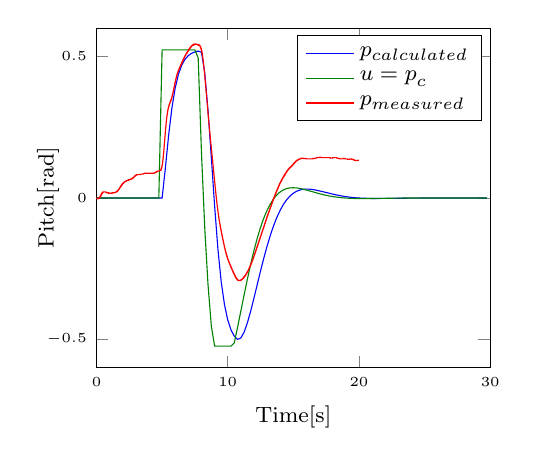
\begin{tikzpicture}

\begin{axis}[%
width = 5cm,
at={(0.758in,0.488in)},
scale only axis,
xmin=0,
xmax=30,
xlabel={\footnotesize{Time[s]}},
ymin=-0.6,
ymax=0.6,
ylabel={\footnotesize{Pitch[rad]}},
ylabel shift = -0.4cm,
axis background/.style={fill=white},
ticklabel style = {font=\tiny},
legend style={legend cell align=left, align=left, draw=black, font = \footnotesize}
]
\addplot [color=blue]
  table[row sep=crcr]{%
0	0\\
5	0\\
5.25	0.106028752058656\\
5.5	0.222660379323177\\
5.75	0.318881471816407\\
6	0.389443606311442\\
6.25	0.437955073776777\\
6.5	0.469972642303901\\
6.75	0.490517248775472\\
7	0.503431001414743\\
7.25	0.511421385860295\\
7.5	0.51630439857702\\
7.75	0.519258621270637\\
8	0.515203257617205\\
8.25	0.442077494057866\\
8.5	0.308917942206627\\
8.75	0.143857437412503\\
9	-0.026642171347433\\
9.25	-0.178852015358114\\
9.5	-0.294706712119982\\
9.75	-0.376103400744807\\
10	-0.430593712461647\\
10.25	-0.465910557041166\\
10.5	-0.488275766784287\\
10.75	-0.499764190883543\\
11	-0.494606006688155\\
11.25	-0.473847629784874\\
11.5	-0.440912018084063\\
11.75	-0.399653357456756\\
12	-0.353578675828111\\
12.5	-0.2579493548984\\
12.75	-0.212334914967485\\
13	-0.169924129646144\\
13.25	-0.131479200507158\\
13.5	-0.0974290818102865\\
13.75	-0.0679368059974763\\
14	-0.0429635308410177\\
14.25	-0.0223192342127767\\
14.5	-0.00570663885556044\\
14.75	0.00724201878417929\\
15	0.0169351049858726\\
15.25	0.0237983108610464\\
15.5	0.0282551996218636\\
15.75	0.03071226238756\\
16	0.0315508532381052\\
16.25	0.0311187961644848\\
16.5	0.029725886927416\\
16.75	0.0276432096833794\\
17.25	0.0222957734120826\\
18.25	0.0110954475341742\\
18.75	0.00659868322602009\\
19.25	0.003167897261946\\
19.75	0.000778241874598962\\
20.25	-0.000708334391688936\\
21	-0.00165871055146738\\
22	-0.00152183353077362\\
25	0\\
29.75	0\\
};
\addlegendentry{$\text{p}_{\text{calculated}}$}

\addplot [color=black!50!green]
  table[row sep=crcr]{%
0	0\\
4.75	0\\
5	0.523598775598298\\
7.5	0.523598775598298\\
7.75	0.494819035995317\\
8	0.160146388213864\\
8.25	-0.106263288038623\\
8.5	-0.307278306480395\\
8.75	-0.451544073993496\\
9	-0.523598775598298\\
10.25	-0.523598775598298\\
10.5	-0.511598967534702\\
10.75	-0.457129956387682\\
11.25	-0.342212060957365\\
11.5	-0.286365657156612\\
11.75	-0.233757373314109\\
12	-0.185424703030396\\
12.25	-0.142014857669654\\
12.5	-0.10385960931001\\
12.75	-0.0710390273514889\\
13	-0.0434270107361172\\
13.25	-0.0207605455327027\\
13.5	-0.0026532057262969\\
13.75	0.0113316469560196\\
14	0.0216778562869422\\
14.25	0.0288792627115377\\
14.5	0.0334210033379279\\
14.75	0.035766054664041\\
15	0.0363476842410009\\
15.25	0.0355551947305592\\
15.5	0.0337310214270481\\
15.75	0.0311830246785298\\
16.25	0.0248856506222559\\
17	0.0150402814094832\\
17.5	0.00942686961320049\\
18	0.00499923826903981\\
18.5	0.0017986264491725\\
19	-0.000289665822503338\\
19.5	-0.0014745362668549\\
20.25	-0.00203640858014609\\
21.25	-0.00156935527676438\\
23.5	-8.39090499056283e-05\\
26.25	0\\
29.75	0\\
};
\addlegendentry{$\text{u = p}_{\text{c}}$}

\addplot [color=red]
  table[row sep=crcr]{%
0	0\\
0.0100000000000016	0\\
0.0120000000000005	-0.00153398078788669\\
0.0579999999999998	-0.00153398078788669\\
0.0599999999999987	-0.00306796157576983\\
0.128	-0.00306796157576983\\
0.129999999999999	-0.00153398078788669\\
0.190000000000001	-0.00153398078788669\\
0.192	0\\
0.225999999999999	0\\
0.228000000000002	0.00153398078788669\\
0.245999999999999	0.00153398078788669\\
0.248000000000001	0.00306796157576983\\
0.266000000000002	0.00306796157576983\\
0.268000000000001	0.00460194236365652\\
0.294	0.00460194236365652\\
0.295999999999999	0.00613592315154321\\
0.308	0.00613592315154321\\
0.309999999999999	0.0076699039394299\\
0.324000000000002	0.0076699039394299\\
0.326000000000001	0.00920388472731304\\
0.34	0.00920388472731304\\
0.341999999999999	0.0107378655151997\\
0.356000000000002	0.0107378655151997\\
0.358000000000001	0.0122718463030864\\
0.361999999999998	0.0122718463030864\\
0.364000000000001	0.0107378655151997\\
0.366	0.0107378655151997\\
0.367999999999999	0.0122718463030864\\
0.382000000000001	0.0122718463030864\\
0.384	0.0138058270909696\\
0.396000000000001	0.0138058270909696\\
0.398	0.0153398078788562\\
0.411999999999999	0.0153398078788562\\
0.414000000000001	0.0168737886667429\\
0.416	0.0168737886667429\\
0.417999999999999	0.0153398078788562\\
0.423999999999999	0.0153398078788562\\
0.425999999999998	0.0168737886667429\\
0.437999999999999	0.0168737886667429\\
0.440000000000001	0.0184077694546261\\
0.446000000000002	0.0184077694546261\\
0.448	0.0168737886667429\\
0.449999999999999	0.0168737886667429\\
0.452000000000002	0.0184077694546261\\
0.466000000000001	0.0184077694546261\\
0.468	0.0199417502425128\\
0.474	0.0199417502425128\\
0.475999999999999	0.0184077694546261\\
0.478000000000002	0.0184077694546261\\
0.48	0.0199417502425128\\
0.481999999999999	0.0199417502425128\\
0.484000000000002	0.0214757310303995\\
0.486000000000001	0.0214757310303995\\
0.488	0.0199417502425128\\
0.494	0.0199417502425128\\
0.495999999999999	0.0214757310303995\\
0.5	0.0214757310303995\\
0.501999999999999	0.0199417502425128\\
0.507999999999999	0.0199417502425128\\
0.510000000000002	0.0214757310303995\\
0.518000000000001	0.0214757310303995\\
0.52	0.0199417502425128\\
0.521999999999998	0.0214757310303995\\
0.710000000000001	0.0214757310303995\\
0.712	0.0199417502425128\\
0.780000000000001	0.0199417502425128\\
0.782	0.0184077694546261\\
0.916	0.0184077694546261\\
0.917999999999999	0.0168737886667429\\
1.19	0.0168737886667429\\
1.192	0.0184077694546261\\
1.396	0.0184077694546261\\
1.398	0.0199417502425128\\
1.472	0.0199417502425128\\
1.474	0.0214757310303995\\
1.524	0.0214757310303995\\
1.526	0.0230097118182861\\
1.58	0.0230097118182861\\
1.582	0.0245436926061693\\
1.608	0.0245436926061693\\
1.61	0.026077673394056\\
1.642	0.026077673394056\\
1.644	0.0276116541819427\\
1.666	0.0276116541819427\\
1.668	0.0291456349698258\\
1.69	0.0291456349698258\\
1.692	0.0306796157577125\\
1.714	0.0306796157577125\\
1.716	0.0322135965455992\\
1.738	0.0322135965455992\\
1.74	0.0337475773334859\\
1.76	0.0337475773334859\\
1.762	0.035281558121369\\
1.782	0.035281558121369\\
1.784	0.0368155389092557\\
1.804	0.0368155389092557\\
1.806	0.0383495196971424\\
1.824	0.0383495196971424\\
1.826	0.0398835004850255\\
1.846	0.0398835004850255\\
1.848	0.0414174812729122\\
1.866	0.0414174812729122\\
1.868	0.0429514620607989\\
1.888	0.0429514620607989\\
1.89	0.0444854428486821\\
1.91	0.0444854428486821\\
1.912	0.0460194236365687\\
1.936	0.0460194236365687\\
1.938	0.0475534044244554\\
1.962	0.0475534044244554\\
1.964	0.0490873852123421\\
1.986	0.0490873852123421\\
1.988	0.0506213660002253\\
2.012	0.0506213660002253\\
2.014	0.052155346788112\\
2.048	0.052155346788112\\
2.05	0.0536893275759986\\
2.082	0.0536893275759986\\
2.084	0.0552233083638818\\
2.128	0.0552233083638818\\
2.13	0.0567572891517685\\
2.166	0.0567572891517685\\
2.168	0.0582912699396552\\
2.224	0.0582912699396552\\
2.226	0.0598252507275383\\
2.276	0.0598252507275383\\
2.278	0.061359231515425\\
2.354	0.061359231515425\\
2.356	0.0628932123033117\\
2.446	0.0628932123033117\\
2.448	0.0644271930911984\\
2.548	0.0644271930911984\\
2.55	0.0659611738790815\\
2.628	0.0659611738790815\\
2.63	0.0674951546669682\\
2.698	0.0674951546669682\\
2.7	0.0690291354548549\\
2.746	0.0690291354548549\\
2.748	0.070563116242738\\
2.79	0.070563116242738\\
2.792	0.0720970970306247\\
2.832	0.0720970970306247\\
2.834	0.0736310778185114\\
2.864	0.0736310778185114\\
2.866	0.0751650586063981\\
2.896	0.0751650586063981\\
2.898	0.0766990393942812\\
2.93	0.0766990393942812\\
2.932	0.0782330201821679\\
2.97	0.0782330201821679\\
2.972	0.0797670009700546\\
3.012	0.0797670009700546\\
3.014	0.0813009817579378\\
3.056	0.0813009817579378\\
3.058	0.0828349625458245\\
3.356	0.0828349625458245\\
3.358	0.0843689433337111\\
3.554	0.0843689433337111\\
3.556	0.0859029241215943\\
3.668	0.0859029241215943\\
3.67	0.087436904909481\\
4.386	0.087436904909481\\
4.388	0.0889708856973677\\
4.472	0.0889708856973677\\
4.474	0.0905048664852544\\
4.53	0.0905048664852544\\
4.532	0.0920388472731375\\
4.588	0.0920388472731375\\
4.59	0.0935728280610242\\
4.652	0.0935728280610242\\
4.654	0.0951068088489109\\
4.77	0.0951068088489109\\
4.772	0.096640789636794\\
4.874	0.096640789636794\\
4.876	0.0981747704246807\\
4.902	0.0981747704246807\\
4.904	0.0997087512125674\\
4.916	0.0997087512125674\\
4.918	0.101242732000454\\
4.93	0.101242732000454\\
4.932	0.102776712788337\\
4.944	0.102776712788337\\
4.946	0.104310693576224\\
4.954	0.104310693576224\\
4.956	0.105844674364111\\
4.964	0.105844674364111\\
4.966	0.107378655151994\\
4.974	0.107378655151994\\
4.976	0.10891263593988\\
4.978	0.10891263593988\\
4.98	0.110446616727767\\
4.988	0.110446616727767\\
4.992	0.113514578303537\\
5	0.113514578303537\\
5.002	0.115048559091424\\
5.004	0.115048559091424\\
5.006	0.11658253987931\\
5.012	0.11658253987931\\
5.016	0.11965050145508\\
5.022	0.11965050145508\\
5.024	0.121184482242967\\
5.026	0.121184482242967\\
5.028	0.12271846303085\\
5.03	0.12271846303085\\
5.032	0.124252443818737\\
5.036	0.124252443818737\\
5.038	0.125786424606623\\
5.04	0.125786424606623\\
5.042	0.127320405394507\\
5.044	0.127320405394507\\
5.046	0.128854386182393\\
5.048	0.128854386182393\\
5.05	0.13038836697028\\
5.052	0.13038836697028\\
5.054	0.131922347758167\\
5.056	0.131922347758167\\
5.058	0.13345632854605\\
5.06	0.13345632854605\\
5.062	0.134990309333936\\
5.064	0.134990309333936\\
5.066	0.136524290121823\\
5.068	0.136524290121823\\
5.07	0.138058270909706\\
5.072	0.138058270909706\\
5.076	0.14112623248548\\
5.078	0.14112623248548\\
5.08	0.142660213273366\\
5.082	0.142660213273366\\
5.084	0.144194194061249\\
5.086	0.144194194061249\\
5.09	0.147262155637023\\
5.092	0.147262155637023\\
5.094	0.148796136424906\\
5.096	0.148796136424906\\
5.1	0.151864098000679\\
5.102	0.151864098000679\\
5.106	0.154932059576449\\
5.108	0.154932059576449\\
5.112	0.158000021152223\\
5.114	0.158000021152223\\
5.116	0.159534001940106\\
5.118	0.159534001940106\\
5.122	0.162601963515879\\
5.124	0.162601963515879\\
5.13	0.167203905879536\\
5.132	0.167203905879536\\
5.138	0.171805848243192\\
5.14	0.171805848243192\\
5.142	0.173339829031079\\
5.144	0.173339829031079\\
5.152	0.179475752182618\\
5.154	0.179475752182618\\
5.156	0.181009732970505\\
5.158	0.181009732970505\\
5.166	0.187145656122048\\
5.168	0.187145656122048\\
5.17	0.188679636909935\\
5.172	0.188679636909935\\
5.18	0.194815560061475\\
5.182	0.194815560061475\\
5.19	0.200951483213018\\
5.194	0.200951483213018\\
5.204	0.208621387152448\\
5.206	0.208621387152448\\
5.212	0.213223329516104\\
5.214	0.213223329516104\\
5.218	0.216291291091874\\
5.22	0.216291291091874\\
5.228	0.222427214243417\\
5.23	0.222427214243417\\
5.232	0.223961195031304\\
5.234	0.223961195031304\\
5.242	0.230097118182847\\
5.244	0.230097118182847\\
5.248	0.233165079758617\\
5.25	0.233165079758617\\
5.254	0.23623304133439\\
5.256	0.23623304133439\\
5.264	0.24236896448593\\
5.266	0.24236896448593\\
5.268	0.243902945273817\\
5.27	0.243902945273817\\
5.278	0.25003886842536\\
5.282	0.25003886842536\\
5.29	0.256174791576903\\
5.296	0.256174791576903\\
5.298	0.257708772364786\\
5.3	0.26077673394056\\
5.302	0.262310714728443\\
5.308	0.262310714728443\\
5.316	0.268446637879986\\
5.32	0.268446637879986\\
5.326	0.273048580243643\\
5.332	0.273048580243643\\
5.34	0.279184503395186\\
5.346	0.279184503395186\\
5.352	0.283786445758842\\
5.358	0.283786445758842\\
5.364	0.288388388122499\\
5.37	0.288388388122499\\
5.376	0.292990330486159\\
5.378	0.292990330486159\\
5.38	0.291456349698272\\
5.388	0.297592272849815\\
5.39	0.296058292061929\\
5.394	0.296058292061929\\
5.4	0.300660234425585\\
5.402	0.300660234425585\\
5.404	0.299126253637699\\
5.406	0.299126253637699\\
5.408	0.300660234425585\\
5.41	0.303728196001359\\
5.412	0.303728196001359\\
5.414	0.305262176789242\\
5.416	0.303728196001359\\
5.418	0.303728196001359\\
5.424	0.308330138365015\\
5.426	0.308330138365015\\
5.428	0.306796157577129\\
5.43	0.306796157577129\\
5.436	0.311398099940785\\
5.438	0.311398099940785\\
5.44	0.309864119152898\\
5.442	0.309864119152898\\
5.446	0.312932080728672\\
5.448	0.312932080728672\\
5.45	0.314466061516555\\
5.452	0.312932080728672\\
5.456	0.312932080728672\\
5.46	0.316000042304442\\
5.468	0.316000042304442\\
5.472	0.319068003880215\\
5.476	0.319068003880215\\
5.478	0.317534023092328\\
5.48	0.317534023092328\\
5.486	0.322135965455985\\
5.488	0.320601984668098\\
5.494	0.320601984668098\\
5.498	0.323669946243871\\
5.5	0.323669946243871\\
5.502	0.322135965455985\\
5.504	0.322135965455985\\
5.506	0.323669946243871\\
5.508	0.323669946243871\\
5.51	0.325203927031755\\
5.514	0.325203927031755\\
5.516	0.323669946243871\\
5.518	0.325203927031755\\
5.52	0.325203927031755\\
5.522	0.326737907819641\\
5.53	0.326737907819641\\
5.532	0.328271888607528\\
5.542	0.328271888607528\\
5.544	0.329805869395411\\
5.554	0.329805869395411\\
5.556	0.331339850183298\\
5.566	0.331339850183298\\
5.568	0.332873830971185\\
5.578	0.332873830971185\\
5.58	0.334407811759071\\
5.59	0.334407811759071\\
5.592	0.335941792546954\\
5.602	0.335941792546954\\
5.604	0.337475773334841\\
5.616	0.337475773334841\\
5.618	0.339009754122728\\
5.628	0.339009754122728\\
5.63	0.340543734910611\\
5.642	0.340543734910611\\
5.644	0.342077715698498\\
5.654	0.342077715698498\\
5.656	0.343611696486384\\
5.666	0.343611696486384\\
5.668	0.345145677274271\\
5.676	0.345145677274271\\
5.678	0.346679658062154\\
5.688	0.346679658062154\\
5.69	0.348213638850041\\
5.7	0.348213638850041\\
5.702	0.349747619637927\\
5.712	0.349747619637927\\
5.714	0.351281600425811\\
5.722	0.351281600425811\\
5.724	0.352815581213697\\
5.73	0.352815581213697\\
5.732	0.354349562001584\\
5.738	0.354349562001584\\
5.74	0.355883542789467\\
5.748	0.355883542789467\\
5.75	0.357417523577354\\
5.758	0.357417523577354\\
5.76	0.35895150436524\\
5.766	0.35895150436524\\
5.768	0.360485485153127\\
5.774	0.360485485153127\\
5.776	0.36201946594101\\
5.784	0.36201946594101\\
5.786	0.363553446728897\\
5.79	0.363553446728897\\
5.792	0.365087427516784\\
5.798	0.365087427516784\\
5.8	0.366621408304667\\
5.806	0.366621408304667\\
5.808	0.368155389092554\\
5.816	0.368155389092554\\
5.818	0.36968936988044\\
5.82	0.36968936988044\\
5.822	0.371223350668327\\
5.83	0.371223350668327\\
5.832	0.37275733145621\\
5.834	0.37275733145621\\
5.836	0.374291312244097\\
5.844	0.374291312244097\\
5.846	0.375825293031983\\
5.85	0.375825293031983\\
5.852	0.377359273819867\\
5.858	0.377359273819867\\
5.86	0.378893254607753\\
5.864	0.378893254607753\\
5.866	0.38042723539564\\
5.872	0.38042723539564\\
5.874	0.381961216183523\\
5.878	0.381961216183523\\
5.88	0.38349519697141\\
5.886	0.38349519697141\\
5.888	0.385029177759296\\
5.892	0.385029177759296\\
5.894	0.386563158547183\\
5.9	0.386563158547183\\
5.902	0.388097139335066\\
5.906	0.388097139335066\\
5.908	0.389631120122953\\
5.914	0.389631120122953\\
5.916	0.39116510091084\\
5.918	0.39116510091084\\
5.92	0.392699081698723\\
5.928	0.392699081698723\\
5.93	0.394233062486609\\
5.932	0.394233062486609\\
5.934	0.395767043274496\\
5.94	0.395767043274496\\
5.942	0.397301024062379\\
5.948	0.397301024062379\\
5.95	0.398835004850266\\
5.954	0.398835004850266\\
5.956	0.400368985638153\\
5.96	0.400368985638153\\
5.962	0.401902966426039\\
5.968	0.401902966426039\\
5.97	0.403436947213923\\
5.974	0.403436947213923\\
5.976	0.404970928001809\\
5.982	0.404970928001809\\
5.984	0.406504908789696\\
5.988	0.406504908789696\\
5.99	0.408038889577579\\
5.996	0.408038889577579\\
5.998	0.409572870365466\\
6.002	0.409572870365466\\
6.004	0.411106851153352\\
6.01	0.411106851153352\\
6.012	0.412640831941239\\
6.016	0.412640831941239\\
6.018	0.414174812729122\\
6.024	0.414174812729122\\
6.026	0.415708793517009\\
6.032	0.415708793517009\\
6.034	0.417242774304896\\
6.04	0.417242774304896\\
6.042	0.418776755092779\\
6.046	0.418776755092779\\
6.048	0.420310735880665\\
6.054	0.420310735880665\\
6.056	0.421844716668552\\
6.062	0.421844716668552\\
6.064	0.423378697456435\\
6.07	0.423378697456435\\
6.072	0.424912678244322\\
6.078	0.424912678244322\\
6.08	0.426446659032209\\
6.086	0.426446659032209\\
6.088	0.427980639820095\\
6.096	0.427980639820095\\
6.098	0.429514620607979\\
6.104	0.429514620607979\\
6.106	0.431048601395865\\
6.114	0.431048601395865\\
6.116	0.432582582183752\\
6.122	0.432582582183752\\
6.124	0.434116562971635\\
6.132	0.434116562971635\\
6.134	0.435650543759522\\
6.142	0.435650543759522\\
6.144	0.437184524547408\\
6.152	0.437184524547408\\
6.154	0.438718505335295\\
6.162	0.438718505335295\\
6.164	0.440252486123178\\
6.172	0.440252486123178\\
6.174	0.441786466911065\\
6.184	0.441786466911065\\
6.186	0.443320447698952\\
6.194	0.443320447698952\\
6.196	0.444854428486835\\
6.206	0.444854428486835\\
6.208	0.446388409274721\\
6.218	0.446388409274721\\
6.22	0.447922390062608\\
6.23	0.447922390062608\\
6.232	0.449456370850491\\
6.244	0.449456370850491\\
6.246	0.450990351638378\\
6.258	0.450990351638378\\
6.26	0.452524332426265\\
6.27	0.452524332426265\\
6.272	0.454058313214151\\
6.284	0.454058313214151\\
6.286	0.455592294002034\\
6.298	0.455592294002034\\
6.3	0.457126274789921\\
6.312	0.457126274789921\\
6.314	0.458660255577808\\
6.324	0.458660255577808\\
6.326	0.460194236365691\\
6.34	0.460194236365691\\
6.342	0.461728217153578\\
6.354	0.461728217153578\\
6.356	0.463262197941464\\
6.374	0.463262197941464\\
6.376	0.464796178729351\\
6.386	0.464796178729351\\
6.388	0.466330159517234\\
6.4	0.466330159517234\\
6.402	0.467864140305121\\
6.414	0.467864140305121\\
6.416	0.469398121093008\\
6.428	0.469398121093008\\
6.43	0.470932101880891\\
6.442	0.470932101880891\\
6.444	0.472466082668777\\
6.464	0.472466082668777\\
6.466	0.474000063456664\\
6.476	0.474000063456664\\
6.478	0.475534044244547\\
6.49	0.475534044244547\\
6.492	0.477068025032434\\
6.502	0.477068025032434\\
6.504	0.478602005820321\\
6.516	0.478602005820321\\
6.518	0.480135986608207\\
6.53	0.480135986608207\\
6.532	0.48166996739609\\
6.536	0.48166996739609\\
6.538	0.480135986608207\\
6.54	0.48166996739609\\
6.552	0.48166996739609\\
6.554	0.483203948183977\\
6.566	0.483203948183977\\
6.568	0.484737928971864\\
6.578	0.484737928971864\\
6.58	0.486271909759747\\
6.592	0.486271909759747\\
6.594	0.487805890547634\\
6.614	0.487805890547634\\
6.616	0.48933987133552\\
6.626	0.48933987133552\\
6.628	0.490873852123404\\
6.64	0.490873852123404\\
6.642	0.49240783291129\\
6.654	0.49240783291129\\
6.656	0.493941813699177\\
6.672	0.493941813699177\\
6.674	0.495475794487064\\
6.688	0.495475794487064\\
6.69	0.497009775274947\\
6.704	0.497009775274947\\
6.706	0.498543756062833\\
6.722	0.498543756062833\\
6.724	0.50007773685072\\
6.738	0.50007773685072\\
6.74	0.501611717638603\\
6.76	0.501611717638603\\
6.762	0.50314569842649\\
6.774	0.50314569842649\\
6.776	0.504679679214377\\
6.79	0.504679679214377\\
6.792	0.506213660002263\\
6.794	0.506213660002263\\
6.796	0.504679679214377\\
6.798	0.504679679214377\\
6.8	0.506213660002263\\
6.812	0.506213660002263\\
6.814	0.507747640790146\\
6.826	0.507747640790146\\
6.828	0.509281621578033\\
6.83	0.509281621578033\\
6.832	0.507747640790146\\
6.836	0.507747640790146\\
6.838	0.509281621578033\\
6.85	0.509281621578033\\
6.852	0.51081560236592\\
6.858	0.51081560236592\\
6.86	0.509281621578033\\
6.862	0.51081560236592\\
6.864	0.51081560236592\\
6.866	0.512349583153803\\
6.868	0.512349583153803\\
6.87	0.51081560236592\\
6.874	0.51081560236592\\
6.876	0.512349583153803\\
6.888	0.512349583153803\\
6.89	0.51388356394169\\
6.894	0.51388356394169\\
6.896	0.512349583153803\\
6.898	0.512349583153803\\
6.9	0.51388356394169\\
6.912	0.51388356394169\\
6.914	0.515417544729576\\
6.926	0.515417544729576\\
6.928	0.516951525517459\\
6.93	0.516951525517459\\
6.932	0.515417544729576\\
6.936	0.515417544729576\\
6.938	0.516951525517459\\
6.95	0.516951525517459\\
6.952	0.518485506305346\\
6.958	0.518485506305346\\
6.96	0.516951525517459\\
6.962	0.518485506305346\\
6.966	0.518485506305346\\
6.968	0.520019487093233\\
6.97	0.518485506305346\\
6.974	0.518485506305346\\
6.976	0.520019487093233\\
6.988	0.520019487093233\\
6.99	0.52155346788112\\
6.994	0.52155346788112\\
6.996	0.520019487093233\\
6.998	0.520019487093233\\
7	0.52155346788112\\
7.012	0.52155346788112\\
7.014	0.523087448669003\\
7.026	0.523087448669003\\
7.028	0.524621429456889\\
7.03	0.524621429456889\\
7.032	0.523087448669003\\
7.036	0.523087448669003\\
7.038	0.524621429456889\\
7.052	0.524621429456889\\
7.054	0.526155410244776\\
7.056	0.526155410244776\\
7.058	0.524621429456889\\
7.06	0.524621429456889\\
7.062	0.526155410244776\\
7.074	0.526155410244776\\
7.076	0.527689391032659\\
7.1	0.527689391032659\\
7.102	0.529223371820546\\
7.116	0.529223371820546\\
7.118	0.530757352608433\\
7.12	0.529223371820546\\
7.124	0.529223371820546\\
7.126	0.530757352608433\\
7.148	0.530757352608433\\
7.15	0.532291333396319\\
7.174	0.532291333396319\\
7.176	0.533825314184202\\
7.2	0.533825314184202\\
7.202	0.535359294972089\\
7.23	0.535359294972089\\
7.232	0.536893275759976\\
7.268	0.536893275759976\\
7.27	0.538427256547859\\
7.294	0.538427256547859\\
7.296	0.539961237335746\\
7.298	0.539961237335746\\
7.3	0.538427256547859\\
7.304	0.538427256547859\\
7.306	0.539961237335746\\
7.332	0.539961237335746\\
7.334	0.541495218123632\\
7.336	0.539961237335746\\
7.342	0.539961237335746\\
7.344	0.541495218123632\\
7.348	0.541495218123632\\
7.35	0.539961237335746\\
7.354	0.539961237335746\\
7.356	0.541495218123632\\
7.362	0.541495218123632\\
7.364	0.539961237335746\\
7.366	0.541495218123632\\
7.38	0.541495218123632\\
7.382	0.543029198911515\\
7.384	0.543029198911515\\
7.386	0.541495218123632\\
7.392	0.541495218123632\\
7.394	0.543029198911515\\
7.398	0.543029198911515\\
7.4	0.541495218123632\\
7.404	0.541495218123632\\
7.406	0.543029198911515\\
7.41	0.543029198911515\\
7.412	0.541495218123632\\
7.416	0.541495218123632\\
7.418	0.543029198911515\\
7.422	0.543029198911515\\
7.424	0.541495218123632\\
7.428	0.541495218123632\\
7.43	0.543029198911515\\
7.436	0.543029198911515\\
7.438	0.541495218123632\\
7.44	0.541495218123632\\
7.444	0.544563179699402\\
7.446	0.544563179699402\\
7.45	0.541495218123632\\
7.452	0.541495218123632\\
7.456	0.544563179699402\\
7.458	0.544563179699402\\
7.462	0.541495218123632\\
7.464	0.541495218123632\\
7.468	0.544563179699402\\
7.47	0.544563179699402\\
7.474	0.541495218123632\\
7.476	0.541495218123632\\
7.48	0.544563179699402\\
7.482	0.544563179699402\\
7.484	0.543029198911515\\
7.486	0.543029198911515\\
7.488	0.541495218123632\\
7.492	0.544563179699402\\
7.496	0.544563179699402\\
7.498	0.543029198911515\\
7.502	0.543029198911515\\
7.504	0.544563179699402\\
7.508	0.544563179699402\\
7.51	0.543029198911515\\
7.514	0.543029198911515\\
7.516	0.544563179699402\\
7.52	0.544563179699402\\
7.522	0.543029198911515\\
7.526	0.543029198911515\\
7.528	0.544563179699402\\
7.532	0.544563179699402\\
7.534	0.543029198911515\\
7.538	0.543029198911515\\
7.54	0.544563179699402\\
7.544	0.544563179699402\\
7.546	0.543029198911515\\
7.552	0.543029198911515\\
7.554	0.544563179699402\\
7.556	0.544563179699402\\
7.558	0.543029198911515\\
7.564	0.543029198911515\\
7.566	0.544563179699402\\
7.568	0.544563179699402\\
7.57	0.543029198911515\\
7.576	0.543029198911515\\
7.578	0.544563179699402\\
7.58	0.544563179699402\\
7.582	0.543029198911515\\
7.588	0.543029198911515\\
7.59	0.544563179699402\\
7.592	0.543029198911515\\
7.646	0.543029198911515\\
7.648	0.544563179699402\\
7.65	0.543029198911515\\
7.658	0.543029198911515\\
7.66	0.544563179699402\\
7.662	0.543029198911515\\
7.67	0.543029198911515\\
7.672	0.544563179699402\\
7.674	0.543029198911515\\
7.676	0.543029198911515\\
7.678	0.541495218123632\\
7.68	0.543029198911515\\
7.682	0.543029198911515\\
7.684	0.544563179699402\\
7.688	0.541495218123632\\
7.69	0.541495218123632\\
7.692	0.543029198911515\\
7.694	0.543029198911515\\
7.696	0.544563179699402\\
7.7	0.541495218123632\\
7.702	0.541495218123632\\
7.704	0.543029198911515\\
7.706	0.543029198911515\\
7.708	0.544563179699402\\
7.712	0.541495218123632\\
7.716	0.541495218123632\\
7.718	0.543029198911515\\
7.722	0.543029198911515\\
7.724	0.541495218123632\\
7.728	0.541495218123632\\
7.73	0.543029198911515\\
7.734	0.543029198911515\\
7.736	0.541495218123632\\
7.74	0.541495218123632\\
7.742	0.543029198911515\\
7.746	0.543029198911515\\
7.748	0.541495218123632\\
7.754	0.541495218123632\\
7.756	0.543029198911515\\
7.758	0.543029198911515\\
7.762	0.539961237335746\\
7.764	0.541495218123632\\
7.766	0.541495218123632\\
7.768	0.543029198911515\\
7.77	0.543029198911515\\
7.774	0.539961237335746\\
7.776	0.539961237335746\\
7.778	0.541495218123632\\
7.784	0.541495218123632\\
7.786	0.539961237335746\\
7.788	0.539961237335746\\
7.79	0.541495218123632\\
7.796	0.541495218123632\\
7.798	0.539961237335746\\
7.802	0.539961237335746\\
7.804	0.541495218123632\\
7.806	0.541495218123632\\
7.808	0.539961237335746\\
7.84	0.539961237335746\\
7.842	0.538427256547859\\
7.844	0.538427256547859\\
7.846	0.539961237335746\\
7.848	0.539961237335746\\
7.85	0.538427256547859\\
7.864	0.538427256547859\\
7.866	0.536893275759976\\
7.868	0.538427256547859\\
7.874	0.538427256547859\\
7.876	0.536893275759976\\
7.882	0.536893275759976\\
7.884	0.538427256547859\\
7.886	0.536893275759976\\
7.888	0.536893275759976\\
7.89	0.535359294972089\\
7.892	0.536893275759976\\
7.898	0.536893275759976\\
7.9	0.535359294972089\\
7.906	0.535359294972089\\
7.908	0.536893275759976\\
7.912	0.533825314184202\\
7.916	0.533825314184202\\
7.918	0.535359294972089\\
7.922	0.535359294972089\\
7.926	0.532291333396319\\
7.928	0.532291333396319\\
7.93	0.533825314184202\\
7.934	0.533825314184202\\
7.938	0.530757352608433\\
7.94	0.530757352608433\\
7.944	0.533825314184202\\
7.95	0.529223371820546\\
7.952	0.529223371820546\\
7.956	0.532291333396319\\
7.962	0.527689391032659\\
7.964	0.527689391032659\\
7.968	0.530757352608433\\
7.974	0.526155410244776\\
7.976	0.526155410244776\\
7.978	0.527689391032659\\
7.982	0.527689391032659\\
7.986	0.524621429456889\\
7.99	0.524621429456889\\
7.992	0.526155410244776\\
7.994	0.526155410244776\\
7.996	0.524621429456889\\
7.998	0.52155346788112\\
8	0.52155346788112\\
8.004	0.524621429456889\\
8.01	0.520019487093233\\
8.014	0.520019487093233\\
8.016	0.52155346788112\\
8.018	0.52155346788112\\
8.02	0.520019487093233\\
8.022	0.516951525517459\\
8.026	0.516951525517459\\
8.028	0.518485506305346\\
8.03	0.518485506305346\\
8.032	0.516951525517459\\
8.034	0.51388356394169\\
8.036	0.51388356394169\\
8.038	0.515417544729576\\
8.042	0.515417544729576\\
8.048	0.51081560236592\\
8.05	0.512349583153803\\
8.054	0.512349583153803\\
8.06	0.507747640790146\\
8.062	0.507747640790146\\
8.064	0.509281621578033\\
8.066	0.509281621578033\\
8.068	0.507747640790146\\
8.07	0.504679679214377\\
8.074	0.504679679214377\\
8.076	0.506213660002263\\
8.082	0.501611717638603\\
8.09	0.501611717638603\\
8.096	0.497009775274947\\
8.102	0.497009775274947\\
8.106	0.493941813699177\\
8.112	0.493941813699177\\
8.118	0.48933987133552\\
8.124	0.48933987133552\\
8.128	0.486271909759747\\
8.13	0.486271909759747\\
8.132	0.484737928971864\\
8.136	0.484737928971864\\
8.14	0.48166996739609\\
8.146	0.48166996739609\\
8.154	0.475534044244547\\
8.16	0.475534044244547\\
8.166	0.470932101880891\\
8.17	0.470932101880891\\
8.176	0.466330159517234\\
8.182	0.466330159517234\\
8.188	0.461728217153578\\
8.194	0.461728217153578\\
8.196	0.460194236365691\\
8.198	0.457126274789921\\
8.2	0.455592294002034\\
8.206	0.455592294002034\\
8.214	0.449456370850491\\
8.216	0.449456370850491\\
8.218	0.450990351638378\\
8.22	0.449456370850491\\
8.222	0.446388409274721\\
8.224	0.444854428486835\\
8.23	0.444854428486835\\
8.232	0.443320447698952\\
8.234	0.440252486123178\\
8.236	0.438718505335295\\
8.242	0.438718505335295\\
8.244	0.437184524547408\\
8.246	0.434116562971635\\
8.248	0.432582582183752\\
8.254	0.432582582183752\\
8.258	0.429514620607979\\
8.26	0.426446659032209\\
8.266	0.426446659032209\\
8.27	0.423378697456435\\
8.272	0.420310735880665\\
8.28	0.420310735880665\\
8.284	0.414174812729122\\
8.292	0.414174812729122\\
8.294	0.411106851153352\\
8.298	0.408038889577579\\
8.304	0.408038889577579\\
8.308	0.401902966426039\\
8.316	0.401902966426039\\
8.32	0.395767043274496\\
8.326	0.395767043274496\\
8.33	0.392699081698723\\
8.332	0.389631120122953\\
8.338	0.389631120122953\\
8.342	0.386563158547183\\
8.344	0.38349519697141\\
8.346	0.381961216183523\\
8.352	0.381961216183523\\
8.354	0.38042723539564\\
8.356	0.377359273819867\\
8.358	0.375825293031983\\
8.364	0.375825293031983\\
8.366	0.374291312244097\\
8.368	0.371223350668327\\
8.37	0.36968936988044\\
8.374	0.36968936988044\\
8.382	0.363553446728897\\
8.384	0.363553446728897\\
8.386	0.36201946594101\\
8.388	0.36201946594101\\
8.396	0.355883542789467\\
8.398	0.355883542789467\\
8.4	0.354349562001584\\
8.402	0.354349562001584\\
8.408	0.349747619637927\\
8.41	0.349747619637927\\
8.414	0.346679658062154\\
8.416	0.346679658062154\\
8.422	0.342077715698498\\
8.424	0.342077715698498\\
8.428	0.339009754122728\\
8.43	0.339009754122728\\
8.436	0.334407811759071\\
8.438	0.334407811759071\\
8.442	0.331339850183298\\
8.444	0.331339850183298\\
8.45	0.326737907819641\\
8.452	0.326737907819641\\
8.454	0.325203927031755\\
8.456	0.325203927031755\\
8.464	0.319068003880215\\
8.466	0.319068003880215\\
8.472	0.314466061516555\\
8.474	0.314466061516555\\
8.476	0.312932080728672\\
8.478	0.312932080728672\\
8.486	0.306796157577129\\
8.49	0.306796157577129\\
8.498	0.300660234425585\\
8.5	0.300660234425585\\
8.502	0.299126253637699\\
8.504	0.299126253637699\\
8.51	0.294524311274042\\
8.512	0.294524311274042\\
8.514	0.292990330486159\\
8.516	0.292990330486159\\
8.524	0.286854407334616\\
8.526	0.286854407334616\\
8.528	0.285320426546729\\
8.53	0.285320426546729\\
8.536	0.280718484183073\\
8.538	0.280718484183073\\
8.54	0.279184503395186\\
8.542	0.279184503395186\\
8.548	0.274582561031529\\
8.55	0.274582561031529\\
8.554	0.27151459945576\\
8.556	0.27151459945576\\
8.56	0.268446637879986\\
8.562	0.268446637879986\\
8.568	0.26384469551633\\
8.572	0.26384469551633\\
8.58	0.257708772364786\\
8.584	0.257708772364786\\
8.586	0.256174791576903\\
8.588	0.256174791576903\\
8.59	0.254640810789017\\
8.592	0.251572849213247\\
8.596	0.251572849213247\\
8.598	0.25003886842536\\
8.6	0.25003886842536\\
8.602	0.248504887637473\\
8.604	0.245436926061704\\
8.608	0.245436926061704\\
8.61	0.243902945273817\\
8.612	0.243902945273817\\
8.618	0.23930100291016\\
8.62	0.23930100291016\\
8.622	0.237767022122274\\
8.624	0.237767022122274\\
8.63	0.233165079758617\\
8.634	0.233165079758617\\
8.642	0.227029156607074\\
8.646	0.227029156607074\\
8.648	0.225495175819191\\
8.65	0.225495175819191\\
8.656	0.220893233455531\\
8.66	0.220893233455531\\
8.668	0.214757310303991\\
8.672	0.214757310303991\\
8.678	0.210155367940335\\
8.68	0.210155367940335\\
8.682	0.208621387152448\\
8.684	0.208621387152448\\
8.688	0.205553425576674\\
8.69	0.205553425576674\\
8.692	0.204019444788791\\
8.694	0.204019444788791\\
8.696	0.202485464000905\\
8.698	0.202485464000905\\
8.704	0.197883521637248\\
8.708	0.197883521637248\\
8.714	0.193281579273592\\
8.716	0.193281579273592\\
8.718	0.191747598485705\\
8.72	0.191747598485705\\
8.726	0.187145656122048\\
8.732	0.187145656122048\\
8.74	0.181009732970505\\
8.744	0.181009732970505\\
8.75	0.176407790606849\\
8.754	0.176407790606849\\
8.756	0.174873809818962\\
8.758	0.174873809818962\\
8.76	0.173339829031079\\
8.762	0.170271867455305\\
8.768	0.170271867455305\\
8.776	0.164135944303762\\
8.782	0.164135944303762\\
8.784	0.161067982727992\\
8.786	0.159534001940106\\
8.792	0.159534001940106\\
8.8	0.153398078788562\\
8.806	0.153398078788562\\
8.808	0.150330117212793\\
8.812	0.147262155637023\\
8.818	0.147262155637023\\
8.826	0.14112623248548\\
8.832	0.14112623248548\\
8.834	0.138058270909706\\
8.836	0.136524290121823\\
8.842	0.136524290121823\\
8.846	0.13345632854605\\
8.848	0.13038836697028\\
8.856	0.13038836697028\\
8.858	0.127320405394507\\
8.862	0.124252443818737\\
8.868	0.124252443818737\\
8.87	0.12271846303085\\
8.872	0.11965050145508\\
8.874	0.118116520667193\\
8.88	0.118116520667193\\
8.886	0.113514578303537\\
8.892	0.113514578303537\\
8.894	0.11198059751565\\
8.896	0.10891263593988\\
8.898	0.107378655151994\\
8.904	0.107378655151994\\
8.912	0.101242732000454\\
8.918	0.101242732000454\\
8.92	0.0981747704246807\\
8.924	0.0951068088489109\\
8.93	0.0951068088489109\\
8.932	0.0935728280610242\\
8.934	0.0905048664852544\\
8.936	0.0889708856973677\\
8.942	0.0889708856973677\\
8.948	0.0843689433337111\\
8.954	0.0843689433337111\\
8.956	0.0828349625458245\\
8.958	0.0797670009700546\\
8.96	0.0782330201821679\\
8.966	0.0782330201821679\\
8.974	0.0720970970306247\\
8.98	0.0720970970306247\\
8.982	0.0690291354548549\\
8.986	0.0659611738790815\\
8.992	0.0659611738790815\\
8.994	0.0644271930911984\\
8.996	0.061359231515425\\
8.998	0.061359231515425\\
9	0.0598252507275383\\
9.004	0.0598252507275383\\
9.01	0.0552233083638818\\
9.014	0.0552233083638818\\
9.016	0.0536893275759986\\
9.018	0.0536893275759986\\
9.02	0.0506213660002253\\
9.022	0.0490873852123421\\
9.028	0.0490873852123421\\
9.036	0.0429514620607989\\
9.04	0.0429514620607989\\
9.046	0.0383495196971424\\
9.05	0.0383495196971424\\
9.052	0.0368155389092557\\
9.054	0.0368155389092557\\
9.06	0.0322135965455992\\
9.064	0.0322135965455992\\
9.07	0.0276116541819427\\
9.072	0.0276116541819427\\
9.074	0.026077673394056\\
9.078	0.026077673394056\\
9.084	0.0214757310303995\\
9.088	0.0214757310303995\\
9.094	0.0168737886667429\\
9.096	0.0168737886667429\\
9.098	0.0153398078788562\\
9.102	0.0153398078788562\\
9.108	0.0107378655151997\\
9.112	0.0107378655151997\\
9.116	0.0076699039394299\\
9.118	0.0076699039394299\\
9.12	0.00613592315154321\\
9.122	0.00613592315154321\\
9.124	0.00460194236365652\\
9.126	0.00460194236365652\\
9.13	0.00153398078788669\\
9.132	0.00153398078788669\\
9.134	0\\
9.136	0\\
9.138	-0.00153398078788669\\
9.14	-0.00153398078788669\\
9.144	-0.00460194236365652\\
9.148	-0.00460194236365652\\
9.154	-0.00920388472731304\\
9.16	-0.00920388472731304\\
9.166	-0.0138058270909696\\
9.168	-0.0138058270909696\\
9.17	-0.0153398078788562\\
9.174	-0.0153398078788562\\
9.18	-0.0199417502425128\\
9.186	-0.0199417502425128\\
9.192	-0.0245436926061693\\
9.198	-0.0245436926061693\\
9.204	-0.0291456349698258\\
9.21	-0.0291456349698258\\
9.216	-0.0337475773334859\\
9.222	-0.0337475773334859\\
9.228	-0.0383495196971424\\
9.236	-0.0383495196971424\\
9.242	-0.0429514620607989\\
9.248	-0.0429514620607989\\
9.254	-0.0475534044244554\\
9.26	-0.0475534044244554\\
9.264	-0.0506213660002253\\
9.266	-0.0506213660002253\\
9.268	-0.052155346788112\\
9.274	-0.052155346788112\\
9.278	-0.0552233083638818\\
9.284	-0.0552233083638818\\
9.288	-0.0582912699396552\\
9.29	-0.0582912699396552\\
9.292	-0.0598252507275383\\
9.296	-0.0598252507275383\\
9.298	-0.061359231515425\\
9.3	-0.061359231515425\\
9.302	-0.0628932123033117\\
9.306	-0.0628932123033117\\
9.308	-0.0644271930911984\\
9.31	-0.0644271930911984\\
9.312	-0.0659611738790815\\
9.314	-0.0659611738790815\\
9.316	-0.0674951546669682\\
9.322	-0.0674951546669682\\
9.326	-0.070563116242738\\
9.332	-0.070563116242738\\
9.336	-0.0736310778185114\\
9.338	-0.0736310778185114\\
9.34	-0.0751650586063981\\
9.346	-0.0751650586063981\\
9.348	-0.0766990393942812\\
9.35	-0.0766990393942812\\
9.352	-0.0782330201821679\\
9.358	-0.0782330201821679\\
9.362	-0.0813009817579378\\
9.368	-0.0813009817579378\\
9.37	-0.0828349625458245\\
9.372	-0.0828349625458245\\
9.374	-0.0843689433337111\\
9.376	-0.0843689433337111\\
9.378	-0.0859029241215943\\
9.384	-0.0859029241215943\\
9.388	-0.0889708856973677\\
9.396	-0.0889708856973677\\
9.4	-0.0920388472731375\\
9.406	-0.0920388472731375\\
9.408	-0.0935728280610242\\
9.41	-0.0935728280610242\\
9.412	-0.0951068088489109\\
9.42	-0.0951068088489109\\
9.424	-0.0981747704246807\\
9.43	-0.0981747704246807\\
9.432	-0.0997087512125674\\
9.434	-0.0997087512125674\\
9.436	-0.101242732000454\\
9.442	-0.101242732000454\\
9.444	-0.102776712788337\\
9.448	-0.102776712788337\\
9.45	-0.104310693576224\\
9.454	-0.104310693576224\\
9.456	-0.105844674364111\\
9.46	-0.105844674364111\\
9.462	-0.107378655151994\\
9.466	-0.107378655151994\\
9.468	-0.10891263593988\\
9.472	-0.10891263593988\\
9.474	-0.110446616727767\\
9.478	-0.110446616727767\\
9.48	-0.11198059751565\\
9.486	-0.11198059751565\\
9.488	-0.113514578303537\\
9.492	-0.113514578303537\\
9.494	-0.115048559091424\\
9.498	-0.115048559091424\\
9.5	-0.11658253987931\\
9.504	-0.11658253987931\\
9.506	-0.118116520667193\\
9.512	-0.118116520667193\\
9.514	-0.11965050145508\\
9.518	-0.11965050145508\\
9.52	-0.121184482242967\\
9.526	-0.121184482242967\\
9.528	-0.12271846303085\\
9.53	-0.12271846303085\\
9.532	-0.124252443818737\\
9.538	-0.124252443818737\\
9.54	-0.125786424606623\\
9.544	-0.125786424606623\\
9.546	-0.127320405394507\\
9.552	-0.127320405394507\\
9.554	-0.128854386182393\\
9.556	-0.128854386182393\\
9.558	-0.13038836697028\\
9.564	-0.13038836697028\\
9.566	-0.131922347758167\\
9.57	-0.131922347758167\\
9.572	-0.13345632854605\\
9.578	-0.13345632854605\\
9.58	-0.134990309333936\\
9.584	-0.134990309333936\\
9.586	-0.136524290121823\\
9.592	-0.136524290121823\\
9.594	-0.138058270909706\\
9.6	-0.138058270909706\\
9.602	-0.139592251697593\\
9.606	-0.139592251697593\\
9.608	-0.14112623248548\\
9.612	-0.14112623248548\\
9.614	-0.142660213273366\\
9.62	-0.142660213273366\\
9.622	-0.144194194061249\\
9.626	-0.144194194061249\\
9.628	-0.145728174849136\\
9.634	-0.145728174849136\\
9.636	-0.147262155637023\\
9.64	-0.147262155637023\\
9.642	-0.148796136424906\\
9.648	-0.148796136424906\\
9.65	-0.150330117212793\\
9.654	-0.150330117212793\\
9.656	-0.151864098000679\\
9.662	-0.151864098000679\\
9.664	-0.153398078788562\\
9.668	-0.153398078788562\\
9.67	-0.154932059576449\\
9.674	-0.154932059576449\\
9.676	-0.156466040364336\\
9.684	-0.156466040364336\\
9.686	-0.158000021152223\\
9.688	-0.158000021152223\\
9.69	-0.159534001940106\\
9.698	-0.159534001940106\\
9.7	-0.161067982727992\\
9.702	-0.161067982727992\\
9.704	-0.162601963515879\\
9.712	-0.162601963515879\\
9.714	-0.164135944303762\\
9.718	-0.164135944303762\\
9.72	-0.165669925091649\\
9.726	-0.165669925091649\\
9.728	-0.167203905879536\\
9.732	-0.167203905879536\\
9.734	-0.168737886667422\\
9.74	-0.168737886667422\\
9.742	-0.170271867455305\\
9.746	-0.170271867455305\\
9.748	-0.171805848243192\\
9.754	-0.171805848243192\\
9.756	-0.173339829031079\\
9.762	-0.173339829031079\\
9.764	-0.174873809818962\\
9.77	-0.174873809818962\\
9.772	-0.176407790606849\\
9.778	-0.176407790606849\\
9.78	-0.177941771394735\\
9.784	-0.177941771394735\\
9.786	-0.179475752182618\\
9.792	-0.179475752182618\\
9.794	-0.181009732970505\\
9.802	-0.181009732970505\\
9.804	-0.182543713758392\\
9.808	-0.182543713758392\\
9.81	-0.184077694546279\\
9.818	-0.184077694546279\\
9.82	-0.185611675334162\\
9.824	-0.185611675334162\\
9.826	-0.187145656122048\\
9.834	-0.187145656122048\\
9.836	-0.188679636909935\\
9.842	-0.188679636909935\\
9.844	-0.190213617697818\\
9.85	-0.190213617697818\\
9.852	-0.191747598485705\\
9.858	-0.191747598485705\\
9.86	-0.193281579273592\\
9.868	-0.193281579273592\\
9.87	-0.194815560061475\\
9.876	-0.194815560061475\\
9.878	-0.196349540849361\\
9.886	-0.196349540849361\\
9.888	-0.197883521637248\\
9.894	-0.197883521637248\\
9.896	-0.199417502425135\\
9.904	-0.199417502425135\\
9.906	-0.200951483213018\\
9.912	-0.200951483213018\\
9.914	-0.202485464000905\\
9.924	-0.202485464000905\\
9.926	-0.204019444788791\\
9.934	-0.204019444788791\\
9.936	-0.205553425576674\\
9.944	-0.205553425576674\\
9.946	-0.207087406364561\\
9.954	-0.207087406364561\\
9.956	-0.208621387152448\\
9.964	-0.208621387152448\\
9.966	-0.210155367940335\\
9.976	-0.210155367940335\\
9.978	-0.211689348728218\\
9.988	-0.211689348728218\\
9.99	-0.213223329516104\\
9.998	-0.213223329516104\\
10	-0.214757310303991\\
10.01	-0.214757310303991\\
10.012	-0.216291291091874\\
10.02	-0.216291291091874\\
10.022	-0.217825271879761\\
10.032	-0.217825271879761\\
10.034	-0.219359252667648\\
10.044	-0.219359252667648\\
10.046	-0.220893233455531\\
10.058	-0.220893233455531\\
10.06	-0.222427214243417\\
10.07	-0.222427214243417\\
10.072	-0.223961195031304\\
10.084	-0.223961195031304\\
10.086	-0.225495175819191\\
10.096	-0.225495175819191\\
10.098	-0.227029156607074\\
10.11	-0.227029156607074\\
10.112	-0.228563137394961\\
10.122	-0.228563137394961\\
10.124	-0.230097118182847\\
10.136	-0.230097118182847\\
10.138	-0.23163109897073\\
10.15	-0.23163109897073\\
10.152	-0.233165079758617\\
10.162	-0.233165079758617\\
10.164	-0.234699060546504\\
10.176	-0.234699060546504\\
10.178	-0.23623304133439\\
10.19	-0.23623304133439\\
10.192	-0.237767022122274\\
10.202	-0.237767022122274\\
10.204	-0.23930100291016\\
10.216	-0.23930100291016\\
10.218	-0.240834983698047\\
10.23	-0.240834983698047\\
10.232	-0.24236896448593\\
10.246	-0.24236896448593\\
10.248	-0.243902945273817\\
10.26	-0.243902945273817\\
10.262	-0.245436926061704\\
10.274	-0.245436926061704\\
10.276	-0.246970906849587\\
10.286	-0.246970906849587\\
10.288	-0.248504887637473\\
10.3	-0.248504887637473\\
10.302	-0.25003886842536\\
10.312	-0.25003886842536\\
10.314	-0.251572849213247\\
10.328	-0.251572849213247\\
10.33	-0.25310683000113\\
10.34	-0.25310683000113\\
10.342	-0.254640810789017\\
10.356	-0.254640810789017\\
10.358	-0.256174791576903\\
10.37	-0.256174791576903\\
10.372	-0.257708772364786\\
10.384	-0.257708772364786\\
10.386	-0.259242753152673\\
10.396	-0.259242753152673\\
10.398	-0.26077673394056\\
10.414	-0.26077673394056\\
10.416	-0.262310714728443\\
10.43	-0.262310714728443\\
10.432	-0.26384469551633\\
10.446	-0.26384469551633\\
10.448	-0.265378676304216\\
10.46	-0.265378676304216\\
10.462	-0.266912657092103\\
10.476	-0.266912657092103\\
10.478	-0.268446637879986\\
10.49	-0.268446637879986\\
10.492	-0.269980618667873\\
10.508	-0.269980618667873\\
10.51	-0.27151459945576\\
10.524	-0.27151459945576\\
10.526	-0.273048580243643\\
10.54	-0.273048580243643\\
10.542	-0.274582561031529\\
10.554	-0.274582561031529\\
10.556	-0.276116541819416\\
10.572	-0.276116541819416\\
10.574	-0.277650522607303\\
10.59	-0.277650522607303\\
10.592	-0.279184503395186\\
10.608	-0.279184503395186\\
10.61	-0.280718484183073\\
10.63	-0.280718484183073\\
10.632	-0.282252464970959\\
10.65	-0.282252464970959\\
10.652	-0.283786445758842\\
10.672	-0.283786445758842\\
10.674	-0.285320426546729\\
10.696	-0.285320426546729\\
10.698	-0.286854407334616\\
10.726	-0.286854407334616\\
10.728	-0.288388388122499\\
10.758	-0.288388388122499\\
10.76	-0.289922368910386\\
10.798	-0.289922368910386\\
10.8	-0.291456349698272\\
10.982	-0.291456349698272\\
10.984	-0.289922368910386\\
11.032	-0.289922368910386\\
11.034	-0.288388388122499\\
11.076	-0.288388388122499\\
11.078	-0.286854407334616\\
11.118	-0.286854407334616\\
11.12	-0.285320426546729\\
11.154	-0.285320426546729\\
11.156	-0.283786445758842\\
11.182	-0.283786445758842\\
11.184	-0.282252464970959\\
11.214	-0.282252464970959\\
11.216	-0.280718484183073\\
11.24	-0.280718484183073\\
11.242	-0.279184503395186\\
11.268	-0.279184503395186\\
11.27	-0.277650522607303\\
11.294	-0.277650522607303\\
11.296	-0.276116541819416\\
11.314	-0.276116541819416\\
11.316	-0.274582561031529\\
11.338	-0.274582561031529\\
11.34	-0.273048580243643\\
11.36	-0.273048580243643\\
11.362	-0.27151459945576\\
11.378	-0.27151459945576\\
11.38	-0.269980618667873\\
11.4	-0.269980618667873\\
11.402	-0.268446637879986\\
11.42	-0.268446637879986\\
11.422	-0.266912657092103\\
11.438	-0.266912657092103\\
11.44	-0.265378676304216\\
11.458	-0.265378676304216\\
11.46	-0.26384469551633\\
11.476	-0.26384469551633\\
11.478	-0.262310714728443\\
11.494	-0.262310714728443\\
11.496	-0.26077673394056\\
11.514	-0.26077673394056\\
11.516	-0.259242753152673\\
11.53	-0.259242753152673\\
11.532	-0.257708772364786\\
11.548	-0.257708772364786\\
11.55	-0.256174791576903\\
11.566	-0.256174791576903\\
11.568	-0.254640810789017\\
11.582	-0.254640810789017\\
11.584	-0.25310683000113\\
11.598	-0.25310683000113\\
11.6	-0.251572849213247\\
11.614	-0.251572849213247\\
11.616	-0.25003886842536\\
11.628	-0.25003886842536\\
11.63	-0.248504887637473\\
11.646	-0.248504887637473\\
11.648	-0.246970906849587\\
11.66	-0.246970906849587\\
11.662	-0.245436926061704\\
11.676	-0.245436926061704\\
11.678	-0.243902945273817\\
11.69	-0.243902945273817\\
11.692	-0.24236896448593\\
11.704	-0.24236896448593\\
11.706	-0.240834983698047\\
11.718	-0.240834983698047\\
11.72	-0.23930100291016\\
11.732	-0.23930100291016\\
11.734	-0.237767022122274\\
11.744	-0.237767022122274\\
11.746	-0.23623304133439\\
11.758	-0.23623304133439\\
11.76	-0.234699060546504\\
11.772	-0.234699060546504\\
11.774	-0.233165079758617\\
11.786	-0.233165079758617\\
11.788	-0.23163109897073\\
11.798	-0.23163109897073\\
11.8	-0.230097118182847\\
11.812	-0.230097118182847\\
11.814	-0.228563137394961\\
11.824	-0.228563137394961\\
11.826	-0.227029156607074\\
11.836	-0.227029156607074\\
11.838	-0.225495175819191\\
11.848	-0.225495175819191\\
11.85	-0.223961195031304\\
11.86	-0.223961195031304\\
11.862	-0.222427214243417\\
11.874	-0.222427214243417\\
11.876	-0.220893233455531\\
11.886	-0.220893233455531\\
11.888	-0.219359252667648\\
11.898	-0.219359252667648\\
11.9	-0.217825271879761\\
11.91	-0.217825271879761\\
11.912	-0.216291291091874\\
11.924	-0.216291291091874\\
11.926	-0.214757310303991\\
11.936	-0.214757310303991\\
11.938	-0.213223329516104\\
11.948	-0.213223329516104\\
11.95	-0.211689348728218\\
11.962	-0.211689348728218\\
11.964	-0.210155367940335\\
11.972	-0.210155367940335\\
11.974	-0.208621387152448\\
11.984	-0.208621387152448\\
11.986	-0.207087406364561\\
11.994	-0.207087406364561\\
11.996	-0.205553425576674\\
12.006	-0.205553425576674\\
12.008	-0.204019444788791\\
12.018	-0.204019444788791\\
12.02	-0.202485464000905\\
12.03	-0.202485464000905\\
12.032	-0.200951483213018\\
12.04	-0.200951483213018\\
12.042	-0.199417502425135\\
12.052	-0.199417502425135\\
12.054	-0.197883521637248\\
12.064	-0.197883521637248\\
12.066	-0.196349540849361\\
12.076	-0.196349540849361\\
12.078	-0.194815560061475\\
12.086	-0.194815560061475\\
12.088	-0.193281579273592\\
12.098	-0.193281579273592\\
12.1	-0.191747598485705\\
12.108	-0.191747598485705\\
12.11	-0.190213617697818\\
12.12	-0.190213617697818\\
12.122	-0.188679636909935\\
12.132	-0.188679636909935\\
12.134	-0.187145656122048\\
12.144	-0.187145656122048\\
12.146	-0.185611675334162\\
12.154	-0.185611675334162\\
12.156	-0.184077694546279\\
12.164	-0.184077694546279\\
12.166	-0.182543713758392\\
12.174	-0.182543713758392\\
12.176	-0.181009732970505\\
12.186	-0.181009732970505\\
12.188	-0.179475752182618\\
12.198	-0.179475752182618\\
12.2	-0.177941771394735\\
12.208	-0.177941771394735\\
12.21	-0.176407790606849\\
12.218	-0.176407790606849\\
12.22	-0.174873809818962\\
12.23	-0.174873809818962\\
12.232	-0.173339829031079\\
12.24	-0.173339829031079\\
12.242	-0.171805848243192\\
12.252	-0.171805848243192\\
12.254	-0.170271867455305\\
12.262	-0.170271867455305\\
12.264	-0.168737886667422\\
12.274	-0.168737886667422\\
12.276	-0.167203905879536\\
12.286	-0.167203905879536\\
12.288	-0.165669925091649\\
12.298	-0.165669925091649\\
12.3	-0.164135944303762\\
12.308	-0.164135944303762\\
12.31	-0.162601963515879\\
12.32	-0.162601963515879\\
12.322	-0.161067982727992\\
12.33	-0.161067982727992\\
12.332	-0.159534001940106\\
12.34	-0.159534001940106\\
12.342	-0.158000021152223\\
12.352	-0.158000021152223\\
12.354	-0.156466040364336\\
12.362	-0.156466040364336\\
12.364	-0.154932059576449\\
12.372	-0.154932059576449\\
12.374	-0.153398078788562\\
12.384	-0.153398078788562\\
12.386	-0.151864098000679\\
12.394	-0.151864098000679\\
12.396	-0.150330117212793\\
12.406	-0.150330117212793\\
12.408	-0.148796136424906\\
12.418	-0.148796136424906\\
12.42	-0.147262155637023\\
12.43	-0.147262155637023\\
12.432	-0.145728174849136\\
12.44	-0.145728174849136\\
12.442	-0.144194194061249\\
12.452	-0.144194194061249\\
12.454	-0.142660213273366\\
12.464	-0.142660213273366\\
12.466	-0.14112623248548\\
12.474	-0.14112623248548\\
12.476	-0.139592251697593\\
12.486	-0.139592251697593\\
12.488	-0.138058270909706\\
12.496	-0.138058270909706\\
12.498	-0.136524290121823\\
12.508	-0.136524290121823\\
12.51	-0.134990309333936\\
12.518	-0.134990309333936\\
12.52	-0.13345632854605\\
12.528	-0.13345632854605\\
12.53	-0.131922347758167\\
12.54	-0.131922347758167\\
12.542	-0.13038836697028\\
12.55	-0.13038836697028\\
12.552	-0.128854386182393\\
12.562	-0.128854386182393\\
12.564	-0.127320405394507\\
12.572	-0.127320405394507\\
12.574	-0.125786424606623\\
12.584	-0.125786424606623\\
12.586	-0.124252443818737\\
12.596	-0.124252443818737\\
12.598	-0.12271846303085\\
12.606	-0.12271846303085\\
12.608	-0.121184482242967\\
12.616	-0.121184482242967\\
12.618	-0.11965050145508\\
12.628	-0.11965050145508\\
12.63	-0.118116520667193\\
12.64	-0.118116520667193\\
12.642	-0.11658253987931\\
12.65	-0.11658253987931\\
12.652	-0.115048559091424\\
12.66	-0.115048559091424\\
12.662	-0.113514578303537\\
12.672	-0.113514578303537\\
12.674	-0.11198059751565\\
12.682	-0.11198059751565\\
12.684	-0.110446616727767\\
12.694	-0.110446616727767\\
12.696	-0.10891263593988\\
12.704	-0.10891263593988\\
12.706	-0.107378655151994\\
12.716	-0.107378655151994\\
12.718	-0.105844674364111\\
12.726	-0.105844674364111\\
12.728	-0.104310693576224\\
12.738	-0.104310693576224\\
12.74	-0.102776712788337\\
12.75	-0.102776712788337\\
12.752	-0.101242732000454\\
12.762	-0.101242732000454\\
12.764	-0.0997087512125674\\
12.772	-0.0997087512125674\\
12.774	-0.0981747704246807\\
12.784	-0.0981747704246807\\
12.786	-0.096640789636794\\
12.794	-0.096640789636794\\
12.796	-0.0951068088489109\\
12.806	-0.0951068088489109\\
12.808	-0.0935728280610242\\
12.816	-0.0935728280610242\\
12.818	-0.0920388472731375\\
12.828	-0.0920388472731375\\
12.83	-0.0905048664852544\\
12.838	-0.0905048664852544\\
12.84	-0.0889708856973677\\
12.848	-0.0889708856973677\\
12.85	-0.087436904909481\\
12.86	-0.087436904909481\\
12.862	-0.0859029241215943\\
12.87	-0.0859029241215943\\
12.872	-0.0843689433337111\\
12.88	-0.0843689433337111\\
12.882	-0.0828349625458245\\
12.892	-0.0828349625458245\\
12.894	-0.0813009817579378\\
12.904	-0.0813009817579378\\
12.906	-0.0797670009700546\\
12.914	-0.0797670009700546\\
12.916	-0.0782330201821679\\
12.924	-0.0782330201821679\\
12.926	-0.0766990393942812\\
12.936	-0.0766990393942812\\
12.938	-0.0751650586063981\\
12.948	-0.0751650586063981\\
12.95	-0.0736310778185114\\
12.96	-0.0736310778185114\\
12.962	-0.0720970970306247\\
12.97	-0.0720970970306247\\
12.972	-0.070563116242738\\
12.982	-0.070563116242738\\
12.984	-0.0690291354548549\\
12.992	-0.0690291354548549\\
12.994	-0.0674951546669682\\
13.004	-0.0674951546669682\\
13.006	-0.0659611738790815\\
13.016	-0.0659611738790815\\
13.018	-0.0644271930911984\\
13.028	-0.0644271930911984\\
13.03	-0.0628932123033117\\
13.038	-0.0628932123033117\\
13.04	-0.061359231515425\\
13.05	-0.061359231515425\\
13.052	-0.0598252507275383\\
13.06	-0.0598252507275383\\
13.062	-0.0582912699396552\\
13.074	-0.0582912699396552\\
13.076	-0.0567572891517685\\
13.086	-0.0567572891517685\\
13.088	-0.0552233083638818\\
13.098	-0.0552233083638818\\
13.1	-0.0536893275759986\\
13.108	-0.0536893275759986\\
13.11	-0.052155346788112\\
13.12	-0.052155346788112\\
13.122	-0.0506213660002253\\
13.132	-0.0506213660002253\\
13.134	-0.0490873852123421\\
13.144	-0.0490873852123421\\
13.146	-0.0475534044244554\\
13.156	-0.0475534044244554\\
13.158	-0.0460194236365687\\
13.168	-0.0460194236365687\\
13.17	-0.0444854428486821\\
13.18	-0.0444854428486821\\
13.182	-0.0429514620607989\\
13.19	-0.0429514620607989\\
13.192	-0.0414174812729122\\
13.202	-0.0414174812729122\\
13.204	-0.0398835004850255\\
13.214	-0.0398835004850255\\
13.216	-0.0383495196971424\\
13.226	-0.0383495196971424\\
13.228	-0.0368155389092557\\
13.238	-0.0368155389092557\\
13.24	-0.035281558121369\\
13.25	-0.035281558121369\\
13.252	-0.0337475773334859\\
13.262	-0.0337475773334859\\
13.264	-0.0322135965455992\\
13.272	-0.0322135965455992\\
13.274	-0.0306796157577125\\
13.284	-0.0306796157577125\\
13.286	-0.0291456349698258\\
13.296	-0.0291456349698258\\
13.298	-0.0276116541819427\\
13.308	-0.0276116541819427\\
13.31	-0.026077673394056\\
13.32	-0.026077673394056\\
13.322	-0.0245436926061693\\
13.332	-0.0245436926061693\\
13.334	-0.0230097118182861\\
13.342	-0.0230097118182861\\
13.344	-0.0214757310303995\\
13.354	-0.0214757310303995\\
13.356	-0.0199417502425128\\
13.366	-0.0199417502425128\\
13.368	-0.0184077694546261\\
13.378	-0.0184077694546261\\
13.38	-0.0168737886667429\\
13.39	-0.0168737886667429\\
13.392	-0.0153398078788562\\
13.402	-0.0153398078788562\\
13.404	-0.0138058270909696\\
13.414	-0.0138058270909696\\
13.416	-0.0122718463030864\\
13.426	-0.0122718463030864\\
13.428	-0.0107378655151997\\
13.438	-0.0107378655151997\\
13.44	-0.00920388472731304\\
13.45	-0.00920388472731304\\
13.452	-0.0076699039394299\\
13.464	-0.0076699039394299\\
13.466	-0.00613592315154321\\
13.476	-0.00613592315154321\\
13.478	-0.00460194236365652\\
13.488	-0.00460194236365652\\
13.49	-0.00306796157576983\\
13.5	-0.00306796157576983\\
13.502	-0.00153398078788669\\
13.512	-0.00153398078788669\\
13.514	0\\
13.524	0\\
13.526	0.00153398078788669\\
13.536	0.00153398078788669\\
13.538	0.00306796157576983\\
13.55	0.00306796157576983\\
13.552	0.00460194236365652\\
13.562	0.00460194236365652\\
13.564	0.00613592315154321\\
13.576	0.00613592315154321\\
13.578	0.0076699039394299\\
13.588	0.0076699039394299\\
13.59	0.00920388472731304\\
13.602	0.00920388472731304\\
13.604	0.0107378655151997\\
13.614	0.0107378655151997\\
13.616	0.0122718463030864\\
13.628	0.0122718463030864\\
13.63	0.0138058270909696\\
13.64	0.0138058270909696\\
13.642	0.0153398078788562\\
13.654	0.0153398078788562\\
13.656	0.0168737886667429\\
13.666	0.0168737886667429\\
13.668	0.0184077694546261\\
13.68	0.0184077694546261\\
13.682	0.0199417502425128\\
13.692	0.0199417502425128\\
13.694	0.0214757310303995\\
13.706	0.0214757310303995\\
13.708	0.0230097118182861\\
13.72	0.0230097118182861\\
13.722	0.0245436926061693\\
13.734	0.0245436926061693\\
13.736	0.026077673394056\\
13.748	0.026077673394056\\
13.75	0.0276116541819427\\
13.764	0.0276116541819427\\
13.766	0.0291456349698258\\
13.776	0.0291456349698258\\
13.778	0.0306796157577125\\
13.792	0.0306796157577125\\
13.794	0.0322135965455992\\
13.804	0.0322135965455992\\
13.806	0.0337475773334859\\
13.82	0.0337475773334859\\
13.822	0.035281558121369\\
13.832	0.035281558121369\\
13.834	0.0368155389092557\\
13.848	0.0368155389092557\\
13.85	0.0383495196971424\\
13.86	0.0383495196971424\\
13.862	0.0398835004850255\\
13.874	0.0398835004850255\\
13.876	0.0414174812729122\\
13.888	0.0414174812729122\\
13.89	0.0429514620607989\\
13.904	0.0429514620607989\\
13.906	0.0444854428486821\\
13.918	0.0444854428486821\\
13.92	0.0460194236365687\\
13.934	0.0460194236365687\\
13.936	0.0475534044244554\\
13.948	0.0475534044244554\\
13.95	0.0490873852123421\\
13.962	0.0490873852123421\\
13.964	0.0506213660002253\\
13.978	0.0506213660002253\\
13.98	0.052155346788112\\
13.994	0.052155346788112\\
13.996	0.0536893275759986\\
14.01	0.0536893275759986\\
14.012	0.0552233083638818\\
14.028	0.0552233083638818\\
14.03	0.0567572891517685\\
14.046	0.0567572891517685\\
14.048	0.0582912699396552\\
14.062	0.0582912699396552\\
14.064	0.0598252507275383\\
14.078	0.0598252507275383\\
14.08	0.061359231515425\\
14.096	0.061359231515425\\
14.098	0.0628932123033117\\
14.116	0.0628932123033117\\
14.118	0.0644271930911984\\
14.134	0.0644271930911984\\
14.136	0.0659611738790815\\
14.15	0.0659611738790815\\
14.152	0.0674951546669682\\
14.17	0.0674951546669682\\
14.172	0.0690291354548549\\
14.188	0.0690291354548549\\
14.19	0.070563116242738\\
14.208	0.070563116242738\\
14.21	0.0720970970306247\\
14.228	0.0720970970306247\\
14.23	0.0736310778185114\\
14.248	0.0736310778185114\\
14.25	0.0751650586063981\\
14.264	0.0751650586063981\\
14.266	0.0766990393942812\\
14.286	0.0766990393942812\\
14.288	0.0782330201821679\\
14.304	0.0782330201821679\\
14.306	0.0797670009700546\\
14.324	0.0797670009700546\\
14.326	0.0813009817579378\\
14.344	0.0813009817579378\\
14.346	0.0828349625458245\\
14.364	0.0828349625458245\\
14.366	0.0843689433337111\\
14.384	0.0843689433337111\\
14.386	0.0859029241215943\\
14.406	0.0859029241215943\\
14.408	0.087436904909481\\
14.424	0.087436904909481\\
14.426	0.0889708856973677\\
14.446	0.0889708856973677\\
14.448	0.0905048664852544\\
14.466	0.0905048664852544\\
14.468	0.0920388472731375\\
14.49	0.0920388472731375\\
14.492	0.0935728280610242\\
14.51	0.0935728280610242\\
14.512	0.0951068088489109\\
14.536	0.0951068088489109\\
14.538	0.096640789636794\\
14.56	0.096640789636794\\
14.562	0.0981747704246807\\
14.586	0.0981747704246807\\
14.588	0.0997087512125674\\
14.608	0.0997087512125674\\
14.61	0.101242732000454\\
14.638	0.101242732000454\\
14.64	0.102776712788337\\
14.666	0.102776712788337\\
14.668	0.104310693576224\\
14.702	0.104310693576224\\
14.704	0.105844674364111\\
14.73	0.105844674364111\\
14.732	0.107378655151994\\
14.762	0.107378655151994\\
14.764	0.10891263593988\\
14.79	0.10891263593988\\
14.792	0.110446616727767\\
14.832	0.110446616727767\\
14.834	0.11198059751565\\
14.862	0.11198059751565\\
14.864	0.113514578303537\\
14.9	0.113514578303537\\
14.902	0.115048559091424\\
14.928	0.115048559091424\\
14.93	0.11658253987931\\
14.958	0.11658253987931\\
14.96	0.118116520667193\\
14.984	0.118116520667193\\
14.986	0.11965050145508\\
15.014	0.11965050145508\\
15.016	0.121184482242967\\
15.042	0.121184482242967\\
15.044	0.12271846303085\\
15.07	0.12271846303085\\
15.072	0.124252443818737\\
15.098	0.124252443818737\\
15.1	0.125786424606623\\
15.13	0.125786424606623\\
15.132	0.127320405394507\\
15.16	0.127320405394507\\
15.162	0.128854386182393\\
15.196	0.128854386182393\\
15.198	0.13038836697028\\
15.23	0.13038836697028\\
15.232	0.131922347758167\\
15.274	0.131922347758167\\
15.276	0.13345632854605\\
15.318	0.13345632854605\\
15.32	0.134990309333936\\
15.376	0.134990309333936\\
15.378	0.136524290121823\\
15.46	0.136524290121823\\
15.462	0.138058270909706\\
15.546	0.138058270909706\\
15.548	0.139592251697593\\
15.672	0.139592251697593\\
15.674	0.14112623248548\\
15.696	0.14112623248548\\
15.698	0.139592251697593\\
15.7	0.139592251697593\\
15.702	0.14112623248548\\
15.722	0.14112623248548\\
15.724	0.139592251697593\\
15.73	0.139592251697593\\
15.732	0.14112623248548\\
15.734	0.14112623248548\\
15.736	0.139592251697593\\
15.976	0.139592251697593\\
15.978	0.138058270909706\\
16.46	0.138058270909706\\
16.462	0.139592251697593\\
16.63	0.139592251697593\\
16.632	0.14112623248548\\
16.77	0.14112623248548\\
16.772	0.142660213273366\\
16.996	0.142660213273366\\
16.998	0.144194194061249\\
17.002	0.144194194061249\\
17.004	0.142660213273366\\
17.008	0.142660213273366\\
17.01	0.144194194061249\\
17.1	0.144194194061249\\
17.102	0.142660213273366\\
17.812	0.142660213273366\\
17.814	0.14112623248548\\
17.818	0.14112623248548\\
17.82	0.142660213273366\\
17.824	0.142660213273366\\
17.826	0.14112623248548\\
18	0.14112623248548\\
18.002	0.142660213273366\\
18.298	0.142660213273366\\
18.3	0.14112623248548\\
18.41	0.14112623248548\\
18.412	0.139592251697593\\
18.54	0.139592251697593\\
18.542	0.138058270909706\\
18.772	0.138058270909706\\
18.774	0.139592251697593\\
18.926	0.139592251697593\\
18.928	0.138058270909706\\
19.114	0.138058270909706\\
19.116	0.136524290121823\\
19.306	0.136524290121823\\
19.308	0.138058270909706\\
19.452	0.138058270909706\\
19.454	0.136524290121823\\
19.562	0.136524290121823\\
19.564	0.134990309333936\\
19.654	0.134990309333936\\
19.656	0.13345632854605\\
19.742	0.13345632854605\\
19.744	0.131922347758167\\
19.92	0.131922347758167\\
19.922	0.13345632854605\\
20	0.13345632854605\\
};
\addlegendentry{$\text{p}_{\text{measured}}$}

\end{axis}
\end{tikzpicture}%

        \label{fig:4_pitch_no_fb}
    \end{subfigure}\vspace{-0.4cm}
    \caption{Pitch and elevation with no feedback}
\end{figure}

\subsubsection{Results with Feedback}
Introducing feedback to the system gives better results. Using the weighting matrices derived with Bryson's rule the elevation profile is a tiny bit better than without feedback \cref{fig:4_worst_elevation}. However when increasing the penalty on $e$ the helicopter tracks the elevation trajectory more precise, but oscillations occur at high penalties, as seen in \cref{fig:4_best_elevation}. For stable operation a tradeoff between perfect tracking and unoticeable oscillations should be considered.

\begin{figure}[h!]
    \centering
    \begin{subfigure}[t]{0.5\textwidth}
        \centering
        % This file was created by matlab2tikz.
%
%The latest updates can be retrieved from
%  http://www.mathworks.com/matlabcentral/fileexchange/22022-matlab2tikz-matlab2tikz
%where you can also make suggestions and rate matlab2tikz.
%
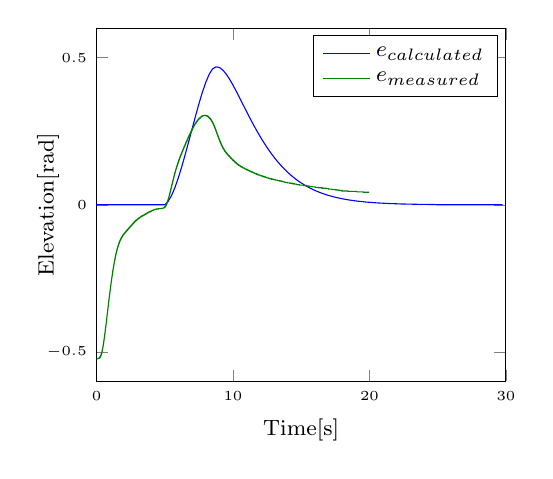
\begin{tikzpicture}

\begin{axis}[%
width = 5.2cm,
at={(0.772in,0.516in)},
scale only axis,
xmin=0,
xmax=30,
xlabel={\footnotesize{Time[s]}},
ymin=-0.6,
ymax=0.6,
ylabel={\footnotesize{Elevation[rad]}},
axis background/.style={fill=white},
ticklabel style = {font=\tiny},
ylabel shift = -0.4cm,
legend style={legend cell align=left, align=left, draw=black, font = \footnotesize}
]
\addplot [color=blue]
  table[row sep=crcr]{%
0	0\\
5	0\\
5.25	0.0111790084870798\\
5.5	0.0314285228123445\\
5.75	0.0589571543992378\\
6	0.0922242778688513\\
6.25	0.129875847906554\\
6.5	0.170685381629585\\
6.75	0.213497796741997\\
7.25	0.300541641256594\\
7.5	0.34232898323306\\
7.75	0.38111598941132\\
8	0.415265459007205\\
8.25	0.442852238150678\\
8.5	0.46158524270497\\
8.75	0.468715878925309\\
9	0.466851842459036\\
9.25	0.458129971010763\\
9.5	0.444293585959862\\
9.75	0.426757677384973\\
10	0.406662971231832\\
10.25	0.384923307218362\\
10.75	0.339254788123753\\
11.25	0.293847504952478\\
11.5	0.272037456697252\\
11.75	0.251088367331022\\
12	0.231125940976632\\
12.25	0.212230920522753\\
12.5	0.194448554601916\\
12.75	0.177795884159032\\
13	0.16226822316548\\
13.25	0.147844447077212\\
13.5	0.134491694237489\\
13.75	0.122167453715186\\
14	0.110823445674527\\
14.25	0.100407024401854\\
14.5	0.0908636264836069\\
14.75	0.0821376572517032\\
15	0.0741736887539624\\
15.25	0.0669178221019777\\
15.5	0.0603172853547704\\
15.75	0.0543215239931385\\
16	0.0488827401906597\\
16.25	0.0439552884880605\\
16.5	0.039496113114545\\
17	0.0318252011785489\\
17.5	0.025581216082383\\
18	0.0205163610018566\\
18.5	0.0164208238337658\\
19	0.0131176017427954\\
19.75	0.00933514693502246\\
20.5	0.00662072174521811\\
21.25	0.00468070626050476\\
22.25	0.00293462057759797\\
23.5	0.00162741815917045\\
24.75	0.000897979831691487\\
25	0\\
29.75	0\\
};
\addlegendentry{$e_{\text{calculated}}$}

\addplot [color=black!50!green]
  table[row sep=crcr]{%
0	-0.523598775598298\\
0.0960000000000001	-0.523598775598298\\
0.097999999999999	-0.522064794810412\\
0.193999999999999	-0.522064794810412\\
0.196000000000002	-0.520530814022528\\
0.23	-0.520530814022528\\
0.231999999999999	-0.518996833234642\\
0.257999999999999	-0.518996833234642\\
0.260000000000002	-0.517462852446755\\
0.276	-0.517462852446755\\
0.277999999999999	-0.515928871658872\\
0.295999999999999	-0.515928871658872\\
0.297999999999998	-0.514394890870985\\
0.309999999999999	-0.514394890870985\\
0.312000000000001	-0.512860910083099\\
0.324000000000002	-0.512860910083099\\
0.326000000000001	-0.511326929295215\\
0.334	-0.511326929295215\\
0.335999999999999	-0.509792948507329\\
0.346	-0.509792948507329\\
0.347999999999999	-0.508258967719442\\
0.356000000000002	-0.508258967719442\\
0.358000000000001	-0.506724986931555\\
0.366	-0.506724986931555\\
0.367999999999999	-0.505191006143672\\
0.376000000000001	-0.505191006143672\\
0.378	-0.503657025355785\\
0.384	-0.503657025355785\\
0.385999999999999	-0.502123044567899\\
0.391999999999999	-0.502123044567899\\
0.393999999999998	-0.500589063780016\\
0.399999999999999	-0.500589063780016\\
0.402000000000001	-0.499055082992129\\
0.408000000000001	-0.499055082992129\\
0.41	-0.497521102204242\\
0.414000000000001	-0.497521102204242\\
0.416	-0.495987121416356\\
0.422000000000001	-0.495987121416356\\
0.423999999999999	-0.494453140628472\\
0.428000000000001	-0.494453140628472\\
0.43	-0.492919159840586\\
0.434000000000001	-0.492919159840586\\
0.436	-0.491385179052699\\
0.442	-0.491385179052699\\
0.443999999999999	-0.489851198264816\\
0.448	-0.489851198264816\\
0.449999999999999	-0.488317217476929\\
0.454000000000001	-0.488317217476929\\
0.456	-0.486783236689043\\
0.460000000000001	-0.486783236689043\\
0.462	-0.485249255901159\\
0.466000000000001	-0.485249255901159\\
0.468	-0.483715275113273\\
0.472000000000001	-0.483715275113273\\
0.474	-0.482181294325386\\
0.478000000000002	-0.482181294325386\\
0.48	-0.480647313537499\\
0.484000000000002	-0.480647313537499\\
0.486000000000001	-0.479113332749616\\
0.489999999999998	-0.479113332749616\\
0.492000000000001	-0.47757935196173\\
0.494	-0.47757935196173\\
0.495999999999999	-0.476045371173843\\
0.5	-0.476045371173843\\
0.501999999999999	-0.47451139038596\\
0.504000000000001	-0.47451139038596\\
0.506	-0.472977409598073\\
0.510000000000002	-0.472977409598073\\
0.512	-0.471443428810186\\
0.516000000000002	-0.471443428810186\\
0.518000000000001	-0.469909448022303\\
0.52	-0.469909448022303\\
0.521999999999998	-0.468375467234416\\
0.526	-0.468375467234416\\
0.527999999999999	-0.46684148644653\\
0.530000000000001	-0.46684148644653\\
0.532	-0.465307505658643\\
0.536000000000001	-0.465307505658643\\
0.538	-0.46377352487076\\
0.539999999999999	-0.46377352487076\\
0.542000000000002	-0.462239544082873\\
0.545999999999999	-0.462239544082873\\
0.548000000000002	-0.460705563294987\\
0.550000000000001	-0.460705563294987\\
0.552	-0.459171582507103\\
0.553999999999998	-0.459171582507103\\
0.556000000000001	-0.457637601719217\\
0.559999999999999	-0.457637601719217\\
0.562000000000001	-0.45610362093133\\
0.564	-0.45610362093133\\
0.565999999999999	-0.454569640143443\\
0.568000000000001	-0.454569640143443\\
0.57	-0.45303565935556\\
0.574000000000002	-0.45303565935556\\
0.576000000000001	-0.451501678567674\\
0.577999999999999	-0.451501678567674\\
0.579999999999998	-0.449967697779787\\
0.582000000000001	-0.449967697779787\\
0.584	-0.448433716991904\\
0.585999999999999	-0.448433716991904\\
0.588000000000001	-0.446899736204017\\
0.591999999999999	-0.446899736204017\\
0.594000000000001	-0.44536575541613\\
0.596	-0.44536575541613\\
0.597999999999999	-0.443831774628247\\
0.600000000000001	-0.443831774628247\\
0.602	-0.44229779384036\\
0.603999999999999	-0.44229779384036\\
0.606000000000002	-0.440763813052474\\
0.608000000000001	-0.440763813052474\\
0.609999999999999	-0.439229832264587\\
0.611999999999998	-0.439229832264587\\
0.614000000000001	-0.437695851476704\\
0.616	-0.437695851476704\\
0.617999999999999	-0.436161870688817\\
0.622	-0.436161870688817\\
0.623999999999999	-0.434627889900931\\
0.626000000000001	-0.434627889900931\\
0.628	-0.433093909113047\\
0.629999999999999	-0.433093909113047\\
0.632000000000001	-0.431559928325161\\
0.634	-0.431559928325161\\
0.635999999999999	-0.430025947537274\\
0.638000000000002	-0.430025947537274\\
0.640000000000001	-0.428491966749387\\
0.641999999999999	-0.428491966749387\\
0.643999999999998	-0.426957985961504\\
0.646000000000001	-0.426957985961504\\
0.648	-0.425424005173618\\
0.649999999999999	-0.425424005173618\\
0.652000000000001	-0.423890024385731\\
0.655999999999999	-0.423890024385731\\
0.658000000000001	-0.422356043597848\\
0.66	-0.422356043597848\\
0.661999999999999	-0.420822062809961\\
0.664000000000001	-0.420822062809961\\
0.666	-0.419288082022074\\
0.667999999999999	-0.419288082022074\\
0.670000000000002	-0.417754101234191\\
0.672000000000001	-0.417754101234191\\
0.673999999999999	-0.416220120446305\\
0.675999999999998	-0.416220120446305\\
0.678000000000001	-0.414686139658418\\
0.68	-0.414686139658418\\
0.681999999999999	-0.413152158870531\\
0.684000000000001	-0.413152158870531\\
0.686	-0.411618178082648\\
0.687999999999999	-0.411618178082648\\
0.690000000000001	-0.410084197294761\\
0.692	-0.410084197294761\\
0.693999999999999	-0.408550216506875\\
0.696000000000002	-0.408550216506875\\
0.698	-0.407016235718991\\
0.699999999999999	-0.407016235718991\\
0.702000000000002	-0.405482254931105\\
0.704000000000001	-0.405482254931105\\
0.706	-0.403948274143218\\
0.707999999999998	-0.403948274143218\\
0.710000000000001	-0.402414293355335\\
0.712	-0.402414293355335\\
0.713999999999999	-0.400880312567448\\
0.716000000000001	-0.400880312567448\\
0.718	-0.399346331779562\\
0.719999999999999	-0.399346331779562\\
0.722000000000001	-0.397812350991675\\
0.724	-0.397812350991675\\
0.725999999999999	-0.396278370203792\\
0.728000000000002	-0.396278370203792\\
0.73	-0.394744389415905\\
0.731999999999999	-0.394744389415905\\
0.734000000000002	-0.393210408628018\\
0.736000000000001	-0.393210408628018\\
0.738	-0.391676427840135\\
0.739999999999998	-0.391676427840135\\
0.742000000000001	-0.390142447052249\\
0.744	-0.390142447052249\\
0.748000000000001	-0.387074485476475\\
0.751999999999999	-0.387074485476475\\
0.754000000000001	-0.385540504688592\\
0.756	-0.385540504688592\\
0.757999999999999	-0.384006523900705\\
0.760000000000002	-0.384006523900705\\
0.763999999999999	-0.380938562324936\\
0.766000000000002	-0.380938562324936\\
0.768000000000001	-0.379404581537049\\
0.77	-0.379404581537049\\
0.771999999999998	-0.377870600749162\\
0.774000000000001	-0.377870600749162\\
0.776	-0.376336619961279\\
0.777999999999999	-0.376336619961279\\
0.780000000000001	-0.374802639173392\\
0.782	-0.374802639173392\\
0.783999999999999	-0.373268658385506\\
0.786000000000001	-0.373268658385506\\
0.788	-0.371734677597619\\
0.789999999999999	-0.371734677597619\\
0.792000000000002	-0.370200696809736\\
0.794	-0.370200696809736\\
0.795999999999999	-0.368666716021849\\
0.798000000000002	-0.368666716021849\\
0.800000000000001	-0.367132735233962\\
0.802	-0.367132735233962\\
0.803999999999998	-0.365598754446079\\
0.806000000000001	-0.365598754446079\\
0.808	-0.364064773658193\\
0.809999999999999	-0.364064773658193\\
0.812000000000001	-0.362530792870306\\
0.814	-0.362530792870306\\
0.815999999999999	-0.360996812082419\\
0.818000000000001	-0.360996812082419\\
0.82	-0.359462831294536\\
0.821999999999999	-0.359462831294536\\
0.824000000000002	-0.357928850506649\\
0.826000000000001	-0.357928850506649\\
0.827999999999999	-0.356394869718763\\
0.830000000000002	-0.356394869718763\\
0.832000000000001	-0.35486088893088\\
0.834	-0.35486088893088\\
0.835999999999999	-0.353326908142993\\
0.838000000000001	-0.353326908142993\\
0.84	-0.351792927355106\\
0.841999999999999	-0.351792927355106\\
0.844000000000001	-0.350258946567223\\
0.846	-0.350258946567223\\
0.850000000000001	-0.34719098499145\\
0.852	-0.34719098499145\\
0.853999999999999	-0.345657004203563\\
0.856000000000002	-0.345657004203563\\
0.858000000000001	-0.34412302341568\\
0.861999999999998	-0.34412302341568\\
0.864000000000001	-0.342589042627793\\
0.866	-0.342589042627793\\
0.870000000000001	-0.339521081052023\\
0.872	-0.339521081052023\\
0.873999999999999	-0.337987100264137\\
0.876000000000001	-0.337987100264137\\
0.878	-0.33645311947625\\
0.879999999999999	-0.33645311947625\\
0.882000000000001	-0.334919138688367\\
0.884	-0.334919138688367\\
0.885999999999999	-0.33338515790048\\
0.888000000000002	-0.33338515790048\\
0.890000000000001	-0.331851177112593\\
0.891999999999999	-0.331851177112593\\
0.893999999999998	-0.330317196324707\\
0.896000000000001	-0.330317196324707\\
0.898	-0.328783215536824\\
0.899999999999999	-0.328783215536824\\
0.902000000000001	-0.327249234748937\\
0.904	-0.327249234748937\\
0.905999999999999	-0.32571525396105\\
0.908000000000001	-0.32571525396105\\
0.91	-0.324181273173167\\
0.911999999999999	-0.324181273173167\\
0.914000000000001	-0.32264729238528\\
0.916	-0.32264729238528\\
0.917999999999999	-0.321113311597394\\
0.920000000000002	-0.321113311597394\\
0.922000000000001	-0.319579330809507\\
0.923999999999999	-0.319579330809507\\
0.925999999999998	-0.318045350021624\\
0.928000000000001	-0.318045350021624\\
0.93	-0.316511369233737\\
0.931999999999999	-0.316511369233737\\
0.934000000000001	-0.31497738844585\\
0.936	-0.31497738844585\\
0.937999999999999	-0.313443407657967\\
0.940000000000001	-0.313443407657967\\
0.942	-0.311909426870081\\
0.946000000000002	-0.311909426870081\\
0.948	-0.310375446082194\\
0.949999999999999	-0.310375446082194\\
0.952000000000002	-0.308841465294311\\
0.954000000000001	-0.308841465294311\\
0.956	-0.307307484506424\\
0.957999999999998	-0.307307484506424\\
0.960000000000001	-0.305773503718537\\
0.962	-0.305773503718537\\
0.963999999999999	-0.304239522930651\\
0.966000000000001	-0.304239522930651\\
0.968	-0.302705542142768\\
0.969999999999999	-0.302705542142768\\
0.972000000000001	-0.301171561354881\\
0.974	-0.301171561354881\\
0.975999999999999	-0.299637580566994\\
0.978000000000002	-0.299637580566994\\
0.98	-0.298103599779111\\
0.981999999999999	-0.298103599779111\\
0.984000000000002	-0.296569618991224\\
0.986000000000001	-0.296569618991224\\
0.988	-0.295035638203338\\
0.992000000000001	-0.295035638203338\\
0.994	-0.293501657415451\\
0.995999999999999	-0.293501657415451\\
0.998000000000001	-0.291967676627568\\
1	-0.291967676627568\\
1.004	-0.288899715051794\\
1.008	-0.288899715051794\\
1.01	-0.287365734263911\\
1.012	-0.287365734263911\\
1.014	-0.285831753476025\\
1.016	-0.285831753476025\\
1.018	-0.284297772688138\\
1.02	-0.284297772688138\\
1.022	-0.282763791900255\\
1.024	-0.282763791900255\\
1.026	-0.281229811112368\\
1.03	-0.281229811112368\\
1.032	-0.279695830324481\\
1.034	-0.279695830324481\\
1.036	-0.278161849536595\\
1.038	-0.278161849536595\\
1.04	-0.276627868748712\\
1.042	-0.276627868748712\\
1.044	-0.275093887960825\\
1.046	-0.275093887960825\\
1.048	-0.273559907172938\\
1.052	-0.273559907172938\\
1.054	-0.272025926385055\\
1.056	-0.272025926385055\\
1.058	-0.270491945597168\\
1.06	-0.270491945597168\\
1.062	-0.268957964809282\\
1.064	-0.268957964809282\\
1.066	-0.267423984021399\\
1.068	-0.267423984021399\\
1.07	-0.265890003233512\\
1.074	-0.265890003233512\\
1.076	-0.264356022445625\\
1.078	-0.264356022445625\\
1.08	-0.262822041657738\\
1.082	-0.262822041657738\\
1.084	-0.261288060869855\\
1.086	-0.261288060869855\\
1.088	-0.259754080081969\\
1.092	-0.259754080081969\\
1.094	-0.258220099294082\\
1.096	-0.258220099294082\\
1.098	-0.256686118506199\\
1.1	-0.256686118506199\\
1.102	-0.255152137718312\\
1.106	-0.255152137718312\\
1.108	-0.253618156930425\\
1.11	-0.253618156930425\\
1.112	-0.252084176142539\\
1.114	-0.252084176142539\\
1.116	-0.250550195354656\\
1.12	-0.250550195354656\\
1.122	-0.249016214566769\\
1.124	-0.249016214566769\\
1.126	-0.247482233778882\\
1.128	-0.247482233778882\\
1.13	-0.245948252990999\\
1.134	-0.245948252990999\\
1.136	-0.244414272203112\\
1.14	-0.244414272203112\\
1.142	-0.242880291415226\\
1.144	-0.242880291415226\\
1.146	-0.241346310627343\\
1.148	-0.241346310627343\\
1.15	-0.239812329839456\\
1.154	-0.239812329839456\\
1.156	-0.238278349051569\\
1.158	-0.238278349051569\\
1.16	-0.236744368263683\\
1.164	-0.236744368263683\\
1.166	-0.235210387475799\\
1.168	-0.235210387475799\\
1.17	-0.233676406687913\\
1.172	-0.233676406687913\\
1.174	-0.232142425900026\\
1.178	-0.232142425900026\\
1.18	-0.230608445112143\\
1.184	-0.230608445112143\\
1.186	-0.229074464324256\\
1.188	-0.229074464324256\\
1.19	-0.227540483536369\\
1.192	-0.227540483536369\\
1.194	-0.226006502748483\\
1.198	-0.226006502748483\\
1.2	-0.2244725219606\\
1.204	-0.2244725219606\\
1.206	-0.222938541172713\\
1.208	-0.222938541172713\\
1.21	-0.221404560384826\\
1.214	-0.221404560384826\\
1.216	-0.219870579596943\\
1.22	-0.219870579596943\\
1.222	-0.218336598809056\\
1.224	-0.218336598809056\\
1.226	-0.21680261802117\\
1.23	-0.21680261802117\\
1.232	-0.215268637233287\\
1.236	-0.215268637233287\\
1.238	-0.2137346564454\\
1.242	-0.2137346564454\\
1.244	-0.212200675657513\\
1.246	-0.212200675657513\\
1.248	-0.210666694869627\\
1.252	-0.210666694869627\\
1.254	-0.209132714081743\\
1.258	-0.209132714081743\\
1.26	-0.207598733293857\\
1.264	-0.207598733293857\\
1.266	-0.20606475250597\\
1.27	-0.20606475250597\\
1.272	-0.204530771718087\\
1.274	-0.204530771718087\\
1.276	-0.2029967909302\\
1.28	-0.2029967909302\\
1.282	-0.201462810142313\\
1.286	-0.201462810142313\\
1.288	-0.19992882935443\\
1.292	-0.19992882935443\\
1.294	-0.198394848566544\\
1.298	-0.198394848566544\\
1.3	-0.196860867778657\\
1.304	-0.196860867778657\\
1.306	-0.19532688699077\\
1.31	-0.19532688699077\\
1.312	-0.193792906202887\\
1.316	-0.193792906202887\\
1.318	-0.192258925415\\
1.322	-0.192258925415\\
1.324	-0.190724944627114\\
1.328	-0.190724944627114\\
1.33	-0.189190963839231\\
1.334	-0.189190963839231\\
1.336	-0.187656983051344\\
1.342	-0.187656983051344\\
1.344	-0.186123002263457\\
1.348	-0.186123002263457\\
1.35	-0.184589021475571\\
1.354	-0.184589021475571\\
1.356	-0.183055040687687\\
1.36	-0.183055040687687\\
1.362	-0.181521059899801\\
1.368	-0.181521059899801\\
1.37	-0.179987079111914\\
1.374	-0.179987079111914\\
1.376	-0.178453098324031\\
1.38	-0.178453098324031\\
1.382	-0.176919117536144\\
1.388	-0.176919117536144\\
1.39	-0.175385136748258\\
1.394	-0.175385136748258\\
1.396	-0.173851155960374\\
1.402	-0.173851155960374\\
1.404	-0.172317175172488\\
1.408	-0.172317175172488\\
1.41	-0.170783194384601\\
1.416	-0.170783194384601\\
1.418	-0.169249213596714\\
1.424	-0.169249213596714\\
1.426	-0.167715232808831\\
1.43	-0.167715232808831\\
1.432	-0.166181252020944\\
1.438	-0.166181252020944\\
1.44	-0.164647271233058\\
1.446	-0.164647271233058\\
1.448	-0.163113290445175\\
1.454	-0.163113290445175\\
1.456	-0.161579309657288\\
1.462	-0.161579309657288\\
1.464	-0.160045328869401\\
1.47	-0.160045328869401\\
1.472	-0.158511348081515\\
1.478	-0.158511348081515\\
1.48	-0.156977367293631\\
1.486	-0.156977367293631\\
1.488	-0.155443386505745\\
1.494	-0.155443386505745\\
1.496	-0.153909405717858\\
1.502	-0.153909405717858\\
1.504	-0.152375424929975\\
1.512	-0.152375424929975\\
1.514	-0.150841444142088\\
1.522	-0.150841444142088\\
1.524	-0.149307463354202\\
1.53	-0.149307463354202\\
1.532	-0.147773482566318\\
1.54	-0.147773482566318\\
1.542	-0.146239501778432\\
1.548	-0.146239501778432\\
1.55	-0.144705520990545\\
1.558	-0.144705520990545\\
1.56	-0.143171540202658\\
1.568	-0.143171540202658\\
1.57	-0.141637559414775\\
1.578	-0.141637559414775\\
1.58	-0.140103578626888\\
1.588	-0.140103578626888\\
1.59	-0.138569597839002\\
1.598	-0.138569597839002\\
1.6	-0.137035617051119\\
1.608	-0.137035617051119\\
1.61	-0.135501636263232\\
1.62	-0.135501636263232\\
1.622	-0.133967655475345\\
1.632	-0.133967655475345\\
1.634	-0.132433674687462\\
1.644	-0.132433674687462\\
1.646	-0.130899693899575\\
1.656	-0.130899693899575\\
1.658	-0.129365713111689\\
1.668	-0.129365713111689\\
1.67	-0.127831732323802\\
1.68	-0.127831732323802\\
1.682	-0.126297751535919\\
1.694	-0.126297751535919\\
1.696	-0.124763770748032\\
1.706	-0.124763770748032\\
1.708	-0.123229789960146\\
1.72	-0.123229789960146\\
1.722	-0.121695809172262\\
1.736	-0.121695809172262\\
1.738	-0.120161828384376\\
1.75	-0.120161828384376\\
1.752	-0.118627847596489\\
1.766	-0.118627847596489\\
1.768	-0.117093866808602\\
1.782	-0.117093866808602\\
1.784	-0.115559886020719\\
1.798	-0.115559886020719\\
1.8	-0.114025905232833\\
1.816	-0.114025905232833\\
1.818	-0.112491924444946\\
1.832	-0.112491924444946\\
1.834	-0.110957943657063\\
1.852	-0.110957943657063\\
1.854	-0.109423962869176\\
1.872	-0.109423962869176\\
1.874	-0.107889982081289\\
1.894	-0.107889982081289\\
1.896	-0.106356001293406\\
1.914	-0.106356001293406\\
1.916	-0.104822020505519\\
1.936	-0.104822020505519\\
1.938	-0.103288039717633\\
1.958	-0.103288039717633\\
1.96	-0.101754058929746\\
1.984	-0.101754058929746\\
1.986	-0.100220078141863\\
2.008	-0.100220078141863\\
2.01	-0.0986860973539763\\
2.036	-0.0986860973539763\\
2.038	-0.0971521165660896\\
2.064	-0.0971521165660896\\
2.066	-0.0956181357782064\\
2.092	-0.0956181357782064\\
2.094	-0.0940841549903197\\
2.116	-0.0940841549903197\\
2.118	-0.0925501742024331\\
2.146	-0.0925501742024331\\
2.148	-0.0910161934145464\\
2.176	-0.0910161934145464\\
2.178	-0.0894822126266632\\
2.206	-0.0894822126266632\\
2.208	-0.0879482318387765\\
2.236	-0.0879482318387765\\
2.238	-0.0864142510508898\\
2.264	-0.0864142510508898\\
2.266	-0.0848802702630067\\
2.29	-0.0848802702630067\\
2.292	-0.08334628947512\\
2.32	-0.08334628947512\\
2.322	-0.0818123086872333\\
2.348	-0.0818123086872333\\
2.35	-0.0802783278993502\\
2.378	-0.0802783278993502\\
2.38	-0.0787443471114635\\
2.406	-0.0787443471114635\\
2.408	-0.0772103663235768\\
2.434	-0.0772103663235768\\
2.436	-0.0756763855356901\\
2.462	-0.0756763855356901\\
2.464	-0.074142404747807\\
2.492	-0.074142404747807\\
2.494	-0.0726084239599203\\
2.52	-0.0726084239599203\\
2.522	-0.0710744431720336\\
2.55	-0.0710744431720336\\
2.552	-0.0695404623841505\\
2.578	-0.0695404623841505\\
2.58	-0.0680064815962638\\
2.606	-0.0680064815962638\\
2.608	-0.0664725008083771\\
2.636	-0.0664725008083771\\
2.638	-0.0649385200204904\\
2.668	-0.0649385200204904\\
2.67	-0.0634045392326072\\
2.698	-0.0634045392326072\\
2.7	-0.0618705584447206\\
2.728	-0.0618705584447206\\
2.73	-0.0603365776568339\\
2.76	-0.0603365776568339\\
2.762	-0.0588025968689507\\
2.794	-0.0588025968689507\\
2.796	-0.057268616081064\\
2.824	-0.057268616081064\\
2.826	-0.0557346352931773\\
2.858	-0.0557346352931773\\
2.86	-0.0542006545052942\\
2.896	-0.0542006545052942\\
2.898	-0.0526666737174075\\
2.932	-0.0526666737174075\\
2.934	-0.0511326929295208\\
2.972	-0.0511326929295208\\
2.974	-0.0495987121416341\\
3.008	-0.0495987121416341\\
3.01	-0.048064731353751\\
3.052	-0.048064731353751\\
3.054	-0.0465307505658643\\
3.098	-0.0465307505658643\\
3.1	-0.0449967697779776\\
3.142	-0.0449967697779776\\
3.144	-0.0434627889900945\\
3.194	-0.0434627889900945\\
3.196	-0.0419288082022078\\
3.244	-0.0419288082022078\\
3.246	-0.0403948274143211\\
3.3	-0.0403948274143211\\
3.302	-0.038860846626438\\
3.35	-0.038860846626438\\
3.352	-0.0373268658385513\\
3.408	-0.0373268658385513\\
3.41	-0.0357928850506646\\
3.464	-0.0357928850506646\\
3.466	-0.0342589042627779\\
3.522	-0.0342589042627779\\
3.524	-0.0327249234748948\\
3.578	-0.0327249234748948\\
3.58	-0.0311909426870081\\
3.636	-0.0311909426870081\\
3.638	-0.0296569618991214\\
3.696	-0.0296569618991214\\
3.698	-0.0281229811112382\\
3.756	-0.0281229811112382\\
3.758	-0.0265890003233515\\
3.814	-0.0265890003233515\\
3.816	-0.0250550195354649\\
3.876	-0.0250550195354649\\
3.878	-0.0235210387475782\\
3.942	-0.0235210387475782\\
3.944	-0.021987057959695\\
4.008	-0.021987057959695\\
4.01	-0.0204530771718083\\
4.072	-0.0204530771718083\\
4.074	-0.0189190963839216\\
4.146	-0.0189190963839216\\
4.148	-0.0173851155960385\\
4.244	-0.0173851155960385\\
4.246	-0.0158511348081518\\
4.362	-0.0158511348081518\\
4.364	-0.0143171540202651\\
4.54	-0.0143171540202651\\
4.542	-0.012783173232382\\
4.816	-0.012783173232382\\
4.818	-0.0112491924444953\\
4.932	-0.0112491924444953\\
4.934	-0.0097152116566086\\
4.984	-0.0097152116566086\\
4.986	-0.00818123086872191\\
5.016	-0.00818123086872191\\
5.018	-0.00664725008083877\\
5.042	-0.00664725008083877\\
5.044	-0.00511326929295208\\
5.064	-0.00511326929295208\\
5.066	-0.00357928850506539\\
5.084	-0.00357928850506539\\
5.086	-0.00204530771718225\\
5.102	-0.00204530771718225\\
5.104	-0.000511326929295564\\
5.118	-0.000511326929295564\\
5.12	0.00102265385859113\\
5.132	0.00102265385859113\\
5.134	0.00255663464647782\\
5.148	0.00255663464647782\\
5.15	0.00409061543436096\\
5.16	0.00409061543436096\\
5.162	0.00562459622224765\\
5.172	0.00562459622224765\\
5.174	0.00715857701013434\\
5.184	0.00715857701013434\\
5.186	0.00869255779801748\\
5.198	0.00869255779801748\\
5.2	0.0102265385859042\\
5.208	0.0102265385859042\\
5.21	0.0117605193737909\\
5.218	0.0117605193737909\\
5.22	0.013294500161674\\
5.23	0.013294500161674\\
5.232	0.0148284809495607\\
5.24	0.0148284809495607\\
5.242	0.0163624617374474\\
5.25	0.0163624617374474\\
5.252	0.0178964425253341\\
5.26	0.0178964425253341\\
5.262	0.0194304233132172\\
5.27	0.0194304233132172\\
5.272	0.0209644041011039\\
5.278	0.0209644041011039\\
5.28	0.0224983848889906\\
5.288	0.0224983848889906\\
5.29	0.0240323656768737\\
5.298	0.0240323656768737\\
5.3	0.0255663464647604\\
5.306	0.0255663464647604\\
5.308	0.0271003272526471\\
5.316	0.0271003272526471\\
5.318	0.0286343080405302\\
5.324	0.0286343080405302\\
5.326	0.0301682888284169\\
5.332	0.0301682888284169\\
5.334	0.0317022696163036\\
5.342	0.0317022696163036\\
5.344	0.0332362504041903\\
5.35	0.0332362504041903\\
5.352	0.0347702311920735\\
5.358	0.0347702311920735\\
5.36	0.0363042119799601\\
5.368	0.0363042119799601\\
5.37	0.0378381927678468\\
5.374	0.0378381927678468\\
5.376	0.03937217355573\\
5.384	0.03937217355573\\
5.386	0.0409061543436167\\
5.392	0.0409061543436167\\
5.394	0.0424401351315034\\
5.4	0.0424401351315034\\
5.402	0.04397411591939\\
5.408	0.04397411591939\\
5.41	0.0455080967072732\\
5.416	0.0455080967072732\\
5.418	0.0470420774951599\\
5.424	0.0470420774951599\\
5.426	0.0485760582830466\\
5.432	0.0485760582830466\\
5.434	0.0501100390709297\\
5.44	0.0501100390709297\\
5.442	0.0516440198588164\\
5.448	0.0516440198588164\\
5.45	0.0531780006467031\\
5.456	0.0531780006467031\\
5.458	0.0547119814345862\\
5.464	0.0547119814345862\\
5.466	0.0562459622224729\\
5.472	0.0562459622224729\\
5.474	0.0577799430103596\\
5.482	0.0577799430103596\\
5.484	0.0593139237982463\\
5.488	0.0593139237982463\\
5.49	0.0608479045861294\\
5.496	0.0608479045861294\\
5.498	0.0623818853740161\\
5.504	0.0623818853740161\\
5.506	0.0639158661619028\\
5.512	0.0639158661619028\\
5.514	0.065449846949786\\
5.52	0.065449846949786\\
5.522	0.0669838277376726\\
5.528	0.0669838277376726\\
5.53	0.0685178085255593\\
5.536	0.0685178085255593\\
5.538	0.070051789313446\\
5.544	0.070051789313446\\
5.546	0.0715857701013292\\
5.552	0.0715857701013292\\
5.554	0.0731197508892159\\
5.562	0.0731197508892159\\
5.564	0.0746537316771025\\
5.568	0.0746537316771025\\
5.57	0.0761877124649857\\
5.578	0.0761877124649857\\
5.58	0.0777216932528724\\
5.586	0.0777216932528724\\
5.588	0.0792556740407591\\
5.594	0.0792556740407591\\
5.596	0.0807896548286422\\
5.602	0.0807896548286422\\
5.604	0.0823236356165289\\
5.61	0.0823236356165289\\
5.612	0.0838576164044156\\
5.618	0.0838576164044156\\
5.62	0.0853915971923023\\
5.626	0.0853915971923023\\
5.628	0.0869255779801854\\
5.634	0.0869255779801854\\
5.636	0.0884595587680721\\
5.644	0.0884595587680721\\
5.646	0.0899935395559588\\
5.65	0.0899935395559588\\
5.652	0.0915275203438419\\
5.66	0.0915275203438419\\
5.662	0.0930615011317286\\
5.668	0.0930615011317286\\
5.67	0.0945954819196153\\
5.676	0.0945954819196153\\
5.678	0.0961294627074984\\
5.686	0.0961294627074984\\
5.688	0.0976634434953851\\
5.694	0.0976634434953851\\
5.696	0.0991974242832718\\
5.702	0.0991974242832718\\
5.704	0.100731405071159\\
5.712	0.100731405071159\\
5.714	0.102265385859042\\
5.72	0.102265385859042\\
5.722	0.103799366646928\\
5.73	0.103799366646928\\
5.732	0.105333347434815\\
5.738	0.105333347434815\\
5.74	0.106867328222698\\
5.748	0.106867328222698\\
5.75	0.108401309010585\\
5.756	0.108401309010585\\
5.758	0.109935289798472\\
5.764	0.109935289798472\\
5.766	0.111469270586358\\
5.774	0.111469270586358\\
5.776	0.113003251374241\\
5.784	0.113003251374241\\
5.786	0.114537232162128\\
5.792	0.114537232162128\\
5.794	0.116071212950015\\
5.802	0.116071212950015\\
5.804	0.117605193737898\\
5.81	0.117605193737898\\
5.812	0.119139174525785\\
5.82	0.119139174525785\\
5.822	0.120673155313671\\
5.83	0.120673155313671\\
5.832	0.122207136101554\\
5.84	0.122207136101554\\
5.842	0.123741116889441\\
5.85	0.123741116889441\\
5.852	0.125275097677328\\
5.86	0.125275097677328\\
5.862	0.126809078465214\\
5.87	0.126809078465214\\
5.872	0.128343059253098\\
5.88	0.128343059253098\\
5.882	0.129877040040984\\
5.89	0.129877040040984\\
5.892	0.131411020828871\\
5.9	0.131411020828871\\
5.902	0.132945001616754\\
5.91	0.132945001616754\\
5.912	0.134478982404641\\
5.922	0.134478982404641\\
5.924	0.136012963192528\\
5.932	0.136012963192528\\
5.934	0.137546943980414\\
5.944	0.137546943980414\\
5.946	0.139080924768297\\
5.954	0.139080924768297\\
5.956	0.140614905556184\\
5.964	0.140614905556184\\
5.966	0.142148886344071\\
5.976	0.142148886344071\\
5.978	0.143682867131954\\
5.988	0.143682867131954\\
5.99	0.145216847919841\\
5.998	0.145216847919841\\
6	0.146750828707727\\
6.01	0.146750828707727\\
6.012	0.14828480949561\\
6.022	0.14828480949561\\
6.024	0.149818790283497\\
6.034	0.149818790283497\\
6.036	0.151352771071384\\
6.044	0.151352771071384\\
6.046	0.15288675185927\\
6.056	0.15288675185927\\
6.058	0.154420732647154\\
6.07	0.154420732647154\\
6.072	0.15595471343504\\
6.082	0.15595471343504\\
6.084	0.157488694222927\\
6.094	0.157488694222927\\
6.096	0.15902267501081\\
6.106	0.15902267501081\\
6.108	0.160556655798697\\
6.118	0.160556655798697\\
6.12	0.162090636586584\\
6.132	0.162090636586584\\
6.134	0.163624617374467\\
6.144	0.163624617374467\\
6.146	0.165158598162353\\
6.156	0.165158598162353\\
6.158	0.16669257895024\\
6.17	0.16669257895024\\
6.172	0.168226559738127\\
6.184	0.168226559738127\\
6.186	0.16976054052601\\
6.198	0.16976054052601\\
6.2	0.171294521313897\\
6.21	0.171294521313897\\
6.212	0.172828502101783\\
6.222	0.172828502101783\\
6.224	0.174362482889666\\
6.236	0.174362482889666\\
6.238	0.175896463677553\\
6.248	0.175896463677553\\
6.25	0.17743044446544\\
6.26	0.17743044446544\\
6.262	0.178964425253326\\
6.274	0.178964425253326\\
6.276	0.18049840604121\\
6.288	0.18049840604121\\
6.29	0.182032386829096\\
6.304	0.182032386829096\\
6.306	0.183566367616983\\
6.318	0.183566367616983\\
6.32	0.185100348404866\\
6.332	0.185100348404866\\
6.334	0.186634329192753\\
6.346	0.186634329192753\\
6.348	0.188168309980639\\
6.36	0.188168309980639\\
6.362	0.189702290768523\\
6.372	0.189702290768523\\
6.374	0.191236271556409\\
6.386	0.191236271556409\\
6.388	0.192770252344296\\
6.4	0.192770252344296\\
6.402	0.194304233132183\\
6.412	0.194304233132183\\
6.414	0.195838213920066\\
6.426	0.195838213920066\\
6.428	0.197372194707953\\
6.44	0.197372194707953\\
6.442	0.198906175495839\\
6.456	0.198906175495839\\
6.458	0.200440156283722\\
6.47	0.200440156283722\\
6.472	0.201974137071609\\
6.486	0.201974137071609\\
6.488	0.203508117859496\\
6.5	0.203508117859496\\
6.502	0.205042098647382\\
6.514	0.205042098647382\\
6.516	0.206576079435266\\
6.526	0.206576079435266\\
6.528	0.208110060223152\\
6.54	0.208110060223152\\
6.542	0.209644041011039\\
6.554	0.209644041011039\\
6.556	0.211178021798922\\
6.57	0.211178021798922\\
6.572	0.212712002586809\\
6.584	0.212712002586809\\
6.586	0.214245983374695\\
6.6	0.214245983374695\\
6.602	0.215779964162579\\
6.616	0.215779964162579\\
6.618	0.217313944950465\\
6.63	0.217313944950465\\
6.632	0.218847925738352\\
6.642	0.218847925738352\\
6.644	0.220381906526239\\
6.658	0.220381906526239\\
6.66	0.221915887314122\\
6.672	0.221915887314122\\
6.674	0.223449868102009\\
6.688	0.223449868102009\\
6.69	0.224983848889895\\
6.702	0.224983848889895\\
6.704	0.226517829677778\\
6.718	0.226517829677778\\
6.72	0.228051810465665\\
6.734	0.228051810465665\\
6.736	0.229585791253552\\
6.75	0.229585791253552\\
6.752	0.231119772041435\\
6.764	0.231119772041435\\
6.766	0.232653752829322\\
6.778	0.232653752829322\\
6.78	0.234187733617208\\
6.794	0.234187733617208\\
6.796	0.235721714405095\\
6.808	0.235721714405095\\
6.81	0.237255695192978\\
6.824	0.237255695192978\\
6.826	0.238789675980865\\
6.842	0.238789675980865\\
6.844	0.240323656768751\\
6.856	0.240323656768751\\
6.858	0.241857637556635\\
6.872	0.241857637556635\\
6.874	0.243391618344521\\
6.886	0.243391618344521\\
6.888	0.244925599132408\\
6.902	0.244925599132408\\
6.904	0.246459579920295\\
6.918	0.246459579920295\\
6.92	0.247993560708178\\
6.934	0.247993560708178\\
6.936	0.249527541496064\\
6.948	0.249527541496064\\
6.95	0.251061522283951\\
6.968	0.251061522283951\\
6.97	0.252595503071834\\
6.984	0.252595503071834\\
6.986	0.254129483859721\\
7	0.254129483859721\\
7.002	0.255663464647608\\
7.018	0.255663464647608\\
7.02	0.257197445435491\\
7.034	0.257197445435491\\
7.036	0.258731426223378\\
7.048	0.258731426223378\\
7.05	0.260265407011264\\
7.066	0.260265407011264\\
7.068	0.261799387799151\\
7.084	0.261799387799151\\
7.086	0.263333368587034\\
7.1	0.263333368587034\\
7.102	0.264867349374921\\
7.12	0.264867349374921\\
7.122	0.266401330162807\\
7.14	0.266401330162807\\
7.142	0.267935310950691\\
7.158	0.267935310950691\\
7.16	0.269469291738577\\
7.176	0.269469291738577\\
7.178	0.271003272526464\\
7.196	0.271003272526464\\
7.198	0.272537253314351\\
7.214	0.272537253314351\\
7.216	0.274071234102234\\
7.232	0.274071234102234\\
7.234	0.27560521489012\\
7.252	0.27560521489012\\
7.254	0.277139195678007\\
7.276	0.277139195678007\\
7.278	0.27867317646589\\
7.298	0.27867317646589\\
7.3	0.280207157253777\\
7.318	0.280207157253777\\
7.32	0.281741138041664\\
7.342	0.281741138041664\\
7.344	0.283275118829547\\
7.366	0.283275118829547\\
7.368	0.284809099617434\\
7.392	0.284809099617434\\
7.394	0.28634308040532\\
7.416	0.28634308040532\\
7.418	0.287877061193207\\
7.442	0.287877061193207\\
7.444	0.28941104198109\\
7.468	0.28941104198109\\
7.47	0.290945022768977\\
7.504	0.290945022768977\\
7.506	0.292479003556863\\
7.532	0.292479003556863\\
7.534	0.294012984344747\\
7.568	0.294012984344747\\
7.57	0.295546965132633\\
7.604	0.295546965132633\\
7.606	0.29708094592052\\
7.644	0.29708094592052\\
7.646	0.298614926708407\\
7.686	0.298614926708407\\
7.688	0.30014890749629\\
7.736	0.30014890749629\\
7.738	0.301682888284176\\
7.798	0.301682888284176\\
7.8	0.303216869072063\\
7.948	0.303216869072063\\
7.95	0.304750849859946\\
7.952	0.304750849859946\\
7.954	0.303216869072063\\
7.962	0.303216869072063\\
7.964	0.304750849859946\\
7.966	0.303216869072063\\
8.074	0.303216869072063\\
8.076	0.301682888284176\\
8.08	0.301682888284176\\
8.082	0.303216869072063\\
8.086	0.303216869072063\\
8.088	0.301682888284176\\
8.146	0.301682888284176\\
8.148	0.30014890749629\\
8.194	0.30014890749629\\
8.196	0.298614926708407\\
8.222	0.298614926708407\\
8.224	0.29708094592052\\
8.226	0.29708094592052\\
8.228	0.298614926708407\\
8.23	0.298614926708407\\
8.232	0.29708094592052\\
8.258	0.29708094592052\\
8.26	0.295546965132633\\
8.292	0.295546965132633\\
8.294	0.294012984344747\\
8.32	0.294012984344747\\
8.322	0.292479003556863\\
8.344	0.292479003556863\\
8.346	0.290945022768977\\
8.37	0.290945022768977\\
8.372	0.28941104198109\\
8.392	0.28941104198109\\
8.394	0.287877061193207\\
8.414	0.287877061193207\\
8.416	0.28634308040532\\
8.436	0.28634308040532\\
8.438	0.284809099617434\\
8.454	0.284809099617434\\
8.456	0.283275118829547\\
8.476	0.283275118829547\\
8.478	0.281741138041664\\
8.492	0.281741138041664\\
8.494	0.280207157253777\\
8.508	0.280207157253777\\
8.51	0.27867317646589\\
8.528	0.27867317646589\\
8.53	0.277139195678007\\
8.542	0.277139195678007\\
8.544	0.27560521489012\\
8.558	0.27560521489012\\
8.56	0.274071234102234\\
8.572	0.274071234102234\\
8.574	0.272537253314351\\
8.586	0.272537253314351\\
8.588	0.271003272526464\\
8.602	0.271003272526464\\
8.604	0.269469291738577\\
8.616	0.269469291738577\\
8.618	0.267935310950691\\
8.63	0.267935310950691\\
8.632	0.266401330162807\\
8.644	0.266401330162807\\
8.646	0.264867349374921\\
8.658	0.264867349374921\\
8.66	0.263333368587034\\
8.672	0.263333368587034\\
8.674	0.261799387799151\\
8.684	0.261799387799151\\
8.686	0.260265407011264\\
8.698	0.260265407011264\\
8.7	0.258731426223378\\
8.71	0.258731426223378\\
8.712	0.257197445435491\\
8.722	0.257197445435491\\
8.724	0.255663464647608\\
8.734	0.255663464647608\\
8.736	0.254129483859721\\
8.746	0.254129483859721\\
8.748	0.252595503071834\\
8.758	0.252595503071834\\
8.76	0.251061522283951\\
8.77	0.251061522283951\\
8.772	0.249527541496064\\
8.782	0.249527541496064\\
8.784	0.247993560708178\\
8.794	0.247993560708178\\
8.796	0.246459579920295\\
8.804	0.246459579920295\\
8.806	0.244925599132408\\
8.818	0.244925599132408\\
8.82	0.243391618344521\\
8.828	0.243391618344521\\
8.83	0.241857637556635\\
8.842	0.241857637556635\\
8.844	0.240323656768751\\
8.854	0.240323656768751\\
8.856	0.238789675980865\\
8.866	0.238789675980865\\
8.868	0.237255695192978\\
8.878	0.237255695192978\\
8.88	0.235721714405095\\
8.89	0.235721714405095\\
8.892	0.234187733617208\\
8.902	0.234187733617208\\
8.904	0.232653752829322\\
8.914	0.232653752829322\\
8.916	0.231119772041435\\
8.926	0.231119772041435\\
8.928	0.229585791253552\\
8.938	0.229585791253552\\
8.94	0.228051810465665\\
8.952	0.228051810465665\\
8.954	0.226517829677778\\
8.964	0.226517829677778\\
8.966	0.224983848889895\\
8.976	0.224983848889895\\
8.978	0.223449868102009\\
8.988	0.223449868102009\\
8.99	0.221915887314122\\
9.002	0.221915887314122\\
9.004	0.220381906526239\\
9.014	0.220381906526239\\
9.016	0.218847925738352\\
9.026	0.218847925738352\\
9.028	0.217313944950465\\
9.04	0.217313944950465\\
9.042	0.215779964162579\\
9.054	0.215779964162579\\
9.056	0.214245983374695\\
9.068	0.214245983374695\\
9.07	0.212712002586809\\
9.08	0.212712002586809\\
9.082	0.211178021798922\\
9.094	0.211178021798922\\
9.096	0.209644041011039\\
9.108	0.209644041011039\\
9.11	0.208110060223152\\
9.124	0.208110060223152\\
9.126	0.206576079435266\\
9.138	0.206576079435266\\
9.14	0.205042098647382\\
9.154	0.205042098647382\\
9.156	0.203508117859496\\
9.168	0.203508117859496\\
9.17	0.201974137071609\\
9.186	0.201974137071609\\
9.188	0.200440156283722\\
9.202	0.200440156283722\\
9.204	0.198906175495839\\
9.216	0.198906175495839\\
9.218	0.197372194707953\\
9.23	0.197372194707953\\
9.232	0.195838213920066\\
9.252	0.195838213920066\\
9.254	0.194304233132183\\
9.266	0.194304233132183\\
9.268	0.192770252344296\\
9.288	0.192770252344296\\
9.29	0.191236271556409\\
9.304	0.191236271556409\\
9.306	0.189702290768523\\
9.326	0.189702290768523\\
9.328	0.188168309980639\\
9.346	0.188168309980639\\
9.348	0.186634329192753\\
9.366	0.186634329192753\\
9.368	0.185100348404866\\
9.388	0.185100348404866\\
9.39	0.183566367616983\\
9.412	0.183566367616983\\
9.414	0.182032386829096\\
9.432	0.182032386829096\\
9.434	0.18049840604121\\
9.458	0.18049840604121\\
9.46	0.178964425253326\\
9.482	0.178964425253326\\
9.484	0.17743044446544\\
9.508	0.17743044446544\\
9.51	0.175896463677553\\
9.532	0.175896463677553\\
9.534	0.174362482889666\\
9.56	0.174362482889666\\
9.562	0.172828502101783\\
9.59	0.172828502101783\\
9.592	0.171294521313897\\
9.62	0.171294521313897\\
9.622	0.16976054052601\\
9.646	0.16976054052601\\
9.648	0.168226559738127\\
9.678	0.168226559738127\\
9.68	0.16669257895024\\
9.71	0.16669257895024\\
9.712	0.165158598162353\\
9.738	0.165158598162353\\
9.74	0.163624617374467\\
9.768	0.163624617374467\\
9.77	0.162090636586584\\
9.804	0.162090636586584\\
9.806	0.160556655798697\\
9.834	0.160556655798697\\
9.836	0.15902267501081\\
9.866	0.15902267501081\\
9.868	0.157488694222927\\
9.894	0.157488694222927\\
9.896	0.15595471343504\\
9.934	0.15595471343504\\
9.936	0.154420732647154\\
9.972	0.154420732647154\\
9.974	0.15288675185927\\
9.996	0.15288675185927\\
9.998	0.151352771071384\\
10.024	0.151352771071384\\
10.026	0.149818790283497\\
10.07	0.149818790283497\\
10.072	0.14828480949561\\
10.108	0.14828480949561\\
10.11	0.146750828707727\\
10.134	0.146750828707727\\
10.136	0.145216847919841\\
10.162	0.145216847919841\\
10.164	0.143682867131954\\
10.224	0.143682867131954\\
10.226	0.142148886344071\\
10.256	0.142148886344071\\
10.258	0.140614905556184\\
10.282	0.140614905556184\\
10.284	0.139080924768297\\
10.322	0.139080924768297\\
10.324	0.137546943980414\\
10.386	0.137546943980414\\
10.388	0.136012963192528\\
10.414	0.136012963192528\\
10.416	0.134478982404641\\
10.456	0.134478982404641\\
10.458	0.132945001616754\\
10.524	0.132945001616754\\
10.526	0.131411020828871\\
10.564	0.131411020828871\\
10.566	0.129877040040984\\
10.614	0.129877040040984\\
10.616	0.128343059253098\\
10.684	0.128343059253098\\
10.686	0.126809078465214\\
10.724	0.126809078465214\\
10.726	0.125275097677328\\
10.812	0.125275097677328\\
10.814	0.123741116889441\\
10.856	0.123741116889441\\
10.858	0.122207136101554\\
10.942	0.122207136101554\\
10.944	0.120673155313671\\
10.992	0.120673155313671\\
10.994	0.119139174525785\\
11.064	0.119139174525785\\
11.066	0.117605193737898\\
11.134	0.117605193737898\\
11.136	0.116071212950015\\
11.196	0.116071212950015\\
11.198	0.114537232162128\\
11.278	0.114537232162128\\
11.28	0.113003251374241\\
11.344	0.113003251374241\\
11.346	0.111469270586358\\
11.422	0.111469270586358\\
11.424	0.109935289798472\\
11.494	0.109935289798472\\
11.496	0.108401309010585\\
11.57	0.108401309010585\\
11.572	0.106867328222698\\
11.66	0.106867328222698\\
11.662	0.105333347434815\\
11.728	0.105333347434815\\
11.73	0.103799366646928\\
11.828	0.103799366646928\\
11.83	0.102265385859042\\
11.892	0.102265385859042\\
11.894	0.100731405071159\\
11.994	0.100731405071159\\
11.996	0.0991974242832718\\
12.09	0.0991974242832718\\
12.092	0.0976634434953851\\
12.174	0.0976634434953851\\
12.176	0.0961294627074984\\
12.29	0.0961294627074984\\
12.292	0.0945954819196153\\
12.396	0.0945954819196153\\
12.398	0.0930615011317286\\
12.49	0.0930615011317286\\
12.492	0.0915275203438419\\
12.6	0.0915275203438419\\
12.602	0.0899935395559588\\
12.712	0.0899935395559588\\
12.714	0.0884595587680721\\
12.826	0.0884595587680721\\
12.828	0.0869255779801854\\
12.952	0.0869255779801854\\
12.954	0.0853915971923023\\
13.09	0.0853915971923023\\
13.092	0.0838576164044156\\
13.258	0.0838576164044156\\
13.26	0.0823236356165289\\
13.414	0.0823236356165289\\
13.416	0.0807896548286422\\
13.554	0.0807896548286422\\
13.556	0.0792556740407591\\
13.68	0.0792556740407591\\
13.682	0.0777216932528724\\
13.808	0.0777216932528724\\
13.81	0.0761877124649857\\
13.974	0.0761877124649857\\
13.976	0.0746537316771025\\
14.168	0.0746537316771025\\
14.17	0.0731197508892159\\
14.348	0.0731197508892159\\
14.35	0.0715857701013292\\
14.488	0.0715857701013292\\
14.49	0.070051789313446\\
14.642	0.070051789313446\\
14.644	0.0685178085255593\\
14.866	0.0685178085255593\\
14.868	0.0669838277376726\\
15.172	0.0669838277376726\\
15.174	0.065449846949786\\
15.368	0.065449846949786\\
15.37	0.0639158661619028\\
15.564	0.0639158661619028\\
15.566	0.0623818853740161\\
15.804	0.0623818853740161\\
15.806	0.0608479045861294\\
16.032	0.0608479045861294\\
16.034	0.0593139237982463\\
16.272	0.0593139237982463\\
16.274	0.0577799430103596\\
16.538	0.0577799430103596\\
16.54	0.0562459622224729\\
16.806	0.0562459622224729\\
16.808	0.0547119814345862\\
17.012	0.0547119814345862\\
17.014	0.0531780006467031\\
17.268	0.0531780006467031\\
17.27	0.0516440198588164\\
17.548	0.0516440198588164\\
17.55	0.0501100390709297\\
17.76	0.0501100390709297\\
17.762	0.0485760582830466\\
17.988	0.0485760582830466\\
17.99	0.0470420774951599\\
18.426	0.0470420774951599\\
18.428	0.0455080967072732\\
19.08	0.0455080967072732\\
19.082	0.04397411591939\\
19.55	0.04397411591939\\
19.552	0.0424401351315034\\
19.98	0.0424401351315034\\
};
\addlegendentry{$e_{\text{measured}}$}

\end{axis}
\end{tikzpicture}%

        \phantomcaption
        \label{fig:4_worst_elevation}
    \end{subfigure}%
    ~
    \begin{subfigure}[t]{0.5\textwidth}
        \centering
        % This file was created by matlab2tikz.
%
%The latest updates can be retrieved from
%  http://www.mathworks.com/matlabcentral/fileexchange/22022-matlab2tikz-matlab2tikz
%where you can also make suggestions and rate matlab2tikz.
%
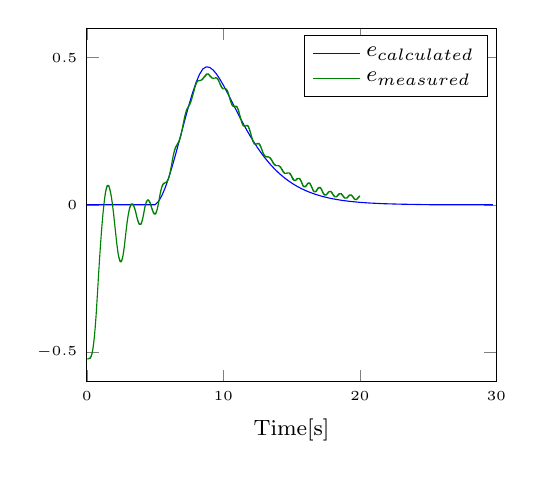
\begin{tikzpicture}

\begin{axis}[%
width = 5.2cm,
at={(0.758in,0.488in)},
scale only axis,
xmin=0,
xmax=30,
xlabel={\footnotesize{Time[s]}},
ymin=-0.6,
ymax=0.6,
axis background/.style={fill=white},
ticklabel style = {font=\tiny},
legend style={legend cell align=left, align=left, draw=black, font = \footnotesize}
]
\addplot [color=blue]
  table[row sep=crcr]{%
0	0\\
5	0\\
5.25	0.0111790084870798\\
5.5	0.0314285228123445\\
5.75	0.0589571543992378\\
6	0.0922242778688513\\
6.25	0.129875847906554\\
6.5	0.170685381629585\\
6.75	0.213497796741997\\
7.25	0.300541641256594\\
7.5	0.34232898323306\\
7.75	0.38111598941132\\
8	0.415265459007205\\
8.25	0.442852238150678\\
8.5	0.46158524270497\\
8.75	0.468715878925309\\
9	0.466851842459036\\
9.25	0.458129971010763\\
9.5	0.444293585959862\\
9.75	0.426757677384973\\
10	0.406662971231832\\
10.25	0.384923307218362\\
10.75	0.339254788123753\\
11.25	0.293847504952478\\
11.5	0.272037456697252\\
11.75	0.251088367331022\\
12	0.231125940976632\\
12.25	0.212230920522753\\
12.5	0.194448554601916\\
12.75	0.177795884159032\\
13	0.16226822316548\\
13.25	0.147844447077212\\
13.5	0.134491694237489\\
13.75	0.122167453715186\\
14	0.110823445674527\\
14.25	0.100407024401854\\
14.5	0.0908636264836069\\
14.75	0.0821376572517032\\
15	0.0741736887539624\\
15.25	0.0669178221019777\\
15.5	0.0603172853547704\\
15.75	0.0543215239931385\\
16	0.0488827401906597\\
16.25	0.0439552884880605\\
16.75	0.0354651938147548\\
17.25	0.0285412354643277\\
17.75	0.0229153425454278\\
18.25	0.0183591876706615\\
18.75	0.0146800138948002\\
19.25	0.0117162649150906\\
20	0.00832798453404848\\
20.75	0.00590001772599535\\
21.75	0.00370831938445448\\
23	0.00206173375537944\\
25.5	0\\
29.75	0\\
};
\addlegendentry{$e_{\text{calculated}}$}

\addplot [color=black!50!green]
  table[row sep=crcr]{%
0	-0.523598775598298\\
0.154	-0.523598775598298\\
0.155999999999999	-0.522064794810412\\
0.218	-0.522064794810412\\
0.219999999999999	-0.520530814022528\\
0.25	-0.520530814022528\\
0.251999999999999	-0.518996833234642\\
0.274000000000001	-0.518996833234642\\
0.276	-0.517462852446755\\
0.292000000000002	-0.517462852446755\\
0.294	-0.515928871658872\\
0.308	-0.515928871658872\\
0.309999999999999	-0.514394890870985\\
0.321999999999999	-0.514394890870985\\
0.324000000000002	-0.512860910083099\\
0.332000000000001	-0.512860910083099\\
0.334	-0.511326929295215\\
0.344000000000001	-0.511326929295215\\
0.346	-0.509792948507329\\
0.353999999999999	-0.509792948507329\\
0.356000000000002	-0.508258967719442\\
0.364000000000001	-0.508258967719442\\
0.366	-0.506724986931555\\
0.372	-0.506724986931555\\
0.373999999999999	-0.505191006143672\\
0.379999999999999	-0.505191006143672\\
0.382000000000001	-0.503657025355785\\
0.388000000000002	-0.503657025355785\\
0.390000000000001	-0.502123044567899\\
0.396000000000001	-0.502123044567899\\
0.398	-0.500589063780016\\
0.402000000000001	-0.500589063780016\\
0.404	-0.499055082992129\\
0.41	-0.499055082992129\\
0.411999999999999	-0.497521102204242\\
0.416	-0.497521102204242\\
0.417999999999999	-0.495987121416356\\
0.422000000000001	-0.495987121416356\\
0.423999999999999	-0.494453140628472\\
0.428000000000001	-0.494453140628472\\
0.43	-0.492919159840586\\
0.434000000000001	-0.492919159840586\\
0.436	-0.491385179052699\\
0.437999999999999	-0.491385179052699\\
0.440000000000001	-0.489851198264816\\
0.443999999999999	-0.489851198264816\\
0.446000000000002	-0.488317217476929\\
0.449999999999999	-0.488317217476929\\
0.452000000000002	-0.486783236689043\\
0.454000000000001	-0.486783236689043\\
0.456	-0.485249255901159\\
0.460000000000001	-0.485249255901159\\
0.462	-0.483715275113273\\
0.463999999999999	-0.483715275113273\\
0.466000000000001	-0.482181294325386\\
0.468	-0.482181294325386\\
0.469999999999999	-0.480647313537499\\
0.474	-0.480647313537499\\
0.475999999999999	-0.479113332749616\\
0.478000000000002	-0.479113332749616\\
0.48	-0.47757935196173\\
0.481999999999999	-0.47757935196173\\
0.484000000000002	-0.476045371173843\\
0.486000000000001	-0.476045371173843\\
0.488	-0.47451139038596\\
0.489999999999998	-0.47451139038596\\
0.492000000000001	-0.472977409598073\\
0.494	-0.472977409598073\\
0.495999999999999	-0.471443428810186\\
0.5	-0.471443428810186\\
0.504000000000001	-0.468375467234416\\
0.506	-0.468375467234416\\
0.507999999999999	-0.46684148644653\\
0.510000000000002	-0.46684148644653\\
0.512	-0.465307505658643\\
0.513999999999999	-0.465307505658643\\
0.516000000000002	-0.46377352487076\\
0.518000000000001	-0.46377352487076\\
0.52	-0.462239544082873\\
0.521999999999998	-0.462239544082873\\
0.526	-0.459171582507103\\
0.527999999999999	-0.459171582507103\\
0.530000000000001	-0.457637601719217\\
0.532	-0.457637601719217\\
0.533999999999999	-0.45610362093133\\
0.536000000000001	-0.45610362093133\\
0.539999999999999	-0.45303565935556\\
0.542000000000002	-0.45303565935556\\
0.544	-0.451501678567674\\
0.545999999999999	-0.451501678567674\\
0.550000000000001	-0.448433716991904\\
0.552	-0.448433716991904\\
0.556000000000001	-0.44536575541613\\
0.558	-0.44536575541613\\
0.559999999999999	-0.443831774628247\\
0.562000000000001	-0.443831774628247\\
0.565999999999999	-0.440763813052474\\
0.568000000000001	-0.440763813052474\\
0.571999999999999	-0.437695851476704\\
0.574000000000002	-0.437695851476704\\
0.577999999999999	-0.434627889900931\\
0.579999999999998	-0.434627889900931\\
0.584	-0.431559928325161\\
0.585999999999999	-0.431559928325161\\
0.591999999999999	-0.426957985961504\\
0.594000000000001	-0.426957985961504\\
0.597999999999999	-0.423890024385731\\
0.600000000000001	-0.423890024385731\\
0.603999999999999	-0.420822062809961\\
0.606000000000002	-0.420822062809961\\
0.611999999999998	-0.416220120446305\\
0.614000000000001	-0.416220120446305\\
0.622	-0.410084197294761\\
0.623999999999999	-0.410084197294761\\
0.632000000000001	-0.403948274143218\\
0.634	-0.403948274143218\\
0.643999999999998	-0.396278370203792\\
0.646000000000001	-0.396278370203792\\
0.654	-0.390142447052249\\
0.655999999999999	-0.390142447052249\\
0.666	-0.382472543112819\\
0.667999999999999	-0.382472543112819\\
0.686	-0.368666716021849\\
0.687999999999999	-0.368666716021849\\
0.718	-0.345657004203563\\
0.719999999999999	-0.345657004203563\\
0.722000000000001	-0.34412302341568\\
0.724	-0.341055061839906\\
0.728000000000002	-0.337987100264137\\
0.73	-0.337987100264137\\
0.734000000000002	-0.334919138688367\\
0.736000000000001	-0.331851177112593\\
0.738	-0.330317196324707\\
0.739999999999998	-0.330317196324707\\
0.744	-0.327249234748937\\
0.745999999999999	-0.324181273173167\\
0.748000000000001	-0.324181273173167\\
0.824000000000002	-0.265890003233512\\
0.826000000000001	-0.262822041657738\\
0.884	-0.218336598809056\\
0.885999999999999	-0.218336598809056\\
0.93	-0.184589021475571\\
0.931999999999999	-0.184589021475571\\
0.954000000000001	-0.167715232808831\\
0.956	-0.167715232808831\\
0.975999999999999	-0.152375424929975\\
0.978000000000002	-0.152375424929975\\
0.992000000000001	-0.141637559414775\\
0.994	-0.141637559414775\\
1.008	-0.130899693899575\\
1.01	-0.130899693899575\\
1.022	-0.121695809172262\\
1.024	-0.121695809172262\\
1.034	-0.114025905232833\\
1.036	-0.114025905232833\\
1.046	-0.106356001293406\\
1.048	-0.106356001293406\\
1.056	-0.100220078141863\\
1.058	-0.100220078141863\\
1.066	-0.0940841549903197\\
1.068	-0.0940841549903197\\
1.076	-0.0879482318387765\\
1.078	-0.0879482318387765\\
1.084	-0.08334628947512\\
1.086	-0.08334628947512\\
1.092	-0.0787443471114635\\
1.094	-0.0787443471114635\\
1.1	-0.074142404747807\\
1.102	-0.074142404747807\\
1.108	-0.0695404623841505\\
1.11	-0.0695404623841505\\
1.116	-0.0649385200204904\\
1.118	-0.0649385200204904\\
1.124	-0.0603365776568339\\
1.126	-0.0603365776568339\\
1.13	-0.057268616081064\\
1.132	-0.057268616081064\\
1.138	-0.0526666737174075\\
1.14	-0.0526666737174075\\
1.144	-0.0495987121416341\\
1.146	-0.0495987121416341\\
1.15	-0.0465307505658643\\
1.152	-0.0465307505658643\\
1.158	-0.0419288082022078\\
1.16	-0.0419288082022078\\
1.164	-0.038860846626438\\
1.166	-0.038860846626438\\
1.17	-0.0357928850506646\\
1.172	-0.0357928850506646\\
1.176	-0.0327249234748948\\
1.178	-0.0327249234748948\\
1.18	-0.0311909426870081\\
1.182	-0.0311909426870081\\
1.186	-0.0281229811112382\\
1.188	-0.0281229811112382\\
1.192	-0.0250550195354649\\
1.194	-0.0250550195354649\\
1.198	-0.021987057959695\\
1.2	-0.021987057959695\\
1.202	-0.0204530771718083\\
1.204	-0.0204530771718083\\
1.208	-0.0173851155960385\\
1.21	-0.0173851155960385\\
1.212	-0.0158511348081518\\
1.214	-0.0158511348081518\\
1.218	-0.012783173232382\\
1.22	-0.012783173232382\\
1.222	-0.0112491924444953\\
1.224	-0.0112491924444953\\
1.226	-0.0097152116566086\\
1.228	-0.0097152116566086\\
1.232	-0.00664725008083877\\
1.234	-0.00664725008083877\\
1.236	-0.00511326929295208\\
1.238	-0.00511326929295208\\
1.242	-0.00204530771718225\\
1.244	-0.00204530771718225\\
1.246	-0.000511326929295564\\
1.248	-0.000511326929295564\\
1.25	0.00102265385859113\\
1.252	0.00102265385859113\\
1.254	0.00255663464647782\\
1.256	0.00255663464647782\\
1.258	0.00409061543436096\\
1.26	0.00409061543436096\\
1.262	0.00562459622224765\\
1.264	0.00562459622224765\\
1.268	0.00869255779801748\\
1.27	0.00869255779801748\\
1.272	0.0102265385859042\\
1.274	0.0102265385859042\\
1.276	0.0117605193737909\\
1.278	0.0117605193737909\\
1.28	0.013294500161674\\
1.282	0.013294500161674\\
1.284	0.0148284809495607\\
1.286	0.0148284809495607\\
1.288	0.0163624617374474\\
1.29	0.0163624617374474\\
1.292	0.0178964425253341\\
1.294	0.0178964425253341\\
1.296	0.0194304233132172\\
1.298	0.0194304233132172\\
1.3	0.0209644041011039\\
1.302	0.0209644041011039\\
1.304	0.0224983848889906\\
1.308	0.0224983848889906\\
1.31	0.0240323656768737\\
1.312	0.0240323656768737\\
1.314	0.0255663464647604\\
1.316	0.0255663464647604\\
1.318	0.0271003272526471\\
1.32	0.0271003272526471\\
1.322	0.0286343080405302\\
1.326	0.0286343080405302\\
1.328	0.0301682888284169\\
1.33	0.0301682888284169\\
1.332	0.0317022696163036\\
1.336	0.0317022696163036\\
1.338	0.0332362504041903\\
1.34	0.0332362504041903\\
1.342	0.0347702311920735\\
1.346	0.0347702311920735\\
1.348	0.0363042119799601\\
1.35	0.0363042119799601\\
1.352	0.0378381927678468\\
1.356	0.0378381927678468\\
1.358	0.03937217355573\\
1.362	0.03937217355573\\
1.364	0.0409061543436167\\
1.368	0.0409061543436167\\
1.37	0.0424401351315034\\
1.374	0.0424401351315034\\
1.376	0.04397411591939\\
1.38	0.04397411591939\\
1.382	0.0455080967072732\\
1.386	0.0455080967072732\\
1.388	0.0470420774951599\\
1.394	0.0470420774951599\\
1.396	0.0485760582830466\\
1.4	0.0485760582830466\\
1.402	0.0501100390709297\\
1.406	0.0501100390709297\\
1.408	0.0516440198588164\\
1.414	0.0516440198588164\\
1.416	0.0531780006467031\\
1.42	0.0531780006467031\\
1.422	0.0547119814345862\\
1.43	0.0547119814345862\\
1.432	0.0562459622224729\\
1.438	0.0562459622224729\\
1.44	0.0577799430103596\\
1.448	0.0577799430103596\\
1.45	0.0593139237982463\\
1.458	0.0593139237982463\\
1.46	0.0608479045861294\\
1.47	0.0608479045861294\\
1.472	0.0623818853740161\\
1.484	0.0623818853740161\\
1.486	0.0639158661619028\\
1.506	0.0639158661619028\\
1.508	0.065449846949786\\
1.51	0.065449846949786\\
1.512	0.0639158661619028\\
1.516	0.0639158661619028\\
1.518	0.065449846949786\\
1.586	0.065449846949786\\
1.588	0.0639158661619028\\
1.61	0.0639158661619028\\
1.612	0.0623818853740161\\
1.626	0.0623818853740161\\
1.628	0.0608479045861294\\
1.636	0.0608479045861294\\
1.638	0.0593139237982463\\
1.646	0.0593139237982463\\
1.648	0.0577799430103596\\
1.656	0.0577799430103596\\
1.658	0.0562459622224729\\
1.666	0.0562459622224729\\
1.668	0.0547119814345862\\
1.674	0.0547119814345862\\
1.676	0.0531780006467031\\
1.684	0.0531780006467031\\
1.686	0.0516440198588164\\
1.69	0.0516440198588164\\
1.692	0.0501100390709297\\
1.7	0.0501100390709297\\
1.702	0.0485760582830466\\
1.708	0.0485760582830466\\
1.71	0.0470420774951599\\
1.716	0.0470420774951599\\
1.718	0.0455080967072732\\
1.724	0.0455080967072732\\
1.726	0.04397411591939\\
1.732	0.04397411591939\\
1.734	0.0424401351315034\\
1.738	0.0424401351315034\\
1.74	0.0409061543436167\\
1.746	0.0409061543436167\\
1.748	0.03937217355573\\
1.752	0.03937217355573\\
1.754	0.0378381927678468\\
1.758	0.0378381927678468\\
1.76	0.0363042119799601\\
1.764	0.0363042119799601\\
1.766	0.0347702311920735\\
1.77	0.0347702311920735\\
1.772	0.0332362504041903\\
1.776	0.0332362504041903\\
1.778	0.0317022696163036\\
1.782	0.0317022696163036\\
1.784	0.0301682888284169\\
1.786	0.0301682888284169\\
1.788	0.0286343080405302\\
1.792	0.0286343080405302\\
1.794	0.0271003272526471\\
1.798	0.0271003272526471\\
1.8	0.0255663464647604\\
1.802	0.0255663464647604\\
1.804	0.0240323656768737\\
1.808	0.0240323656768737\\
1.81	0.0224983848889906\\
1.812	0.0224983848889906\\
1.814	0.0209644041011039\\
1.818	0.0209644041011039\\
1.82	0.0194304233132172\\
1.822	0.0194304233132172\\
1.824	0.0178964425253341\\
1.826	0.0178964425253341\\
1.828	0.0163624617374474\\
1.832	0.0163624617374474\\
1.834	0.0148284809495607\\
1.836	0.0148284809495607\\
1.838	0.013294500161674\\
1.842	0.013294500161674\\
1.844	0.0117605193737909\\
1.846	0.0117605193737909\\
1.848	0.0102265385859042\\
1.85	0.0102265385859042\\
1.852	0.00869255779801748\\
1.856	0.00869255779801748\\
1.858	0.00715857701013434\\
1.86	0.00715857701013434\\
1.862	0.00562459622224765\\
1.864	0.00562459622224765\\
1.866	0.00409061543436096\\
1.87	0.00409061543436096\\
1.872	0.00255663464647782\\
1.874	0.00255663464647782\\
1.876	0.00102265385859113\\
1.878	0.00102265385859113\\
1.88	-0.000511326929295564\\
1.882	-0.000511326929295564\\
1.884	-0.00204530771718225\\
1.886	-0.00204530771718225\\
1.888	-0.00357928850506539\\
1.89	-0.00357928850506539\\
1.892	-0.00511326929295208\\
1.896	-0.00511326929295208\\
1.898	-0.00664725008083877\\
1.9	-0.00664725008083877\\
1.902	-0.00818123086872191\\
1.904	-0.00818123086872191\\
1.906	-0.0097152116566086\\
1.908	-0.0097152116566086\\
1.91	-0.0112491924444953\\
1.912	-0.0112491924444953\\
1.914	-0.012783173232382\\
1.916	-0.012783173232382\\
1.918	-0.0143171540202651\\
1.92	-0.0143171540202651\\
1.922	-0.0158511348081518\\
1.924	-0.0158511348081518\\
1.926	-0.0173851155960385\\
1.928	-0.0173851155960385\\
1.93	-0.0189190963839216\\
1.932	-0.0189190963839216\\
1.934	-0.0204530771718083\\
1.936	-0.0204530771718083\\
1.938	-0.021987057959695\\
1.94	-0.021987057959695\\
1.942	-0.0235210387475782\\
1.944	-0.0235210387475782\\
1.946	-0.0250550195354649\\
1.948	-0.0250550195354649\\
1.952	-0.0281229811112382\\
1.954	-0.0281229811112382\\
1.956	-0.0296569618991214\\
1.958	-0.0296569618991214\\
1.96	-0.0311909426870081\\
1.962	-0.0311909426870081\\
1.964	-0.0327249234748948\\
1.966	-0.0327249234748948\\
1.968	-0.0342589042627779\\
1.97	-0.0342589042627779\\
1.974	-0.0373268658385513\\
1.976	-0.0373268658385513\\
1.978	-0.038860846626438\\
1.98	-0.038860846626438\\
1.982	-0.0403948274143211\\
1.984	-0.0403948274143211\\
1.986	-0.0419288082022078\\
1.988	-0.0419288082022078\\
1.992	-0.0449967697779776\\
1.994	-0.0449967697779776\\
1.996	-0.0465307505658643\\
1.998	-0.0465307505658643\\
2	-0.048064731353751\\
2.002	-0.048064731353751\\
2.006	-0.0511326929295208\\
2.008	-0.0511326929295208\\
2.01	-0.0526666737174075\\
2.012	-0.0526666737174075\\
2.014	-0.0542006545052942\\
2.016	-0.0542006545052942\\
2.018	-0.0557346352931773\\
2.02	-0.0557346352931773\\
2.024	-0.0588025968689507\\
2.026	-0.0588025968689507\\
2.028	-0.0603365776568339\\
2.03	-0.0603365776568339\\
2.032	-0.0618705584447206\\
2.034	-0.0618705584447206\\
2.038	-0.0649385200204904\\
2.04	-0.0649385200204904\\
2.042	-0.0664725008083771\\
2.044	-0.0664725008083771\\
2.046	-0.0680064815962638\\
2.048	-0.0680064815962638\\
2.052	-0.0710744431720336\\
2.054	-0.0710744431720336\\
2.056	-0.0726084239599203\\
2.058	-0.0726084239599203\\
2.06	-0.074142404747807\\
2.062	-0.074142404747807\\
2.066	-0.0772103663235768\\
2.068	-0.0772103663235768\\
2.07	-0.0787443471114635\\
2.072	-0.0787443471114635\\
2.076	-0.0818123086872333\\
2.078	-0.0818123086872333\\
2.08	-0.08334628947512\\
2.082	-0.08334628947512\\
2.084	-0.0848802702630067\\
2.086	-0.0848802702630067\\
2.09	-0.0879482318387765\\
2.092	-0.0879482318387765\\
2.094	-0.0894822126266632\\
2.096	-0.0894822126266632\\
2.098	-0.0910161934145464\\
2.1	-0.0910161934145464\\
2.104	-0.0940841549903197\\
2.106	-0.0940841549903197\\
2.108	-0.0956181357782064\\
2.11	-0.0956181357782064\\
2.112	-0.0971521165660896\\
2.114	-0.0971521165660896\\
2.118	-0.100220078141863\\
2.12	-0.100220078141863\\
2.122	-0.101754058929746\\
2.124	-0.101754058929746\\
2.126	-0.103288039717633\\
2.128	-0.103288039717633\\
2.132	-0.106356001293406\\
2.134	-0.106356001293406\\
2.136	-0.107889982081289\\
2.138	-0.107889982081289\\
2.14	-0.109423962869176\\
2.142	-0.109423962869176\\
2.146	-0.112491924444946\\
2.148	-0.112491924444946\\
2.15	-0.114025905232833\\
2.152	-0.114025905232833\\
2.154	-0.115559886020719\\
2.156	-0.115559886020719\\
2.158	-0.117093866808602\\
2.16	-0.117093866808602\\
2.162	-0.118627847596489\\
2.164	-0.118627847596489\\
2.166	-0.120161828384376\\
2.168	-0.120161828384376\\
2.17	-0.121695809172262\\
2.172	-0.121695809172262\\
2.176	-0.124763770748032\\
2.178	-0.124763770748032\\
2.18	-0.126297751535919\\
2.182	-0.126297751535919\\
2.184	-0.127831732323802\\
2.186	-0.127831732323802\\
2.188	-0.129365713111689\\
2.19	-0.129365713111689\\
2.192	-0.130899693899575\\
2.194	-0.130899693899575\\
2.196	-0.132433674687462\\
2.198	-0.132433674687462\\
2.2	-0.133967655475345\\
2.202	-0.133967655475345\\
2.204	-0.135501636263232\\
2.206	-0.135501636263232\\
2.208	-0.137035617051119\\
2.21	-0.137035617051119\\
2.212	-0.138569597839002\\
2.214	-0.138569597839002\\
2.216	-0.140103578626888\\
2.218	-0.140103578626888\\
2.22	-0.141637559414775\\
2.222	-0.141637559414775\\
2.224	-0.143171540202658\\
2.226	-0.143171540202658\\
2.228	-0.144705520990545\\
2.23	-0.144705520990545\\
2.232	-0.146239501778432\\
2.236	-0.146239501778432\\
2.238	-0.147773482566318\\
2.24	-0.147773482566318\\
2.242	-0.149307463354202\\
2.244	-0.149307463354202\\
2.246	-0.150841444142088\\
2.248	-0.150841444142088\\
2.25	-0.152375424929975\\
2.252	-0.152375424929975\\
2.254	-0.153909405717858\\
2.258	-0.153909405717858\\
2.26	-0.155443386505745\\
2.262	-0.155443386505745\\
2.264	-0.156977367293631\\
2.266	-0.156977367293631\\
2.268	-0.158511348081515\\
2.272	-0.158511348081515\\
2.274	-0.160045328869401\\
2.276	-0.160045328869401\\
2.278	-0.161579309657288\\
2.282	-0.161579309657288\\
2.284	-0.163113290445175\\
2.288	-0.163113290445175\\
2.29	-0.164647271233058\\
2.292	-0.164647271233058\\
2.294	-0.166181252020944\\
2.298	-0.166181252020944\\
2.3	-0.167715232808831\\
2.304	-0.167715232808831\\
2.306	-0.169249213596714\\
2.308	-0.169249213596714\\
2.31	-0.170783194384601\\
2.316	-0.170783194384601\\
2.318	-0.172317175172488\\
2.322	-0.172317175172488\\
2.324	-0.173851155960374\\
2.33	-0.173851155960374\\
2.332	-0.175385136748258\\
2.338	-0.175385136748258\\
2.34	-0.176919117536144\\
2.346	-0.176919117536144\\
2.348	-0.178453098324031\\
2.352	-0.178453098324031\\
2.354	-0.179987079111914\\
2.36	-0.179987079111914\\
2.362	-0.181521059899801\\
2.368	-0.181521059899801\\
2.37	-0.183055040687687\\
2.376	-0.183055040687687\\
2.378	-0.184589021475571\\
2.386	-0.184589021475571\\
2.388	-0.186123002263457\\
2.398	-0.186123002263457\\
2.4	-0.187656983051344\\
2.408	-0.187656983051344\\
2.41	-0.189190963839231\\
2.42	-0.189190963839231\\
2.422	-0.190724944627114\\
2.432	-0.190724944627114\\
2.434	-0.192258925415\\
2.464	-0.192258925415\\
2.466	-0.193792906202887\\
2.468	-0.193792906202887\\
2.47	-0.192258925415\\
2.472	-0.192258925415\\
2.474	-0.193792906202887\\
2.478	-0.193792906202887\\
2.48	-0.192258925415\\
2.484	-0.192258925415\\
2.486	-0.193792906202887\\
2.488	-0.193792906202887\\
2.49	-0.192258925415\\
2.494	-0.192258925415\\
2.496	-0.193792906202887\\
2.498	-0.193792906202887\\
2.5	-0.192258925415\\
2.52	-0.192258925415\\
2.522	-0.190724944627114\\
2.54	-0.190724944627114\\
2.542	-0.189190963839231\\
2.56	-0.189190963839231\\
2.562	-0.187656983051344\\
2.57	-0.187656983051344\\
2.572	-0.186123002263457\\
2.582	-0.186123002263457\\
2.584	-0.184589021475571\\
2.592	-0.184589021475571\\
2.594	-0.183055040687687\\
2.602	-0.183055040687687\\
2.604	-0.181521059899801\\
2.612	-0.181521059899801\\
2.614	-0.179987079111914\\
2.62	-0.179987079111914\\
2.622	-0.178453098324031\\
2.624	-0.178453098324031\\
2.626	-0.176919117536144\\
2.628	-0.178453098324031\\
2.63	-0.176919117536144\\
2.632	-0.176919117536144\\
2.634	-0.175385136748258\\
2.64	-0.175385136748258\\
2.642	-0.173851155960374\\
2.644	-0.173851155960374\\
2.646	-0.172317175172488\\
2.65	-0.172317175172488\\
2.652	-0.170783194384601\\
2.654	-0.170783194384601\\
2.656	-0.169249213596714\\
2.662	-0.169249213596714\\
2.664	-0.167715232808831\\
2.668	-0.167715232808831\\
2.67	-0.166181252020944\\
2.672	-0.166181252020944\\
2.674	-0.164647271233058\\
2.68	-0.164647271233058\\
2.684	-0.161579309657288\\
2.69	-0.161579309657288\\
2.694	-0.158511348081515\\
2.7	-0.158511348081515\\
2.704	-0.155443386505745\\
2.708	-0.155443386505745\\
2.71	-0.153909405717858\\
2.712	-0.153909405717858\\
2.714	-0.152375424929975\\
2.716	-0.152375424929975\\
2.718	-0.150841444142088\\
2.722	-0.150841444142088\\
2.726	-0.147773482566318\\
2.732	-0.147773482566318\\
2.736	-0.144705520990545\\
2.74	-0.144705520990545\\
2.742	-0.143171540202658\\
2.744	-0.143171540202658\\
2.748	-0.140103578626888\\
2.752	-0.140103578626888\\
2.756	-0.137035617051119\\
2.76	-0.137035617051119\\
2.762	-0.135501636263232\\
2.764	-0.135501636263232\\
2.768	-0.132433674687462\\
2.772	-0.132433674687462\\
2.776	-0.129365713111689\\
2.778	-0.129365713111689\\
2.78	-0.127831732323802\\
2.782	-0.127831732323802\\
2.784	-0.126297751535919\\
2.786	-0.126297751535919\\
2.788	-0.124763770748032\\
2.79	-0.124763770748032\\
2.792	-0.123229789960146\\
2.794	-0.123229789960146\\
2.798	-0.120161828384376\\
2.802	-0.120161828384376\\
2.806	-0.117093866808602\\
2.808	-0.117093866808602\\
2.81	-0.115559886020719\\
2.812	-0.115559886020719\\
2.814	-0.114025905232833\\
2.816	-0.114025905232833\\
2.82	-0.110957943657063\\
2.822	-0.110957943657063\\
2.824	-0.109423962869176\\
2.826	-0.109423962869176\\
2.828	-0.107889982081289\\
2.83	-0.107889982081289\\
2.832	-0.106356001293406\\
2.834	-0.106356001293406\\
2.836	-0.104822020505519\\
2.838	-0.104822020505519\\
2.842	-0.101754058929746\\
2.844	-0.101754058929746\\
2.846	-0.100220078141863\\
2.848	-0.100220078141863\\
2.85	-0.0986860973539763\\
2.852	-0.0986860973539763\\
2.854	-0.0971521165660896\\
2.856	-0.0971521165660896\\
2.86	-0.0940841549903197\\
2.864	-0.0940841549903197\\
2.868	-0.0910161934145464\\
2.87	-0.0910161934145464\\
2.872	-0.0894822126266632\\
2.874	-0.0894822126266632\\
2.876	-0.0879482318387765\\
2.878	-0.0879482318387765\\
2.88	-0.0864142510508898\\
2.882	-0.0864142510508898\\
2.884	-0.0848802702630067\\
2.886	-0.0848802702630067\\
2.888	-0.08334628947512\\
2.89	-0.08334628947512\\
2.892	-0.0818123086872333\\
2.894	-0.0818123086872333\\
2.896	-0.0802783278993502\\
2.898	-0.0802783278993502\\
2.9	-0.0787443471114635\\
2.902	-0.0787443471114635\\
2.904	-0.0772103663235768\\
2.906	-0.0772103663235768\\
2.908	-0.0756763855356901\\
2.91	-0.0756763855356901\\
2.912	-0.074142404747807\\
2.914	-0.074142404747807\\
2.916	-0.0726084239599203\\
2.918	-0.0726084239599203\\
2.92	-0.0710744431720336\\
2.922	-0.0710744431720336\\
2.924	-0.0695404623841505\\
2.926	-0.0695404623841505\\
2.928	-0.0680064815962638\\
2.93	-0.0680064815962638\\
2.932	-0.0664725008083771\\
2.934	-0.0664725008083771\\
2.936	-0.0649385200204904\\
2.938	-0.0649385200204904\\
2.94	-0.0634045392326072\\
2.942	-0.0634045392326072\\
2.944	-0.0618705584447206\\
2.948	-0.0618705584447206\\
2.95	-0.0603365776568339\\
2.952	-0.0603365776568339\\
2.954	-0.0588025968689507\\
2.956	-0.0588025968689507\\
2.958	-0.057268616081064\\
2.96	-0.057268616081064\\
2.962	-0.0557346352931773\\
2.966	-0.0557346352931773\\
2.968	-0.0542006545052942\\
2.97	-0.0542006545052942\\
2.972	-0.0526666737174075\\
2.974	-0.0526666737174075\\
2.976	-0.0511326929295208\\
2.98	-0.0511326929295208\\
2.982	-0.0495987121416341\\
2.984	-0.0495987121416341\\
2.986	-0.048064731353751\\
2.988	-0.048064731353751\\
2.99	-0.0465307505658643\\
2.994	-0.0465307505658643\\
2.996	-0.0449967697779776\\
2.998	-0.0449967697779776\\
3	-0.0434627889900945\\
3.004	-0.0434627889900945\\
3.006	-0.0419288082022078\\
3.008	-0.0419288082022078\\
3.01	-0.0403948274143211\\
3.014	-0.0403948274143211\\
3.016	-0.038860846626438\\
3.02	-0.038860846626438\\
3.022	-0.0373268658385513\\
3.026	-0.0373268658385513\\
3.028	-0.0357928850506646\\
3.03	-0.0357928850506646\\
3.032	-0.0342589042627779\\
3.036	-0.0342589042627779\\
3.038	-0.0327249234748948\\
3.042	-0.0327249234748948\\
3.044	-0.0311909426870081\\
3.048	-0.0311909426870081\\
3.05	-0.0296569618991214\\
3.054	-0.0296569618991214\\
3.056	-0.0281229811112382\\
3.06	-0.0281229811112382\\
3.062	-0.0265890003233515\\
3.066	-0.0265890003233515\\
3.068	-0.0250550195354649\\
3.072	-0.0250550195354649\\
3.074	-0.0235210387475782\\
3.08	-0.0235210387475782\\
3.082	-0.021987057959695\\
3.086	-0.021987057959695\\
3.088	-0.0204530771718083\\
3.094	-0.0204530771718083\\
3.096	-0.0189190963839216\\
3.1	-0.0189190963839216\\
3.102	-0.0173851155960385\\
3.108	-0.0173851155960385\\
3.11	-0.0158511348081518\\
3.116	-0.0158511348081518\\
3.118	-0.0143171540202651\\
3.124	-0.0143171540202651\\
3.126	-0.012783173232382\\
3.132	-0.012783173232382\\
3.134	-0.0112491924444953\\
3.142	-0.0112491924444953\\
3.144	-0.0097152116566086\\
3.152	-0.0097152116566086\\
3.154	-0.00818123086872191\\
3.164	-0.00818123086872191\\
3.166	-0.00664725008083877\\
3.174	-0.00664725008083877\\
3.176	-0.00511326929295208\\
3.188	-0.00511326929295208\\
3.19	-0.00357928850506539\\
3.2	-0.00357928850506539\\
3.202	-0.00204530771718225\\
3.216	-0.00204530771718225\\
3.218	-0.000511326929295564\\
3.232	-0.000511326929295564\\
3.234	0.00102265385859113\\
3.254	0.00102265385859113\\
3.256	0.00255663464647782\\
3.368	0.00255663464647782\\
3.37	0.00102265385859113\\
3.398	0.00102265385859113\\
3.4	-0.000511326929295564\\
3.416	-0.000511326929295564\\
3.418	-0.00204530771718225\\
3.432	-0.00204530771718225\\
3.434	-0.00357928850506539\\
3.446	-0.00357928850506539\\
3.448	-0.00511326929295208\\
3.46	-0.00511326929295208\\
3.462	-0.00664725008083877\\
3.47	-0.00664725008083877\\
3.472	-0.00818123086872191\\
3.482	-0.00818123086872191\\
3.484	-0.0097152116566086\\
3.49	-0.0097152116566086\\
3.492	-0.0112491924444953\\
3.5	-0.0112491924444953\\
3.502	-0.012783173232382\\
3.51	-0.012783173232382\\
3.512	-0.0143171540202651\\
3.522	-0.0143171540202651\\
3.524	-0.0158511348081518\\
3.53	-0.0158511348081518\\
3.532	-0.0173851155960385\\
3.54	-0.0173851155960385\\
3.542	-0.0189190963839216\\
3.548	-0.0189190963839216\\
3.55	-0.0204530771718083\\
3.558	-0.0204530771718083\\
3.56	-0.021987057959695\\
3.568	-0.021987057959695\\
3.57	-0.0235210387475782\\
3.576	-0.0235210387475782\\
3.578	-0.0250550195354649\\
3.584	-0.0250550195354649\\
3.586	-0.0265890003233515\\
3.592	-0.0265890003233515\\
3.594	-0.0281229811112382\\
3.6	-0.0281229811112382\\
3.602	-0.0296569618991214\\
3.608	-0.0296569618991214\\
3.61	-0.0311909426870081\\
3.614	-0.0311909426870081\\
3.616	-0.0327249234748948\\
3.622	-0.0327249234748948\\
3.624	-0.0342589042627779\\
3.63	-0.0342589042627779\\
3.632	-0.0357928850506646\\
3.638	-0.0357928850506646\\
3.64	-0.0373268658385513\\
3.646	-0.0373268658385513\\
3.648	-0.038860846626438\\
3.654	-0.038860846626438\\
3.656	-0.0403948274143211\\
3.662	-0.0403948274143211\\
3.664	-0.0419288082022078\\
3.67	-0.0419288082022078\\
3.672	-0.0434627889900945\\
3.68	-0.0434627889900945\\
3.682	-0.0449967697779776\\
3.69	-0.0449967697779776\\
3.692	-0.0465307505658643\\
3.698	-0.0465307505658643\\
3.7	-0.048064731353751\\
3.708	-0.048064731353751\\
3.71	-0.0495987121416341\\
3.716	-0.0495987121416341\\
3.718	-0.0511326929295208\\
3.726	-0.0511326929295208\\
3.728	-0.0526666737174075\\
3.736	-0.0526666737174075\\
3.738	-0.0542006545052942\\
3.746	-0.0542006545052942\\
3.748	-0.0557346352931773\\
3.756	-0.0557346352931773\\
3.758	-0.057268616081064\\
3.768	-0.057268616081064\\
3.77	-0.0588025968689507\\
3.78	-0.0588025968689507\\
3.782	-0.0603365776568339\\
3.792	-0.0603365776568339\\
3.794	-0.0618705584447206\\
3.808	-0.0618705584447206\\
3.81	-0.0634045392326072\\
3.824	-0.0634045392326072\\
3.826	-0.0649385200204904\\
3.846	-0.0649385200204904\\
3.848	-0.0664725008083771\\
3.946	-0.0664725008083771\\
3.948	-0.0649385200204904\\
3.95	-0.0649385200204904\\
3.952	-0.0664725008083771\\
3.954	-0.0664725008083771\\
3.956	-0.0649385200204904\\
3.976	-0.0649385200204904\\
3.978	-0.0634045392326072\\
3.99	-0.0634045392326072\\
3.992	-0.0618705584447206\\
3.994	-0.0634045392326072\\
3.996	-0.0618705584447206\\
4.006	-0.0618705584447206\\
4.008	-0.0603365776568339\\
4.018	-0.0603365776568339\\
4.02	-0.0588025968689507\\
4.028	-0.0588025968689507\\
4.03	-0.057268616081064\\
4.038	-0.057268616081064\\
4.04	-0.0557346352931773\\
4.048	-0.0557346352931773\\
4.05	-0.0542006545052942\\
4.056	-0.0542006545052942\\
4.058	-0.0526666737174075\\
4.066	-0.0526666737174075\\
4.068	-0.0511326929295208\\
4.072	-0.0511326929295208\\
4.074	-0.0495987121416341\\
4.08	-0.0495987121416341\\
4.082	-0.048064731353751\\
4.088	-0.048064731353751\\
4.09	-0.0465307505658643\\
4.096	-0.0465307505658643\\
4.098	-0.0449967697779776\\
4.102	-0.0449967697779776\\
4.104	-0.0434627889900945\\
4.11	-0.0434627889900945\\
4.112	-0.0419288082022078\\
4.116	-0.0419288082022078\\
4.118	-0.0403948274143211\\
4.122	-0.0403948274143211\\
4.124	-0.038860846626438\\
4.13	-0.038860846626438\\
4.132	-0.0373268658385513\\
4.136	-0.0373268658385513\\
4.138	-0.0357928850506646\\
4.142	-0.0357928850506646\\
4.144	-0.0342589042627779\\
4.15	-0.0342589042627779\\
4.152	-0.0327249234748948\\
4.156	-0.0327249234748948\\
4.158	-0.0311909426870081\\
4.162	-0.0311909426870081\\
4.164	-0.0296569618991214\\
4.168	-0.0296569618991214\\
4.17	-0.0281229811112382\\
4.174	-0.0281229811112382\\
4.176	-0.0265890003233515\\
4.18	-0.0265890003233515\\
4.182	-0.0250550195354649\\
4.186	-0.0250550195354649\\
4.188	-0.0235210387475782\\
4.192	-0.0235210387475782\\
4.194	-0.021987057959695\\
4.198	-0.021987057959695\\
4.2	-0.0204530771718083\\
4.204	-0.0204530771718083\\
4.206	-0.0189190963839216\\
4.21	-0.0189190963839216\\
4.212	-0.0173851155960385\\
4.216	-0.0173851155960385\\
4.218	-0.0158511348081518\\
4.224	-0.0158511348081518\\
4.226	-0.0143171540202651\\
4.23	-0.0143171540202651\\
4.232	-0.012783173232382\\
4.236	-0.012783173232382\\
4.238	-0.0112491924444953\\
4.244	-0.0112491924444953\\
4.246	-0.0097152116566086\\
4.25	-0.0097152116566086\\
4.252	-0.00818123086872191\\
4.258	-0.00818123086872191\\
4.26	-0.00664725008083877\\
4.266	-0.00664725008083877\\
4.268	-0.00511326929295208\\
4.274	-0.00511326929295208\\
4.276	-0.00357928850506539\\
4.282	-0.00357928850506539\\
4.284	-0.00204530771718225\\
4.29	-0.00204530771718225\\
4.292	-0.000511326929295564\\
4.3	-0.000511326929295564\\
4.302	0.00102265385859113\\
4.308	0.00102265385859113\\
4.31	0.00255663464647782\\
4.318	0.00255663464647782\\
4.32	0.00409061543436096\\
4.328	0.00409061543436096\\
4.33	0.00562459622224765\\
4.338	0.00562459622224765\\
4.34	0.00715857701013434\\
4.35	0.00715857701013434\\
4.352	0.00869255779801748\\
4.364	0.00869255779801748\\
4.366	0.0102265385859042\\
4.378	0.0102265385859042\\
4.38	0.0117605193737909\\
4.394	0.0117605193737909\\
4.396	0.013294500161674\\
4.416	0.013294500161674\\
4.418	0.0148284809495607\\
4.458	0.0148284809495607\\
4.46	0.0163624617374474\\
4.506	0.0163624617374474\\
4.508	0.0148284809495607\\
4.544	0.0148284809495607\\
4.546	0.013294500161674\\
4.568	0.013294500161674\\
4.57	0.0117605193737909\\
4.586	0.0117605193737909\\
4.588	0.0102265385859042\\
4.604	0.0102265385859042\\
4.606	0.00869255779801748\\
4.618	0.00869255779801748\\
4.62	0.00715857701013434\\
4.63	0.00715857701013434\\
4.632	0.00562459622224765\\
4.644	0.00562459622224765\\
4.646	0.00409061543436096\\
4.656	0.00409061543436096\\
4.658	0.00255663464647782\\
4.668	0.00255663464647782\\
4.67	0.00102265385859113\\
4.678	0.00102265385859113\\
4.68	-0.000511326929295564\\
4.69	-0.000511326929295564\\
4.692	-0.00204530771718225\\
4.7	-0.00204530771718225\\
4.702	-0.00357928850506539\\
4.712	-0.00357928850506539\\
4.714	-0.00511326929295208\\
4.722	-0.00511326929295208\\
4.724	-0.00664725008083877\\
4.732	-0.00664725008083877\\
4.734	-0.00818123086872191\\
4.742	-0.00818123086872191\\
4.744	-0.0097152116566086\\
4.752	-0.0097152116566086\\
4.754	-0.0112491924444953\\
4.764	-0.0112491924444953\\
4.766	-0.012783173232382\\
4.772	-0.012783173232382\\
4.774	-0.0143171540202651\\
4.784	-0.0143171540202651\\
4.786	-0.0158511348081518\\
4.796	-0.0158511348081518\\
4.798	-0.0173851155960385\\
4.808	-0.0173851155960385\\
4.81	-0.0189190963839216\\
4.82	-0.0189190963839216\\
4.822	-0.0204530771718083\\
4.832	-0.0204530771718083\\
4.834	-0.021987057959695\\
4.844	-0.021987057959695\\
4.846	-0.0235210387475782\\
4.858	-0.0235210387475782\\
4.86	-0.0250550195354649\\
4.87	-0.0250550195354649\\
4.872	-0.0265890003233515\\
4.89	-0.0265890003233515\\
4.892	-0.0281229811112382\\
4.91	-0.0281229811112382\\
4.912	-0.0296569618991214\\
4.944	-0.0296569618991214\\
4.946	-0.0311909426870081\\
5.018	-0.0311909426870081\\
5.02	-0.0296569618991214\\
5.048	-0.0296569618991214\\
5.05	-0.0281229811112382\\
5.068	-0.0281229811112382\\
5.07	-0.0265890003233515\\
5.082	-0.0265890003233515\\
5.084	-0.0250550195354649\\
5.092	-0.0250550195354649\\
5.094	-0.0235210387475782\\
5.104	-0.0235210387475782\\
5.106	-0.021987057959695\\
5.114	-0.021987057959695\\
5.116	-0.0204530771718083\\
5.124	-0.0204530771718083\\
5.126	-0.0189190963839216\\
5.134	-0.0189190963839216\\
5.136	-0.0173851155960385\\
5.144	-0.0173851155960385\\
5.146	-0.0158511348081518\\
5.152	-0.0158511348081518\\
5.154	-0.0143171540202651\\
5.162	-0.0143171540202651\\
5.164	-0.012783173232382\\
5.168	-0.012783173232382\\
5.17	-0.0112491924444953\\
5.176	-0.0112491924444953\\
5.178	-0.0097152116566086\\
5.184	-0.0097152116566086\\
5.186	-0.00818123086872191\\
5.192	-0.00818123086872191\\
5.194	-0.00664725008083877\\
5.198	-0.00664725008083877\\
5.2	-0.00511326929295208\\
5.206	-0.00511326929295208\\
5.208	-0.00357928850506539\\
5.212	-0.00357928850506539\\
5.214	-0.00204530771718225\\
5.22	-0.00204530771718225\\
5.222	-0.000511326929295564\\
5.226	-0.000511326929295564\\
5.228	0.00102265385859113\\
5.232	0.00102265385859113\\
5.234	0.00255663464647782\\
5.238	0.00255663464647782\\
5.24	0.00409061543436096\\
5.246	0.00409061543436096\\
5.248	0.00562459622224765\\
5.25	0.00562459622224765\\
5.252	0.00715857701013434\\
5.256	0.00715857701013434\\
5.258	0.00869255779801748\\
5.262	0.00869255779801748\\
5.264	0.0102265385859042\\
5.268	0.0102265385859042\\
5.27	0.0117605193737909\\
5.274	0.0117605193737909\\
5.276	0.013294500161674\\
5.28	0.013294500161674\\
5.282	0.0148284809495607\\
5.288	0.0148284809495607\\
5.29	0.0163624617374474\\
5.292	0.0163624617374474\\
5.294	0.0178964425253341\\
5.298	0.0178964425253341\\
5.3	0.0194304233132172\\
5.304	0.0194304233132172\\
5.306	0.0209644041011039\\
5.31	0.0209644041011039\\
5.312	0.0224983848889906\\
5.316	0.0224983848889906\\
5.318	0.0240323656768737\\
5.322	0.0240323656768737\\
5.324	0.0255663464647604\\
5.328	0.0255663464647604\\
5.33	0.0271003272526471\\
5.334	0.0271003272526471\\
5.336	0.0286343080405302\\
5.34	0.0286343080405302\\
5.342	0.0301682888284169\\
5.348	0.0301682888284169\\
5.35	0.0317022696163036\\
5.352	0.0317022696163036\\
5.354	0.0332362504041903\\
5.36	0.0332362504041903\\
5.362	0.0347702311920735\\
5.366	0.0347702311920735\\
5.368	0.0363042119799601\\
5.372	0.0363042119799601\\
5.374	0.0378381927678468\\
5.378	0.0378381927678468\\
5.38	0.03937217355573\\
5.386	0.03937217355573\\
5.388	0.0409061543436167\\
5.392	0.0409061543436167\\
5.394	0.0424401351315034\\
5.398	0.0424401351315034\\
5.4	0.04397411591939\\
5.406	0.04397411591939\\
5.408	0.0455080967072732\\
5.414	0.0455080967072732\\
5.416	0.0470420774951599\\
5.42	0.0470420774951599\\
5.422	0.0485760582830466\\
5.428	0.0485760582830466\\
5.43	0.0501100390709297\\
5.436	0.0501100390709297\\
5.438	0.0516440198588164\\
5.444	0.0516440198588164\\
5.446	0.0531780006467031\\
5.454	0.0531780006467031\\
5.456	0.0547119814345862\\
5.462	0.0547119814345862\\
5.464	0.0562459622224729\\
5.472	0.0562459622224729\\
5.474	0.0577799430103596\\
5.482	0.0577799430103596\\
5.484	0.0593139237982463\\
5.492	0.0593139237982463\\
5.494	0.0608479045861294\\
5.504	0.0608479045861294\\
5.506	0.0623818853740161\\
5.516	0.0623818853740161\\
5.518	0.0639158661619028\\
5.528	0.0639158661619028\\
5.53	0.065449846949786\\
5.544	0.065449846949786\\
5.546	0.0669838277376726\\
5.56	0.0669838277376726\\
5.562	0.0685178085255593\\
5.578	0.0685178085255593\\
5.58	0.070051789313446\\
5.602	0.070051789313446\\
5.604	0.0715857701013292\\
5.638	0.0715857701013292\\
5.64	0.0731197508892159\\
5.684	0.0731197508892159\\
5.686	0.0746537316771025\\
5.764	0.0746537316771025\\
5.766	0.0761877124649857\\
5.822	0.0761877124649857\\
5.824	0.0777216932528724\\
5.856	0.0777216932528724\\
5.858	0.0792556740407591\\
5.88	0.0792556740407591\\
5.882	0.0807896548286422\\
5.902	0.0807896548286422\\
5.904	0.0823236356165289\\
5.922	0.0823236356165289\\
5.924	0.0838576164044156\\
5.94	0.0838576164044156\\
5.942	0.0853915971923023\\
5.954	0.0853915971923023\\
5.956	0.0869255779801854\\
5.966	0.0869255779801854\\
5.968	0.0884595587680721\\
5.978	0.0884595587680721\\
5.98	0.0899935395559588\\
5.99	0.0899935395559588\\
5.992	0.0915275203438419\\
6.002	0.0915275203438419\\
6.004	0.0930615011317286\\
6.012	0.0930615011317286\\
6.014	0.0945954819196153\\
6.022	0.0945954819196153\\
6.024	0.0961294627074984\\
6.03	0.0961294627074984\\
6.032	0.0976634434953851\\
6.04	0.0976634434953851\\
6.042	0.0991974242832718\\
6.048	0.0991974242832718\\
6.05	0.100731405071159\\
6.058	0.100731405071159\\
6.06	0.102265385859042\\
6.066	0.102265385859042\\
6.068	0.103799366646928\\
6.072	0.103799366646928\\
6.074	0.105333347434815\\
6.082	0.105333347434815\\
6.084	0.106867328222698\\
6.088	0.106867328222698\\
6.09	0.108401309010585\\
6.096	0.108401309010585\\
6.098	0.109935289798472\\
6.104	0.109935289798472\\
6.106	0.111469270586358\\
6.11	0.111469270586358\\
6.112	0.113003251374241\\
6.116	0.113003251374241\\
6.118	0.114537232162128\\
6.124	0.114537232162128\\
6.126	0.116071212950015\\
6.13	0.116071212950015\\
6.132	0.117605193737898\\
6.138	0.117605193737898\\
6.14	0.119139174525785\\
6.144	0.119139174525785\\
6.146	0.120673155313671\\
6.15	0.120673155313671\\
6.152	0.122207136101554\\
6.158	0.122207136101554\\
6.16	0.123741116889441\\
6.162	0.123741116889441\\
6.164	0.125275097677328\\
6.17	0.125275097677328\\
6.172	0.126809078465214\\
6.176	0.126809078465214\\
6.178	0.128343059253098\\
6.18	0.128343059253098\\
6.182	0.129877040040984\\
6.188	0.129877040040984\\
6.19	0.131411020828871\\
6.192	0.131411020828871\\
6.194	0.132945001616754\\
6.2	0.132945001616754\\
6.202	0.134478982404641\\
6.204	0.134478982404641\\
6.206	0.136012963192528\\
6.212	0.136012963192528\\
6.214	0.137546943980414\\
6.218	0.137546943980414\\
6.22	0.139080924768297\\
6.224	0.139080924768297\\
6.226	0.140614905556184\\
6.23	0.140614905556184\\
6.232	0.142148886344071\\
6.234	0.142148886344071\\
6.236	0.143682867131954\\
6.242	0.143682867131954\\
6.244	0.145216847919841\\
6.248	0.145216847919841\\
6.25	0.146750828707727\\
6.252	0.146750828707727\\
6.254	0.14828480949561\\
6.258	0.14828480949561\\
6.26	0.149818790283497\\
6.264	0.149818790283497\\
6.266	0.151352771071384\\
6.27	0.151352771071384\\
6.272	0.15288675185927\\
6.276	0.15288675185927\\
6.278	0.154420732647154\\
6.284	0.154420732647154\\
6.286	0.15595471343504\\
6.288	0.15595471343504\\
6.29	0.157488694222927\\
6.296	0.157488694222927\\
6.298	0.15902267501081\\
6.302	0.15902267501081\\
6.304	0.160556655798697\\
6.308	0.160556655798697\\
6.31	0.162090636586584\\
6.314	0.162090636586584\\
6.316	0.163624617374467\\
6.322	0.163624617374467\\
6.324	0.165158598162353\\
6.328	0.165158598162353\\
6.33	0.16669257895024\\
6.334	0.16669257895024\\
6.336	0.168226559738127\\
6.342	0.168226559738127\\
6.344	0.16976054052601\\
6.348	0.16976054052601\\
6.35	0.171294521313897\\
6.356	0.171294521313897\\
6.358	0.172828502101783\\
6.364	0.172828502101783\\
6.366	0.174362482889666\\
6.372	0.174362482889666\\
6.374	0.175896463677553\\
6.378	0.175896463677553\\
6.38	0.17743044446544\\
6.388	0.17743044446544\\
6.39	0.178964425253326\\
6.396	0.178964425253326\\
6.398	0.18049840604121\\
6.404	0.18049840604121\\
6.406	0.182032386829096\\
6.412	0.182032386829096\\
6.414	0.183566367616983\\
6.422	0.183566367616983\\
6.424	0.185100348404866\\
6.432	0.185100348404866\\
6.434	0.186634329192753\\
6.442	0.186634329192753\\
6.444	0.188168309980639\\
6.454	0.188168309980639\\
6.456	0.189702290768523\\
6.466	0.189702290768523\\
6.468	0.191236271556409\\
6.478	0.191236271556409\\
6.48	0.192770252344296\\
6.492	0.192770252344296\\
6.494	0.194304233132183\\
6.508	0.194304233132183\\
6.51	0.195838213920066\\
6.524	0.195838213920066\\
6.526	0.197372194707953\\
6.54	0.197372194707953\\
6.542	0.198906175495839\\
6.558	0.198906175495839\\
6.56	0.200440156283722\\
6.578	0.200440156283722\\
6.58	0.201974137071609\\
6.598	0.201974137071609\\
6.6	0.203508117859496\\
6.62	0.203508117859496\\
6.622	0.205042098647382\\
6.638	0.205042098647382\\
6.64	0.206576079435266\\
6.66	0.206576079435266\\
6.662	0.208110060223152\\
6.678	0.208110060223152\\
6.68	0.209644041011039\\
6.696	0.209644041011039\\
6.698	0.211178021798922\\
6.712	0.211178021798922\\
6.714	0.212712002586809\\
6.728	0.212712002586809\\
6.73	0.214245983374695\\
6.744	0.214245983374695\\
6.746	0.215779964162579\\
6.758	0.215779964162579\\
6.76	0.217313944950465\\
6.77	0.217313944950465\\
6.772	0.218847925738352\\
6.782	0.218847925738352\\
6.784	0.220381906526239\\
6.794	0.220381906526239\\
6.796	0.221915887314122\\
6.804	0.221915887314122\\
6.806	0.223449868102009\\
6.816	0.223449868102009\\
6.818	0.224983848889895\\
6.826	0.224983848889895\\
6.828	0.226517829677778\\
6.836	0.226517829677778\\
6.838	0.228051810465665\\
6.844	0.228051810465665\\
6.846	0.229585791253552\\
6.854	0.229585791253552\\
6.856	0.231119772041435\\
6.864	0.231119772041435\\
6.866	0.232653752829322\\
6.874	0.232653752829322\\
6.876	0.234187733617208\\
6.882	0.234187733617208\\
6.884	0.235721714405095\\
6.888	0.235721714405095\\
6.89	0.237255695192978\\
6.898	0.237255695192978\\
6.9	0.238789675980865\\
6.906	0.238789675980865\\
6.908	0.240323656768751\\
6.914	0.240323656768751\\
6.916	0.241857637556635\\
6.92	0.241857637556635\\
6.922	0.243391618344521\\
6.928	0.243391618344521\\
6.93	0.244925599132408\\
6.936	0.244925599132408\\
6.938	0.246459579920295\\
6.944	0.246459579920295\\
6.946	0.247993560708178\\
6.95	0.247993560708178\\
6.952	0.249527541496064\\
6.958	0.249527541496064\\
6.96	0.251061522283951\\
6.966	0.251061522283951\\
6.968	0.252595503071834\\
6.972	0.252595503071834\\
6.974	0.254129483859721\\
6.98	0.254129483859721\\
6.982	0.255663464647608\\
6.986	0.255663464647608\\
6.988	0.257197445435491\\
6.992	0.257197445435491\\
6.994	0.258731426223378\\
7	0.258731426223378\\
7.002	0.260265407011264\\
7.006	0.260265407011264\\
7.008	0.261799387799151\\
7.012	0.261799387799151\\
7.014	0.263333368587034\\
7.02	0.263333368587034\\
7.022	0.264867349374921\\
7.026	0.264867349374921\\
7.028	0.266401330162807\\
7.032	0.266401330162807\\
7.034	0.267935310950691\\
7.04	0.267935310950691\\
7.042	0.269469291738577\\
7.044	0.269469291738577\\
7.046	0.271003272526464\\
7.052	0.271003272526464\\
7.054	0.272537253314351\\
7.058	0.272537253314351\\
7.06	0.274071234102234\\
7.064	0.274071234102234\\
7.066	0.27560521489012\\
7.072	0.27560521489012\\
7.074	0.277139195678007\\
7.078	0.277139195678007\\
7.08	0.27867317646589\\
7.084	0.27867317646589\\
7.086	0.280207157253777\\
7.092	0.280207157253777\\
7.094	0.281741138041664\\
7.098	0.281741138041664\\
7.1	0.283275118829547\\
7.104	0.283275118829547\\
7.106	0.284809099617434\\
7.11	0.284809099617434\\
7.112	0.28634308040532\\
7.118	0.28634308040532\\
7.12	0.287877061193207\\
7.124	0.287877061193207\\
7.126	0.28941104198109\\
7.13	0.28941104198109\\
7.132	0.290945022768977\\
7.136	0.290945022768977\\
7.138	0.292479003556863\\
7.144	0.292479003556863\\
7.146	0.294012984344747\\
7.15	0.294012984344747\\
7.152	0.295546965132633\\
7.158	0.295546965132633\\
7.16	0.29708094592052\\
7.166	0.29708094592052\\
7.168	0.298614926708407\\
7.172	0.298614926708407\\
7.174	0.30014890749629\\
7.18	0.30014890749629\\
7.182	0.301682888284176\\
7.188	0.301682888284176\\
7.19	0.303216869072063\\
7.196	0.303216869072063\\
7.198	0.304750849859946\\
7.204	0.304750849859946\\
7.206	0.306284830647833\\
7.212	0.306284830647833\\
7.214	0.30781881143572\\
7.22	0.30781881143572\\
7.222	0.309352792223603\\
7.23	0.309352792223603\\
7.232	0.310886773011489\\
7.24	0.310886773011489\\
7.242	0.312420753799376\\
7.248	0.312420753799376\\
7.25	0.313954734587263\\
7.258	0.313954734587263\\
7.26	0.315488715375146\\
7.268	0.315488715375146\\
7.27	0.317022696163033\\
7.278	0.317022696163033\\
7.28	0.318556676950919\\
7.29	0.318556676950919\\
7.292	0.320090657738803\\
7.302	0.320090657738803\\
7.304	0.321624638526689\\
7.316	0.321624638526689\\
7.318	0.323158619314576\\
7.33	0.323158619314576\\
7.332	0.324692600102459\\
7.346	0.324692600102459\\
7.348	0.326226580890346\\
7.362	0.326226580890346\\
7.364	0.327760561678232\\
7.38	0.327760561678232\\
7.382	0.329294542466119\\
7.398	0.329294542466119\\
7.4	0.330828523254002\\
7.414	0.330828523254002\\
7.416	0.332362504041889\\
7.434	0.332362504041889\\
7.436	0.333896484829776\\
7.456	0.333896484829776\\
7.458	0.335430465617659\\
7.472	0.335430465617659\\
7.474	0.336964446405545\\
7.492	0.336964446405545\\
7.494	0.338498427193432\\
7.508	0.338498427193432\\
7.51	0.340032407981319\\
7.526	0.340032407981319\\
7.528	0.341566388769202\\
7.542	0.341566388769202\\
7.544	0.343100369557089\\
7.558	0.343100369557089\\
7.56	0.344634350344975\\
7.572	0.344634350344975\\
7.574	0.346168331132858\\
7.588	0.346168331132858\\
7.59	0.347702311920745\\
7.6	0.347702311920745\\
7.602	0.349236292708632\\
7.612	0.349236292708632\\
7.614	0.350770273496515\\
7.624	0.350770273496515\\
7.626	0.352304254284402\\
7.636	0.352304254284402\\
7.638	0.353838235072288\\
7.648	0.353838235072288\\
7.65	0.355372215860175\\
7.66	0.355372215860175\\
7.662	0.356906196648058\\
7.67	0.356906196648058\\
7.672	0.358440177435945\\
7.68	0.358440177435945\\
7.682	0.359974158223832\\
7.69	0.359974158223832\\
7.692	0.361508139011715\\
7.7	0.361508139011715\\
7.702	0.363042119799601\\
7.71	0.363042119799601\\
7.712	0.364576100587488\\
7.72	0.364576100587488\\
7.722	0.366110081375375\\
7.728	0.366110081375375\\
7.73	0.367644062163258\\
7.738	0.367644062163258\\
7.74	0.369178042951145\\
7.748	0.369178042951145\\
7.75	0.370712023739031\\
7.758	0.370712023739031\\
7.76	0.372246004526914\\
7.768	0.372246004526914\\
7.77	0.373779985314801\\
7.776	0.373779985314801\\
7.778	0.375313966102688\\
7.784	0.375313966102688\\
7.786	0.376847946890571\\
7.792	0.376847946890571\\
7.794	0.378381927678458\\
7.802	0.378381927678458\\
7.804	0.379915908466344\\
7.81	0.379915908466344\\
7.812	0.381449889254231\\
7.818	0.381449889254231\\
7.82	0.382983870042114\\
7.828	0.382983870042114\\
7.83	0.384517850830001\\
7.836	0.384517850830001\\
7.838	0.386051831617888\\
7.842	0.386051831617888\\
7.844	0.387585812405771\\
7.852	0.387585812405771\\
7.854	0.389119793193657\\
7.862	0.389119793193657\\
7.864	0.390653773981544\\
7.872	0.390653773981544\\
7.874	0.392187754769427\\
7.878	0.392187754769427\\
7.88	0.393721735557314\\
7.888	0.393721735557314\\
7.89	0.395255716345201\\
7.898	0.395255716345201\\
7.9	0.396789697133087\\
7.904	0.396789697133087\\
7.906	0.39832367792097\\
7.914	0.39832367792097\\
7.916	0.399857658708857\\
7.924	0.399857658708857\\
7.926	0.401391639496744\\
7.934	0.401391639496744\\
7.936	0.402925620284627\\
7.944	0.402925620284627\\
7.946	0.404459601072514\\
7.954	0.404459601072514\\
7.956	0.4059935818604\\
7.966	0.4059935818604\\
7.968	0.407527562648287\\
7.976	0.407527562648287\\
7.978	0.40906154343617\\
7.988	0.40906154343617\\
7.99	0.410595524224057\\
8	0.410595524224057\\
8.002	0.412129505011944\\
8.016	0.412129505011944\\
8.018	0.413663485799827\\
8.03	0.413663485799827\\
8.032	0.415197466587713\\
8.048	0.415197466587713\\
8.05	0.4167314473756\\
8.068	0.4167314473756\\
8.07	0.418265428163483\\
8.092	0.418265428163483\\
8.094	0.41979940895137\\
8.122	0.41979940895137\\
8.124	0.421333389739257\\
8.22	0.421333389739257\\
8.222	0.422867370527143\\
8.224	0.422867370527143\\
8.226	0.421333389739257\\
8.23	0.421333389739257\\
8.232	0.422867370527143\\
8.372	0.422867370527143\\
8.374	0.424401351315026\\
8.424	0.424401351315026\\
8.426	0.425935332102913\\
8.46	0.425935332102913\\
8.462	0.4274693128908\\
8.494	0.4274693128908\\
8.496	0.429003293678683\\
8.518	0.429003293678683\\
8.52	0.43053727446657\\
8.548	0.43053727446657\\
8.55	0.432071255254456\\
8.574	0.432071255254456\\
8.576	0.433605236042343\\
8.6	0.433605236042343\\
8.602	0.435139216830226\\
8.622	0.435139216830226\\
8.624	0.436673197618113\\
8.628	0.436673197618113\\
8.63	0.435139216830226\\
8.632	0.435139216830226\\
8.634	0.436673197618113\\
8.656	0.436673197618113\\
8.658	0.438207178406\\
8.682	0.438207178406\\
8.684	0.439741159193883\\
8.712	0.439741159193883\\
8.714	0.441275139981769\\
8.744	0.441275139981769\\
8.746	0.442809120769656\\
8.78	0.442809120769656\\
8.782	0.444343101557539\\
8.9	0.444343101557539\\
8.902	0.442809120769656\\
8.942	0.442809120769656\\
8.944	0.441275139981769\\
8.976	0.441275139981769\\
8.978	0.439741159193883\\
9.002	0.439741159193883\\
9.004	0.438207178406\\
9.028	0.438207178406\\
9.03	0.436673197618113\\
9.052	0.436673197618113\\
9.054	0.435139216830226\\
9.058	0.435139216830226\\
9.06	0.436673197618113\\
9.062	0.436673197618113\\
9.064	0.435139216830226\\
9.086	0.435139216830226\\
9.088	0.433605236042343\\
9.124	0.433605236042343\\
9.126	0.432071255254456\\
9.164	0.432071255254456\\
9.166	0.43053727446657\\
9.232	0.43053727446657\\
9.234	0.429003293678683\\
9.296	0.429003293678683\\
9.298	0.43053727446657\\
9.442	0.43053727446657\\
9.444	0.432071255254456\\
9.448	0.432071255254456\\
9.45	0.43053727446657\\
9.454	0.43053727446657\\
9.456	0.432071255254456\\
9.46	0.432071255254456\\
9.462	0.43053727446657\\
9.466	0.43053727446657\\
9.468	0.432071255254456\\
9.472	0.432071255254456\\
9.474	0.43053727446657\\
9.544	0.43053727446657\\
9.546	0.429003293678683\\
9.574	0.429003293678683\\
9.576	0.4274693128908\\
9.6	0.4274693128908\\
9.602	0.425935332102913\\
9.622	0.425935332102913\\
9.624	0.424401351315026\\
9.64	0.424401351315026\\
9.642	0.422867370527143\\
9.654	0.422867370527143\\
9.656	0.421333389739257\\
9.67	0.421333389739257\\
9.672	0.41979940895137\\
9.684	0.41979940895137\\
9.686	0.418265428163483\\
9.698	0.418265428163483\\
9.7	0.4167314473756\\
9.712	0.4167314473756\\
9.714	0.415197466587713\\
9.728	0.415197466587713\\
9.73	0.413663485799827\\
9.742	0.413663485799827\\
9.744	0.412129505011944\\
9.754	0.412129505011944\\
9.756	0.410595524224057\\
9.768	0.410595524224057\\
9.77	0.40906154343617\\
9.782	0.40906154343617\\
9.784	0.407527562648287\\
9.794	0.407527562648287\\
9.796	0.4059935818604\\
9.814	0.4059935818604\\
9.816	0.404459601072514\\
9.828	0.404459601072514\\
9.83	0.402925620284627\\
9.848	0.402925620284627\\
9.85	0.401391639496744\\
9.864	0.401391639496744\\
9.866	0.399857658708857\\
9.882	0.399857658708857\\
9.884	0.39832367792097\\
9.904	0.39832367792097\\
9.906	0.396789697133087\\
9.928	0.396789697133087\\
9.93	0.395255716345201\\
9.968	0.395255716345201\\
9.97	0.393721735557314\\
10.198	0.393721735557314\\
10.2	0.392187754769427\\
10.232	0.392187754769427\\
10.234	0.390653773981544\\
10.258	0.390653773981544\\
10.26	0.389119793193657\\
10.278	0.389119793193657\\
10.28	0.387585812405771\\
10.294	0.387585812405771\\
10.296	0.386051831617888\\
10.308	0.386051831617888\\
10.31	0.384517850830001\\
10.322	0.384517850830001\\
10.324	0.382983870042114\\
10.336	0.382983870042114\\
10.338	0.381449889254231\\
10.346	0.381449889254231\\
10.348	0.379915908466344\\
10.358	0.379915908466344\\
10.36	0.378381927678458\\
10.37	0.378381927678458\\
10.372	0.376847946890571\\
10.38	0.376847946890571\\
10.382	0.375313966102688\\
10.39	0.375313966102688\\
10.392	0.373779985314801\\
10.402	0.373779985314801\\
10.404	0.372246004526914\\
10.41	0.372246004526914\\
10.412	0.370712023739031\\
10.42	0.370712023739031\\
10.422	0.369178042951145\\
10.43	0.369178042951145\\
10.432	0.367644062163258\\
10.44	0.367644062163258\\
10.442	0.366110081375375\\
10.45	0.366110081375375\\
10.452	0.364576100587488\\
10.458	0.364576100587488\\
10.46	0.363042119799601\\
10.468	0.363042119799601\\
10.47	0.361508139011715\\
10.478	0.361508139011715\\
10.48	0.359974158223832\\
10.488	0.359974158223832\\
10.49	0.358440177435945\\
10.498	0.358440177435945\\
10.5	0.356906196648058\\
10.506	0.356906196648058\\
10.508	0.355372215860175\\
10.518	0.355372215860175\\
10.52	0.353838235072288\\
10.528	0.353838235072288\\
10.53	0.352304254284402\\
10.54	0.352304254284402\\
10.542	0.350770273496515\\
10.552	0.350770273496515\\
10.554	0.349236292708632\\
10.562	0.349236292708632\\
10.564	0.347702311920745\\
10.574	0.347702311920745\\
10.576	0.346168331132858\\
10.588	0.346168331132858\\
10.59	0.344634350344975\\
10.6	0.344634350344975\\
10.602	0.343100369557089\\
10.616	0.343100369557089\\
10.618	0.341566388769202\\
10.63	0.341566388769202\\
10.632	0.340032407981319\\
10.65	0.340032407981319\\
10.652	0.338498427193432\\
10.67	0.338498427193432\\
10.672	0.336964446405545\\
10.696	0.336964446405545\\
10.698	0.335430465617659\\
10.738	0.335430465617659\\
10.74	0.333896484829776\\
10.856	0.333896484829776\\
10.858	0.335430465617659\\
10.942	0.335430465617659\\
10.944	0.333896484829776\\
10.984	0.333896484829776\\
10.986	0.332362504041889\\
11.008	0.332362504041889\\
11.01	0.330828523254002\\
11.028	0.330828523254002\\
11.03	0.329294542466119\\
11.046	0.329294542466119\\
11.048	0.327760561678232\\
11.06	0.327760561678232\\
11.062	0.326226580890346\\
11.072	0.326226580890346\\
11.074	0.324692600102459\\
11.084	0.324692600102459\\
11.086	0.323158619314576\\
11.096	0.323158619314576\\
11.098	0.321624638526689\\
11.108	0.321624638526689\\
11.11	0.320090657738803\\
11.118	0.320090657738803\\
11.12	0.318556676950919\\
11.128	0.318556676950919\\
11.13	0.317022696163033\\
11.136	0.317022696163033\\
11.138	0.315488715375146\\
11.148	0.315488715375146\\
11.15	0.313954734587263\\
11.156	0.313954734587263\\
11.158	0.312420753799376\\
11.164	0.312420753799376\\
11.166	0.310886773011489\\
11.174	0.310886773011489\\
11.176	0.309352792223603\\
11.182	0.309352792223603\\
11.184	0.30781881143572\\
11.192	0.30781881143572\\
11.194	0.306284830647833\\
11.2	0.306284830647833\\
11.202	0.304750849859946\\
11.21	0.304750849859946\\
11.212	0.303216869072063\\
11.218	0.303216869072063\\
11.22	0.301682888284176\\
11.226	0.301682888284176\\
11.228	0.30014890749629\\
11.234	0.30014890749629\\
11.236	0.298614926708407\\
11.244	0.298614926708407\\
11.246	0.29708094592052\\
11.252	0.29708094592052\\
11.254	0.295546965132633\\
11.26	0.295546965132633\\
11.262	0.294012984344747\\
11.27	0.294012984344747\\
11.272	0.292479003556863\\
11.278	0.292479003556863\\
11.28	0.290945022768977\\
11.288	0.290945022768977\\
11.29	0.28941104198109\\
11.298	0.28941104198109\\
11.3	0.287877061193207\\
11.308	0.287877061193207\\
11.31	0.28634308040532\\
11.318	0.28634308040532\\
11.32	0.284809099617434\\
11.328	0.284809099617434\\
11.33	0.283275118829547\\
11.338	0.283275118829547\\
11.34	0.281741138041664\\
11.346	0.281741138041664\\
11.348	0.280207157253777\\
11.36	0.280207157253777\\
11.362	0.27867317646589\\
11.372	0.27867317646589\\
11.374	0.277139195678007\\
11.384	0.277139195678007\\
11.386	0.27560521489012\\
11.398	0.27560521489012\\
11.4	0.274071234102234\\
11.416	0.274071234102234\\
11.418	0.272537253314351\\
11.434	0.272537253314351\\
11.436	0.271003272526464\\
11.456	0.271003272526464\\
11.458	0.269469291738577\\
11.478	0.269469291738577\\
11.48	0.267935310950691\\
11.522	0.267935310950691\\
11.524	0.266401330162807\\
11.528	0.266401330162807\\
11.53	0.267935310950691\\
11.532	0.266401330162807\\
11.592	0.266401330162807\\
11.594	0.267935310950691\\
11.672	0.267935310950691\\
11.674	0.269469291738577\\
11.77	0.269469291738577\\
11.772	0.267935310950691\\
11.808	0.267935310950691\\
11.81	0.266401330162807\\
11.828	0.266401330162807\\
11.83	0.264867349374921\\
11.846	0.264867349374921\\
11.848	0.263333368587034\\
11.862	0.263333368587034\\
11.864	0.261799387799151\\
11.876	0.261799387799151\\
11.878	0.260265407011264\\
11.89	0.260265407011264\\
11.892	0.258731426223378\\
11.902	0.258731426223378\\
11.904	0.257197445435491\\
11.914	0.257197445435491\\
11.916	0.255663464647608\\
11.924	0.255663464647608\\
11.926	0.254129483859721\\
11.934	0.254129483859721\\
11.936	0.252595503071834\\
11.944	0.252595503071834\\
11.946	0.251061522283951\\
11.954	0.251061522283951\\
11.956	0.249527541496064\\
11.964	0.249527541496064\\
11.966	0.247993560708178\\
11.974	0.247993560708178\\
11.976	0.246459579920295\\
11.982	0.246459579920295\\
11.984	0.244925599132408\\
11.992	0.244925599132408\\
11.994	0.243391618344521\\
12.002	0.243391618344521\\
12.004	0.241857637556635\\
12.01	0.241857637556635\\
12.012	0.240323656768751\\
12.018	0.240323656768751\\
12.02	0.238789675980865\\
12.028	0.238789675980865\\
12.03	0.237255695192978\\
12.038	0.237255695192978\\
12.04	0.235721714405095\\
12.046	0.235721714405095\\
12.048	0.234187733617208\\
12.056	0.234187733617208\\
12.058	0.232653752829322\\
12.064	0.232653752829322\\
12.066	0.231119772041435\\
12.074	0.231119772041435\\
12.076	0.229585791253552\\
12.084	0.229585791253552\\
12.086	0.228051810465665\\
12.092	0.228051810465665\\
12.094	0.226517829677778\\
12.102	0.226517829677778\\
12.104	0.224983848889895\\
12.112	0.224983848889895\\
12.114	0.223449868102009\\
12.124	0.223449868102009\\
12.126	0.221915887314122\\
12.134	0.221915887314122\\
12.136	0.220381906526239\\
12.144	0.220381906526239\\
12.146	0.218847925738352\\
12.156	0.218847925738352\\
12.158	0.217313944950465\\
12.172	0.217313944950465\\
12.174	0.215779964162579\\
12.184	0.215779964162579\\
12.186	0.214245983374695\\
12.196	0.214245983374695\\
12.198	0.212712002586809\\
12.214	0.212712002586809\\
12.216	0.211178021798922\\
12.23	0.211178021798922\\
12.232	0.209644041011039\\
12.25	0.209644041011039\\
12.252	0.208110060223152\\
12.282	0.208110060223152\\
12.284	0.206576079435266\\
12.472	0.206576079435266\\
12.474	0.208110060223152\\
12.604	0.208110060223152\\
12.606	0.206576079435266\\
12.638	0.206576079435266\\
12.64	0.205042098647382\\
12.666	0.205042098647382\\
12.668	0.203508117859496\\
12.686	0.203508117859496\\
12.688	0.201974137071609\\
12.702	0.201974137071609\\
12.704	0.200440156283722\\
12.718	0.200440156283722\\
12.72	0.198906175495839\\
12.732	0.198906175495839\\
12.734	0.197372194707953\\
12.746	0.197372194707953\\
12.748	0.195838213920066\\
12.76	0.195838213920066\\
12.762	0.194304233132183\\
12.772	0.194304233132183\\
12.774	0.192770252344296\\
12.784	0.192770252344296\\
12.786	0.191236271556409\\
12.798	0.191236271556409\\
12.8	0.189702290768523\\
12.81	0.189702290768523\\
12.812	0.188168309980639\\
12.822	0.188168309980639\\
12.824	0.186634329192753\\
12.834	0.186634329192753\\
12.836	0.185100348404866\\
12.846	0.185100348404866\\
12.848	0.183566367616983\\
12.856	0.183566367616983\\
12.858	0.182032386829096\\
12.87	0.182032386829096\\
12.872	0.18049840604121\\
12.882	0.18049840604121\\
12.884	0.178964425253326\\
12.894	0.178964425253326\\
12.896	0.17743044446544\\
12.908	0.17743044446544\\
12.91	0.175896463677553\\
12.922	0.175896463677553\\
12.924	0.174362482889666\\
12.936	0.174362482889666\\
12.938	0.172828502101783\\
12.954	0.172828502101783\\
12.956	0.171294521313897\\
12.97	0.171294521313897\\
12.972	0.16976054052601\\
12.996	0.16976054052601\\
12.998	0.168226559738127\\
13.018	0.168226559738127\\
13.02	0.16669257895024\\
13.042	0.16669257895024\\
13.044	0.165158598162353\\
13.086	0.165158598162353\\
13.088	0.163624617374467\\
13.196	0.163624617374467\\
13.198	0.162090636586584\\
13.252	0.162090636586584\\
13.254	0.163624617374467\\
13.288	0.163624617374467\\
13.29	0.162090636586584\\
13.374	0.162090636586584\\
13.376	0.160556655798697\\
13.412	0.160556655798697\\
13.414	0.15902267501081\\
13.442	0.15902267501081\\
13.444	0.157488694222927\\
13.47	0.157488694222927\\
13.472	0.15595471343504\\
13.494	0.15595471343504\\
13.496	0.154420732647154\\
13.518	0.154420732647154\\
13.52	0.15288675185927\\
13.536	0.15288675185927\\
13.538	0.151352771071384\\
13.554	0.151352771071384\\
13.556	0.149818790283497\\
13.572	0.149818790283497\\
13.574	0.14828480949561\\
13.592	0.14828480949561\\
13.594	0.146750828707727\\
13.612	0.146750828707727\\
13.614	0.145216847919841\\
13.632	0.145216847919841\\
13.634	0.143682867131954\\
13.656	0.143682867131954\\
13.658	0.142148886344071\\
13.674	0.142148886344071\\
13.676	0.140614905556184\\
13.692	0.140614905556184\\
13.694	0.139080924768297\\
13.716	0.139080924768297\\
13.718	0.137546943980414\\
13.75	0.137546943980414\\
13.752	0.136012963192528\\
13.788	0.136012963192528\\
13.79	0.134478982404641\\
13.828	0.134478982404641\\
13.83	0.132945001616754\\
14.072	0.132945001616754\\
14.074	0.131411020828871\\
14.126	0.131411020828871\\
14.128	0.129877040040984\\
14.158	0.129877040040984\\
14.16	0.128343059253098\\
14.192	0.128343059253098\\
14.194	0.126809078465214\\
14.216	0.126809078465214\\
14.218	0.125275097677328\\
14.236	0.125275097677328\\
14.238	0.123741116889441\\
14.254	0.123741116889441\\
14.256	0.122207136101554\\
14.272	0.122207136101554\\
14.274	0.120673155313671\\
14.296	0.120673155313671\\
14.298	0.119139174525785\\
14.316	0.119139174525785\\
14.318	0.117605193737898\\
14.334	0.117605193737898\\
14.336	0.116071212950015\\
14.35	0.116071212950015\\
14.352	0.114537232162128\\
14.372	0.114537232162128\\
14.374	0.113003251374241\\
14.392	0.113003251374241\\
14.394	0.111469270586358\\
14.416	0.111469270586358\\
14.418	0.109935289798472\\
14.45	0.109935289798472\\
14.452	0.108401309010585\\
14.482	0.108401309010585\\
14.484	0.106867328222698\\
14.666	0.106867328222698\\
14.668	0.108401309010585\\
14.838	0.108401309010585\\
14.84	0.106867328222698\\
14.872	0.106867328222698\\
14.874	0.105333347434815\\
14.902	0.105333347434815\\
14.904	0.103799366646928\\
14.924	0.103799366646928\\
14.926	0.102265385859042\\
14.944	0.102265385859042\\
14.946	0.100731405071159\\
14.964	0.100731405071159\\
14.966	0.0991974242832718\\
14.982	0.0991974242832718\\
14.984	0.0976634434953851\\
14.998	0.0976634434953851\\
15	0.0961294627074984\\
15.014	0.0961294627074984\\
15.016	0.0945954819196153\\
15.032	0.0945954819196153\\
15.034	0.0930615011317286\\
15.048	0.0930615011317286\\
15.05	0.0915275203438419\\
15.066	0.0915275203438419\\
15.068	0.0899935395559588\\
15.084	0.0899935395559588\\
15.086	0.0884595587680721\\
15.104	0.0884595587680721\\
15.106	0.0869255779801854\\
15.126	0.0869255779801854\\
15.128	0.0853915971923023\\
15.152	0.0853915971923023\\
15.154	0.0838576164044156\\
15.192	0.0838576164044156\\
15.194	0.0823236356165289\\
15.286	0.0823236356165289\\
15.288	0.0838576164044156\\
15.33	0.0838576164044156\\
15.332	0.0853915971923023\\
15.362	0.0853915971923023\\
15.364	0.0869255779801854\\
15.392	0.0869255779801854\\
15.394	0.0884595587680721\\
15.43	0.0884595587680721\\
15.432	0.0899935395559588\\
15.574	0.0899935395559588\\
15.576	0.0884595587680721\\
15.606	0.0884595587680721\\
15.608	0.0869255779801854\\
15.628	0.0869255779801854\\
15.63	0.0853915971923023\\
15.648	0.0853915971923023\\
15.65	0.0838576164044156\\
15.664	0.0838576164044156\\
15.666	0.0823236356165289\\
15.68	0.0823236356165289\\
15.682	0.0807896548286422\\
15.696	0.0807896548286422\\
15.698	0.0792556740407591\\
15.71	0.0792556740407591\\
15.712	0.0777216932528724\\
15.726	0.0777216932528724\\
15.728	0.0761877124649857\\
15.74	0.0761877124649857\\
15.742	0.0746537316771025\\
15.754	0.0746537316771025\\
15.756	0.0731197508892159\\
15.768	0.0731197508892159\\
15.77	0.0715857701013292\\
15.782	0.0715857701013292\\
15.784	0.070051789313446\\
15.798	0.070051789313446\\
15.8	0.0685178085255593\\
15.814	0.0685178085255593\\
15.816	0.0669838277376726\\
15.832	0.0669838277376726\\
15.834	0.065449846949786\\
15.85	0.065449846949786\\
15.852	0.0639158661619028\\
15.874	0.0639158661619028\\
15.876	0.0623818853740161\\
15.91	0.0623818853740161\\
15.912	0.0608479045861294\\
16.008	0.0608479045861294\\
16.01	0.0623818853740161\\
16.04	0.0623818853740161\\
16.042	0.0639158661619028\\
16.07	0.0639158661619028\\
16.072	0.065449846949786\\
16.094	0.065449846949786\\
16.096	0.0669838277376726\\
16.114	0.0669838277376726\\
16.116	0.0685178085255593\\
16.136	0.0685178085255593\\
16.138	0.070051789313446\\
16.158	0.070051789313446\\
16.16	0.0715857701013292\\
16.192	0.0715857701013292\\
16.194	0.0731197508892159\\
16.24	0.0731197508892159\\
16.242	0.0746537316771025\\
16.298	0.0746537316771025\\
16.3	0.0731197508892159\\
16.334	0.0731197508892159\\
16.336	0.0715857701013292\\
16.362	0.0715857701013292\\
16.364	0.070051789313446\\
16.384	0.070051789313446\\
16.386	0.0685178085255593\\
16.402	0.0685178085255593\\
16.404	0.0669838277376726\\
16.416	0.0669838277376726\\
16.418	0.065449846949786\\
16.434	0.065449846949786\\
16.436	0.0639158661619028\\
16.448	0.0639158661619028\\
16.45	0.0623818853740161\\
16.462	0.0623818853740161\\
16.464	0.0608479045861294\\
16.476	0.0608479045861294\\
16.478	0.0593139237982463\\
16.49	0.0593139237982463\\
16.492	0.0577799430103596\\
16.504	0.0577799430103596\\
16.506	0.0562459622224729\\
16.52	0.0562459622224729\\
16.522	0.0547119814345862\\
16.534	0.0547119814345862\\
16.536	0.0531780006467031\\
16.548	0.0531780006467031\\
16.55	0.0516440198588164\\
16.566	0.0516440198588164\\
16.568	0.0501100390709297\\
16.584	0.0501100390709297\\
16.586	0.0485760582830466\\
16.602	0.0485760582830466\\
16.604	0.0470420774951599\\
16.626	0.0470420774951599\\
16.628	0.0455080967072732\\
16.658	0.0455080967072732\\
16.66	0.04397411591939\\
16.758	0.04397411591939\\
16.76	0.0455080967072732\\
16.794	0.0455080967072732\\
16.796	0.0470420774951599\\
16.822	0.0470420774951599\\
16.824	0.0485760582830466\\
16.842	0.0485760582830466\\
16.844	0.0501100390709297\\
16.864	0.0501100390709297\\
16.866	0.0516440198588164\\
16.884	0.0516440198588164\\
16.886	0.0531780006467031\\
16.908	0.0531780006467031\\
16.91	0.0547119814345862\\
16.93	0.0547119814345862\\
16.932	0.0562459622224729\\
16.96	0.0562459622224729\\
16.962	0.0577799430103596\\
16.996	0.0577799430103596\\
16.998	0.0593139237982463\\
17.076	0.0593139237982463\\
17.078	0.0577799430103596\\
17.118	0.0577799430103596\\
17.12	0.0562459622224729\\
17.144	0.0562459622224729\\
17.146	0.0547119814345862\\
17.164	0.0547119814345862\\
17.166	0.0531780006467031\\
17.184	0.0531780006467031\\
17.186	0.0516440198588164\\
17.202	0.0516440198588164\\
17.204	0.0501100390709297\\
17.218	0.0501100390709297\\
17.22	0.0485760582830466\\
17.234	0.0485760582830466\\
17.236	0.0470420774951599\\
17.25	0.0470420774951599\\
17.252	0.0455080967072732\\
17.266	0.0455080967072732\\
17.268	0.04397411591939\\
17.282	0.04397411591939\\
17.284	0.0424401351315034\\
17.298	0.0424401351315034\\
17.3	0.0409061543436167\\
17.316	0.0409061543436167\\
17.318	0.03937217355573\\
17.336	0.03937217355573\\
17.338	0.0378381927678468\\
17.358	0.0378381927678468\\
17.36	0.0363042119799601\\
17.382	0.0363042119799601\\
17.384	0.0347702311920735\\
17.412	0.0347702311920735\\
17.414	0.0332362504041903\\
17.538	0.0332362504041903\\
17.54	0.0347702311920735\\
17.574	0.0347702311920735\\
17.576	0.0363042119799601\\
17.602	0.0363042119799601\\
17.604	0.0378381927678468\\
17.628	0.0378381927678468\\
17.63	0.03937217355573\\
17.656	0.03937217355573\\
17.658	0.0409061543436167\\
17.682	0.0409061543436167\\
17.684	0.0424401351315034\\
17.712	0.0424401351315034\\
17.714	0.04397411591939\\
17.746	0.04397411591939\\
17.748	0.0455080967072732\\
17.88	0.0455080967072732\\
17.882	0.04397411591939\\
17.916	0.04397411591939\\
17.918	0.0424401351315034\\
17.94	0.0424401351315034\\
17.942	0.0409061543436167\\
17.964	0.0409061543436167\\
17.966	0.03937217355573\\
17.988	0.03937217355573\\
17.99	0.0378381927678468\\
18.01	0.0378381927678468\\
18.012	0.0363042119799601\\
18.028	0.0363042119799601\\
18.03	0.0347702311920735\\
18.048	0.0347702311920735\\
18.05	0.0332362504041903\\
18.072	0.0332362504041903\\
18.074	0.0317022696163036\\
18.098	0.0317022696163036\\
18.1	0.0301682888284169\\
18.126	0.0301682888284169\\
18.128	0.0286343080405302\\
18.164	0.0286343080405302\\
18.166	0.0271003272526471\\
18.294	0.0271003272526471\\
18.296	0.0286343080405302\\
18.338	0.0286343080405302\\
18.34	0.0301682888284169\\
18.362	0.0301682888284169\\
18.364	0.0317022696163036\\
18.392	0.0317022696163036\\
18.394	0.0332362504041903\\
18.424	0.0332362504041903\\
18.426	0.0347702311920735\\
18.456	0.0347702311920735\\
18.458	0.0363042119799601\\
18.492	0.0363042119799601\\
18.494	0.0378381927678468\\
18.64	0.0378381927678468\\
18.642	0.0363042119799601\\
18.672	0.0363042119799601\\
18.674	0.0347702311920735\\
18.706	0.0347702311920735\\
18.708	0.0332362504041903\\
18.73	0.0332362504041903\\
18.732	0.0317022696163036\\
18.752	0.0317022696163036\\
18.754	0.0301682888284169\\
18.774	0.0301682888284169\\
18.776	0.0286343080405302\\
18.8	0.0286343080405302\\
18.802	0.0271003272526471\\
18.83	0.0271003272526471\\
18.832	0.0255663464647604\\
18.86	0.0255663464647604\\
18.862	0.0240323656768737\\
18.896	0.0240323656768737\\
18.898	0.0224983848889906\\
19.048	0.0224983848889906\\
19.05	0.0240323656768737\\
19.082	0.0240323656768737\\
19.084	0.0255663464647604\\
19.114	0.0255663464647604\\
19.116	0.0271003272526471\\
19.14	0.0271003272526471\\
19.142	0.0286343080405302\\
19.172	0.0286343080405302\\
19.174	0.0301682888284169\\
19.2	0.0301682888284169\\
19.202	0.0317022696163036\\
19.242	0.0317022696163036\\
19.244	0.0332362504041903\\
19.384	0.0332362504041903\\
19.386	0.0317022696163036\\
19.422	0.0317022696163036\\
19.424	0.0301682888284169\\
19.448	0.0301682888284169\\
19.45	0.0286343080405302\\
19.478	0.0286343080405302\\
19.48	0.0271003272526471\\
19.504	0.0271003272526471\\
19.506	0.0255663464647604\\
19.526	0.0255663464647604\\
19.528	0.0240323656768737\\
19.546	0.0240323656768737\\
19.548	0.0224983848889906\\
19.574	0.0224983848889906\\
19.576	0.0209644041011039\\
19.608	0.0209644041011039\\
19.61	0.0194304233132172\\
19.644	0.0194304233132172\\
19.646	0.0178964425253341\\
19.772	0.0178964425253341\\
19.774	0.0194304233132172\\
19.81	0.0194304233132172\\
19.812	0.0209644041011039\\
19.836	0.0209644041011039\\
19.838	0.0224983848889906\\
19.862	0.0224983848889906\\
19.864	0.0240323656768737\\
19.89	0.0240323656768737\\
19.892	0.0255663464647604\\
19.92	0.0255663464647604\\
19.922	0.0271003272526471\\
19.946	0.0271003272526471\\
19.948	0.0286343080405302\\
19.984	0.0286343080405302\\
19.986	0.0301682888284169\\
19.99	0.0301682888284169\\
};
\addlegendentry{$e_{\text{measured}}$}

\end{axis}
\end{tikzpicture}%

        \phantomcaption
        \label{fig:4_best_elevation}
    \end{subfigure}\vspace{-0.6cm}
    \caption{Comparison of best and worst elevation result}
\end{figure}
\begin{figure}[h]
    \centering
    \begin{subfigure}[t]{0.5\textwidth}
        \centering
        % This file was created by matlab2tikz.
%
%The latest updates can be retrieved from
%  http://www.mathworks.com/matlabcentral/fileexchange/22022-matlab2tikz-matlab2tikz
%where you can also make suggestions and rate matlab2tikz.
%
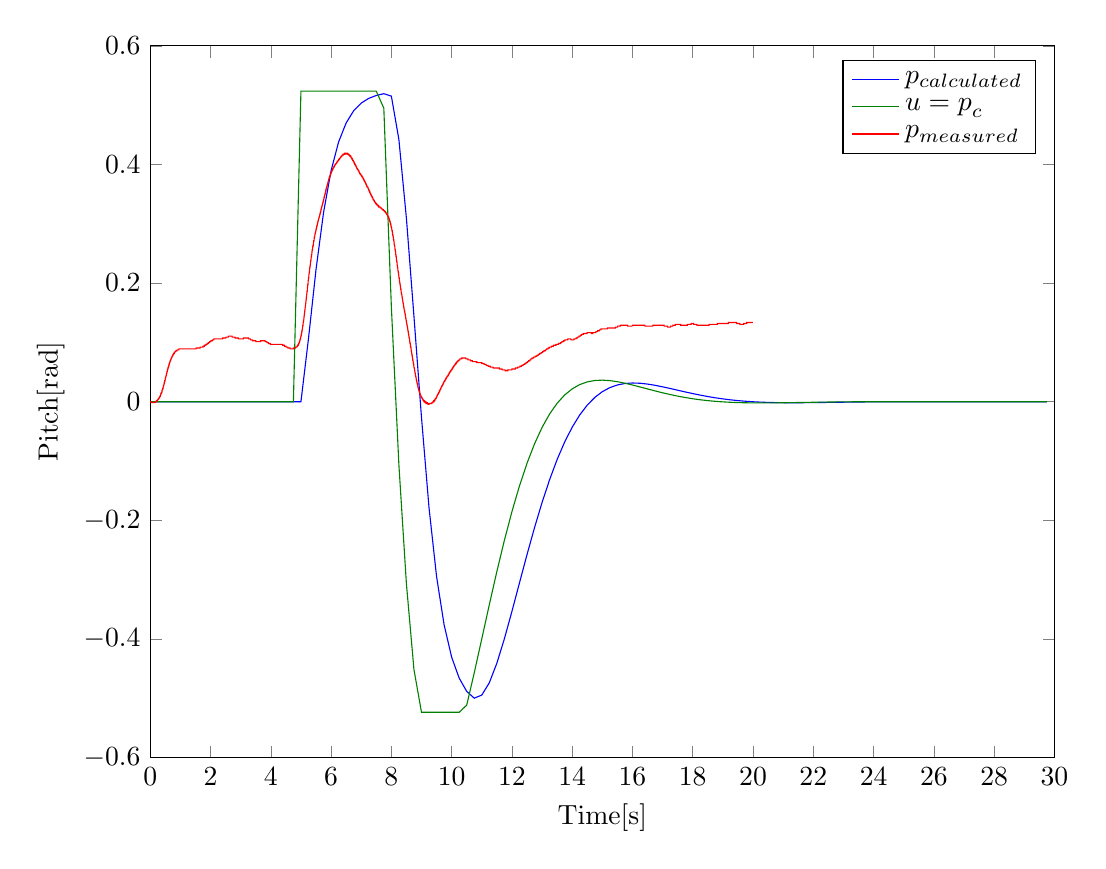
\begin{tikzpicture}

\begin{axis}[%
width=4.521in,
height=3.559in,
at={(0.758in,0.488in)},
scale only axis,
xmin=0,
xmax=30,
xlabel={Time[s]},
ymin=-0.6,
ymax=0.6,
ylabel={Pitch[rad]},
axis background/.style={fill=white},
legend style={legend cell align=left, align=left, draw=black}
]
\addplot [color=blue]
  table[row sep=crcr]{%
0	0\\
0.25	0\\
0.5	0\\
0.75	0\\
1	0\\
1.25	0\\
1.5	0\\
1.75	0\\
2	0\\
2.25	0\\
2.5	0\\
2.75	0\\
3	0\\
3.25	0\\
3.5	0\\
3.75	0\\
4	0\\
4.25	0\\
4.5	0\\
4.75	0\\
5	0\\
5.25	0.106028752058656\\
5.5	0.222660379323177\\
5.75	0.318881471816406\\
6	0.389443606311442\\
6.25	0.437955073776778\\
6.5	0.469972642303901\\
6.75	0.490517248775471\\
7	0.503431001414743\\
7.25	0.511421385860293\\
7.5	0.516304398577018\\
7.75	0.519258621270637\\
8	0.515203257617204\\
8.25	0.442077494057865\\
8.5	0.308917942206626\\
8.75	0.143857437412505\\
9	-0.0266421713474325\\
9.25	-0.178852015358114\\
9.5	-0.294706712119982\\
9.75	-0.376103400744807\\
10	-0.430593712461648\\
10.25	-0.465910557041165\\
10.5	-0.488275766784288\\
10.75	-0.499764190883541\\
11	-0.494606006688154\\
11.25	-0.473847629784875\\
11.5	-0.440912018084062\\
11.75	-0.399653357456757\\
12	-0.353578675828111\\
12.25	-0.305589905143908\\
12.5	-0.257949354898401\\
12.75	-0.212334914967486\\
13	-0.169924129646145\\
13.25	-0.131479200507158\\
13.5	-0.0974290818102873\\
13.75	-0.0679368059974756\\
14	-0.0429635308410175\\
14.25	-0.0223192342127769\\
14.5	-0.00570663885556016\\
14.75	0.00724201878417936\\
15	0.0169351049858723\\
15.25	0.0237983108610476\\
15.5	0.028255199621864\\
15.75	0.0307122623875607\\
16	0.0315508532381054\\
16.25	0.0311187961644862\\
16.5	0.029725886927415\\
16.75	0.0276432096833793\\
17	0.0251019885053482\\
17.25	0.0222957734120814\\
17.5	0.0193816640201188\\
17.75	0.0164843000616491\\
18	0.0136996386848572\\
18.25	0.0110954475341745\\
18.5	0.00871894022650019\\
18.75	0.0065986832260201\\
19	0.00474786933352292\\
19.25	0.00316789726194727\\
19.5	0.00185011308215904\\
19.75	0.000778241874597928\\
20	-6.67869857700027e-05\\
20.25	-0.000708334391687312\\
20.5	-0.00117133750514035\\
20.75	-0.0014797646315738\\
21	-0.00165871055146624\\
21.25	-0.00173215070440505\\
21.5	-0.00172140027657165\\
21.75	-0.00164528745713995\\
22	-0.00152183353077441\\
22.25	-0.00136650821059555\\
22.5	-0.00119259796958174\\
22.75	-0.001011086656585\\
23	-0.000832064472986232\\
23.25	-0.000663037040451166\\
23.5	-0.000510056885363023\\
23.75	-0.000377485451768905\\
24	-0.000268095912811798\\
24.25	-0.000182536382336601\\
24.5	-0.000119409133283147\\
24.75	-7.58389556319519e-05\\
25	0\\
25.25	0\\
25.5	0\\
25.75	0\\
26	0\\
26.25	0\\
26.5	0\\
26.75	0\\
27	0\\
27.25	0\\
27.5	0\\
27.75	0\\
28	0\\
28.25	0\\
28.5	0\\
28.75	0\\
29	0\\
29.25	0\\
29.5	0\\
29.75	0\\
};
\addlegendentry{$\text{p}_{\text{calculated}}$}

\addplot [color=black!50!green]
  table[row sep=crcr]{%
0	0\\
0.25	0\\
0.5	0\\
0.75	0\\
1	0\\
1.25	0\\
1.5	0\\
1.75	0\\
2	0\\
2.25	0\\
2.5	0\\
2.75	0\\
3	0\\
3.25	0\\
3.5	0\\
3.75	0\\
4	0\\
4.25	0\\
4.5	0\\
4.75	0\\
5	0.523598775598299\\
5.25	0.523598775598299\\
5.5	0.523598775598299\\
5.75	0.523598775598299\\
6	0.523598775598299\\
6.25	0.523598775598299\\
6.5	0.523598775598299\\
6.75	0.523598775598299\\
7	0.523598775598299\\
7.25	0.523598775598299\\
7.5	0.523598775598299\\
7.75	0.494819035995318\\
8	0.160146388213864\\
8.25	-0.106263288038621\\
8.5	-0.307278306480395\\
8.75	-0.451544073993497\\
9	-0.523598775598299\\
9.25	-0.523598775598299\\
9.5	-0.523598775598299\\
9.75	-0.523598775598299\\
10	-0.523598775598299\\
10.25	-0.523598775598299\\
10.5	-0.511598967534701\\
10.75	-0.457129956387681\\
11	-0.399800939111984\\
11.25	-0.342212060957365\\
11.5	-0.286365657156611\\
11.75	-0.23375737331411\\
12	-0.185424703030395\\
12.25	-0.142014857669656\\
12.5	-0.10385960931001\\
12.75	-0.0710390273514893\\
13	-0.0434270107361158\\
13.25	-0.0207605455327021\\
13.5	-0.00265320572629543\\
13.75	0.0113316469560184\\
14	0.021677856286943\\
14.25	0.0288792627115391\\
14.5	0.0334210033379285\\
14.75	0.0357660546640398\\
15	0.0363476842409992\\
15.25	0.0355551947305582\\
15.5	0.0337310214270478\\
15.75	0.0311830246785309\\
16	0.0281645282706534\\
16.25	0.0248856506222575\\
16.5	0.0215218266813817\\
16.75	0.0182051291317236\\
17	0.0150402814094847\\
17.25	0.0120971100725783\\
17.5	0.00942686961319992\\
17.75	0.00706104683026745\\
18	0.00499923826903931\\
18.25	0.00324982044976549\\
18.5	0.00179862644917375\\
18.75	0.000626159029220361\\
19	-0.000289665822503038\\
19.25	-0.000979473741196441\\
19.5	-0.00147453626685413\\
19.75	-0.00179354982950428\\
20	-0.0019725952606145\\
20.25	-0.00203640858014681\\
20.5	-0.00200278779953004\\
20.75	-0.00190271136809885\\
21	-0.0017540636979914\\
21.25	-0.00156935527676361\\
21.5	-0.00136159378268476\\
21.75	-0.00114933783497971\\
22	-0.000939213740881632\\
22.25	-0.000739721387584646\\
22.5	-0.000556037648149353\\
22.75	-0.00039817301995658\\
23	-0.00026478930263345\\
23.25	-0.000160077254049755\\
23.5	-8.39090499064568e-05\\
23.75	-3.5329005868231e-05\\
24	-8.98877730230801e-06\\
24.25	1.39196869899203e-06\\
24.5	1.45103863055569e-06\\
24.75	3.68703061246105e-07\\
25	0\\
25.25	0\\
25.5	0\\
25.75	0\\
26	0\\
26.25	0\\
26.5	0\\
26.75	0\\
27	0\\
27.25	0\\
27.5	0\\
27.75	0\\
28	0\\
28.25	0\\
28.5	0\\
28.75	0\\
29	0\\
29.25	0\\
29.5	0\\
29.75	0\\
};
\addlegendentry{$\text{u = p}_{\text{c}}$}

\addplot [color=red, forget plot]
  table[row sep=crcr]{%
0	0\\
0.002	0\\
0.004	0\\
0.006	0\\
0.008	0\\
0.01	0\\
0.012	0\\
0.014	0\\
0.016	0\\
0.018	0\\
0.02	0\\
0.022	0\\
0.024	0\\
0.026	0\\
0.028	0\\
0.03	0\\
0.032	0\\
0.034	0\\
0.036	0\\
0.038	0\\
0.04	0\\
0.042	0\\
0.044	0\\
0.046	0\\
0.048	-0.00153398078788564\\
0.05	-0.00153398078788564\\
0.052	-0.00153398078788564\\
0.054	-0.00153398078788564\\
0.056	-0.00153398078788564\\
0.058	-0.00153398078788564\\
0.06	-0.00153398078788564\\
0.062	-0.00153398078788564\\
0.064	-0.00153398078788564\\
0.066	-0.00153398078788564\\
0.068	-0.00153398078788564\\
0.07	-0.00153398078788564\\
0.072	-0.00153398078788564\\
0.074	-0.00153398078788564\\
0.076	-0.00153398078788564\\
0.078	-0.00153398078788564\\
0.08	-0.00153398078788564\\
0.082	-0.00153398078788564\\
0.084	-0.00153398078788564\\
0.086	-0.00153398078788564\\
0.088	-0.00153398078788564\\
0.09	-0.00153398078788564\\
0.092	-0.00153398078788564\\
0.094	-0.00153398078788564\\
0.096	-0.00153398078788564\\
0.098	-0.00153398078788564\\
0.1	-0.00153398078788564\\
0.102	-0.00153398078788564\\
0.104	-0.00153398078788564\\
0.106	-0.00153398078788564\\
0.108	-0.00153398078788564\\
0.11	-0.00153398078788564\\
0.112	-0.00153398078788564\\
0.114	-0.00153398078788564\\
0.116	-0.00153398078788564\\
0.118	-0.00153398078788564\\
0.12	-0.00153398078788564\\
0.122	-0.00153398078788564\\
0.124	-0.00153398078788564\\
0.126	-0.00153398078788564\\
0.128	-0.00153398078788564\\
0.13	-0.00153398078788564\\
0.132	-0.00153398078788564\\
0.134	-0.00153398078788564\\
0.136	-0.00153398078788564\\
0.138	-0.00153398078788564\\
0.14	-0.00153398078788564\\
0.142	-0.00153398078788564\\
0.144	-0.00153398078788564\\
0.146	-0.00153398078788564\\
0.148	-0.00153398078788564\\
0.15	-0.00153398078788564\\
0.152	-0.00153398078788564\\
0.154	-0.00153398078788564\\
0.156	-0.00153398078788564\\
0.158	-0.00153398078788564\\
0.16	-0.00153398078788564\\
0.162	-0.00153398078788564\\
0.164	-0.00153398078788564\\
0.166	0\\
0.168	0\\
0.17	0\\
0.172	0\\
0.174	0\\
0.176	0\\
0.178	0\\
0.18	0\\
0.182	0\\
0.184	0\\
0.186	0\\
0.188	0\\
0.19	0\\
0.192	0\\
0.194	0\\
0.196	0\\
0.198	0\\
0.2	0\\
0.202	0\\
0.204	0\\
0.206	0\\
0.208	0.00153398078788564\\
0.21	0.00153398078788564\\
0.212	0.00153398078788564\\
0.214	0.00153398078788564\\
0.216	0.00153398078788564\\
0.218	0.00153398078788564\\
0.22	0.00153398078788564\\
0.222	0.00153398078788564\\
0.224	0.00153398078788564\\
0.226	0.00153398078788564\\
0.228	0.00153398078788564\\
0.23	0.00153398078788564\\
0.232	0.00153398078788564\\
0.234	0.00153398078788564\\
0.236	0.00153398078788564\\
0.238	0.00153398078788564\\
0.24	0.00306796157577128\\
0.242	0.00306796157577128\\
0.244	0.00306796157577128\\
0.246	0.00306796157577128\\
0.248	0.00306796157577128\\
0.25	0.00306796157577128\\
0.252	0.00306796157577128\\
0.254	0.00306796157577128\\
0.256	0.00306796157577128\\
0.258	0.00306796157577128\\
0.26	0.00306796157577128\\
0.262	0.00306796157577128\\
0.264	0.00306796157577128\\
0.266	0.00460194236365692\\
0.268	0.00460194236365692\\
0.27	0.00460194236365692\\
0.272	0.00460194236365692\\
0.274	0.00460194236365692\\
0.276	0.00460194236365692\\
0.278	0.00460194236365692\\
0.28	0.00460194236365692\\
0.282	0.00613592315154256\\
0.284	0.00613592315154256\\
0.286	0.00613592315154256\\
0.288	0.00613592315154256\\
0.29	0.00613592315154256\\
0.292	0.00613592315154256\\
0.294	0.00613592315154256\\
0.296	0.00613592315154256\\
0.298	0.00613592315154256\\
0.3	0.00613592315154256\\
0.302	0.00613592315154256\\
0.304	0.00613592315154256\\
0.306	0.00766990393942821\\
0.308	0.00766990393942821\\
0.31	0.00766990393942821\\
0.312	0.00766990393942821\\
0.314	0.00766990393942821\\
0.316	0.00766990393942821\\
0.318	0.00920388472731385\\
0.32	0.00920388472731385\\
0.322	0.00920388472731385\\
0.324	0.00920388472731385\\
0.326	0.00920388472731385\\
0.328	0.00920388472731385\\
0.33	0.00920388472731385\\
0.332	0.00920388472731385\\
0.334	0.00920388472731385\\
0.336	0.00920388472731385\\
0.338	0.00920388472731385\\
0.34	0.0107378655151995\\
0.342	0.0107378655151995\\
0.344	0.0107378655151995\\
0.346	0.0107378655151995\\
0.348	0.0122718463030851\\
0.35	0.0122718463030851\\
0.352	0.0122718463030851\\
0.354	0.0122718463030851\\
0.356	0.0138058270909708\\
0.358	0.0138058270909708\\
0.36	0.0138058270909708\\
0.362	0.0138058270909708\\
0.364	0.0138058270909708\\
0.366	0.0138058270909708\\
0.368	0.0138058270909708\\
0.37	0.0153398078788564\\
0.372	0.0153398078788564\\
0.374	0.0153398078788564\\
0.376	0.0153398078788564\\
0.378	0.0153398078788564\\
0.38	0.0153398078788564\\
0.382	0.0153398078788564\\
0.384	0.0168737886667421\\
0.386	0.0184077694546277\\
0.388	0.0184077694546277\\
0.39	0.0168737886667421\\
0.392	0.0168737886667421\\
0.394	0.0184077694546277\\
0.396	0.0184077694546277\\
0.398	0.0199417502425133\\
0.4	0.0199417502425133\\
0.402	0.0199417502425133\\
0.404	0.0199417502425133\\
0.406	0.0199417502425133\\
0.408	0.0199417502425133\\
0.41	0.021475731030399\\
0.412	0.021475731030399\\
0.414	0.0230097118182846\\
0.416	0.021475731030399\\
0.418	0.021475731030399\\
0.42	0.021475731030399\\
0.422	0.021475731030399\\
0.424	0.0230097118182846\\
0.426	0.0245436926061703\\
0.428	0.0245436926061703\\
0.43	0.0245436926061703\\
0.432	0.0245436926061703\\
0.434	0.0245436926061703\\
0.436	0.0260776733940559\\
0.438	0.0260776733940559\\
0.44	0.0276116541819415\\
0.442	0.0276116541819415\\
0.444	0.0276116541819415\\
0.446	0.0276116541819415\\
0.448	0.0276116541819415\\
0.45	0.0276116541819415\\
0.452	0.0291456349698272\\
0.454	0.0291456349698272\\
0.456	0.0291456349698272\\
0.458	0.0291456349698272\\
0.46	0.0291456349698272\\
0.462	0.0306796157577128\\
0.464	0.0306796157577128\\
0.466	0.0322135965455985\\
0.468	0.0322135965455985\\
0.47	0.0322135965455985\\
0.472	0.0322135965455985\\
0.474	0.0322135965455985\\
0.476	0.0337475773334841\\
0.478	0.0337475773334841\\
0.48	0.0337475773334841\\
0.482	0.0352815581213697\\
0.484	0.0352815581213697\\
0.486	0.0352815581213697\\
0.488	0.0352815581213697\\
0.49	0.0352815581213697\\
0.492	0.0368155389092554\\
0.494	0.0368155389092554\\
0.496	0.038349519697141\\
0.498	0.038349519697141\\
0.5	0.038349519697141\\
0.502	0.038349519697141\\
0.504	0.038349519697141\\
0.506	0.0398835004850267\\
0.508	0.0398835004850267\\
0.51	0.0414174812729123\\
0.512	0.0414174812729123\\
0.514	0.0414174812729123\\
0.516	0.0414174812729123\\
0.518	0.0414174812729123\\
0.52	0.0414174812729123\\
0.522	0.042951462060798\\
0.524	0.042951462060798\\
0.526	0.0444854428486836\\
0.528	0.0444854428486836\\
0.53	0.0444854428486836\\
0.532	0.0444854428486836\\
0.534	0.0444854428486836\\
0.536	0.0460194236365692\\
0.538	0.0460194236365692\\
0.54	0.0475534044244549\\
0.542	0.0475534044244549\\
0.544	0.0475534044244549\\
0.546	0.0475534044244549\\
0.548	0.0475534044244549\\
0.55	0.0490873852123405\\
0.552	0.0490873852123405\\
0.554	0.0490873852123405\\
0.556	0.0506213660002262\\
0.558	0.0506213660002262\\
0.56	0.0506213660002262\\
0.562	0.0506213660002262\\
0.564	0.0506213660002262\\
0.566	0.0521553467881118\\
0.568	0.0521553467881118\\
0.57	0.0521553467881118\\
0.572	0.0536893275759974\\
0.574	0.0536893275759974\\
0.576	0.0536893275759974\\
0.578	0.0536893275759974\\
0.58	0.0536893275759974\\
0.582	0.0552233083638831\\
0.584	0.0552233083638831\\
0.586	0.0552233083638831\\
0.588	0.0552233083638831\\
0.59	0.0567572891517687\\
0.592	0.0567572891517687\\
0.594	0.0567572891517687\\
0.596	0.0567572891517687\\
0.598	0.0582912699396544\\
0.6	0.0582912699396544\\
0.602	0.0582912699396544\\
0.604	0.0582912699396544\\
0.606	0.0582912699396544\\
0.608	0.05982525072754\\
0.61	0.05982525072754\\
0.612	0.05982525072754\\
0.614	0.05982525072754\\
0.616	0.0613592315154256\\
0.618	0.0613592315154256\\
0.62	0.0613592315154256\\
0.622	0.0613592315154256\\
0.624	0.0628932123033113\\
0.626	0.0628932123033113\\
0.628	0.0628932123033113\\
0.63	0.0628932123033113\\
0.632	0.0644271930911969\\
0.634	0.0644271930911969\\
0.636	0.0644271930911969\\
0.638	0.0644271930911969\\
0.64	0.0644271930911969\\
0.642	0.0644271930911969\\
0.644	0.0659611738790826\\
0.646	0.0659611738790826\\
0.648	0.0659611738790826\\
0.65	0.0659611738790826\\
0.652	0.0659611738790826\\
0.654	0.0674951546669682\\
0.656	0.0674951546669682\\
0.658	0.0674951546669682\\
0.66	0.0674951546669682\\
0.662	0.0674951546669682\\
0.664	0.0690291354548539\\
0.666	0.0690291354548539\\
0.668	0.0690291354548539\\
0.67	0.0690291354548539\\
0.672	0.0690291354548539\\
0.674	0.0705631162427395\\
0.676	0.0705631162427395\\
0.678	0.0705631162427395\\
0.68	0.0705631162427395\\
0.682	0.0705631162427395\\
0.684	0.0705631162427395\\
0.686	0.0705631162427395\\
0.688	0.0720970970306251\\
0.69	0.0720970970306251\\
0.692	0.0720970970306251\\
0.694	0.0720970970306251\\
0.696	0.0720970970306251\\
0.698	0.0720970970306251\\
0.7	0.0736310778185108\\
0.702	0.0736310778185108\\
0.704	0.0736310778185108\\
0.706	0.0736310778185108\\
0.708	0.0736310778185108\\
0.71	0.0736310778185108\\
0.712	0.0751650586063964\\
0.714	0.0751650586063964\\
0.716	0.0751650586063964\\
0.718	0.0751650586063964\\
0.72	0.0751650586063964\\
0.722	0.0751650586063964\\
0.724	0.0751650586063964\\
0.726	0.0766990393942821\\
0.728	0.0766990393942821\\
0.73	0.0766990393942821\\
0.732	0.0766990393942821\\
0.734	0.0766990393942821\\
0.736	0.0766990393942821\\
0.738	0.0766990393942821\\
0.74	0.0766990393942821\\
0.742	0.0782330201821677\\
0.744	0.0782330201821677\\
0.746	0.0782330201821677\\
0.748	0.0782330201821677\\
0.75	0.0782330201821677\\
0.752	0.0782330201821677\\
0.754	0.0782330201821677\\
0.756	0.0797670009700533\\
0.758	0.0797670009700533\\
0.76	0.0797670009700533\\
0.762	0.0797670009700533\\
0.764	0.0797670009700533\\
0.766	0.0797670009700533\\
0.768	0.0797670009700533\\
0.77	0.0797670009700533\\
0.772	0.0797670009700533\\
0.774	0.0797670009700533\\
0.776	0.081300981757939\\
0.778	0.081300981757939\\
0.78	0.081300981757939\\
0.782	0.081300981757939\\
0.784	0.081300981757939\\
0.786	0.081300981757939\\
0.788	0.081300981757939\\
0.79	0.081300981757939\\
0.792	0.081300981757939\\
0.794	0.081300981757939\\
0.796	0.081300981757939\\
0.798	0.0828349625458246\\
0.8	0.0828349625458246\\
0.802	0.0828349625458246\\
0.804	0.0828349625458246\\
0.806	0.0828349625458246\\
0.808	0.0828349625458246\\
0.81	0.0828349625458246\\
0.812	0.0828349625458246\\
0.814	0.0828349625458246\\
0.816	0.0828349625458246\\
0.818	0.0843689433337103\\
0.82	0.0843689433337103\\
0.822	0.0843689433337103\\
0.824	0.0843689433337103\\
0.826	0.0843689433337103\\
0.828	0.0843689433337103\\
0.83	0.0843689433337103\\
0.832	0.0843689433337103\\
0.834	0.0843689433337103\\
0.836	0.0843689433337103\\
0.838	0.0843689433337103\\
0.84	0.0843689433337103\\
0.842	0.0843689433337103\\
0.844	0.0843689433337103\\
0.846	0.0843689433337103\\
0.848	0.0843689433337103\\
0.85	0.0843689433337103\\
0.852	0.0859029241215959\\
0.854	0.0859029241215959\\
0.856	0.0859029241215959\\
0.858	0.0859029241215959\\
0.86	0.0859029241215959\\
0.862	0.0859029241215959\\
0.864	0.0859029241215959\\
0.866	0.0859029241215959\\
0.868	0.0859029241215959\\
0.87	0.0859029241215959\\
0.872	0.0859029241215959\\
0.874	0.0859029241215959\\
0.876	0.0859029241215959\\
0.878	0.0859029241215959\\
0.88	0.0859029241215959\\
0.882	0.0859029241215959\\
0.884	0.0859029241215959\\
0.886	0.0859029241215959\\
0.888	0.0859029241215959\\
0.89	0.0859029241215959\\
0.892	0.0874369049094816\\
0.894	0.0874369049094816\\
0.896	0.0874369049094816\\
0.898	0.0874369049094816\\
0.9	0.0874369049094816\\
0.902	0.0874369049094816\\
0.904	0.0874369049094816\\
0.906	0.0874369049094816\\
0.908	0.0874369049094816\\
0.91	0.0874369049094816\\
0.912	0.0874369049094816\\
0.914	0.0874369049094816\\
0.916	0.0874369049094816\\
0.918	0.0874369049094816\\
0.92	0.0874369049094816\\
0.922	0.0874369049094816\\
0.924	0.0874369049094816\\
0.926	0.0874369049094816\\
0.928	0.0874369049094816\\
0.93	0.0874369049094816\\
0.932	0.0874369049094816\\
0.934	0.0874369049094816\\
0.936	0.0874369049094816\\
0.938	0.0874369049094816\\
0.94	0.0874369049094816\\
0.942	0.0874369049094816\\
0.944	0.0874369049094816\\
0.946	0.0874369049094816\\
0.948	0.0874369049094816\\
0.95	0.0874369049094816\\
0.952	0.0889708856973672\\
0.954	0.0889708856973672\\
0.956	0.0889708856973672\\
0.958	0.0889708856973672\\
0.96	0.0889708856973672\\
0.962	0.0889708856973672\\
0.964	0.0889708856973672\\
0.966	0.0889708856973672\\
0.968	0.0889708856973672\\
0.97	0.0889708856973672\\
0.972	0.0889708856973672\\
0.974	0.0889708856973672\\
0.976	0.0889708856973672\\
0.978	0.0889708856973672\\
0.98	0.0889708856973672\\
0.982	0.0889708856973672\\
0.984	0.0889708856973672\\
0.986	0.0889708856973672\\
0.988	0.0889708856973672\\
0.99	0.0889708856973672\\
0.992	0.0889708856973672\\
0.994	0.0889708856973672\\
0.996	0.0889708856973672\\
0.998	0.0889708856973672\\
1	0.0889708856973672\\
1.002	0.0889708856973672\\
1.004	0.0889708856973672\\
1.006	0.0889708856973672\\
1.008	0.0889708856973672\\
1.01	0.0889708856973672\\
1.012	0.0889708856973672\\
1.014	0.0889708856973672\\
1.016	0.0889708856973672\\
1.018	0.0889708856973672\\
1.02	0.0889708856973672\\
1.022	0.0889708856973672\\
1.024	0.0889708856973672\\
1.026	0.0889708856973672\\
1.028	0.0889708856973672\\
1.03	0.0889708856973672\\
1.032	0.0889708856973672\\
1.034	0.0889708856973672\\
1.036	0.0889708856973672\\
1.038	0.0889708856973672\\
1.04	0.0889708856973672\\
1.042	0.0889708856973672\\
1.044	0.0889708856973672\\
1.046	0.0889708856973672\\
1.048	0.0889708856973672\\
1.05	0.0889708856973672\\
1.052	0.0889708856973672\\
1.054	0.0889708856973672\\
1.056	0.0889708856973672\\
1.058	0.0889708856973672\\
1.06	0.0889708856973672\\
1.062	0.0889708856973672\\
1.064	0.0889708856973672\\
1.066	0.0889708856973672\\
1.068	0.0889708856973672\\
1.07	0.0889708856973672\\
1.072	0.0889708856973672\\
1.074	0.0889708856973672\\
1.076	0.0889708856973672\\
1.078	0.0889708856973672\\
1.08	0.0889708856973672\\
1.082	0.0889708856973672\\
1.084	0.0889708856973672\\
1.086	0.0889708856973672\\
1.088	0.0889708856973672\\
1.09	0.0889708856973672\\
1.092	0.0889708856973672\\
1.094	0.0889708856973672\\
1.096	0.0889708856973672\\
1.098	0.0889708856973672\\
1.1	0.0889708856973672\\
1.102	0.0889708856973672\\
1.104	0.0889708856973672\\
1.106	0.0889708856973672\\
1.108	0.0889708856973672\\
1.11	0.0889708856973672\\
1.112	0.0889708856973672\\
1.114	0.0889708856973672\\
1.116	0.0889708856973672\\
1.118	0.0889708856973672\\
1.12	0.0889708856973672\\
1.122	0.0889708856973672\\
1.124	0.0889708856973672\\
1.126	0.0889708856973672\\
1.128	0.0889708856973672\\
1.13	0.0889708856973672\\
1.132	0.0889708856973672\\
1.134	0.0889708856973672\\
1.136	0.0889708856973672\\
1.138	0.0889708856973672\\
1.14	0.0889708856973672\\
1.142	0.0889708856973672\\
1.144	0.0889708856973672\\
1.146	0.0889708856973672\\
1.148	0.0889708856973672\\
1.15	0.0889708856973672\\
1.152	0.0889708856973672\\
1.154	0.0889708856973672\\
1.156	0.0889708856973672\\
1.158	0.0889708856973672\\
1.16	0.0889708856973672\\
1.162	0.0889708856973672\\
1.164	0.0889708856973672\\
1.166	0.0889708856973672\\
1.168	0.0889708856973672\\
1.17	0.0889708856973672\\
1.172	0.0889708856973672\\
1.174	0.0889708856973672\\
1.176	0.0889708856973672\\
1.178	0.0889708856973672\\
1.18	0.0889708856973672\\
1.182	0.0889708856973672\\
1.184	0.0889708856973672\\
1.186	0.0889708856973672\\
1.188	0.0889708856973672\\
1.19	0.0889708856973672\\
1.192	0.0889708856973672\\
1.194	0.0889708856973672\\
1.196	0.0889708856973672\\
1.198	0.0889708856973672\\
1.2	0.0889708856973672\\
1.202	0.0889708856973672\\
1.204	0.0889708856973672\\
1.206	0.0889708856973672\\
1.208	0.0889708856973672\\
1.21	0.0889708856973672\\
1.212	0.0889708856973672\\
1.214	0.0889708856973672\\
1.216	0.0889708856973672\\
1.218	0.0889708856973672\\
1.22	0.0889708856973672\\
1.222	0.0889708856973672\\
1.224	0.0889708856973672\\
1.226	0.0889708856973672\\
1.228	0.0889708856973672\\
1.23	0.0889708856973672\\
1.232	0.0889708856973672\\
1.234	0.0889708856973672\\
1.236	0.0889708856973672\\
1.238	0.0889708856973672\\
1.24	0.0889708856973672\\
1.242	0.0889708856973672\\
1.244	0.0889708856973672\\
1.246	0.0889708856973672\\
1.248	0.0889708856973672\\
1.25	0.0889708856973672\\
1.252	0.0889708856973672\\
1.254	0.0889708856973672\\
1.256	0.0889708856973672\\
1.258	0.0889708856973672\\
1.26	0.0889708856973672\\
1.262	0.0889708856973672\\
1.264	0.0889708856973672\\
1.266	0.0889708856973672\\
1.268	0.0889708856973672\\
1.27	0.0889708856973672\\
1.272	0.0889708856973672\\
1.274	0.0889708856973672\\
1.276	0.0889708856973672\\
1.278	0.0889708856973672\\
1.28	0.0889708856973672\\
1.282	0.0889708856973672\\
1.284	0.0889708856973672\\
1.286	0.0889708856973672\\
1.288	0.0889708856973672\\
1.29	0.0889708856973672\\
1.292	0.0889708856973672\\
1.294	0.0889708856973672\\
1.296	0.0889708856973672\\
1.298	0.0889708856973672\\
1.3	0.0889708856973672\\
1.302	0.0889708856973672\\
1.304	0.0889708856973672\\
1.306	0.0889708856973672\\
1.308	0.0889708856973672\\
1.31	0.0889708856973672\\
1.312	0.0889708856973672\\
1.314	0.0889708856973672\\
1.316	0.0889708856973672\\
1.318	0.0889708856973672\\
1.32	0.0889708856973672\\
1.322	0.0889708856973672\\
1.324	0.0889708856973672\\
1.326	0.0889708856973672\\
1.328	0.0889708856973672\\
1.33	0.0889708856973672\\
1.332	0.0889708856973672\\
1.334	0.0889708856973672\\
1.336	0.0889708856973672\\
1.338	0.0889708856973672\\
1.34	0.0889708856973672\\
1.342	0.0889708856973672\\
1.344	0.0889708856973672\\
1.346	0.0889708856973672\\
1.348	0.0889708856973672\\
1.35	0.0889708856973672\\
1.352	0.0889708856973672\\
1.354	0.0889708856973672\\
1.356	0.0889708856973672\\
1.358	0.0889708856973672\\
1.36	0.0889708856973672\\
1.362	0.0889708856973672\\
1.364	0.0889708856973672\\
1.366	0.0889708856973672\\
1.368	0.0889708856973672\\
1.37	0.0889708856973672\\
1.372	0.0889708856973672\\
1.374	0.0889708856973672\\
1.376	0.0889708856973672\\
1.378	0.0889708856973672\\
1.38	0.0889708856973672\\
1.382	0.0889708856973672\\
1.384	0.0889708856973672\\
1.386	0.0889708856973672\\
1.388	0.0889708856973672\\
1.39	0.0889708856973672\\
1.392	0.0889708856973672\\
1.394	0.0889708856973672\\
1.396	0.0889708856973672\\
1.398	0.0889708856973672\\
1.4	0.0889708856973672\\
1.402	0.0889708856973672\\
1.404	0.0889708856973672\\
1.406	0.0889708856973672\\
1.408	0.0889708856973672\\
1.41	0.0889708856973672\\
1.412	0.0889708856973672\\
1.414	0.0889708856973672\\
1.416	0.0889708856973672\\
1.418	0.0889708856973672\\
1.42	0.0889708856973672\\
1.422	0.0889708856973672\\
1.424	0.0889708856973672\\
1.426	0.0889708856973672\\
1.428	0.0889708856973672\\
1.43	0.0889708856973672\\
1.432	0.0889708856973672\\
1.434	0.0889708856973672\\
1.436	0.0889708856973672\\
1.438	0.0889708856973672\\
1.44	0.0889708856973672\\
1.442	0.0889708856973672\\
1.444	0.0889708856973672\\
1.446	0.0889708856973672\\
1.448	0.0889708856973672\\
1.45	0.0889708856973672\\
1.452	0.0889708856973672\\
1.454	0.0889708856973672\\
1.456	0.0889708856973672\\
1.458	0.0889708856973672\\
1.46	0.0889708856973672\\
1.462	0.0889708856973672\\
1.464	0.0889708856973672\\
1.466	0.0889708856973672\\
1.468	0.0889708856973672\\
1.47	0.0889708856973672\\
1.472	0.0889708856973672\\
1.474	0.0889708856973672\\
1.476	0.0889708856973672\\
1.478	0.0889708856973672\\
1.48	0.0889708856973672\\
1.482	0.0889708856973672\\
1.484	0.0889708856973672\\
1.486	0.0889708856973672\\
1.488	0.0889708856973672\\
1.49	0.0889708856973672\\
1.492	0.0889708856973672\\
1.494	0.0889708856973672\\
1.496	0.0889708856973672\\
1.498	0.0889708856973672\\
1.5	0.0889708856973672\\
1.502	0.0889708856973672\\
1.504	0.0889708856973672\\
1.506	0.0889708856973672\\
1.508	0.0889708856973672\\
1.51	0.0889708856973672\\
1.512	0.0889708856973672\\
1.514	0.0889708856973672\\
1.516	0.0889708856973672\\
1.518	0.0889708856973672\\
1.52	0.0889708856973672\\
1.522	0.0889708856973672\\
1.524	0.0905048664852528\\
1.526	0.0905048664852528\\
1.528	0.0905048664852528\\
1.53	0.0905048664852528\\
1.532	0.0905048664852528\\
1.534	0.0905048664852528\\
1.536	0.0905048664852528\\
1.538	0.0905048664852528\\
1.54	0.0905048664852528\\
1.542	0.0905048664852528\\
1.544	0.0905048664852528\\
1.546	0.0905048664852528\\
1.548	0.0905048664852528\\
1.55	0.0905048664852528\\
1.552	0.0905048664852528\\
1.554	0.0905048664852528\\
1.556	0.0905048664852528\\
1.558	0.0905048664852528\\
1.56	0.0905048664852528\\
1.562	0.0905048664852528\\
1.564	0.0905048664852528\\
1.566	0.0905048664852528\\
1.568	0.0905048664852528\\
1.57	0.0905048664852528\\
1.572	0.0905048664852528\\
1.574	0.0905048664852528\\
1.576	0.0905048664852528\\
1.578	0.0905048664852528\\
1.58	0.0905048664852528\\
1.582	0.0905048664852528\\
1.584	0.0905048664852528\\
1.586	0.0905048664852528\\
1.588	0.0905048664852528\\
1.59	0.0905048664852528\\
1.592	0.0905048664852528\\
1.594	0.0905048664852528\\
1.596	0.0905048664852528\\
1.598	0.0905048664852528\\
1.6	0.0905048664852528\\
1.602	0.0905048664852528\\
1.604	0.0905048664852528\\
1.606	0.0905048664852528\\
1.608	0.0905048664852528\\
1.61	0.0905048664852528\\
1.612	0.0905048664852528\\
1.614	0.0905048664852528\\
1.616	0.0905048664852528\\
1.618	0.0905048664852528\\
1.62	0.0905048664852528\\
1.622	0.0905048664852528\\
1.624	0.0905048664852528\\
1.626	0.0905048664852528\\
1.628	0.0905048664852528\\
1.63	0.0905048664852528\\
1.632	0.0905048664852528\\
1.634	0.0905048664852528\\
1.636	0.0905048664852528\\
1.638	0.0905048664852528\\
1.64	0.0905048664852528\\
1.642	0.0905048664852528\\
1.644	0.0905048664852528\\
1.646	0.0905048664852528\\
1.648	0.0905048664852528\\
1.65	0.0905048664852528\\
1.652	0.0905048664852528\\
1.654	0.0920388472731385\\
1.656	0.0920388472731385\\
1.658	0.0920388472731385\\
1.66	0.0920388472731385\\
1.662	0.0920388472731385\\
1.664	0.0920388472731385\\
1.666	0.0920388472731385\\
1.668	0.0920388472731385\\
1.67	0.0920388472731385\\
1.672	0.0920388472731385\\
1.674	0.0920388472731385\\
1.676	0.0920388472731385\\
1.678	0.0920388472731385\\
1.68	0.0920388472731385\\
1.682	0.0920388472731385\\
1.684	0.0920388472731385\\
1.686	0.0920388472731385\\
1.688	0.0920388472731385\\
1.69	0.0920388472731385\\
1.692	0.0920388472731385\\
1.694	0.0920388472731385\\
1.696	0.0920388472731385\\
1.698	0.0920388472731385\\
1.7	0.0920388472731385\\
1.702	0.0920388472731385\\
1.704	0.0920388472731385\\
1.706	0.0920388472731385\\
1.708	0.0920388472731385\\
1.71	0.0920388472731385\\
1.712	0.0920388472731385\\
1.714	0.0920388472731385\\
1.716	0.0920388472731385\\
1.718	0.0920388472731385\\
1.72	0.0920388472731385\\
1.722	0.0920388472731385\\
1.724	0.0920388472731385\\
1.726	0.0920388472731385\\
1.728	0.0920388472731385\\
1.73	0.0920388472731385\\
1.732	0.0920388472731385\\
1.734	0.0920388472731385\\
1.736	0.0920388472731385\\
1.738	0.0920388472731385\\
1.74	0.0920388472731385\\
1.742	0.0920388472731385\\
1.744	0.0920388472731385\\
1.746	0.0920388472731385\\
1.748	0.0920388472731385\\
1.75	0.0920388472731385\\
1.752	0.0935728280610241\\
1.754	0.0935728280610241\\
1.756	0.0935728280610241\\
1.758	0.0935728280610241\\
1.76	0.0935728280610241\\
1.762	0.0935728280610241\\
1.764	0.0935728280610241\\
1.766	0.0935728280610241\\
1.768	0.0935728280610241\\
1.77	0.0935728280610241\\
1.772	0.0935728280610241\\
1.774	0.0935728280610241\\
1.776	0.0935728280610241\\
1.778	0.0935728280610241\\
1.78	0.0935728280610241\\
1.782	0.0935728280610241\\
1.784	0.0935728280610241\\
1.786	0.0935728280610241\\
1.788	0.0935728280610241\\
1.79	0.0935728280610241\\
1.792	0.0935728280610241\\
1.794	0.0951068088489097\\
1.796	0.0951068088489097\\
1.798	0.0951068088489097\\
1.8	0.0951068088489097\\
1.802	0.0951068088489097\\
1.804	0.0951068088489097\\
1.806	0.0951068088489097\\
1.808	0.0951068088489097\\
1.81	0.0951068088489097\\
1.812	0.0951068088489097\\
1.814	0.0951068088489097\\
1.816	0.0951068088489097\\
1.818	0.0951068088489097\\
1.82	0.0951068088489097\\
1.822	0.0951068088489097\\
1.824	0.0951068088489097\\
1.826	0.0951068088489097\\
1.828	0.0951068088489097\\
1.83	0.0951068088489097\\
1.832	0.0951068088489097\\
1.834	0.0951068088489097\\
1.836	0.0951068088489097\\
1.838	0.0951068088489097\\
1.84	0.0951068088489097\\
1.842	0.0951068088489097\\
1.844	0.0951068088489097\\
1.846	0.0951068088489097\\
1.848	0.0951068088489097\\
1.85	0.0966407896367954\\
1.852	0.0966407896367954\\
1.854	0.0966407896367954\\
1.856	0.0966407896367954\\
1.858	0.0966407896367954\\
1.86	0.0966407896367954\\
1.862	0.0966407896367954\\
1.864	0.0966407896367954\\
1.866	0.0966407896367954\\
1.868	0.0966407896367954\\
1.87	0.0966407896367954\\
1.872	0.0966407896367954\\
1.874	0.0966407896367954\\
1.876	0.0966407896367954\\
1.878	0.0966407896367954\\
1.88	0.0966407896367954\\
1.882	0.0966407896367954\\
1.884	0.0966407896367954\\
1.886	0.0966407896367954\\
1.888	0.0966407896367954\\
1.89	0.098174770424681\\
1.892	0.098174770424681\\
1.894	0.098174770424681\\
1.896	0.098174770424681\\
1.898	0.098174770424681\\
1.9	0.098174770424681\\
1.902	0.098174770424681\\
1.904	0.098174770424681\\
1.906	0.098174770424681\\
1.908	0.098174770424681\\
1.91	0.098174770424681\\
1.912	0.098174770424681\\
1.914	0.098174770424681\\
1.916	0.098174770424681\\
1.918	0.098174770424681\\
1.92	0.098174770424681\\
1.922	0.098174770424681\\
1.924	0.098174770424681\\
1.926	0.098174770424681\\
1.928	0.098174770424681\\
1.93	0.098174770424681\\
1.932	0.0997087512125667\\
1.934	0.0997087512125667\\
1.936	0.0997087512125667\\
1.938	0.0997087512125667\\
1.94	0.0997087512125667\\
1.942	0.0997087512125667\\
1.944	0.0997087512125667\\
1.946	0.0997087512125667\\
1.948	0.0997087512125667\\
1.95	0.0997087512125667\\
1.952	0.0997087512125667\\
1.954	0.0997087512125667\\
1.956	0.0997087512125667\\
1.958	0.0997087512125667\\
1.96	0.0997087512125667\\
1.962	0.0997087512125667\\
1.964	0.0997087512125667\\
1.966	0.0997087512125667\\
1.968	0.0997087512125667\\
1.97	0.0997087512125667\\
1.972	0.101242732000452\\
1.974	0.101242732000452\\
1.976	0.101242732000452\\
1.978	0.101242732000452\\
1.98	0.101242732000452\\
1.982	0.101242732000452\\
1.984	0.101242732000452\\
1.986	0.101242732000452\\
1.988	0.101242732000452\\
1.99	0.101242732000452\\
1.992	0.101242732000452\\
1.994	0.101242732000452\\
1.996	0.101242732000452\\
1.998	0.101242732000452\\
2	0.101242732000452\\
2.002	0.101242732000452\\
2.004	0.101242732000452\\
2.006	0.101242732000452\\
2.008	0.101242732000452\\
2.01	0.101242732000452\\
2.012	0.101242732000452\\
2.014	0.102776712788338\\
2.016	0.102776712788338\\
2.018	0.102776712788338\\
2.02	0.102776712788338\\
2.022	0.102776712788338\\
2.024	0.102776712788338\\
2.026	0.102776712788338\\
2.028	0.102776712788338\\
2.03	0.102776712788338\\
2.032	0.102776712788338\\
2.034	0.102776712788338\\
2.036	0.102776712788338\\
2.038	0.102776712788338\\
2.04	0.102776712788338\\
2.042	0.102776712788338\\
2.044	0.102776712788338\\
2.046	0.102776712788338\\
2.048	0.102776712788338\\
2.05	0.102776712788338\\
2.052	0.102776712788338\\
2.054	0.102776712788338\\
2.056	0.102776712788338\\
2.058	0.102776712788338\\
2.06	0.102776712788338\\
2.062	0.102776712788338\\
2.064	0.102776712788338\\
2.066	0.104310693576224\\
2.068	0.104310693576224\\
2.07	0.104310693576224\\
2.072	0.104310693576224\\
2.074	0.104310693576224\\
2.076	0.104310693576224\\
2.078	0.104310693576224\\
2.08	0.104310693576224\\
2.082	0.104310693576224\\
2.084	0.104310693576224\\
2.086	0.104310693576224\\
2.088	0.104310693576224\\
2.09	0.104310693576224\\
2.092	0.104310693576224\\
2.094	0.104310693576224\\
2.096	0.104310693576224\\
2.098	0.104310693576224\\
2.1	0.104310693576224\\
2.102	0.104310693576224\\
2.104	0.104310693576224\\
2.106	0.104310693576224\\
2.108	0.104310693576224\\
2.11	0.104310693576224\\
2.112	0.105844674364109\\
2.114	0.105844674364109\\
2.116	0.105844674364109\\
2.118	0.105844674364109\\
2.12	0.105844674364109\\
2.122	0.105844674364109\\
2.124	0.105844674364109\\
2.126	0.105844674364109\\
2.128	0.105844674364109\\
2.13	0.105844674364109\\
2.132	0.105844674364109\\
2.134	0.105844674364109\\
2.136	0.105844674364109\\
2.138	0.105844674364109\\
2.14	0.105844674364109\\
2.142	0.105844674364109\\
2.144	0.105844674364109\\
2.146	0.105844674364109\\
2.148	0.105844674364109\\
2.15	0.105844674364109\\
2.152	0.105844674364109\\
2.154	0.105844674364109\\
2.156	0.105844674364109\\
2.158	0.105844674364109\\
2.16	0.105844674364109\\
2.162	0.105844674364109\\
2.164	0.105844674364109\\
2.166	0.105844674364109\\
2.168	0.105844674364109\\
2.17	0.105844674364109\\
2.172	0.105844674364109\\
2.174	0.105844674364109\\
2.176	0.105844674364109\\
2.178	0.105844674364109\\
2.18	0.105844674364109\\
2.182	0.105844674364109\\
2.184	0.105844674364109\\
2.186	0.105844674364109\\
2.188	0.105844674364109\\
2.19	0.105844674364109\\
2.192	0.105844674364109\\
2.194	0.105844674364109\\
2.196	0.105844674364109\\
2.198	0.105844674364109\\
2.2	0.105844674364109\\
2.202	0.105844674364109\\
2.204	0.105844674364109\\
2.206	0.105844674364109\\
2.208	0.105844674364109\\
2.21	0.105844674364109\\
2.212	0.105844674364109\\
2.214	0.105844674364109\\
2.216	0.105844674364109\\
2.218	0.105844674364109\\
2.22	0.105844674364109\\
2.222	0.105844674364109\\
2.224	0.105844674364109\\
2.226	0.105844674364109\\
2.228	0.105844674364109\\
2.23	0.105844674364109\\
2.232	0.105844674364109\\
2.234	0.105844674364109\\
2.236	0.105844674364109\\
2.238	0.105844674364109\\
2.24	0.105844674364109\\
2.242	0.105844674364109\\
2.244	0.105844674364109\\
2.246	0.105844674364109\\
2.248	0.105844674364109\\
2.25	0.105844674364109\\
2.252	0.105844674364109\\
2.254	0.105844674364109\\
2.256	0.105844674364109\\
2.258	0.105844674364109\\
2.26	0.105844674364109\\
2.262	0.105844674364109\\
2.264	0.105844674364109\\
2.266	0.105844674364109\\
2.268	0.105844674364109\\
2.27	0.105844674364109\\
2.272	0.105844674364109\\
2.274	0.105844674364109\\
2.276	0.105844674364109\\
2.278	0.105844674364109\\
2.28	0.105844674364109\\
2.282	0.105844674364109\\
2.284	0.105844674364109\\
2.286	0.105844674364109\\
2.288	0.105844674364109\\
2.29	0.105844674364109\\
2.292	0.105844674364109\\
2.294	0.105844674364109\\
2.296	0.105844674364109\\
2.298	0.105844674364109\\
2.3	0.105844674364109\\
2.302	0.105844674364109\\
2.304	0.105844674364109\\
2.306	0.105844674364109\\
2.308	0.105844674364109\\
2.31	0.105844674364109\\
2.312	0.105844674364109\\
2.314	0.105844674364109\\
2.316	0.105844674364109\\
2.318	0.105844674364109\\
2.32	0.105844674364109\\
2.322	0.105844674364109\\
2.324	0.105844674364109\\
2.326	0.105844674364109\\
2.328	0.105844674364109\\
2.33	0.105844674364109\\
2.332	0.105844674364109\\
2.334	0.105844674364109\\
2.336	0.105844674364109\\
2.338	0.105844674364109\\
2.34	0.105844674364109\\
2.342	0.105844674364109\\
2.344	0.105844674364109\\
2.346	0.105844674364109\\
2.348	0.105844674364109\\
2.35	0.105844674364109\\
2.352	0.105844674364109\\
2.354	0.105844674364109\\
2.356	0.105844674364109\\
2.358	0.105844674364109\\
2.36	0.105844674364109\\
2.362	0.105844674364109\\
2.364	0.105844674364109\\
2.366	0.105844674364109\\
2.368	0.105844674364109\\
2.37	0.105844674364109\\
2.372	0.105844674364109\\
2.374	0.105844674364109\\
2.376	0.105844674364109\\
2.378	0.105844674364109\\
2.38	0.105844674364109\\
2.382	0.105844674364109\\
2.384	0.105844674364109\\
2.386	0.105844674364109\\
2.388	0.105844674364109\\
2.39	0.105844674364109\\
2.392	0.105844674364109\\
2.394	0.105844674364109\\
2.396	0.105844674364109\\
2.398	0.105844674364109\\
2.4	0.105844674364109\\
2.402	0.105844674364109\\
2.404	0.105844674364109\\
2.406	0.107378655151995\\
2.408	0.107378655151995\\
2.41	0.107378655151995\\
2.412	0.107378655151995\\
2.414	0.107378655151995\\
2.416	0.107378655151995\\
2.418	0.107378655151995\\
2.42	0.107378655151995\\
2.422	0.107378655151995\\
2.424	0.107378655151995\\
2.426	0.107378655151995\\
2.428	0.107378655151995\\
2.43	0.107378655151995\\
2.432	0.107378655151995\\
2.434	0.107378655151995\\
2.436	0.107378655151995\\
2.438	0.107378655151995\\
2.44	0.107378655151995\\
2.442	0.107378655151995\\
2.444	0.107378655151995\\
2.446	0.107378655151995\\
2.448	0.107378655151995\\
2.45	0.107378655151995\\
2.452	0.107378655151995\\
2.454	0.107378655151995\\
2.456	0.107378655151995\\
2.458	0.107378655151995\\
2.46	0.107378655151995\\
2.462	0.107378655151995\\
2.464	0.107378655151995\\
2.466	0.107378655151995\\
2.468	0.107378655151995\\
2.47	0.107378655151995\\
2.472	0.107378655151995\\
2.474	0.107378655151995\\
2.476	0.107378655151995\\
2.478	0.107378655151995\\
2.48	0.107378655151995\\
2.482	0.107378655151995\\
2.484	0.107378655151995\\
2.486	0.107378655151995\\
2.488	0.107378655151995\\
2.49	0.107378655151995\\
2.492	0.107378655151995\\
2.494	0.107378655151995\\
2.496	0.107378655151995\\
2.498	0.107378655151995\\
2.5	0.107378655151995\\
2.502	0.107378655151995\\
2.504	0.107378655151995\\
2.506	0.107378655151995\\
2.508	0.107378655151995\\
2.51	0.107378655151995\\
2.512	0.108912635939881\\
2.514	0.108912635939881\\
2.516	0.108912635939881\\
2.518	0.108912635939881\\
2.52	0.108912635939881\\
2.522	0.108912635939881\\
2.524	0.108912635939881\\
2.526	0.108912635939881\\
2.528	0.108912635939881\\
2.53	0.108912635939881\\
2.532	0.108912635939881\\
2.534	0.108912635939881\\
2.536	0.108912635939881\\
2.538	0.108912635939881\\
2.54	0.108912635939881\\
2.542	0.108912635939881\\
2.544	0.108912635939881\\
2.546	0.108912635939881\\
2.548	0.108912635939881\\
2.55	0.108912635939881\\
2.552	0.108912635939881\\
2.554	0.108912635939881\\
2.556	0.108912635939881\\
2.558	0.108912635939881\\
2.56	0.108912635939881\\
2.562	0.108912635939881\\
2.564	0.108912635939881\\
2.566	0.108912635939881\\
2.568	0.108912635939881\\
2.57	0.108912635939881\\
2.572	0.108912635939881\\
2.574	0.108912635939881\\
2.576	0.108912635939881\\
2.578	0.108912635939881\\
2.58	0.108912635939881\\
2.582	0.108912635939881\\
2.584	0.108912635939881\\
2.586	0.108912635939881\\
2.588	0.108912635939881\\
2.59	0.108912635939881\\
2.592	0.108912635939881\\
2.594	0.108912635939881\\
2.596	0.110446616727766\\
2.598	0.110446616727766\\
2.6	0.110446616727766\\
2.602	0.110446616727766\\
2.604	0.110446616727766\\
2.606	0.110446616727766\\
2.608	0.110446616727766\\
2.61	0.110446616727766\\
2.612	0.110446616727766\\
2.614	0.110446616727766\\
2.616	0.110446616727766\\
2.618	0.110446616727766\\
2.62	0.110446616727766\\
2.622	0.110446616727766\\
2.624	0.110446616727766\\
2.626	0.110446616727766\\
2.628	0.110446616727766\\
2.63	0.110446616727766\\
2.632	0.110446616727766\\
2.634	0.110446616727766\\
2.636	0.110446616727766\\
2.638	0.110446616727766\\
2.64	0.110446616727766\\
2.642	0.110446616727766\\
2.644	0.110446616727766\\
2.646	0.110446616727766\\
2.648	0.110446616727766\\
2.65	0.110446616727766\\
2.652	0.110446616727766\\
2.654	0.110446616727766\\
2.656	0.110446616727766\\
2.658	0.110446616727766\\
2.66	0.110446616727766\\
2.662	0.110446616727766\\
2.664	0.110446616727766\\
2.666	0.110446616727766\\
2.668	0.110446616727766\\
2.67	0.110446616727766\\
2.672	0.110446616727766\\
2.674	0.110446616727766\\
2.676	0.110446616727766\\
2.678	0.110446616727766\\
2.68	0.110446616727766\\
2.682	0.110446616727766\\
2.684	0.110446616727766\\
2.686	0.110446616727766\\
2.688	0.110446616727766\\
2.69	0.110446616727766\\
2.692	0.110446616727766\\
2.694	0.110446616727766\\
2.696	0.110446616727766\\
2.698	0.110446616727766\\
2.7	0.110446616727766\\
2.702	0.110446616727766\\
2.704	0.110446616727766\\
2.706	0.110446616727766\\
2.708	0.110446616727766\\
2.71	0.110446616727766\\
2.712	0.110446616727766\\
2.714	0.110446616727766\\
2.716	0.110446616727766\\
2.718	0.110446616727766\\
2.72	0.108912635939881\\
2.722	0.108912635939881\\
2.724	0.108912635939881\\
2.726	0.108912635939881\\
2.728	0.108912635939881\\
2.73	0.108912635939881\\
2.732	0.108912635939881\\
2.734	0.108912635939881\\
2.736	0.108912635939881\\
2.738	0.108912635939881\\
2.74	0.108912635939881\\
2.742	0.108912635939881\\
2.744	0.108912635939881\\
2.746	0.108912635939881\\
2.748	0.108912635939881\\
2.75	0.108912635939881\\
2.752	0.108912635939881\\
2.754	0.108912635939881\\
2.756	0.108912635939881\\
2.758	0.108912635939881\\
2.76	0.108912635939881\\
2.762	0.108912635939881\\
2.764	0.108912635939881\\
2.766	0.108912635939881\\
2.768	0.108912635939881\\
2.77	0.108912635939881\\
2.772	0.108912635939881\\
2.774	0.108912635939881\\
2.776	0.108912635939881\\
2.778	0.108912635939881\\
2.78	0.108912635939881\\
2.782	0.108912635939881\\
2.784	0.108912635939881\\
2.786	0.108912635939881\\
2.788	0.108912635939881\\
2.79	0.108912635939881\\
2.792	0.108912635939881\\
2.794	0.108912635939881\\
2.796	0.108912635939881\\
2.798	0.108912635939881\\
2.8	0.108912635939881\\
2.802	0.108912635939881\\
2.804	0.108912635939881\\
2.806	0.108912635939881\\
2.808	0.108912635939881\\
2.81	0.108912635939881\\
2.812	0.108912635939881\\
2.814	0.107378655151995\\
2.816	0.107378655151995\\
2.818	0.107378655151995\\
2.82	0.107378655151995\\
2.822	0.107378655151995\\
2.824	0.107378655151995\\
2.826	0.107378655151995\\
2.828	0.107378655151995\\
2.83	0.107378655151995\\
2.832	0.107378655151995\\
2.834	0.107378655151995\\
2.836	0.107378655151995\\
2.838	0.107378655151995\\
2.84	0.107378655151995\\
2.842	0.107378655151995\\
2.844	0.107378655151995\\
2.846	0.107378655151995\\
2.848	0.107378655151995\\
2.85	0.107378655151995\\
2.852	0.107378655151995\\
2.854	0.107378655151995\\
2.856	0.107378655151995\\
2.858	0.107378655151995\\
2.86	0.107378655151995\\
2.862	0.107378655151995\\
2.864	0.107378655151995\\
2.866	0.107378655151995\\
2.868	0.107378655151995\\
2.87	0.107378655151995\\
2.872	0.107378655151995\\
2.874	0.107378655151995\\
2.876	0.107378655151995\\
2.878	0.107378655151995\\
2.88	0.107378655151995\\
2.882	0.107378655151995\\
2.884	0.107378655151995\\
2.886	0.107378655151995\\
2.888	0.107378655151995\\
2.89	0.107378655151995\\
2.892	0.107378655151995\\
2.894	0.107378655151995\\
2.896	0.107378655151995\\
2.898	0.107378655151995\\
2.9	0.107378655151995\\
2.902	0.107378655151995\\
2.904	0.107378655151995\\
2.906	0.107378655151995\\
2.908	0.107378655151995\\
2.91	0.107378655151995\\
2.912	0.107378655151995\\
2.914	0.107378655151995\\
2.916	0.107378655151995\\
2.918	0.107378655151995\\
2.92	0.107378655151995\\
2.922	0.105844674364109\\
2.924	0.105844674364109\\
2.926	0.105844674364109\\
2.928	0.105844674364109\\
2.93	0.105844674364109\\
2.932	0.105844674364109\\
2.934	0.105844674364109\\
2.936	0.105844674364109\\
2.938	0.105844674364109\\
2.94	0.105844674364109\\
2.942	0.105844674364109\\
2.944	0.105844674364109\\
2.946	0.105844674364109\\
2.948	0.105844674364109\\
2.95	0.105844674364109\\
2.952	0.105844674364109\\
2.954	0.105844674364109\\
2.956	0.105844674364109\\
2.958	0.105844674364109\\
2.96	0.105844674364109\\
2.962	0.105844674364109\\
2.964	0.105844674364109\\
2.966	0.105844674364109\\
2.968	0.105844674364109\\
2.97	0.105844674364109\\
2.972	0.105844674364109\\
2.974	0.105844674364109\\
2.976	0.105844674364109\\
2.978	0.105844674364109\\
2.98	0.105844674364109\\
2.982	0.105844674364109\\
2.984	0.105844674364109\\
2.986	0.105844674364109\\
2.988	0.105844674364109\\
2.99	0.105844674364109\\
2.992	0.105844674364109\\
2.994	0.105844674364109\\
2.996	0.105844674364109\\
2.998	0.105844674364109\\
3	0.105844674364109\\
3.002	0.105844674364109\\
3.004	0.105844674364109\\
3.006	0.105844674364109\\
3.008	0.105844674364109\\
3.01	0.105844674364109\\
3.012	0.105844674364109\\
3.014	0.105844674364109\\
3.016	0.105844674364109\\
3.018	0.105844674364109\\
3.02	0.105844674364109\\
3.022	0.105844674364109\\
3.024	0.105844674364109\\
3.026	0.105844674364109\\
3.028	0.105844674364109\\
3.03	0.105844674364109\\
3.032	0.105844674364109\\
3.034	0.105844674364109\\
3.036	0.105844674364109\\
3.038	0.105844674364109\\
3.04	0.105844674364109\\
3.042	0.105844674364109\\
3.044	0.105844674364109\\
3.046	0.105844674364109\\
3.048	0.105844674364109\\
3.05	0.105844674364109\\
3.052	0.105844674364109\\
3.054	0.105844674364109\\
3.056	0.105844674364109\\
3.058	0.105844674364109\\
3.06	0.105844674364109\\
3.062	0.105844674364109\\
3.064	0.105844674364109\\
3.066	0.105844674364109\\
3.068	0.105844674364109\\
3.07	0.105844674364109\\
3.072	0.105844674364109\\
3.074	0.105844674364109\\
3.076	0.105844674364109\\
3.078	0.105844674364109\\
3.08	0.105844674364109\\
3.082	0.105844674364109\\
3.084	0.105844674364109\\
3.086	0.105844674364109\\
3.088	0.105844674364109\\
3.09	0.105844674364109\\
3.092	0.107378655151995\\
3.094	0.107378655151995\\
3.096	0.107378655151995\\
3.098	0.107378655151995\\
3.1	0.107378655151995\\
3.102	0.107378655151995\\
3.104	0.107378655151995\\
3.106	0.107378655151995\\
3.108	0.107378655151995\\
3.11	0.107378655151995\\
3.112	0.107378655151995\\
3.114	0.107378655151995\\
3.116	0.107378655151995\\
3.118	0.107378655151995\\
3.12	0.107378655151995\\
3.122	0.107378655151995\\
3.124	0.107378655151995\\
3.126	0.107378655151995\\
3.128	0.107378655151995\\
3.13	0.107378655151995\\
3.132	0.107378655151995\\
3.134	0.107378655151995\\
3.136	0.107378655151995\\
3.138	0.107378655151995\\
3.14	0.107378655151995\\
3.142	0.107378655151995\\
3.144	0.107378655151995\\
3.146	0.107378655151995\\
3.148	0.107378655151995\\
3.15	0.107378655151995\\
3.152	0.107378655151995\\
3.154	0.107378655151995\\
3.156	0.107378655151995\\
3.158	0.107378655151995\\
3.16	0.107378655151995\\
3.162	0.107378655151995\\
3.164	0.107378655151995\\
3.166	0.107378655151995\\
3.168	0.107378655151995\\
3.17	0.107378655151995\\
3.172	0.107378655151995\\
3.174	0.107378655151995\\
3.176	0.107378655151995\\
3.178	0.107378655151995\\
3.18	0.107378655151995\\
3.182	0.107378655151995\\
3.184	0.107378655151995\\
3.186	0.107378655151995\\
3.188	0.107378655151995\\
3.19	0.107378655151995\\
3.192	0.107378655151995\\
3.194	0.107378655151995\\
3.196	0.107378655151995\\
3.198	0.107378655151995\\
3.2	0.107378655151995\\
3.202	0.107378655151995\\
3.204	0.107378655151995\\
3.206	0.107378655151995\\
3.208	0.107378655151995\\
3.21	0.107378655151995\\
3.212	0.107378655151995\\
3.214	0.107378655151995\\
3.216	0.107378655151995\\
3.218	0.107378655151995\\
3.22	0.107378655151995\\
3.222	0.107378655151995\\
3.224	0.107378655151995\\
3.226	0.107378655151995\\
3.228	0.107378655151995\\
3.23	0.107378655151995\\
3.232	0.107378655151995\\
3.234	0.107378655151995\\
3.236	0.107378655151995\\
3.238	0.107378655151995\\
3.24	0.107378655151995\\
3.242	0.107378655151995\\
3.244	0.107378655151995\\
3.246	0.107378655151995\\
3.248	0.107378655151995\\
3.25	0.107378655151995\\
3.252	0.107378655151995\\
3.254	0.107378655151995\\
3.256	0.107378655151995\\
3.258	0.107378655151995\\
3.26	0.107378655151995\\
3.262	0.105844674364109\\
3.264	0.105844674364109\\
3.266	0.105844674364109\\
3.268	0.105844674364109\\
3.27	0.105844674364109\\
3.272	0.105844674364109\\
3.274	0.105844674364109\\
3.276	0.105844674364109\\
3.278	0.105844674364109\\
3.28	0.105844674364109\\
3.282	0.105844674364109\\
3.284	0.105844674364109\\
3.286	0.105844674364109\\
3.288	0.105844674364109\\
3.29	0.105844674364109\\
3.292	0.105844674364109\\
3.294	0.105844674364109\\
3.296	0.105844674364109\\
3.298	0.105844674364109\\
3.3	0.105844674364109\\
3.302	0.105844674364109\\
3.304	0.105844674364109\\
3.306	0.105844674364109\\
3.308	0.105844674364109\\
3.31	0.105844674364109\\
3.312	0.105844674364109\\
3.314	0.105844674364109\\
3.316	0.105844674364109\\
3.318	0.105844674364109\\
3.32	0.105844674364109\\
3.322	0.105844674364109\\
3.324	0.105844674364109\\
3.326	0.104310693576224\\
3.328	0.104310693576224\\
3.33	0.104310693576224\\
3.332	0.104310693576224\\
3.334	0.104310693576224\\
3.336	0.104310693576224\\
3.338	0.104310693576224\\
3.34	0.104310693576224\\
3.342	0.104310693576224\\
3.344	0.104310693576224\\
3.346	0.104310693576224\\
3.348	0.104310693576224\\
3.35	0.104310693576224\\
3.352	0.104310693576224\\
3.354	0.104310693576224\\
3.356	0.104310693576224\\
3.358	0.104310693576224\\
3.36	0.104310693576224\\
3.362	0.104310693576224\\
3.364	0.104310693576224\\
3.366	0.104310693576224\\
3.368	0.104310693576224\\
3.37	0.104310693576224\\
3.372	0.104310693576224\\
3.374	0.104310693576224\\
3.376	0.104310693576224\\
3.378	0.104310693576224\\
3.38	0.104310693576224\\
3.382	0.104310693576224\\
3.384	0.104310693576224\\
3.386	0.104310693576224\\
3.388	0.104310693576224\\
3.39	0.104310693576224\\
3.392	0.104310693576224\\
3.394	0.102776712788338\\
3.396	0.102776712788338\\
3.398	0.102776712788338\\
3.4	0.102776712788338\\
3.402	0.102776712788338\\
3.404	0.102776712788338\\
3.406	0.102776712788338\\
3.408	0.102776712788338\\
3.41	0.102776712788338\\
3.412	0.102776712788338\\
3.414	0.102776712788338\\
3.416	0.102776712788338\\
3.418	0.102776712788338\\
3.42	0.102776712788338\\
3.422	0.102776712788338\\
3.424	0.102776712788338\\
3.426	0.102776712788338\\
3.428	0.102776712788338\\
3.43	0.102776712788338\\
3.432	0.102776712788338\\
3.434	0.102776712788338\\
3.436	0.102776712788338\\
3.438	0.102776712788338\\
3.44	0.102776712788338\\
3.442	0.102776712788338\\
3.444	0.102776712788338\\
3.446	0.102776712788338\\
3.448	0.102776712788338\\
3.45	0.102776712788338\\
3.452	0.102776712788338\\
3.454	0.102776712788338\\
3.456	0.102776712788338\\
3.458	0.102776712788338\\
3.46	0.102776712788338\\
3.462	0.102776712788338\\
3.464	0.102776712788338\\
3.466	0.102776712788338\\
3.468	0.102776712788338\\
3.47	0.102776712788338\\
3.472	0.102776712788338\\
3.474	0.102776712788338\\
3.476	0.102776712788338\\
3.478	0.102776712788338\\
3.48	0.102776712788338\\
3.482	0.102776712788338\\
3.484	0.102776712788338\\
3.486	0.102776712788338\\
3.488	0.102776712788338\\
3.49	0.102776712788338\\
3.492	0.102776712788338\\
3.494	0.102776712788338\\
3.496	0.102776712788338\\
3.498	0.102776712788338\\
3.5	0.102776712788338\\
3.502	0.102776712788338\\
3.504	0.101242732000452\\
3.506	0.101242732000452\\
3.508	0.101242732000452\\
3.51	0.101242732000452\\
3.512	0.101242732000452\\
3.514	0.101242732000452\\
3.516	0.101242732000452\\
3.518	0.101242732000452\\
3.52	0.101242732000452\\
3.522	0.101242732000452\\
3.524	0.101242732000452\\
3.526	0.101242732000452\\
3.528	0.101242732000452\\
3.53	0.101242732000452\\
3.532	0.101242732000452\\
3.534	0.101242732000452\\
3.536	0.101242732000452\\
3.538	0.101242732000452\\
3.54	0.101242732000452\\
3.542	0.101242732000452\\
3.544	0.101242732000452\\
3.546	0.101242732000452\\
3.548	0.101242732000452\\
3.55	0.101242732000452\\
3.552	0.101242732000452\\
3.554	0.101242732000452\\
3.556	0.101242732000452\\
3.558	0.101242732000452\\
3.56	0.101242732000452\\
3.562	0.101242732000452\\
3.564	0.101242732000452\\
3.566	0.101242732000452\\
3.568	0.101242732000452\\
3.57	0.101242732000452\\
3.572	0.101242732000452\\
3.574	0.101242732000452\\
3.576	0.101242732000452\\
3.578	0.101242732000452\\
3.58	0.101242732000452\\
3.582	0.101242732000452\\
3.584	0.101242732000452\\
3.586	0.101242732000452\\
3.588	0.101242732000452\\
3.59	0.101242732000452\\
3.592	0.101242732000452\\
3.594	0.101242732000452\\
3.596	0.101242732000452\\
3.598	0.101242732000452\\
3.6	0.101242732000452\\
3.602	0.101242732000452\\
3.604	0.101242732000452\\
3.606	0.101242732000452\\
3.608	0.101242732000452\\
3.61	0.101242732000452\\
3.612	0.101242732000452\\
3.614	0.101242732000452\\
3.616	0.101242732000452\\
3.618	0.101242732000452\\
3.62	0.101242732000452\\
3.622	0.101242732000452\\
3.624	0.101242732000452\\
3.626	0.101242732000452\\
3.628	0.101242732000452\\
3.63	0.101242732000452\\
3.632	0.101242732000452\\
3.634	0.101242732000452\\
3.636	0.101242732000452\\
3.638	0.101242732000452\\
3.64	0.101242732000452\\
3.642	0.101242732000452\\
3.644	0.101242732000452\\
3.646	0.101242732000452\\
3.648	0.101242732000452\\
3.65	0.101242732000452\\
3.652	0.101242732000452\\
3.654	0.101242732000452\\
3.656	0.101242732000452\\
3.658	0.101242732000452\\
3.66	0.101242732000452\\
3.662	0.102776712788338\\
3.664	0.102776712788338\\
3.666	0.102776712788338\\
3.668	0.102776712788338\\
3.67	0.102776712788338\\
3.672	0.102776712788338\\
3.674	0.102776712788338\\
3.676	0.102776712788338\\
3.678	0.102776712788338\\
3.68	0.102776712788338\\
3.682	0.102776712788338\\
3.684	0.102776712788338\\
3.686	0.102776712788338\\
3.688	0.102776712788338\\
3.69	0.102776712788338\\
3.692	0.102776712788338\\
3.694	0.102776712788338\\
3.696	0.102776712788338\\
3.698	0.102776712788338\\
3.7	0.102776712788338\\
3.702	0.102776712788338\\
3.704	0.102776712788338\\
3.706	0.102776712788338\\
3.708	0.102776712788338\\
3.71	0.102776712788338\\
3.712	0.102776712788338\\
3.714	0.102776712788338\\
3.716	0.102776712788338\\
3.718	0.102776712788338\\
3.72	0.102776712788338\\
3.722	0.102776712788338\\
3.724	0.102776712788338\\
3.726	0.102776712788338\\
3.728	0.102776712788338\\
3.73	0.102776712788338\\
3.732	0.102776712788338\\
3.734	0.102776712788338\\
3.736	0.102776712788338\\
3.738	0.102776712788338\\
3.74	0.102776712788338\\
3.742	0.102776712788338\\
3.744	0.102776712788338\\
3.746	0.102776712788338\\
3.748	0.102776712788338\\
3.75	0.102776712788338\\
3.752	0.102776712788338\\
3.754	0.102776712788338\\
3.756	0.102776712788338\\
3.758	0.102776712788338\\
3.76	0.102776712788338\\
3.762	0.102776712788338\\
3.764	0.102776712788338\\
3.766	0.102776712788338\\
3.768	0.102776712788338\\
3.77	0.102776712788338\\
3.772	0.102776712788338\\
3.774	0.102776712788338\\
3.776	0.102776712788338\\
3.778	0.102776712788338\\
3.78	0.102776712788338\\
3.782	0.102776712788338\\
3.784	0.102776712788338\\
3.786	0.102776712788338\\
3.788	0.102776712788338\\
3.79	0.102776712788338\\
3.792	0.102776712788338\\
3.794	0.102776712788338\\
3.796	0.102776712788338\\
3.798	0.102776712788338\\
3.8	0.102776712788338\\
3.802	0.102776712788338\\
3.804	0.102776712788338\\
3.806	0.102776712788338\\
3.808	0.102776712788338\\
3.81	0.102776712788338\\
3.812	0.102776712788338\\
3.814	0.101242732000452\\
3.816	0.101242732000452\\
3.818	0.101242732000452\\
3.82	0.101242732000452\\
3.822	0.101242732000452\\
3.824	0.101242732000452\\
3.826	0.101242732000452\\
3.828	0.101242732000452\\
3.83	0.101242732000452\\
3.832	0.101242732000452\\
3.834	0.101242732000452\\
3.836	0.101242732000452\\
3.838	0.101242732000452\\
3.84	0.101242732000452\\
3.842	0.101242732000452\\
3.844	0.101242732000452\\
3.846	0.101242732000452\\
3.848	0.101242732000452\\
3.85	0.101242732000452\\
3.852	0.101242732000452\\
3.854	0.101242732000452\\
3.856	0.101242732000452\\
3.858	0.101242732000452\\
3.86	0.101242732000452\\
3.862	0.101242732000452\\
3.864	0.101242732000452\\
3.866	0.101242732000452\\
3.868	0.101242732000452\\
3.87	0.101242732000452\\
3.872	0.0997087512125667\\
3.874	0.0997087512125667\\
3.876	0.0997087512125667\\
3.878	0.0997087512125667\\
3.88	0.0997087512125667\\
3.882	0.0997087512125667\\
3.884	0.0997087512125667\\
3.886	0.0997087512125667\\
3.888	0.0997087512125667\\
3.89	0.0997087512125667\\
3.892	0.0997087512125667\\
3.894	0.0997087512125667\\
3.896	0.0997087512125667\\
3.898	0.0997087512125667\\
3.9	0.0997087512125667\\
3.902	0.0997087512125667\\
3.904	0.0997087512125667\\
3.906	0.0997087512125667\\
3.908	0.0997087512125667\\
3.91	0.0997087512125667\\
3.912	0.0997087512125667\\
3.914	0.0997087512125667\\
3.916	0.0997087512125667\\
3.918	0.0997087512125667\\
3.92	0.0997087512125667\\
3.922	0.098174770424681\\
3.924	0.098174770424681\\
3.926	0.098174770424681\\
3.928	0.098174770424681\\
3.93	0.098174770424681\\
3.932	0.098174770424681\\
3.934	0.098174770424681\\
3.936	0.098174770424681\\
3.938	0.098174770424681\\
3.94	0.098174770424681\\
3.942	0.098174770424681\\
3.944	0.098174770424681\\
3.946	0.098174770424681\\
3.948	0.098174770424681\\
3.95	0.098174770424681\\
3.952	0.098174770424681\\
3.954	0.098174770424681\\
3.956	0.098174770424681\\
3.958	0.098174770424681\\
3.96	0.098174770424681\\
3.962	0.098174770424681\\
3.964	0.098174770424681\\
3.966	0.098174770424681\\
3.968	0.098174770424681\\
3.97	0.098174770424681\\
3.972	0.098174770424681\\
3.974	0.098174770424681\\
3.976	0.098174770424681\\
3.978	0.098174770424681\\
3.98	0.098174770424681\\
3.982	0.098174770424681\\
3.984	0.098174770424681\\
3.986	0.098174770424681\\
3.988	0.0966407896367954\\
3.99	0.0966407896367954\\
3.992	0.0966407896367954\\
3.994	0.0966407896367954\\
3.996	0.0966407896367954\\
3.998	0.0966407896367954\\
4	0.0966407896367954\\
4.002	0.0966407896367954\\
4.004	0.0966407896367954\\
4.006	0.0966407896367954\\
4.008	0.0966407896367954\\
4.01	0.0966407896367954\\
4.012	0.0966407896367954\\
4.014	0.0966407896367954\\
4.016	0.0966407896367954\\
4.018	0.0966407896367954\\
4.02	0.0966407896367954\\
4.022	0.0966407896367954\\
4.024	0.0966407896367954\\
4.026	0.0966407896367954\\
4.028	0.0966407896367954\\
4.03	0.0966407896367954\\
4.032	0.0966407896367954\\
4.034	0.0966407896367954\\
4.036	0.0966407896367954\\
4.038	0.0966407896367954\\
4.04	0.0966407896367954\\
4.042	0.0966407896367954\\
4.044	0.0966407896367954\\
4.046	0.0966407896367954\\
4.048	0.0966407896367954\\
4.05	0.0966407896367954\\
4.052	0.0966407896367954\\
4.054	0.0966407896367954\\
4.056	0.0966407896367954\\
4.058	0.0966407896367954\\
4.06	0.0966407896367954\\
4.062	0.0966407896367954\\
4.064	0.0966407896367954\\
4.066	0.0966407896367954\\
4.068	0.0966407896367954\\
4.07	0.0966407896367954\\
4.072	0.0966407896367954\\
4.074	0.0966407896367954\\
4.076	0.0966407896367954\\
4.078	0.0966407896367954\\
4.08	0.0966407896367954\\
4.082	0.0966407896367954\\
4.084	0.0966407896367954\\
4.086	0.0966407896367954\\
4.088	0.0966407896367954\\
4.09	0.0966407896367954\\
4.092	0.0966407896367954\\
4.094	0.0966407896367954\\
4.096	0.0966407896367954\\
4.098	0.0966407896367954\\
4.1	0.0966407896367954\\
4.102	0.0966407896367954\\
4.104	0.0966407896367954\\
4.106	0.0966407896367954\\
4.108	0.0966407896367954\\
4.11	0.0966407896367954\\
4.112	0.0966407896367954\\
4.114	0.0966407896367954\\
4.116	0.0966407896367954\\
4.118	0.0966407896367954\\
4.12	0.0966407896367954\\
4.122	0.0966407896367954\\
4.124	0.0966407896367954\\
4.126	0.0966407896367954\\
4.128	0.0966407896367954\\
4.13	0.0966407896367954\\
4.132	0.0966407896367954\\
4.134	0.0966407896367954\\
4.136	0.0966407896367954\\
4.138	0.0966407896367954\\
4.14	0.0966407896367954\\
4.142	0.0966407896367954\\
4.144	0.0966407896367954\\
4.146	0.0966407896367954\\
4.148	0.0966407896367954\\
4.15	0.0966407896367954\\
4.152	0.0966407896367954\\
4.154	0.0966407896367954\\
4.156	0.0966407896367954\\
4.158	0.0966407896367954\\
4.16	0.0966407896367954\\
4.162	0.0966407896367954\\
4.164	0.0966407896367954\\
4.166	0.0966407896367954\\
4.168	0.0966407896367954\\
4.17	0.0966407896367954\\
4.172	0.0966407896367954\\
4.174	0.0966407896367954\\
4.176	0.0966407896367954\\
4.178	0.0966407896367954\\
4.18	0.0966407896367954\\
4.182	0.0966407896367954\\
4.184	0.0966407896367954\\
4.186	0.0966407896367954\\
4.188	0.0966407896367954\\
4.19	0.0966407896367954\\
4.192	0.0966407896367954\\
4.194	0.0966407896367954\\
4.196	0.0966407896367954\\
4.198	0.0966407896367954\\
4.2	0.0966407896367954\\
4.202	0.0966407896367954\\
4.204	0.0966407896367954\\
4.206	0.0966407896367954\\
4.208	0.0966407896367954\\
4.21	0.0966407896367954\\
4.212	0.0966407896367954\\
4.214	0.0966407896367954\\
4.216	0.0966407896367954\\
4.218	0.0966407896367954\\
4.22	0.0966407896367954\\
4.222	0.0966407896367954\\
4.224	0.0966407896367954\\
4.226	0.0966407896367954\\
4.228	0.0966407896367954\\
4.23	0.0966407896367954\\
4.232	0.0966407896367954\\
4.234	0.0966407896367954\\
4.236	0.0966407896367954\\
4.238	0.0966407896367954\\
4.24	0.0966407896367954\\
4.242	0.0966407896367954\\
4.244	0.0966407896367954\\
4.246	0.0966407896367954\\
4.248	0.0966407896367954\\
4.25	0.0966407896367954\\
4.252	0.0966407896367954\\
4.254	0.0966407896367954\\
4.256	0.0966407896367954\\
4.258	0.0966407896367954\\
4.26	0.0966407896367954\\
4.262	0.0966407896367954\\
4.264	0.0966407896367954\\
4.266	0.0966407896367954\\
4.268	0.0966407896367954\\
4.27	0.0966407896367954\\
4.272	0.0966407896367954\\
4.274	0.0966407896367954\\
4.276	0.0966407896367954\\
4.278	0.0966407896367954\\
4.28	0.0966407896367954\\
4.282	0.0966407896367954\\
4.284	0.0966407896367954\\
4.286	0.0966407896367954\\
4.288	0.0966407896367954\\
4.29	0.0966407896367954\\
4.292	0.0966407896367954\\
4.294	0.0966407896367954\\
4.296	0.0966407896367954\\
4.298	0.0966407896367954\\
4.3	0.0966407896367954\\
4.302	0.0966407896367954\\
4.304	0.0966407896367954\\
4.306	0.0966407896367954\\
4.308	0.0966407896367954\\
4.31	0.0966407896367954\\
4.312	0.0966407896367954\\
4.314	0.0966407896367954\\
4.316	0.0966407896367954\\
4.318	0.0966407896367954\\
4.32	0.0966407896367954\\
4.322	0.0966407896367954\\
4.324	0.0966407896367954\\
4.326	0.0966407896367954\\
4.328	0.0966407896367954\\
4.33	0.0966407896367954\\
4.332	0.0966407896367954\\
4.334	0.0966407896367954\\
4.336	0.0966407896367954\\
4.338	0.0966407896367954\\
4.34	0.0966407896367954\\
4.342	0.0966407896367954\\
4.344	0.0966407896367954\\
4.346	0.0966407896367954\\
4.348	0.0966407896367954\\
4.35	0.0966407896367954\\
4.352	0.0966407896367954\\
4.354	0.0966407896367954\\
4.356	0.0966407896367954\\
4.358	0.0966407896367954\\
4.36	0.0966407896367954\\
4.362	0.0966407896367954\\
4.364	0.0966407896367954\\
4.366	0.0966407896367954\\
4.368	0.0966407896367954\\
4.37	0.0966407896367954\\
4.372	0.0966407896367954\\
4.374	0.0966407896367954\\
4.376	0.0966407896367954\\
4.378	0.0966407896367954\\
4.38	0.0966407896367954\\
4.382	0.0966407896367954\\
4.384	0.0966407896367954\\
4.386	0.0966407896367954\\
4.388	0.0966407896367954\\
4.39	0.0966407896367954\\
4.392	0.0951068088489097\\
4.394	0.0951068088489097\\
4.396	0.0951068088489097\\
4.398	0.0951068088489097\\
4.4	0.0951068088489097\\
4.402	0.0951068088489097\\
4.404	0.0951068088489097\\
4.406	0.0951068088489097\\
4.408	0.0951068088489097\\
4.41	0.0951068088489097\\
4.412	0.0951068088489097\\
4.414	0.0951068088489097\\
4.416	0.0951068088489097\\
4.418	0.0951068088489097\\
4.42	0.0951068088489097\\
4.422	0.0951068088489097\\
4.424	0.0951068088489097\\
4.426	0.0951068088489097\\
4.428	0.0951068088489097\\
4.43	0.0951068088489097\\
4.432	0.0951068088489097\\
4.434	0.0951068088489097\\
4.436	0.0951068088489097\\
4.438	0.0951068088489097\\
4.44	0.0951068088489097\\
4.442	0.0951068088489097\\
4.444	0.0951068088489097\\
4.446	0.0951068088489097\\
4.448	0.0951068088489097\\
4.45	0.0951068088489097\\
4.452	0.0951068088489097\\
4.454	0.0935728280610241\\
4.456	0.0935728280610241\\
4.458	0.0935728280610241\\
4.46	0.0935728280610241\\
4.462	0.0935728280610241\\
4.464	0.0935728280610241\\
4.466	0.0935728280610241\\
4.468	0.0935728280610241\\
4.47	0.0935728280610241\\
4.472	0.0935728280610241\\
4.474	0.0935728280610241\\
4.476	0.0935728280610241\\
4.478	0.0935728280610241\\
4.48	0.0935728280610241\\
4.482	0.0935728280610241\\
4.484	0.0935728280610241\\
4.486	0.0935728280610241\\
4.488	0.0935728280610241\\
4.49	0.0935728280610241\\
4.492	0.0935728280610241\\
4.494	0.0935728280610241\\
4.496	0.0935728280610241\\
4.498	0.0935728280610241\\
4.5	0.0935728280610241\\
4.502	0.0935728280610241\\
4.504	0.0935728280610241\\
4.506	0.0935728280610241\\
4.508	0.0935728280610241\\
4.51	0.0920388472731385\\
4.512	0.0920388472731385\\
4.514	0.0920388472731385\\
4.516	0.0920388472731385\\
4.518	0.0920388472731385\\
4.52	0.0920388472731385\\
4.522	0.0920388472731385\\
4.524	0.0920388472731385\\
4.526	0.0920388472731385\\
4.528	0.0920388472731385\\
4.53	0.0920388472731385\\
4.532	0.0920388472731385\\
4.534	0.0920388472731385\\
4.536	0.0920388472731385\\
4.538	0.0920388472731385\\
4.54	0.0920388472731385\\
4.542	0.0920388472731385\\
4.544	0.0920388472731385\\
4.546	0.0920388472731385\\
4.548	0.0920388472731385\\
4.55	0.0920388472731385\\
4.552	0.0920388472731385\\
4.554	0.0920388472731385\\
4.556	0.0920388472731385\\
4.558	0.0920388472731385\\
4.56	0.0920388472731385\\
4.562	0.0920388472731385\\
4.564	0.0920388472731385\\
4.566	0.0905048664852528\\
4.568	0.0905048664852528\\
4.57	0.0905048664852528\\
4.572	0.0905048664852528\\
4.574	0.0905048664852528\\
4.576	0.0905048664852528\\
4.578	0.0905048664852528\\
4.58	0.0905048664852528\\
4.582	0.0905048664852528\\
4.584	0.0905048664852528\\
4.586	0.0905048664852528\\
4.588	0.0905048664852528\\
4.59	0.0905048664852528\\
4.592	0.0905048664852528\\
4.594	0.0905048664852528\\
4.596	0.0905048664852528\\
4.598	0.0905048664852528\\
4.6	0.0905048664852528\\
4.602	0.0905048664852528\\
4.604	0.0905048664852528\\
4.606	0.0905048664852528\\
4.608	0.0905048664852528\\
4.61	0.0905048664852528\\
4.612	0.0905048664852528\\
4.614	0.0905048664852528\\
4.616	0.0905048664852528\\
4.618	0.0905048664852528\\
4.62	0.0905048664852528\\
4.622	0.0905048664852528\\
4.624	0.0905048664852528\\
4.626	0.0905048664852528\\
4.628	0.0905048664852528\\
4.63	0.0905048664852528\\
4.632	0.0905048664852528\\
4.634	0.0905048664852528\\
4.636	0.0905048664852528\\
4.638	0.0905048664852528\\
4.64	0.0905048664852528\\
4.642	0.0889708856973672\\
4.644	0.0889708856973672\\
4.646	0.0889708856973672\\
4.648	0.0889708856973672\\
4.65	0.0889708856973672\\
4.652	0.0889708856973672\\
4.654	0.0889708856973672\\
4.656	0.0889708856973672\\
4.658	0.0889708856973672\\
4.66	0.0889708856973672\\
4.662	0.0889708856973672\\
4.664	0.0889708856973672\\
4.666	0.0889708856973672\\
4.668	0.0889708856973672\\
4.67	0.0889708856973672\\
4.672	0.0889708856973672\\
4.674	0.0889708856973672\\
4.676	0.0889708856973672\\
4.678	0.0889708856973672\\
4.68	0.0889708856973672\\
4.682	0.0889708856973672\\
4.684	0.0889708856973672\\
4.686	0.0889708856973672\\
4.688	0.0889708856973672\\
4.69	0.0889708856973672\\
4.692	0.0889708856973672\\
4.694	0.0889708856973672\\
4.696	0.0889708856973672\\
4.698	0.0889708856973672\\
4.7	0.0889708856973672\\
4.702	0.0889708856973672\\
4.704	0.0889708856973672\\
4.706	0.0889708856973672\\
4.708	0.0889708856973672\\
4.71	0.0889708856973672\\
4.712	0.0889708856973672\\
4.714	0.0889708856973672\\
4.716	0.0889708856973672\\
4.718	0.0889708856973672\\
4.72	0.0889708856973672\\
4.722	0.0889708856973672\\
4.724	0.0889708856973672\\
4.726	0.0889708856973672\\
4.728	0.0889708856973672\\
4.73	0.0889708856973672\\
4.732	0.0889708856973672\\
4.734	0.0889708856973672\\
4.736	0.0889708856973672\\
4.738	0.0889708856973672\\
4.74	0.0889708856973672\\
4.742	0.0889708856973672\\
4.744	0.0889708856973672\\
4.746	0.0889708856973672\\
4.748	0.0889708856973672\\
4.75	0.0905048664852528\\
4.752	0.0905048664852528\\
4.754	0.0905048664852528\\
4.756	0.0905048664852528\\
4.758	0.0905048664852528\\
4.76	0.0905048664852528\\
4.762	0.0905048664852528\\
4.764	0.0905048664852528\\
4.766	0.0905048664852528\\
4.768	0.0905048664852528\\
4.77	0.0905048664852528\\
4.772	0.0905048664852528\\
4.774	0.0905048664852528\\
4.776	0.0905048664852528\\
4.778	0.0905048664852528\\
4.78	0.0905048664852528\\
4.782	0.0905048664852528\\
4.784	0.0905048664852528\\
4.786	0.0905048664852528\\
4.788	0.0905048664852528\\
4.79	0.0905048664852528\\
4.792	0.0905048664852528\\
4.794	0.0905048664852528\\
4.796	0.0905048664852528\\
4.798	0.0905048664852528\\
4.8	0.0905048664852528\\
4.802	0.0905048664852528\\
4.804	0.0905048664852528\\
4.806	0.0905048664852528\\
4.808	0.0905048664852528\\
4.81	0.0905048664852528\\
4.812	0.0905048664852528\\
4.814	0.0905048664852528\\
4.816	0.0905048664852528\\
4.818	0.0905048664852528\\
4.82	0.0905048664852528\\
4.822	0.0920388472731385\\
4.824	0.0920388472731385\\
4.826	0.0920388472731385\\
4.828	0.0920388472731385\\
4.83	0.0920388472731385\\
4.832	0.0920388472731385\\
4.834	0.0920388472731385\\
4.836	0.0920388472731385\\
4.838	0.0920388472731385\\
4.84	0.0920388472731385\\
4.842	0.0920388472731385\\
4.844	0.0920388472731385\\
4.846	0.0920388472731385\\
4.848	0.0920388472731385\\
4.85	0.0920388472731385\\
4.852	0.0920388472731385\\
4.854	0.0920388472731385\\
4.856	0.0920388472731385\\
4.858	0.0920388472731385\\
4.86	0.0920388472731385\\
4.862	0.0920388472731385\\
4.864	0.0935728280610241\\
4.866	0.0935728280610241\\
4.868	0.0935728280610241\\
4.87	0.0935728280610241\\
4.872	0.0935728280610241\\
4.874	0.0935728280610241\\
4.876	0.0935728280610241\\
4.878	0.0935728280610241\\
4.88	0.0935728280610241\\
4.882	0.0935728280610241\\
4.884	0.0935728280610241\\
4.886	0.0935728280610241\\
4.888	0.0935728280610241\\
4.89	0.0935728280610241\\
4.892	0.0951068088489097\\
4.894	0.0951068088489097\\
4.896	0.0951068088489097\\
4.898	0.0951068088489097\\
4.9	0.0951068088489097\\
4.902	0.0951068088489097\\
4.904	0.0951068088489097\\
4.906	0.0951068088489097\\
4.908	0.0951068088489097\\
4.91	0.0951068088489097\\
4.912	0.0966407896367954\\
4.914	0.0966407896367954\\
4.916	0.0966407896367954\\
4.918	0.0966407896367954\\
4.92	0.0966407896367954\\
4.922	0.0966407896367954\\
4.924	0.0966407896367954\\
4.926	0.098174770424681\\
4.928	0.098174770424681\\
4.93	0.098174770424681\\
4.932	0.098174770424681\\
4.934	0.098174770424681\\
4.936	0.098174770424681\\
4.938	0.098174770424681\\
4.94	0.0997087512125667\\
4.942	0.0997087512125667\\
4.944	0.0997087512125667\\
4.946	0.0997087512125667\\
4.948	0.0997087512125667\\
4.95	0.101242732000452\\
4.952	0.101242732000452\\
4.954	0.101242732000452\\
4.956	0.101242732000452\\
4.958	0.101242732000452\\
4.96	0.101242732000452\\
4.962	0.102776712788338\\
4.964	0.102776712788338\\
4.966	0.104310693576224\\
4.968	0.104310693576224\\
4.97	0.104310693576224\\
4.972	0.104310693576224\\
4.974	0.104310693576224\\
4.976	0.104310693576224\\
4.978	0.105844674364109\\
4.98	0.105844674364109\\
4.982	0.105844674364109\\
4.984	0.105844674364109\\
4.986	0.105844674364109\\
4.988	0.107378655151995\\
4.99	0.107378655151995\\
4.992	0.108912635939881\\
4.994	0.108912635939881\\
4.996	0.108912635939881\\
4.998	0.108912635939881\\
5	0.110446616727766\\
5.002	0.110446616727766\\
5.004	0.110446616727766\\
5.006	0.111980597515652\\
5.008	0.111980597515652\\
5.01	0.111980597515652\\
5.012	0.113514578303537\\
5.014	0.113514578303537\\
5.016	0.113514578303537\\
5.018	0.113514578303537\\
5.02	0.115048559091423\\
5.022	0.115048559091423\\
5.024	0.116582539879309\\
5.026	0.116582539879309\\
5.028	0.118116520667194\\
5.03	0.118116520667194\\
5.032	0.118116520667194\\
5.034	0.118116520667194\\
5.036	0.11965050145508\\
5.038	0.121184482242966\\
5.04	0.121184482242966\\
5.042	0.121184482242966\\
5.044	0.121184482242966\\
5.046	0.122718463030851\\
5.048	0.122718463030851\\
5.05	0.124252443818737\\
5.052	0.124252443818737\\
5.054	0.124252443818737\\
5.056	0.124252443818737\\
5.058	0.125786424606623\\
5.06	0.127320405394508\\
5.062	0.128854386182394\\
5.064	0.128854386182394\\
5.066	0.128854386182394\\
5.068	0.128854386182394\\
5.07	0.13038836697028\\
5.072	0.131922347758165\\
5.074	0.131922347758165\\
5.076	0.133456328546051\\
5.078	0.133456328546051\\
5.08	0.133456328546051\\
5.082	0.133456328546051\\
5.084	0.134990309333936\\
5.086	0.136524290121822\\
5.088	0.138058270909708\\
5.09	0.138058270909708\\
5.092	0.138058270909708\\
5.094	0.138058270909708\\
5.096	0.139592251697593\\
5.098	0.141126232485479\\
5.1	0.141126232485479\\
5.102	0.142660213273365\\
5.104	0.142660213273365\\
5.106	0.142660213273365\\
5.108	0.14419419406125\\
5.11	0.145728174849136\\
5.112	0.145728174849136\\
5.114	0.147262155637022\\
5.116	0.147262155637022\\
5.118	0.148796136424907\\
5.12	0.148796136424907\\
5.122	0.150330117212793\\
5.124	0.150330117212793\\
5.126	0.151864098000678\\
5.128	0.153398078788564\\
5.13	0.153398078788564\\
5.132	0.15493205957645\\
5.134	0.15493205957645\\
5.136	0.156466040364335\\
5.138	0.156466040364335\\
5.14	0.158000021152221\\
5.142	0.159534001940107\\
5.144	0.159534001940107\\
5.146	0.159534001940107\\
5.148	0.161067982727992\\
5.15	0.162601963515878\\
5.152	0.162601963515878\\
5.154	0.164135944303764\\
5.156	0.164135944303764\\
5.158	0.165669925091649\\
5.16	0.165669925091649\\
5.162	0.167203905879535\\
5.164	0.168737886667421\\
5.166	0.168737886667421\\
5.168	0.170271867455306\\
5.17	0.170271867455306\\
5.172	0.171805848243192\\
5.174	0.171805848243192\\
5.176	0.173339829031077\\
5.178	0.174873809818963\\
5.18	0.176407790606849\\
5.182	0.176407790606849\\
5.184	0.176407790606849\\
5.186	0.177941771394734\\
5.188	0.17947575218262\\
5.19	0.181009732970506\\
5.192	0.181009732970506\\
5.194	0.181009732970506\\
5.196	0.181009732970506\\
5.198	0.182543713758391\\
5.2	0.184077694546277\\
5.202	0.185611675334163\\
5.204	0.187145656122048\\
5.206	0.187145656122048\\
5.208	0.187145656122048\\
5.21	0.187145656122048\\
5.212	0.188679636909934\\
5.214	0.191747598485705\\
5.216	0.191747598485705\\
5.218	0.193281579273591\\
5.22	0.193281579273591\\
5.222	0.193281579273591\\
5.224	0.194815560061476\\
5.226	0.196349540849362\\
5.228	0.197883521637248\\
5.23	0.197883521637248\\
5.232	0.197883521637248\\
5.234	0.197883521637248\\
5.236	0.199417502425133\\
5.238	0.200951483213019\\
5.24	0.202485464000905\\
5.242	0.20401944478879\\
5.244	0.20401944478879\\
5.246	0.20401944478879\\
5.248	0.20401944478879\\
5.25	0.207087406364562\\
5.252	0.208621387152447\\
5.254	0.208621387152447\\
5.256	0.208621387152447\\
5.258	0.208621387152447\\
5.26	0.210155367940333\\
5.262	0.211689348728218\\
5.264	0.213223329516104\\
5.266	0.21475731030399\\
5.268	0.21475731030399\\
5.27	0.21475731030399\\
5.272	0.21475731030399\\
5.274	0.216291291091875\\
5.276	0.217825271879761\\
5.278	0.219359252667647\\
5.28	0.219359252667647\\
5.282	0.219359252667647\\
5.284	0.219359252667647\\
5.286	0.220893233455532\\
5.288	0.222427214243418\\
5.29	0.223961195031304\\
5.292	0.225495175819189\\
5.294	0.225495175819189\\
5.296	0.223961195031304\\
5.298	0.225495175819189\\
5.3	0.227029156607075\\
5.302	0.228563137394961\\
5.304	0.230097118182846\\
5.306	0.230097118182846\\
5.308	0.228563137394961\\
5.31	0.230097118182846\\
5.312	0.231631098970732\\
5.314	0.233165079758617\\
5.316	0.234699060546503\\
5.318	0.234699060546503\\
5.32	0.234699060546503\\
5.322	0.234699060546503\\
5.324	0.236233041334389\\
5.326	0.237767022122274\\
5.328	0.23930100291016\\
5.33	0.23930100291016\\
5.332	0.23930100291016\\
5.334	0.23930100291016\\
5.336	0.240834983698046\\
5.338	0.242368964485931\\
5.34	0.243902945273817\\
5.342	0.243902945273817\\
5.344	0.243902945273817\\
5.346	0.243902945273817\\
5.348	0.243902945273817\\
5.35	0.245436926061703\\
5.352	0.248504887637474\\
5.354	0.248504887637474\\
5.356	0.248504887637474\\
5.358	0.248504887637474\\
5.36	0.248504887637474\\
5.362	0.250038868425359\\
5.364	0.251572849213245\\
5.366	0.253106830001131\\
5.368	0.253106830001131\\
5.37	0.251572849213245\\
5.372	0.253106830001131\\
5.374	0.254640810789016\\
5.376	0.256174791576902\\
5.378	0.256174791576902\\
5.38	0.256174791576902\\
5.382	0.256174791576902\\
5.384	0.256174791576902\\
5.386	0.257708772364788\\
5.388	0.259242753152673\\
5.39	0.260776733940559\\
5.392	0.260776733940559\\
5.394	0.260776733940559\\
5.396	0.260776733940559\\
5.398	0.260776733940559\\
5.4	0.262310714728445\\
5.402	0.26384469551633\\
5.404	0.26384469551633\\
5.406	0.26384469551633\\
5.408	0.26384469551633\\
5.41	0.265378676304216\\
5.412	0.266912657092102\\
5.414	0.266912657092102\\
5.416	0.268446637879987\\
5.418	0.268446637879987\\
5.42	0.268446637879987\\
5.422	0.268446637879987\\
5.424	0.269980618667873\\
5.426	0.271514599455759\\
5.428	0.271514599455759\\
5.43	0.271514599455759\\
5.432	0.271514599455759\\
5.434	0.271514599455759\\
5.436	0.273048580243644\\
5.438	0.27458256103153\\
5.44	0.27458256103153\\
5.442	0.276116541819415\\
5.444	0.276116541819415\\
5.446	0.276116541819415\\
5.448	0.276116541819415\\
5.45	0.277650522607301\\
5.452	0.277650522607301\\
5.454	0.279184503395187\\
5.456	0.279184503395187\\
5.458	0.279184503395187\\
5.46	0.279184503395187\\
5.462	0.280718484183072\\
5.464	0.280718484183072\\
5.466	0.282252464970958\\
5.468	0.282252464970958\\
5.47	0.282252464970958\\
5.472	0.282252464970958\\
5.474	0.283786445758844\\
5.476	0.283786445758844\\
5.478	0.283786445758844\\
5.48	0.285320426546729\\
5.482	0.285320426546729\\
5.484	0.285320426546729\\
5.486	0.285320426546729\\
5.488	0.286854407334615\\
5.49	0.286854407334615\\
5.492	0.286854407334615\\
5.494	0.288388388122501\\
5.496	0.288388388122501\\
5.498	0.288388388122501\\
5.5	0.289922368910386\\
5.502	0.289922368910386\\
5.504	0.289922368910386\\
5.506	0.289922368910386\\
5.508	0.291456349698272\\
5.51	0.291456349698272\\
5.512	0.292990330486157\\
5.514	0.292990330486157\\
5.516	0.292990330486157\\
5.518	0.292990330486157\\
5.52	0.294524311274043\\
5.522	0.294524311274043\\
5.524	0.294524311274043\\
5.526	0.296058292061929\\
5.528	0.296058292061929\\
5.53	0.296058292061929\\
5.532	0.296058292061929\\
5.534	0.297592272849814\\
5.536	0.297592272849814\\
5.538	0.297592272849814\\
5.54	0.297592272849814\\
5.542	0.297592272849814\\
5.544	0.2991262536377\\
5.546	0.2991262536377\\
5.548	0.300660234425586\\
5.55	0.300660234425586\\
5.552	0.300660234425586\\
5.554	0.300660234425586\\
5.556	0.300660234425586\\
5.558	0.302194215213471\\
5.56	0.302194215213471\\
5.562	0.302194215213471\\
5.564	0.303728196001357\\
5.566	0.303728196001357\\
5.568	0.303728196001357\\
5.57	0.303728196001357\\
5.572	0.305262176789243\\
5.574	0.305262176789243\\
5.576	0.305262176789243\\
5.578	0.305262176789243\\
5.58	0.306796157577128\\
5.582	0.306796157577128\\
5.584	0.306796157577128\\
5.586	0.306796157577128\\
5.588	0.308330138365014\\
5.59	0.308330138365014\\
5.592	0.308330138365014\\
5.594	0.308330138365014\\
5.596	0.3098641191529\\
5.598	0.3098641191529\\
5.6	0.3098641191529\\
5.602	0.3098641191529\\
5.604	0.311398099940785\\
5.606	0.311398099940785\\
5.608	0.311398099940785\\
5.61	0.312932080728671\\
5.612	0.312932080728671\\
5.614	0.312932080728671\\
5.616	0.312932080728671\\
5.618	0.312932080728671\\
5.62	0.314466061516556\\
5.622	0.314466061516556\\
5.624	0.314466061516556\\
5.626	0.314466061516556\\
5.628	0.316000042304442\\
5.63	0.316000042304442\\
5.632	0.316000042304442\\
5.634	0.317534023092328\\
5.636	0.317534023092328\\
5.638	0.317534023092328\\
5.64	0.317534023092328\\
5.642	0.317534023092328\\
5.644	0.319068003880213\\
5.646	0.319068003880213\\
5.648	0.319068003880213\\
5.65	0.320601984668099\\
5.652	0.320601984668099\\
5.654	0.320601984668099\\
5.656	0.320601984668099\\
5.658	0.320601984668099\\
5.66	0.322135965455985\\
5.662	0.322135965455985\\
5.664	0.322135965455985\\
5.666	0.32366994624387\\
5.668	0.32366994624387\\
5.67	0.32366994624387\\
5.672	0.32366994624387\\
5.674	0.325203927031756\\
5.676	0.325203927031756\\
5.678	0.325203927031756\\
5.68	0.325203927031756\\
5.682	0.326737907819642\\
5.684	0.326737907819642\\
5.686	0.326737907819642\\
5.688	0.326737907819642\\
5.69	0.328271888607527\\
5.692	0.328271888607527\\
5.694	0.328271888607527\\
5.696	0.328271888607527\\
5.698	0.329805869395413\\
5.7	0.329805869395413\\
5.702	0.329805869395413\\
5.704	0.331339850183298\\
5.706	0.331339850183298\\
5.708	0.331339850183298\\
5.71	0.331339850183298\\
5.712	0.331339850183298\\
5.714	0.332873830971184\\
5.716	0.332873830971184\\
5.718	0.332873830971184\\
5.72	0.33440781175907\\
5.722	0.33440781175907\\
5.724	0.33440781175907\\
5.726	0.33440781175907\\
5.728	0.335941792546955\\
5.73	0.335941792546955\\
5.732	0.335941792546955\\
5.734	0.337475773334841\\
5.736	0.337475773334841\\
5.738	0.337475773334841\\
5.74	0.337475773334841\\
5.742	0.337475773334841\\
5.744	0.339009754122727\\
5.746	0.339009754122727\\
5.748	0.339009754122727\\
5.75	0.340543734910612\\
5.752	0.340543734910612\\
5.754	0.340543734910612\\
5.756	0.340543734910612\\
5.758	0.340543734910612\\
5.76	0.342077715698498\\
5.762	0.342077715698498\\
5.764	0.343611696486384\\
5.766	0.343611696486384\\
5.768	0.343611696486384\\
5.77	0.343611696486384\\
5.772	0.343611696486384\\
5.774	0.345145677274269\\
5.776	0.345145677274269\\
5.778	0.345145677274269\\
5.78	0.346679658062155\\
5.782	0.346679658062155\\
5.784	0.346679658062155\\
5.786	0.346679658062155\\
5.788	0.348213638850041\\
5.79	0.348213638850041\\
5.792	0.348213638850041\\
5.794	0.349747619637926\\
5.796	0.349747619637926\\
5.798	0.349747619637926\\
5.8	0.349747619637926\\
5.802	0.351281600425812\\
5.804	0.351281600425812\\
5.806	0.351281600425812\\
5.808	0.351281600425812\\
5.81	0.352815581213697\\
5.812	0.352815581213697\\
5.814	0.352815581213697\\
5.816	0.352815581213697\\
5.818	0.354349562001583\\
5.82	0.354349562001583\\
5.822	0.354349562001583\\
5.824	0.355883542789469\\
5.826	0.355883542789469\\
5.828	0.355883542789469\\
5.83	0.355883542789469\\
5.832	0.357417523577354\\
5.834	0.357417523577354\\
5.836	0.357417523577354\\
5.838	0.35895150436524\\
5.84	0.35895150436524\\
5.842	0.35895150436524\\
5.844	0.35895150436524\\
5.846	0.35895150436524\\
5.848	0.360485485153126\\
5.85	0.360485485153126\\
5.852	0.360485485153126\\
5.854	0.360485485153126\\
5.856	0.362019465941011\\
5.858	0.362019465941011\\
5.86	0.362019465941011\\
5.862	0.363553446728897\\
5.864	0.363553446728897\\
5.866	0.363553446728897\\
5.868	0.363553446728897\\
5.87	0.363553446728897\\
5.872	0.365087427516783\\
5.874	0.365087427516783\\
5.876	0.365087427516783\\
5.878	0.366621408304668\\
5.88	0.366621408304668\\
5.882	0.366621408304668\\
5.884	0.366621408304668\\
5.886	0.366621408304668\\
5.888	0.368155389092554\\
5.89	0.368155389092554\\
5.892	0.368155389092554\\
5.894	0.36968936988044\\
5.896	0.36968936988044\\
5.898	0.36968936988044\\
5.9	0.36968936988044\\
5.902	0.36968936988044\\
5.904	0.371223350668325\\
5.906	0.371223350668325\\
5.908	0.371223350668325\\
5.91	0.371223350668325\\
5.912	0.372757331456211\\
5.914	0.372757331456211\\
5.916	0.372757331456211\\
5.918	0.372757331456211\\
5.92	0.374291312244096\\
5.922	0.374291312244096\\
5.924	0.374291312244096\\
5.926	0.374291312244096\\
5.928	0.374291312244096\\
5.93	0.375825293031982\\
5.932	0.375825293031982\\
5.934	0.375825293031982\\
5.936	0.375825293031982\\
5.938	0.375825293031982\\
5.94	0.377359273819868\\
5.942	0.377359273819868\\
5.944	0.377359273819868\\
5.946	0.377359273819868\\
5.948	0.378893254607753\\
5.95	0.378893254607753\\
5.952	0.378893254607753\\
5.954	0.378893254607753\\
5.956	0.378893254607753\\
5.958	0.380427235395639\\
5.96	0.380427235395639\\
5.962	0.380427235395639\\
5.964	0.380427235395639\\
5.966	0.380427235395639\\
5.968	0.380427235395639\\
5.97	0.381961216183525\\
5.972	0.381961216183525\\
5.974	0.381961216183525\\
5.976	0.381961216183525\\
5.978	0.38349519697141\\
5.98	0.38349519697141\\
5.982	0.38349519697141\\
5.984	0.38349519697141\\
5.986	0.38349519697141\\
5.988	0.38349519697141\\
5.99	0.385029177759296\\
5.992	0.385029177759296\\
5.994	0.385029177759296\\
5.996	0.385029177759296\\
5.998	0.385029177759296\\
6	0.385029177759296\\
6.002	0.386563158547182\\
6.004	0.386563158547182\\
6.006	0.386563158547182\\
6.008	0.386563158547182\\
6.01	0.386563158547182\\
6.012	0.386563158547182\\
6.014	0.388097139335067\\
6.016	0.388097139335067\\
6.018	0.388097139335067\\
6.02	0.388097139335067\\
6.022	0.388097139335067\\
6.024	0.388097139335067\\
6.026	0.388097139335067\\
6.028	0.389631120122953\\
6.03	0.389631120122953\\
6.032	0.389631120122953\\
6.034	0.389631120122953\\
6.036	0.389631120122953\\
6.038	0.389631120122953\\
6.04	0.389631120122953\\
6.042	0.391165100910839\\
6.044	0.391165100910839\\
6.046	0.391165100910839\\
6.048	0.391165100910839\\
6.05	0.391165100910839\\
6.052	0.391165100910839\\
6.054	0.391165100910839\\
6.056	0.392699081698724\\
6.058	0.392699081698724\\
6.06	0.392699081698724\\
6.062	0.392699081698724\\
6.064	0.392699081698724\\
6.066	0.392699081698724\\
6.068	0.392699081698724\\
6.07	0.39423306248661\\
6.072	0.39423306248661\\
6.074	0.39423306248661\\
6.076	0.39423306248661\\
6.078	0.39423306248661\\
6.08	0.39423306248661\\
6.082	0.39423306248661\\
6.084	0.395767043274495\\
6.086	0.395767043274495\\
6.088	0.395767043274495\\
6.09	0.395767043274495\\
6.092	0.395767043274495\\
6.094	0.395767043274495\\
6.096	0.395767043274495\\
6.098	0.395767043274495\\
6.1	0.395767043274495\\
6.102	0.395767043274495\\
6.104	0.395767043274495\\
6.106	0.397301024062381\\
6.108	0.397301024062381\\
6.11	0.397301024062381\\
6.112	0.397301024062381\\
6.114	0.397301024062381\\
6.116	0.397301024062381\\
6.118	0.397301024062381\\
6.12	0.397301024062381\\
6.122	0.398835004850267\\
6.124	0.398835004850267\\
6.126	0.398835004850267\\
6.128	0.398835004850267\\
6.13	0.398835004850267\\
6.132	0.398835004850267\\
6.134	0.398835004850267\\
6.136	0.398835004850267\\
6.138	0.400368985638152\\
6.14	0.400368985638152\\
6.142	0.400368985638152\\
6.144	0.400368985638152\\
6.146	0.400368985638152\\
6.148	0.400368985638152\\
6.15	0.400368985638152\\
6.152	0.400368985638152\\
6.154	0.400368985638152\\
6.156	0.400368985638152\\
6.158	0.400368985638152\\
6.16	0.400368985638152\\
6.162	0.401902966426038\\
6.164	0.401902966426038\\
6.166	0.401902966426038\\
6.168	0.401902966426038\\
6.17	0.401902966426038\\
6.172	0.401902966426038\\
6.174	0.401902966426038\\
6.176	0.401902966426038\\
6.178	0.401902966426038\\
6.18	0.401902966426038\\
6.182	0.401902966426038\\
6.184	0.401902966426038\\
6.186	0.403436947213924\\
6.188	0.403436947213924\\
6.19	0.403436947213924\\
6.192	0.403436947213924\\
6.194	0.403436947213924\\
6.196	0.403436947213924\\
6.198	0.403436947213924\\
6.2	0.403436947213924\\
6.202	0.404970928001809\\
6.204	0.404970928001809\\
6.206	0.404970928001809\\
6.208	0.404970928001809\\
6.21	0.404970928001809\\
6.212	0.404970928001809\\
6.214	0.404970928001809\\
6.216	0.404970928001809\\
6.218	0.404970928001809\\
6.22	0.404970928001809\\
6.222	0.404970928001809\\
6.224	0.404970928001809\\
6.226	0.404970928001809\\
6.228	0.406504908789695\\
6.23	0.406504908789695\\
6.232	0.406504908789695\\
6.234	0.406504908789695\\
6.236	0.406504908789695\\
6.238	0.406504908789695\\
6.24	0.406504908789695\\
6.242	0.406504908789695\\
6.244	0.406504908789695\\
6.246	0.406504908789695\\
6.248	0.406504908789695\\
6.25	0.406504908789695\\
6.252	0.408038889577581\\
6.254	0.408038889577581\\
6.256	0.408038889577581\\
6.258	0.408038889577581\\
6.26	0.408038889577581\\
6.262	0.408038889577581\\
6.264	0.408038889577581\\
6.266	0.408038889577581\\
6.268	0.409572870365466\\
6.27	0.409572870365466\\
6.272	0.408038889577581\\
6.274	0.408038889577581\\
6.276	0.409572870365466\\
6.278	0.409572870365466\\
6.28	0.409572870365466\\
6.282	0.409572870365466\\
6.284	0.409572870365466\\
6.286	0.409572870365466\\
6.288	0.409572870365466\\
6.29	0.409572870365466\\
6.292	0.411106851153352\\
6.294	0.411106851153352\\
6.296	0.411106851153352\\
6.298	0.411106851153352\\
6.3	0.411106851153352\\
6.302	0.411106851153352\\
6.304	0.411106851153352\\
6.306	0.411106851153352\\
6.308	0.411106851153352\\
6.31	0.411106851153352\\
6.312	0.411106851153352\\
6.314	0.411106851153352\\
6.316	0.411106851153352\\
6.318	0.412640831941237\\
6.32	0.412640831941237\\
6.322	0.412640831941237\\
6.324	0.412640831941237\\
6.326	0.412640831941237\\
6.328	0.412640831941237\\
6.33	0.412640831941237\\
6.332	0.412640831941237\\
6.334	0.412640831941237\\
6.336	0.412640831941237\\
6.338	0.412640831941237\\
6.34	0.412640831941237\\
6.342	0.412640831941237\\
6.344	0.414174812729123\\
6.346	0.414174812729123\\
6.348	0.414174812729123\\
6.35	0.414174812729123\\
6.352	0.414174812729123\\
6.354	0.414174812729123\\
6.356	0.414174812729123\\
6.358	0.414174812729123\\
6.36	0.414174812729123\\
6.362	0.414174812729123\\
6.364	0.414174812729123\\
6.366	0.414174812729123\\
6.368	0.414174812729123\\
6.37	0.415708793517009\\
6.372	0.415708793517009\\
6.374	0.415708793517009\\
6.376	0.415708793517009\\
6.378	0.415708793517009\\
6.38	0.415708793517009\\
6.382	0.415708793517009\\
6.384	0.415708793517009\\
6.386	0.415708793517009\\
6.388	0.415708793517009\\
6.39	0.415708793517009\\
6.392	0.415708793517009\\
6.394	0.415708793517009\\
6.396	0.417242774304894\\
6.398	0.417242774304894\\
6.4	0.417242774304894\\
6.402	0.415708793517009\\
6.404	0.415708793517009\\
6.406	0.417242774304894\\
6.408	0.417242774304894\\
6.41	0.417242774304894\\
6.412	0.417242774304894\\
6.414	0.417242774304894\\
6.416	0.417242774304894\\
6.418	0.417242774304894\\
6.42	0.417242774304894\\
6.422	0.417242774304894\\
6.424	0.417242774304894\\
6.426	0.417242774304894\\
6.428	0.417242774304894\\
6.43	0.417242774304894\\
6.432	0.417242774304894\\
6.434	0.417242774304894\\
6.436	0.41877675509278\\
6.438	0.417242774304894\\
6.44	0.417242774304894\\
6.442	0.417242774304894\\
6.444	0.417242774304894\\
6.446	0.41877675509278\\
6.448	0.41877675509278\\
6.45	0.41877675509278\\
6.452	0.417242774304894\\
6.454	0.417242774304894\\
6.456	0.417242774304894\\
6.458	0.41877675509278\\
6.46	0.41877675509278\\
6.462	0.41877675509278\\
6.464	0.41877675509278\\
6.466	0.417242774304894\\
6.468	0.417242774304894\\
6.47	0.41877675509278\\
6.472	0.41877675509278\\
6.474	0.41877675509278\\
6.476	0.41877675509278\\
6.478	0.41877675509278\\
6.48	0.41877675509278\\
6.482	0.41877675509278\\
6.484	0.41877675509278\\
6.486	0.41877675509278\\
6.488	0.41877675509278\\
6.49	0.41877675509278\\
6.492	0.41877675509278\\
6.494	0.41877675509278\\
6.496	0.41877675509278\\
6.498	0.41877675509278\\
6.5	0.41877675509278\\
6.502	0.41877675509278\\
6.504	0.41877675509278\\
6.506	0.41877675509278\\
6.508	0.41877675509278\\
6.51	0.41877675509278\\
6.512	0.41877675509278\\
6.514	0.41877675509278\\
6.516	0.41877675509278\\
6.518	0.417242774304894\\
6.52	0.41877675509278\\
6.522	0.41877675509278\\
6.524	0.41877675509278\\
6.526	0.41877675509278\\
6.528	0.41877675509278\\
6.53	0.417242774304894\\
6.532	0.417242774304894\\
6.534	0.41877675509278\\
6.536	0.41877675509278\\
6.538	0.41877675509278\\
6.54	0.41877675509278\\
6.542	0.417242774304894\\
6.544	0.417242774304894\\
6.546	0.417242774304894\\
6.548	0.41877675509278\\
6.55	0.41877675509278\\
6.552	0.41877675509278\\
6.554	0.417242774304894\\
6.556	0.417242774304894\\
6.558	0.417242774304894\\
6.56	0.417242774304894\\
6.562	0.417242774304894\\
6.564	0.417242774304894\\
6.566	0.417242774304894\\
6.568	0.417242774304894\\
6.57	0.417242774304894\\
6.572	0.417242774304894\\
6.574	0.417242774304894\\
6.576	0.417242774304894\\
6.578	0.417242774304894\\
6.58	0.415708793517009\\
6.582	0.415708793517009\\
6.584	0.417242774304894\\
6.586	0.417242774304894\\
6.588	0.417242774304894\\
6.59	0.417242774304894\\
6.592	0.415708793517009\\
6.594	0.415708793517009\\
6.596	0.415708793517009\\
6.598	0.415708793517009\\
6.6	0.417242774304894\\
6.602	0.415708793517009\\
6.604	0.415708793517009\\
6.606	0.415708793517009\\
6.608	0.415708793517009\\
6.61	0.415708793517009\\
6.612	0.415708793517009\\
6.614	0.415708793517009\\
6.616	0.415708793517009\\
6.618	0.414174812729123\\
6.62	0.414174812729123\\
6.622	0.414174812729123\\
6.624	0.415708793517009\\
6.626	0.415708793517009\\
6.628	0.414174812729123\\
6.63	0.414174812729123\\
6.632	0.414174812729123\\
6.634	0.414174812729123\\
6.636	0.414174812729123\\
6.638	0.414174812729123\\
6.64	0.414174812729123\\
6.642	0.414174812729123\\
6.644	0.412640831941237\\
6.646	0.412640831941237\\
6.648	0.412640831941237\\
6.65	0.414174812729123\\
6.652	0.414174812729123\\
6.654	0.412640831941237\\
6.656	0.412640831941237\\
6.658	0.412640831941237\\
6.66	0.412640831941237\\
6.662	0.412640831941237\\
6.664	0.412640831941237\\
6.666	0.411106851153352\\
6.668	0.411106851153352\\
6.67	0.411106851153352\\
6.672	0.411106851153352\\
6.674	0.411106851153352\\
6.676	0.411106851153352\\
6.678	0.411106851153352\\
6.68	0.411106851153352\\
6.682	0.409572870365466\\
6.684	0.409572870365466\\
6.686	0.409572870365466\\
6.688	0.411106851153352\\
6.69	0.411106851153352\\
6.692	0.409572870365466\\
6.694	0.409572870365466\\
6.696	0.409572870365466\\
6.698	0.409572870365466\\
6.7	0.409572870365466\\
6.702	0.409572870365466\\
6.704	0.409572870365466\\
6.706	0.408038889577581\\
6.708	0.408038889577581\\
6.71	0.408038889577581\\
6.712	0.408038889577581\\
6.714	0.408038889577581\\
6.716	0.408038889577581\\
6.718	0.408038889577581\\
6.72	0.406504908789695\\
6.722	0.406504908789695\\
6.724	0.406504908789695\\
6.726	0.406504908789695\\
6.728	0.406504908789695\\
6.73	0.406504908789695\\
6.732	0.406504908789695\\
6.734	0.406504908789695\\
6.736	0.406504908789695\\
6.738	0.406504908789695\\
6.74	0.406504908789695\\
6.742	0.404970928001809\\
6.744	0.404970928001809\\
6.746	0.404970928001809\\
6.748	0.404970928001809\\
6.75	0.404970928001809\\
6.752	0.404970928001809\\
6.754	0.404970928001809\\
6.756	0.403436947213924\\
6.758	0.403436947213924\\
6.76	0.403436947213924\\
6.762	0.403436947213924\\
6.764	0.403436947213924\\
6.766	0.403436947213924\\
6.768	0.403436947213924\\
6.77	0.401902966426038\\
6.772	0.401902966426038\\
6.774	0.401902966426038\\
6.776	0.401902966426038\\
6.778	0.401902966426038\\
6.78	0.401902966426038\\
6.782	0.401902966426038\\
6.784	0.400368985638152\\
6.786	0.400368985638152\\
6.788	0.400368985638152\\
6.79	0.400368985638152\\
6.792	0.400368985638152\\
6.794	0.400368985638152\\
6.796	0.400368985638152\\
6.798	0.398835004850267\\
6.8	0.398835004850267\\
6.802	0.400368985638152\\
6.804	0.400368985638152\\
6.806	0.398835004850267\\
6.808	0.398835004850267\\
6.81	0.398835004850267\\
6.812	0.398835004850267\\
6.814	0.398835004850267\\
6.816	0.398835004850267\\
6.818	0.398835004850267\\
6.82	0.397301024062381\\
6.822	0.397301024062381\\
6.824	0.397301024062381\\
6.826	0.397301024062381\\
6.828	0.397301024062381\\
6.83	0.397301024062381\\
6.832	0.395767043274495\\
6.834	0.395767043274495\\
6.836	0.395767043274495\\
6.838	0.395767043274495\\
6.84	0.395767043274495\\
6.842	0.395767043274495\\
6.844	0.395767043274495\\
6.846	0.39423306248661\\
6.848	0.39423306248661\\
6.85	0.39423306248661\\
6.852	0.39423306248661\\
6.854	0.39423306248661\\
6.856	0.39423306248661\\
6.858	0.39423306248661\\
6.86	0.392699081698724\\
6.862	0.392699081698724\\
6.864	0.392699081698724\\
6.866	0.392699081698724\\
6.868	0.392699081698724\\
6.87	0.392699081698724\\
6.872	0.392699081698724\\
6.874	0.392699081698724\\
6.876	0.392699081698724\\
6.878	0.392699081698724\\
6.88	0.392699081698724\\
6.882	0.392699081698724\\
6.884	0.391165100910839\\
6.886	0.391165100910839\\
6.888	0.391165100910839\\
6.89	0.391165100910839\\
6.892	0.391165100910839\\
6.894	0.391165100910839\\
6.896	0.391165100910839\\
6.898	0.389631120122953\\
6.9	0.389631120122953\\
6.902	0.389631120122953\\
6.904	0.389631120122953\\
6.906	0.389631120122953\\
6.908	0.389631120122953\\
6.91	0.389631120122953\\
6.912	0.389631120122953\\
6.914	0.389631120122953\\
6.916	0.389631120122953\\
6.918	0.389631120122953\\
6.92	0.388097139335067\\
6.922	0.388097139335067\\
6.924	0.388097139335067\\
6.926	0.388097139335067\\
6.928	0.388097139335067\\
6.93	0.388097139335067\\
6.932	0.388097139335067\\
6.934	0.386563158547182\\
6.936	0.386563158547182\\
6.938	0.386563158547182\\
6.94	0.386563158547182\\
6.942	0.386563158547182\\
6.944	0.386563158547182\\
6.946	0.386563158547182\\
6.948	0.386563158547182\\
6.95	0.385029177759296\\
6.952	0.385029177759296\\
6.954	0.385029177759296\\
6.956	0.385029177759296\\
6.958	0.385029177759296\\
6.96	0.385029177759296\\
6.962	0.385029177759296\\
6.964	0.385029177759296\\
6.966	0.385029177759296\\
6.968	0.38349519697141\\
6.97	0.38349519697141\\
6.972	0.38349519697141\\
6.974	0.38349519697141\\
6.976	0.38349519697141\\
6.978	0.38349519697141\\
6.98	0.38349519697141\\
6.982	0.38349519697141\\
6.984	0.38349519697141\\
6.986	0.38349519697141\\
6.988	0.38349519697141\\
6.99	0.381961216183525\\
6.992	0.381961216183525\\
6.994	0.381961216183525\\
6.996	0.381961216183525\\
6.998	0.381961216183525\\
7	0.381961216183525\\
7.002	0.381961216183525\\
7.004	0.381961216183525\\
7.006	0.381961216183525\\
7.008	0.380427235395639\\
7.01	0.380427235395639\\
7.012	0.380427235395639\\
7.014	0.380427235395639\\
7.016	0.380427235395639\\
7.018	0.380427235395639\\
7.02	0.380427235395639\\
7.022	0.380427235395639\\
7.024	0.380427235395639\\
7.026	0.380427235395639\\
7.028	0.378893254607753\\
7.03	0.378893254607753\\
7.032	0.378893254607753\\
7.034	0.378893254607753\\
7.036	0.378893254607753\\
7.038	0.378893254607753\\
7.04	0.378893254607753\\
7.042	0.378893254607753\\
7.044	0.377359273819868\\
7.046	0.377359273819868\\
7.048	0.377359273819868\\
7.05	0.377359273819868\\
7.052	0.377359273819868\\
7.054	0.377359273819868\\
7.056	0.377359273819868\\
7.058	0.377359273819868\\
7.06	0.377359273819868\\
7.062	0.377359273819868\\
7.064	0.377359273819868\\
7.066	0.375825293031982\\
7.068	0.375825293031982\\
7.07	0.375825293031982\\
7.072	0.375825293031982\\
7.074	0.375825293031982\\
7.076	0.375825293031982\\
7.078	0.375825293031982\\
7.08	0.374291312244096\\
7.082	0.374291312244096\\
7.084	0.374291312244096\\
7.086	0.374291312244096\\
7.088	0.374291312244096\\
7.09	0.374291312244096\\
7.092	0.374291312244096\\
7.094	0.372757331456211\\
7.096	0.372757331456211\\
7.098	0.372757331456211\\
7.1	0.372757331456211\\
7.102	0.372757331456211\\
7.104	0.372757331456211\\
7.106	0.372757331456211\\
7.108	0.371223350668325\\
7.11	0.371223350668325\\
7.112	0.371223350668325\\
7.114	0.371223350668325\\
7.116	0.371223350668325\\
7.118	0.371223350668325\\
7.12	0.371223350668325\\
7.122	0.371223350668325\\
7.124	0.371223350668325\\
7.126	0.371223350668325\\
7.128	0.371223350668325\\
7.13	0.36968936988044\\
7.132	0.36968936988044\\
7.134	0.36968936988044\\
7.136	0.36968936988044\\
7.138	0.36968936988044\\
7.14	0.36968936988044\\
7.142	0.36968936988044\\
7.144	0.368155389092554\\
7.146	0.368155389092554\\
7.148	0.368155389092554\\
7.15	0.368155389092554\\
7.152	0.368155389092554\\
7.154	0.368155389092554\\
7.156	0.368155389092554\\
7.158	0.366621408304668\\
7.16	0.366621408304668\\
7.162	0.366621408304668\\
7.164	0.366621408304668\\
7.166	0.366621408304668\\
7.168	0.366621408304668\\
7.17	0.365087427516783\\
7.172	0.365087427516783\\
7.174	0.365087427516783\\
7.176	0.365087427516783\\
7.178	0.365087427516783\\
7.18	0.365087427516783\\
7.182	0.365087427516783\\
7.184	0.363553446728897\\
7.186	0.363553446728897\\
7.188	0.363553446728897\\
7.19	0.363553446728897\\
7.192	0.363553446728897\\
7.194	0.363553446728897\\
7.196	0.363553446728897\\
7.198	0.362019465941011\\
7.2	0.362019465941011\\
7.202	0.362019465941011\\
7.204	0.362019465941011\\
7.206	0.362019465941011\\
7.208	0.362019465941011\\
7.21	0.362019465941011\\
7.212	0.362019465941011\\
7.214	0.362019465941011\\
7.216	0.362019465941011\\
7.218	0.362019465941011\\
7.22	0.360485485153126\\
7.222	0.360485485153126\\
7.224	0.360485485153126\\
7.226	0.360485485153126\\
7.228	0.360485485153126\\
7.23	0.360485485153126\\
7.232	0.35895150436524\\
7.234	0.35895150436524\\
7.236	0.35895150436524\\
7.238	0.35895150436524\\
7.24	0.35895150436524\\
7.242	0.35895150436524\\
7.244	0.35895150436524\\
7.246	0.357417523577354\\
7.248	0.357417523577354\\
7.25	0.357417523577354\\
7.252	0.357417523577354\\
7.254	0.357417523577354\\
7.256	0.357417523577354\\
7.258	0.355883542789469\\
7.26	0.355883542789469\\
7.262	0.355883542789469\\
7.264	0.355883542789469\\
7.266	0.355883542789469\\
7.268	0.355883542789469\\
7.27	0.355883542789469\\
7.272	0.354349562001583\\
7.274	0.354349562001583\\
7.276	0.354349562001583\\
7.278	0.354349562001583\\
7.28	0.354349562001583\\
7.282	0.354349562001583\\
7.284	0.352815581213697\\
7.286	0.352815581213697\\
7.288	0.352815581213697\\
7.29	0.352815581213697\\
7.292	0.352815581213697\\
7.294	0.352815581213697\\
7.296	0.352815581213697\\
7.298	0.351281600425812\\
7.3	0.351281600425812\\
7.302	0.351281600425812\\
7.304	0.351281600425812\\
7.306	0.351281600425812\\
7.308	0.351281600425812\\
7.31	0.349747619637926\\
7.312	0.349747619637926\\
7.314	0.349747619637926\\
7.316	0.349747619637926\\
7.318	0.349747619637926\\
7.32	0.349747619637926\\
7.322	0.349747619637926\\
7.324	0.348213638850041\\
7.326	0.348213638850041\\
7.328	0.348213638850041\\
7.33	0.349747619637926\\
7.332	0.348213638850041\\
7.334	0.348213638850041\\
7.336	0.346679658062155\\
7.338	0.346679658062155\\
7.34	0.346679658062155\\
7.342	0.348213638850041\\
7.344	0.346679658062155\\
7.346	0.346679658062155\\
7.348	0.346679658062155\\
7.35	0.346679658062155\\
7.352	0.346679658062155\\
7.354	0.346679658062155\\
7.356	0.346679658062155\\
7.358	0.345145677274269\\
7.36	0.345145677274269\\
7.362	0.345145677274269\\
7.364	0.345145677274269\\
7.366	0.345145677274269\\
7.368	0.345145677274269\\
7.37	0.345145677274269\\
7.372	0.343611696486384\\
7.374	0.343611696486384\\
7.376	0.343611696486384\\
7.378	0.343611696486384\\
7.38	0.343611696486384\\
7.382	0.343611696486384\\
7.384	0.343611696486384\\
7.386	0.342077715698498\\
7.388	0.342077715698498\\
7.39	0.342077715698498\\
7.392	0.342077715698498\\
7.394	0.342077715698498\\
7.396	0.342077715698498\\
7.398	0.340543734910612\\
7.4	0.340543734910612\\
7.402	0.340543734910612\\
7.404	0.340543734910612\\
7.406	0.340543734910612\\
7.408	0.340543734910612\\
7.41	0.340543734910612\\
7.412	0.340543734910612\\
7.414	0.340543734910612\\
7.416	0.340543734910612\\
7.418	0.339009754122727\\
7.42	0.339009754122727\\
7.422	0.339009754122727\\
7.424	0.339009754122727\\
7.426	0.339009754122727\\
7.428	0.339009754122727\\
7.43	0.339009754122727\\
7.432	0.339009754122727\\
7.434	0.337475773334841\\
7.436	0.337475773334841\\
7.438	0.337475773334841\\
7.44	0.337475773334841\\
7.442	0.337475773334841\\
7.444	0.337475773334841\\
7.446	0.337475773334841\\
7.448	0.337475773334841\\
7.45	0.337475773334841\\
7.452	0.337475773334841\\
7.454	0.337475773334841\\
7.456	0.335941792546955\\
7.458	0.335941792546955\\
7.46	0.335941792546955\\
7.462	0.335941792546955\\
7.464	0.335941792546955\\
7.466	0.335941792546955\\
7.468	0.335941792546955\\
7.47	0.335941792546955\\
7.472	0.335941792546955\\
7.474	0.335941792546955\\
7.476	0.335941792546955\\
7.478	0.335941792546955\\
7.48	0.33440781175907\\
7.482	0.33440781175907\\
7.484	0.33440781175907\\
7.486	0.33440781175907\\
7.488	0.33440781175907\\
7.49	0.33440781175907\\
7.492	0.33440781175907\\
7.494	0.332873830971184\\
7.496	0.332873830971184\\
7.498	0.332873830971184\\
7.5	0.33440781175907\\
7.502	0.33440781175907\\
7.504	0.332873830971184\\
7.506	0.332873830971184\\
7.508	0.332873830971184\\
7.51	0.332873830971184\\
7.512	0.332873830971184\\
7.514	0.332873830971184\\
7.516	0.332873830971184\\
7.518	0.331339850183298\\
7.52	0.331339850183298\\
7.522	0.331339850183298\\
7.524	0.332873830971184\\
7.526	0.332873830971184\\
7.528	0.332873830971184\\
7.53	0.331339850183298\\
7.532	0.331339850183298\\
7.534	0.331339850183298\\
7.536	0.331339850183298\\
7.538	0.331339850183298\\
7.54	0.331339850183298\\
7.542	0.331339850183298\\
7.544	0.331339850183298\\
7.546	0.331339850183298\\
7.548	0.331339850183298\\
7.55	0.331339850183298\\
7.552	0.331339850183298\\
7.554	0.329805869395413\\
7.556	0.329805869395413\\
7.558	0.329805869395413\\
7.56	0.329805869395413\\
7.562	0.331339850183298\\
7.564	0.331339850183298\\
7.566	0.329805869395413\\
7.568	0.329805869395413\\
7.57	0.329805869395413\\
7.572	0.329805869395413\\
7.574	0.329805869395413\\
7.576	0.329805869395413\\
7.578	0.329805869395413\\
7.58	0.328271888607527\\
7.582	0.328271888607527\\
7.584	0.328271888607527\\
7.586	0.329805869395413\\
7.588	0.329805869395413\\
7.59	0.329805869395413\\
7.592	0.328271888607527\\
7.594	0.328271888607527\\
7.596	0.328271888607527\\
7.598	0.328271888607527\\
7.6	0.328271888607527\\
7.602	0.328271888607527\\
7.604	0.328271888607527\\
7.606	0.328271888607527\\
7.608	0.328271888607527\\
7.61	0.328271888607527\\
7.612	0.328271888607527\\
7.614	0.328271888607527\\
7.616	0.328271888607527\\
7.618	0.328271888607527\\
7.62	0.328271888607527\\
7.622	0.328271888607527\\
7.624	0.328271888607527\\
7.626	0.328271888607527\\
7.628	0.328271888607527\\
7.63	0.326737907819642\\
7.632	0.326737907819642\\
7.634	0.326737907819642\\
7.636	0.326737907819642\\
7.638	0.326737907819642\\
7.64	0.326737907819642\\
7.642	0.326737907819642\\
7.644	0.326737907819642\\
7.646	0.326737907819642\\
7.648	0.326737907819642\\
7.65	0.326737907819642\\
7.652	0.326737907819642\\
7.654	0.326737907819642\\
7.656	0.326737907819642\\
7.658	0.326737907819642\\
7.66	0.326737907819642\\
7.662	0.326737907819642\\
7.664	0.326737907819642\\
7.666	0.325203927031756\\
7.668	0.325203927031756\\
7.67	0.325203927031756\\
7.672	0.325203927031756\\
7.674	0.325203927031756\\
7.676	0.325203927031756\\
7.678	0.325203927031756\\
7.68	0.325203927031756\\
7.682	0.325203927031756\\
7.684	0.325203927031756\\
7.686	0.325203927031756\\
7.688	0.325203927031756\\
7.69	0.325203927031756\\
7.692	0.325203927031756\\
7.694	0.325203927031756\\
7.696	0.325203927031756\\
7.698	0.325203927031756\\
7.7	0.325203927031756\\
7.702	0.32366994624387\\
7.704	0.32366994624387\\
7.706	0.32366994624387\\
7.708	0.32366994624387\\
7.71	0.32366994624387\\
7.712	0.32366994624387\\
7.714	0.32366994624387\\
7.716	0.32366994624387\\
7.718	0.32366994624387\\
7.72	0.32366994624387\\
7.722	0.32366994624387\\
7.724	0.32366994624387\\
7.726	0.32366994624387\\
7.728	0.32366994624387\\
7.73	0.32366994624387\\
7.732	0.32366994624387\\
7.734	0.32366994624387\\
7.736	0.32366994624387\\
7.738	0.322135965455985\\
7.74	0.322135965455985\\
7.742	0.322135965455985\\
7.744	0.322135965455985\\
7.746	0.322135965455985\\
7.748	0.322135965455985\\
7.75	0.322135965455985\\
7.752	0.322135965455985\\
7.754	0.322135965455985\\
7.756	0.322135965455985\\
7.758	0.322135965455985\\
7.76	0.322135965455985\\
7.762	0.322135965455985\\
7.764	0.322135965455985\\
7.766	0.322135965455985\\
7.768	0.322135965455985\\
7.77	0.322135965455985\\
7.772	0.320601984668099\\
7.774	0.320601984668099\\
7.776	0.320601984668099\\
7.778	0.320601984668099\\
7.78	0.320601984668099\\
7.782	0.320601984668099\\
7.784	0.320601984668099\\
7.786	0.320601984668099\\
7.788	0.320601984668099\\
7.79	0.320601984668099\\
7.792	0.320601984668099\\
7.794	0.320601984668099\\
7.796	0.320601984668099\\
7.798	0.320601984668099\\
7.8	0.319068003880213\\
7.802	0.319068003880213\\
7.804	0.319068003880213\\
7.806	0.319068003880213\\
7.808	0.319068003880213\\
7.81	0.319068003880213\\
7.812	0.319068003880213\\
7.814	0.319068003880213\\
7.816	0.319068003880213\\
7.818	0.319068003880213\\
7.82	0.319068003880213\\
7.822	0.319068003880213\\
7.824	0.319068003880213\\
7.826	0.317534023092328\\
7.828	0.317534023092328\\
7.83	0.317534023092328\\
7.832	0.317534023092328\\
7.834	0.317534023092328\\
7.836	0.317534023092328\\
7.838	0.317534023092328\\
7.84	0.317534023092328\\
7.842	0.317534023092328\\
7.844	0.317534023092328\\
7.846	0.317534023092328\\
7.848	0.316000042304442\\
7.85	0.316000042304442\\
7.852	0.316000042304442\\
7.854	0.316000042304442\\
7.856	0.316000042304442\\
7.858	0.316000042304442\\
7.86	0.316000042304442\\
7.862	0.314466061516556\\
7.864	0.314466061516556\\
7.866	0.314466061516556\\
7.868	0.314466061516556\\
7.87	0.314466061516556\\
7.872	0.314466061516556\\
7.874	0.314466061516556\\
7.876	0.312932080728671\\
7.878	0.312932080728671\\
7.88	0.312932080728671\\
7.882	0.312932080728671\\
7.884	0.312932080728671\\
7.886	0.312932080728671\\
7.888	0.312932080728671\\
7.89	0.312932080728671\\
7.892	0.312932080728671\\
7.894	0.312932080728671\\
7.896	0.312932080728671\\
7.898	0.311398099940785\\
7.9	0.311398099940785\\
7.902	0.311398099940785\\
7.904	0.311398099940785\\
7.906	0.311398099940785\\
7.908	0.311398099940785\\
7.91	0.3098641191529\\
7.912	0.3098641191529\\
7.914	0.3098641191529\\
7.916	0.3098641191529\\
7.918	0.3098641191529\\
7.92	0.3098641191529\\
7.922	0.308330138365014\\
7.924	0.308330138365014\\
7.926	0.308330138365014\\
7.928	0.308330138365014\\
7.93	0.308330138365014\\
7.932	0.308330138365014\\
7.934	0.306796157577128\\
7.936	0.305262176789243\\
7.938	0.305262176789243\\
7.94	0.306796157577128\\
7.942	0.306796157577128\\
7.944	0.306796157577128\\
7.946	0.305262176789243\\
7.948	0.303728196001357\\
7.95	0.303728196001357\\
7.952	0.303728196001357\\
7.954	0.303728196001357\\
7.956	0.303728196001357\\
7.958	0.303728196001357\\
7.96	0.302194215213471\\
7.962	0.302194215213471\\
7.964	0.302194215213471\\
7.966	0.302194215213471\\
7.968	0.302194215213471\\
7.97	0.300660234425586\\
7.972	0.2991262536377\\
7.974	0.2991262536377\\
7.976	0.2991262536377\\
7.978	0.300660234425586\\
7.98	0.300660234425586\\
7.982	0.2991262536377\\
7.984	0.297592272849814\\
7.986	0.296058292061929\\
7.988	0.296058292061929\\
7.99	0.297592272849814\\
7.992	0.297592272849814\\
7.994	0.296058292061929\\
7.996	0.294524311274043\\
7.998	0.294524311274043\\
8	0.294524311274043\\
};
\addplot [color=red, forget plot]
  table[row sep=crcr]{%
8	0.294524311274043\\
8.002	0.294524311274043\\
8.004	0.294524311274043\\
8.006	0.294524311274043\\
8.008	0.291456349698272\\
8.01	0.291456349698272\\
8.012	0.291456349698272\\
8.014	0.291456349698272\\
8.016	0.291456349698272\\
8.018	0.291456349698272\\
8.02	0.288388388122501\\
8.022	0.288388388122501\\
8.024	0.286854407334615\\
8.026	0.288388388122501\\
8.028	0.288388388122501\\
8.03	0.288388388122501\\
8.032	0.285320426546729\\
8.034	0.283786445758844\\
8.036	0.283786445758844\\
8.038	0.285320426546729\\
8.04	0.285320426546729\\
8.042	0.285320426546729\\
8.044	0.282252464970958\\
8.046	0.280718484183072\\
8.048	0.280718484183072\\
8.05	0.280718484183072\\
8.052	0.282252464970958\\
8.054	0.280718484183072\\
8.056	0.279184503395187\\
8.058	0.277650522607301\\
8.06	0.277650522607301\\
8.062	0.277650522607301\\
8.064	0.277650522607301\\
8.066	0.277650522607301\\
8.068	0.276116541819415\\
8.07	0.27458256103153\\
8.072	0.273048580243644\\
8.074	0.273048580243644\\
8.076	0.27458256103153\\
8.078	0.273048580243644\\
8.08	0.273048580243644\\
8.082	0.269980618667873\\
8.084	0.269980618667873\\
8.086	0.269980618667873\\
8.088	0.269980618667873\\
8.09	0.269980618667873\\
8.092	0.268446637879987\\
8.094	0.266912657092102\\
8.096	0.265378676304216\\
8.098	0.265378676304216\\
8.1	0.266912657092102\\
8.102	0.265378676304216\\
8.104	0.26384469551633\\
8.106	0.262310714728445\\
8.108	0.262310714728445\\
8.11	0.262310714728445\\
8.112	0.262310714728445\\
8.114	0.262310714728445\\
8.116	0.260776733940559\\
8.118	0.257708772364788\\
8.12	0.257708772364788\\
8.122	0.257708772364788\\
8.124	0.257708772364788\\
8.126	0.257708772364788\\
8.128	0.256174791576902\\
8.13	0.254640810789016\\
8.132	0.253106830001131\\
8.134	0.253106830001131\\
8.136	0.253106830001131\\
8.138	0.253106830001131\\
8.14	0.251572849213245\\
8.142	0.250038868425359\\
8.144	0.248504887637474\\
8.146	0.248504887637474\\
8.148	0.248504887637474\\
8.15	0.248504887637474\\
8.152	0.248504887637474\\
8.154	0.245436926061703\\
8.156	0.243902945273817\\
8.158	0.243902945273817\\
8.16	0.243902945273817\\
8.162	0.243902945273817\\
8.164	0.243902945273817\\
8.166	0.242368964485931\\
8.168	0.23930100291016\\
8.17	0.23930100291016\\
8.172	0.23930100291016\\
8.174	0.23930100291016\\
8.176	0.23930100291016\\
8.178	0.237767022122274\\
8.18	0.236233041334389\\
8.182	0.234699060546503\\
8.184	0.234699060546503\\
8.186	0.234699060546503\\
8.188	0.234699060546503\\
8.19	0.233165079758617\\
8.192	0.231631098970732\\
8.194	0.230097118182846\\
8.196	0.230097118182846\\
8.198	0.230097118182846\\
8.2	0.230097118182846\\
8.202	0.228563137394961\\
8.204	0.227029156607075\\
8.206	0.225495175819189\\
8.208	0.225495175819189\\
8.21	0.225495175819189\\
8.212	0.225495175819189\\
8.214	0.225495175819189\\
8.216	0.222427214243418\\
8.218	0.222427214243418\\
8.22	0.220893233455532\\
8.222	0.220893233455532\\
8.224	0.220893233455532\\
8.226	0.220893233455532\\
8.228	0.219359252667647\\
8.23	0.217825271879761\\
8.232	0.217825271879761\\
8.234	0.217825271879761\\
8.236	0.217825271879761\\
8.238	0.216291291091875\\
8.24	0.21475731030399\\
8.242	0.213223329516104\\
8.244	0.213223329516104\\
8.246	0.213223329516104\\
8.248	0.213223329516104\\
8.25	0.211689348728218\\
8.252	0.210155367940333\\
8.254	0.208621387152447\\
8.256	0.208621387152447\\
8.258	0.208621387152447\\
8.26	0.208621387152447\\
8.262	0.208621387152447\\
8.264	0.207087406364562\\
8.266	0.205553425576676\\
8.268	0.20401944478879\\
8.27	0.20401944478879\\
8.272	0.20401944478879\\
8.274	0.20401944478879\\
8.276	0.202485464000905\\
8.278	0.200951483213019\\
8.28	0.200951483213019\\
8.282	0.200951483213019\\
8.284	0.200951483213019\\
8.286	0.199417502425133\\
8.288	0.197883521637248\\
8.29	0.197883521637248\\
8.292	0.196349540849362\\
8.294	0.196349540849362\\
8.296	0.196349540849362\\
8.298	0.194815560061476\\
8.3	0.194815560061476\\
8.302	0.193281579273591\\
8.304	0.193281579273591\\
8.306	0.191747598485705\\
8.308	0.191747598485705\\
8.31	0.191747598485705\\
8.312	0.190213617697819\\
8.314	0.188679636909934\\
8.316	0.188679636909934\\
8.318	0.188679636909934\\
8.32	0.188679636909934\\
8.322	0.187145656122048\\
8.324	0.187145656122048\\
8.326	0.185611675334163\\
8.328	0.184077694546277\\
8.33	0.184077694546277\\
8.332	0.184077694546277\\
8.334	0.184077694546277\\
8.336	0.182543713758391\\
8.338	0.181009732970506\\
8.34	0.181009732970506\\
8.342	0.181009732970506\\
8.344	0.181009732970506\\
8.346	0.181009732970506\\
8.348	0.17947575218262\\
8.35	0.177941771394734\\
8.352	0.177941771394734\\
8.354	0.177941771394734\\
8.356	0.177941771394734\\
8.358	0.176407790606849\\
8.36	0.176407790606849\\
8.362	0.174873809818963\\
8.364	0.173339829031077\\
8.366	0.173339829031077\\
8.368	0.173339829031077\\
8.37	0.173339829031077\\
8.372	0.173339829031077\\
8.374	0.171805848243192\\
8.376	0.170271867455306\\
8.378	0.170271867455306\\
8.38	0.170271867455306\\
8.382	0.170271867455306\\
8.384	0.168737886667421\\
8.386	0.167203905879535\\
8.388	0.167203905879535\\
8.39	0.165669925091649\\
8.392	0.165669925091649\\
8.394	0.165669925091649\\
8.396	0.165669925091649\\
8.398	0.164135944303764\\
8.4	0.162601963515878\\
8.402	0.162601963515878\\
8.404	0.162601963515878\\
8.406	0.162601963515878\\
8.408	0.162601963515878\\
8.41	0.161067982727992\\
8.412	0.159534001940107\\
8.414	0.159534001940107\\
8.416	0.159534001940107\\
8.418	0.158000021152221\\
8.42	0.158000021152221\\
8.422	0.158000021152221\\
8.424	0.156466040364335\\
8.426	0.15493205957645\\
8.428	0.15493205957645\\
8.43	0.15493205957645\\
8.432	0.15493205957645\\
8.434	0.15493205957645\\
8.436	0.153398078788564\\
8.438	0.151864098000678\\
8.44	0.151864098000678\\
8.442	0.151864098000678\\
8.444	0.151864098000678\\
8.446	0.150330117212793\\
8.448	0.150330117212793\\
8.45	0.148796136424907\\
8.452	0.148796136424907\\
8.454	0.148796136424907\\
8.456	0.147262155637022\\
8.458	0.147262155637022\\
8.46	0.147262155637022\\
8.462	0.145728174849136\\
8.464	0.145728174849136\\
8.466	0.14419419406125\\
8.468	0.14419419406125\\
8.47	0.14419419406125\\
8.472	0.14419419406125\\
8.474	0.142660213273365\\
8.476	0.141126232485479\\
8.478	0.141126232485479\\
8.48	0.141126232485479\\
8.482	0.141126232485479\\
8.484	0.139592251697593\\
8.486	0.139592251697593\\
8.488	0.138058270909708\\
8.49	0.138058270909708\\
8.492	0.136524290121822\\
8.494	0.136524290121822\\
8.496	0.136524290121822\\
8.498	0.136524290121822\\
8.5	0.134990309333936\\
8.502	0.134990309333936\\
8.504	0.133456328546051\\
8.506	0.133456328546051\\
8.508	0.133456328546051\\
8.51	0.131922347758165\\
8.512	0.131922347758165\\
8.514	0.131922347758165\\
8.516	0.13038836697028\\
8.518	0.13038836697028\\
8.52	0.128854386182394\\
8.522	0.128854386182394\\
8.524	0.128854386182394\\
8.526	0.127320405394508\\
8.528	0.127320405394508\\
8.53	0.125786424606623\\
8.532	0.125786424606623\\
8.534	0.125786424606623\\
8.536	0.125786424606623\\
8.538	0.124252443818737\\
8.54	0.124252443818737\\
8.542	0.122718463030851\\
8.544	0.122718463030851\\
8.546	0.121184482242966\\
8.548	0.121184482242966\\
8.55	0.121184482242966\\
8.552	0.11965050145508\\
8.554	0.11965050145508\\
8.556	0.118116520667194\\
8.558	0.118116520667194\\
8.56	0.118116520667194\\
8.562	0.116582539879309\\
8.564	0.116582539879309\\
8.566	0.116582539879309\\
8.568	0.115048559091423\\
8.57	0.113514578303537\\
8.572	0.113514578303537\\
8.574	0.113514578303537\\
8.576	0.113514578303537\\
8.578	0.111980597515652\\
8.58	0.111980597515652\\
8.582	0.110446616727766\\
8.584	0.110446616727766\\
8.586	0.108912635939881\\
8.588	0.108912635939881\\
8.59	0.108912635939881\\
8.592	0.107378655151995\\
8.594	0.107378655151995\\
8.596	0.105844674364109\\
8.598	0.105844674364109\\
8.6	0.105844674364109\\
8.602	0.105844674364109\\
8.604	0.104310693576224\\
8.606	0.102776712788338\\
8.608	0.102776712788338\\
8.61	0.101242732000452\\
8.612	0.101242732000452\\
8.614	0.101242732000452\\
8.616	0.101242732000452\\
8.618	0.0997087512125667\\
8.62	0.098174770424681\\
8.622	0.098174770424681\\
8.624	0.098174770424681\\
8.626	0.098174770424681\\
8.628	0.0966407896367954\\
8.63	0.0966407896367954\\
8.632	0.0951068088489097\\
8.634	0.0951068088489097\\
8.636	0.0935728280610241\\
8.638	0.0935728280610241\\
8.64	0.0935728280610241\\
8.642	0.0935728280610241\\
8.644	0.0920388472731385\\
8.646	0.0905048664852528\\
8.648	0.0905048664852528\\
8.65	0.0905048664852528\\
8.652	0.0905048664852528\\
8.654	0.0889708856973672\\
8.656	0.0889708856973672\\
8.658	0.0874369049094816\\
8.66	0.0859029241215959\\
8.662	0.0859029241215959\\
8.664	0.0859029241215959\\
8.666	0.0859029241215959\\
8.668	0.0843689433337103\\
8.67	0.0843689433337103\\
8.672	0.0828349625458246\\
8.674	0.0828349625458246\\
8.676	0.081300981757939\\
8.678	0.081300981757939\\
8.68	0.081300981757939\\
8.682	0.0797670009700533\\
8.684	0.0797670009700533\\
8.686	0.0782330201821677\\
8.688	0.0782330201821677\\
8.69	0.0782330201821677\\
8.692	0.0782330201821677\\
8.694	0.0766990393942821\\
8.696	0.0751650586063964\\
8.698	0.0751650586063964\\
8.7	0.0736310778185108\\
8.702	0.0736310778185108\\
8.704	0.0736310778185108\\
8.706	0.0736310778185108\\
8.708	0.0720970970306251\\
8.71	0.0705631162427395\\
8.712	0.0705631162427395\\
8.714	0.0705631162427395\\
8.716	0.0705631162427395\\
8.718	0.0690291354548539\\
8.72	0.0690291354548539\\
8.722	0.0674951546669682\\
8.724	0.0674951546669682\\
8.726	0.0659611738790826\\
8.728	0.0659611738790826\\
8.73	0.0659611738790826\\
8.732	0.0644271930911969\\
8.734	0.0644271930911969\\
8.736	0.0628932123033113\\
8.738	0.0628932123033113\\
8.74	0.0628932123033113\\
8.742	0.0628932123033113\\
8.744	0.0613592315154256\\
8.746	0.05982525072754\\
8.748	0.05982525072754\\
8.75	0.0582912699396544\\
8.752	0.0582912699396544\\
8.754	0.0582912699396544\\
8.756	0.0582912699396544\\
8.758	0.0567572891517687\\
8.76	0.0567572891517687\\
8.762	0.0552233083638831\\
8.764	0.0552233083638831\\
8.766	0.0552233083638831\\
8.768	0.0552233083638831\\
8.77	0.0536893275759974\\
8.772	0.0521553467881118\\
8.774	0.0521553467881118\\
8.776	0.0521553467881118\\
8.778	0.0521553467881118\\
8.78	0.0521553467881118\\
8.782	0.0506213660002262\\
8.784	0.0490873852123405\\
8.786	0.0490873852123405\\
8.788	0.0490873852123405\\
8.79	0.0475534044244549\\
8.792	0.0475534044244549\\
8.794	0.0475534044244549\\
8.796	0.0460194236365692\\
8.798	0.0460194236365692\\
8.8	0.0444854428486836\\
8.802	0.0444854428486836\\
8.804	0.0444854428486836\\
8.806	0.0444854428486836\\
8.808	0.042951462060798\\
8.81	0.042951462060798\\
8.812	0.0414174812729123\\
8.814	0.0414174812729123\\
8.816	0.0414174812729123\\
8.818	0.0414174812729123\\
8.82	0.0398835004850267\\
8.822	0.0398835004850267\\
8.824	0.038349519697141\\
8.826	0.038349519697141\\
8.828	0.038349519697141\\
8.83	0.038349519697141\\
8.832	0.0368155389092554\\
8.834	0.0368155389092554\\
8.836	0.0352815581213697\\
8.838	0.0352815581213697\\
8.84	0.0352815581213697\\
8.842	0.0352815581213697\\
8.844	0.0337475773334841\\
8.846	0.0337475773334841\\
8.848	0.0337475773334841\\
8.85	0.0322135965455985\\
8.852	0.0322135965455985\\
8.854	0.0322135965455985\\
8.856	0.0306796157577128\\
8.858	0.0306796157577128\\
8.86	0.0306796157577128\\
8.862	0.0306796157577128\\
8.864	0.0291456349698272\\
8.866	0.0291456349698272\\
8.868	0.0291456349698272\\
8.87	0.0276116541819415\\
8.872	0.0276116541819415\\
8.874	0.0276116541819415\\
8.876	0.0276116541819415\\
8.878	0.0260776733940559\\
8.88	0.0260776733940559\\
8.882	0.0245436926061703\\
8.884	0.0245436926061703\\
8.886	0.0245436926061703\\
8.888	0.0245436926061703\\
8.89	0.0245436926061703\\
8.892	0.0230097118182846\\
8.894	0.0230097118182846\\
8.896	0.0230097118182846\\
8.898	0.0230097118182846\\
8.9	0.0230097118182846\\
8.902	0.021475731030399\\
8.904	0.021475731030399\\
8.906	0.0199417502425133\\
8.908	0.0199417502425133\\
8.91	0.0199417502425133\\
8.912	0.0199417502425133\\
8.914	0.0199417502425133\\
8.916	0.0184077694546277\\
8.918	0.0184077694546277\\
8.92	0.0184077694546277\\
8.922	0.0184077694546277\\
8.924	0.0184077694546277\\
8.926	0.0184077694546277\\
8.928	0.0168737886667421\\
8.93	0.0153398078788564\\
8.932	0.0153398078788564\\
8.934	0.0168737886667421\\
8.936	0.0168737886667421\\
8.938	0.0153398078788564\\
8.94	0.0153398078788564\\
8.942	0.0138058270909708\\
8.944	0.0138058270909708\\
8.946	0.0138058270909708\\
8.948	0.0138058270909708\\
8.95	0.0138058270909708\\
8.952	0.0138058270909708\\
8.954	0.0122718463030851\\
8.956	0.0122718463030851\\
8.958	0.0122718463030851\\
8.96	0.0122718463030851\\
8.962	0.0122718463030851\\
8.964	0.0122718463030851\\
8.966	0.0107378655151995\\
8.968	0.0107378655151995\\
8.97	0.0107378655151995\\
8.972	0.0107378655151995\\
8.974	0.0107378655151995\\
8.976	0.0107378655151995\\
8.978	0.00920388472731385\\
8.98	0.00920388472731385\\
8.982	0.00920388472731385\\
8.984	0.00920388472731385\\
8.986	0.00920388472731385\\
8.988	0.00920388472731385\\
8.99	0.00920388472731385\\
8.992	0.00766990393942821\\
8.994	0.00766990393942821\\
8.996	0.00766990393942821\\
8.998	0.00766990393942821\\
9	0.00766990393942821\\
9.002	0.00766990393942821\\
9.004	0.00766990393942821\\
9.006	0.00766990393942821\\
9.008	0.00766990393942821\\
9.01	0.00613592315154256\\
9.012	0.00613592315154256\\
9.014	0.00613592315154256\\
9.016	0.00613592315154256\\
9.018	0.00613592315154256\\
9.02	0.00613592315154256\\
9.022	0.00613592315154256\\
9.024	0.00613592315154256\\
9.026	0.00613592315154256\\
9.028	0.00613592315154256\\
9.03	0.00460194236365692\\
9.032	0.00460194236365692\\
9.034	0.00460194236365692\\
9.036	0.00460194236365692\\
9.038	0.00460194236365692\\
9.04	0.00460194236365692\\
9.042	0.00460194236365692\\
9.044	0.00460194236365692\\
9.046	0.00306796157577128\\
9.048	0.00306796157577128\\
9.05	0.00306796157577128\\
9.052	0.00306796157577128\\
9.054	0.00306796157577128\\
9.056	0.00306796157577128\\
9.058	0.00306796157577128\\
9.06	0.00153398078788564\\
9.062	0.00153398078788564\\
9.064	0.00306796157577128\\
9.066	0.00306796157577128\\
9.068	0.00306796157577128\\
9.07	0.00153398078788564\\
9.072	0.00153398078788564\\
9.074	0.00153398078788564\\
9.076	0.00153398078788564\\
9.078	0.00153398078788564\\
9.08	0.00153398078788564\\
9.082	0.00153398078788564\\
9.084	0\\
9.086	0\\
9.088	0.00153398078788564\\
9.09	0.00153398078788564\\
9.092	0.00153398078788564\\
9.094	0\\
9.096	0\\
9.098	0\\
9.1	0\\
9.102	0.00153398078788564\\
9.104	0.00153398078788564\\
9.106	0\\
9.108	0\\
9.11	-0.00153398078788564\\
9.112	0\\
9.114	0\\
9.116	0\\
9.118	0\\
9.12	-0.00153398078788564\\
9.122	-0.00153398078788564\\
9.124	-0.00153398078788564\\
9.126	0\\
9.128	0\\
9.13	0\\
9.132	-0.00153398078788564\\
9.134	-0.00153398078788564\\
9.136	-0.00153398078788564\\
9.138	0\\
9.14	0\\
9.142	-0.00153398078788564\\
9.144	-0.00153398078788564\\
9.146	-0.00306796157577128\\
9.148	-0.00153398078788564\\
9.15	-0.00153398078788564\\
9.152	0\\
9.154	-0.00153398078788564\\
9.156	-0.00153398078788564\\
9.158	-0.00306796157577128\\
9.16	-0.00306796157577128\\
9.162	-0.00153398078788564\\
9.164	-0.00153398078788564\\
9.166	-0.00153398078788564\\
9.168	-0.00306796157577128\\
9.17	-0.00306796157577128\\
9.172	-0.00306796157577128\\
9.174	-0.00153398078788564\\
9.176	-0.00153398078788564\\
9.178	-0.00153398078788564\\
9.18	-0.00306796157577128\\
9.182	-0.00306796157577128\\
9.184	-0.00306796157577128\\
9.186	-0.00306796157577128\\
9.188	-0.00153398078788564\\
9.19	-0.00153398078788564\\
9.192	-0.00306796157577128\\
9.194	-0.00306796157577128\\
9.196	-0.00306796157577128\\
9.198	-0.00306796157577128\\
9.2	-0.00306796157577128\\
9.202	-0.00153398078788564\\
9.204	-0.00306796157577128\\
9.206	-0.00306796157577128\\
9.208	-0.00460194236365692\\
9.21	-0.00306796157577128\\
9.212	-0.00306796157577128\\
9.214	-0.00306796157577128\\
9.216	-0.00306796157577128\\
9.218	-0.00306796157577128\\
9.22	-0.00460194236365692\\
9.222	-0.00460194236365692\\
9.224	-0.00306796157577128\\
9.226	-0.00306796157577128\\
9.228	-0.00306796157577128\\
9.23	-0.00306796157577128\\
9.232	-0.00460194236365692\\
9.234	-0.00460194236365692\\
9.236	-0.00306796157577128\\
9.238	-0.00306796157577128\\
9.24	-0.00306796157577128\\
9.242	-0.00306796157577128\\
9.244	-0.00460194236365692\\
9.246	-0.00460194236365692\\
9.248	-0.00306796157577128\\
9.25	-0.00306796157577128\\
9.252	-0.00306796157577128\\
9.254	-0.00306796157577128\\
9.256	-0.00306796157577128\\
9.258	-0.00460194236365692\\
9.26	-0.00306796157577128\\
9.262	-0.00306796157577128\\
9.264	-0.00306796157577128\\
9.266	-0.00306796157577128\\
9.268	-0.00306796157577128\\
9.27	-0.00306796157577128\\
9.272	-0.00306796157577128\\
9.274	-0.00306796157577128\\
9.276	-0.00306796157577128\\
9.278	-0.00306796157577128\\
9.28	-0.00306796157577128\\
9.282	-0.00306796157577128\\
9.284	-0.00306796157577128\\
9.286	-0.00306796157577128\\
9.288	-0.00306796157577128\\
9.29	-0.00306796157577128\\
9.292	-0.00306796157577128\\
9.294	-0.00306796157577128\\
9.296	-0.00306796157577128\\
9.298	-0.00306796157577128\\
9.3	-0.00306796157577128\\
9.302	-0.00306796157577128\\
9.304	-0.00306796157577128\\
9.306	-0.00306796157577128\\
9.308	-0.00306796157577128\\
9.31	-0.00306796157577128\\
9.312	-0.00306796157577128\\
9.314	-0.00306796157577128\\
9.316	-0.00306796157577128\\
9.318	-0.00306796157577128\\
9.32	-0.00306796157577128\\
9.322	-0.00306796157577128\\
9.324	-0.00306796157577128\\
9.326	-0.00306796157577128\\
9.328	-0.00306796157577128\\
9.33	-0.00306796157577128\\
9.332	-0.00306796157577128\\
9.334	-0.00306796157577128\\
9.336	-0.00306796157577128\\
9.338	-0.00306796157577128\\
9.34	-0.00306796157577128\\
9.342	-0.00306796157577128\\
9.344	-0.00153398078788564\\
9.346	-0.00153398078788564\\
9.348	-0.00153398078788564\\
9.35	-0.00153398078788564\\
9.352	-0.00153398078788564\\
9.354	-0.00153398078788564\\
9.356	-0.00153398078788564\\
9.358	-0.00153398078788564\\
9.36	-0.00153398078788564\\
9.362	-0.00153398078788564\\
9.364	-0.00153398078788564\\
9.366	-0.00153398078788564\\
9.368	-0.00153398078788564\\
9.37	-0.00153398078788564\\
9.372	-0.00153398078788564\\
9.374	-0.00153398078788564\\
9.376	-0.00153398078788564\\
9.378	-0.00153398078788564\\
9.38	-0.00153398078788564\\
9.382	0\\
9.384	0\\
9.386	0\\
9.388	0\\
9.39	0\\
9.392	0\\
9.394	0\\
9.396	0\\
9.398	0\\
9.4	0\\
9.402	0\\
9.404	0\\
9.406	0.00153398078788564\\
9.408	0.00153398078788564\\
9.41	0.00153398078788564\\
9.412	0\\
9.414	0\\
9.416	0.00153398078788564\\
9.418	0.00153398078788564\\
9.42	0.00153398078788564\\
9.422	0.00153398078788564\\
9.424	0.00153398078788564\\
9.426	0.00153398078788564\\
9.428	0.00153398078788564\\
9.43	0.00153398078788564\\
9.432	0.00306796157577128\\
9.434	0.00306796157577128\\
9.436	0.00306796157577128\\
9.438	0.00153398078788564\\
9.44	0.00153398078788564\\
9.442	0.00306796157577128\\
9.444	0.00306796157577128\\
9.446	0.00306796157577128\\
9.448	0.00306796157577128\\
9.45	0.00306796157577128\\
9.452	0.00306796157577128\\
9.454	0.00306796157577128\\
9.456	0.00460194236365692\\
9.458	0.00460194236365692\\
9.46	0.00460194236365692\\
9.462	0.00460194236365692\\
9.464	0.00460194236365692\\
9.466	0.00460194236365692\\
9.468	0.00460194236365692\\
9.47	0.00613592315154256\\
9.472	0.00613592315154256\\
9.474	0.00613592315154256\\
9.476	0.00613592315154256\\
9.478	0.00460194236365692\\
9.48	0.00613592315154256\\
9.482	0.00613592315154256\\
9.484	0.00613592315154256\\
9.486	0.00613592315154256\\
9.488	0.00613592315154256\\
9.49	0.00613592315154256\\
9.492	0.00613592315154256\\
9.494	0.00766990393942821\\
9.496	0.00766990393942821\\
9.498	0.00766990393942821\\
9.5	0.00766990393942821\\
9.502	0.00766990393942821\\
9.504	0.00766990393942821\\
9.506	0.00766990393942821\\
9.508	0.00920388472731385\\
9.51	0.00920388472731385\\
9.512	0.00920388472731385\\
9.514	0.00920388472731385\\
9.516	0.00920388472731385\\
9.518	0.00920388472731385\\
9.52	0.00920388472731385\\
9.522	0.0107378655151995\\
9.524	0.0107378655151995\\
9.526	0.0107378655151995\\
9.528	0.0107378655151995\\
9.53	0.0107378655151995\\
9.532	0.0107378655151995\\
9.534	0.0107378655151995\\
9.536	0.0107378655151995\\
9.538	0.0122718463030851\\
9.54	0.0122718463030851\\
9.542	0.0122718463030851\\
9.544	0.0122718463030851\\
9.546	0.0122718463030851\\
9.548	0.0122718463030851\\
9.55	0.0122718463030851\\
9.552	0.0122718463030851\\
9.554	0.0122718463030851\\
9.556	0.0138058270909708\\
9.558	0.0138058270909708\\
9.56	0.0138058270909708\\
9.562	0.0138058270909708\\
9.564	0.0138058270909708\\
9.566	0.0138058270909708\\
9.568	0.0138058270909708\\
9.57	0.0153398078788564\\
9.572	0.0153398078788564\\
9.574	0.0153398078788564\\
9.576	0.0153398078788564\\
9.578	0.0153398078788564\\
9.58	0.0153398078788564\\
9.582	0.0153398078788564\\
9.584	0.0168737886667421\\
9.586	0.0168737886667421\\
9.588	0.0168737886667421\\
9.59	0.0168737886667421\\
9.592	0.0168737886667421\\
9.594	0.0168737886667421\\
9.596	0.0168737886667421\\
9.598	0.0184077694546277\\
9.6	0.0184077694546277\\
9.602	0.0184077694546277\\
9.604	0.0184077694546277\\
9.606	0.0184077694546277\\
9.608	0.0184077694546277\\
9.61	0.0184077694546277\\
9.612	0.0199417502425133\\
9.614	0.0199417502425133\\
9.616	0.0199417502425133\\
9.618	0.0199417502425133\\
9.62	0.0199417502425133\\
9.622	0.0199417502425133\\
9.624	0.0199417502425133\\
9.626	0.021475731030399\\
9.628	0.021475731030399\\
9.63	0.021475731030399\\
9.632	0.021475731030399\\
9.634	0.021475731030399\\
9.636	0.021475731030399\\
9.638	0.021475731030399\\
9.64	0.0230097118182846\\
9.642	0.0230097118182846\\
9.644	0.0230097118182846\\
9.646	0.0230097118182846\\
9.648	0.0230097118182846\\
9.65	0.0230097118182846\\
9.652	0.0230097118182846\\
9.654	0.0245436926061703\\
9.656	0.0245436926061703\\
9.658	0.0245436926061703\\
9.66	0.0245436926061703\\
9.662	0.0245436926061703\\
9.664	0.0245436926061703\\
9.666	0.0245436926061703\\
9.668	0.0260776733940559\\
9.67	0.0260776733940559\\
9.672	0.0260776733940559\\
9.674	0.0260776733940559\\
9.676	0.0260776733940559\\
9.678	0.0260776733940559\\
9.68	0.0260776733940559\\
9.682	0.0260776733940559\\
9.684	0.0260776733940559\\
9.686	0.0276116541819415\\
9.688	0.0276116541819415\\
9.69	0.0276116541819415\\
9.692	0.0276116541819415\\
9.694	0.0276116541819415\\
9.696	0.0276116541819415\\
9.698	0.0276116541819415\\
9.7	0.0276116541819415\\
9.702	0.0291456349698272\\
9.704	0.0291456349698272\\
9.706	0.0291456349698272\\
9.708	0.0291456349698272\\
9.71	0.0291456349698272\\
9.712	0.0291456349698272\\
9.714	0.0291456349698272\\
9.716	0.0306796157577128\\
9.718	0.0306796157577128\\
9.72	0.0306796157577128\\
9.722	0.0306796157577128\\
9.724	0.0306796157577128\\
9.726	0.0306796157577128\\
9.728	0.0306796157577128\\
9.73	0.0306796157577128\\
9.732	0.0322135965455985\\
9.734	0.0322135965455985\\
9.736	0.0322135965455985\\
9.738	0.0322135965455985\\
9.74	0.0322135965455985\\
9.742	0.0322135965455985\\
9.744	0.0322135965455985\\
9.746	0.0337475773334841\\
9.748	0.0337475773334841\\
9.75	0.0337475773334841\\
9.752	0.0337475773334841\\
9.754	0.0337475773334841\\
9.756	0.0337475773334841\\
9.758	0.0337475773334841\\
9.76	0.0337475773334841\\
9.762	0.0337475773334841\\
9.764	0.0337475773334841\\
9.766	0.0337475773334841\\
9.768	0.0352815581213697\\
9.77	0.0352815581213697\\
9.772	0.0352815581213697\\
9.774	0.0352815581213697\\
9.776	0.0352815581213697\\
9.778	0.0352815581213697\\
9.78	0.0352815581213697\\
9.782	0.0368155389092554\\
9.784	0.0368155389092554\\
9.786	0.0368155389092554\\
9.788	0.0368155389092554\\
9.79	0.0368155389092554\\
9.792	0.0368155389092554\\
9.794	0.0368155389092554\\
9.796	0.0368155389092554\\
9.798	0.038349519697141\\
9.8	0.038349519697141\\
9.802	0.038349519697141\\
9.804	0.038349519697141\\
9.806	0.038349519697141\\
9.808	0.038349519697141\\
9.81	0.038349519697141\\
9.812	0.038349519697141\\
9.814	0.0398835004850267\\
9.816	0.0398835004850267\\
9.818	0.0398835004850267\\
9.82	0.0398835004850267\\
9.822	0.0398835004850267\\
9.824	0.0398835004850267\\
9.826	0.0398835004850267\\
9.828	0.0398835004850267\\
9.83	0.0398835004850267\\
9.832	0.0398835004850267\\
9.834	0.0398835004850267\\
9.836	0.0414174812729123\\
9.838	0.0414174812729123\\
9.84	0.0414174812729123\\
9.842	0.0414174812729123\\
9.844	0.0414174812729123\\
9.846	0.0414174812729123\\
9.848	0.0414174812729123\\
9.85	0.0414174812729123\\
9.852	0.042951462060798\\
9.854	0.042951462060798\\
9.856	0.042951462060798\\
9.858	0.042951462060798\\
9.86	0.042951462060798\\
9.862	0.042951462060798\\
9.864	0.042951462060798\\
9.866	0.042951462060798\\
9.868	0.042951462060798\\
9.87	0.042951462060798\\
9.872	0.042951462060798\\
9.874	0.0444854428486836\\
9.876	0.0444854428486836\\
9.878	0.0444854428486836\\
9.88	0.0444854428486836\\
9.882	0.0444854428486836\\
9.884	0.0444854428486836\\
9.886	0.0444854428486836\\
9.888	0.0444854428486836\\
9.89	0.0460194236365692\\
9.892	0.0460194236365692\\
9.894	0.0460194236365692\\
9.896	0.0460194236365692\\
9.898	0.0460194236365692\\
9.9	0.0460194236365692\\
9.902	0.0460194236365692\\
9.904	0.0460194236365692\\
9.906	0.0460194236365692\\
9.908	0.0460194236365692\\
9.91	0.0460194236365692\\
9.912	0.0475534044244549\\
9.914	0.0475534044244549\\
9.916	0.0475534044244549\\
9.918	0.0475534044244549\\
9.92	0.0475534044244549\\
9.922	0.0475534044244549\\
9.924	0.0475534044244549\\
9.926	0.0475534044244549\\
9.928	0.0490873852123405\\
9.93	0.0490873852123405\\
9.932	0.0490873852123405\\
9.934	0.0490873852123405\\
9.936	0.0490873852123405\\
9.938	0.0490873852123405\\
9.94	0.0490873852123405\\
9.942	0.0490873852123405\\
9.944	0.0490873852123405\\
9.946	0.0506213660002262\\
9.948	0.0506213660002262\\
9.95	0.0506213660002262\\
9.952	0.0506213660002262\\
9.954	0.0506213660002262\\
9.956	0.0506213660002262\\
9.958	0.0506213660002262\\
9.96	0.0506213660002262\\
9.962	0.0506213660002262\\
9.964	0.0506213660002262\\
9.966	0.0506213660002262\\
9.968	0.0521553467881118\\
9.97	0.0521553467881118\\
9.972	0.0521553467881118\\
9.974	0.0521553467881118\\
9.976	0.0521553467881118\\
9.978	0.0521553467881118\\
9.98	0.0521553467881118\\
9.982	0.0521553467881118\\
9.984	0.0536893275759974\\
9.986	0.0536893275759974\\
9.988	0.0536893275759974\\
9.99	0.0536893275759974\\
9.992	0.0536893275759974\\
9.994	0.0536893275759974\\
9.996	0.0536893275759974\\
9.998	0.0536893275759974\\
10	0.0536893275759974\\
10.002	0.0536893275759974\\
10.004	0.0536893275759974\\
10.006	0.0552233083638831\\
10.008	0.0552233083638831\\
10.01	0.0552233083638831\\
10.012	0.0552233083638831\\
10.014	0.0552233083638831\\
10.016	0.0552233083638831\\
10.018	0.0552233083638831\\
10.02	0.0552233083638831\\
10.022	0.0552233083638831\\
10.024	0.0567572891517687\\
10.026	0.0567572891517687\\
10.028	0.0567572891517687\\
10.03	0.0567572891517687\\
10.032	0.0567572891517687\\
10.034	0.0567572891517687\\
10.036	0.0567572891517687\\
10.038	0.0567572891517687\\
10.04	0.0567572891517687\\
10.042	0.0567572891517687\\
10.044	0.0567572891517687\\
10.046	0.0582912699396544\\
10.048	0.0582912699396544\\
10.05	0.0582912699396544\\
10.052	0.0582912699396544\\
10.054	0.0582912699396544\\
10.056	0.0582912699396544\\
10.058	0.0582912699396544\\
10.06	0.0582912699396544\\
10.062	0.0582912699396544\\
10.064	0.05982525072754\\
10.066	0.05982525072754\\
10.068	0.05982525072754\\
10.07	0.05982525072754\\
10.072	0.05982525072754\\
10.074	0.05982525072754\\
10.076	0.05982525072754\\
10.078	0.05982525072754\\
10.08	0.05982525072754\\
10.082	0.05982525072754\\
10.084	0.05982525072754\\
10.086	0.0613592315154256\\
10.088	0.0613592315154256\\
10.09	0.0613592315154256\\
10.092	0.0613592315154256\\
10.094	0.0613592315154256\\
10.096	0.0613592315154256\\
10.098	0.0613592315154256\\
10.1	0.0613592315154256\\
10.102	0.0613592315154256\\
10.104	0.0613592315154256\\
10.106	0.0613592315154256\\
10.108	0.0628932123033113\\
10.11	0.0628932123033113\\
10.112	0.0628932123033113\\
10.114	0.0628932123033113\\
10.116	0.0628932123033113\\
10.118	0.0628932123033113\\
10.12	0.0628932123033113\\
10.122	0.0628932123033113\\
10.124	0.0628932123033113\\
10.126	0.0628932123033113\\
10.128	0.0628932123033113\\
10.13	0.0644271930911969\\
10.132	0.0644271930911969\\
10.134	0.0644271930911969\\
10.136	0.0644271930911969\\
10.138	0.0644271930911969\\
10.14	0.0644271930911969\\
10.142	0.0644271930911969\\
10.144	0.0644271930911969\\
10.146	0.0644271930911969\\
10.148	0.0644271930911969\\
10.15	0.0644271930911969\\
10.152	0.0644271930911969\\
10.154	0.0659611738790826\\
10.156	0.0659611738790826\\
10.158	0.0659611738790826\\
10.16	0.0659611738790826\\
10.162	0.0659611738790826\\
10.164	0.0659611738790826\\
10.166	0.0659611738790826\\
10.168	0.0659611738790826\\
10.17	0.0659611738790826\\
10.172	0.0659611738790826\\
10.174	0.0659611738790826\\
10.176	0.0659611738790826\\
10.178	0.0674951546669682\\
10.18	0.0674951546669682\\
10.182	0.0674951546669682\\
10.184	0.0674951546669682\\
10.186	0.0674951546669682\\
10.188	0.0674951546669682\\
10.19	0.0674951546669682\\
10.192	0.0674951546669682\\
10.194	0.0674951546669682\\
10.196	0.0674951546669682\\
10.198	0.0674951546669682\\
10.2	0.0674951546669682\\
10.202	0.0674951546669682\\
10.204	0.0674951546669682\\
10.206	0.0674951546669682\\
10.208	0.0690291354548539\\
10.21	0.0690291354548539\\
10.212	0.0690291354548539\\
10.214	0.0690291354548539\\
10.216	0.0690291354548539\\
10.218	0.0690291354548539\\
10.22	0.0690291354548539\\
10.222	0.0690291354548539\\
10.224	0.0690291354548539\\
10.226	0.0690291354548539\\
10.228	0.0690291354548539\\
10.23	0.0690291354548539\\
10.232	0.0690291354548539\\
10.234	0.0690291354548539\\
10.236	0.0690291354548539\\
10.238	0.0690291354548539\\
10.24	0.0690291354548539\\
10.242	0.0690291354548539\\
10.244	0.0705631162427395\\
10.246	0.0705631162427395\\
10.248	0.0705631162427395\\
10.25	0.0705631162427395\\
10.252	0.0705631162427395\\
10.254	0.0705631162427395\\
10.256	0.0705631162427395\\
10.258	0.0705631162427395\\
10.26	0.0705631162427395\\
10.262	0.0705631162427395\\
10.264	0.0705631162427395\\
10.266	0.0705631162427395\\
10.268	0.0705631162427395\\
10.27	0.0705631162427395\\
10.272	0.0705631162427395\\
10.274	0.0720970970306251\\
10.276	0.0720970970306251\\
10.278	0.0720970970306251\\
10.28	0.0720970970306251\\
10.282	0.0720970970306251\\
10.284	0.0720970970306251\\
10.286	0.0720970970306251\\
10.288	0.0720970970306251\\
10.29	0.0720970970306251\\
10.292	0.0720970970306251\\
10.294	0.0720970970306251\\
10.296	0.0720970970306251\\
10.298	0.0720970970306251\\
10.3	0.0720970970306251\\
10.302	0.0720970970306251\\
10.304	0.0720970970306251\\
10.306	0.0720970970306251\\
10.308	0.0720970970306251\\
10.31	0.0720970970306251\\
10.312	0.0720970970306251\\
10.314	0.0720970970306251\\
10.316	0.0720970970306251\\
10.318	0.0720970970306251\\
10.32	0.0720970970306251\\
10.322	0.0720970970306251\\
10.324	0.0720970970306251\\
10.326	0.0720970970306251\\
10.328	0.0736310778185108\\
10.33	0.0736310778185108\\
10.332	0.0720970970306251\\
10.334	0.0720970970306251\\
10.336	0.0720970970306251\\
10.338	0.0736310778185108\\
10.34	0.0736310778185108\\
10.342	0.0736310778185108\\
10.344	0.0736310778185108\\
10.346	0.0736310778185108\\
10.348	0.0736310778185108\\
10.35	0.0736310778185108\\
10.352	0.0736310778185108\\
10.354	0.0736310778185108\\
10.356	0.0736310778185108\\
10.358	0.0736310778185108\\
10.36	0.0736310778185108\\
10.362	0.0736310778185108\\
10.364	0.0736310778185108\\
10.366	0.0736310778185108\\
10.368	0.0736310778185108\\
10.37	0.0736310778185108\\
10.372	0.0736310778185108\\
10.374	0.0736310778185108\\
10.376	0.0736310778185108\\
10.378	0.0736310778185108\\
10.38	0.0736310778185108\\
10.382	0.0736310778185108\\
10.384	0.0736310778185108\\
10.386	0.0736310778185108\\
10.388	0.0736310778185108\\
10.39	0.0736310778185108\\
10.392	0.0736310778185108\\
10.394	0.0736310778185108\\
10.396	0.0736310778185108\\
10.398	0.0736310778185108\\
10.4	0.0736310778185108\\
10.402	0.0736310778185108\\
10.404	0.0736310778185108\\
10.406	0.0736310778185108\\
10.408	0.0736310778185108\\
10.41	0.0736310778185108\\
10.412	0.0736310778185108\\
10.414	0.0736310778185108\\
10.416	0.0736310778185108\\
10.418	0.0736310778185108\\
10.42	0.0736310778185108\\
10.422	0.0736310778185108\\
10.424	0.0736310778185108\\
10.426	0.0736310778185108\\
10.428	0.0736310778185108\\
10.43	0.0736310778185108\\
10.432	0.0736310778185108\\
10.434	0.0736310778185108\\
10.436	0.0736310778185108\\
10.438	0.0736310778185108\\
10.44	0.0736310778185108\\
10.442	0.0736310778185108\\
10.444	0.0736310778185108\\
10.446	0.0736310778185108\\
10.448	0.0736310778185108\\
10.45	0.0736310778185108\\
10.452	0.0736310778185108\\
10.454	0.0736310778185108\\
10.456	0.0736310778185108\\
10.458	0.0736310778185108\\
10.46	0.0736310778185108\\
10.462	0.0736310778185108\\
10.464	0.0736310778185108\\
10.466	0.0736310778185108\\
10.468	0.0736310778185108\\
10.47	0.0736310778185108\\
10.472	0.0736310778185108\\
10.474	0.0736310778185108\\
10.476	0.0720970970306251\\
10.478	0.0720970970306251\\
10.48	0.0720970970306251\\
10.482	0.0720970970306251\\
10.484	0.0720970970306251\\
10.486	0.0720970970306251\\
10.488	0.0720970970306251\\
10.49	0.0720970970306251\\
10.492	0.0720970970306251\\
10.494	0.0720970970306251\\
10.496	0.0720970970306251\\
10.498	0.0720970970306251\\
10.5	0.0720970970306251\\
10.502	0.0720970970306251\\
10.504	0.0720970970306251\\
10.506	0.0720970970306251\\
10.508	0.0720970970306251\\
10.51	0.0720970970306251\\
10.512	0.0720970970306251\\
10.514	0.0720970970306251\\
10.516	0.0720970970306251\\
10.518	0.0720970970306251\\
10.52	0.0720970970306251\\
10.522	0.0720970970306251\\
10.524	0.0720970970306251\\
10.526	0.0720970970306251\\
10.528	0.0720970970306251\\
10.53	0.0720970970306251\\
10.532	0.0720970970306251\\
10.534	0.0720970970306251\\
10.536	0.0720970970306251\\
10.538	0.0720970970306251\\
10.54	0.0720970970306251\\
10.542	0.0720970970306251\\
10.544	0.0705631162427395\\
10.546	0.0705631162427395\\
10.548	0.0705631162427395\\
10.55	0.0705631162427395\\
10.552	0.0705631162427395\\
10.554	0.0705631162427395\\
10.556	0.0705631162427395\\
10.558	0.0705631162427395\\
10.56	0.0705631162427395\\
10.562	0.0705631162427395\\
10.564	0.0705631162427395\\
10.566	0.0705631162427395\\
10.568	0.0705631162427395\\
10.57	0.0705631162427395\\
10.572	0.0705631162427395\\
10.574	0.0705631162427395\\
10.576	0.0705631162427395\\
10.578	0.0705631162427395\\
10.58	0.0705631162427395\\
10.582	0.0705631162427395\\
10.584	0.0705631162427395\\
10.586	0.0705631162427395\\
10.588	0.0705631162427395\\
10.59	0.0705631162427395\\
10.592	0.0705631162427395\\
10.594	0.0705631162427395\\
10.596	0.0705631162427395\\
10.598	0.0705631162427395\\
10.6	0.0705631162427395\\
10.602	0.0705631162427395\\
10.604	0.0705631162427395\\
10.606	0.0705631162427395\\
10.608	0.0705631162427395\\
10.61	0.0705631162427395\\
10.612	0.0705631162427395\\
10.614	0.0705631162427395\\
10.616	0.0705631162427395\\
10.618	0.0705631162427395\\
10.62	0.0705631162427395\\
10.622	0.0690291354548539\\
10.624	0.0690291354548539\\
10.626	0.0690291354548539\\
10.628	0.0690291354548539\\
10.63	0.0690291354548539\\
10.632	0.0690291354548539\\
10.634	0.0690291354548539\\
10.636	0.0690291354548539\\
10.638	0.0690291354548539\\
10.64	0.0690291354548539\\
10.642	0.0690291354548539\\
10.644	0.0690291354548539\\
10.646	0.0690291354548539\\
10.648	0.0690291354548539\\
10.65	0.0690291354548539\\
10.652	0.0690291354548539\\
10.654	0.0690291354548539\\
10.656	0.0690291354548539\\
10.658	0.0690291354548539\\
10.66	0.0690291354548539\\
10.662	0.0690291354548539\\
10.664	0.0690291354548539\\
10.666	0.0690291354548539\\
10.668	0.0690291354548539\\
10.67	0.0690291354548539\\
10.672	0.0690291354548539\\
10.674	0.0690291354548539\\
10.676	0.0690291354548539\\
10.678	0.0690291354548539\\
10.68	0.0690291354548539\\
10.682	0.0690291354548539\\
10.684	0.0690291354548539\\
10.686	0.0690291354548539\\
10.688	0.0674951546669682\\
10.69	0.0674951546669682\\
10.692	0.0674951546669682\\
10.694	0.0674951546669682\\
10.696	0.0674951546669682\\
10.698	0.0674951546669682\\
10.7	0.0674951546669682\\
10.702	0.0674951546669682\\
10.704	0.0674951546669682\\
10.706	0.0674951546669682\\
10.708	0.0674951546669682\\
10.71	0.0674951546669682\\
10.712	0.0674951546669682\\
10.714	0.0674951546669682\\
10.716	0.0674951546669682\\
10.718	0.0674951546669682\\
10.72	0.0674951546669682\\
10.722	0.0674951546669682\\
10.724	0.0674951546669682\\
10.726	0.0674951546669682\\
10.728	0.0674951546669682\\
10.73	0.0674951546669682\\
10.732	0.0674951546669682\\
10.734	0.0674951546669682\\
10.736	0.0674951546669682\\
10.738	0.0674951546669682\\
10.74	0.0674951546669682\\
10.742	0.0674951546669682\\
10.744	0.0674951546669682\\
10.746	0.0674951546669682\\
10.748	0.0674951546669682\\
10.75	0.0674951546669682\\
10.752	0.0674951546669682\\
10.754	0.0674951546669682\\
10.756	0.0674951546669682\\
10.758	0.0674951546669682\\
10.76	0.0674951546669682\\
10.762	0.0674951546669682\\
10.764	0.0674951546669682\\
10.766	0.0674951546669682\\
10.768	0.0674951546669682\\
10.77	0.0674951546669682\\
10.772	0.0674951546669682\\
10.774	0.0674951546669682\\
10.776	0.0674951546669682\\
10.778	0.0674951546669682\\
10.78	0.0674951546669682\\
10.782	0.0674951546669682\\
10.784	0.0674951546669682\\
10.786	0.0674951546669682\\
10.788	0.0674951546669682\\
10.79	0.0674951546669682\\
10.792	0.0674951546669682\\
10.794	0.0674951546669682\\
10.796	0.0674951546669682\\
10.798	0.0674951546669682\\
10.8	0.0674951546669682\\
10.802	0.0674951546669682\\
10.804	0.0674951546669682\\
10.806	0.0674951546669682\\
10.808	0.0674951546669682\\
10.81	0.0674951546669682\\
10.812	0.0674951546669682\\
10.814	0.0674951546669682\\
10.816	0.0674951546669682\\
10.818	0.0674951546669682\\
10.82	0.0674951546669682\\
10.822	0.0674951546669682\\
10.824	0.0659611738790826\\
10.826	0.0659611738790826\\
10.828	0.0659611738790826\\
10.83	0.0659611738790826\\
10.832	0.0674951546669682\\
10.834	0.0674951546669682\\
10.836	0.0659611738790826\\
10.838	0.0659611738790826\\
10.84	0.0659611738790826\\
10.842	0.0659611738790826\\
10.844	0.0659611738790826\\
10.846	0.0659611738790826\\
10.848	0.0659611738790826\\
10.85	0.0659611738790826\\
10.852	0.0659611738790826\\
10.854	0.0659611738790826\\
10.856	0.0659611738790826\\
10.858	0.0659611738790826\\
10.86	0.0659611738790826\\
10.862	0.0659611738790826\\
10.864	0.0659611738790826\\
10.866	0.0659611738790826\\
10.868	0.0659611738790826\\
10.87	0.0659611738790826\\
10.872	0.0659611738790826\\
10.874	0.0659611738790826\\
10.876	0.0659611738790826\\
10.878	0.0659611738790826\\
10.88	0.0659611738790826\\
10.882	0.0659611738790826\\
10.884	0.0659611738790826\\
10.886	0.0659611738790826\\
10.888	0.0659611738790826\\
10.89	0.0659611738790826\\
10.892	0.0659611738790826\\
10.894	0.0659611738790826\\
10.896	0.0659611738790826\\
10.898	0.0659611738790826\\
10.9	0.0659611738790826\\
10.902	0.0659611738790826\\
10.904	0.0659611738790826\\
10.906	0.0659611738790826\\
10.908	0.0659611738790826\\
10.91	0.0659611738790826\\
10.912	0.0659611738790826\\
10.914	0.0659611738790826\\
10.916	0.0659611738790826\\
10.918	0.0659611738790826\\
10.92	0.0659611738790826\\
10.922	0.0659611738790826\\
10.924	0.0659611738790826\\
10.926	0.0659611738790826\\
10.928	0.0659611738790826\\
10.93	0.0659611738790826\\
10.932	0.0659611738790826\\
10.934	0.0659611738790826\\
10.936	0.0659611738790826\\
10.938	0.0659611738790826\\
10.94	0.0659611738790826\\
10.942	0.0659611738790826\\
10.944	0.0659611738790826\\
10.946	0.0659611738790826\\
10.948	0.0659611738790826\\
10.95	0.0659611738790826\\
10.952	0.0659611738790826\\
10.954	0.0659611738790826\\
10.956	0.0659611738790826\\
10.958	0.0659611738790826\\
10.96	0.0659611738790826\\
10.962	0.0659611738790826\\
10.964	0.0659611738790826\\
10.966	0.0659611738790826\\
10.968	0.0659611738790826\\
10.97	0.0659611738790826\\
10.972	0.0659611738790826\\
10.974	0.0659611738790826\\
10.976	0.0659611738790826\\
10.978	0.0659611738790826\\
10.98	0.0659611738790826\\
10.982	0.0659611738790826\\
10.984	0.0659611738790826\\
10.986	0.0659611738790826\\
10.988	0.0659611738790826\\
10.99	0.0659611738790826\\
10.992	0.0659611738790826\\
10.994	0.0659611738790826\\
10.996	0.0659611738790826\\
10.998	0.0659611738790826\\
11	0.0644271930911969\\
11.002	0.0644271930911969\\
11.004	0.0644271930911969\\
11.006	0.0644271930911969\\
11.008	0.0644271930911969\\
11.01	0.0644271930911969\\
11.012	0.0644271930911969\\
11.014	0.0644271930911969\\
11.016	0.0644271930911969\\
11.018	0.0644271930911969\\
11.02	0.0644271930911969\\
11.022	0.0644271930911969\\
11.024	0.0644271930911969\\
11.026	0.0644271930911969\\
11.028	0.0644271930911969\\
11.03	0.0644271930911969\\
11.032	0.0644271930911969\\
11.034	0.0644271930911969\\
11.036	0.0644271930911969\\
11.038	0.0644271930911969\\
11.04	0.0644271930911969\\
11.042	0.0644271930911969\\
11.044	0.0644271930911969\\
11.046	0.0644271930911969\\
11.048	0.0644271930911969\\
11.05	0.0644271930911969\\
11.052	0.0644271930911969\\
11.054	0.0644271930911969\\
11.056	0.0644271930911969\\
11.058	0.0644271930911969\\
11.06	0.0644271930911969\\
11.062	0.0644271930911969\\
11.064	0.0644271930911969\\
11.066	0.0644271930911969\\
11.068	0.0644271930911969\\
11.07	0.0644271930911969\\
11.072	0.0644271930911969\\
11.074	0.0644271930911969\\
11.076	0.0644271930911969\\
11.078	0.0644271930911969\\
11.08	0.0628932123033113\\
11.082	0.0628932123033113\\
11.084	0.0628932123033113\\
11.086	0.0628932123033113\\
11.088	0.0628932123033113\\
11.09	0.0628932123033113\\
11.092	0.0628932123033113\\
11.094	0.0628932123033113\\
11.096	0.0628932123033113\\
11.098	0.0628932123033113\\
11.1	0.0628932123033113\\
11.102	0.0628932123033113\\
11.104	0.0628932123033113\\
11.106	0.0628932123033113\\
11.108	0.0628932123033113\\
11.11	0.0628932123033113\\
11.112	0.0628932123033113\\
11.114	0.0628932123033113\\
11.116	0.0628932123033113\\
11.118	0.0628932123033113\\
11.12	0.0628932123033113\\
11.122	0.0628932123033113\\
11.124	0.0628932123033113\\
11.126	0.0628932123033113\\
11.128	0.0628932123033113\\
11.13	0.0628932123033113\\
11.132	0.0628932123033113\\
11.134	0.0628932123033113\\
11.136	0.0628932123033113\\
11.138	0.0628932123033113\\
11.14	0.0628932123033113\\
11.142	0.0628932123033113\\
11.144	0.0613592315154256\\
11.146	0.0613592315154256\\
11.148	0.0613592315154256\\
11.15	0.0613592315154256\\
11.152	0.0613592315154256\\
11.154	0.0613592315154256\\
11.156	0.0613592315154256\\
11.158	0.0613592315154256\\
11.16	0.0613592315154256\\
11.162	0.0613592315154256\\
11.164	0.0613592315154256\\
11.166	0.0613592315154256\\
11.168	0.0613592315154256\\
11.17	0.0613592315154256\\
11.172	0.0613592315154256\\
11.174	0.0613592315154256\\
11.176	0.0613592315154256\\
11.178	0.0613592315154256\\
11.18	0.0613592315154256\\
11.182	0.0613592315154256\\
11.184	0.0613592315154256\\
11.186	0.0613592315154256\\
11.188	0.0613592315154256\\
11.19	0.0613592315154256\\
11.192	0.0613592315154256\\
11.194	0.0613592315154256\\
11.196	0.0613592315154256\\
11.198	0.0613592315154256\\
11.2	0.0613592315154256\\
11.202	0.0613592315154256\\
11.204	0.0613592315154256\\
11.206	0.0613592315154256\\
11.208	0.0613592315154256\\
11.21	0.0613592315154256\\
11.212	0.05982525072754\\
11.214	0.05982525072754\\
11.216	0.05982525072754\\
11.218	0.05982525072754\\
11.22	0.05982525072754\\
11.222	0.05982525072754\\
11.224	0.05982525072754\\
11.226	0.05982525072754\\
11.228	0.05982525072754\\
11.23	0.05982525072754\\
11.232	0.05982525072754\\
11.234	0.05982525072754\\
11.236	0.05982525072754\\
11.238	0.05982525072754\\
11.24	0.05982525072754\\
11.242	0.05982525072754\\
11.244	0.05982525072754\\
11.246	0.05982525072754\\
11.248	0.05982525072754\\
11.25	0.05982525072754\\
11.252	0.05982525072754\\
11.254	0.05982525072754\\
11.256	0.05982525072754\\
11.258	0.05982525072754\\
11.26	0.05982525072754\\
11.262	0.05982525072754\\
11.264	0.05982525072754\\
11.266	0.05982525072754\\
11.268	0.05982525072754\\
11.27	0.05982525072754\\
11.272	0.05982525072754\\
11.274	0.05982525072754\\
11.276	0.05982525072754\\
11.278	0.05982525072754\\
11.28	0.05982525072754\\
11.282	0.0582912699396544\\
11.284	0.0582912699396544\\
11.286	0.0582912699396544\\
11.288	0.0582912699396544\\
11.29	0.0582912699396544\\
11.292	0.0582912699396544\\
11.294	0.0582912699396544\\
11.296	0.0582912699396544\\
11.298	0.0582912699396544\\
11.3	0.0582912699396544\\
11.302	0.0582912699396544\\
11.304	0.0582912699396544\\
11.306	0.0582912699396544\\
11.308	0.0582912699396544\\
11.31	0.0582912699396544\\
11.312	0.0582912699396544\\
11.314	0.0582912699396544\\
11.316	0.0582912699396544\\
11.318	0.0582912699396544\\
11.32	0.0582912699396544\\
11.322	0.0582912699396544\\
11.324	0.0582912699396544\\
11.326	0.0582912699396544\\
11.328	0.0582912699396544\\
11.33	0.0582912699396544\\
11.332	0.0582912699396544\\
11.334	0.0582912699396544\\
11.336	0.0582912699396544\\
11.338	0.0582912699396544\\
11.34	0.0582912699396544\\
11.342	0.0582912699396544\\
11.344	0.0582912699396544\\
11.346	0.0582912699396544\\
11.348	0.0582912699396544\\
11.35	0.0582912699396544\\
11.352	0.0582912699396544\\
11.354	0.0582912699396544\\
11.356	0.0582912699396544\\
11.358	0.0582912699396544\\
11.36	0.0582912699396544\\
11.362	0.0582912699396544\\
11.364	0.0582912699396544\\
11.366	0.0582912699396544\\
11.368	0.0582912699396544\\
11.37	0.0582912699396544\\
11.372	0.0582912699396544\\
11.374	0.0582912699396544\\
11.376	0.0582912699396544\\
11.378	0.0582912699396544\\
11.38	0.0567572891517687\\
11.382	0.0567572891517687\\
11.384	0.0567572891517687\\
11.386	0.0567572891517687\\
11.388	0.0567572891517687\\
11.39	0.0567572891517687\\
11.392	0.0567572891517687\\
11.394	0.0567572891517687\\
11.396	0.0567572891517687\\
11.398	0.0567572891517687\\
11.4	0.0567572891517687\\
11.402	0.0567572891517687\\
11.404	0.0567572891517687\\
11.406	0.0567572891517687\\
11.408	0.0567572891517687\\
11.41	0.0567572891517687\\
11.412	0.0567572891517687\\
11.414	0.0567572891517687\\
11.416	0.0567572891517687\\
11.418	0.0567572891517687\\
11.42	0.0567572891517687\\
11.422	0.0567572891517687\\
11.424	0.0567572891517687\\
11.426	0.0567572891517687\\
11.428	0.0567572891517687\\
11.43	0.0567572891517687\\
11.432	0.0567572891517687\\
11.434	0.0567572891517687\\
11.436	0.0567572891517687\\
11.438	0.0567572891517687\\
11.44	0.0567572891517687\\
11.442	0.0567572891517687\\
11.444	0.0567572891517687\\
11.446	0.0567572891517687\\
11.448	0.0567572891517687\\
11.45	0.0567572891517687\\
11.452	0.0567572891517687\\
11.454	0.0567572891517687\\
11.456	0.0567572891517687\\
11.458	0.0567572891517687\\
11.46	0.0567572891517687\\
11.462	0.0567572891517687\\
11.464	0.0567572891517687\\
11.466	0.0567572891517687\\
11.468	0.0567572891517687\\
11.47	0.0567572891517687\\
11.472	0.0567572891517687\\
11.474	0.0567572891517687\\
11.476	0.0567572891517687\\
11.478	0.0567572891517687\\
11.48	0.0567572891517687\\
11.482	0.0567572891517687\\
11.484	0.0567572891517687\\
11.486	0.0567572891517687\\
11.488	0.0567572891517687\\
11.49	0.0567572891517687\\
11.492	0.0567572891517687\\
11.494	0.0567572891517687\\
11.496	0.0567572891517687\\
11.498	0.0567572891517687\\
11.5	0.0567572891517687\\
11.502	0.0567572891517687\\
11.504	0.0567572891517687\\
11.506	0.0567572891517687\\
11.508	0.0567572891517687\\
11.51	0.0567572891517687\\
11.512	0.0567572891517687\\
11.514	0.0567572891517687\\
11.516	0.0567572891517687\\
11.518	0.0567572891517687\\
11.52	0.0567572891517687\\
11.522	0.0567572891517687\\
11.524	0.0567572891517687\\
11.526	0.0567572891517687\\
11.528	0.0567572891517687\\
11.53	0.0567572891517687\\
11.532	0.0567572891517687\\
11.534	0.0567572891517687\\
11.536	0.0567572891517687\\
11.538	0.0567572891517687\\
11.54	0.0567572891517687\\
11.542	0.0567572891517687\\
11.544	0.0567572891517687\\
11.546	0.0567572891517687\\
11.548	0.0567572891517687\\
11.55	0.0567572891517687\\
11.552	0.0567572891517687\\
11.554	0.0567572891517687\\
11.556	0.0567572891517687\\
11.558	0.0567572891517687\\
11.56	0.0567572891517687\\
11.562	0.0567572891517687\\
11.564	0.0567572891517687\\
11.566	0.0567572891517687\\
11.568	0.0567572891517687\\
11.57	0.0567572891517687\\
11.572	0.0567572891517687\\
11.574	0.0567572891517687\\
11.576	0.0567572891517687\\
11.578	0.0567572891517687\\
11.58	0.0567572891517687\\
11.582	0.0552233083638831\\
11.584	0.0552233083638831\\
11.586	0.0552233083638831\\
11.588	0.0552233083638831\\
11.59	0.0552233083638831\\
11.592	0.0552233083638831\\
11.594	0.0552233083638831\\
11.596	0.0552233083638831\\
11.598	0.0552233083638831\\
11.6	0.0552233083638831\\
11.602	0.0552233083638831\\
11.604	0.0552233083638831\\
11.606	0.0552233083638831\\
11.608	0.0552233083638831\\
11.61	0.0552233083638831\\
11.612	0.0552233083638831\\
11.614	0.0552233083638831\\
11.616	0.0552233083638831\\
11.618	0.0552233083638831\\
11.62	0.0552233083638831\\
11.622	0.0552233083638831\\
11.624	0.0552233083638831\\
11.626	0.0552233083638831\\
11.628	0.0552233083638831\\
11.63	0.0552233083638831\\
11.632	0.0552233083638831\\
11.634	0.0552233083638831\\
11.636	0.0552233083638831\\
11.638	0.0552233083638831\\
11.64	0.0552233083638831\\
11.642	0.0552233083638831\\
11.644	0.0552233083638831\\
11.646	0.0552233083638831\\
11.648	0.0552233083638831\\
11.65	0.0552233083638831\\
11.652	0.0552233083638831\\
11.654	0.0552233083638831\\
11.656	0.0552233083638831\\
11.658	0.0552233083638831\\
11.66	0.0552233083638831\\
11.662	0.0552233083638831\\
11.664	0.0552233083638831\\
11.666	0.0552233083638831\\
11.668	0.0552233083638831\\
11.67	0.0552233083638831\\
11.672	0.0552233083638831\\
11.674	0.0552233083638831\\
11.676	0.0552233083638831\\
11.678	0.0536893275759974\\
11.68	0.0536893275759974\\
11.682	0.0536893275759974\\
11.684	0.0536893275759974\\
11.686	0.0536893275759974\\
11.688	0.0536893275759974\\
11.69	0.0536893275759974\\
11.692	0.0536893275759974\\
11.694	0.0536893275759974\\
11.696	0.0536893275759974\\
11.698	0.0536893275759974\\
11.7	0.0536893275759974\\
11.702	0.0536893275759974\\
11.704	0.0536893275759974\\
11.706	0.0536893275759974\\
11.708	0.0536893275759974\\
11.71	0.0536893275759974\\
11.712	0.0536893275759974\\
11.714	0.0536893275759974\\
11.716	0.0536893275759974\\
11.718	0.0536893275759974\\
11.72	0.0536893275759974\\
11.722	0.0536893275759974\\
11.724	0.0536893275759974\\
11.726	0.0536893275759974\\
11.728	0.0536893275759974\\
11.73	0.0536893275759974\\
11.732	0.0536893275759974\\
11.734	0.0536893275759974\\
11.736	0.0536893275759974\\
11.738	0.0536893275759974\\
11.74	0.0536893275759974\\
11.742	0.0536893275759974\\
11.744	0.0536893275759974\\
11.746	0.0536893275759974\\
11.748	0.0536893275759974\\
11.75	0.0536893275759974\\
11.752	0.0536893275759974\\
11.754	0.0536893275759974\\
11.756	0.0536893275759974\\
11.758	0.0536893275759974\\
11.76	0.0536893275759974\\
11.762	0.0536893275759974\\
11.764	0.0536893275759974\\
11.766	0.0536893275759974\\
11.768	0.0536893275759974\\
11.77	0.0536893275759974\\
11.772	0.0536893275759974\\
11.774	0.0536893275759974\\
11.776	0.0536893275759974\\
11.778	0.0521553467881118\\
11.78	0.0521553467881118\\
11.782	0.0521553467881118\\
11.784	0.0521553467881118\\
11.786	0.0521553467881118\\
11.788	0.0521553467881118\\
11.79	0.0521553467881118\\
11.792	0.0521553467881118\\
11.794	0.0521553467881118\\
11.796	0.0521553467881118\\
11.798	0.0521553467881118\\
11.8	0.0521553467881118\\
11.802	0.0521553467881118\\
11.804	0.0521553467881118\\
11.806	0.0521553467881118\\
11.808	0.0521553467881118\\
11.81	0.0521553467881118\\
11.812	0.0521553467881118\\
11.814	0.0521553467881118\\
11.816	0.0521553467881118\\
11.818	0.0521553467881118\\
11.82	0.0521553467881118\\
11.822	0.0521553467881118\\
11.824	0.0521553467881118\\
11.826	0.0521553467881118\\
11.828	0.0521553467881118\\
11.83	0.0521553467881118\\
11.832	0.0521553467881118\\
11.834	0.0521553467881118\\
11.836	0.0521553467881118\\
11.838	0.0521553467881118\\
11.84	0.0521553467881118\\
11.842	0.0521553467881118\\
11.844	0.0521553467881118\\
11.846	0.0521553467881118\\
11.848	0.0521553467881118\\
11.85	0.0521553467881118\\
11.852	0.0536893275759974\\
11.854	0.0536893275759974\\
11.856	0.0536893275759974\\
11.858	0.0521553467881118\\
11.86	0.0521553467881118\\
11.862	0.0521553467881118\\
11.864	0.0536893275759974\\
11.866	0.0536893275759974\\
11.868	0.0536893275759974\\
11.87	0.0536893275759974\\
11.872	0.0536893275759974\\
11.874	0.0536893275759974\\
11.876	0.0536893275759974\\
11.878	0.0536893275759974\\
11.88	0.0536893275759974\\
11.882	0.0536893275759974\\
11.884	0.0536893275759974\\
11.886	0.0536893275759974\\
11.888	0.0536893275759974\\
11.89	0.0536893275759974\\
11.892	0.0536893275759974\\
11.894	0.0536893275759974\\
11.896	0.0536893275759974\\
11.898	0.0536893275759974\\
11.9	0.0536893275759974\\
11.902	0.0536893275759974\\
11.904	0.0536893275759974\\
11.906	0.0536893275759974\\
11.908	0.0536893275759974\\
11.91	0.0536893275759974\\
11.912	0.0536893275759974\\
11.914	0.0536893275759974\\
11.916	0.0536893275759974\\
11.918	0.0536893275759974\\
11.92	0.0536893275759974\\
11.922	0.0536893275759974\\
11.924	0.0536893275759974\\
11.926	0.0536893275759974\\
11.928	0.0536893275759974\\
11.93	0.0536893275759974\\
11.932	0.0536893275759974\\
11.934	0.0536893275759974\\
11.936	0.0536893275759974\\
11.938	0.0536893275759974\\
11.94	0.0536893275759974\\
11.942	0.0536893275759974\\
11.944	0.0536893275759974\\
11.946	0.0536893275759974\\
11.948	0.0536893275759974\\
11.95	0.0536893275759974\\
11.952	0.0536893275759974\\
11.954	0.0536893275759974\\
11.956	0.0536893275759974\\
11.958	0.0536893275759974\\
11.96	0.0536893275759974\\
11.962	0.0536893275759974\\
11.964	0.0536893275759974\\
11.966	0.0536893275759974\\
11.968	0.0536893275759974\\
11.97	0.0536893275759974\\
11.972	0.0536893275759974\\
11.974	0.0536893275759974\\
11.976	0.0536893275759974\\
11.978	0.0536893275759974\\
11.98	0.0536893275759974\\
11.982	0.0536893275759974\\
11.984	0.0536893275759974\\
11.986	0.0536893275759974\\
11.988	0.0536893275759974\\
11.99	0.0536893275759974\\
11.992	0.0536893275759974\\
11.994	0.0536893275759974\\
11.996	0.0536893275759974\\
11.998	0.0536893275759974\\
12	0.0536893275759974\\
12.002	0.0552233083638831\\
12.004	0.0552233083638831\\
12.006	0.0552233083638831\\
12.008	0.0552233083638831\\
12.01	0.0552233083638831\\
12.012	0.0552233083638831\\
12.014	0.0552233083638831\\
12.016	0.0552233083638831\\
12.018	0.0552233083638831\\
12.02	0.0552233083638831\\
12.022	0.0552233083638831\\
12.024	0.0552233083638831\\
12.026	0.0552233083638831\\
12.028	0.0552233083638831\\
12.03	0.0552233083638831\\
12.032	0.0552233083638831\\
12.034	0.0552233083638831\\
12.036	0.0552233083638831\\
12.038	0.0552233083638831\\
12.04	0.0552233083638831\\
12.042	0.0552233083638831\\
12.044	0.0552233083638831\\
12.046	0.0552233083638831\\
12.048	0.0552233083638831\\
12.05	0.0552233083638831\\
12.052	0.0552233083638831\\
12.054	0.0552233083638831\\
12.056	0.0552233083638831\\
12.058	0.0552233083638831\\
12.06	0.0552233083638831\\
12.062	0.0552233083638831\\
12.064	0.0552233083638831\\
12.066	0.0552233083638831\\
12.068	0.0552233083638831\\
12.07	0.0552233083638831\\
12.072	0.0552233083638831\\
12.074	0.0552233083638831\\
12.076	0.0552233083638831\\
12.078	0.0552233083638831\\
12.08	0.0552233083638831\\
12.082	0.0552233083638831\\
12.084	0.0552233083638831\\
12.086	0.0552233083638831\\
12.088	0.0552233083638831\\
12.09	0.0552233083638831\\
12.092	0.0552233083638831\\
12.094	0.0552233083638831\\
12.096	0.0552233083638831\\
12.098	0.0552233083638831\\
12.1	0.0552233083638831\\
12.102	0.0552233083638831\\
12.104	0.0552233083638831\\
12.106	0.0552233083638831\\
12.108	0.0552233083638831\\
12.11	0.0552233083638831\\
12.112	0.0552233083638831\\
12.114	0.0567572891517687\\
12.116	0.0567572891517687\\
12.118	0.0567572891517687\\
12.12	0.0567572891517687\\
12.122	0.0567572891517687\\
12.124	0.0567572891517687\\
12.126	0.0567572891517687\\
12.128	0.0567572891517687\\
12.13	0.0567572891517687\\
12.132	0.0567572891517687\\
12.134	0.0567572891517687\\
12.136	0.0567572891517687\\
12.138	0.0567572891517687\\
12.14	0.0567572891517687\\
12.142	0.0567572891517687\\
12.144	0.0567572891517687\\
12.146	0.0567572891517687\\
12.148	0.0567572891517687\\
12.15	0.0567572891517687\\
12.152	0.0567572891517687\\
12.154	0.0567572891517687\\
12.156	0.0567572891517687\\
12.158	0.0567572891517687\\
12.16	0.0567572891517687\\
12.162	0.0567572891517687\\
12.164	0.0567572891517687\\
12.166	0.0567572891517687\\
12.168	0.0567572891517687\\
12.17	0.0567572891517687\\
12.172	0.0567572891517687\\
12.174	0.0567572891517687\\
12.176	0.0567572891517687\\
12.178	0.0567572891517687\\
12.18	0.0567572891517687\\
12.182	0.0567572891517687\\
12.184	0.0567572891517687\\
12.186	0.0567572891517687\\
12.188	0.0567572891517687\\
12.19	0.0567572891517687\\
12.192	0.0567572891517687\\
12.194	0.0582912699396544\\
12.196	0.0582912699396544\\
12.198	0.0582912699396544\\
12.2	0.0582912699396544\\
12.202	0.0582912699396544\\
12.204	0.0582912699396544\\
12.206	0.0582912699396544\\
12.208	0.0582912699396544\\
12.21	0.0582912699396544\\
12.212	0.0582912699396544\\
12.214	0.0582912699396544\\
12.216	0.0582912699396544\\
12.218	0.0582912699396544\\
12.22	0.0582912699396544\\
12.222	0.0582912699396544\\
12.224	0.0582912699396544\\
12.226	0.0582912699396544\\
12.228	0.0582912699396544\\
12.23	0.0582912699396544\\
12.232	0.0582912699396544\\
12.234	0.0582912699396544\\
12.236	0.0582912699396544\\
12.238	0.0582912699396544\\
12.24	0.0582912699396544\\
12.242	0.0582912699396544\\
12.244	0.0582912699396544\\
12.246	0.0582912699396544\\
12.248	0.0582912699396544\\
12.25	0.0582912699396544\\
12.252	0.0582912699396544\\
12.254	0.0582912699396544\\
12.256	0.0582912699396544\\
12.258	0.0582912699396544\\
12.26	0.0582912699396544\\
12.262	0.0582912699396544\\
12.264	0.0582912699396544\\
12.266	0.05982525072754\\
12.268	0.05982525072754\\
12.27	0.05982525072754\\
12.272	0.05982525072754\\
12.274	0.05982525072754\\
12.276	0.05982525072754\\
12.278	0.05982525072754\\
12.28	0.05982525072754\\
12.282	0.05982525072754\\
12.284	0.05982525072754\\
12.286	0.05982525072754\\
12.288	0.05982525072754\\
12.29	0.05982525072754\\
12.292	0.05982525072754\\
12.294	0.05982525072754\\
12.296	0.05982525072754\\
12.298	0.05982525072754\\
12.3	0.05982525072754\\
12.302	0.05982525072754\\
12.304	0.05982525072754\\
12.306	0.05982525072754\\
12.308	0.05982525072754\\
12.31	0.05982525072754\\
12.312	0.05982525072754\\
12.314	0.05982525072754\\
12.316	0.05982525072754\\
12.318	0.05982525072754\\
12.32	0.0613592315154256\\
12.322	0.0613592315154256\\
12.324	0.0613592315154256\\
12.326	0.0613592315154256\\
12.328	0.0613592315154256\\
12.33	0.0613592315154256\\
12.332	0.0613592315154256\\
12.334	0.0613592315154256\\
12.336	0.0613592315154256\\
12.338	0.0613592315154256\\
12.34	0.0613592315154256\\
12.342	0.0613592315154256\\
12.344	0.0613592315154256\\
12.346	0.0613592315154256\\
12.348	0.0613592315154256\\
12.35	0.0613592315154256\\
12.352	0.0613592315154256\\
12.354	0.0613592315154256\\
12.356	0.0613592315154256\\
12.358	0.0613592315154256\\
12.36	0.0613592315154256\\
12.362	0.0613592315154256\\
12.364	0.0613592315154256\\
12.366	0.0613592315154256\\
12.368	0.0613592315154256\\
12.37	0.0613592315154256\\
12.372	0.0613592315154256\\
12.374	0.0613592315154256\\
12.376	0.0628932123033113\\
12.378	0.0628932123033113\\
12.38	0.0628932123033113\\
12.382	0.0628932123033113\\
12.384	0.0628932123033113\\
12.386	0.0628932123033113\\
12.388	0.0628932123033113\\
12.39	0.0628932123033113\\
12.392	0.0628932123033113\\
12.394	0.0628932123033113\\
12.396	0.0628932123033113\\
12.398	0.0628932123033113\\
12.4	0.0628932123033113\\
12.402	0.0628932123033113\\
12.404	0.0628932123033113\\
12.406	0.0628932123033113\\
12.408	0.0628932123033113\\
12.41	0.0628932123033113\\
12.412	0.0628932123033113\\
12.414	0.0628932123033113\\
12.416	0.0628932123033113\\
12.418	0.0628932123033113\\
12.42	0.0628932123033113\\
12.422	0.0628932123033113\\
12.424	0.0628932123033113\\
12.426	0.0628932123033113\\
12.428	0.0644271930911969\\
12.43	0.0644271930911969\\
12.432	0.0644271930911969\\
12.434	0.0644271930911969\\
12.436	0.0644271930911969\\
12.438	0.0644271930911969\\
12.44	0.0644271930911969\\
12.442	0.0644271930911969\\
12.444	0.0644271930911969\\
12.446	0.0644271930911969\\
12.448	0.0644271930911969\\
12.45	0.0644271930911969\\
12.452	0.0644271930911969\\
12.454	0.0644271930911969\\
12.456	0.0644271930911969\\
12.458	0.0644271930911969\\
12.46	0.0644271930911969\\
12.462	0.0644271930911969\\
12.464	0.0644271930911969\\
12.466	0.0644271930911969\\
12.468	0.0644271930911969\\
12.47	0.0644271930911969\\
12.472	0.0659611738790826\\
12.474	0.0659611738790826\\
12.476	0.0659611738790826\\
12.478	0.0659611738790826\\
12.48	0.0659611738790826\\
12.482	0.0659611738790826\\
12.484	0.0659611738790826\\
12.486	0.0659611738790826\\
12.488	0.0659611738790826\\
12.49	0.0659611738790826\\
12.492	0.0659611738790826\\
12.494	0.0659611738790826\\
12.496	0.0659611738790826\\
12.498	0.0659611738790826\\
12.5	0.0659611738790826\\
12.502	0.0659611738790826\\
12.504	0.0659611738790826\\
12.506	0.0659611738790826\\
12.508	0.0659611738790826\\
12.51	0.0659611738790826\\
12.512	0.0674951546669682\\
12.514	0.0674951546669682\\
12.516	0.0674951546669682\\
12.518	0.0674951546669682\\
12.52	0.0674951546669682\\
12.522	0.0674951546669682\\
12.524	0.0674951546669682\\
12.526	0.0674951546669682\\
12.528	0.0674951546669682\\
12.53	0.0674951546669682\\
12.532	0.0674951546669682\\
12.534	0.0674951546669682\\
12.536	0.0674951546669682\\
12.538	0.0674951546669682\\
12.54	0.0674951546669682\\
12.542	0.0674951546669682\\
12.544	0.0674951546669682\\
12.546	0.0674951546669682\\
12.548	0.0674951546669682\\
12.55	0.0674951546669682\\
12.552	0.0674951546669682\\
12.554	0.0690291354548539\\
12.556	0.0690291354548539\\
12.558	0.0690291354548539\\
12.56	0.0690291354548539\\
12.562	0.0690291354548539\\
12.564	0.0690291354548539\\
12.566	0.0690291354548539\\
12.568	0.0690291354548539\\
12.57	0.0690291354548539\\
12.572	0.0690291354548539\\
12.574	0.0690291354548539\\
12.576	0.0690291354548539\\
12.578	0.0690291354548539\\
12.58	0.0690291354548539\\
12.582	0.0690291354548539\\
12.584	0.0690291354548539\\
12.586	0.0690291354548539\\
12.588	0.0690291354548539\\
12.59	0.0690291354548539\\
12.592	0.0690291354548539\\
12.594	0.0705631162427395\\
12.596	0.0705631162427395\\
12.598	0.0705631162427395\\
12.6	0.0705631162427395\\
12.602	0.0705631162427395\\
12.604	0.0705631162427395\\
12.606	0.0705631162427395\\
12.608	0.0705631162427395\\
12.61	0.0705631162427395\\
12.612	0.0705631162427395\\
12.614	0.0705631162427395\\
12.616	0.0705631162427395\\
12.618	0.0705631162427395\\
12.62	0.0705631162427395\\
12.622	0.0705631162427395\\
12.624	0.0705631162427395\\
12.626	0.0705631162427395\\
12.628	0.0720970970306251\\
12.63	0.0720970970306251\\
12.632	0.0720970970306251\\
12.634	0.0720970970306251\\
12.636	0.0720970970306251\\
12.638	0.0720970970306251\\
12.64	0.0720970970306251\\
12.642	0.0720970970306251\\
12.644	0.0720970970306251\\
12.646	0.0720970970306251\\
12.648	0.0720970970306251\\
12.65	0.0720970970306251\\
12.652	0.0720970970306251\\
12.654	0.0720970970306251\\
12.656	0.0720970970306251\\
12.658	0.0720970970306251\\
12.66	0.0720970970306251\\
12.662	0.0720970970306251\\
12.664	0.0720970970306251\\
12.666	0.0720970970306251\\
12.668	0.0736310778185108\\
12.67	0.0736310778185108\\
12.672	0.0736310778185108\\
12.674	0.0736310778185108\\
12.676	0.0736310778185108\\
12.678	0.0736310778185108\\
12.68	0.0736310778185108\\
12.682	0.0736310778185108\\
12.684	0.0736310778185108\\
12.686	0.0736310778185108\\
12.688	0.0736310778185108\\
12.69	0.0736310778185108\\
12.692	0.0736310778185108\\
12.694	0.0736310778185108\\
12.696	0.0736310778185108\\
12.698	0.0736310778185108\\
12.7	0.0736310778185108\\
12.702	0.0736310778185108\\
12.704	0.0736310778185108\\
12.706	0.0736310778185108\\
12.708	0.0736310778185108\\
12.71	0.0736310778185108\\
12.712	0.0736310778185108\\
12.714	0.0736310778185108\\
12.716	0.0736310778185108\\
12.718	0.0736310778185108\\
12.72	0.0736310778185108\\
12.722	0.0751650586063964\\
12.724	0.0751650586063964\\
12.726	0.0751650586063964\\
12.728	0.0751650586063964\\
12.73	0.0751650586063964\\
12.732	0.0751650586063964\\
12.734	0.0751650586063964\\
12.736	0.0751650586063964\\
12.738	0.0751650586063964\\
12.74	0.0751650586063964\\
12.742	0.0751650586063964\\
12.744	0.0751650586063964\\
12.746	0.0751650586063964\\
12.748	0.0751650586063964\\
12.75	0.0751650586063964\\
12.752	0.0751650586063964\\
12.754	0.0751650586063964\\
12.756	0.0751650586063964\\
12.758	0.0751650586063964\\
12.76	0.0751650586063964\\
12.762	0.0751650586063964\\
12.764	0.0751650586063964\\
12.766	0.0751650586063964\\
12.768	0.0751650586063964\\
12.77	0.0751650586063964\\
12.772	0.0751650586063964\\
12.774	0.0766990393942821\\
12.776	0.0766990393942821\\
12.778	0.0766990393942821\\
12.78	0.0766990393942821\\
12.782	0.0766990393942821\\
12.784	0.0766990393942821\\
12.786	0.0766990393942821\\
12.788	0.0766990393942821\\
12.79	0.0766990393942821\\
12.792	0.0766990393942821\\
12.794	0.0766990393942821\\
12.796	0.0766990393942821\\
12.798	0.0766990393942821\\
12.8	0.0766990393942821\\
12.802	0.0766990393942821\\
12.804	0.0766990393942821\\
12.806	0.0766990393942821\\
12.808	0.0766990393942821\\
12.81	0.0766990393942821\\
12.812	0.0766990393942821\\
12.814	0.0766990393942821\\
12.816	0.0766990393942821\\
12.818	0.0766990393942821\\
12.82	0.0766990393942821\\
12.822	0.0766990393942821\\
12.824	0.0766990393942821\\
12.826	0.0766990393942821\\
12.828	0.0766990393942821\\
12.83	0.0782330201821677\\
12.832	0.0782330201821677\\
12.834	0.0782330201821677\\
12.836	0.0782330201821677\\
12.838	0.0782330201821677\\
12.84	0.0782330201821677\\
12.842	0.0782330201821677\\
12.844	0.0782330201821677\\
12.846	0.0782330201821677\\
12.848	0.0782330201821677\\
12.85	0.0782330201821677\\
12.852	0.0782330201821677\\
12.854	0.0782330201821677\\
12.856	0.0782330201821677\\
12.858	0.0782330201821677\\
12.86	0.0782330201821677\\
12.862	0.0782330201821677\\
12.864	0.0782330201821677\\
12.866	0.0782330201821677\\
12.868	0.0782330201821677\\
12.87	0.0782330201821677\\
12.872	0.0782330201821677\\
12.874	0.0797670009700533\\
12.876	0.0797670009700533\\
12.878	0.0797670009700533\\
12.88	0.0797670009700533\\
12.882	0.0797670009700533\\
12.884	0.0797670009700533\\
12.886	0.0797670009700533\\
12.888	0.0797670009700533\\
12.89	0.0797670009700533\\
12.892	0.0797670009700533\\
12.894	0.0797670009700533\\
12.896	0.0797670009700533\\
12.898	0.0797670009700533\\
12.9	0.0797670009700533\\
12.902	0.0797670009700533\\
12.904	0.0797670009700533\\
12.906	0.0797670009700533\\
12.908	0.0797670009700533\\
12.91	0.0797670009700533\\
12.912	0.0797670009700533\\
12.914	0.0797670009700533\\
12.916	0.0797670009700533\\
12.918	0.0797670009700533\\
12.92	0.081300981757939\\
12.922	0.081300981757939\\
12.924	0.081300981757939\\
12.926	0.081300981757939\\
12.928	0.081300981757939\\
12.93	0.081300981757939\\
12.932	0.081300981757939\\
12.934	0.081300981757939\\
12.936	0.081300981757939\\
12.938	0.081300981757939\\
12.94	0.081300981757939\\
12.942	0.081300981757939\\
12.944	0.081300981757939\\
12.946	0.081300981757939\\
12.948	0.081300981757939\\
12.95	0.081300981757939\\
12.952	0.081300981757939\\
12.954	0.081300981757939\\
12.956	0.081300981757939\\
12.958	0.081300981757939\\
12.96	0.081300981757939\\
12.962	0.081300981757939\\
12.964	0.081300981757939\\
12.966	0.081300981757939\\
12.968	0.0828349625458246\\
12.97	0.0828349625458246\\
12.972	0.0828349625458246\\
12.974	0.0828349625458246\\
12.976	0.0828349625458246\\
12.978	0.0828349625458246\\
12.98	0.0828349625458246\\
12.982	0.0828349625458246\\
12.984	0.0828349625458246\\
12.986	0.0828349625458246\\
12.988	0.0828349625458246\\
12.99	0.0828349625458246\\
12.992	0.0828349625458246\\
12.994	0.0828349625458246\\
12.996	0.0828349625458246\\
12.998	0.0828349625458246\\
13	0.0828349625458246\\
13.002	0.0828349625458246\\
13.004	0.0828349625458246\\
13.006	0.0828349625458246\\
13.008	0.0828349625458246\\
13.01	0.0828349625458246\\
13.012	0.0828349625458246\\
13.014	0.0828349625458246\\
13.016	0.0843689433337103\\
13.018	0.0843689433337103\\
13.02	0.0843689433337103\\
13.022	0.0843689433337103\\
13.024	0.0843689433337103\\
13.026	0.0843689433337103\\
13.028	0.0843689433337103\\
13.03	0.0843689433337103\\
13.032	0.0843689433337103\\
13.034	0.0843689433337103\\
13.036	0.0843689433337103\\
13.038	0.0843689433337103\\
13.04	0.0843689433337103\\
13.042	0.0843689433337103\\
13.044	0.0843689433337103\\
13.046	0.0843689433337103\\
13.048	0.0843689433337103\\
13.05	0.0843689433337103\\
13.052	0.0843689433337103\\
13.054	0.0843689433337103\\
13.056	0.0843689433337103\\
13.058	0.0843689433337103\\
13.06	0.0859029241215959\\
13.062	0.0859029241215959\\
13.064	0.0859029241215959\\
13.066	0.0859029241215959\\
13.068	0.0859029241215959\\
13.07	0.0859029241215959\\
13.072	0.0859029241215959\\
13.074	0.0859029241215959\\
13.076	0.0859029241215959\\
13.078	0.0859029241215959\\
13.08	0.0859029241215959\\
13.082	0.0859029241215959\\
13.084	0.0859029241215959\\
13.086	0.0859029241215959\\
13.088	0.0859029241215959\\
13.09	0.0859029241215959\\
13.092	0.0859029241215959\\
13.094	0.0859029241215959\\
13.096	0.0859029241215959\\
13.098	0.0859029241215959\\
13.1	0.0859029241215959\\
13.102	0.0859029241215959\\
13.104	0.0859029241215959\\
13.106	0.0859029241215959\\
13.108	0.0859029241215959\\
13.11	0.0859029241215959\\
13.112	0.0874369049094816\\
13.114	0.0874369049094816\\
13.116	0.0874369049094816\\
13.118	0.0874369049094816\\
13.12	0.0874369049094816\\
13.122	0.0874369049094816\\
13.124	0.0874369049094816\\
13.126	0.0874369049094816\\
13.128	0.0874369049094816\\
13.13	0.0874369049094816\\
13.132	0.0874369049094816\\
13.134	0.0874369049094816\\
13.136	0.0874369049094816\\
13.138	0.0874369049094816\\
13.14	0.0874369049094816\\
13.142	0.0874369049094816\\
13.144	0.0874369049094816\\
13.146	0.0874369049094816\\
13.148	0.0874369049094816\\
13.15	0.0874369049094816\\
13.152	0.0874369049094816\\
13.154	0.0874369049094816\\
13.156	0.0889708856973672\\
13.158	0.0889708856973672\\
13.16	0.0889708856973672\\
13.162	0.0889708856973672\\
13.164	0.0889708856973672\\
13.166	0.0889708856973672\\
13.168	0.0889708856973672\\
13.17	0.0889708856973672\\
13.172	0.0889708856973672\\
13.174	0.0889708856973672\\
13.176	0.0889708856973672\\
13.178	0.0889708856973672\\
13.18	0.0889708856973672\\
13.182	0.0889708856973672\\
13.184	0.0889708856973672\\
13.186	0.0889708856973672\\
13.188	0.0889708856973672\\
13.19	0.0889708856973672\\
13.192	0.0889708856973672\\
13.194	0.0889708856973672\\
13.196	0.0889708856973672\\
13.198	0.0889708856973672\\
13.2	0.0905048664852528\\
13.202	0.0905048664852528\\
13.204	0.0905048664852528\\
13.206	0.0905048664852528\\
13.208	0.0905048664852528\\
13.21	0.0905048664852528\\
13.212	0.0905048664852528\\
13.214	0.0905048664852528\\
13.216	0.0905048664852528\\
13.218	0.0905048664852528\\
13.22	0.0905048664852528\\
13.222	0.0905048664852528\\
13.224	0.0905048664852528\\
13.226	0.0905048664852528\\
13.228	0.0905048664852528\\
13.23	0.0905048664852528\\
13.232	0.0905048664852528\\
13.234	0.0905048664852528\\
13.236	0.0905048664852528\\
13.238	0.0905048664852528\\
13.24	0.0920388472731385\\
13.242	0.0920388472731385\\
13.244	0.0920388472731385\\
13.246	0.0920388472731385\\
13.248	0.0920388472731385\\
13.25	0.0920388472731385\\
13.252	0.0920388472731385\\
13.254	0.0920388472731385\\
13.256	0.0920388472731385\\
13.258	0.0920388472731385\\
13.26	0.0920388472731385\\
13.262	0.0920388472731385\\
13.264	0.0920388472731385\\
13.266	0.0920388472731385\\
13.268	0.0920388472731385\\
13.27	0.0920388472731385\\
13.272	0.0920388472731385\\
13.274	0.0920388472731385\\
13.276	0.0920388472731385\\
13.278	0.0920388472731385\\
13.28	0.0920388472731385\\
13.282	0.0920388472731385\\
13.284	0.0920388472731385\\
13.286	0.0920388472731385\\
13.288	0.0920388472731385\\
13.29	0.0920388472731385\\
13.292	0.0920388472731385\\
13.294	0.0920388472731385\\
13.296	0.0920388472731385\\
13.298	0.0920388472731385\\
13.3	0.0920388472731385\\
13.302	0.0920388472731385\\
13.304	0.0920388472731385\\
13.306	0.0920388472731385\\
13.308	0.0935728280610241\\
13.31	0.0935728280610241\\
13.312	0.0935728280610241\\
13.314	0.0935728280610241\\
13.316	0.0935728280610241\\
13.318	0.0935728280610241\\
13.32	0.0935728280610241\\
13.322	0.0935728280610241\\
13.324	0.0935728280610241\\
13.326	0.0935728280610241\\
13.328	0.0935728280610241\\
13.33	0.0935728280610241\\
13.332	0.0935728280610241\\
13.334	0.0935728280610241\\
13.336	0.0935728280610241\\
13.338	0.0935728280610241\\
13.34	0.0935728280610241\\
13.342	0.0935728280610241\\
13.344	0.0935728280610241\\
13.346	0.0935728280610241\\
13.348	0.0935728280610241\\
13.35	0.0935728280610241\\
13.352	0.0935728280610241\\
13.354	0.0935728280610241\\
13.356	0.0935728280610241\\
13.358	0.0935728280610241\\
13.36	0.0935728280610241\\
13.362	0.0935728280610241\\
13.364	0.0935728280610241\\
13.366	0.0935728280610241\\
13.368	0.0935728280610241\\
13.37	0.0935728280610241\\
13.372	0.0935728280610241\\
13.374	0.0935728280610241\\
13.376	0.0935728280610241\\
13.378	0.0951068088489097\\
13.38	0.0951068088489097\\
13.382	0.0951068088489097\\
13.384	0.0951068088489097\\
13.386	0.0951068088489097\\
13.388	0.0951068088489097\\
13.39	0.0951068088489097\\
13.392	0.0951068088489097\\
13.394	0.0951068088489097\\
13.396	0.0951068088489097\\
13.398	0.0951068088489097\\
13.4	0.0951068088489097\\
13.402	0.0951068088489097\\
13.404	0.0951068088489097\\
13.406	0.0951068088489097\\
13.408	0.0951068088489097\\
13.41	0.0951068088489097\\
13.412	0.0951068088489097\\
13.414	0.0951068088489097\\
13.416	0.0951068088489097\\
13.418	0.0951068088489097\\
13.42	0.0951068088489097\\
13.422	0.0951068088489097\\
13.424	0.0951068088489097\\
13.426	0.0951068088489097\\
13.428	0.0951068088489097\\
13.43	0.0951068088489097\\
13.432	0.0951068088489097\\
13.434	0.0951068088489097\\
13.436	0.0951068088489097\\
13.438	0.0951068088489097\\
13.44	0.0951068088489097\\
13.442	0.0951068088489097\\
13.444	0.0951068088489097\\
13.446	0.0951068088489097\\
13.448	0.0951068088489097\\
13.45	0.0951068088489097\\
13.452	0.0951068088489097\\
13.454	0.0951068088489097\\
13.456	0.0951068088489097\\
13.458	0.0951068088489097\\
13.46	0.0951068088489097\\
13.462	0.0951068088489097\\
13.464	0.0966407896367954\\
13.466	0.0966407896367954\\
13.468	0.0966407896367954\\
13.47	0.0966407896367954\\
13.472	0.0966407896367954\\
13.474	0.0966407896367954\\
13.476	0.0966407896367954\\
13.478	0.0966407896367954\\
13.48	0.0966407896367954\\
13.482	0.0966407896367954\\
13.484	0.0966407896367954\\
13.486	0.0966407896367954\\
13.488	0.0966407896367954\\
13.49	0.0966407896367954\\
13.492	0.0966407896367954\\
13.494	0.0966407896367954\\
13.496	0.0966407896367954\\
13.498	0.0966407896367954\\
13.5	0.0966407896367954\\
13.502	0.0966407896367954\\
13.504	0.0966407896367954\\
13.506	0.0966407896367954\\
13.508	0.0966407896367954\\
13.51	0.0966407896367954\\
13.512	0.0966407896367954\\
13.514	0.0966407896367954\\
13.516	0.0966407896367954\\
13.518	0.0966407896367954\\
13.52	0.0966407896367954\\
13.522	0.0966407896367954\\
13.524	0.0966407896367954\\
13.526	0.0966407896367954\\
13.528	0.0966407896367954\\
13.53	0.0966407896367954\\
13.532	0.0966407896367954\\
13.534	0.0966407896367954\\
13.536	0.0966407896367954\\
13.538	0.0966407896367954\\
13.54	0.0966407896367954\\
13.542	0.0966407896367954\\
13.544	0.0966407896367954\\
13.546	0.098174770424681\\
13.548	0.098174770424681\\
13.55	0.098174770424681\\
13.552	0.098174770424681\\
13.554	0.098174770424681\\
13.556	0.098174770424681\\
13.558	0.098174770424681\\
13.56	0.098174770424681\\
13.562	0.098174770424681\\
13.564	0.098174770424681\\
13.566	0.098174770424681\\
13.568	0.098174770424681\\
13.57	0.098174770424681\\
13.572	0.098174770424681\\
13.574	0.098174770424681\\
13.576	0.098174770424681\\
13.578	0.098174770424681\\
13.58	0.098174770424681\\
13.582	0.098174770424681\\
13.584	0.098174770424681\\
13.586	0.098174770424681\\
13.588	0.098174770424681\\
13.59	0.098174770424681\\
13.592	0.098174770424681\\
13.594	0.098174770424681\\
13.596	0.098174770424681\\
13.598	0.098174770424681\\
13.6	0.098174770424681\\
13.602	0.098174770424681\\
13.604	0.098174770424681\\
13.606	0.098174770424681\\
13.608	0.098174770424681\\
13.61	0.098174770424681\\
13.612	0.098174770424681\\
13.614	0.0997087512125667\\
13.616	0.0997087512125667\\
13.618	0.0997087512125667\\
13.62	0.0997087512125667\\
13.622	0.0997087512125667\\
13.624	0.0997087512125667\\
13.626	0.0997087512125667\\
13.628	0.0997087512125667\\
13.63	0.0997087512125667\\
13.632	0.0997087512125667\\
13.634	0.0997087512125667\\
13.636	0.0997087512125667\\
13.638	0.0997087512125667\\
13.64	0.0997087512125667\\
13.642	0.0997087512125667\\
13.644	0.0997087512125667\\
13.646	0.0997087512125667\\
13.648	0.0997087512125667\\
13.65	0.0997087512125667\\
13.652	0.0997087512125667\\
13.654	0.0997087512125667\\
13.656	0.0997087512125667\\
13.658	0.0997087512125667\\
13.66	0.101242732000452\\
13.662	0.101242732000452\\
13.664	0.101242732000452\\
13.666	0.101242732000452\\
13.668	0.101242732000452\\
13.67	0.101242732000452\\
13.672	0.101242732000452\\
13.674	0.101242732000452\\
13.676	0.101242732000452\\
13.678	0.101242732000452\\
13.68	0.101242732000452\\
13.682	0.101242732000452\\
13.684	0.101242732000452\\
13.686	0.101242732000452\\
13.688	0.101242732000452\\
13.69	0.101242732000452\\
13.692	0.101242732000452\\
13.694	0.101242732000452\\
13.696	0.101242732000452\\
13.698	0.101242732000452\\
13.7	0.101242732000452\\
13.702	0.101242732000452\\
13.704	0.101242732000452\\
13.706	0.101242732000452\\
13.708	0.101242732000452\\
13.71	0.101242732000452\\
13.712	0.102776712788338\\
13.714	0.102776712788338\\
13.716	0.102776712788338\\
13.718	0.102776712788338\\
13.72	0.102776712788338\\
13.722	0.102776712788338\\
13.724	0.102776712788338\\
13.726	0.102776712788338\\
13.728	0.102776712788338\\
13.73	0.102776712788338\\
13.732	0.102776712788338\\
13.734	0.102776712788338\\
13.736	0.102776712788338\\
13.738	0.102776712788338\\
13.74	0.102776712788338\\
13.742	0.102776712788338\\
13.744	0.102776712788338\\
13.746	0.102776712788338\\
13.748	0.102776712788338\\
13.75	0.102776712788338\\
13.752	0.102776712788338\\
13.754	0.102776712788338\\
13.756	0.102776712788338\\
13.758	0.104310693576224\\
13.76	0.104310693576224\\
13.762	0.104310693576224\\
13.764	0.104310693576224\\
13.766	0.104310693576224\\
13.768	0.104310693576224\\
13.77	0.104310693576224\\
13.772	0.104310693576224\\
13.774	0.104310693576224\\
13.776	0.104310693576224\\
13.778	0.104310693576224\\
13.78	0.104310693576224\\
13.782	0.104310693576224\\
13.784	0.104310693576224\\
13.786	0.104310693576224\\
13.788	0.104310693576224\\
13.79	0.104310693576224\\
13.792	0.104310693576224\\
13.794	0.104310693576224\\
13.796	0.104310693576224\\
13.798	0.104310693576224\\
13.8	0.104310693576224\\
13.802	0.104310693576224\\
13.804	0.104310693576224\\
13.806	0.104310693576224\\
13.808	0.104310693576224\\
13.81	0.104310693576224\\
13.812	0.104310693576224\\
13.814	0.104310693576224\\
13.816	0.104310693576224\\
13.818	0.104310693576224\\
13.82	0.104310693576224\\
13.822	0.104310693576224\\
13.824	0.104310693576224\\
13.826	0.104310693576224\\
13.828	0.104310693576224\\
13.83	0.104310693576224\\
13.832	0.104310693576224\\
13.834	0.104310693576224\\
13.836	0.104310693576224\\
13.838	0.104310693576224\\
13.84	0.104310693576224\\
13.842	0.104310693576224\\
13.844	0.104310693576224\\
13.846	0.104310693576224\\
13.848	0.104310693576224\\
13.85	0.104310693576224\\
13.852	0.104310693576224\\
13.854	0.105844674364109\\
13.856	0.105844674364109\\
13.858	0.105844674364109\\
13.86	0.105844674364109\\
13.862	0.105844674364109\\
13.864	0.105844674364109\\
13.866	0.105844674364109\\
13.868	0.105844674364109\\
13.87	0.105844674364109\\
13.872	0.105844674364109\\
13.874	0.105844674364109\\
13.876	0.105844674364109\\
13.878	0.105844674364109\\
13.88	0.105844674364109\\
13.882	0.105844674364109\\
13.884	0.105844674364109\\
13.886	0.105844674364109\\
13.888	0.105844674364109\\
13.89	0.105844674364109\\
13.892	0.105844674364109\\
13.894	0.105844674364109\\
13.896	0.105844674364109\\
13.898	0.105844674364109\\
13.9	0.105844674364109\\
13.902	0.105844674364109\\
13.904	0.105844674364109\\
13.906	0.105844674364109\\
13.908	0.105844674364109\\
13.91	0.105844674364109\\
13.912	0.105844674364109\\
13.914	0.105844674364109\\
13.916	0.105844674364109\\
13.918	0.105844674364109\\
13.92	0.105844674364109\\
13.922	0.105844674364109\\
13.924	0.105844674364109\\
13.926	0.105844674364109\\
13.928	0.105844674364109\\
13.93	0.105844674364109\\
13.932	0.105844674364109\\
13.934	0.105844674364109\\
13.936	0.105844674364109\\
13.938	0.105844674364109\\
13.94	0.105844674364109\\
13.942	0.105844674364109\\
13.944	0.105844674364109\\
13.946	0.105844674364109\\
13.948	0.105844674364109\\
13.95	0.105844674364109\\
13.952	0.105844674364109\\
13.954	0.105844674364109\\
13.956	0.105844674364109\\
13.958	0.105844674364109\\
13.96	0.104310693576224\\
13.962	0.104310693576224\\
13.964	0.104310693576224\\
13.966	0.104310693576224\\
13.968	0.104310693576224\\
13.97	0.104310693576224\\
13.972	0.104310693576224\\
13.974	0.104310693576224\\
13.976	0.104310693576224\\
13.978	0.104310693576224\\
13.98	0.104310693576224\\
13.982	0.104310693576224\\
13.984	0.104310693576224\\
13.986	0.104310693576224\\
13.988	0.104310693576224\\
13.99	0.104310693576224\\
13.992	0.104310693576224\\
13.994	0.104310693576224\\
13.996	0.104310693576224\\
13.998	0.104310693576224\\
14	0.104310693576224\\
14.002	0.104310693576224\\
14.004	0.104310693576224\\
14.006	0.104310693576224\\
14.008	0.104310693576224\\
14.01	0.104310693576224\\
14.012	0.104310693576224\\
14.014	0.104310693576224\\
14.016	0.104310693576224\\
14.018	0.104310693576224\\
14.02	0.104310693576224\\
14.022	0.104310693576224\\
14.024	0.104310693576224\\
14.026	0.104310693576224\\
14.028	0.104310693576224\\
14.03	0.104310693576224\\
14.032	0.104310693576224\\
14.034	0.104310693576224\\
14.036	0.104310693576224\\
14.038	0.104310693576224\\
14.04	0.104310693576224\\
14.042	0.104310693576224\\
14.044	0.104310693576224\\
14.046	0.104310693576224\\
14.048	0.104310693576224\\
14.05	0.104310693576224\\
14.052	0.104310693576224\\
14.054	0.104310693576224\\
14.056	0.104310693576224\\
14.058	0.104310693576224\\
14.06	0.105844674364109\\
14.062	0.105844674364109\\
14.064	0.105844674364109\\
14.066	0.105844674364109\\
14.068	0.105844674364109\\
14.07	0.105844674364109\\
14.072	0.105844674364109\\
14.074	0.105844674364109\\
14.076	0.105844674364109\\
14.078	0.105844674364109\\
14.08	0.105844674364109\\
14.082	0.105844674364109\\
14.084	0.105844674364109\\
14.086	0.105844674364109\\
14.088	0.105844674364109\\
14.09	0.105844674364109\\
14.092	0.105844674364109\\
14.094	0.105844674364109\\
14.096	0.105844674364109\\
14.098	0.105844674364109\\
14.1	0.105844674364109\\
14.102	0.105844674364109\\
14.104	0.105844674364109\\
14.106	0.105844674364109\\
14.108	0.105844674364109\\
14.11	0.105844674364109\\
14.112	0.105844674364109\\
14.114	0.105844674364109\\
14.116	0.105844674364109\\
14.118	0.105844674364109\\
14.12	0.105844674364109\\
14.122	0.105844674364109\\
14.124	0.105844674364109\\
14.126	0.105844674364109\\
14.128	0.105844674364109\\
14.13	0.107378655151995\\
14.132	0.107378655151995\\
14.134	0.107378655151995\\
14.136	0.107378655151995\\
14.138	0.107378655151995\\
14.14	0.107378655151995\\
14.142	0.107378655151995\\
14.144	0.107378655151995\\
14.146	0.107378655151995\\
14.148	0.107378655151995\\
14.15	0.107378655151995\\
14.152	0.107378655151995\\
14.154	0.107378655151995\\
14.156	0.107378655151995\\
14.158	0.107378655151995\\
14.16	0.107378655151995\\
14.162	0.107378655151995\\
14.164	0.107378655151995\\
14.166	0.107378655151995\\
14.168	0.107378655151995\\
14.17	0.107378655151995\\
14.172	0.107378655151995\\
14.174	0.108912635939881\\
14.176	0.108912635939881\\
14.178	0.108912635939881\\
14.18	0.108912635939881\\
14.182	0.108912635939881\\
14.184	0.108912635939881\\
14.186	0.108912635939881\\
14.188	0.108912635939881\\
14.19	0.108912635939881\\
14.192	0.108912635939881\\
14.194	0.108912635939881\\
14.196	0.108912635939881\\
14.198	0.108912635939881\\
14.2	0.108912635939881\\
14.202	0.108912635939881\\
14.204	0.108912635939881\\
14.206	0.108912635939881\\
14.208	0.108912635939881\\
14.21	0.108912635939881\\
14.212	0.108912635939881\\
14.214	0.108912635939881\\
14.216	0.108912635939881\\
14.218	0.108912635939881\\
14.22	0.108912635939881\\
14.222	0.108912635939881\\
14.224	0.108912635939881\\
14.226	0.110446616727766\\
14.228	0.110446616727766\\
14.23	0.110446616727766\\
14.232	0.110446616727766\\
14.234	0.110446616727766\\
14.236	0.110446616727766\\
14.238	0.110446616727766\\
14.24	0.110446616727766\\
14.242	0.110446616727766\\
14.244	0.110446616727766\\
14.246	0.110446616727766\\
14.248	0.110446616727766\\
14.25	0.110446616727766\\
14.252	0.110446616727766\\
14.254	0.110446616727766\\
14.256	0.110446616727766\\
14.258	0.110446616727766\\
14.26	0.110446616727766\\
14.262	0.110446616727766\\
14.264	0.110446616727766\\
14.266	0.110446616727766\\
14.268	0.110446616727766\\
14.27	0.111980597515652\\
14.272	0.111980597515652\\
14.274	0.111980597515652\\
14.276	0.111980597515652\\
14.278	0.111980597515652\\
14.28	0.111980597515652\\
14.282	0.111980597515652\\
14.284	0.111980597515652\\
14.286	0.111980597515652\\
14.288	0.111980597515652\\
14.29	0.111980597515652\\
14.292	0.111980597515652\\
14.294	0.111980597515652\\
14.296	0.111980597515652\\
14.298	0.111980597515652\\
14.3	0.111980597515652\\
14.302	0.111980597515652\\
14.304	0.111980597515652\\
14.306	0.111980597515652\\
14.308	0.111980597515652\\
14.31	0.111980597515652\\
14.312	0.111980597515652\\
14.314	0.113514578303537\\
14.316	0.113514578303537\\
14.318	0.113514578303537\\
14.32	0.113514578303537\\
14.322	0.113514578303537\\
14.324	0.113514578303537\\
14.326	0.113514578303537\\
14.328	0.113514578303537\\
14.33	0.113514578303537\\
14.332	0.113514578303537\\
14.334	0.113514578303537\\
14.336	0.113514578303537\\
14.338	0.113514578303537\\
14.34	0.113514578303537\\
14.342	0.113514578303537\\
14.344	0.113514578303537\\
14.346	0.113514578303537\\
14.348	0.113514578303537\\
14.35	0.113514578303537\\
14.352	0.113514578303537\\
14.354	0.113514578303537\\
14.356	0.113514578303537\\
14.358	0.113514578303537\\
14.36	0.113514578303537\\
14.362	0.113514578303537\\
14.364	0.113514578303537\\
14.366	0.113514578303537\\
14.368	0.115048559091423\\
14.37	0.115048559091423\\
14.372	0.115048559091423\\
14.374	0.115048559091423\\
14.376	0.115048559091423\\
14.378	0.115048559091423\\
14.38	0.115048559091423\\
14.382	0.115048559091423\\
14.384	0.115048559091423\\
14.386	0.115048559091423\\
14.388	0.115048559091423\\
14.39	0.115048559091423\\
14.392	0.115048559091423\\
14.394	0.115048559091423\\
14.396	0.115048559091423\\
14.398	0.115048559091423\\
14.4	0.115048559091423\\
14.402	0.115048559091423\\
14.404	0.115048559091423\\
14.406	0.115048559091423\\
14.408	0.115048559091423\\
14.41	0.115048559091423\\
14.412	0.115048559091423\\
14.414	0.115048559091423\\
14.416	0.115048559091423\\
14.418	0.115048559091423\\
14.42	0.115048559091423\\
14.422	0.115048559091423\\
14.424	0.115048559091423\\
14.426	0.115048559091423\\
14.428	0.115048559091423\\
14.43	0.115048559091423\\
14.432	0.115048559091423\\
14.434	0.115048559091423\\
14.436	0.115048559091423\\
14.438	0.115048559091423\\
14.44	0.115048559091423\\
14.442	0.115048559091423\\
14.444	0.115048559091423\\
14.446	0.115048559091423\\
14.448	0.115048559091423\\
14.45	0.115048559091423\\
14.452	0.115048559091423\\
14.454	0.115048559091423\\
14.456	0.115048559091423\\
14.458	0.115048559091423\\
14.46	0.115048559091423\\
14.462	0.115048559091423\\
14.464	0.115048559091423\\
14.466	0.115048559091423\\
14.468	0.115048559091423\\
14.47	0.115048559091423\\
14.472	0.115048559091423\\
14.474	0.115048559091423\\
14.476	0.115048559091423\\
14.478	0.115048559091423\\
14.48	0.115048559091423\\
14.482	0.115048559091423\\
14.484	0.115048559091423\\
14.486	0.115048559091423\\
14.488	0.115048559091423\\
14.49	0.115048559091423\\
14.492	0.115048559091423\\
14.494	0.116582539879309\\
14.496	0.116582539879309\\
14.498	0.116582539879309\\
14.5	0.116582539879309\\
14.502	0.116582539879309\\
14.504	0.116582539879309\\
14.506	0.116582539879309\\
14.508	0.116582539879309\\
14.51	0.116582539879309\\
14.512	0.116582539879309\\
14.514	0.116582539879309\\
14.516	0.116582539879309\\
14.518	0.116582539879309\\
14.52	0.116582539879309\\
14.522	0.116582539879309\\
14.524	0.116582539879309\\
14.526	0.116582539879309\\
14.528	0.116582539879309\\
14.53	0.116582539879309\\
14.532	0.116582539879309\\
14.534	0.116582539879309\\
14.536	0.116582539879309\\
14.538	0.116582539879309\\
14.54	0.116582539879309\\
14.542	0.116582539879309\\
14.544	0.116582539879309\\
14.546	0.116582539879309\\
14.548	0.116582539879309\\
14.55	0.116582539879309\\
14.552	0.116582539879309\\
14.554	0.116582539879309\\
14.556	0.116582539879309\\
14.558	0.116582539879309\\
14.56	0.116582539879309\\
14.562	0.116582539879309\\
14.564	0.116582539879309\\
14.566	0.116582539879309\\
14.568	0.116582539879309\\
14.57	0.116582539879309\\
14.572	0.116582539879309\\
14.574	0.116582539879309\\
14.576	0.116582539879309\\
14.578	0.116582539879309\\
14.58	0.116582539879309\\
14.582	0.116582539879309\\
14.584	0.116582539879309\\
14.586	0.116582539879309\\
14.588	0.116582539879309\\
14.59	0.116582539879309\\
14.592	0.116582539879309\\
14.594	0.116582539879309\\
14.596	0.116582539879309\\
14.598	0.116582539879309\\
14.6	0.116582539879309\\
14.602	0.116582539879309\\
14.604	0.116582539879309\\
14.606	0.116582539879309\\
14.608	0.116582539879309\\
14.61	0.116582539879309\\
14.612	0.116582539879309\\
14.614	0.116582539879309\\
14.616	0.116582539879309\\
14.618	0.116582539879309\\
14.62	0.116582539879309\\
14.622	0.116582539879309\\
14.624	0.116582539879309\\
14.626	0.116582539879309\\
14.628	0.116582539879309\\
14.63	0.116582539879309\\
14.632	0.116582539879309\\
14.634	0.116582539879309\\
14.636	0.116582539879309\\
14.638	0.116582539879309\\
14.64	0.115048559091423\\
14.642	0.115048559091423\\
14.644	0.115048559091423\\
14.646	0.115048559091423\\
14.648	0.116582539879309\\
14.65	0.116582539879309\\
14.652	0.116582539879309\\
14.654	0.115048559091423\\
14.656	0.115048559091423\\
14.658	0.115048559091423\\
14.66	0.115048559091423\\
14.662	0.115048559091423\\
14.664	0.115048559091423\\
14.666	0.115048559091423\\
14.668	0.115048559091423\\
14.67	0.115048559091423\\
14.672	0.115048559091423\\
14.674	0.115048559091423\\
14.676	0.116582539879309\\
14.678	0.116582539879309\\
14.68	0.116582539879309\\
14.682	0.115048559091423\\
14.684	0.115048559091423\\
14.686	0.115048559091423\\
14.688	0.116582539879309\\
14.69	0.116582539879309\\
14.692	0.116582539879309\\
14.694	0.116582539879309\\
14.696	0.116582539879309\\
14.698	0.116582539879309\\
14.7	0.116582539879309\\
14.702	0.116582539879309\\
14.704	0.116582539879309\\
14.706	0.116582539879309\\
14.708	0.116582539879309\\
14.71	0.116582539879309\\
14.712	0.116582539879309\\
14.714	0.116582539879309\\
14.716	0.116582539879309\\
14.718	0.116582539879309\\
14.72	0.116582539879309\\
14.722	0.116582539879309\\
14.724	0.116582539879309\\
14.726	0.116582539879309\\
14.728	0.116582539879309\\
14.73	0.116582539879309\\
14.732	0.116582539879309\\
14.734	0.116582539879309\\
14.736	0.116582539879309\\
14.738	0.116582539879309\\
14.74	0.116582539879309\\
14.742	0.116582539879309\\
14.744	0.116582539879309\\
14.746	0.116582539879309\\
14.748	0.116582539879309\\
14.75	0.116582539879309\\
14.752	0.116582539879309\\
14.754	0.116582539879309\\
14.756	0.116582539879309\\
14.758	0.116582539879309\\
14.76	0.116582539879309\\
14.762	0.116582539879309\\
14.764	0.116582539879309\\
14.766	0.116582539879309\\
14.768	0.116582539879309\\
14.77	0.116582539879309\\
14.772	0.116582539879309\\
14.774	0.116582539879309\\
14.776	0.116582539879309\\
14.778	0.116582539879309\\
14.78	0.116582539879309\\
14.782	0.116582539879309\\
14.784	0.116582539879309\\
14.786	0.116582539879309\\
14.788	0.118116520667194\\
14.79	0.118116520667194\\
14.792	0.118116520667194\\
14.794	0.118116520667194\\
14.796	0.118116520667194\\
14.798	0.118116520667194\\
14.8	0.118116520667194\\
14.802	0.118116520667194\\
14.804	0.118116520667194\\
14.806	0.118116520667194\\
14.808	0.118116520667194\\
14.81	0.118116520667194\\
14.812	0.118116520667194\\
14.814	0.118116520667194\\
14.816	0.118116520667194\\
14.818	0.118116520667194\\
14.82	0.118116520667194\\
14.822	0.118116520667194\\
14.824	0.118116520667194\\
14.826	0.118116520667194\\
14.828	0.118116520667194\\
14.83	0.118116520667194\\
14.832	0.118116520667194\\
14.834	0.118116520667194\\
14.836	0.118116520667194\\
14.838	0.118116520667194\\
14.84	0.118116520667194\\
14.842	0.118116520667194\\
14.844	0.11965050145508\\
14.846	0.11965050145508\\
14.848	0.11965050145508\\
14.85	0.11965050145508\\
14.852	0.11965050145508\\
14.854	0.11965050145508\\
14.856	0.11965050145508\\
14.858	0.11965050145508\\
14.86	0.11965050145508\\
14.862	0.11965050145508\\
14.864	0.11965050145508\\
14.866	0.11965050145508\\
14.868	0.11965050145508\\
14.87	0.11965050145508\\
14.872	0.11965050145508\\
14.874	0.11965050145508\\
14.876	0.11965050145508\\
14.878	0.11965050145508\\
14.88	0.11965050145508\\
14.882	0.11965050145508\\
14.884	0.11965050145508\\
14.886	0.11965050145508\\
14.888	0.11965050145508\\
14.89	0.11965050145508\\
14.892	0.11965050145508\\
14.894	0.11965050145508\\
14.896	0.11965050145508\\
14.898	0.11965050145508\\
14.9	0.121184482242966\\
14.902	0.121184482242966\\
14.904	0.121184482242966\\
14.906	0.121184482242966\\
14.908	0.121184482242966\\
14.91	0.121184482242966\\
14.912	0.121184482242966\\
14.914	0.121184482242966\\
14.916	0.121184482242966\\
14.918	0.121184482242966\\
14.92	0.121184482242966\\
14.922	0.121184482242966\\
14.924	0.121184482242966\\
14.926	0.121184482242966\\
14.928	0.121184482242966\\
14.93	0.121184482242966\\
14.932	0.121184482242966\\
14.934	0.121184482242966\\
14.936	0.121184482242966\\
14.938	0.121184482242966\\
14.94	0.121184482242966\\
14.942	0.121184482242966\\
14.944	0.121184482242966\\
14.946	0.121184482242966\\
14.948	0.121184482242966\\
14.95	0.121184482242966\\
14.952	0.121184482242966\\
14.954	0.121184482242966\\
14.956	0.122718463030851\\
14.958	0.122718463030851\\
14.96	0.122718463030851\\
14.962	0.122718463030851\\
14.964	0.122718463030851\\
14.966	0.122718463030851\\
14.968	0.122718463030851\\
14.97	0.122718463030851\\
14.972	0.122718463030851\\
14.974	0.122718463030851\\
14.976	0.122718463030851\\
14.978	0.122718463030851\\
14.98	0.122718463030851\\
14.982	0.122718463030851\\
14.984	0.122718463030851\\
14.986	0.122718463030851\\
14.988	0.122718463030851\\
14.99	0.122718463030851\\
14.992	0.122718463030851\\
14.994	0.122718463030851\\
14.996	0.122718463030851\\
14.998	0.122718463030851\\
15	0.122718463030851\\
15.002	0.122718463030851\\
15.004	0.122718463030851\\
15.006	0.122718463030851\\
15.008	0.122718463030851\\
15.01	0.122718463030851\\
15.012	0.122718463030851\\
15.014	0.122718463030851\\
15.016	0.122718463030851\\
15.018	0.122718463030851\\
15.02	0.122718463030851\\
15.022	0.122718463030851\\
15.024	0.122718463030851\\
15.026	0.122718463030851\\
15.028	0.122718463030851\\
15.03	0.122718463030851\\
15.032	0.122718463030851\\
15.034	0.122718463030851\\
15.036	0.122718463030851\\
15.038	0.122718463030851\\
15.04	0.122718463030851\\
15.042	0.122718463030851\\
15.044	0.122718463030851\\
15.046	0.122718463030851\\
15.048	0.122718463030851\\
15.05	0.122718463030851\\
15.052	0.122718463030851\\
15.054	0.122718463030851\\
15.056	0.122718463030851\\
15.058	0.122718463030851\\
15.06	0.122718463030851\\
15.062	0.122718463030851\\
15.064	0.122718463030851\\
15.066	0.122718463030851\\
15.068	0.122718463030851\\
15.07	0.122718463030851\\
15.072	0.122718463030851\\
15.074	0.122718463030851\\
15.076	0.122718463030851\\
15.078	0.122718463030851\\
15.08	0.122718463030851\\
15.082	0.122718463030851\\
15.084	0.122718463030851\\
15.086	0.122718463030851\\
15.088	0.122718463030851\\
15.09	0.122718463030851\\
15.092	0.122718463030851\\
15.094	0.122718463030851\\
15.096	0.122718463030851\\
15.098	0.122718463030851\\
15.1	0.122718463030851\\
15.102	0.122718463030851\\
15.104	0.122718463030851\\
15.106	0.122718463030851\\
15.108	0.122718463030851\\
15.11	0.122718463030851\\
15.112	0.122718463030851\\
15.114	0.122718463030851\\
15.116	0.122718463030851\\
15.118	0.122718463030851\\
15.12	0.122718463030851\\
15.122	0.122718463030851\\
15.124	0.122718463030851\\
15.126	0.122718463030851\\
15.128	0.122718463030851\\
15.13	0.122718463030851\\
15.132	0.122718463030851\\
15.134	0.122718463030851\\
15.136	0.122718463030851\\
15.138	0.122718463030851\\
15.14	0.122718463030851\\
15.142	0.122718463030851\\
15.144	0.122718463030851\\
15.146	0.122718463030851\\
15.148	0.122718463030851\\
15.15	0.122718463030851\\
15.152	0.122718463030851\\
15.154	0.122718463030851\\
15.156	0.122718463030851\\
15.158	0.122718463030851\\
15.16	0.122718463030851\\
15.162	0.122718463030851\\
15.164	0.122718463030851\\
15.166	0.122718463030851\\
15.168	0.124252443818737\\
15.17	0.124252443818737\\
15.172	0.124252443818737\\
15.174	0.124252443818737\\
15.176	0.124252443818737\\
15.178	0.124252443818737\\
15.18	0.124252443818737\\
15.182	0.124252443818737\\
15.184	0.124252443818737\\
15.186	0.124252443818737\\
15.188	0.124252443818737\\
15.19	0.124252443818737\\
15.192	0.124252443818737\\
15.194	0.124252443818737\\
15.196	0.124252443818737\\
15.198	0.124252443818737\\
15.2	0.124252443818737\\
15.202	0.124252443818737\\
15.204	0.124252443818737\\
15.206	0.124252443818737\\
15.208	0.124252443818737\\
15.21	0.124252443818737\\
15.212	0.124252443818737\\
15.214	0.124252443818737\\
15.216	0.124252443818737\\
15.218	0.124252443818737\\
15.22	0.124252443818737\\
15.222	0.124252443818737\\
15.224	0.124252443818737\\
15.226	0.124252443818737\\
15.228	0.124252443818737\\
15.23	0.124252443818737\\
15.232	0.124252443818737\\
15.234	0.124252443818737\\
15.236	0.124252443818737\\
15.238	0.124252443818737\\
15.24	0.124252443818737\\
15.242	0.124252443818737\\
15.244	0.124252443818737\\
15.246	0.124252443818737\\
15.248	0.124252443818737\\
15.25	0.124252443818737\\
15.252	0.124252443818737\\
15.254	0.124252443818737\\
15.256	0.124252443818737\\
15.258	0.124252443818737\\
15.26	0.124252443818737\\
15.262	0.124252443818737\\
15.264	0.124252443818737\\
15.266	0.124252443818737\\
15.268	0.124252443818737\\
15.27	0.124252443818737\\
15.272	0.124252443818737\\
15.274	0.124252443818737\\
15.276	0.124252443818737\\
15.278	0.124252443818737\\
15.28	0.124252443818737\\
15.282	0.124252443818737\\
15.284	0.124252443818737\\
15.286	0.124252443818737\\
15.288	0.124252443818737\\
15.29	0.124252443818737\\
15.292	0.124252443818737\\
15.294	0.124252443818737\\
15.296	0.124252443818737\\
15.298	0.124252443818737\\
15.3	0.124252443818737\\
15.302	0.124252443818737\\
15.304	0.124252443818737\\
15.306	0.124252443818737\\
15.308	0.124252443818737\\
15.31	0.124252443818737\\
15.312	0.124252443818737\\
15.314	0.124252443818737\\
15.316	0.124252443818737\\
15.318	0.124252443818737\\
15.32	0.124252443818737\\
15.322	0.124252443818737\\
15.324	0.124252443818737\\
15.326	0.124252443818737\\
15.328	0.124252443818737\\
15.33	0.124252443818737\\
15.332	0.124252443818737\\
15.334	0.124252443818737\\
15.336	0.124252443818737\\
15.338	0.124252443818737\\
15.34	0.124252443818737\\
15.342	0.124252443818737\\
15.344	0.124252443818737\\
15.346	0.124252443818737\\
15.348	0.124252443818737\\
15.35	0.124252443818737\\
15.352	0.124252443818737\\
15.354	0.124252443818737\\
15.356	0.124252443818737\\
15.358	0.124252443818737\\
15.36	0.124252443818737\\
15.362	0.124252443818737\\
15.364	0.124252443818737\\
15.366	0.124252443818737\\
15.368	0.124252443818737\\
15.37	0.124252443818737\\
15.372	0.124252443818737\\
15.374	0.124252443818737\\
15.376	0.124252443818737\\
15.378	0.124252443818737\\
15.38	0.124252443818737\\
15.382	0.124252443818737\\
15.384	0.124252443818737\\
15.386	0.124252443818737\\
15.388	0.124252443818737\\
15.39	0.124252443818737\\
15.392	0.124252443818737\\
15.394	0.124252443818737\\
15.396	0.124252443818737\\
15.398	0.124252443818737\\
15.4	0.124252443818737\\
15.402	0.124252443818737\\
15.404	0.124252443818737\\
15.406	0.124252443818737\\
15.408	0.124252443818737\\
15.41	0.124252443818737\\
15.412	0.124252443818737\\
15.414	0.124252443818737\\
15.416	0.124252443818737\\
15.418	0.124252443818737\\
15.42	0.124252443818737\\
15.422	0.124252443818737\\
15.424	0.124252443818737\\
15.426	0.124252443818737\\
15.428	0.124252443818737\\
15.43	0.124252443818737\\
15.432	0.124252443818737\\
15.434	0.124252443818737\\
15.436	0.124252443818737\\
15.438	0.125786424606623\\
15.44	0.125786424606623\\
15.442	0.125786424606623\\
15.444	0.125786424606623\\
15.446	0.125786424606623\\
15.448	0.125786424606623\\
15.45	0.125786424606623\\
15.452	0.125786424606623\\
15.454	0.125786424606623\\
15.456	0.125786424606623\\
15.458	0.125786424606623\\
15.46	0.125786424606623\\
15.462	0.125786424606623\\
15.464	0.125786424606623\\
15.466	0.125786424606623\\
15.468	0.125786424606623\\
15.47	0.125786424606623\\
15.472	0.125786424606623\\
15.474	0.125786424606623\\
15.476	0.125786424606623\\
15.478	0.125786424606623\\
15.48	0.125786424606623\\
15.482	0.125786424606623\\
15.484	0.125786424606623\\
15.486	0.125786424606623\\
15.488	0.125786424606623\\
15.49	0.125786424606623\\
15.492	0.125786424606623\\
15.494	0.125786424606623\\
15.496	0.125786424606623\\
15.498	0.125786424606623\\
15.5	0.125786424606623\\
15.502	0.125786424606623\\
15.504	0.125786424606623\\
15.506	0.125786424606623\\
15.508	0.125786424606623\\
15.51	0.127320405394508\\
15.512	0.127320405394508\\
15.514	0.127320405394508\\
15.516	0.127320405394508\\
15.518	0.127320405394508\\
15.52	0.127320405394508\\
15.522	0.127320405394508\\
15.524	0.127320405394508\\
15.526	0.127320405394508\\
15.528	0.127320405394508\\
15.53	0.127320405394508\\
15.532	0.127320405394508\\
15.534	0.127320405394508\\
15.536	0.127320405394508\\
15.538	0.127320405394508\\
15.54	0.127320405394508\\
15.542	0.127320405394508\\
15.544	0.127320405394508\\
15.546	0.127320405394508\\
15.548	0.127320405394508\\
15.55	0.127320405394508\\
15.552	0.127320405394508\\
15.554	0.127320405394508\\
15.556	0.127320405394508\\
15.558	0.127320405394508\\
15.56	0.127320405394508\\
15.562	0.127320405394508\\
15.564	0.127320405394508\\
15.566	0.127320405394508\\
15.568	0.127320405394508\\
15.57	0.127320405394508\\
15.572	0.127320405394508\\
15.574	0.127320405394508\\
15.576	0.127320405394508\\
15.578	0.127320405394508\\
15.58	0.127320405394508\\
15.582	0.127320405394508\\
15.584	0.127320405394508\\
15.586	0.127320405394508\\
15.588	0.127320405394508\\
15.59	0.127320405394508\\
15.592	0.127320405394508\\
15.594	0.127320405394508\\
15.596	0.128854386182394\\
15.598	0.128854386182394\\
15.6	0.128854386182394\\
15.602	0.128854386182394\\
15.604	0.128854386182394\\
15.606	0.128854386182394\\
15.608	0.128854386182394\\
15.61	0.128854386182394\\
15.612	0.128854386182394\\
15.614	0.128854386182394\\
15.616	0.128854386182394\\
15.618	0.128854386182394\\
15.62	0.128854386182394\\
15.622	0.128854386182394\\
15.624	0.128854386182394\\
15.626	0.128854386182394\\
15.628	0.128854386182394\\
15.63	0.128854386182394\\
15.632	0.128854386182394\\
15.634	0.128854386182394\\
15.636	0.128854386182394\\
15.638	0.128854386182394\\
15.64	0.128854386182394\\
15.642	0.128854386182394\\
15.644	0.128854386182394\\
15.646	0.128854386182394\\
15.648	0.128854386182394\\
15.65	0.128854386182394\\
15.652	0.128854386182394\\
15.654	0.128854386182394\\
15.656	0.128854386182394\\
15.658	0.128854386182394\\
15.66	0.128854386182394\\
15.662	0.128854386182394\\
15.664	0.128854386182394\\
15.666	0.128854386182394\\
15.668	0.128854386182394\\
15.67	0.128854386182394\\
15.672	0.128854386182394\\
15.674	0.128854386182394\\
15.676	0.128854386182394\\
15.678	0.128854386182394\\
15.68	0.128854386182394\\
15.682	0.128854386182394\\
15.684	0.128854386182394\\
15.686	0.128854386182394\\
15.688	0.128854386182394\\
15.69	0.128854386182394\\
15.692	0.128854386182394\\
15.694	0.128854386182394\\
15.696	0.128854386182394\\
15.698	0.128854386182394\\
15.7	0.128854386182394\\
15.702	0.128854386182394\\
15.704	0.128854386182394\\
15.706	0.128854386182394\\
15.708	0.128854386182394\\
15.71	0.128854386182394\\
15.712	0.128854386182394\\
15.714	0.128854386182394\\
15.716	0.128854386182394\\
15.718	0.128854386182394\\
15.72	0.128854386182394\\
15.722	0.128854386182394\\
15.724	0.128854386182394\\
15.726	0.128854386182394\\
15.728	0.128854386182394\\
15.73	0.128854386182394\\
15.732	0.128854386182394\\
15.734	0.128854386182394\\
15.736	0.128854386182394\\
15.738	0.128854386182394\\
15.74	0.128854386182394\\
15.742	0.128854386182394\\
15.744	0.128854386182394\\
15.746	0.128854386182394\\
15.748	0.128854386182394\\
15.75	0.128854386182394\\
15.752	0.128854386182394\\
15.754	0.128854386182394\\
15.756	0.128854386182394\\
15.758	0.128854386182394\\
15.76	0.128854386182394\\
15.762	0.128854386182394\\
15.764	0.128854386182394\\
15.766	0.128854386182394\\
15.768	0.128854386182394\\
15.77	0.128854386182394\\
15.772	0.128854386182394\\
15.774	0.128854386182394\\
15.776	0.128854386182394\\
15.778	0.128854386182394\\
15.78	0.128854386182394\\
15.782	0.128854386182394\\
15.784	0.128854386182394\\
15.786	0.128854386182394\\
15.788	0.128854386182394\\
15.79	0.128854386182394\\
15.792	0.128854386182394\\
15.794	0.128854386182394\\
15.796	0.128854386182394\\
15.798	0.128854386182394\\
15.8	0.128854386182394\\
15.802	0.128854386182394\\
15.804	0.128854386182394\\
15.806	0.128854386182394\\
15.808	0.128854386182394\\
15.81	0.128854386182394\\
15.812	0.128854386182394\\
15.814	0.128854386182394\\
15.816	0.128854386182394\\
15.818	0.128854386182394\\
15.82	0.128854386182394\\
15.822	0.128854386182394\\
15.824	0.128854386182394\\
15.826	0.128854386182394\\
15.828	0.128854386182394\\
15.83	0.128854386182394\\
15.832	0.128854386182394\\
15.834	0.128854386182394\\
15.836	0.128854386182394\\
15.838	0.127320405394508\\
15.84	0.127320405394508\\
15.842	0.127320405394508\\
15.844	0.127320405394508\\
15.846	0.127320405394508\\
15.848	0.127320405394508\\
15.85	0.127320405394508\\
15.852	0.127320405394508\\
15.854	0.127320405394508\\
15.856	0.127320405394508\\
15.858	0.127320405394508\\
15.86	0.127320405394508\\
15.862	0.127320405394508\\
15.864	0.127320405394508\\
15.866	0.127320405394508\\
15.868	0.127320405394508\\
15.87	0.127320405394508\\
15.872	0.127320405394508\\
15.874	0.127320405394508\\
15.876	0.127320405394508\\
15.878	0.127320405394508\\
15.88	0.127320405394508\\
15.882	0.127320405394508\\
15.884	0.127320405394508\\
15.886	0.127320405394508\\
15.888	0.127320405394508\\
15.89	0.127320405394508\\
15.892	0.127320405394508\\
15.894	0.127320405394508\\
15.896	0.127320405394508\\
15.898	0.127320405394508\\
15.9	0.127320405394508\\
15.902	0.127320405394508\\
15.904	0.127320405394508\\
15.906	0.127320405394508\\
15.908	0.127320405394508\\
15.91	0.127320405394508\\
15.912	0.127320405394508\\
15.914	0.127320405394508\\
15.916	0.127320405394508\\
15.918	0.127320405394508\\
15.92	0.127320405394508\\
15.922	0.127320405394508\\
15.924	0.127320405394508\\
15.926	0.127320405394508\\
15.928	0.127320405394508\\
15.93	0.127320405394508\\
15.932	0.127320405394508\\
15.934	0.127320405394508\\
15.936	0.127320405394508\\
15.938	0.127320405394508\\
15.94	0.127320405394508\\
15.942	0.127320405394508\\
15.944	0.127320405394508\\
15.946	0.127320405394508\\
15.948	0.127320405394508\\
15.95	0.127320405394508\\
15.952	0.127320405394508\\
15.954	0.127320405394508\\
15.956	0.127320405394508\\
15.958	0.127320405394508\\
15.96	0.127320405394508\\
15.962	0.127320405394508\\
15.964	0.127320405394508\\
15.966	0.127320405394508\\
15.968	0.127320405394508\\
15.97	0.127320405394508\\
15.972	0.127320405394508\\
15.974	0.127320405394508\\
15.976	0.127320405394508\\
15.978	0.127320405394508\\
15.98	0.127320405394508\\
15.982	0.127320405394508\\
15.984	0.127320405394508\\
15.986	0.127320405394508\\
15.988	0.127320405394508\\
15.99	0.127320405394508\\
15.992	0.127320405394508\\
15.994	0.127320405394508\\
15.996	0.127320405394508\\
15.998	0.127320405394508\\
16	0.127320405394508\\
};
\addplot [color=red]
  table[row sep=crcr]{%
16	0.127320405394508\\
16.002	0.128854386182394\\
16.004	0.128854386182394\\
16.006	0.128854386182394\\
16.008	0.128854386182394\\
16.01	0.128854386182394\\
16.012	0.128854386182394\\
16.014	0.128854386182394\\
16.016	0.128854386182394\\
16.018	0.128854386182394\\
16.02	0.128854386182394\\
16.022	0.128854386182394\\
16.024	0.128854386182394\\
16.026	0.128854386182394\\
16.028	0.128854386182394\\
16.03	0.128854386182394\\
16.032	0.128854386182394\\
16.034	0.128854386182394\\
16.036	0.128854386182394\\
16.038	0.128854386182394\\
16.04	0.128854386182394\\
16.042	0.128854386182394\\
16.044	0.128854386182394\\
16.046	0.128854386182394\\
16.048	0.128854386182394\\
16.05	0.128854386182394\\
16.052	0.128854386182394\\
16.054	0.128854386182394\\
16.056	0.128854386182394\\
16.058	0.128854386182394\\
16.06	0.128854386182394\\
16.062	0.128854386182394\\
16.064	0.128854386182394\\
16.066	0.128854386182394\\
16.068	0.128854386182394\\
16.07	0.128854386182394\\
16.072	0.128854386182394\\
16.074	0.128854386182394\\
16.076	0.128854386182394\\
16.078	0.128854386182394\\
16.08	0.128854386182394\\
16.082	0.128854386182394\\
16.084	0.128854386182394\\
16.086	0.128854386182394\\
16.088	0.128854386182394\\
16.09	0.128854386182394\\
16.092	0.128854386182394\\
16.094	0.128854386182394\\
16.096	0.128854386182394\\
16.098	0.128854386182394\\
16.1	0.128854386182394\\
16.102	0.128854386182394\\
16.104	0.128854386182394\\
16.106	0.128854386182394\\
16.108	0.128854386182394\\
16.11	0.128854386182394\\
16.112	0.128854386182394\\
16.114	0.128854386182394\\
16.116	0.128854386182394\\
16.118	0.128854386182394\\
16.12	0.128854386182394\\
16.122	0.128854386182394\\
16.124	0.128854386182394\\
16.126	0.128854386182394\\
16.128	0.128854386182394\\
16.13	0.128854386182394\\
16.132	0.128854386182394\\
16.134	0.128854386182394\\
16.136	0.128854386182394\\
16.138	0.128854386182394\\
16.14	0.128854386182394\\
16.142	0.128854386182394\\
16.144	0.128854386182394\\
16.146	0.128854386182394\\
16.148	0.128854386182394\\
16.15	0.128854386182394\\
16.152	0.128854386182394\\
16.154	0.128854386182394\\
16.156	0.128854386182394\\
16.158	0.128854386182394\\
16.16	0.128854386182394\\
16.162	0.128854386182394\\
16.164	0.128854386182394\\
16.166	0.128854386182394\\
16.168	0.128854386182394\\
16.17	0.128854386182394\\
16.172	0.128854386182394\\
16.174	0.128854386182394\\
16.176	0.128854386182394\\
16.178	0.128854386182394\\
16.18	0.128854386182394\\
16.182	0.128854386182394\\
16.184	0.128854386182394\\
16.186	0.128854386182394\\
16.188	0.128854386182394\\
16.19	0.128854386182394\\
16.192	0.128854386182394\\
16.194	0.128854386182394\\
16.196	0.128854386182394\\
16.198	0.128854386182394\\
16.2	0.128854386182394\\
16.202	0.128854386182394\\
16.204	0.128854386182394\\
16.206	0.128854386182394\\
16.208	0.128854386182394\\
16.21	0.128854386182394\\
16.212	0.128854386182394\\
16.214	0.128854386182394\\
16.216	0.128854386182394\\
16.218	0.128854386182394\\
16.22	0.128854386182394\\
16.222	0.128854386182394\\
16.224	0.128854386182394\\
16.226	0.128854386182394\\
16.228	0.128854386182394\\
16.23	0.128854386182394\\
16.232	0.128854386182394\\
16.234	0.128854386182394\\
16.236	0.128854386182394\\
16.238	0.128854386182394\\
16.24	0.128854386182394\\
16.242	0.128854386182394\\
16.244	0.128854386182394\\
16.246	0.128854386182394\\
16.248	0.128854386182394\\
16.25	0.128854386182394\\
16.252	0.128854386182394\\
16.254	0.128854386182394\\
16.256	0.128854386182394\\
16.258	0.128854386182394\\
16.26	0.128854386182394\\
16.262	0.128854386182394\\
16.264	0.128854386182394\\
16.266	0.128854386182394\\
16.268	0.128854386182394\\
16.27	0.128854386182394\\
16.272	0.128854386182394\\
16.274	0.128854386182394\\
16.276	0.128854386182394\\
16.278	0.128854386182394\\
16.28	0.128854386182394\\
16.282	0.128854386182394\\
16.284	0.128854386182394\\
16.286	0.128854386182394\\
16.288	0.128854386182394\\
16.29	0.128854386182394\\
16.292	0.128854386182394\\
16.294	0.128854386182394\\
16.296	0.128854386182394\\
16.298	0.128854386182394\\
16.3	0.128854386182394\\
16.302	0.128854386182394\\
16.304	0.128854386182394\\
16.306	0.128854386182394\\
16.308	0.128854386182394\\
16.31	0.128854386182394\\
16.312	0.128854386182394\\
16.314	0.128854386182394\\
16.316	0.128854386182394\\
16.318	0.128854386182394\\
16.32	0.128854386182394\\
16.322	0.128854386182394\\
16.324	0.128854386182394\\
16.326	0.128854386182394\\
16.328	0.128854386182394\\
16.33	0.128854386182394\\
16.332	0.128854386182394\\
16.334	0.128854386182394\\
16.336	0.128854386182394\\
16.338	0.128854386182394\\
16.34	0.128854386182394\\
16.342	0.128854386182394\\
16.344	0.128854386182394\\
16.346	0.128854386182394\\
16.348	0.128854386182394\\
16.35	0.128854386182394\\
16.352	0.128854386182394\\
16.354	0.128854386182394\\
16.356	0.128854386182394\\
16.358	0.128854386182394\\
16.36	0.128854386182394\\
16.362	0.128854386182394\\
16.364	0.128854386182394\\
16.366	0.128854386182394\\
16.368	0.128854386182394\\
16.37	0.128854386182394\\
16.372	0.128854386182394\\
16.374	0.128854386182394\\
16.376	0.128854386182394\\
16.378	0.128854386182394\\
16.38	0.128854386182394\\
16.382	0.128854386182394\\
16.384	0.128854386182394\\
16.386	0.128854386182394\\
16.388	0.128854386182394\\
16.39	0.128854386182394\\
16.392	0.128854386182394\\
16.394	0.128854386182394\\
16.396	0.128854386182394\\
16.398	0.128854386182394\\
16.4	0.128854386182394\\
16.402	0.128854386182394\\
16.404	0.128854386182394\\
16.406	0.128854386182394\\
16.408	0.128854386182394\\
16.41	0.128854386182394\\
16.412	0.128854386182394\\
16.414	0.127320405394508\\
16.416	0.127320405394508\\
16.418	0.127320405394508\\
16.42	0.127320405394508\\
16.422	0.127320405394508\\
16.424	0.127320405394508\\
16.426	0.127320405394508\\
16.428	0.127320405394508\\
16.43	0.127320405394508\\
16.432	0.127320405394508\\
16.434	0.127320405394508\\
16.436	0.127320405394508\\
16.438	0.127320405394508\\
16.44	0.127320405394508\\
16.442	0.127320405394508\\
16.444	0.127320405394508\\
16.446	0.127320405394508\\
16.448	0.127320405394508\\
16.45	0.127320405394508\\
16.452	0.127320405394508\\
16.454	0.127320405394508\\
16.456	0.127320405394508\\
16.458	0.127320405394508\\
16.46	0.127320405394508\\
16.462	0.127320405394508\\
16.464	0.127320405394508\\
16.466	0.127320405394508\\
16.468	0.127320405394508\\
16.47	0.127320405394508\\
16.472	0.127320405394508\\
16.474	0.127320405394508\\
16.476	0.127320405394508\\
16.478	0.127320405394508\\
16.48	0.127320405394508\\
16.482	0.127320405394508\\
16.484	0.127320405394508\\
16.486	0.127320405394508\\
16.488	0.127320405394508\\
16.49	0.127320405394508\\
16.492	0.127320405394508\\
16.494	0.127320405394508\\
16.496	0.127320405394508\\
16.498	0.127320405394508\\
16.5	0.127320405394508\\
16.502	0.127320405394508\\
16.504	0.127320405394508\\
16.506	0.127320405394508\\
16.508	0.127320405394508\\
16.51	0.127320405394508\\
16.512	0.127320405394508\\
16.514	0.127320405394508\\
16.516	0.127320405394508\\
16.518	0.127320405394508\\
16.52	0.127320405394508\\
16.522	0.127320405394508\\
16.524	0.127320405394508\\
16.526	0.127320405394508\\
16.528	0.127320405394508\\
16.53	0.127320405394508\\
16.532	0.127320405394508\\
16.534	0.127320405394508\\
16.536	0.127320405394508\\
16.538	0.127320405394508\\
16.54	0.127320405394508\\
16.542	0.127320405394508\\
16.544	0.127320405394508\\
16.546	0.127320405394508\\
16.548	0.127320405394508\\
16.55	0.127320405394508\\
16.552	0.127320405394508\\
16.554	0.127320405394508\\
16.556	0.127320405394508\\
16.558	0.127320405394508\\
16.56	0.127320405394508\\
16.562	0.127320405394508\\
16.564	0.127320405394508\\
16.566	0.127320405394508\\
16.568	0.127320405394508\\
16.57	0.127320405394508\\
16.572	0.127320405394508\\
16.574	0.127320405394508\\
16.576	0.127320405394508\\
16.578	0.127320405394508\\
16.58	0.127320405394508\\
16.582	0.127320405394508\\
16.584	0.127320405394508\\
16.586	0.127320405394508\\
16.588	0.127320405394508\\
16.59	0.127320405394508\\
16.592	0.127320405394508\\
16.594	0.127320405394508\\
16.596	0.127320405394508\\
16.598	0.127320405394508\\
16.6	0.127320405394508\\
16.602	0.127320405394508\\
16.604	0.127320405394508\\
16.606	0.127320405394508\\
16.608	0.127320405394508\\
16.61	0.127320405394508\\
16.612	0.127320405394508\\
16.614	0.127320405394508\\
16.616	0.127320405394508\\
16.618	0.127320405394508\\
16.62	0.127320405394508\\
16.622	0.127320405394508\\
16.624	0.127320405394508\\
16.626	0.127320405394508\\
16.628	0.127320405394508\\
16.63	0.127320405394508\\
16.632	0.127320405394508\\
16.634	0.127320405394508\\
16.636	0.127320405394508\\
16.638	0.127320405394508\\
16.64	0.127320405394508\\
16.642	0.127320405394508\\
16.644	0.127320405394508\\
16.646	0.127320405394508\\
16.648	0.127320405394508\\
16.65	0.127320405394508\\
16.652	0.127320405394508\\
16.654	0.127320405394508\\
16.656	0.127320405394508\\
16.658	0.127320405394508\\
16.66	0.127320405394508\\
16.662	0.127320405394508\\
16.664	0.127320405394508\\
16.666	0.127320405394508\\
16.668	0.127320405394508\\
16.67	0.127320405394508\\
16.672	0.127320405394508\\
16.674	0.127320405394508\\
16.676	0.128854386182394\\
16.678	0.128854386182394\\
16.68	0.128854386182394\\
16.682	0.128854386182394\\
16.684	0.128854386182394\\
16.686	0.128854386182394\\
16.688	0.128854386182394\\
16.69	0.128854386182394\\
16.692	0.128854386182394\\
16.694	0.128854386182394\\
16.696	0.128854386182394\\
16.698	0.128854386182394\\
16.7	0.128854386182394\\
16.702	0.128854386182394\\
16.704	0.128854386182394\\
16.706	0.128854386182394\\
16.708	0.128854386182394\\
16.71	0.128854386182394\\
16.712	0.128854386182394\\
16.714	0.128854386182394\\
16.716	0.128854386182394\\
16.718	0.128854386182394\\
16.72	0.128854386182394\\
16.722	0.128854386182394\\
16.724	0.128854386182394\\
16.726	0.128854386182394\\
16.728	0.128854386182394\\
16.73	0.128854386182394\\
16.732	0.128854386182394\\
16.734	0.128854386182394\\
16.736	0.128854386182394\\
16.738	0.128854386182394\\
16.74	0.128854386182394\\
16.742	0.128854386182394\\
16.744	0.128854386182394\\
16.746	0.128854386182394\\
16.748	0.128854386182394\\
16.75	0.128854386182394\\
16.752	0.128854386182394\\
16.754	0.128854386182394\\
16.756	0.128854386182394\\
16.758	0.128854386182394\\
16.76	0.128854386182394\\
16.762	0.128854386182394\\
16.764	0.128854386182394\\
16.766	0.128854386182394\\
16.768	0.128854386182394\\
16.77	0.128854386182394\\
16.772	0.128854386182394\\
16.774	0.128854386182394\\
16.776	0.128854386182394\\
16.778	0.128854386182394\\
16.78	0.128854386182394\\
16.782	0.128854386182394\\
16.784	0.128854386182394\\
16.786	0.128854386182394\\
16.788	0.128854386182394\\
16.79	0.128854386182394\\
16.792	0.128854386182394\\
16.794	0.128854386182394\\
16.796	0.128854386182394\\
16.798	0.128854386182394\\
16.8	0.128854386182394\\
16.802	0.128854386182394\\
16.804	0.128854386182394\\
16.806	0.128854386182394\\
16.808	0.128854386182394\\
16.81	0.128854386182394\\
16.812	0.128854386182394\\
16.814	0.128854386182394\\
16.816	0.128854386182394\\
16.818	0.128854386182394\\
16.82	0.128854386182394\\
16.822	0.128854386182394\\
16.824	0.128854386182394\\
16.826	0.128854386182394\\
16.828	0.128854386182394\\
16.83	0.128854386182394\\
16.832	0.128854386182394\\
16.834	0.128854386182394\\
16.836	0.128854386182394\\
16.838	0.128854386182394\\
16.84	0.128854386182394\\
16.842	0.128854386182394\\
16.844	0.128854386182394\\
16.846	0.128854386182394\\
16.848	0.128854386182394\\
16.85	0.128854386182394\\
16.852	0.128854386182394\\
16.854	0.128854386182394\\
16.856	0.128854386182394\\
16.858	0.128854386182394\\
16.86	0.128854386182394\\
16.862	0.128854386182394\\
16.864	0.128854386182394\\
16.866	0.128854386182394\\
16.868	0.128854386182394\\
16.87	0.128854386182394\\
16.872	0.128854386182394\\
16.874	0.128854386182394\\
16.876	0.128854386182394\\
16.878	0.128854386182394\\
16.88	0.128854386182394\\
16.882	0.128854386182394\\
16.884	0.128854386182394\\
16.886	0.128854386182394\\
16.888	0.128854386182394\\
16.89	0.128854386182394\\
16.892	0.128854386182394\\
16.894	0.128854386182394\\
16.896	0.128854386182394\\
16.898	0.128854386182394\\
16.9	0.128854386182394\\
16.902	0.128854386182394\\
16.904	0.128854386182394\\
16.906	0.128854386182394\\
16.908	0.128854386182394\\
16.91	0.128854386182394\\
16.912	0.128854386182394\\
16.914	0.128854386182394\\
16.916	0.128854386182394\\
16.918	0.128854386182394\\
16.92	0.128854386182394\\
16.922	0.128854386182394\\
16.924	0.128854386182394\\
16.926	0.128854386182394\\
16.928	0.128854386182394\\
16.93	0.128854386182394\\
16.932	0.128854386182394\\
16.934	0.128854386182394\\
16.936	0.128854386182394\\
16.938	0.128854386182394\\
16.94	0.128854386182394\\
16.942	0.128854386182394\\
16.944	0.128854386182394\\
16.946	0.128854386182394\\
16.948	0.128854386182394\\
16.95	0.128854386182394\\
16.952	0.128854386182394\\
16.954	0.128854386182394\\
16.956	0.128854386182394\\
16.958	0.128854386182394\\
16.96	0.128854386182394\\
16.962	0.128854386182394\\
16.964	0.128854386182394\\
16.966	0.128854386182394\\
16.968	0.128854386182394\\
16.97	0.128854386182394\\
16.972	0.128854386182394\\
16.974	0.128854386182394\\
16.976	0.128854386182394\\
16.978	0.128854386182394\\
16.98	0.128854386182394\\
16.982	0.128854386182394\\
16.984	0.128854386182394\\
16.986	0.128854386182394\\
16.988	0.128854386182394\\
16.99	0.128854386182394\\
16.992	0.128854386182394\\
16.994	0.128854386182394\\
16.996	0.128854386182394\\
16.998	0.128854386182394\\
17	0.128854386182394\\
17.002	0.128854386182394\\
17.004	0.128854386182394\\
17.006	0.128854386182394\\
17.008	0.128854386182394\\
17.01	0.128854386182394\\
17.012	0.128854386182394\\
17.014	0.128854386182394\\
17.016	0.128854386182394\\
17.018	0.128854386182394\\
17.02	0.128854386182394\\
17.022	0.128854386182394\\
17.024	0.128854386182394\\
17.026	0.128854386182394\\
17.028	0.128854386182394\\
17.03	0.128854386182394\\
17.032	0.128854386182394\\
17.034	0.128854386182394\\
17.036	0.128854386182394\\
17.038	0.128854386182394\\
17.04	0.128854386182394\\
17.042	0.128854386182394\\
17.044	0.128854386182394\\
17.046	0.128854386182394\\
17.048	0.128854386182394\\
17.05	0.127320405394508\\
17.052	0.127320405394508\\
17.054	0.127320405394508\\
17.056	0.127320405394508\\
17.058	0.127320405394508\\
17.06	0.127320405394508\\
17.062	0.127320405394508\\
17.064	0.127320405394508\\
17.066	0.127320405394508\\
17.068	0.127320405394508\\
17.07	0.127320405394508\\
17.072	0.127320405394508\\
17.074	0.127320405394508\\
17.076	0.127320405394508\\
17.078	0.127320405394508\\
17.08	0.127320405394508\\
17.082	0.127320405394508\\
17.084	0.127320405394508\\
17.086	0.127320405394508\\
17.088	0.127320405394508\\
17.09	0.127320405394508\\
17.092	0.127320405394508\\
17.094	0.127320405394508\\
17.096	0.127320405394508\\
17.098	0.127320405394508\\
17.1	0.127320405394508\\
17.102	0.127320405394508\\
17.104	0.127320405394508\\
17.106	0.127320405394508\\
17.108	0.127320405394508\\
17.11	0.127320405394508\\
17.112	0.127320405394508\\
17.114	0.127320405394508\\
17.116	0.127320405394508\\
17.118	0.127320405394508\\
17.12	0.127320405394508\\
17.122	0.127320405394508\\
17.124	0.127320405394508\\
17.126	0.127320405394508\\
17.128	0.127320405394508\\
17.13	0.127320405394508\\
17.132	0.127320405394508\\
17.134	0.127320405394508\\
17.136	0.127320405394508\\
17.138	0.127320405394508\\
17.14	0.127320405394508\\
17.142	0.127320405394508\\
17.144	0.127320405394508\\
17.146	0.127320405394508\\
17.148	0.127320405394508\\
17.15	0.127320405394508\\
17.152	0.127320405394508\\
17.154	0.127320405394508\\
17.156	0.127320405394508\\
17.158	0.127320405394508\\
17.16	0.127320405394508\\
17.162	0.127320405394508\\
17.164	0.125786424606623\\
17.166	0.125786424606623\\
17.168	0.125786424606623\\
17.17	0.125786424606623\\
17.172	0.125786424606623\\
17.174	0.125786424606623\\
17.176	0.125786424606623\\
17.178	0.125786424606623\\
17.18	0.125786424606623\\
17.182	0.125786424606623\\
17.184	0.125786424606623\\
17.186	0.125786424606623\\
17.188	0.125786424606623\\
17.19	0.125786424606623\\
17.192	0.125786424606623\\
17.194	0.125786424606623\\
17.196	0.125786424606623\\
17.198	0.125786424606623\\
17.2	0.125786424606623\\
17.202	0.125786424606623\\
17.204	0.125786424606623\\
17.206	0.125786424606623\\
17.208	0.125786424606623\\
17.21	0.125786424606623\\
17.212	0.125786424606623\\
17.214	0.125786424606623\\
17.216	0.125786424606623\\
17.218	0.125786424606623\\
17.22	0.125786424606623\\
17.222	0.125786424606623\\
17.224	0.125786424606623\\
17.226	0.125786424606623\\
17.228	0.125786424606623\\
17.23	0.125786424606623\\
17.232	0.125786424606623\\
17.234	0.125786424606623\\
17.236	0.125786424606623\\
17.238	0.125786424606623\\
17.24	0.125786424606623\\
17.242	0.125786424606623\\
17.244	0.125786424606623\\
17.246	0.125786424606623\\
17.248	0.125786424606623\\
17.25	0.125786424606623\\
17.252	0.125786424606623\\
17.254	0.125786424606623\\
17.256	0.125786424606623\\
17.258	0.125786424606623\\
17.26	0.125786424606623\\
17.262	0.125786424606623\\
17.264	0.125786424606623\\
17.266	0.127320405394508\\
17.268	0.127320405394508\\
17.27	0.127320405394508\\
17.272	0.127320405394508\\
17.274	0.127320405394508\\
17.276	0.127320405394508\\
17.278	0.127320405394508\\
17.28	0.127320405394508\\
17.282	0.127320405394508\\
17.284	0.127320405394508\\
17.286	0.127320405394508\\
17.288	0.127320405394508\\
17.29	0.127320405394508\\
17.292	0.127320405394508\\
17.294	0.127320405394508\\
17.296	0.127320405394508\\
17.298	0.127320405394508\\
17.3	0.127320405394508\\
17.302	0.127320405394508\\
17.304	0.127320405394508\\
17.306	0.127320405394508\\
17.308	0.127320405394508\\
17.31	0.127320405394508\\
17.312	0.127320405394508\\
17.314	0.127320405394508\\
17.316	0.127320405394508\\
17.318	0.127320405394508\\
17.32	0.127320405394508\\
17.322	0.127320405394508\\
17.324	0.127320405394508\\
17.326	0.127320405394508\\
17.328	0.127320405394508\\
17.33	0.127320405394508\\
17.332	0.127320405394508\\
17.334	0.127320405394508\\
17.336	0.127320405394508\\
17.338	0.127320405394508\\
17.34	0.127320405394508\\
17.342	0.127320405394508\\
17.344	0.128854386182394\\
17.346	0.128854386182394\\
17.348	0.128854386182394\\
17.35	0.128854386182394\\
17.352	0.128854386182394\\
17.354	0.128854386182394\\
17.356	0.128854386182394\\
17.358	0.128854386182394\\
17.36	0.128854386182394\\
17.362	0.128854386182394\\
17.364	0.128854386182394\\
17.366	0.128854386182394\\
17.368	0.128854386182394\\
17.37	0.128854386182394\\
17.372	0.128854386182394\\
17.374	0.128854386182394\\
17.376	0.128854386182394\\
17.378	0.128854386182394\\
17.38	0.128854386182394\\
17.382	0.128854386182394\\
17.384	0.128854386182394\\
17.386	0.128854386182394\\
17.388	0.128854386182394\\
17.39	0.128854386182394\\
17.392	0.128854386182394\\
17.394	0.128854386182394\\
17.396	0.128854386182394\\
17.398	0.128854386182394\\
17.4	0.128854386182394\\
17.402	0.128854386182394\\
17.404	0.128854386182394\\
17.406	0.128854386182394\\
17.408	0.128854386182394\\
17.41	0.128854386182394\\
17.412	0.128854386182394\\
17.414	0.128854386182394\\
17.416	0.128854386182394\\
17.418	0.128854386182394\\
17.42	0.128854386182394\\
17.422	0.128854386182394\\
17.424	0.13038836697028\\
17.426	0.13038836697028\\
17.428	0.13038836697028\\
17.43	0.13038836697028\\
17.432	0.13038836697028\\
17.434	0.13038836697028\\
17.436	0.13038836697028\\
17.438	0.13038836697028\\
17.44	0.13038836697028\\
17.442	0.13038836697028\\
17.444	0.13038836697028\\
17.446	0.13038836697028\\
17.448	0.13038836697028\\
17.45	0.13038836697028\\
17.452	0.13038836697028\\
17.454	0.13038836697028\\
17.456	0.13038836697028\\
17.458	0.13038836697028\\
17.46	0.13038836697028\\
17.462	0.13038836697028\\
17.464	0.13038836697028\\
17.466	0.13038836697028\\
17.468	0.13038836697028\\
17.47	0.13038836697028\\
17.472	0.13038836697028\\
17.474	0.13038836697028\\
17.476	0.13038836697028\\
17.478	0.13038836697028\\
17.48	0.13038836697028\\
17.482	0.13038836697028\\
17.484	0.13038836697028\\
17.486	0.13038836697028\\
17.488	0.13038836697028\\
17.49	0.13038836697028\\
17.492	0.13038836697028\\
17.494	0.13038836697028\\
17.496	0.13038836697028\\
17.498	0.13038836697028\\
17.5	0.13038836697028\\
17.502	0.13038836697028\\
17.504	0.13038836697028\\
17.506	0.13038836697028\\
17.508	0.13038836697028\\
17.51	0.13038836697028\\
17.512	0.13038836697028\\
17.514	0.13038836697028\\
17.516	0.13038836697028\\
17.518	0.13038836697028\\
17.52	0.13038836697028\\
17.522	0.13038836697028\\
17.524	0.13038836697028\\
17.526	0.13038836697028\\
17.528	0.13038836697028\\
17.53	0.13038836697028\\
17.532	0.13038836697028\\
17.534	0.13038836697028\\
17.536	0.13038836697028\\
17.538	0.13038836697028\\
17.54	0.13038836697028\\
17.542	0.13038836697028\\
17.544	0.13038836697028\\
17.546	0.13038836697028\\
17.548	0.13038836697028\\
17.55	0.13038836697028\\
17.552	0.13038836697028\\
17.554	0.13038836697028\\
17.556	0.13038836697028\\
17.558	0.13038836697028\\
17.56	0.13038836697028\\
17.562	0.13038836697028\\
17.564	0.13038836697028\\
17.566	0.13038836697028\\
17.568	0.13038836697028\\
17.57	0.13038836697028\\
17.572	0.13038836697028\\
17.574	0.13038836697028\\
17.576	0.13038836697028\\
17.578	0.13038836697028\\
17.58	0.13038836697028\\
17.582	0.13038836697028\\
17.584	0.13038836697028\\
17.586	0.13038836697028\\
17.588	0.13038836697028\\
17.59	0.13038836697028\\
17.592	0.13038836697028\\
17.594	0.13038836697028\\
17.596	0.13038836697028\\
17.598	0.13038836697028\\
17.6	0.13038836697028\\
17.602	0.128854386182394\\
17.604	0.128854386182394\\
17.606	0.128854386182394\\
17.608	0.128854386182394\\
17.61	0.128854386182394\\
17.612	0.128854386182394\\
17.614	0.128854386182394\\
17.616	0.128854386182394\\
17.618	0.128854386182394\\
17.62	0.128854386182394\\
17.622	0.128854386182394\\
17.624	0.128854386182394\\
17.626	0.128854386182394\\
17.628	0.128854386182394\\
17.63	0.128854386182394\\
17.632	0.128854386182394\\
17.634	0.128854386182394\\
17.636	0.128854386182394\\
17.638	0.128854386182394\\
17.64	0.128854386182394\\
17.642	0.128854386182394\\
17.644	0.128854386182394\\
17.646	0.128854386182394\\
17.648	0.128854386182394\\
17.65	0.128854386182394\\
17.652	0.128854386182394\\
17.654	0.128854386182394\\
17.656	0.128854386182394\\
17.658	0.128854386182394\\
17.66	0.128854386182394\\
17.662	0.128854386182394\\
17.664	0.128854386182394\\
17.666	0.128854386182394\\
17.668	0.128854386182394\\
17.67	0.128854386182394\\
17.672	0.128854386182394\\
17.674	0.128854386182394\\
17.676	0.128854386182394\\
17.678	0.128854386182394\\
17.68	0.128854386182394\\
17.682	0.128854386182394\\
17.684	0.128854386182394\\
17.686	0.128854386182394\\
17.688	0.128854386182394\\
17.69	0.128854386182394\\
17.692	0.128854386182394\\
17.694	0.128854386182394\\
17.696	0.128854386182394\\
17.698	0.128854386182394\\
17.7	0.128854386182394\\
17.702	0.128854386182394\\
17.704	0.128854386182394\\
17.706	0.128854386182394\\
17.708	0.128854386182394\\
17.71	0.128854386182394\\
17.712	0.128854386182394\\
17.714	0.128854386182394\\
17.716	0.128854386182394\\
17.718	0.128854386182394\\
17.72	0.128854386182394\\
17.722	0.128854386182394\\
17.724	0.128854386182394\\
17.726	0.128854386182394\\
17.728	0.128854386182394\\
17.73	0.128854386182394\\
17.732	0.128854386182394\\
17.734	0.128854386182394\\
17.736	0.128854386182394\\
17.738	0.128854386182394\\
17.74	0.128854386182394\\
17.742	0.128854386182394\\
17.744	0.128854386182394\\
17.746	0.128854386182394\\
17.748	0.128854386182394\\
17.75	0.128854386182394\\
17.752	0.128854386182394\\
17.754	0.128854386182394\\
17.756	0.128854386182394\\
17.758	0.128854386182394\\
17.76	0.128854386182394\\
17.762	0.128854386182394\\
17.764	0.128854386182394\\
17.766	0.128854386182394\\
17.768	0.128854386182394\\
17.77	0.128854386182394\\
17.772	0.128854386182394\\
17.774	0.128854386182394\\
17.776	0.128854386182394\\
17.778	0.128854386182394\\
17.78	0.128854386182394\\
17.782	0.128854386182394\\
17.784	0.128854386182394\\
17.786	0.128854386182394\\
17.788	0.128854386182394\\
17.79	0.128854386182394\\
17.792	0.128854386182394\\
17.794	0.128854386182394\\
17.796	0.128854386182394\\
17.798	0.128854386182394\\
17.8	0.128854386182394\\
17.802	0.128854386182394\\
17.804	0.128854386182394\\
17.806	0.128854386182394\\
17.808	0.128854386182394\\
17.81	0.128854386182394\\
17.812	0.128854386182394\\
17.814	0.128854386182394\\
17.816	0.128854386182394\\
17.818	0.128854386182394\\
17.82	0.128854386182394\\
17.822	0.128854386182394\\
17.824	0.13038836697028\\
17.826	0.13038836697028\\
17.828	0.13038836697028\\
17.83	0.13038836697028\\
17.832	0.13038836697028\\
17.834	0.13038836697028\\
17.836	0.13038836697028\\
17.838	0.13038836697028\\
17.84	0.13038836697028\\
17.842	0.13038836697028\\
17.844	0.13038836697028\\
17.846	0.13038836697028\\
17.848	0.13038836697028\\
17.85	0.13038836697028\\
17.852	0.13038836697028\\
17.854	0.13038836697028\\
17.856	0.13038836697028\\
17.858	0.13038836697028\\
17.86	0.13038836697028\\
17.862	0.13038836697028\\
17.864	0.13038836697028\\
17.866	0.13038836697028\\
17.868	0.13038836697028\\
17.87	0.13038836697028\\
17.872	0.13038836697028\\
17.874	0.13038836697028\\
17.876	0.13038836697028\\
17.878	0.13038836697028\\
17.88	0.13038836697028\\
17.882	0.13038836697028\\
17.884	0.13038836697028\\
17.886	0.13038836697028\\
17.888	0.13038836697028\\
17.89	0.13038836697028\\
17.892	0.13038836697028\\
17.894	0.13038836697028\\
17.896	0.13038836697028\\
17.898	0.13038836697028\\
17.9	0.13038836697028\\
17.902	0.13038836697028\\
17.904	0.13038836697028\\
17.906	0.13038836697028\\
17.908	0.13038836697028\\
17.91	0.13038836697028\\
17.912	0.13038836697028\\
17.914	0.13038836697028\\
17.916	0.13038836697028\\
17.918	0.13038836697028\\
17.92	0.13038836697028\\
17.922	0.13038836697028\\
17.924	0.13038836697028\\
17.926	0.13038836697028\\
17.928	0.13038836697028\\
17.93	0.13038836697028\\
17.932	0.13038836697028\\
17.934	0.13038836697028\\
17.936	0.13038836697028\\
17.938	0.13038836697028\\
17.94	0.13038836697028\\
17.942	0.13038836697028\\
17.944	0.13038836697028\\
17.946	0.13038836697028\\
17.948	0.13038836697028\\
17.95	0.131922347758165\\
17.952	0.131922347758165\\
17.954	0.131922347758165\\
17.956	0.131922347758165\\
17.958	0.131922347758165\\
17.96	0.131922347758165\\
17.962	0.131922347758165\\
17.964	0.131922347758165\\
17.966	0.131922347758165\\
17.968	0.131922347758165\\
17.97	0.131922347758165\\
17.972	0.131922347758165\\
17.974	0.131922347758165\\
17.976	0.131922347758165\\
17.978	0.131922347758165\\
17.98	0.131922347758165\\
17.982	0.131922347758165\\
17.984	0.131922347758165\\
17.986	0.131922347758165\\
17.988	0.131922347758165\\
17.99	0.131922347758165\\
17.992	0.131922347758165\\
17.994	0.131922347758165\\
17.996	0.131922347758165\\
17.998	0.131922347758165\\
18	0.131922347758165\\
18.002	0.131922347758165\\
18.004	0.131922347758165\\
18.006	0.131922347758165\\
18.008	0.131922347758165\\
18.01	0.131922347758165\\
18.012	0.131922347758165\\
18.014	0.131922347758165\\
18.016	0.131922347758165\\
18.018	0.131922347758165\\
18.02	0.131922347758165\\
18.022	0.131922347758165\\
18.024	0.131922347758165\\
18.026	0.131922347758165\\
18.028	0.13038836697028\\
18.03	0.13038836697028\\
18.032	0.13038836697028\\
18.034	0.13038836697028\\
18.036	0.13038836697028\\
18.038	0.13038836697028\\
18.04	0.13038836697028\\
18.042	0.13038836697028\\
18.044	0.13038836697028\\
18.046	0.13038836697028\\
18.048	0.13038836697028\\
18.05	0.13038836697028\\
18.052	0.13038836697028\\
18.054	0.13038836697028\\
18.056	0.13038836697028\\
18.058	0.13038836697028\\
18.06	0.13038836697028\\
18.062	0.13038836697028\\
18.064	0.13038836697028\\
18.066	0.13038836697028\\
18.068	0.13038836697028\\
18.07	0.13038836697028\\
18.072	0.13038836697028\\
18.074	0.13038836697028\\
18.076	0.13038836697028\\
18.078	0.13038836697028\\
18.08	0.13038836697028\\
18.082	0.13038836697028\\
18.084	0.13038836697028\\
18.086	0.13038836697028\\
18.088	0.13038836697028\\
18.09	0.13038836697028\\
18.092	0.13038836697028\\
18.094	0.13038836697028\\
18.096	0.13038836697028\\
18.098	0.13038836697028\\
18.1	0.13038836697028\\
18.102	0.13038836697028\\
18.104	0.13038836697028\\
18.106	0.13038836697028\\
18.108	0.13038836697028\\
18.11	0.13038836697028\\
18.112	0.13038836697028\\
18.114	0.13038836697028\\
18.116	0.13038836697028\\
18.118	0.13038836697028\\
18.12	0.13038836697028\\
18.122	0.13038836697028\\
18.124	0.13038836697028\\
18.126	0.13038836697028\\
18.128	0.13038836697028\\
18.13	0.13038836697028\\
18.132	0.13038836697028\\
18.134	0.13038836697028\\
18.136	0.13038836697028\\
18.138	0.13038836697028\\
18.14	0.128854386182394\\
18.142	0.128854386182394\\
18.144	0.128854386182394\\
18.146	0.128854386182394\\
18.148	0.128854386182394\\
18.15	0.128854386182394\\
18.152	0.128854386182394\\
18.154	0.128854386182394\\
18.156	0.128854386182394\\
18.158	0.128854386182394\\
18.16	0.128854386182394\\
18.162	0.128854386182394\\
18.164	0.128854386182394\\
18.166	0.128854386182394\\
18.168	0.128854386182394\\
18.17	0.128854386182394\\
18.172	0.128854386182394\\
18.174	0.128854386182394\\
18.176	0.128854386182394\\
18.178	0.128854386182394\\
18.18	0.128854386182394\\
18.182	0.128854386182394\\
18.184	0.128854386182394\\
18.186	0.128854386182394\\
18.188	0.128854386182394\\
18.19	0.128854386182394\\
18.192	0.128854386182394\\
18.194	0.128854386182394\\
18.196	0.128854386182394\\
18.198	0.128854386182394\\
18.2	0.128854386182394\\
18.202	0.128854386182394\\
18.204	0.128854386182394\\
18.206	0.128854386182394\\
18.208	0.128854386182394\\
18.21	0.128854386182394\\
18.212	0.128854386182394\\
18.214	0.128854386182394\\
18.216	0.128854386182394\\
18.218	0.128854386182394\\
18.22	0.128854386182394\\
18.222	0.128854386182394\\
18.224	0.128854386182394\\
18.226	0.128854386182394\\
18.228	0.128854386182394\\
18.23	0.128854386182394\\
18.232	0.128854386182394\\
18.234	0.128854386182394\\
18.236	0.128854386182394\\
18.238	0.128854386182394\\
18.24	0.128854386182394\\
18.242	0.128854386182394\\
18.244	0.128854386182394\\
18.246	0.128854386182394\\
18.248	0.128854386182394\\
18.25	0.128854386182394\\
18.252	0.128854386182394\\
18.254	0.128854386182394\\
18.256	0.128854386182394\\
18.258	0.128854386182394\\
18.26	0.128854386182394\\
18.262	0.128854386182394\\
18.264	0.128854386182394\\
18.266	0.128854386182394\\
18.268	0.128854386182394\\
18.27	0.128854386182394\\
18.272	0.128854386182394\\
18.274	0.128854386182394\\
18.276	0.128854386182394\\
18.278	0.128854386182394\\
18.28	0.128854386182394\\
18.282	0.128854386182394\\
18.284	0.128854386182394\\
18.286	0.128854386182394\\
18.288	0.128854386182394\\
18.29	0.128854386182394\\
18.292	0.128854386182394\\
18.294	0.128854386182394\\
18.296	0.128854386182394\\
18.298	0.128854386182394\\
18.3	0.128854386182394\\
18.302	0.128854386182394\\
18.304	0.128854386182394\\
18.306	0.128854386182394\\
18.308	0.128854386182394\\
18.31	0.128854386182394\\
18.312	0.128854386182394\\
18.314	0.128854386182394\\
18.316	0.128854386182394\\
18.318	0.128854386182394\\
18.32	0.128854386182394\\
18.322	0.128854386182394\\
18.324	0.128854386182394\\
18.326	0.128854386182394\\
18.328	0.128854386182394\\
18.33	0.128854386182394\\
18.332	0.128854386182394\\
18.334	0.128854386182394\\
18.336	0.128854386182394\\
18.338	0.128854386182394\\
18.34	0.128854386182394\\
18.342	0.128854386182394\\
18.344	0.128854386182394\\
18.346	0.128854386182394\\
18.348	0.128854386182394\\
18.35	0.128854386182394\\
18.352	0.128854386182394\\
18.354	0.128854386182394\\
18.356	0.128854386182394\\
18.358	0.128854386182394\\
18.36	0.128854386182394\\
18.362	0.128854386182394\\
18.364	0.128854386182394\\
18.366	0.128854386182394\\
18.368	0.128854386182394\\
18.37	0.128854386182394\\
18.372	0.128854386182394\\
18.374	0.128854386182394\\
18.376	0.128854386182394\\
18.378	0.128854386182394\\
18.38	0.128854386182394\\
18.382	0.128854386182394\\
18.384	0.128854386182394\\
18.386	0.128854386182394\\
18.388	0.128854386182394\\
18.39	0.128854386182394\\
18.392	0.128854386182394\\
18.394	0.128854386182394\\
18.396	0.128854386182394\\
18.398	0.128854386182394\\
18.4	0.128854386182394\\
18.402	0.128854386182394\\
18.404	0.128854386182394\\
18.406	0.128854386182394\\
18.408	0.128854386182394\\
18.41	0.128854386182394\\
18.412	0.128854386182394\\
18.414	0.128854386182394\\
18.416	0.128854386182394\\
18.418	0.128854386182394\\
18.42	0.128854386182394\\
18.422	0.128854386182394\\
18.424	0.128854386182394\\
18.426	0.128854386182394\\
18.428	0.128854386182394\\
18.43	0.128854386182394\\
18.432	0.128854386182394\\
18.434	0.128854386182394\\
18.436	0.128854386182394\\
18.438	0.128854386182394\\
18.44	0.128854386182394\\
18.442	0.128854386182394\\
18.444	0.128854386182394\\
18.446	0.128854386182394\\
18.448	0.128854386182394\\
18.45	0.128854386182394\\
18.452	0.128854386182394\\
18.454	0.128854386182394\\
18.456	0.128854386182394\\
18.458	0.128854386182394\\
18.46	0.128854386182394\\
18.462	0.128854386182394\\
18.464	0.128854386182394\\
18.466	0.128854386182394\\
18.468	0.128854386182394\\
18.47	0.128854386182394\\
18.472	0.128854386182394\\
18.474	0.128854386182394\\
18.476	0.128854386182394\\
18.478	0.128854386182394\\
18.48	0.128854386182394\\
18.482	0.128854386182394\\
18.484	0.128854386182394\\
18.486	0.128854386182394\\
18.488	0.128854386182394\\
18.49	0.128854386182394\\
18.492	0.128854386182394\\
18.494	0.128854386182394\\
18.496	0.128854386182394\\
18.498	0.128854386182394\\
18.5	0.128854386182394\\
18.502	0.128854386182394\\
18.504	0.128854386182394\\
18.506	0.128854386182394\\
18.508	0.128854386182394\\
18.51	0.128854386182394\\
18.512	0.128854386182394\\
18.514	0.128854386182394\\
18.516	0.128854386182394\\
18.518	0.128854386182394\\
18.52	0.128854386182394\\
18.522	0.128854386182394\\
18.524	0.128854386182394\\
18.526	0.128854386182394\\
18.528	0.128854386182394\\
18.53	0.128854386182394\\
18.532	0.128854386182394\\
18.534	0.128854386182394\\
18.536	0.128854386182394\\
18.538	0.128854386182394\\
18.54	0.128854386182394\\
18.542	0.128854386182394\\
18.544	0.128854386182394\\
18.546	0.13038836697028\\
18.548	0.13038836697028\\
18.55	0.13038836697028\\
18.552	0.13038836697028\\
18.554	0.13038836697028\\
18.556	0.13038836697028\\
18.558	0.13038836697028\\
18.56	0.13038836697028\\
18.562	0.13038836697028\\
18.564	0.13038836697028\\
18.566	0.13038836697028\\
18.568	0.13038836697028\\
18.57	0.13038836697028\\
18.572	0.13038836697028\\
18.574	0.13038836697028\\
18.576	0.13038836697028\\
18.578	0.13038836697028\\
18.58	0.13038836697028\\
18.582	0.13038836697028\\
18.584	0.13038836697028\\
18.586	0.13038836697028\\
18.588	0.13038836697028\\
18.59	0.13038836697028\\
18.592	0.13038836697028\\
18.594	0.13038836697028\\
18.596	0.13038836697028\\
18.598	0.13038836697028\\
18.6	0.13038836697028\\
18.602	0.13038836697028\\
18.604	0.13038836697028\\
18.606	0.13038836697028\\
18.608	0.13038836697028\\
18.61	0.13038836697028\\
18.612	0.13038836697028\\
18.614	0.13038836697028\\
18.616	0.13038836697028\\
18.618	0.13038836697028\\
18.62	0.13038836697028\\
18.622	0.13038836697028\\
18.624	0.13038836697028\\
18.626	0.13038836697028\\
18.628	0.13038836697028\\
18.63	0.13038836697028\\
18.632	0.13038836697028\\
18.634	0.13038836697028\\
18.636	0.13038836697028\\
18.638	0.13038836697028\\
18.64	0.13038836697028\\
18.642	0.13038836697028\\
18.644	0.13038836697028\\
18.646	0.13038836697028\\
18.648	0.13038836697028\\
18.65	0.13038836697028\\
18.652	0.13038836697028\\
18.654	0.13038836697028\\
18.656	0.13038836697028\\
18.658	0.13038836697028\\
18.66	0.13038836697028\\
18.662	0.13038836697028\\
18.664	0.13038836697028\\
18.666	0.13038836697028\\
18.668	0.13038836697028\\
18.67	0.13038836697028\\
18.672	0.13038836697028\\
18.674	0.13038836697028\\
18.676	0.13038836697028\\
18.678	0.13038836697028\\
18.68	0.13038836697028\\
18.682	0.13038836697028\\
18.684	0.13038836697028\\
18.686	0.13038836697028\\
18.688	0.13038836697028\\
18.69	0.13038836697028\\
18.692	0.13038836697028\\
18.694	0.13038836697028\\
18.696	0.13038836697028\\
18.698	0.13038836697028\\
18.7	0.13038836697028\\
18.702	0.13038836697028\\
18.704	0.13038836697028\\
18.706	0.13038836697028\\
18.708	0.13038836697028\\
18.71	0.13038836697028\\
18.712	0.13038836697028\\
18.714	0.13038836697028\\
18.716	0.13038836697028\\
18.718	0.13038836697028\\
18.72	0.13038836697028\\
18.722	0.13038836697028\\
18.724	0.13038836697028\\
18.726	0.13038836697028\\
18.728	0.13038836697028\\
18.73	0.13038836697028\\
18.732	0.13038836697028\\
18.734	0.13038836697028\\
18.736	0.13038836697028\\
18.738	0.13038836697028\\
18.74	0.13038836697028\\
18.742	0.13038836697028\\
18.744	0.13038836697028\\
18.746	0.13038836697028\\
18.748	0.13038836697028\\
18.75	0.13038836697028\\
18.752	0.13038836697028\\
18.754	0.13038836697028\\
18.756	0.13038836697028\\
18.758	0.13038836697028\\
18.76	0.13038836697028\\
18.762	0.13038836697028\\
18.764	0.13038836697028\\
18.766	0.13038836697028\\
18.768	0.13038836697028\\
18.77	0.13038836697028\\
18.772	0.13038836697028\\
18.774	0.13038836697028\\
18.776	0.13038836697028\\
18.778	0.13038836697028\\
18.78	0.13038836697028\\
18.782	0.13038836697028\\
18.784	0.13038836697028\\
18.786	0.13038836697028\\
18.788	0.13038836697028\\
18.79	0.13038836697028\\
18.792	0.13038836697028\\
18.794	0.13038836697028\\
18.796	0.13038836697028\\
18.798	0.13038836697028\\
18.8	0.13038836697028\\
18.802	0.13038836697028\\
18.804	0.13038836697028\\
18.806	0.13038836697028\\
18.808	0.13038836697028\\
18.81	0.13038836697028\\
18.812	0.13038836697028\\
18.814	0.13038836697028\\
18.816	0.13038836697028\\
18.818	0.131922347758165\\
18.82	0.131922347758165\\
18.822	0.131922347758165\\
18.824	0.131922347758165\\
18.826	0.131922347758165\\
18.828	0.131922347758165\\
18.83	0.131922347758165\\
18.832	0.131922347758165\\
18.834	0.131922347758165\\
18.836	0.131922347758165\\
18.838	0.131922347758165\\
18.84	0.131922347758165\\
18.842	0.131922347758165\\
18.844	0.131922347758165\\
18.846	0.131922347758165\\
18.848	0.131922347758165\\
18.85	0.131922347758165\\
18.852	0.131922347758165\\
18.854	0.131922347758165\\
18.856	0.131922347758165\\
18.858	0.131922347758165\\
18.86	0.131922347758165\\
18.862	0.131922347758165\\
18.864	0.131922347758165\\
18.866	0.131922347758165\\
18.868	0.131922347758165\\
18.87	0.131922347758165\\
18.872	0.131922347758165\\
18.874	0.131922347758165\\
18.876	0.131922347758165\\
18.878	0.131922347758165\\
18.88	0.131922347758165\\
18.882	0.131922347758165\\
18.884	0.131922347758165\\
18.886	0.131922347758165\\
18.888	0.131922347758165\\
18.89	0.131922347758165\\
18.892	0.131922347758165\\
18.894	0.131922347758165\\
18.896	0.131922347758165\\
18.898	0.131922347758165\\
18.9	0.131922347758165\\
18.902	0.131922347758165\\
18.904	0.131922347758165\\
18.906	0.131922347758165\\
18.908	0.131922347758165\\
18.91	0.131922347758165\\
18.912	0.131922347758165\\
18.914	0.131922347758165\\
18.916	0.131922347758165\\
18.918	0.131922347758165\\
18.92	0.131922347758165\\
18.922	0.131922347758165\\
18.924	0.131922347758165\\
18.926	0.131922347758165\\
18.928	0.131922347758165\\
18.93	0.131922347758165\\
18.932	0.131922347758165\\
18.934	0.131922347758165\\
18.936	0.131922347758165\\
18.938	0.131922347758165\\
18.94	0.131922347758165\\
18.942	0.131922347758165\\
18.944	0.131922347758165\\
18.946	0.131922347758165\\
18.948	0.131922347758165\\
18.95	0.131922347758165\\
18.952	0.131922347758165\\
18.954	0.131922347758165\\
18.956	0.131922347758165\\
18.958	0.131922347758165\\
18.96	0.131922347758165\\
18.962	0.131922347758165\\
18.964	0.131922347758165\\
18.966	0.131922347758165\\
18.968	0.131922347758165\\
18.97	0.131922347758165\\
18.972	0.131922347758165\\
18.974	0.131922347758165\\
18.976	0.131922347758165\\
18.978	0.131922347758165\\
18.98	0.131922347758165\\
18.982	0.131922347758165\\
18.984	0.131922347758165\\
18.986	0.131922347758165\\
18.988	0.131922347758165\\
18.99	0.131922347758165\\
18.992	0.131922347758165\\
18.994	0.131922347758165\\
18.996	0.131922347758165\\
18.998	0.131922347758165\\
19	0.131922347758165\\
19.002	0.131922347758165\\
19.004	0.131922347758165\\
19.006	0.131922347758165\\
19.008	0.131922347758165\\
19.01	0.131922347758165\\
19.012	0.131922347758165\\
19.014	0.131922347758165\\
19.016	0.131922347758165\\
19.018	0.131922347758165\\
19.02	0.131922347758165\\
19.022	0.131922347758165\\
19.024	0.131922347758165\\
19.026	0.131922347758165\\
19.028	0.131922347758165\\
19.03	0.131922347758165\\
19.032	0.131922347758165\\
19.034	0.131922347758165\\
19.036	0.131922347758165\\
19.038	0.131922347758165\\
19.04	0.131922347758165\\
19.042	0.131922347758165\\
19.044	0.131922347758165\\
19.046	0.131922347758165\\
19.048	0.131922347758165\\
19.05	0.131922347758165\\
19.052	0.131922347758165\\
19.054	0.131922347758165\\
19.056	0.131922347758165\\
19.058	0.131922347758165\\
19.06	0.131922347758165\\
19.062	0.131922347758165\\
19.064	0.131922347758165\\
19.066	0.131922347758165\\
19.068	0.131922347758165\\
19.07	0.131922347758165\\
19.072	0.131922347758165\\
19.074	0.131922347758165\\
19.076	0.131922347758165\\
19.078	0.131922347758165\\
19.08	0.131922347758165\\
19.082	0.131922347758165\\
19.084	0.131922347758165\\
19.086	0.131922347758165\\
19.088	0.131922347758165\\
19.09	0.131922347758165\\
19.092	0.131922347758165\\
19.094	0.131922347758165\\
19.096	0.131922347758165\\
19.098	0.131922347758165\\
19.1	0.131922347758165\\
19.102	0.131922347758165\\
19.104	0.131922347758165\\
19.106	0.131922347758165\\
19.108	0.131922347758165\\
19.11	0.131922347758165\\
19.112	0.131922347758165\\
19.114	0.131922347758165\\
19.116	0.131922347758165\\
19.118	0.131922347758165\\
19.12	0.131922347758165\\
19.122	0.131922347758165\\
19.124	0.131922347758165\\
19.126	0.131922347758165\\
19.128	0.131922347758165\\
19.13	0.131922347758165\\
19.132	0.131922347758165\\
19.134	0.131922347758165\\
19.136	0.131922347758165\\
19.138	0.131922347758165\\
19.14	0.131922347758165\\
19.142	0.131922347758165\\
19.144	0.131922347758165\\
19.146	0.131922347758165\\
19.148	0.131922347758165\\
19.15	0.131922347758165\\
19.152	0.131922347758165\\
19.154	0.131922347758165\\
19.156	0.131922347758165\\
19.158	0.131922347758165\\
19.16	0.131922347758165\\
19.162	0.131922347758165\\
19.164	0.131922347758165\\
19.166	0.131922347758165\\
19.168	0.131922347758165\\
19.17	0.131922347758165\\
19.172	0.131922347758165\\
19.174	0.131922347758165\\
19.176	0.131922347758165\\
19.178	0.131922347758165\\
19.18	0.131922347758165\\
19.182	0.133456328546051\\
19.184	0.133456328546051\\
19.186	0.133456328546051\\
19.188	0.133456328546051\\
19.19	0.133456328546051\\
19.192	0.133456328546051\\
19.194	0.133456328546051\\
19.196	0.133456328546051\\
19.198	0.133456328546051\\
19.2	0.133456328546051\\
19.202	0.133456328546051\\
19.204	0.133456328546051\\
19.206	0.133456328546051\\
19.208	0.133456328546051\\
19.21	0.133456328546051\\
19.212	0.133456328546051\\
19.214	0.133456328546051\\
19.216	0.133456328546051\\
19.218	0.133456328546051\\
19.22	0.133456328546051\\
19.222	0.133456328546051\\
19.224	0.133456328546051\\
19.226	0.133456328546051\\
19.228	0.133456328546051\\
19.23	0.133456328546051\\
19.232	0.133456328546051\\
19.234	0.133456328546051\\
19.236	0.133456328546051\\
19.238	0.133456328546051\\
19.24	0.133456328546051\\
19.242	0.133456328546051\\
19.244	0.133456328546051\\
19.246	0.133456328546051\\
19.248	0.133456328546051\\
19.25	0.133456328546051\\
19.252	0.133456328546051\\
19.254	0.133456328546051\\
19.256	0.133456328546051\\
19.258	0.133456328546051\\
19.26	0.133456328546051\\
19.262	0.133456328546051\\
19.264	0.133456328546051\\
19.266	0.133456328546051\\
19.268	0.133456328546051\\
19.27	0.133456328546051\\
19.272	0.133456328546051\\
19.274	0.133456328546051\\
19.276	0.133456328546051\\
19.278	0.133456328546051\\
19.28	0.133456328546051\\
19.282	0.133456328546051\\
19.284	0.133456328546051\\
19.286	0.133456328546051\\
19.288	0.133456328546051\\
19.29	0.133456328546051\\
19.292	0.133456328546051\\
19.294	0.133456328546051\\
19.296	0.133456328546051\\
19.298	0.133456328546051\\
19.3	0.133456328546051\\
19.302	0.133456328546051\\
19.304	0.133456328546051\\
19.306	0.133456328546051\\
19.308	0.133456328546051\\
19.31	0.133456328546051\\
19.312	0.133456328546051\\
19.314	0.133456328546051\\
19.316	0.133456328546051\\
19.318	0.133456328546051\\
19.32	0.133456328546051\\
19.322	0.133456328546051\\
19.324	0.133456328546051\\
19.326	0.133456328546051\\
19.328	0.133456328546051\\
19.33	0.133456328546051\\
19.332	0.133456328546051\\
19.334	0.133456328546051\\
19.336	0.133456328546051\\
19.338	0.133456328546051\\
19.34	0.133456328546051\\
19.342	0.133456328546051\\
19.344	0.133456328546051\\
19.346	0.133456328546051\\
19.348	0.133456328546051\\
19.35	0.133456328546051\\
19.352	0.133456328546051\\
19.354	0.133456328546051\\
19.356	0.133456328546051\\
19.358	0.133456328546051\\
19.36	0.133456328546051\\
19.362	0.133456328546051\\
19.364	0.133456328546051\\
19.366	0.133456328546051\\
19.368	0.133456328546051\\
19.37	0.133456328546051\\
19.372	0.133456328546051\\
19.374	0.133456328546051\\
19.376	0.133456328546051\\
19.378	0.133456328546051\\
19.38	0.133456328546051\\
19.382	0.133456328546051\\
19.384	0.133456328546051\\
19.386	0.133456328546051\\
19.388	0.133456328546051\\
19.39	0.133456328546051\\
19.392	0.133456328546051\\
19.394	0.133456328546051\\
19.396	0.133456328546051\\
19.398	0.133456328546051\\
19.4	0.133456328546051\\
19.402	0.133456328546051\\
19.404	0.133456328546051\\
19.406	0.133456328546051\\
19.408	0.133456328546051\\
19.41	0.133456328546051\\
19.412	0.133456328546051\\
19.414	0.133456328546051\\
19.416	0.133456328546051\\
19.418	0.133456328546051\\
19.42	0.133456328546051\\
19.422	0.133456328546051\\
19.424	0.133456328546051\\
19.426	0.133456328546051\\
19.428	0.133456328546051\\
19.43	0.133456328546051\\
19.432	0.133456328546051\\
19.434	0.133456328546051\\
19.436	0.133456328546051\\
19.438	0.133456328546051\\
19.44	0.133456328546051\\
19.442	0.133456328546051\\
19.444	0.133456328546051\\
19.446	0.133456328546051\\
19.448	0.133456328546051\\
19.45	0.133456328546051\\
19.452	0.133456328546051\\
19.454	0.133456328546051\\
19.456	0.131922347758165\\
19.458	0.131922347758165\\
19.46	0.131922347758165\\
19.462	0.131922347758165\\
19.464	0.131922347758165\\
19.466	0.131922347758165\\
19.468	0.131922347758165\\
19.47	0.131922347758165\\
19.472	0.131922347758165\\
19.474	0.131922347758165\\
19.476	0.131922347758165\\
19.478	0.131922347758165\\
19.48	0.131922347758165\\
19.482	0.131922347758165\\
19.484	0.131922347758165\\
19.486	0.131922347758165\\
19.488	0.131922347758165\\
19.49	0.131922347758165\\
19.492	0.131922347758165\\
19.494	0.131922347758165\\
19.496	0.131922347758165\\
19.498	0.131922347758165\\
19.5	0.131922347758165\\
19.502	0.131922347758165\\
19.504	0.131922347758165\\
19.506	0.131922347758165\\
19.508	0.131922347758165\\
19.51	0.131922347758165\\
19.512	0.131922347758165\\
19.514	0.131922347758165\\
19.516	0.131922347758165\\
19.518	0.131922347758165\\
19.52	0.131922347758165\\
19.522	0.131922347758165\\
19.524	0.131922347758165\\
19.526	0.131922347758165\\
19.528	0.131922347758165\\
19.53	0.131922347758165\\
19.532	0.131922347758165\\
19.534	0.131922347758165\\
19.536	0.131922347758165\\
19.538	0.131922347758165\\
19.54	0.131922347758165\\
19.542	0.131922347758165\\
19.544	0.131922347758165\\
19.546	0.131922347758165\\
19.548	0.131922347758165\\
19.55	0.131922347758165\\
19.552	0.131922347758165\\
19.554	0.131922347758165\\
19.556	0.131922347758165\\
19.558	0.131922347758165\\
19.56	0.131922347758165\\
19.562	0.13038836697028\\
19.564	0.13038836697028\\
19.566	0.13038836697028\\
19.568	0.13038836697028\\
19.57	0.13038836697028\\
19.572	0.13038836697028\\
19.574	0.13038836697028\\
19.576	0.13038836697028\\
19.578	0.13038836697028\\
19.58	0.13038836697028\\
19.582	0.13038836697028\\
19.584	0.13038836697028\\
19.586	0.13038836697028\\
19.588	0.13038836697028\\
19.59	0.13038836697028\\
19.592	0.13038836697028\\
19.594	0.13038836697028\\
19.596	0.13038836697028\\
19.598	0.13038836697028\\
19.6	0.13038836697028\\
19.602	0.13038836697028\\
19.604	0.13038836697028\\
19.606	0.13038836697028\\
19.608	0.13038836697028\\
19.61	0.13038836697028\\
19.612	0.13038836697028\\
19.614	0.13038836697028\\
19.616	0.13038836697028\\
19.618	0.13038836697028\\
19.62	0.13038836697028\\
19.622	0.13038836697028\\
19.624	0.13038836697028\\
19.626	0.13038836697028\\
19.628	0.13038836697028\\
19.63	0.13038836697028\\
19.632	0.13038836697028\\
19.634	0.13038836697028\\
19.636	0.13038836697028\\
19.638	0.13038836697028\\
19.64	0.13038836697028\\
19.642	0.13038836697028\\
19.644	0.13038836697028\\
19.646	0.13038836697028\\
19.648	0.13038836697028\\
19.65	0.13038836697028\\
19.652	0.13038836697028\\
19.654	0.13038836697028\\
19.656	0.13038836697028\\
19.658	0.13038836697028\\
19.66	0.13038836697028\\
19.662	0.13038836697028\\
19.664	0.13038836697028\\
19.666	0.13038836697028\\
19.668	0.13038836697028\\
19.67	0.13038836697028\\
19.672	0.13038836697028\\
19.674	0.13038836697028\\
19.676	0.13038836697028\\
19.678	0.13038836697028\\
19.68	0.13038836697028\\
19.682	0.13038836697028\\
19.684	0.13038836697028\\
19.686	0.13038836697028\\
19.688	0.13038836697028\\
19.69	0.13038836697028\\
19.692	0.131922347758165\\
19.694	0.131922347758165\\
19.696	0.131922347758165\\
19.698	0.131922347758165\\
19.7	0.131922347758165\\
19.702	0.131922347758165\\
19.704	0.131922347758165\\
19.706	0.131922347758165\\
19.708	0.131922347758165\\
19.71	0.131922347758165\\
19.712	0.131922347758165\\
19.714	0.131922347758165\\
19.716	0.131922347758165\\
19.718	0.131922347758165\\
19.72	0.131922347758165\\
19.722	0.131922347758165\\
19.724	0.131922347758165\\
19.726	0.131922347758165\\
19.728	0.131922347758165\\
19.73	0.131922347758165\\
19.732	0.131922347758165\\
19.734	0.131922347758165\\
19.736	0.131922347758165\\
19.738	0.131922347758165\\
19.74	0.131922347758165\\
19.742	0.131922347758165\\
19.744	0.131922347758165\\
19.746	0.131922347758165\\
19.748	0.131922347758165\\
19.75	0.131922347758165\\
19.752	0.131922347758165\\
19.754	0.131922347758165\\
19.756	0.131922347758165\\
19.758	0.131922347758165\\
19.76	0.131922347758165\\
19.762	0.131922347758165\\
19.764	0.131922347758165\\
19.766	0.131922347758165\\
19.768	0.131922347758165\\
19.77	0.131922347758165\\
19.772	0.131922347758165\\
19.774	0.131922347758165\\
19.776	0.131922347758165\\
19.778	0.131922347758165\\
19.78	0.131922347758165\\
19.782	0.131922347758165\\
19.784	0.131922347758165\\
19.786	0.131922347758165\\
19.788	0.131922347758165\\
19.79	0.131922347758165\\
19.792	0.133456328546051\\
19.794	0.133456328546051\\
19.796	0.133456328546051\\
19.798	0.133456328546051\\
19.8	0.133456328546051\\
19.802	0.133456328546051\\
19.804	0.133456328546051\\
19.806	0.133456328546051\\
19.808	0.133456328546051\\
19.81	0.133456328546051\\
19.812	0.133456328546051\\
19.814	0.133456328546051\\
19.816	0.133456328546051\\
19.818	0.133456328546051\\
19.82	0.133456328546051\\
19.822	0.133456328546051\\
19.824	0.133456328546051\\
19.826	0.133456328546051\\
19.828	0.133456328546051\\
19.83	0.133456328546051\\
19.832	0.133456328546051\\
19.834	0.133456328546051\\
19.836	0.133456328546051\\
19.838	0.133456328546051\\
19.84	0.133456328546051\\
19.842	0.133456328546051\\
19.844	0.133456328546051\\
19.846	0.133456328546051\\
19.848	0.133456328546051\\
19.85	0.133456328546051\\
19.852	0.133456328546051\\
19.854	0.133456328546051\\
19.856	0.133456328546051\\
19.858	0.133456328546051\\
19.86	0.133456328546051\\
19.862	0.133456328546051\\
19.864	0.133456328546051\\
19.866	0.133456328546051\\
19.868	0.133456328546051\\
19.87	0.133456328546051\\
19.872	0.133456328546051\\
19.874	0.133456328546051\\
19.876	0.133456328546051\\
19.878	0.133456328546051\\
19.88	0.133456328546051\\
19.882	0.133456328546051\\
19.884	0.133456328546051\\
19.886	0.133456328546051\\
19.888	0.133456328546051\\
19.89	0.133456328546051\\
19.892	0.133456328546051\\
19.894	0.133456328546051\\
19.896	0.133456328546051\\
19.898	0.133456328546051\\
19.9	0.133456328546051\\
19.902	0.133456328546051\\
19.904	0.133456328546051\\
19.906	0.133456328546051\\
19.908	0.133456328546051\\
19.91	0.133456328546051\\
19.912	0.133456328546051\\
19.914	0.133456328546051\\
19.916	0.133456328546051\\
19.918	0.133456328546051\\
19.92	0.133456328546051\\
19.922	0.133456328546051\\
19.924	0.133456328546051\\
19.926	0.133456328546051\\
19.928	0.133456328546051\\
19.93	0.133456328546051\\
19.932	0.133456328546051\\
19.934	0.133456328546051\\
19.936	0.133456328546051\\
19.938	0.133456328546051\\
19.94	0.133456328546051\\
19.942	0.133456328546051\\
19.944	0.133456328546051\\
19.946	0.133456328546051\\
19.948	0.133456328546051\\
19.95	0.133456328546051\\
19.952	0.133456328546051\\
19.954	0.133456328546051\\
19.956	0.133456328546051\\
19.958	0.133456328546051\\
19.96	0.133456328546051\\
19.962	0.133456328546051\\
19.964	0.133456328546051\\
19.966	0.133456328546051\\
19.968	0.133456328546051\\
19.97	0.133456328546051\\
19.972	0.133456328546051\\
19.974	0.133456328546051\\
19.976	0.133456328546051\\
19.978	0.133456328546051\\
19.98	0.133456328546051\\
19.982	0.133456328546051\\
19.984	0.133456328546051\\
19.986	0.133456328546051\\
19.988	0.133456328546051\\
19.99	0.133456328546051\\
19.992	0.133456328546051\\
19.994	0.133456328546051\\
};
\addlegendentry{$\text{p}_{\text{measured}}$}

\end{axis}
\end{tikzpicture}%
        \phantomcaption
        \label{fig:4_worst_pitch}
    \end{subfigure}%
    ~
    \begin{subfigure}[t]{0.5\textwidth}
        \centering
        % This file was created by matlab2tikz.
%
%The latest updates can be retrieved from
%  http://www.mathworks.com/matlabcentral/fileexchange/22022-matlab2tikz-matlab2tikz
%where you can also make suggestions and rate matlab2tikz.
%
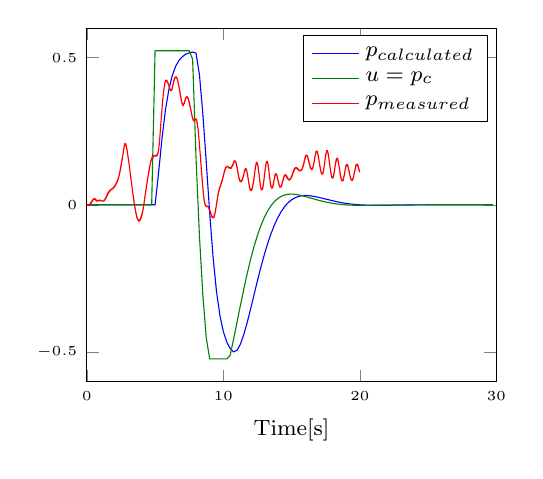
\begin{tikzpicture}

\begin{axis}[%
width = 5.2cm,
at={(0.758in,0.488in)},
scale only axis,
xmin=0,
xmax=30,
xlabel={\footnotesize{Time[s]}},
ymin=-0.6,
ymax=0.6,
ticklabel style = {font=\tiny},
axis background/.style={fill=white},
legend style={legend cell align=left, align=left, draw=black, font = \footnotesize}
]
\addplot [color=blue]
  table[row sep=crcr]{%
0	0\\
5	0\\
5.25	0.106028752058656\\
5.5	0.222660379323177\\
5.75	0.318881471816407\\
6	0.389443606311442\\
6.25	0.437955073776777\\
6.5	0.469972642303901\\
6.75	0.490517248775472\\
7	0.503431001414743\\
7.25	0.511421385860295\\
7.5	0.51630439857702\\
7.75	0.519258621270637\\
8	0.515203257617205\\
8.25	0.442077494057866\\
8.5	0.308917942206627\\
8.75	0.143857437412503\\
9	-0.026642171347433\\
9.25	-0.178852015358114\\
9.5	-0.294706712119982\\
9.75	-0.376103400744807\\
10	-0.430593712461647\\
10.25	-0.465910557041166\\
10.5	-0.488275766784287\\
10.75	-0.499764190883543\\
11	-0.494606006688155\\
11.25	-0.473847629784874\\
11.5	-0.440912018084063\\
11.75	-0.399653357456756\\
12	-0.353578675828111\\
12.5	-0.2579493548984\\
12.75	-0.212334914967485\\
13	-0.169924129646144\\
13.25	-0.131479200507158\\
13.5	-0.0974290818102865\\
13.75	-0.0679368059974763\\
14	-0.0429635308410177\\
14.25	-0.0223192342127767\\
14.5	-0.00570663885556044\\
14.75	0.00724201878417929\\
15	0.0169351049858726\\
15.25	0.0237983108610464\\
15.5	0.0282551996218636\\
15.75	0.03071226238756\\
16	0.0315508532381052\\
16.25	0.0311187961644848\\
16.5	0.029725886927416\\
16.75	0.0276432096833794\\
17.25	0.0222957734120826\\
18.25	0.0110954475341742\\
18.75	0.00659868322602009\\
19.25	0.003167897261946\\
19.75	0.000778241874598962\\
20.25	-0.000708334391688936\\
21	-0.00165871055146738\\
22	-0.00152183353077362\\
25	0\\
29.75	0\\
};
\addlegendentry{$p_{\text{calculated}}$}

\addplot [color=black!50!green]
  table[row sep=crcr]{%
0	0\\
4.75	0\\
5	0.523598775598298\\
7.5	0.523598775598298\\
7.75	0.494819035995317\\
8	0.160146388213864\\
8.25	-0.106263288038623\\
8.5	-0.307278306480395\\
8.75	-0.451544073993496\\
9	-0.523598775598298\\
10.25	-0.523598775598298\\
10.5	-0.511598967534702\\
10.75	-0.457129956387682\\
11.25	-0.342212060957365\\
11.5	-0.286365657156612\\
11.75	-0.233757373314109\\
12	-0.185424703030396\\
12.25	-0.142014857669654\\
12.5	-0.10385960931001\\
12.75	-0.0710390273514889\\
13	-0.0434270107361172\\
13.25	-0.0207605455327027\\
13.5	-0.0026532057262969\\
13.75	0.0113316469560196\\
14	0.0216778562869422\\
14.25	0.0288792627115377\\
14.5	0.0334210033379279\\
14.75	0.035766054664041\\
15	0.0363476842410009\\
15.25	0.0355551947305592\\
15.5	0.0337310214270481\\
15.75	0.0311830246785298\\
16.25	0.0248856506222559\\
17	0.0150402814094832\\
17.5	0.00942686961320049\\
18	0.00499923826903981\\
18.5	0.0017986264491725\\
19	-0.000289665822503338\\
19.5	-0.0014745362668549\\
20.25	-0.00203640858014609\\
21.25	-0.00156935527676438\\
23.5	-8.39090499056283e-05\\
26.25	0\\
29.75	0\\
};
\addlegendentry{$u = p_c$}

\addplot [color=red, forget plot]
  table[row sep=crcr]{%
0	0\\
0.0519999999999996	0\\
0.0539999999999985	-0.00153398078788669\\
0.161999999999999	-0.00153398078788669\\
0.164000000000001	0\\
0.207999999999998	0\\
0.210000000000001	0.00153398078788669\\
0.239999999999998	0.00153398078788669\\
0.242000000000001	0.00306796157576983\\
0.257999999999999	0.00306796157576983\\
0.260000000000002	0.00460194236365652\\
0.286000000000001	0.00460194236365652\\
0.288	0.00613592315154321\\
0.303999999999998	0.00613592315154321\\
0.306000000000001	0.0076699039394299\\
0.329999999999998	0.0076699039394299\\
0.332000000000001	0.00920388472731304\\
0.346	0.00920388472731304\\
0.347999999999999	0.0107378655151997\\
0.352	0.0107378655151997\\
0.353999999999999	0.00920388472731304\\
0.356000000000002	0.00920388472731304\\
0.358000000000001	0.0107378655151997\\
0.359999999999999	0.0107378655151997\\
0.361999999999998	0.0122718463030864\\
0.364000000000001	0.0122718463030864\\
0.366	0.0107378655151997\\
0.367999999999999	0.0107378655151997\\
0.370000000000001	0.0122718463030864\\
0.373999999999999	0.0122718463030864\\
0.376000000000001	0.0138058270909696\\
0.378	0.0122718463030864\\
0.384	0.0122718463030864\\
0.385999999999999	0.0138058270909696\\
0.390000000000001	0.0138058270909696\\
0.391999999999999	0.0122718463030864\\
0.393999999999998	0.0122718463030864\\
0.396000000000001	0.0138058270909696\\
0.408000000000001	0.0138058270909696\\
0.41	0.0153398078788562\\
0.431999999999999	0.0153398078788562\\
0.434000000000001	0.0168737886667429\\
0.454000000000001	0.0168737886667429\\
0.456	0.0184077694546261\\
0.460000000000001	0.0184077694546261\\
0.462	0.0168737886667429\\
0.463999999999999	0.0168737886667429\\
0.466000000000001	0.0184077694546261\\
0.488	0.0184077694546261\\
0.489999999999998	0.0199417502425128\\
0.492000000000001	0.0199417502425128\\
0.494	0.0184077694546261\\
0.498000000000001	0.0184077694546261\\
0.5	0.0199417502425128\\
0.501999999999999	0.0199417502425128\\
0.504000000000001	0.0184077694546261\\
0.507999999999999	0.0184077694546261\\
0.510000000000002	0.0199417502425128\\
0.516000000000002	0.0199417502425128\\
0.518000000000001	0.0184077694546261\\
0.52	0.0199417502425128\\
0.552	0.0199417502425128\\
0.553999999999998	0.0214757310303995\\
0.556000000000001	0.0214757310303995\\
0.558	0.0199417502425128\\
0.562000000000001	0.0199417502425128\\
0.564	0.0214757310303995\\
0.565999999999999	0.0214757310303995\\
0.568000000000001	0.0199417502425128\\
0.597999999999999	0.0199417502425128\\
0.600000000000001	0.0184077694546261\\
0.602	0.0184077694546261\\
0.603999999999999	0.0199417502425128\\
0.608000000000001	0.0199417502425128\\
0.609999999999999	0.0184077694546261\\
0.611999999999998	0.0184077694546261\\
0.614000000000001	0.0199417502425128\\
0.617999999999999	0.0199417502425128\\
0.620000000000001	0.0184077694546261\\
0.623999999999999	0.0184077694546261\\
0.626000000000001	0.0199417502425128\\
0.628	0.0199417502425128\\
0.629999999999999	0.0184077694546261\\
0.634	0.0184077694546261\\
0.635999999999999	0.0199417502425128\\
0.638000000000002	0.0199417502425128\\
0.641999999999999	0.0168737886667429\\
0.643999999999998	0.0168737886667429\\
0.646000000000001	0.0184077694546261\\
0.648	0.0184077694546261\\
0.649999999999999	0.0168737886667429\\
0.654	0.0168737886667429\\
0.655999999999999	0.0184077694546261\\
0.658000000000001	0.0184077694546261\\
0.661999999999999	0.0153398078788562\\
0.664000000000001	0.0153398078788562\\
0.666	0.0168737886667429\\
0.670000000000002	0.0168737886667429\\
0.672000000000001	0.0153398078788562\\
0.675999999999998	0.0153398078788562\\
0.678000000000001	0.0168737886667429\\
0.68	0.0168737886667429\\
0.681999999999999	0.0153398078788562\\
0.692	0.0153398078788562\\
0.693999999999999	0.0138058270909696\\
0.696000000000002	0.0138058270909696\\
0.698	0.0153398078788562\\
0.699999999999999	0.0153398078788562\\
0.702000000000002	0.0138058270909696\\
0.73	0.0138058270909696\\
0.731999999999999	0.0122718463030864\\
0.736000000000001	0.0122718463030864\\
0.738	0.0138058270909696\\
0.739999999999998	0.0138058270909696\\
0.742000000000001	0.0122718463030864\\
0.776	0.0122718463030864\\
0.777999999999999	0.0138058270909696\\
0.780000000000001	0.0138058270909696\\
0.782	0.0122718463030864\\
0.812000000000001	0.0122718463030864\\
0.814	0.0138058270909696\\
0.864000000000001	0.0138058270909696\\
0.866	0.0153398078788562\\
0.981999999999999	0.0153398078788562\\
0.984000000000002	0.0138058270909696\\
1.08	0.0138058270909696\\
1.082	0.0122718463030864\\
1.226	0.0122718463030864\\
1.228	0.0138058270909696\\
1.27	0.0138058270909696\\
1.272	0.0153398078788562\\
1.3	0.0153398078788562\\
1.302	0.0168737886667429\\
1.316	0.0168737886667429\\
1.318	0.0184077694546261\\
1.342	0.0184077694546261\\
1.344	0.0199417502425128\\
1.364	0.0199417502425128\\
1.366	0.0214757310303995\\
1.378	0.0214757310303995\\
1.38	0.0230097118182861\\
1.382	0.0230097118182861\\
1.384	0.0214757310303995\\
1.388	0.0214757310303995\\
1.39	0.0230097118182861\\
1.4	0.0230097118182861\\
1.402	0.0245436926061693\\
1.412	0.0245436926061693\\
1.414	0.026077673394056\\
1.416	0.026077673394056\\
1.418	0.0245436926061693\\
1.42	0.0245436926061693\\
1.422	0.026077673394056\\
1.424	0.026077673394056\\
1.426	0.0276116541819427\\
1.428	0.026077673394056\\
1.432	0.026077673394056\\
1.434	0.0276116541819427\\
1.444	0.0276116541819427\\
1.446	0.0291456349698258\\
1.456	0.0291456349698258\\
1.458	0.0306796157577125\\
1.46	0.0306796157577125\\
1.462	0.0291456349698258\\
1.464	0.0291456349698258\\
1.468	0.0322135965455992\\
1.47	0.0322135965455992\\
1.472	0.0306796157577125\\
1.476	0.0306796157577125\\
1.48	0.0337475773334859\\
1.482	0.0322135965455992\\
1.486	0.0322135965455992\\
1.49	0.035281558121369\\
1.494	0.0322135965455992\\
1.496	0.0322135965455992\\
1.5	0.035281558121369\\
1.502	0.035281558121369\\
1.504	0.0337475773334859\\
1.506	0.0337475773334859\\
1.51	0.0368155389092557\\
1.512	0.0368155389092557\\
1.514	0.035281558121369\\
1.518	0.035281558121369\\
1.52	0.0368155389092557\\
1.526	0.0368155389092557\\
1.528	0.035281558121369\\
1.532	0.0383495196971424\\
1.534	0.0383495196971424\\
1.536	0.0368155389092557\\
1.538	0.0368155389092557\\
1.542	0.0398835004850255\\
1.544	0.0398835004850255\\
1.546	0.0383495196971424\\
1.55	0.0383495196971424\\
1.552	0.0398835004850255\\
1.558	0.0398835004850255\\
1.56	0.0383495196971424\\
1.564	0.0414174812729122\\
1.566	0.0414174812729122\\
1.568	0.0398835004850255\\
1.572	0.0398835004850255\\
1.576	0.0429514620607989\\
1.578	0.0414174812729122\\
1.584	0.0414174812729122\\
1.586	0.0429514620607989\\
1.59	0.0429514620607989\\
1.592	0.0414174812729122\\
1.594	0.0414174812729122\\
1.596	0.0429514620607989\\
1.606	0.0429514620607989\\
1.608	0.0444854428486821\\
1.61	0.0429514620607989\\
1.614	0.0429514620607989\\
1.616	0.0444854428486821\\
1.62	0.0444854428486821\\
1.622	0.0429514620607989\\
1.624	0.0429514620607989\\
1.626	0.0444854428486821\\
1.638	0.0444854428486821\\
1.64	0.0460194236365687\\
1.642	0.0460194236365687\\
1.644	0.0444854428486821\\
1.646	0.0444854428486821\\
1.648	0.0460194236365687\\
1.67	0.0460194236365687\\
1.672	0.0475534044244554\\
1.702	0.0475534044244554\\
1.704	0.0490873852123421\\
1.738	0.0490873852123421\\
1.74	0.0506213660002253\\
1.742	0.0490873852123421\\
1.746	0.0490873852123421\\
1.748	0.0506213660002253\\
1.77	0.0506213660002253\\
1.772	0.052155346788112\\
1.776	0.052155346788112\\
1.778	0.0506213660002253\\
1.78	0.0506213660002253\\
1.782	0.052155346788112\\
1.826	0.052155346788112\\
1.828	0.0536893275759986\\
1.858	0.0536893275759986\\
1.86	0.0552233083638818\\
1.9	0.0552233083638818\\
1.902	0.0567572891517685\\
1.936	0.0567572891517685\\
1.938	0.0582912699396552\\
1.97	0.0582912699396552\\
1.972	0.0598252507275383\\
1.998	0.0598252507275383\\
2	0.061359231515425\\
2.02	0.061359231515425\\
2.022	0.0628932123033117\\
2.044	0.0628932123033117\\
2.046	0.0644271930911984\\
2.068	0.0644271930911984\\
2.07	0.0659611738790815\\
2.086	0.0659611738790815\\
2.088	0.0674951546669682\\
2.11	0.0674951546669682\\
2.112	0.0690291354548549\\
2.13	0.0690291354548549\\
2.132	0.070563116242738\\
2.148	0.070563116242738\\
2.15	0.0720970970306247\\
2.162	0.0720970970306247\\
2.164	0.0736310778185114\\
2.176	0.0736310778185114\\
2.178	0.0751650586063981\\
2.188	0.0751650586063981\\
2.19	0.0766990393942812\\
2.194	0.0766990393942812\\
2.196	0.0751650586063981\\
2.198	0.0751650586063981\\
2.2	0.0766990393942812\\
2.202	0.0766990393942812\\
2.204	0.0782330201821679\\
2.206	0.0766990393942812\\
2.21	0.0766990393942812\\
2.212	0.0782330201821679\\
2.214	0.0782330201821679\\
2.216	0.0797670009700546\\
2.218	0.0797670009700546\\
2.22	0.0782330201821679\\
2.224	0.0782330201821679\\
2.226	0.0797670009700546\\
2.236	0.0797670009700546\\
2.238	0.0813009817579378\\
2.248	0.0813009817579378\\
2.25	0.0828349625458245\\
2.26	0.0828349625458245\\
2.262	0.0843689433337111\\
2.272	0.0843689433337111\\
2.274	0.0859029241215943\\
2.284	0.0859029241215943\\
2.286	0.087436904909481\\
2.296	0.087436904909481\\
2.298	0.0889708856973677\\
2.312	0.0889708856973677\\
2.314	0.0905048664852544\\
2.316	0.0905048664852544\\
2.318	0.0920388472731375\\
2.324	0.0920388472731375\\
2.326	0.0935728280610242\\
2.336	0.0935728280610242\\
2.338	0.0951068088489109\\
2.346	0.0951068088489109\\
2.348	0.096640789636794\\
2.35	0.096640789636794\\
2.352	0.0981747704246807\\
2.358	0.0981747704246807\\
2.36	0.0997087512125674\\
2.366	0.0997087512125674\\
2.368	0.101242732000454\\
2.376	0.101242732000454\\
2.38	0.104310693576224\\
2.388	0.104310693576224\\
2.39	0.105844674364111\\
2.398	0.105844674364111\\
2.402	0.10891263593988\\
2.404	0.10891263593988\\
2.406	0.107378655151994\\
2.408	0.107378655151994\\
2.412	0.110446616727767\\
2.42	0.110446616727767\\
2.424	0.113514578303537\\
2.426	0.11198059751565\\
2.428	0.11198059751565\\
2.434	0.11658253987931\\
2.436	0.115048559091424\\
2.44	0.115048559091424\\
2.442	0.118116520667193\\
2.446	0.118116520667193\\
2.448	0.11658253987931\\
2.454	0.121184482242967\\
2.456	0.121184482242967\\
2.458	0.11965050145508\\
2.46	0.11965050145508\\
2.462	0.12271846303085\\
2.464	0.124252443818737\\
2.466	0.124252443818737\\
2.468	0.12271846303085\\
2.47	0.12271846303085\\
2.476	0.127320405394507\\
2.478	0.125786424606623\\
2.482	0.125786424606623\\
2.484	0.128854386182393\\
2.488	0.128854386182393\\
2.49	0.127320405394507\\
2.492	0.128854386182393\\
2.494	0.131922347758167\\
2.498	0.131922347758167\\
2.5	0.13038836697028\\
2.502	0.13038836697028\\
2.504	0.13345632854605\\
2.506	0.134990309333936\\
2.508	0.134990309333936\\
2.51	0.13345632854605\\
2.512	0.13345632854605\\
2.514	0.136524290121823\\
2.518	0.136524290121823\\
2.52	0.134990309333936\\
2.522	0.136524290121823\\
2.524	0.139592251697593\\
2.528	0.139592251697593\\
2.53	0.138058270909706\\
2.536	0.142660213273366\\
2.538	0.142660213273366\\
2.54	0.14112623248548\\
2.542	0.14112623248548\\
2.544	0.144194194061249\\
2.546	0.145728174849136\\
2.548	0.145728174849136\\
2.55	0.144194194061249\\
2.552	0.144194194061249\\
2.558	0.148796136424906\\
2.56	0.145728174849136\\
2.568	0.151864098000679\\
2.57	0.148796136424906\\
2.572	0.150330117212793\\
2.574	0.150330117212793\\
2.576	0.153398078788562\\
2.578	0.153398078788562\\
2.58	0.151864098000679\\
2.582	0.151864098000679\\
2.584	0.153398078788562\\
2.586	0.156466040364336\\
2.588	0.156466040364336\\
2.59	0.154932059576449\\
2.594	0.154932059576449\\
2.596	0.159534001940106\\
2.598	0.159534001940106\\
2.6	0.158000021152223\\
2.604	0.158000021152223\\
2.606	0.161067982727992\\
2.608	0.162601963515879\\
2.61	0.161067982727992\\
2.614	0.161067982727992\\
2.616	0.164135944303762\\
2.618	0.165669925091649\\
2.62	0.165669925091649\\
2.622	0.162601963515879\\
2.624	0.164135944303762\\
2.626	0.167203905879536\\
2.628	0.167203905879536\\
2.63	0.168737886667422\\
2.632	0.165669925091649\\
2.64	0.171805848243192\\
2.642	0.168737886667422\\
2.65	0.174873809818962\\
2.652	0.171805848243192\\
2.66	0.177941771394735\\
2.662	0.174873809818962\\
2.664	0.174873809818962\\
2.666	0.177941771394735\\
2.668	0.179475752182618\\
2.67	0.179475752182618\\
2.672	0.177941771394735\\
2.674	0.177941771394735\\
2.676	0.179475752182618\\
2.678	0.182543713758392\\
2.68	0.182543713758392\\
2.682	0.181009732970505\\
2.684	0.181009732970505\\
2.686	0.182543713758392\\
2.688	0.185611675334162\\
2.69	0.185611675334162\\
2.692	0.184077694546279\\
2.694	0.184077694546279\\
2.696	0.185611675334162\\
2.698	0.188679636909935\\
2.7	0.188679636909935\\
2.702	0.187145656122048\\
2.706	0.187145656122048\\
2.708	0.190213617697818\\
2.71	0.191747598485705\\
2.712	0.190213617697818\\
2.716	0.190213617697818\\
2.718	0.193281579273592\\
2.722	0.193281579273592\\
2.724	0.191747598485705\\
2.726	0.193281579273592\\
2.728	0.196349540849361\\
2.732	0.196349540849361\\
2.734	0.194815560061475\\
2.736	0.194815560061475\\
2.738	0.197883521637248\\
2.74	0.199417502425135\\
2.742	0.199417502425135\\
2.744	0.197883521637248\\
2.746	0.197883521637248\\
2.75	0.200951483213018\\
2.758	0.200951483213018\\
2.762	0.204019444788791\\
2.764	0.202485464000905\\
2.768	0.202485464000905\\
2.77	0.205553425576674\\
2.772	0.205553425576674\\
2.774	0.204019444788791\\
2.778	0.204019444788791\\
2.782	0.207087406364561\\
2.784	0.205553425576674\\
2.788	0.205553425576674\\
2.79	0.207087406364561\\
2.8	0.207087406364561\\
2.802	0.208621387152448\\
2.806	0.208621387152448\\
2.808	0.207087406364561\\
2.81	0.207087406364561\\
2.812	0.208621387152448\\
2.828	0.208621387152448\\
2.83	0.207087406364561\\
2.842	0.207087406364561\\
2.844	0.205553425576674\\
2.85	0.205553425576674\\
2.852	0.207087406364561\\
2.856	0.204019444788791\\
2.866	0.204019444788791\\
2.868	0.202485464000905\\
2.876	0.202485464000905\\
2.878	0.200951483213018\\
2.88	0.200951483213018\\
2.882	0.199417502425135\\
2.89	0.199417502425135\\
2.892	0.197883521637248\\
2.896	0.197883521637248\\
2.898	0.196349540849361\\
2.904	0.196349540849361\\
2.906	0.194815560061475\\
2.91	0.194815560061475\\
2.912	0.193281579273592\\
2.916	0.193281579273592\\
2.918	0.191747598485705\\
2.922	0.191747598485705\\
2.924	0.190213617697818\\
2.928	0.190213617697818\\
2.93	0.188679636909935\\
2.934	0.188679636909935\\
2.936	0.187145656122048\\
2.94	0.187145656122048\\
2.942	0.185611675334162\\
2.944	0.185611675334162\\
2.946	0.184077694546279\\
2.952	0.184077694546279\\
2.954	0.182543713758392\\
2.956	0.182543713758392\\
2.958	0.181009732970505\\
2.962	0.181009732970505\\
2.964	0.179475752182618\\
2.966	0.179475752182618\\
2.968	0.177941771394735\\
2.972	0.177941771394735\\
2.974	0.176407790606849\\
2.976	0.176407790606849\\
2.978	0.174873809818962\\
2.982	0.174873809818962\\
2.984	0.173339829031079\\
2.988	0.173339829031079\\
2.99	0.171805848243192\\
2.992	0.171805848243192\\
2.994	0.170271867455305\\
2.998	0.170271867455305\\
3	0.168737886667422\\
3.002	0.168737886667422\\
3.004	0.167203905879536\\
3.006	0.167203905879536\\
3.008	0.165669925091649\\
3.012	0.165669925091649\\
3.014	0.164135944303762\\
3.016	0.164135944303762\\
3.018	0.162601963515879\\
3.022	0.162601963515879\\
3.024	0.161067982727992\\
3.026	0.161067982727992\\
3.028	0.159534001940106\\
3.032	0.159534001940106\\
3.034	0.158000021152223\\
3.036	0.158000021152223\\
3.038	0.156466040364336\\
3.04	0.156466040364336\\
3.042	0.154932059576449\\
3.044	0.154932059576449\\
3.046	0.153398078788562\\
3.05	0.153398078788562\\
3.052	0.151864098000679\\
3.054	0.151864098000679\\
3.056	0.150330117212793\\
3.06	0.150330117212793\\
3.062	0.148796136424906\\
3.064	0.148796136424906\\
3.066	0.147262155637023\\
3.068	0.147262155637023\\
3.07	0.145728174849136\\
3.072	0.145728174849136\\
3.074	0.144194194061249\\
3.076	0.144194194061249\\
3.078	0.142660213273366\\
3.082	0.142660213273366\\
3.084	0.14112623248548\\
3.086	0.14112623248548\\
3.088	0.139592251697593\\
3.09	0.139592251697593\\
3.092	0.138058270909706\\
3.096	0.138058270909706\\
3.098	0.136524290121823\\
3.1	0.136524290121823\\
3.102	0.134990309333936\\
3.104	0.134990309333936\\
3.106	0.13345632854605\\
3.108	0.13345632854605\\
3.11	0.131922347758167\\
3.112	0.131922347758167\\
3.114	0.13038836697028\\
3.118	0.13038836697028\\
3.12	0.128854386182393\\
3.122	0.128854386182393\\
3.124	0.127320405394507\\
3.126	0.127320405394507\\
3.128	0.125786424606623\\
3.132	0.125786424606623\\
3.136	0.12271846303085\\
3.14	0.12271846303085\\
3.142	0.121184482242967\\
3.144	0.121184482242967\\
3.146	0.11965050145508\\
3.148	0.11965050145508\\
3.15	0.118116520667193\\
3.152	0.118116520667193\\
3.154	0.11658253987931\\
3.156	0.11658253987931\\
3.158	0.115048559091424\\
3.16	0.115048559091424\\
3.162	0.113514578303537\\
3.166	0.113514578303537\\
3.168	0.11198059751565\\
3.17	0.11198059751565\\
3.172	0.110446616727767\\
3.174	0.110446616727767\\
3.176	0.10891263593988\\
3.178	0.10891263593988\\
3.18	0.107378655151994\\
3.182	0.107378655151994\\
3.184	0.105844674364111\\
3.186	0.105844674364111\\
3.188	0.104310693576224\\
3.19	0.104310693576224\\
3.192	0.102776712788337\\
3.194	0.102776712788337\\
3.196	0.101242732000454\\
3.198	0.101242732000454\\
3.2	0.0997087512125674\\
3.202	0.0997087512125674\\
3.204	0.0981747704246807\\
3.208	0.0981747704246807\\
3.21	0.096640789636794\\
3.212	0.096640789636794\\
3.214	0.0951068088489109\\
3.216	0.0951068088489109\\
3.218	0.0935728280610242\\
3.22	0.0935728280610242\\
3.222	0.0920388472731375\\
3.224	0.0920388472731375\\
3.226	0.0905048664852544\\
3.228	0.0905048664852544\\
3.23	0.0889708856973677\\
3.232	0.0889708856973677\\
3.234	0.087436904909481\\
3.236	0.087436904909481\\
3.238	0.0859029241215943\\
3.242	0.0859029241215943\\
3.244	0.0843689433337111\\
3.246	0.0843689433337111\\
3.248	0.0828349625458245\\
3.25	0.0828349625458245\\
3.252	0.0813009817579378\\
3.254	0.0813009817579378\\
3.256	0.0797670009700546\\
3.258	0.0797670009700546\\
3.26	0.0782330201821679\\
3.262	0.0782330201821679\\
3.264	0.0766990393942812\\
3.268	0.0766990393942812\\
3.27	0.0751650586063981\\
3.272	0.0751650586063981\\
3.274	0.0736310778185114\\
3.276	0.0736310778185114\\
3.278	0.0720970970306247\\
3.28	0.0720970970306247\\
3.282	0.070563116242738\\
3.284	0.070563116242738\\
3.286	0.0690291354548549\\
3.288	0.0690291354548549\\
3.29	0.0674951546669682\\
3.294	0.0674951546669682\\
3.296	0.0659611738790815\\
3.298	0.0659611738790815\\
3.302	0.0628932123033117\\
3.304	0.0628932123033117\\
3.306	0.061359231515425\\
3.31	0.061359231515425\\
3.312	0.0598252507275383\\
3.314	0.0598252507275383\\
3.316	0.0582912699396552\\
3.318	0.0582912699396552\\
3.32	0.0567572891517685\\
3.322	0.0567572891517685\\
3.324	0.0552233083638818\\
3.326	0.0552233083638818\\
3.328	0.0536893275759986\\
3.332	0.0536893275759986\\
3.334	0.052155346788112\\
3.336	0.052155346788112\\
3.338	0.0506213660002253\\
3.34	0.0506213660002253\\
3.342	0.0490873852123421\\
3.344	0.0490873852123421\\
3.346	0.0475534044244554\\
3.348	0.0475534044244554\\
3.35	0.0460194236365687\\
3.354	0.0460194236365687\\
3.356	0.0444854428486821\\
3.358	0.0444854428486821\\
3.36	0.0429514620607989\\
3.364	0.0429514620607989\\
3.368	0.0398835004850255\\
3.372	0.0398835004850255\\
3.374	0.0383495196971424\\
3.376	0.0383495196971424\\
3.378	0.0368155389092557\\
3.38	0.0368155389092557\\
3.382	0.035281558121369\\
3.384	0.035281558121369\\
3.386	0.0337475773334859\\
3.39	0.0337475773334859\\
3.392	0.0322135965455992\\
3.394	0.0322135965455992\\
3.396	0.0306796157577125\\
3.4	0.0306796157577125\\
3.402	0.0291456349698258\\
3.404	0.0291456349698258\\
3.406	0.0276116541819427\\
3.408	0.0276116541819427\\
3.41	0.026077673394056\\
3.412	0.026077673394056\\
3.414	0.0245436926061693\\
3.416	0.0245436926061693\\
3.418	0.0230097118182861\\
3.42	0.0230097118182861\\
3.422	0.0214757310303995\\
3.426	0.0214757310303995\\
3.428	0.0199417502425128\\
3.432	0.0199417502425128\\
3.434	0.0184077694546261\\
3.436	0.0184077694546261\\
3.438	0.0168737886667429\\
3.442	0.0168737886667429\\
3.444	0.0153398078788562\\
3.446	0.0153398078788562\\
3.448	0.0138058270909696\\
3.45	0.0138058270909696\\
3.452	0.0122718463030864\\
3.456	0.0122718463030864\\
3.458	0.0107378655151997\\
3.46	0.0107378655151997\\
3.462	0.00920388472731304\\
3.464	0.00920388472731304\\
3.466	0.0076699039394299\\
3.47	0.0076699039394299\\
3.472	0.00613592315154321\\
3.476	0.00613592315154321\\
3.478	0.00460194236365652\\
3.48	0.00460194236365652\\
3.482	0.00306796157576983\\
3.484	0.00306796157576983\\
3.486	0.00153398078788669\\
3.49	0.00153398078788669\\
3.492	0\\
3.496	0\\
3.498	-0.00153398078788669\\
3.5	-0.00153398078788669\\
3.502	-0.00306796157576983\\
3.506	-0.00306796157576983\\
3.508	-0.00460194236365652\\
3.51	-0.00460194236365652\\
3.512	-0.00613592315154321\\
3.516	-0.00613592315154321\\
3.518	-0.0076699039394299\\
3.522	-0.0076699039394299\\
3.524	-0.00920388472731304\\
3.528	-0.00920388472731304\\
3.53	-0.0107378655151997\\
3.532	-0.0107378655151997\\
3.534	-0.0122718463030864\\
3.538	-0.0122718463030864\\
3.54	-0.0138058270909696\\
3.544	-0.0138058270909696\\
3.546	-0.0153398078788562\\
3.55	-0.0153398078788562\\
3.552	-0.0168737886667429\\
3.556	-0.0168737886667429\\
3.558	-0.0184077694546261\\
3.562	-0.0184077694546261\\
3.564	-0.0199417502425128\\
3.568	-0.0199417502425128\\
3.57	-0.0214757310303995\\
3.574	-0.0214757310303995\\
3.576	-0.0230097118182861\\
3.58	-0.0230097118182861\\
3.582	-0.0245436926061693\\
3.586	-0.0245436926061693\\
3.588	-0.026077673394056\\
3.592	-0.026077673394056\\
3.594	-0.0276116541819427\\
3.6	-0.0276116541819427\\
3.602	-0.0291456349698258\\
3.606	-0.0291456349698258\\
3.608	-0.0306796157577125\\
3.614	-0.0306796157577125\\
3.616	-0.0322135965455992\\
3.62	-0.0322135965455992\\
3.622	-0.0337475773334859\\
3.63	-0.0337475773334859\\
3.632	-0.035281558121369\\
3.636	-0.035281558121369\\
3.638	-0.0368155389092557\\
3.644	-0.0368155389092557\\
3.646	-0.0383495196971424\\
3.652	-0.0383495196971424\\
3.654	-0.0398835004850255\\
3.662	-0.0398835004850255\\
3.664	-0.0414174812729122\\
3.674	-0.0414174812729122\\
3.676	-0.0429514620607989\\
3.682	-0.0429514620607989\\
3.684	-0.0444854428486821\\
3.69	-0.0444854428486821\\
3.692	-0.0460194236365687\\
3.704	-0.0460194236365687\\
3.706	-0.0475534044244554\\
3.716	-0.0475534044244554\\
3.718	-0.0490873852123421\\
3.73	-0.0490873852123421\\
3.732	-0.0506213660002253\\
3.752	-0.0506213660002253\\
3.754	-0.052155346788112\\
3.766	-0.052155346788112\\
3.768	-0.0536893275759986\\
3.772	-0.0536893275759986\\
3.774	-0.052155346788112\\
3.776	-0.052155346788112\\
3.778	-0.0536893275759986\\
3.792	-0.0536893275759986\\
3.794	-0.0552233083638818\\
3.796	-0.0536893275759986\\
3.802	-0.0536893275759986\\
3.804	-0.0552233083638818\\
3.808	-0.0552233083638818\\
3.81	-0.0536893275759986\\
3.814	-0.0536893275759986\\
3.816	-0.0552233083638818\\
3.82	-0.0552233083638818\\
3.822	-0.0536893275759986\\
3.826	-0.0536893275759986\\
3.828	-0.0552233083638818\\
3.83	-0.0552233083638818\\
3.832	-0.0536893275759986\\
3.838	-0.0536893275759986\\
3.84	-0.0552233083638818\\
3.842	-0.0552233083638818\\
3.844	-0.0536893275759986\\
3.85	-0.0536893275759986\\
3.852	-0.0552233083638818\\
3.854	-0.0536893275759986\\
3.866	-0.0536893275759986\\
3.868	-0.052155346788112\\
3.87	-0.052155346788112\\
3.872	-0.0536893275759986\\
3.874	-0.0536893275759986\\
3.876	-0.052155346788112\\
3.896	-0.052155346788112\\
3.898	-0.0506213660002253\\
3.902	-0.0506213660002253\\
3.904	-0.052155346788112\\
3.906	-0.052155346788112\\
3.91	-0.0490873852123421\\
3.912	-0.0490873852123421\\
3.914	-0.0506213660002253\\
3.916	-0.0506213660002253\\
3.918	-0.0490873852123421\\
3.928	-0.0490873852123421\\
3.93	-0.0475534044244554\\
3.934	-0.0475534044244554\\
3.936	-0.0490873852123421\\
3.938	-0.0490873852123421\\
3.94	-0.0460194236365687\\
3.944	-0.0460194236365687\\
3.946	-0.0475534044244554\\
3.948	-0.0475534044244554\\
3.952	-0.0444854428486821\\
3.954	-0.0444854428486821\\
3.956	-0.0460194236365687\\
3.958	-0.0460194236365687\\
3.962	-0.0429514620607989\\
3.964	-0.0429514620607989\\
3.966	-0.0460194236365687\\
3.968	-0.0444854428486821\\
3.97	-0.0444854428486821\\
3.972	-0.0414174812729122\\
3.974	-0.0414174812729122\\
3.976	-0.0429514620607989\\
3.98	-0.0429514620607989\\
3.982	-0.0398835004850255\\
3.984	-0.0398835004850255\\
3.988	-0.0429514620607989\\
3.99	-0.0414174812729122\\
3.992	-0.0383495196971424\\
3.994	-0.0383495196971424\\
3.998	-0.0414174812729122\\
4.004	-0.0368155389092557\\
4.006	-0.0368155389092557\\
4.008	-0.0398835004850255\\
4.014	-0.035281558121369\\
4.016	-0.035281558121369\\
4.018	-0.0368155389092557\\
4.022	-0.0368155389092557\\
4.024	-0.0337475773334859\\
4.026	-0.0337475773334859\\
4.028	-0.035281558121369\\
4.032	-0.035281558121369\\
4.034	-0.0322135965455992\\
4.036	-0.0322135965455992\\
4.038	-0.0337475773334859\\
4.042	-0.0337475773334859\\
4.044	-0.0306796157577125\\
4.048	-0.0306796157577125\\
4.05	-0.0322135965455992\\
4.052	-0.0322135965455992\\
4.054	-0.0291456349698258\\
4.058	-0.0291456349698258\\
4.06	-0.0306796157577125\\
4.066	-0.026077673394056\\
4.068	-0.0276116541819427\\
4.072	-0.0276116541819427\\
4.076	-0.0245436926061693\\
4.08	-0.0245436926061693\\
4.082	-0.026077673394056\\
4.086	-0.0230097118182861\\
4.092	-0.0230097118182861\\
4.094	-0.0214757310303995\\
4.096	-0.0214757310303995\\
4.098	-0.0199417502425128\\
4.1	-0.0214757310303995\\
4.102	-0.0214757310303995\\
4.104	-0.0199417502425128\\
4.106	-0.0199417502425128\\
4.108	-0.0184077694546261\\
4.112	-0.0184077694546261\\
4.114	-0.0168737886667429\\
4.116	-0.0168737886667429\\
4.118	-0.0153398078788562\\
4.124	-0.0153398078788562\\
4.126	-0.0138058270909696\\
4.13	-0.0138058270909696\\
4.132	-0.0122718463030864\\
4.134	-0.0122718463030864\\
4.136	-0.0107378655151997\\
4.142	-0.0107378655151997\\
4.146	-0.0076699039394299\\
4.148	-0.0076699039394299\\
4.15	-0.00613592315154321\\
4.156	-0.00613592315154321\\
4.16	-0.00306796157576983\\
4.166	-0.00306796157576983\\
4.168	-0.00153398078788669\\
4.17	-0.00153398078788669\\
4.172	0\\
4.176	0\\
4.178	0.00153398078788669\\
4.18	0.00153398078788669\\
4.182	0.00306796157576983\\
4.184	0.00306796157576983\\
4.186	0.00460194236365652\\
4.19	0.00460194236365652\\
4.192	0.00613592315154321\\
4.194	0.00613592315154321\\
4.196	0.0076699039394299\\
4.198	0.0076699039394299\\
4.2	0.00920388472731304\\
4.204	0.00920388472731304\\
4.206	0.0107378655151997\\
4.208	0.0107378655151997\\
4.21	0.0122718463030864\\
4.214	0.0122718463030864\\
4.216	0.0138058270909696\\
4.218	0.0138058270909696\\
4.22	0.0153398078788562\\
4.222	0.0153398078788562\\
4.224	0.0168737886667429\\
4.228	0.0168737886667429\\
4.23	0.0184077694546261\\
4.232	0.0184077694546261\\
4.234	0.0199417502425128\\
4.236	0.0199417502425128\\
4.238	0.0214757310303995\\
4.242	0.0214757310303995\\
4.244	0.0230097118182861\\
4.246	0.0230097118182861\\
4.248	0.0245436926061693\\
4.252	0.0245436926061693\\
4.254	0.026077673394056\\
4.256	0.026077673394056\\
4.258	0.0276116541819427\\
4.26	0.0276116541819427\\
4.262	0.0291456349698258\\
4.266	0.0291456349698258\\
4.268	0.0306796157577125\\
4.27	0.0306796157577125\\
4.272	0.0322135965455992\\
4.276	0.0322135965455992\\
4.278	0.0337475773334859\\
4.28	0.0337475773334859\\
4.282	0.035281558121369\\
4.284	0.035281558121369\\
4.286	0.0368155389092557\\
4.288	0.0368155389092557\\
4.29	0.0383495196971424\\
4.292	0.0383495196971424\\
4.294	0.0398835004850255\\
4.298	0.0398835004850255\\
4.3	0.0414174812729122\\
4.302	0.0414174812729122\\
4.304	0.0429514620607989\\
4.308	0.0429514620607989\\
4.31	0.0444854428486821\\
4.312	0.0444854428486821\\
4.314	0.0460194236365687\\
4.316	0.0460194236365687\\
4.318	0.0475534044244554\\
4.32	0.0475534044244554\\
4.322	0.0490873852123421\\
4.326	0.0490873852123421\\
4.328	0.0506213660002253\\
4.332	0.0506213660002253\\
4.334	0.052155346788112\\
4.336	0.052155346788112\\
4.338	0.0536893275759986\\
4.342	0.0536893275759986\\
4.344	0.0552233083638818\\
4.346	0.0552233083638818\\
4.348	0.0567572891517685\\
4.35	0.0567572891517685\\
4.352	0.0582912699396552\\
4.356	0.0582912699396552\\
4.358	0.0598252507275383\\
4.36	0.0598252507275383\\
4.362	0.061359231515425\\
4.366	0.061359231515425\\
4.368	0.0628932123033117\\
4.37	0.0628932123033117\\
4.372	0.0644271930911984\\
4.376	0.0644271930911984\\
4.378	0.0659611738790815\\
4.38	0.0659611738790815\\
4.382	0.0674951546669682\\
4.386	0.0674951546669682\\
4.388	0.0690291354548549\\
4.39	0.0690291354548549\\
4.392	0.070563116242738\\
4.396	0.070563116242738\\
4.398	0.0720970970306247\\
4.4	0.0720970970306247\\
4.402	0.0736310778185114\\
4.406	0.0736310778185114\\
4.408	0.0751650586063981\\
4.412	0.0751650586063981\\
4.414	0.0766990393942812\\
4.416	0.0766990393942812\\
4.418	0.0782330201821679\\
4.422	0.0782330201821679\\
4.424	0.0797670009700546\\
4.426	0.0797670009700546\\
4.428	0.0813009817579378\\
4.432	0.0813009817579378\\
4.434	0.0828349625458245\\
4.436	0.0828349625458245\\
4.438	0.0843689433337111\\
4.442	0.0843689433337111\\
4.444	0.0859029241215943\\
4.448	0.0859029241215943\\
4.45	0.087436904909481\\
4.454	0.087436904909481\\
4.456	0.0889708856973677\\
4.458	0.0889708856973677\\
4.46	0.0905048664852544\\
4.464	0.0905048664852544\\
4.466	0.0920388472731375\\
4.468	0.0920388472731375\\
4.47	0.0935728280610242\\
4.474	0.0935728280610242\\
4.476	0.0951068088489109\\
4.48	0.0951068088489109\\
4.482	0.096640789636794\\
4.486	0.096640789636794\\
4.488	0.0981747704246807\\
4.49	0.0981747704246807\\
4.492	0.0997087512125674\\
4.496	0.0997087512125674\\
4.498	0.101242732000454\\
4.502	0.101242732000454\\
4.504	0.102776712788337\\
4.508	0.102776712788337\\
4.51	0.104310693576224\\
4.512	0.104310693576224\\
4.514	0.105844674364111\\
4.518	0.105844674364111\\
4.52	0.107378655151994\\
4.524	0.107378655151994\\
4.526	0.10891263593988\\
4.53	0.10891263593988\\
4.532	0.110446616727767\\
4.536	0.110446616727767\\
4.538	0.11198059751565\\
4.542	0.11198059751565\\
4.544	0.113514578303537\\
4.548	0.113514578303537\\
4.55	0.115048559091424\\
4.554	0.115048559091424\\
4.556	0.11658253987931\\
4.56	0.11658253987931\\
4.562	0.118116520667193\\
4.566	0.118116520667193\\
4.568	0.11965050145508\\
4.572	0.11965050145508\\
4.574	0.121184482242967\\
4.578	0.121184482242967\\
4.58	0.12271846303085\\
4.584	0.12271846303085\\
4.586	0.124252443818737\\
4.59	0.124252443818737\\
4.592	0.125786424606623\\
4.596	0.125786424606623\\
4.598	0.127320405394507\\
4.6	0.127320405394507\\
4.602	0.128854386182393\\
4.608	0.128854386182393\\
4.61	0.13038836697028\\
4.614	0.13038836697028\\
4.616	0.131922347758167\\
4.62	0.131922347758167\\
4.622	0.13345632854605\\
4.626	0.13345632854605\\
4.628	0.134990309333936\\
4.634	0.134990309333936\\
4.636	0.136524290121823\\
4.64	0.136524290121823\\
4.642	0.138058270909706\\
4.648	0.138058270909706\\
4.65	0.139592251697593\\
4.656	0.139592251697593\\
4.658	0.14112623248548\\
4.662	0.14112623248548\\
4.664	0.142660213273366\\
4.67	0.142660213273366\\
4.672	0.144194194061249\\
4.676	0.144194194061249\\
4.678	0.145728174849136\\
4.684	0.145728174849136\\
4.686	0.147262155637023\\
4.694	0.147262155637023\\
4.696	0.148796136424906\\
4.702	0.148796136424906\\
4.704	0.150330117212793\\
4.712	0.150330117212793\\
4.714	0.151864098000679\\
4.72	0.151864098000679\\
4.722	0.153398078788562\\
4.734	0.153398078788562\\
4.736	0.154932059576449\\
4.742	0.154932059576449\\
4.744	0.156466040364336\\
4.756	0.156466040364336\\
4.758	0.158000021152223\\
4.77	0.158000021152223\\
4.772	0.159534001940106\\
4.784	0.159534001940106\\
4.786	0.161067982727992\\
4.8	0.161067982727992\\
4.802	0.162601963515879\\
4.82	0.162601963515879\\
4.822	0.164135944303762\\
4.828	0.164135944303762\\
4.83	0.162601963515879\\
4.832	0.162601963515879\\
4.834	0.164135944303762\\
4.846	0.164135944303762\\
4.848	0.165669925091649\\
4.852	0.165669925091649\\
4.854	0.164135944303762\\
4.856	0.164135944303762\\
4.858	0.165669925091649\\
4.864	0.165669925091649\\
4.866	0.164135944303762\\
4.868	0.164135944303762\\
4.87	0.165669925091649\\
4.876	0.165669925091649\\
4.878	0.164135944303762\\
4.88	0.165669925091649\\
4.882	0.165669925091649\\
4.884	0.167203905879536\\
4.886	0.167203905879536\\
4.888	0.165669925091649\\
4.892	0.165669925091649\\
4.894	0.167203905879536\\
4.898	0.167203905879536\\
4.9	0.165669925091649\\
4.904	0.165669925091649\\
4.906	0.167203905879536\\
4.908	0.167203905879536\\
4.91	0.165669925091649\\
4.914	0.165669925091649\\
4.916	0.167203905879536\\
4.92	0.167203905879536\\
4.922	0.165669925091649\\
4.926	0.165669925091649\\
4.928	0.167203905879536\\
4.93	0.167203905879536\\
4.932	0.165669925091649\\
4.936	0.165669925091649\\
4.938	0.167203905879536\\
4.942	0.167203905879536\\
4.944	0.165669925091649\\
4.946	0.165669925091649\\
4.948	0.167203905879536\\
4.952	0.167203905879536\\
4.954	0.165669925091649\\
4.958	0.165669925091649\\
4.96	0.167203905879536\\
4.964	0.167203905879536\\
4.966	0.165669925091649\\
4.968	0.165669925091649\\
4.97	0.167203905879536\\
4.974	0.167203905879536\\
4.976	0.165669925091649\\
4.978	0.165669925091649\\
4.98	0.167203905879536\\
4.984	0.167203905879536\\
4.986	0.165669925091649\\
4.99	0.165669925091649\\
4.992	0.167203905879536\\
4.996	0.167203905879536\\
4.998	0.165669925091649\\
5	0.165669925091649\\
5.002	0.167203905879536\\
5.006	0.167203905879536\\
5.008	0.165669925091649\\
5.01	0.165669925091649\\
5.012	0.167203905879536\\
5.016	0.167203905879536\\
5.018	0.165669925091649\\
5.022	0.165669925091649\\
5.024	0.167203905879536\\
5.026	0.167203905879536\\
5.028	0.165669925091649\\
5.032	0.165669925091649\\
5.034	0.167203905879536\\
5.038	0.167203905879536\\
5.04	0.165669925091649\\
5.042	0.165669925091649\\
5.044	0.167203905879536\\
5.048	0.167203905879536\\
5.05	0.165669925091649\\
5.054	0.165669925091649\\
5.056	0.167203905879536\\
5.058	0.167203905879536\\
5.06	0.165669925091649\\
5.064	0.165669925091649\\
5.066	0.167203905879536\\
5.07	0.167203905879536\\
5.072	0.165669925091649\\
5.074	0.165669925091649\\
5.076	0.167203905879536\\
5.08	0.167203905879536\\
5.082	0.165669925091649\\
5.084	0.165669925091649\\
5.088	0.168737886667422\\
5.09	0.168737886667422\\
5.092	0.165669925091649\\
5.094	0.165669925091649\\
5.098	0.168737886667422\\
5.1	0.168737886667422\\
5.102	0.165669925091649\\
5.106	0.165669925091649\\
5.108	0.168737886667422\\
5.11	0.168737886667422\\
5.114	0.165669925091649\\
5.116	0.165669925091649\\
5.118	0.168737886667422\\
5.122	0.168737886667422\\
5.126	0.165669925091649\\
5.128	0.168737886667422\\
5.132	0.168737886667422\\
5.134	0.167203905879536\\
5.136	0.167203905879536\\
5.138	0.168737886667422\\
5.14	0.168737886667422\\
5.142	0.170271867455305\\
5.146	0.167203905879536\\
5.148	0.167203905879536\\
5.152	0.170271867455305\\
5.154	0.168737886667422\\
5.158	0.168737886667422\\
5.16	0.170271867455305\\
5.164	0.170271867455305\\
5.166	0.168737886667422\\
5.168	0.168737886667422\\
5.172	0.171805848243192\\
5.174	0.171805848243192\\
5.176	0.170271867455305\\
5.18	0.170271867455305\\
5.182	0.171805848243192\\
5.192	0.171805848243192\\
5.194	0.173339829031079\\
5.206	0.173339829031079\\
5.208	0.174873809818962\\
5.21	0.174873809818962\\
5.212	0.176407790606849\\
5.214	0.176407790606849\\
5.216	0.174873809818962\\
5.22	0.177941771394735\\
5.23	0.177941771394735\\
5.232	0.181009732970505\\
5.24	0.181009732970505\\
5.244	0.184077694546279\\
5.252	0.184077694546279\\
5.256	0.187145656122048\\
5.26	0.187145656122048\\
5.262	0.188679636909935\\
5.264	0.188679636909935\\
5.266	0.190213617697818\\
5.268	0.190213617697818\\
5.272	0.193281579273592\\
5.278	0.193281579273592\\
5.284	0.197883521637248\\
5.286	0.197883521637248\\
5.288	0.199417502425135\\
5.292	0.199417502425135\\
5.294	0.202485464000905\\
5.296	0.202485464000905\\
5.298	0.204019444788791\\
5.3	0.204019444788791\\
5.302	0.205553425576674\\
5.304	0.205553425576674\\
5.31	0.210155367940335\\
5.312	0.210155367940335\\
5.314	0.211689348728218\\
5.316	0.211689348728218\\
5.322	0.216291291091874\\
5.324	0.216291291091874\\
5.326	0.217825271879761\\
5.328	0.217825271879761\\
5.336	0.223961195031304\\
5.338	0.223961195031304\\
5.344	0.228563137394961\\
5.346	0.228563137394961\\
5.35	0.23163109897073\\
5.352	0.23163109897073\\
5.36	0.237767022122274\\
5.362	0.237767022122274\\
5.37	0.243902945273817\\
5.372	0.243902945273817\\
5.382	0.251572849213247\\
5.384	0.251572849213247\\
5.388	0.254640810789017\\
5.39	0.254640810789017\\
5.392	0.257708772364786\\
5.394	0.257708772364786\\
5.402	0.26384469551633\\
5.404	0.26384469551633\\
5.412	0.269980618667873\\
5.414	0.269980618667873\\
5.422	0.276116541819416\\
5.424	0.276116541819416\\
5.432	0.282252464970959\\
5.434	0.282252464970959\\
5.444	0.289922368910386\\
5.446	0.289922368910386\\
5.452	0.294524311274042\\
5.454	0.294524311274042\\
5.462	0.300660234425585\\
5.464	0.300660234425585\\
5.47	0.305262176789242\\
5.472	0.305262176789242\\
5.48	0.311398099940785\\
5.482	0.311398099940785\\
5.488	0.316000042304442\\
5.49	0.316000042304442\\
5.496	0.320601984668098\\
5.498	0.320601984668098\\
5.504	0.325203927031755\\
5.506	0.325203927031755\\
5.51	0.328271888607528\\
5.512	0.328271888607528\\
5.518	0.332873830971185\\
5.52	0.332873830971185\\
5.526	0.337475773334841\\
5.528	0.337475773334841\\
5.532	0.340543734910611\\
5.534	0.340543734910611\\
5.538	0.343611696486384\\
5.54	0.343611696486384\\
5.546	0.348213638850041\\
5.548	0.348213638850041\\
5.55	0.349747619637927\\
5.552	0.349747619637927\\
5.556	0.352815581213697\\
5.558	0.352815581213697\\
5.564	0.357417523577354\\
5.566	0.357417523577354\\
5.568	0.35895150436524\\
5.57	0.35895150436524\\
5.574	0.36201946594101\\
5.576	0.36201946594101\\
5.58	0.365087427516784\\
5.582	0.365087427516784\\
5.586	0.368155389092554\\
5.588	0.368155389092554\\
5.59	0.36968936988044\\
5.592	0.36968936988044\\
5.594	0.371223350668327\\
5.596	0.371223350668327\\
5.6	0.374291312244097\\
5.602	0.374291312244097\\
5.604	0.375825293031983\\
5.606	0.375825293031983\\
5.608	0.377359273819867\\
5.61	0.377359273819867\\
5.612	0.378893254607753\\
5.614	0.378893254607753\\
5.616	0.38042723539564\\
5.618	0.38042723539564\\
5.622	0.38349519697141\\
5.624	0.38349519697141\\
5.626	0.385029177759296\\
5.628	0.385029177759296\\
5.63	0.386563158547183\\
5.632	0.386563158547183\\
5.634	0.388097139335066\\
5.636	0.388097139335066\\
5.638	0.389631120122953\\
5.64	0.389631120122953\\
5.642	0.39116510091084\\
5.644	0.39116510091084\\
5.646	0.392699081698723\\
5.65	0.392699081698723\\
5.652	0.394233062486609\\
5.654	0.394233062486609\\
5.656	0.395767043274496\\
5.658	0.395767043274496\\
5.662	0.398835004850266\\
5.666	0.398835004850266\\
5.668	0.400368985638153\\
5.672	0.400368985638153\\
5.674	0.401902966426039\\
5.676	0.401902966426039\\
5.678	0.403436947213923\\
5.68	0.403436947213923\\
5.682	0.404970928001809\\
5.688	0.404970928001809\\
5.69	0.406504908789696\\
5.692	0.406504908789696\\
5.694	0.408038889577579\\
5.698	0.408038889577579\\
5.7	0.409572870365466\\
5.706	0.409572870365466\\
5.708	0.411106851153352\\
5.712	0.411106851153352\\
5.714	0.412640831941239\\
5.72	0.412640831941239\\
5.722	0.414174812729122\\
5.728	0.414174812729122\\
5.73	0.415708793517009\\
5.734	0.415708793517009\\
5.736	0.417242774304896\\
5.746	0.417242774304896\\
5.748	0.418776755092779\\
5.756	0.418776755092779\\
5.758	0.420310735880665\\
5.77	0.420310735880665\\
5.772	0.421844716668552\\
5.776	0.421844716668552\\
5.778	0.420310735880665\\
5.78	0.420310735880665\\
5.782	0.421844716668552\\
5.784	0.421844716668552\\
5.786	0.423378697456435\\
5.788	0.423378697456435\\
5.79	0.421844716668552\\
5.794	0.421844716668552\\
5.796	0.423378697456435\\
5.8	0.423378697456435\\
5.802	0.421844716668552\\
5.806	0.421844716668552\\
5.808	0.423378697456435\\
5.812	0.423378697456435\\
5.814	0.421844716668552\\
5.818	0.421844716668552\\
5.82	0.423378697456435\\
5.824	0.423378697456435\\
5.826	0.421844716668552\\
5.828	0.421844716668552\\
5.83	0.423378697456435\\
5.836	0.423378697456435\\
5.838	0.421844716668552\\
5.84	0.421844716668552\\
5.842	0.423378697456435\\
5.846	0.423378697456435\\
5.85	0.420310735880665\\
5.852	0.421844716668552\\
5.854	0.421844716668552\\
5.856	0.423378697456435\\
5.86	0.420310735880665\\
5.862	0.420310735880665\\
5.864	0.421844716668552\\
5.868	0.421844716668552\\
5.87	0.420310735880665\\
5.88	0.420310735880665\\
5.882	0.418776755092779\\
5.884	0.418776755092779\\
5.886	0.420310735880665\\
5.89	0.420310735880665\\
5.892	0.418776755092779\\
5.902	0.418776755092779\\
5.904	0.417242774304896\\
5.914	0.417242774304896\\
5.916	0.415708793517009\\
5.918	0.417242774304896\\
5.92	0.417242774304896\\
5.922	0.415708793517009\\
5.932	0.415708793517009\\
5.934	0.414174812729122\\
5.944	0.414174812729122\\
5.946	0.412640831941239\\
5.954	0.412640831941239\\
5.956	0.411106851153352\\
5.972	0.411106851153352\\
5.974	0.409572870365466\\
5.984	0.409572870365466\\
5.986	0.408038889577579\\
5.994	0.408038889577579\\
5.996	0.406504908789696\\
6.004	0.406504908789696\\
6.006	0.404970928001809\\
6.016	0.404970928001809\\
6.018	0.403436947213923\\
6.026	0.403436947213923\\
6.028	0.401902966426039\\
6.036	0.401902966426039\\
6.038	0.400368985638153\\
6.046	0.400368985638153\\
6.048	0.398835004850266\\
6.056	0.398835004850266\\
6.058	0.397301024062379\\
6.068	0.397301024062379\\
6.07	0.395767043274496\\
6.08	0.395767043274496\\
6.082	0.394233062486609\\
6.084	0.394233062486609\\
6.086	0.392699081698723\\
6.09	0.392699081698723\\
6.092	0.394233062486609\\
6.094	0.392699081698723\\
6.096	0.392699081698723\\
6.098	0.39116510091084\\
6.1	0.392699081698723\\
6.104	0.392699081698723\\
6.106	0.39116510091084\\
6.116	0.39116510091084\\
6.118	0.389631120122953\\
6.122	0.389631120122953\\
6.124	0.39116510091084\\
6.126	0.39116510091084\\
6.128	0.388097139335066\\
6.132	0.388097139335066\\
6.134	0.389631120122953\\
6.138	0.389631120122953\\
6.14	0.388097139335066\\
6.144	0.388097139335066\\
6.146	0.389631120122953\\
6.148	0.388097139335066\\
6.15	0.388097139335066\\
6.152	0.386563158547183\\
6.154	0.388097139335066\\
6.184	0.388097139335066\\
6.186	0.389631120122953\\
6.188	0.388097139335066\\
6.194	0.388097139335066\\
6.196	0.389631120122953\\
6.2	0.389631120122953\\
6.202	0.388097139335066\\
6.204	0.388097139335066\\
6.208	0.39116510091084\\
6.21	0.39116510091084\\
6.212	0.389631120122953\\
6.216	0.389631120122953\\
6.218	0.39116510091084\\
6.228	0.39116510091084\\
6.23	0.392699081698723\\
6.24	0.392699081698723\\
6.242	0.394233062486609\\
6.252	0.394233062486609\\
6.256	0.397301024062379\\
6.264	0.397301024062379\\
6.266	0.398835004850266\\
6.276	0.398835004850266\\
6.28	0.401902966426039\\
6.288	0.401902966426039\\
6.29	0.403436947213923\\
6.294	0.403436947213923\\
6.296	0.404970928001809\\
6.302	0.404970928001809\\
6.304	0.406504908789696\\
6.312	0.406504908789696\\
6.314	0.408038889577579\\
6.316	0.408038889577579\\
6.318	0.409572870365466\\
6.324	0.409572870365466\\
6.326	0.411106851153352\\
6.334	0.411106851153352\\
6.336	0.412640831941239\\
6.338	0.412640831941239\\
6.34	0.414174812729122\\
6.348	0.414174812729122\\
6.35	0.415708793517009\\
6.352	0.415708793517009\\
6.354	0.417242774304896\\
6.362	0.417242774304896\\
6.364	0.418776755092779\\
6.37	0.418776755092779\\
6.372	0.420310735880665\\
6.38	0.420310735880665\\
6.382	0.421844716668552\\
6.384	0.421844716668552\\
6.386	0.423378697456435\\
6.396	0.423378697456435\\
6.398	0.424912678244322\\
6.406	0.424912678244322\\
6.408	0.426446659032209\\
6.418	0.426446659032209\\
6.42	0.427980639820095\\
6.432	0.427980639820095\\
6.434	0.429514620607979\\
6.444	0.429514620607979\\
6.446	0.431048601395865\\
6.46	0.431048601395865\\
6.462	0.432582582183752\\
6.48	0.432582582183752\\
6.482	0.434116562971635\\
6.556	0.434116562971635\\
6.558	0.432582582183752\\
6.584	0.432582582183752\\
6.586	0.431048601395865\\
6.596	0.431048601395865\\
6.598	0.429514620607979\\
6.608	0.429514620607979\\
6.61	0.427980639820095\\
6.62	0.427980639820095\\
6.622	0.426446659032209\\
6.632	0.426446659032209\\
6.634	0.424912678244322\\
6.636	0.424912678244322\\
6.638	0.423378697456435\\
6.648	0.423378697456435\\
6.65	0.421844716668552\\
6.658	0.421844716668552\\
6.66	0.420310735880665\\
6.668	0.420310735880665\\
6.672	0.417242774304896\\
6.682	0.417242774304896\\
6.686	0.414174812729122\\
6.688	0.415708793517009\\
6.69	0.415708793517009\\
6.692	0.414174812729122\\
6.694	0.414174812729122\\
6.696	0.412640831941239\\
6.704	0.412640831941239\\
6.708	0.409572870365466\\
6.71	0.409572870365466\\
6.712	0.411106851153352\\
6.714	0.411106851153352\\
6.72	0.406504908789696\\
6.722	0.408038889577579\\
6.726	0.408038889577579\\
6.73	0.404970928001809\\
6.736	0.404970928001809\\
6.738	0.403436947213923\\
6.74	0.403436947213923\\
6.742	0.401902966426039\\
6.744	0.401902966426039\\
6.746	0.403436947213923\\
6.75	0.400368985638153\\
6.756	0.400368985638153\\
6.758	0.398835004850266\\
6.76	0.398835004850266\\
6.762	0.397301024062379\\
6.768	0.397301024062379\\
6.772	0.394233062486609\\
6.78	0.394233062486609\\
6.782	0.392699081698723\\
6.788	0.392699081698723\\
6.792	0.389631120122953\\
6.8	0.389631120122953\\
6.804	0.386563158547183\\
6.81	0.386563158547183\\
6.814	0.38349519697141\\
6.822	0.38349519697141\\
6.826	0.38042723539564\\
6.832	0.38042723539564\\
6.836	0.377359273819867\\
6.838	0.377359273819867\\
6.84	0.378893254607753\\
6.842	0.378893254607753\\
6.844	0.377359273819867\\
6.846	0.374291312244097\\
6.85	0.374291312244097\\
6.852	0.375825293031983\\
6.858	0.371223350668327\\
6.86	0.371223350668327\\
6.862	0.37275733145621\\
6.868	0.368155389092554\\
6.87	0.36968936988044\\
6.874	0.36968936988044\\
6.878	0.366621408304667\\
6.884	0.366621408304667\\
6.888	0.363553446728897\\
6.896	0.363553446728897\\
6.9	0.360485485153127\\
6.908	0.360485485153127\\
6.91	0.35895150436524\\
6.912	0.35895150436524\\
6.914	0.357417523577354\\
6.918	0.357417523577354\\
6.92	0.355883542789467\\
6.926	0.355883542789467\\
6.928	0.354349562001584\\
6.932	0.354349562001584\\
6.934	0.352815581213697\\
6.938	0.352815581213697\\
6.94	0.351281600425811\\
6.946	0.351281600425811\\
6.948	0.349747619637927\\
6.956	0.349747619637927\\
6.96	0.346679658062154\\
6.962	0.346679658062154\\
6.964	0.348213638850041\\
6.966	0.348213638850041\\
6.97	0.345145677274271\\
6.974	0.345145677274271\\
6.976	0.346679658062154\\
6.98	0.343611696486384\\
6.986	0.343611696486384\\
6.988	0.345145677274271\\
6.992	0.342077715698498\\
7.004	0.342077715698498\\
7.006	0.340543734910611\\
7.018	0.340543734910611\\
7.02	0.339009754122728\\
7.022	0.339009754122728\\
7.024	0.340543734910611\\
7.028	0.340543734910611\\
7.032	0.337475773334841\\
7.036	0.340543734910611\\
7.038	0.340543734910611\\
7.042	0.337475773334841\\
7.044	0.337475773334841\\
7.048	0.340543734910611\\
7.05	0.340543734910611\\
7.054	0.337475773334841\\
7.056	0.339009754122728\\
7.058	0.339009754122728\\
7.06	0.340543734910611\\
7.062	0.340543734910611\\
7.064	0.339009754122728\\
7.068	0.339009754122728\\
7.07	0.340543734910611\\
7.076	0.340543734910611\\
7.078	0.339009754122728\\
7.08	0.340543734910611\\
7.092	0.340543734910611\\
7.094	0.342077715698498\\
7.108	0.342077715698498\\
7.11	0.343611696486384\\
7.124	0.343611696486384\\
7.126	0.345145677274271\\
7.138	0.345145677274271\\
7.14	0.346679658062154\\
7.144	0.346679658062154\\
7.146	0.348213638850041\\
7.154	0.348213638850041\\
7.156	0.349747619637927\\
7.166	0.349747619637927\\
7.168	0.351281600425811\\
7.176	0.351281600425811\\
7.178	0.352815581213697\\
7.188	0.352815581213697\\
7.19	0.354349562001584\\
7.198	0.354349562001584\\
7.2	0.355883542789467\\
7.21	0.355883542789467\\
7.212	0.357417523577354\\
7.22	0.357417523577354\\
7.222	0.35895150436524\\
7.232	0.35895150436524\\
7.234	0.360485485153127\\
7.242	0.360485485153127\\
7.244	0.36201946594101\\
7.254	0.36201946594101\\
7.256	0.363553446728897\\
7.27	0.363553446728897\\
7.272	0.365087427516784\\
7.288	0.365087427516784\\
7.29	0.366621408304667\\
7.322	0.366621408304667\\
7.324	0.368155389092554\\
7.326	0.368155389092554\\
7.328	0.366621408304667\\
7.36	0.366621408304667\\
7.362	0.365087427516784\\
7.364	0.365087427516784\\
7.366	0.366621408304667\\
7.37	0.366621408304667\\
7.372	0.365087427516784\\
7.388	0.365087427516784\\
7.39	0.363553446728897\\
7.406	0.363553446728897\\
7.408	0.36201946594101\\
7.42	0.36201946594101\\
7.422	0.360485485153127\\
7.432	0.360485485153127\\
7.436	0.357417523577354\\
7.438	0.357417523577354\\
7.44	0.35895150436524\\
7.442	0.35895150436524\\
7.444	0.357417523577354\\
7.446	0.357417523577354\\
7.448	0.355883542789467\\
7.45	0.355883542789467\\
7.452	0.357417523577354\\
7.454	0.357417523577354\\
7.458	0.354349562001584\\
7.464	0.354349562001584\\
7.466	0.355883542789467\\
7.472	0.351281600425811\\
7.474	0.351281600425811\\
7.476	0.352815581213697\\
7.478	0.352815581213697\\
7.482	0.349747619637927\\
7.486	0.349747619637927\\
7.488	0.351281600425811\\
7.49	0.351281600425811\\
7.492	0.349747619637927\\
7.494	0.346679658062154\\
7.496	0.346679658062154\\
7.5	0.349747619637927\\
7.506	0.345145677274271\\
7.51	0.345145677274271\\
7.512	0.346679658062154\\
7.514	0.346679658062154\\
7.516	0.343611696486384\\
7.518	0.342077715698498\\
7.52	0.342077715698498\\
7.522	0.343611696486384\\
7.526	0.343611696486384\\
7.528	0.340543734910611\\
7.532	0.340543734910611\\
7.534	0.342077715698498\\
7.54	0.337475773334841\\
7.542	0.337475773334841\\
7.544	0.339009754122728\\
7.546	0.339009754122728\\
7.548	0.337475773334841\\
7.55	0.337475773334841\\
7.552	0.335941792546954\\
7.558	0.335941792546954\\
7.56	0.334407811759071\\
7.566	0.334407811759071\\
7.568	0.332873830971185\\
7.57	0.332873830971185\\
7.572	0.331339850183298\\
7.578	0.331339850183298\\
7.58	0.329805869395411\\
7.582	0.329805869395411\\
7.584	0.328271888607528\\
7.586	0.329805869395411\\
7.588	0.329805869395411\\
7.592	0.326737907819641\\
7.6	0.326737907819641\\
7.604	0.323669946243871\\
7.606	0.323669946243871\\
7.608	0.325203927031755\\
7.61	0.325203927031755\\
7.612	0.322135965455985\\
7.614	0.320601984668098\\
7.616	0.320601984668098\\
7.618	0.322135965455985\\
7.622	0.322135965455985\\
7.624	0.319068003880215\\
7.628	0.319068003880215\\
7.63	0.320601984668098\\
7.636	0.316000042304442\\
7.638	0.316000042304442\\
7.64	0.317534023092328\\
7.642	0.317534023092328\\
7.646	0.314466061516555\\
7.654	0.314466061516555\\
7.656	0.311398099940785\\
7.658	0.311398099940785\\
7.66	0.312932080728672\\
7.662	0.312932080728672\\
7.668	0.308330138365015\\
7.67	0.309864119152898\\
7.674	0.309864119152898\\
7.678	0.306796157577129\\
7.68	0.306796157577129\\
7.682	0.308330138365015\\
7.684	0.308330138365015\\
7.69	0.303728196001359\\
7.694	0.306796157577129\\
7.7	0.302194215213472\\
7.702	0.302194215213472\\
7.704	0.303728196001359\\
7.706	0.303728196001359\\
7.71	0.300660234425585\\
7.718	0.300660234425585\\
7.72	0.299126253637699\\
7.726	0.299126253637699\\
7.728	0.297592272849815\\
7.732	0.297592272849815\\
7.734	0.296058292061929\\
7.742	0.296058292061929\\
7.744	0.294524311274042\\
7.756	0.294524311274042\\
7.758	0.292990330486159\\
7.76	0.292990330486159\\
7.762	0.291456349698272\\
7.764	0.292990330486159\\
7.766	0.292990330486159\\
7.77	0.289922368910386\\
7.772	0.289922368910386\\
7.774	0.291456349698272\\
7.778	0.291456349698272\\
7.782	0.288388388122499\\
7.784	0.289922368910386\\
7.79	0.289922368910386\\
7.792	0.288388388122499\\
7.796	0.288388388122499\\
7.798	0.289922368910386\\
7.8	0.288388388122499\\
7.814	0.288388388122499\\
7.816	0.286854407334616\\
7.822	0.286854407334616\\
7.824	0.288388388122499\\
7.826	0.288388388122499\\
7.828	0.286854407334616\\
7.834	0.286854407334616\\
7.836	0.288388388122499\\
7.838	0.288388388122499\\
7.842	0.285320426546729\\
7.844	0.285320426546729\\
7.848	0.288388388122499\\
7.85	0.288388388122499\\
7.854	0.285320426546729\\
7.858	0.288388388122499\\
7.862	0.288388388122499\\
7.866	0.285320426546729\\
7.87	0.288388388122499\\
7.874	0.288388388122499\\
7.876	0.286854407334616\\
7.88	0.286854407334616\\
7.882	0.288388388122499\\
7.888	0.288388388122499\\
7.89	0.286854407334616\\
7.892	0.288388388122499\\
7.894	0.288388388122499\\
7.896	0.289922368910386\\
7.898	0.289922368910386\\
7.9	0.288388388122499\\
7.906	0.288388388122499\\
7.908	0.289922368910386\\
7.912	0.289922368910386\\
7.914	0.288388388122499\\
7.916	0.288388388122499\\
7.918	0.289922368910386\\
7.92	0.289922368910386\\
7.922	0.291456349698272\\
7.924	0.291456349698272\\
7.926	0.289922368910386\\
7.93	0.289922368910386\\
7.932	0.291456349698272\\
7.936	0.291456349698272\\
7.938	0.289922368910386\\
7.942	0.289922368910386\\
7.944	0.291456349698272\\
7.95	0.291456349698272\\
7.952	0.289922368910386\\
7.954	0.291456349698272\\
7.996	0.291456349698272\\
7.998	0.289922368910386\\
8	0.289922368910386\\
8.002	0.291456349698272\\
8.006	0.291456349698272\\
8.008	0.289922368910386\\
8.02	0.289922368910386\\
8.022	0.288388388122499\\
8.034	0.288388388122499\\
8.036	0.286854407334616\\
8.044	0.286854407334616\\
8.046	0.285320426546729\\
8.056	0.285320426546729\\
8.058	0.283786445758842\\
8.06	0.283786445758842\\
8.062	0.282252464970959\\
8.07	0.282252464970959\\
8.072	0.280718484183073\\
8.078	0.280718484183073\\
8.08	0.279184503395186\\
8.082	0.279184503395186\\
8.084	0.277650522607303\\
8.09	0.277650522607303\\
8.092	0.276116541819416\\
8.094	0.276116541819416\\
8.096	0.274582561031529\\
8.098	0.274582561031529\\
8.1	0.273048580243643\\
8.104	0.273048580243643\\
8.106	0.27151459945576\\
8.108	0.27151459945576\\
8.11	0.269980618667873\\
8.114	0.269980618667873\\
8.116	0.268446637879986\\
8.118	0.268446637879986\\
8.12	0.266912657092103\\
8.122	0.266912657092103\\
8.124	0.265378676304216\\
8.126	0.265378676304216\\
8.128	0.26384469551633\\
8.132	0.26384469551633\\
8.136	0.26077673394056\\
8.138	0.26077673394056\\
8.14	0.259242753152673\\
8.144	0.259242753152673\\
8.15	0.254640810789017\\
8.154	0.254640810789017\\
8.16	0.25003886842536\\
8.166	0.25003886842536\\
8.17	0.246970906849587\\
8.172	0.243902945273817\\
8.178	0.243902945273817\\
8.186	0.237767022122274\\
8.192	0.237767022122274\\
8.194	0.234699060546504\\
8.198	0.23163109897073\\
8.202	0.23163109897073\\
8.21	0.225495175819191\\
8.214	0.225495175819191\\
8.222	0.219359252667648\\
8.226	0.219359252667648\\
8.228	0.217825271879761\\
8.23	0.214757310303991\\
8.232	0.214757310303991\\
8.234	0.213223329516104\\
8.236	0.213223329516104\\
8.244	0.207087406364561\\
8.248	0.207087406364561\\
8.25	0.205553425576674\\
8.252	0.202485464000905\\
8.254	0.202485464000905\\
8.256	0.200951483213018\\
8.258	0.200951483213018\\
8.266	0.194815560061475\\
8.268	0.194815560061475\\
8.276	0.188679636909935\\
8.278	0.188679636909935\\
8.28	0.187145656122048\\
8.282	0.187145656122048\\
8.284	0.184077694546279\\
8.286	0.182543713758392\\
8.288	0.182543713758392\\
8.29	0.181009732970505\\
8.292	0.181009732970505\\
8.3	0.174873809818962\\
8.302	0.174873809818962\\
8.31	0.168737886667422\\
8.312	0.168737886667422\\
8.32	0.162601963515879\\
8.322	0.162601963515879\\
8.332	0.154932059576449\\
8.334	0.154932059576449\\
8.336	0.153398078788562\\
8.338	0.153398078788562\\
8.34	0.150330117212793\\
8.342	0.148796136424906\\
8.344	0.148796136424906\\
8.346	0.147262155637023\\
8.348	0.147262155637023\\
8.35	0.144194194061249\\
8.352	0.142660213273366\\
8.354	0.142660213273366\\
8.356	0.14112623248548\\
8.358	0.14112623248548\\
8.36	0.138058270909706\\
8.362	0.138058270909706\\
8.366	0.134990309333936\\
8.368	0.134990309333936\\
8.37	0.13345632854605\\
8.372	0.13038836697028\\
8.374	0.13038836697028\\
8.376	0.128854386182393\\
8.378	0.128854386182393\\
8.386	0.12271846303085\\
8.388	0.12271846303085\\
8.396	0.11658253987931\\
8.398	0.11658253987931\\
8.406	0.110446616727767\\
8.408	0.110446616727767\\
8.416	0.104310693576224\\
8.418	0.104310693576224\\
8.42	0.102776712788337\\
8.422	0.102776712788337\\
8.424	0.0997087512125674\\
8.426	0.0981747704246807\\
8.43	0.0981747704246807\\
8.434	0.0951068088489109\\
8.436	0.0920388472731375\\
8.438	0.0920388472731375\\
8.44	0.0905048664852544\\
8.442	0.0905048664852544\\
8.45	0.0843689433337111\\
8.454	0.0843689433337111\\
8.456	0.0813009817579378\\
8.46	0.0782330201821679\\
8.464	0.0782330201821679\\
8.466	0.0766990393942812\\
8.468	0.0736310778185114\\
8.472	0.0736310778185114\\
8.474	0.0720970970306247\\
8.476	0.0720970970306247\\
8.478	0.0690291354548549\\
8.48	0.0674951546669682\\
8.484	0.0674951546669682\\
8.492	0.061359231515425\\
8.496	0.061359231515425\\
8.504	0.0552233083638818\\
8.506	0.0552233083638818\\
8.51	0.052155346788112\\
8.512	0.052155346788112\\
8.514	0.0506213660002253\\
8.516	0.0506213660002253\\
8.52	0.0475534044244554\\
8.522	0.0475534044244554\\
8.524	0.0460194236365687\\
8.526	0.0460194236365687\\
8.53	0.0429514620607989\\
8.532	0.0429514620607989\\
8.534	0.0414174812729122\\
8.536	0.0414174812729122\\
8.542	0.0368155389092557\\
8.548	0.0368155389092557\\
8.55	0.0337475773334859\\
8.552	0.0322135965455992\\
8.558	0.0322135965455992\\
8.564	0.0276116541819427\\
8.57	0.0276116541819427\\
8.576	0.0230097118182861\\
8.582	0.0230097118182861\\
8.586	0.0199417502425128\\
8.588	0.0199417502425128\\
8.59	0.0184077694546261\\
8.596	0.0184077694546261\\
8.6	0.0153398078788562\\
8.606	0.0153398078788562\\
8.61	0.0122718463030864\\
8.618	0.0122718463030864\\
8.622	0.00920388472731304\\
8.624	0.00920388472731304\\
8.626	0.0076699039394299\\
8.628	0.00920388472731304\\
8.63	0.00920388472731304\\
8.634	0.00613592315154321\\
8.642	0.00613592315154321\\
8.644	0.00460194236365652\\
8.65	0.00460194236365652\\
8.652	0.00306796157576983\\
8.66	0.00306796157576983\\
8.662	0.00153398078788669\\
8.672	0.00153398078788669\\
8.674	0\\
8.684	0\\
8.686	-0.00153398078788669\\
8.696	-0.00153398078788669\\
8.698	-0.00306796157576983\\
8.72	-0.00306796157576983\\
8.722	-0.00460194236365652\\
8.782	-0.00460194236365652\\
8.784	-0.00613592315154321\\
8.786	-0.00613592315154321\\
8.788	-0.00460194236365652\\
8.794	-0.00460194236365652\\
8.796	-0.00613592315154321\\
8.798	-0.00613592315154321\\
8.8	-0.00460194236365652\\
8.806	-0.00460194236365652\\
8.808	-0.00613592315154321\\
8.81	-0.00613592315154321\\
8.812	-0.00460194236365652\\
8.818	-0.00460194236365652\\
8.82	-0.00613592315154321\\
8.822	-0.00613592315154321\\
8.824	-0.00460194236365652\\
8.83	-0.00460194236365652\\
8.832	-0.00613592315154321\\
8.882	-0.00613592315154321\\
8.884	-0.0076699039394299\\
8.908	-0.0076699039394299\\
8.91	-0.00920388472731304\\
8.924	-0.00920388472731304\\
8.926	-0.0107378655151997\\
8.938	-0.0107378655151997\\
8.94	-0.0122718463030864\\
8.942	-0.0122718463030864\\
8.944	-0.0107378655151997\\
8.946	-0.0107378655151997\\
8.948	-0.0122718463030864\\
8.958	-0.0122718463030864\\
8.96	-0.0138058270909696\\
8.972	-0.0138058270909696\\
8.974	-0.0153398078788562\\
8.984	-0.0153398078788562\\
8.986	-0.0168737886667429\\
8.996	-0.0168737886667429\\
8.998	-0.0184077694546261\\
9.008	-0.0184077694546261\\
9.012	-0.0214757310303995\\
9.014	-0.0214757310303995\\
9.016	-0.0199417502425128\\
9.02	-0.0199417502425128\\
9.024	-0.0230097118182861\\
9.026	-0.0230097118182861\\
9.028	-0.0214757310303995\\
9.032	-0.0214757310303995\\
9.034	-0.0245436926061693\\
9.038	-0.0245436926061693\\
9.04	-0.0230097118182861\\
9.042	-0.0230097118182861\\
9.046	-0.026077673394056\\
9.05	-0.026077673394056\\
9.052	-0.0245436926061693\\
9.054	-0.0245436926061693\\
9.058	-0.0276116541819427\\
9.062	-0.0276116541819427\\
9.064	-0.026077673394056\\
9.066	-0.026077673394056\\
9.07	-0.0291456349698258\\
9.074	-0.0291456349698258\\
9.076	-0.0276116541819427\\
9.08	-0.0306796157577125\\
9.086	-0.0306796157577125\\
9.088	-0.0291456349698258\\
9.092	-0.0322135965455992\\
9.102	-0.0322135965455992\\
9.104	-0.0337475773334859\\
9.112	-0.0337475773334859\\
9.114	-0.035281558121369\\
9.124	-0.035281558121369\\
9.126	-0.0368155389092557\\
9.128	-0.035281558121369\\
9.13	-0.035281558121369\\
9.132	-0.0368155389092557\\
9.142	-0.0368155389092557\\
9.144	-0.0383495196971424\\
9.154	-0.0383495196971424\\
9.156	-0.0398835004850255\\
9.168	-0.0398835004850255\\
9.17	-0.0414174812729122\\
9.19	-0.0414174812729122\\
9.192	-0.0429514620607989\\
9.214	-0.0429514620607989\\
9.216	-0.0444854428486821\\
9.218	-0.0444854428486821\\
9.22	-0.0429514620607989\\
9.224	-0.0429514620607989\\
9.226	-0.0444854428486821\\
9.232	-0.0444854428486821\\
9.234	-0.0429514620607989\\
9.236	-0.0444854428486821\\
9.238	-0.0444854428486821\\
9.24	-0.0460194236365687\\
9.242	-0.0444854428486821\\
9.248	-0.0444854428486821\\
9.25	-0.0460194236365687\\
9.252	-0.0444854428486821\\
9.264	-0.0444854428486821\\
9.266	-0.0429514620607989\\
9.268	-0.0429514620607989\\
9.27	-0.0444854428486821\\
9.274	-0.0444854428486821\\
9.276	-0.0429514620607989\\
9.28	-0.0429514620607989\\
9.282	-0.0444854428486821\\
9.284	-0.0444854428486821\\
9.286	-0.0429514620607989\\
9.3	-0.0429514620607989\\
9.302	-0.0414174812729122\\
9.306	-0.0414174812729122\\
9.308	-0.0429514620607989\\
9.31	-0.0429514620607989\\
9.314	-0.0398835004850255\\
9.316	-0.0398835004850255\\
9.318	-0.0414174812729122\\
9.322	-0.0414174812729122\\
9.326	-0.0383495196971424\\
9.328	-0.0383495196971424\\
9.33	-0.0398835004850255\\
9.334	-0.0398835004850255\\
9.336	-0.0368155389092557\\
9.338	-0.0368155389092557\\
9.34	-0.0383495196971424\\
9.344	-0.0383495196971424\\
9.348	-0.035281558121369\\
9.35	-0.035281558121369\\
9.352	-0.0368155389092557\\
9.354	-0.0368155389092557\\
9.356	-0.035281558121369\\
9.358	-0.035281558121369\\
9.36	-0.0337475773334859\\
9.37	-0.0337475773334859\\
9.374	-0.0306796157577125\\
9.376	-0.0322135965455992\\
9.38	-0.0322135965455992\\
9.384	-0.0291456349698258\\
9.392	-0.0291456349698258\\
9.394	-0.0276116541819427\\
9.396	-0.0276116541819427\\
9.398	-0.026077673394056\\
9.404	-0.026077673394056\\
9.406	-0.0245436926061693\\
9.408	-0.0245436926061693\\
9.41	-0.0230097118182861\\
9.418	-0.0230097118182861\\
9.422	-0.0199417502425128\\
9.428	-0.0199417502425128\\
9.43	-0.0184077694546261\\
9.432	-0.0184077694546261\\
9.434	-0.0168737886667429\\
9.436	-0.0168737886667429\\
9.438	-0.0153398078788562\\
9.444	-0.0153398078788562\\
9.448	-0.0122718463030864\\
9.454	-0.0122718463030864\\
9.456	-0.0107378655151997\\
9.46	-0.0107378655151997\\
9.462	-0.00920388472731304\\
9.466	-0.00920388472731304\\
9.468	-0.0076699039394299\\
9.47	-0.0076699039394299\\
9.472	-0.00613592315154321\\
9.476	-0.00613592315154321\\
9.478	-0.00460194236365652\\
9.48	-0.00460194236365652\\
9.482	-0.00306796157576983\\
9.486	-0.00306796157576983\\
9.488	-0.00153398078788669\\
9.49	-0.00153398078788669\\
9.492	0\\
9.496	0\\
9.498	0.00153398078788669\\
9.5	0.00153398078788669\\
9.502	0.00306796157576983\\
9.508	0.00306796157576983\\
9.512	0.00613592315154321\\
9.516	0.00613592315154321\\
9.518	0.0076699039394299\\
9.522	0.0076699039394299\\
9.524	0.00920388472731304\\
9.528	0.00920388472731304\\
9.53	0.0107378655151997\\
9.532	0.0107378655151997\\
9.534	0.0122718463030864\\
9.536	0.0122718463030864\\
9.538	0.0138058270909696\\
9.542	0.0138058270909696\\
9.544	0.0153398078788562\\
9.546	0.0153398078788562\\
9.548	0.0168737886667429\\
9.554	0.0168737886667429\\
9.556	0.0184077694546261\\
9.558	0.0184077694546261\\
9.56	0.0199417502425128\\
9.564	0.0199417502425128\\
9.566	0.0214757310303995\\
9.57	0.0214757310303995\\
9.572	0.0230097118182861\\
9.574	0.0230097118182861\\
9.576	0.0245436926061693\\
9.58	0.0245436926061693\\
9.582	0.026077673394056\\
9.586	0.026077673394056\\
9.588	0.0276116541819427\\
9.59	0.0276116541819427\\
9.592	0.0291456349698258\\
9.598	0.0291456349698258\\
9.6	0.0306796157577125\\
9.604	0.0306796157577125\\
9.606	0.0322135965455992\\
9.61	0.0322135965455992\\
9.612	0.0337475773334859\\
9.616	0.0337475773334859\\
9.618	0.035281558121369\\
9.622	0.035281558121369\\
9.624	0.0368155389092557\\
9.628	0.0368155389092557\\
9.63	0.0383495196971424\\
9.634	0.0383495196971424\\
9.636	0.0398835004850255\\
9.642	0.0398835004850255\\
9.644	0.0414174812729122\\
9.648	0.0414174812729122\\
9.65	0.0429514620607989\\
9.656	0.0429514620607989\\
9.658	0.0444854428486821\\
9.664	0.0444854428486821\\
9.666	0.0460194236365687\\
9.672	0.0460194236365687\\
9.674	0.0475534044244554\\
9.68	0.0475534044244554\\
9.682	0.0490873852123421\\
9.69	0.0490873852123421\\
9.692	0.0506213660002253\\
9.698	0.0506213660002253\\
9.7	0.052155346788112\\
9.708	0.052155346788112\\
9.71	0.0536893275759986\\
9.718	0.0536893275759986\\
9.72	0.0552233083638818\\
9.722	0.0552233083638818\\
9.724	0.0567572891517685\\
9.732	0.0567572891517685\\
9.734	0.0582912699396552\\
9.744	0.0582912699396552\\
9.746	0.0598252507275383\\
9.756	0.0598252507275383\\
9.758	0.061359231515425\\
9.768	0.061359231515425\\
9.772	0.0644271930911984\\
9.774	0.0628932123033117\\
9.78	0.0628932123033117\\
9.784	0.0659611738790815\\
9.786	0.0644271930911984\\
9.792	0.0644271930911984\\
9.796	0.0674951546669682\\
9.798	0.0659611738790815\\
9.802	0.0659611738790815\\
9.804	0.0674951546669682\\
9.806	0.0674951546669682\\
9.808	0.0690291354548549\\
9.81	0.0674951546669682\\
9.814	0.0674951546669682\\
9.818	0.070563116242738\\
9.82	0.070563116242738\\
9.822	0.0690291354548549\\
9.826	0.0690291354548549\\
9.83	0.0720970970306247\\
9.832	0.0720970970306247\\
9.834	0.070563116242738\\
9.838	0.070563116242738\\
9.842	0.0736310778185114\\
9.844	0.0736310778185114\\
9.846	0.0720970970306247\\
9.848	0.0720970970306247\\
9.85	0.0736310778185114\\
9.852	0.0736310778185114\\
9.854	0.0751650586063981\\
9.862	0.0751650586063981\\
9.864	0.0766990393942812\\
9.878	0.0766990393942812\\
9.88	0.0782330201821679\\
9.888	0.0782330201821679\\
9.89	0.0797670009700546\\
9.892	0.0797670009700546\\
9.894	0.0813009817579378\\
9.896	0.0813009817579378\\
9.898	0.0797670009700546\\
9.9	0.0797670009700546\\
9.904	0.0828349625458245\\
9.914	0.0828349625458245\\
9.916	0.0843689433337111\\
9.924	0.0843689433337111\\
9.926	0.0859029241215943\\
9.934	0.0859029241215943\\
9.936	0.087436904909481\\
9.944	0.087436904909481\\
9.946	0.0889708856973677\\
9.952	0.0889708856973677\\
9.954	0.0905048664852544\\
9.96	0.0905048664852544\\
9.962	0.0920388472731375\\
9.966	0.0920388472731375\\
9.968	0.0935728280610242\\
9.976	0.0935728280610242\\
9.978	0.0951068088489109\\
9.986	0.0951068088489109\\
9.988	0.096640789636794\\
9.996	0.096640789636794\\
9.998	0.0981747704246807\\
10.002	0.0981747704246807\\
10.004	0.0997087512125674\\
10.01	0.0997087512125674\\
10.012	0.101242732000454\\
10.02	0.101242732000454\\
10.022	0.102776712788337\\
10.028	0.102776712788337\\
10.03	0.104310693576224\\
10.034	0.104310693576224\\
10.036	0.105844674364111\\
10.042	0.105844674364111\\
10.044	0.107378655151994\\
10.052	0.107378655151994\\
10.054	0.10891263593988\\
10.062	0.10891263593988\\
10.064	0.110446616727767\\
10.07	0.110446616727767\\
10.072	0.11198059751565\\
10.08	0.11198059751565\\
10.082	0.113514578303537\\
10.09	0.113514578303537\\
10.092	0.115048559091424\\
10.096	0.115048559091424\\
10.098	0.11658253987931\\
10.106	0.11658253987931\\
10.108	0.118116520667193\\
10.11	0.118116520667193\\
10.112	0.11658253987931\\
10.114	0.118116520667193\\
10.116	0.118116520667193\\
10.118	0.11965050145508\\
10.128	0.11965050145508\\
10.13	0.121184482242967\\
10.134	0.121184482242967\\
10.136	0.11965050145508\\
10.14	0.12271846303085\\
10.146	0.12271846303085\\
10.148	0.121184482242967\\
10.15	0.12271846303085\\
10.152	0.12271846303085\\
10.154	0.124252443818737\\
10.158	0.124252443818737\\
10.16	0.12271846303085\\
10.162	0.124252443818737\\
10.164	0.124252443818737\\
10.166	0.125786424606623\\
10.17	0.125786424606623\\
10.172	0.124252443818737\\
10.174	0.125786424606623\\
10.186	0.125786424606623\\
10.188	0.127320405394507\\
10.204	0.127320405394507\\
10.206	0.128854386182393\\
10.238	0.128854386182393\\
10.24	0.13038836697028\\
10.244	0.13038836697028\\
10.246	0.128854386182393\\
10.248	0.128854386182393\\
10.25	0.13038836697028\\
10.256	0.13038836697028\\
10.258	0.128854386182393\\
10.26	0.128854386182393\\
10.262	0.13038836697028\\
10.29	0.13038836697028\\
10.292	0.128854386182393\\
10.294	0.128854386182393\\
10.296	0.13038836697028\\
10.302	0.13038836697028\\
10.304	0.128854386182393\\
10.306	0.128854386182393\\
10.308	0.13038836697028\\
10.312	0.13038836697028\\
10.314	0.128854386182393\\
10.364	0.128854386182393\\
10.366	0.127320405394507\\
10.398	0.127320405394507\\
10.4	0.125786424606623\\
10.404	0.125786424606623\\
10.406	0.127320405394507\\
10.41	0.127320405394507\\
10.412	0.125786424606623\\
10.464	0.125786424606623\\
10.466	0.124252443818737\\
10.468	0.125786424606623\\
10.474	0.125786424606623\\
10.476	0.124252443818737\\
10.48	0.124252443818737\\
10.482	0.125786424606623\\
10.486	0.125786424606623\\
10.488	0.124252443818737\\
10.492	0.124252443818737\\
10.494	0.125786424606623\\
10.498	0.125786424606623\\
10.5	0.124252443818737\\
10.504	0.124252443818737\\
10.506	0.125786424606623\\
10.51	0.125786424606623\\
10.512	0.124252443818737\\
10.516	0.124252443818737\\
10.518	0.125786424606623\\
10.522	0.125786424606623\\
10.524	0.124252443818737\\
10.526	0.124252443818737\\
10.528	0.125786424606623\\
10.53	0.125786424606623\\
10.532	0.127320405394507\\
10.536	0.124252443818737\\
10.538	0.124252443818737\\
10.542	0.127320405394507\\
10.544	0.127320405394507\\
10.548	0.124252443818737\\
10.55	0.124252443818737\\
10.554	0.127320405394507\\
10.556	0.127320405394507\\
10.56	0.124252443818737\\
10.564	0.127320405394507\\
10.568	0.127320405394507\\
10.57	0.125786424606623\\
10.574	0.125786424606623\\
10.576	0.127320405394507\\
10.58	0.127320405394507\\
10.582	0.125786424606623\\
10.584	0.125786424606623\\
10.588	0.128854386182393\\
10.59	0.127320405394507\\
10.596	0.127320405394507\\
10.598	0.128854386182393\\
10.602	0.128854386182393\\
10.604	0.127320405394507\\
10.606	0.128854386182393\\
10.626	0.128854386182393\\
10.628	0.13038836697028\\
10.638	0.13038836697028\\
10.64	0.131922347758167\\
10.642	0.131922347758167\\
10.644	0.13038836697028\\
10.648	0.13038836697028\\
10.65	0.131922347758167\\
10.66	0.131922347758167\\
10.662	0.13345632854605\\
10.678	0.13345632854605\\
10.68	0.134990309333936\\
10.69	0.134990309333936\\
10.692	0.136524290121823\\
10.702	0.136524290121823\\
10.704	0.138058270909706\\
10.72	0.138058270909706\\
10.722	0.139592251697593\\
10.732	0.139592251697593\\
10.734	0.14112623248548\\
10.744	0.14112623248548\\
10.746	0.142660213273366\\
10.756	0.142660213273366\\
10.758	0.144194194061249\\
10.768	0.144194194061249\\
10.77	0.145728174849136\\
10.772	0.145728174849136\\
10.774	0.144194194061249\\
10.776	0.144194194061249\\
10.78	0.147262155637023\\
10.782	0.147262155637023\\
10.784	0.145728174849136\\
10.788	0.145728174849136\\
10.79	0.147262155637023\\
10.8	0.147262155637023\\
10.802	0.148796136424906\\
10.804	0.148796136424906\\
10.806	0.147262155637023\\
10.81	0.147262155637023\\
10.812	0.148796136424906\\
10.818	0.148796136424906\\
10.82	0.147262155637023\\
10.822	0.148796136424906\\
10.824	0.148796136424906\\
10.826	0.150330117212793\\
10.828	0.148796136424906\\
10.836	0.148796136424906\\
10.838	0.150330117212793\\
10.84	0.148796136424906\\
10.878	0.148796136424906\\
10.88	0.147262155637023\\
10.882	0.147262155637023\\
10.884	0.148796136424906\\
10.886	0.148796136424906\\
10.888	0.147262155637023\\
10.9	0.147262155637023\\
10.902	0.145728174849136\\
10.912	0.145728174849136\\
10.914	0.144194194061249\\
10.92	0.144194194061249\\
10.922	0.145728174849136\\
10.926	0.142660213273366\\
10.934	0.142660213273366\\
10.936	0.14112623248548\\
10.938	0.14112623248548\\
10.94	0.139592251697593\\
10.942	0.14112623248548\\
10.946	0.14112623248548\\
10.95	0.138058270909706\\
10.958	0.138058270909706\\
10.96	0.136524290121823\\
10.968	0.136524290121823\\
10.97	0.134990309333936\\
10.972	0.134990309333936\\
10.974	0.13345632854605\\
10.98	0.13345632854605\\
10.982	0.131922347758167\\
10.988	0.131922347758167\\
10.99	0.13038836697028\\
10.994	0.13038836697028\\
10.996	0.128854386182393\\
11	0.128854386182393\\
11.002	0.127320405394507\\
11.006	0.127320405394507\\
11.008	0.125786424606623\\
11.012	0.125786424606623\\
11.014	0.124252443818737\\
11.02	0.124252443818737\\
11.024	0.121184482242967\\
11.032	0.121184482242967\\
11.036	0.118116520667193\\
11.042	0.118116520667193\\
11.044	0.11658253987931\\
11.046	0.11658253987931\\
11.048	0.115048559091424\\
11.054	0.115048559091424\\
11.056	0.113514578303537\\
11.058	0.113514578303537\\
11.06	0.11198059751565\\
11.066	0.11198059751565\\
11.07	0.10891263593988\\
11.078	0.10891263593988\\
11.082	0.105844674364111\\
11.088	0.105844674364111\\
11.09	0.104310693576224\\
11.092	0.104310693576224\\
11.094	0.102776712788337\\
11.1	0.102776712788337\\
11.102	0.101242732000454\\
11.106	0.101242732000454\\
11.108	0.0997087512125674\\
11.112	0.0997087512125674\\
11.114	0.0981747704246807\\
11.12	0.0981747704246807\\
11.122	0.096640789636794\\
11.124	0.096640789636794\\
11.126	0.0951068088489109\\
11.132	0.0951068088489109\\
11.134	0.0935728280610242\\
11.14	0.0935728280610242\\
11.142	0.0920388472731375\\
11.146	0.0920388472731375\\
11.148	0.0905048664852544\\
11.156	0.0905048664852544\\
11.158	0.0889708856973677\\
11.166	0.0889708856973677\\
11.168	0.087436904909481\\
11.174	0.087436904909481\\
11.176	0.0859029241215943\\
11.186	0.0859029241215943\\
11.188	0.0843689433337111\\
11.198	0.0843689433337111\\
11.2	0.0828349625458245\\
11.21	0.0828349625458245\\
11.212	0.0813009817579378\\
11.232	0.0813009817579378\\
11.234	0.0797670009700546\\
11.268	0.0797670009700546\\
11.27	0.0782330201821679\\
11.272	0.0782330201821679\\
11.274	0.0797670009700546\\
11.28	0.0797670009700546\\
11.282	0.0782330201821679\\
11.284	0.0782330201821679\\
11.286	0.0797670009700546\\
11.292	0.0797670009700546\\
11.294	0.0782330201821679\\
11.296	0.0782330201821679\\
11.298	0.0797670009700546\\
11.306	0.0797670009700546\\
11.308	0.0782330201821679\\
11.312	0.0813009817579378\\
11.314	0.0813009817579378\\
11.316	0.0797670009700546\\
11.322	0.0797670009700546\\
11.324	0.0813009817579378\\
11.326	0.0813009817579378\\
11.328	0.0797670009700546\\
11.332	0.0797670009700546\\
11.334	0.0813009817579378\\
11.344	0.0813009817579378\\
11.346	0.0828349625458245\\
11.35	0.0828349625458245\\
11.352	0.0813009817579378\\
11.356	0.0813009817579378\\
11.36	0.0843689433337111\\
11.362	0.0828349625458245\\
11.368	0.0828349625458245\\
11.37	0.0843689433337111\\
11.38	0.0843689433337111\\
11.382	0.0859029241215943\\
11.392	0.0859029241215943\\
11.394	0.087436904909481\\
11.398	0.087436904909481\\
11.4	0.0859029241215943\\
11.402	0.087436904909481\\
11.404	0.087436904909481\\
11.406	0.0889708856973677\\
11.414	0.0889708856973677\\
11.416	0.0905048664852544\\
11.426	0.0905048664852544\\
11.428	0.0920388472731375\\
11.436	0.0920388472731375\\
11.438	0.0935728280610242\\
11.446	0.0935728280610242\\
11.448	0.0951068088489109\\
11.456	0.0951068088489109\\
11.458	0.096640789636794\\
11.466	0.096640789636794\\
11.468	0.0981747704246807\\
11.47	0.0981747704246807\\
11.472	0.0997087512125674\\
11.474	0.0981747704246807\\
11.476	0.0981747704246807\\
11.48	0.101242732000454\\
11.484	0.101242732000454\\
11.486	0.0997087512125674\\
11.49	0.102776712788337\\
11.498	0.102776712788337\\
11.5	0.104310693576224\\
11.502	0.104310693576224\\
11.504	0.105844674364111\\
11.506	0.104310693576224\\
11.508	0.104310693576224\\
11.51	0.105844674364111\\
11.512	0.105844674364111\\
11.514	0.107378655151994\\
11.516	0.105844674364111\\
11.518	0.107378655151994\\
11.52	0.107378655151994\\
11.522	0.10891263593988\\
11.53	0.10891263593988\\
11.532	0.110446616727767\\
11.54	0.110446616727767\\
11.542	0.11198059751565\\
11.544	0.11198059751565\\
11.546	0.113514578303537\\
11.548	0.11198059751565\\
11.55	0.11198059751565\\
11.552	0.113514578303537\\
11.554	0.113514578303537\\
11.556	0.115048559091424\\
11.564	0.115048559091424\\
11.566	0.11658253987931\\
11.574	0.11658253987931\\
11.576	0.118116520667193\\
11.586	0.118116520667193\\
11.588	0.11965050145508\\
11.604	0.11965050145508\\
11.606	0.121184482242967\\
11.616	0.121184482242967\\
11.618	0.12271846303085\\
11.622	0.12271846303085\\
11.624	0.121184482242967\\
11.628	0.121184482242967\\
11.63	0.12271846303085\\
11.634	0.12271846303085\\
11.636	0.121184482242967\\
11.638	0.121184482242967\\
11.64	0.12271846303085\\
11.646	0.12271846303085\\
11.648	0.121184482242967\\
11.652	0.121184482242967\\
11.654	0.12271846303085\\
11.656	0.12271846303085\\
11.658	0.121184482242967\\
11.67	0.121184482242967\\
11.672	0.11965050145508\\
11.676	0.11965050145508\\
11.678	0.121184482242967\\
11.68	0.121184482242967\\
11.684	0.118116520667193\\
11.688	0.118116520667193\\
11.69	0.11965050145508\\
11.692	0.11965050145508\\
11.694	0.118116520667193\\
11.696	0.118116520667193\\
11.698	0.11658253987931\\
11.7	0.11658253987931\\
11.702	0.118116520667193\\
11.704	0.118116520667193\\
11.706	0.11658253987931\\
11.708	0.11658253987931\\
11.71	0.115048559091424\\
11.718	0.115048559091424\\
11.72	0.113514578303537\\
11.728	0.113514578303537\\
11.732	0.110446616727767\\
11.742	0.110446616727767\\
11.746	0.107378655151994\\
11.754	0.107378655151994\\
11.758	0.104310693576224\\
11.764	0.104310693576224\\
11.766	0.102776712788337\\
11.768	0.102776712788337\\
11.77	0.101242732000454\\
11.776	0.101242732000454\\
11.778	0.0997087512125674\\
11.78	0.0997087512125674\\
11.782	0.0981747704246807\\
11.788	0.0981747704246807\\
11.79	0.096640789636794\\
11.792	0.096640789636794\\
11.794	0.0951068088489109\\
11.798	0.0951068088489109\\
11.8	0.0935728280610242\\
11.802	0.0935728280610242\\
11.804	0.0920388472731375\\
11.808	0.0920388472731375\\
11.81	0.0905048664852544\\
11.814	0.0905048664852544\\
11.816	0.0889708856973677\\
11.818	0.0889708856973677\\
11.82	0.087436904909481\\
11.824	0.087436904909481\\
11.826	0.0859029241215943\\
11.828	0.0859029241215943\\
11.83	0.0843689433337111\\
11.836	0.0843689433337111\\
11.838	0.0828349625458245\\
11.84	0.0828349625458245\\
11.842	0.0813009817579378\\
11.846	0.0813009817579378\\
11.848	0.0797670009700546\\
11.85	0.0797670009700546\\
11.852	0.0782330201821679\\
11.854	0.0782330201821679\\
11.856	0.0766990393942812\\
11.862	0.0766990393942812\\
11.866	0.0736310778185114\\
11.872	0.0736310778185114\\
11.874	0.0720970970306247\\
11.876	0.0720970970306247\\
11.878	0.070563116242738\\
11.884	0.070563116242738\\
11.888	0.0674951546669682\\
11.896	0.0674951546669682\\
11.898	0.0659611738790815\\
11.9	0.0659611738790815\\
11.902	0.0644271930911984\\
11.906	0.0644271930911984\\
11.908	0.0628932123033117\\
11.914	0.0628932123033117\\
11.916	0.061359231515425\\
11.92	0.061359231515425\\
11.922	0.0598252507275383\\
11.928	0.0598252507275383\\
11.93	0.0582912699396552\\
11.936	0.0582912699396552\\
11.938	0.0567572891517685\\
11.944	0.0567572891517685\\
11.946	0.0552233083638818\\
11.952	0.0552233083638818\\
11.954	0.0536893275759986\\
11.96	0.0536893275759986\\
11.962	0.052155346788112\\
11.972	0.052155346788112\\
11.974	0.0506213660002253\\
11.986	0.0506213660002253\\
11.988	0.0490873852123421\\
11.99	0.0490873852123421\\
11.992	0.0506213660002253\\
11.994	0.0506213660002253\\
11.996	0.0490873852123421\\
12.064	0.0490873852123421\\
12.066	0.0506213660002253\\
12.076	0.0506213660002253\\
12.078	0.052155346788112\\
12.082	0.052155346788112\\
12.084	0.0506213660002253\\
12.086	0.0506213660002253\\
12.088	0.052155346788112\\
12.09	0.052155346788112\\
12.092	0.0536893275759986\\
12.094	0.052155346788112\\
12.098	0.052155346788112\\
12.102	0.0552233083638818\\
12.106	0.0552233083638818\\
12.108	0.0536893275759986\\
12.11	0.0536893275759986\\
12.114	0.0567572891517685\\
12.122	0.0567572891517685\\
12.124	0.0582912699396552\\
12.134	0.0582912699396552\\
12.138	0.061359231515425\\
12.148	0.061359231515425\\
12.152	0.0644271930911984\\
12.16	0.0644271930911984\\
12.164	0.0674951546669682\\
12.166	0.0674951546669682\\
12.168	0.0659611738790815\\
12.17	0.0659611738790815\\
12.176	0.070563116242738\\
12.178	0.070563116242738\\
12.18	0.0690291354548549\\
12.182	0.0690291354548549\\
12.188	0.0736310778185114\\
12.19	0.0736310778185114\\
12.192	0.0720970970306247\\
12.194	0.0720970970306247\\
12.2	0.0766990393942812\\
12.202	0.0751650586063981\\
12.206	0.0751650586063981\\
12.208	0.0782330201821679\\
12.21	0.0797670009700546\\
12.214	0.0797670009700546\\
12.216	0.0782330201821679\\
12.222	0.0828349625458245\\
12.228	0.0828349625458245\\
12.232	0.0859029241215943\\
12.238	0.0859029241215943\\
12.24	0.087436904909481\\
12.242	0.087436904909481\\
12.244	0.0889708856973677\\
12.246	0.0889708856973677\\
12.248	0.0905048664852544\\
12.25	0.0905048664852544\\
12.252	0.0920388472731375\\
12.256	0.0920388472731375\\
12.26	0.0951068088489109\\
12.264	0.0951068088489109\\
12.266	0.096640789636794\\
12.268	0.096640789636794\\
12.27	0.0981747704246807\\
12.272	0.0981747704246807\\
12.274	0.0997087512125674\\
12.278	0.0997087512125674\\
12.28	0.101242732000454\\
12.282	0.101242732000454\\
12.286	0.104310693576224\\
12.29	0.104310693576224\\
12.294	0.107378655151994\\
12.296	0.107378655151994\\
12.298	0.10891263593988\\
12.304	0.10891263593988\\
12.308	0.11198059751565\\
12.312	0.11198059751565\\
12.314	0.113514578303537\\
12.316	0.113514578303537\\
12.32	0.11658253987931\\
12.326	0.11658253987931\\
12.33	0.11965050145508\\
12.334	0.11965050145508\\
12.336	0.121184482242967\\
12.338	0.121184482242967\\
12.342	0.124252443818737\\
12.348	0.124252443818737\\
12.352	0.127320405394507\\
12.358	0.127320405394507\\
12.36	0.128854386182393\\
12.362	0.128854386182393\\
12.364	0.13038836697028\\
12.368	0.13038836697028\\
12.37	0.131922347758167\\
12.372	0.131922347758167\\
12.374	0.13345632854605\\
12.38	0.13345632854605\\
12.382	0.134990309333936\\
12.386	0.134990309333936\\
12.388	0.136524290121823\\
12.392	0.136524290121823\\
12.394	0.138058270909706\\
12.402	0.138058270909706\\
12.404	0.139592251697593\\
12.412	0.139592251697593\\
12.414	0.14112623248548\\
12.424	0.14112623248548\\
12.426	0.142660213273366\\
12.446	0.142660213273366\\
12.448	0.144194194061249\\
12.45	0.144194194061249\\
12.452	0.142660213273366\\
12.456	0.142660213273366\\
12.458	0.144194194061249\\
12.462	0.144194194061249\\
12.464	0.142660213273366\\
12.476	0.142660213273366\\
12.478	0.14112623248548\\
12.494	0.14112623248548\\
12.496	0.139592251697593\\
12.5	0.139592251697593\\
12.502	0.138058270909706\\
12.51	0.138058270909706\\
12.512	0.136524290121823\\
12.514	0.136524290121823\\
12.516	0.134990309333936\\
12.518	0.134990309333936\\
12.52	0.136524290121823\\
12.524	0.13345632854605\\
12.532	0.13345632854605\\
12.536	0.13038836697028\\
12.538	0.13038836697028\\
12.54	0.128854386182393\\
12.542	0.13038836697028\\
12.544	0.13038836697028\\
12.55	0.125786424606623\\
12.558	0.125786424606623\\
12.562	0.12271846303085\\
12.568	0.12271846303085\\
12.574	0.118116520667193\\
12.58	0.118116520667193\\
12.584	0.115048559091424\\
12.588	0.115048559091424\\
12.59	0.113514578303537\\
12.592	0.113514578303537\\
12.596	0.110446616727767\\
12.6	0.110446616727767\\
12.602	0.10891263593988\\
12.604	0.10891263593988\\
12.608	0.105844674364111\\
12.612	0.105844674364111\\
12.614	0.104310693576224\\
12.616	0.104310693576224\\
12.618	0.102776712788337\\
12.62	0.102776712788337\\
12.622	0.101242732000454\\
12.624	0.101242732000454\\
12.626	0.0997087512125674\\
12.628	0.0997087512125674\\
12.63	0.0981747704246807\\
12.632	0.0981747704246807\\
12.636	0.0951068088489109\\
12.64	0.0951068088489109\\
12.642	0.0935728280610242\\
12.644	0.0935728280610242\\
12.648	0.0905048664852544\\
12.652	0.0905048664852544\\
12.654	0.0889708856973677\\
12.656	0.0889708856973677\\
12.66	0.0859029241215943\\
12.664	0.0859029241215943\\
12.666	0.0843689433337111\\
12.668	0.0843689433337111\\
12.672	0.0813009817579378\\
12.676	0.0813009817579378\\
12.678	0.0797670009700546\\
12.68	0.0797670009700546\\
12.684	0.0766990393942812\\
12.69	0.0766990393942812\\
12.694	0.0736310778185114\\
12.7	0.0736310778185114\\
12.704	0.070563116242738\\
12.706	0.070563116242738\\
12.708	0.0690291354548549\\
12.712	0.0690291354548549\\
12.714	0.0674951546669682\\
12.716	0.0674951546669682\\
12.718	0.0659611738790815\\
12.724	0.0659611738790815\\
12.728	0.0628932123033117\\
12.734	0.0628932123033117\\
12.736	0.061359231515425\\
12.738	0.061359231515425\\
12.74	0.0598252507275383\\
12.744	0.0598252507275383\\
12.746	0.0582912699396552\\
12.752	0.0582912699396552\\
12.754	0.0567572891517685\\
12.758	0.0567572891517685\\
12.76	0.0552233083638818\\
12.768	0.0552233083638818\\
12.77	0.0536893275759986\\
12.778	0.0536893275759986\\
12.78	0.052155346788112\\
12.79	0.052155346788112\\
12.792	0.0506213660002253\\
12.848	0.0506213660002253\\
12.85	0.052155346788112\\
12.86	0.052155346788112\\
12.862	0.0536893275759986\\
12.872	0.0536893275759986\\
12.874	0.0552233083638818\\
12.882	0.0552233083638818\\
12.884	0.0567572891517685\\
12.886	0.0567572891517685\\
12.888	0.0582912699396552\\
12.894	0.0582912699396552\\
12.896	0.0598252507275383\\
12.902	0.0598252507275383\\
12.904	0.061359231515425\\
12.906	0.061359231515425\\
12.908	0.0628932123033117\\
12.914	0.0628932123033117\\
12.916	0.0644271930911984\\
12.918	0.0644271930911984\\
12.92	0.0659611738790815\\
12.924	0.0659611738790815\\
12.926	0.0674951546669682\\
12.928	0.0674951546669682\\
12.93	0.0690291354548549\\
12.932	0.0690291354548549\\
12.934	0.070563116242738\\
12.938	0.070563116242738\\
12.94	0.0720970970306247\\
12.942	0.0720970970306247\\
12.944	0.0736310778185114\\
12.946	0.0736310778185114\\
12.948	0.0751650586063981\\
12.952	0.0751650586063981\\
12.954	0.0766990393942812\\
12.956	0.0766990393942812\\
12.96	0.0797670009700546\\
12.966	0.0797670009700546\\
12.972	0.0843689433337111\\
12.978	0.0843689433337111\\
12.984	0.0889708856973677\\
12.99	0.0889708856973677\\
12.996	0.0935728280610242\\
13.002	0.0935728280610242\\
13.004	0.096640789636794\\
13.006	0.0981747704246807\\
13.014	0.0981747704246807\\
13.016	0.101242732000454\\
13.018	0.102776712788337\\
13.024	0.102776712788337\\
13.03	0.107378655151994\\
13.036	0.107378655151994\\
13.042	0.11198059751565\\
13.048	0.11198059751565\\
13.054	0.11658253987931\\
13.06	0.11658253987931\\
13.066	0.121184482242967\\
13.072	0.121184482242967\\
13.078	0.125786424606623\\
13.084	0.125786424606623\\
13.088	0.128854386182393\\
13.096	0.128854386182393\\
13.1	0.131922347758167\\
13.102	0.131922347758167\\
13.104	0.13345632854605\\
13.11	0.13345632854605\\
13.112	0.134990309333936\\
13.114	0.134990309333936\\
13.116	0.136524290121823\\
13.12	0.136524290121823\\
13.122	0.138058270909706\\
13.126	0.138058270909706\\
13.128	0.139592251697593\\
13.134	0.139592251697593\\
13.136	0.14112623248548\\
13.14	0.14112623248548\\
13.142	0.142660213273366\\
13.15	0.142660213273366\\
13.152	0.144194194061249\\
13.16	0.144194194061249\\
13.162	0.145728174849136\\
13.172	0.145728174849136\\
13.174	0.147262155637023\\
13.18	0.147262155637023\\
13.182	0.145728174849136\\
13.184	0.147262155637023\\
13.214	0.147262155637023\\
13.216	0.145728174849136\\
13.218	0.145728174849136\\
13.22	0.147262155637023\\
13.224	0.147262155637023\\
13.226	0.145728174849136\\
13.234	0.145728174849136\\
13.236	0.144194194061249\\
13.244	0.144194194061249\\
13.246	0.142660213273366\\
13.248	0.142660213273366\\
13.25	0.14112623248548\\
13.258	0.14112623248548\\
13.26	0.139592251697593\\
13.268	0.139592251697593\\
13.272	0.136524290121823\\
13.28	0.136524290121823\\
13.284	0.13345632854605\\
13.29	0.13345632854605\\
13.296	0.128854386182393\\
13.304	0.128854386182393\\
13.306	0.125786424606623\\
13.314	0.125786424606623\\
13.32	0.121184482242967\\
13.326	0.121184482242967\\
13.332	0.11658253987931\\
13.336	0.11658253987931\\
13.338	0.115048559091424\\
13.34	0.115048559091424\\
13.344	0.11198059751565\\
13.348	0.11198059751565\\
13.35	0.110446616727767\\
13.352	0.110446616727767\\
13.356	0.107378655151994\\
13.36	0.107378655151994\\
13.362	0.105844674364111\\
13.364	0.105844674364111\\
13.366	0.104310693576224\\
13.368	0.104310693576224\\
13.37	0.102776712788337\\
13.372	0.102776712788337\\
13.374	0.101242732000454\\
13.376	0.101242732000454\\
13.378	0.0997087512125674\\
13.38	0.0997087512125674\\
13.382	0.0981747704246807\\
13.384	0.0981747704246807\\
13.386	0.096640789636794\\
13.388	0.096640789636794\\
13.39	0.0951068088489109\\
13.392	0.0951068088489109\\
13.396	0.0920388472731375\\
13.4	0.0920388472731375\\
13.404	0.0889708856973677\\
13.408	0.0889708856973677\\
13.41	0.087436904909481\\
13.412	0.087436904909481\\
13.416	0.0843689433337111\\
13.418	0.0843689433337111\\
13.42	0.0828349625458245\\
13.424	0.0828349625458245\\
13.428	0.0797670009700546\\
13.434	0.0797670009700546\\
13.438	0.0766990393942812\\
13.44	0.0766990393942812\\
13.442	0.0751650586063981\\
13.446	0.0751650586063981\\
13.448	0.0736310778185114\\
13.45	0.0736310778185114\\
13.452	0.0720970970306247\\
13.458	0.0720970970306247\\
13.46	0.070563116242738\\
13.462	0.070563116242738\\
13.464	0.0690291354548549\\
13.47	0.0690291354548549\\
13.472	0.0674951546669682\\
13.474	0.0674951546669682\\
13.476	0.0659611738790815\\
13.482	0.0659611738790815\\
13.484	0.0644271930911984\\
13.49	0.0644271930911984\\
13.492	0.0628932123033117\\
13.496	0.0628932123033117\\
13.498	0.061359231515425\\
13.508	0.061359231515425\\
13.51	0.0598252507275383\\
13.52	0.0598252507275383\\
13.522	0.0582912699396552\\
13.534	0.0582912699396552\\
13.536	0.0567572891517685\\
13.578	0.0567572891517685\\
13.58	0.0582912699396552\\
13.6	0.0582912699396552\\
13.602	0.0598252507275383\\
13.612	0.0598252507275383\\
13.614	0.061359231515425\\
13.622	0.061359231515425\\
13.624	0.0628932123033117\\
13.628	0.0628932123033117\\
13.63	0.0644271930911984\\
13.638	0.0644271930911984\\
13.642	0.0674951546669682\\
13.65	0.0674951546669682\\
13.652	0.0690291354548549\\
13.66	0.0690291354548549\\
13.664	0.0720970970306247\\
13.672	0.0720970970306247\\
13.676	0.0751650586063981\\
13.684	0.0751650586063981\\
13.686	0.0766990393942812\\
13.688	0.0766990393942812\\
13.692	0.0797670009700546\\
13.694	0.0782330201821679\\
13.696	0.0782330201821679\\
13.698	0.0797670009700546\\
13.7	0.0797670009700546\\
13.702	0.0813009817579378\\
13.71	0.0813009817579378\\
13.714	0.0843689433337111\\
13.716	0.0843689433337111\\
13.718	0.0859029241215943\\
13.72	0.0843689433337111\\
13.722	0.0843689433337111\\
13.726	0.087436904909481\\
13.734	0.087436904909481\\
13.738	0.0905048664852544\\
13.74	0.0905048664852544\\
13.742	0.0920388472731375\\
13.744	0.0905048664852544\\
13.748	0.0905048664852544\\
13.752	0.0935728280610242\\
13.756	0.0935728280610242\\
13.758	0.0920388472731375\\
13.764	0.096640789636794\\
13.768	0.096640789636794\\
13.77	0.0951068088489109\\
13.772	0.0951068088489109\\
13.778	0.0997087512125674\\
13.78	0.0981747704246807\\
13.784	0.0981747704246807\\
13.788	0.101242732000454\\
13.79	0.101242732000454\\
13.792	0.0997087512125674\\
13.796	0.0997087512125674\\
13.8	0.102776712788337\\
13.802	0.102776712788337\\
13.804	0.101242732000454\\
13.808	0.101242732000454\\
13.812	0.104310693576224\\
13.814	0.104310693576224\\
13.818	0.101242732000454\\
13.822	0.104310693576224\\
13.828	0.104310693576224\\
13.83	0.102776712788337\\
13.832	0.104310693576224\\
13.834	0.104310693576224\\
13.836	0.105844674364111\\
13.838	0.104310693576224\\
13.844	0.104310693576224\\
13.846	0.105844674364111\\
13.848	0.105844674364111\\
13.85	0.104310693576224\\
13.89	0.104310693576224\\
13.892	0.102776712788337\\
13.902	0.102776712788337\\
13.904	0.101242732000454\\
13.914	0.101242732000454\\
13.916	0.0997087512125674\\
13.926	0.0997087512125674\\
13.928	0.0981747704246807\\
13.938	0.0981747704246807\\
13.942	0.0951068088489109\\
13.946	0.0951068088489109\\
13.948	0.096640789636794\\
13.952	0.0935728280610242\\
13.962	0.0935728280610242\\
13.966	0.0905048664852544\\
13.97	0.0905048664852544\\
13.972	0.0920388472731375\\
13.976	0.0889708856973677\\
13.978	0.0889708856973677\\
13.98	0.087436904909481\\
13.982	0.0889708856973677\\
13.984	0.0889708856973677\\
13.986	0.087436904909481\\
13.988	0.087436904909481\\
13.99	0.0859029241215943\\
13.998	0.0859029241215943\\
14.002	0.0828349625458245\\
14.01	0.0828349625458245\\
14.012	0.0813009817579378\\
14.02	0.0813009817579378\\
14.022	0.0797670009700546\\
14.024	0.0797670009700546\\
14.026	0.0782330201821679\\
14.034	0.0782330201821679\\
14.036	0.0766990393942812\\
14.038	0.0766990393942812\\
14.04	0.0751650586063981\\
14.048	0.0751650586063981\\
14.05	0.0736310778185114\\
14.058	0.0736310778185114\\
14.06	0.0720970970306247\\
14.062	0.0720970970306247\\
14.064	0.070563116242738\\
14.072	0.070563116242738\\
14.074	0.0690291354548549\\
14.084	0.0690291354548549\\
14.086	0.0674951546669682\\
14.094	0.0674951546669682\\
14.096	0.0659611738790815\\
14.106	0.0659611738790815\\
14.108	0.0644271930911984\\
14.118	0.0644271930911984\\
14.12	0.0628932123033117\\
14.132	0.0628932123033117\\
14.134	0.061359231515425\\
14.16	0.061359231515425\\
14.162	0.0598252507275383\\
14.2	0.0598252507275383\\
14.202	0.061359231515425\\
14.206	0.061359231515425\\
14.208	0.0598252507275383\\
14.21	0.0598252507275383\\
14.212	0.061359231515425\\
14.234	0.061359231515425\\
14.236	0.0628932123033117\\
14.248	0.0628932123033117\\
14.25	0.0644271930911984\\
14.264	0.0644271930911984\\
14.266	0.0659611738790815\\
14.274	0.0659611738790815\\
14.276	0.0674951546669682\\
14.284	0.0674951546669682\\
14.286	0.0690291354548549\\
14.294	0.0690291354548549\\
14.296	0.070563116242738\\
14.302	0.070563116242738\\
14.304	0.0720970970306247\\
14.31	0.0720970970306247\\
14.312	0.0736310778185114\\
14.32	0.0736310778185114\\
14.322	0.0751650586063981\\
14.33	0.0751650586063981\\
14.332	0.0766990393942812\\
14.336	0.0766990393942812\\
14.338	0.0782330201821679\\
14.346	0.0782330201821679\\
14.348	0.0797670009700546\\
14.354	0.0797670009700546\\
14.356	0.0813009817579378\\
14.362	0.0813009817579378\\
14.364	0.0828349625458245\\
14.372	0.0828349625458245\\
14.374	0.0843689433337111\\
14.376	0.0843689433337111\\
14.378	0.0859029241215943\\
14.386	0.0859029241215943\\
14.388	0.087436904909481\\
14.398	0.087436904909481\\
14.4	0.0889708856973677\\
14.402	0.0889708856973677\\
14.404	0.0905048664852544\\
14.406	0.0905048664852544\\
14.408	0.0889708856973677\\
14.41	0.0905048664852544\\
14.412	0.0905048664852544\\
14.414	0.0920388472731375\\
14.424	0.0920388472731375\\
14.426	0.0935728280610242\\
14.436	0.0935728280610242\\
14.438	0.0951068088489109\\
14.448	0.0951068088489109\\
14.452	0.0981747704246807\\
14.454	0.096640789636794\\
14.46	0.096640789636794\\
14.462	0.0981747704246807\\
14.472	0.0981747704246807\\
14.474	0.0997087512125674\\
14.478	0.0997087512125674\\
14.48	0.0981747704246807\\
14.482	0.0981747704246807\\
14.486	0.101242732000454\\
14.488	0.101242732000454\\
14.49	0.0997087512125674\\
14.494	0.0997087512125674\\
14.496	0.101242732000454\\
14.5	0.101242732000454\\
14.502	0.0997087512125674\\
14.504	0.0997087512125674\\
14.506	0.101242732000454\\
14.58	0.101242732000454\\
14.582	0.0997087512125674\\
14.586	0.0997087512125674\\
14.588	0.101242732000454\\
14.59	0.101242732000454\\
14.592	0.0997087512125674\\
14.602	0.0997087512125674\\
14.604	0.0981747704246807\\
14.608	0.0981747704246807\\
14.61	0.0997087512125674\\
14.612	0.0997087512125674\\
14.614	0.0981747704246807\\
14.626	0.0981747704246807\\
14.628	0.096640789636794\\
14.634	0.096640789636794\\
14.636	0.0981747704246807\\
14.64	0.0951068088489109\\
14.644	0.0951068088489109\\
14.646	0.096640789636794\\
14.648	0.096640789636794\\
14.65	0.0951068088489109\\
14.662	0.0951068088489109\\
14.664	0.0935728280610242\\
14.676	0.0935728280610242\\
14.678	0.0920388472731375\\
14.682	0.0920388472731375\\
14.684	0.0935728280610242\\
14.686	0.0935728280610242\\
14.688	0.0920388472731375\\
14.7	0.0920388472731375\\
14.702	0.0905048664852544\\
14.714	0.0905048664852544\\
14.716	0.0889708856973677\\
14.718	0.0889708856973677\\
14.72	0.0905048664852544\\
14.722	0.0905048664852544\\
14.724	0.0889708856973677\\
14.736	0.0889708856973677\\
14.738	0.087436904909481\\
14.744	0.087436904909481\\
14.746	0.0889708856973677\\
14.748	0.087436904909481\\
14.76	0.087436904909481\\
14.762	0.0859029241215943\\
14.766	0.0859029241215943\\
14.768	0.087436904909481\\
14.77	0.087436904909481\\
14.772	0.0859029241215943\\
14.81	0.0859029241215943\\
14.812	0.0843689433337111\\
14.816	0.0843689433337111\\
14.818	0.0859029241215943\\
14.822	0.0859029241215943\\
14.824	0.0843689433337111\\
14.83	0.0843689433337111\\
14.832	0.0859029241215943\\
14.834	0.0859029241215943\\
14.836	0.0843689433337111\\
14.84	0.0843689433337111\\
14.842	0.0859029241215943\\
14.846	0.0859029241215943\\
14.848	0.0843689433337111\\
14.85	0.0843689433337111\\
14.852	0.0859029241215943\\
14.898	0.0859029241215943\\
14.9	0.087436904909481\\
14.922	0.087436904909481\\
14.924	0.0889708856973677\\
14.944	0.0889708856973677\\
14.946	0.0905048664852544\\
14.958	0.0905048664852544\\
14.96	0.0920388472731375\\
14.974	0.0920388472731375\\
14.976	0.0935728280610242\\
14.988	0.0935728280610242\\
14.99	0.0951068088489109\\
15.002	0.0951068088489109\\
15.004	0.096640789636794\\
15.014	0.096640789636794\\
15.016	0.0981747704246807\\
15.026	0.0981747704246807\\
15.028	0.0997087512125674\\
15.038	0.0997087512125674\\
15.04	0.101242732000454\\
15.05	0.101242732000454\\
15.052	0.102776712788337\\
15.062	0.102776712788337\\
15.064	0.104310693576224\\
15.074	0.104310693576224\\
15.076	0.105844674364111\\
15.086	0.105844674364111\\
15.088	0.107378655151994\\
15.098	0.107378655151994\\
15.1	0.10891263593988\\
15.11	0.10891263593988\\
15.112	0.110446616727767\\
15.122	0.110446616727767\\
15.124	0.11198059751565\\
15.136	0.11198059751565\\
15.138	0.113514578303537\\
15.148	0.113514578303537\\
15.15	0.115048559091424\\
15.16	0.115048559091424\\
15.162	0.11658253987931\\
15.172	0.11658253987931\\
15.174	0.118116520667193\\
15.178	0.118116520667193\\
15.18	0.11658253987931\\
15.182	0.11658253987931\\
15.186	0.11965050145508\\
15.19	0.11965050145508\\
15.192	0.118116520667193\\
15.194	0.118116520667193\\
15.198	0.121184482242967\\
15.2	0.121184482242967\\
15.202	0.11965050145508\\
15.206	0.11965050145508\\
15.208	0.121184482242967\\
15.214	0.121184482242967\\
15.216	0.11965050145508\\
15.22	0.12271846303085\\
15.224	0.12271846303085\\
15.226	0.121184482242967\\
15.228	0.121184482242967\\
15.23	0.12271846303085\\
15.242	0.12271846303085\\
15.244	0.124252443818737\\
15.246	0.124252443818737\\
15.248	0.12271846303085\\
15.25	0.12271846303085\\
15.252	0.124252443818737\\
15.274	0.124252443818737\\
15.276	0.125786424606623\\
15.28	0.125786424606623\\
15.282	0.124252443818737\\
15.284	0.124252443818737\\
15.286	0.125786424606623\\
15.294	0.125786424606623\\
15.296	0.124252443818737\\
15.298	0.125786424606623\\
15.34	0.125786424606623\\
15.342	0.124252443818737\\
15.344	0.125786424606623\\
15.35	0.125786424606623\\
15.352	0.124252443818737\\
15.354	0.124252443818737\\
15.356	0.125786424606623\\
15.362	0.125786424606623\\
15.364	0.124252443818737\\
15.368	0.124252443818737\\
15.37	0.125786424606623\\
15.374	0.125786424606623\\
15.376	0.124252443818737\\
15.38	0.124252443818737\\
15.382	0.125786424606623\\
15.384	0.125786424606623\\
15.386	0.124252443818737\\
15.412	0.124252443818737\\
15.414	0.12271846303085\\
15.448	0.12271846303085\\
15.45	0.121184482242967\\
15.454	0.121184482242967\\
15.456	0.12271846303085\\
15.458	0.12271846303085\\
15.46	0.121184482242967\\
15.472	0.121184482242967\\
15.474	0.11965050145508\\
15.478	0.11965050145508\\
15.48	0.121184482242967\\
15.482	0.121184482242967\\
15.484	0.11965050145508\\
15.508	0.11965050145508\\
15.51	0.118116520667193\\
15.548	0.118116520667193\\
15.55	0.11658253987931\\
15.604	0.11658253987931\\
15.606	0.115048559091424\\
15.61	0.115048559091424\\
15.612	0.11658253987931\\
15.616	0.11658253987931\\
15.618	0.115048559091424\\
15.668	0.115048559091424\\
15.67	0.11658253987931\\
15.72	0.11658253987931\\
15.722	0.118116520667193\\
15.742	0.118116520667193\\
15.744	0.11965050145508\\
15.756	0.11965050145508\\
15.758	0.121184482242967\\
15.77	0.121184482242967\\
15.772	0.12271846303085\\
15.786	0.12271846303085\\
15.788	0.124252443818737\\
15.796	0.124252443818737\\
15.798	0.125786424606623\\
15.808	0.125786424606623\\
15.81	0.127320405394507\\
15.82	0.127320405394507\\
15.822	0.128854386182393\\
15.832	0.128854386182393\\
15.834	0.13038836697028\\
15.844	0.13038836697028\\
15.846	0.131922347758167\\
15.854	0.131922347758167\\
15.856	0.13345632854605\\
15.858	0.13345632854605\\
15.86	0.134990309333936\\
15.864	0.134990309333936\\
15.866	0.13345632854605\\
15.87	0.136524290121823\\
15.88	0.136524290121823\\
15.882	0.138058270909706\\
15.884	0.138058270909706\\
15.886	0.139592251697593\\
15.888	0.139592251697593\\
15.89	0.138058270909706\\
15.892	0.139592251697593\\
15.894	0.139592251697593\\
15.896	0.14112623248548\\
15.904	0.14112623248548\\
15.908	0.144194194061249\\
15.912	0.144194194061249\\
15.914	0.142660213273366\\
15.916	0.142660213273366\\
15.92	0.145728174849136\\
15.928	0.145728174849136\\
15.932	0.148796136424906\\
15.936	0.148796136424906\\
15.938	0.147262155637023\\
15.942	0.150330117212793\\
15.952	0.150330117212793\\
15.956	0.153398078788562\\
15.964	0.153398078788562\\
15.966	0.154932059576449\\
15.974	0.154932059576449\\
15.976	0.156466040364336\\
15.982	0.156466040364336\\
15.984	0.158000021152223\\
15.99	0.158000021152223\\
15.992	0.159534001940106\\
16.002	0.159534001940106\\
16.004	0.161067982727992\\
16.006	0.161067982727992\\
16.008	0.162601963515879\\
16.01	0.162601963515879\\
16.012	0.161067982727992\\
16.014	0.161067982727992\\
16.018	0.164135944303762\\
16.02	0.164135944303762\\
16.022	0.162601963515879\\
16.026	0.162601963515879\\
16.03	0.165669925091649\\
16.032	0.165669925091649\\
16.034	0.164135944303762\\
16.036	0.164135944303762\\
16.038	0.165669925091649\\
16.05	0.165669925091649\\
16.052	0.167203905879536\\
16.056	0.167203905879536\\
16.058	0.165669925091649\\
16.06	0.165669925091649\\
16.062	0.167203905879536\\
16.074	0.167203905879536\\
16.076	0.168737886667422\\
16.08	0.168737886667422\\
16.082	0.167203905879536\\
16.086	0.167203905879536\\
16.088	0.168737886667422\\
16.092	0.168737886667422\\
16.094	0.167203905879536\\
16.098	0.167203905879536\\
16.1	0.168737886667422\\
16.102	0.168737886667422\\
16.104	0.167203905879536\\
16.11	0.167203905879536\\
16.112	0.168737886667422\\
16.114	0.168737886667422\\
16.116	0.167203905879536\\
16.126	0.167203905879536\\
16.128	0.165669925091649\\
16.132	0.165669925091649\\
16.134	0.167203905879536\\
16.136	0.167203905879536\\
16.138	0.165669925091649\\
16.15	0.165669925091649\\
16.152	0.164135944303762\\
16.162	0.164135944303762\\
16.164	0.162601963515879\\
16.174	0.162601963515879\\
16.176	0.161067982727992\\
16.186	0.161067982727992\\
16.188	0.159534001940106\\
16.194	0.159534001940106\\
16.196	0.158000021152223\\
16.202	0.158000021152223\\
16.204	0.156466040364336\\
16.212	0.156466040364336\\
16.214	0.154932059576449\\
16.224	0.154932059576449\\
16.226	0.153398078788562\\
16.234	0.153398078788562\\
16.236	0.151864098000679\\
16.238	0.151864098000679\\
16.24	0.150330117212793\\
16.248	0.150330117212793\\
16.25	0.148796136424906\\
16.258	0.148796136424906\\
16.26	0.147262155637023\\
16.268	0.147262155637023\\
16.27	0.145728174849136\\
16.272	0.145728174849136\\
16.274	0.144194194061249\\
16.282	0.144194194061249\\
16.284	0.142660213273366\\
16.29	0.142660213273366\\
16.292	0.14112623248548\\
16.3	0.14112623248548\\
16.302	0.139592251697593\\
16.308	0.139592251697593\\
16.31	0.138058270909706\\
16.314	0.138058270909706\\
16.316	0.136524290121823\\
16.324	0.136524290121823\\
16.326	0.134990309333936\\
16.334	0.134990309333936\\
16.336	0.13345632854605\\
16.344	0.13345632854605\\
16.346	0.131922347758167\\
16.354	0.131922347758167\\
16.356	0.13038836697028\\
16.36	0.13038836697028\\
16.362	0.128854386182393\\
16.37	0.128854386182393\\
16.372	0.127320405394507\\
16.382	0.127320405394507\\
16.384	0.125786424606623\\
16.394	0.125786424606623\\
16.396	0.124252443818737\\
16.412	0.124252443818737\\
16.414	0.12271846303085\\
16.426	0.12271846303085\\
16.428	0.121184482242967\\
16.458	0.121184482242967\\
16.46	0.11965050145508\\
16.482	0.11965050145508\\
16.484	0.121184482242967\\
16.516	0.121184482242967\\
16.518	0.12271846303085\\
16.532	0.12271846303085\\
16.534	0.124252443818737\\
16.544	0.124252443818737\\
16.546	0.125786424606623\\
16.558	0.125786424606623\\
16.56	0.127320405394507\\
16.566	0.127320405394507\\
16.568	0.128854386182393\\
16.576	0.128854386182393\\
16.578	0.13038836697028\\
16.582	0.13038836697028\\
16.584	0.131922347758167\\
16.592	0.131922347758167\\
16.594	0.13345632854605\\
16.602	0.13345632854605\\
16.604	0.134990309333936\\
16.606	0.134990309333936\\
16.608	0.136524290121823\\
16.614	0.136524290121823\\
16.616	0.138058270909706\\
16.618	0.138058270909706\\
16.62	0.139592251697593\\
16.626	0.139592251697593\\
16.628	0.14112623248548\\
16.63	0.14112623248548\\
16.632	0.142660213273366\\
16.634	0.142660213273366\\
16.636	0.14112623248548\\
16.638	0.142660213273366\\
16.64	0.142660213273366\\
16.644	0.145728174849136\\
16.65	0.145728174849136\\
16.652	0.147262155637023\\
16.654	0.147262155637023\\
16.656	0.148796136424906\\
16.662	0.148796136424906\\
16.664	0.150330117212793\\
16.666	0.150330117212793\\
16.668	0.151864098000679\\
16.674	0.151864098000679\\
16.678	0.154932059576449\\
16.686	0.154932059576449\\
16.69	0.158000021152223\\
16.698	0.158000021152223\\
16.702	0.161067982727992\\
16.71	0.161067982727992\\
16.714	0.164135944303762\\
16.72	0.164135944303762\\
16.722	0.165669925091649\\
16.724	0.165669925091649\\
16.726	0.167203905879536\\
16.732	0.167203905879536\\
16.734	0.168737886667422\\
16.738	0.168737886667422\\
16.74	0.170271867455305\\
16.744	0.170271867455305\\
16.746	0.171805848243192\\
16.752	0.171805848243192\\
16.754	0.173339829031079\\
16.756	0.173339829031079\\
16.758	0.174873809818962\\
16.764	0.174873809818962\\
16.766	0.176407790606849\\
16.774	0.176407790606849\\
16.776	0.177941771394735\\
16.786	0.177941771394735\\
16.79	0.181009732970505\\
16.792	0.181009732970505\\
16.794	0.179475752182618\\
16.798	0.179475752182618\\
16.8	0.181009732970505\\
16.81	0.181009732970505\\
16.812	0.182543713758392\\
16.86	0.182543713758392\\
16.862	0.181009732970505\\
16.882	0.181009732970505\\
16.884	0.179475752182618\\
16.894	0.179475752182618\\
16.898	0.176407790606849\\
16.9	0.176407790606849\\
16.902	0.177941771394735\\
16.906	0.177941771394735\\
16.91	0.174873809818962\\
16.918	0.174873809818962\\
16.92	0.173339829031079\\
16.928	0.173339829031079\\
16.932	0.170271867455305\\
16.94	0.170271867455305\\
16.942	0.168737886667422\\
16.944	0.168737886667422\\
16.946	0.167203905879536\\
16.952	0.167203905879536\\
16.954	0.165669925091649\\
16.956	0.165669925091649\\
16.958	0.164135944303762\\
16.964	0.164135944303762\\
16.966	0.162601963515879\\
16.968	0.162601963515879\\
16.97	0.161067982727992\\
16.974	0.161067982727992\\
16.976	0.159534001940106\\
16.98	0.159534001940106\\
16.982	0.158000021152223\\
16.984	0.158000021152223\\
16.986	0.156466040364336\\
16.992	0.156466040364336\\
16.996	0.153398078788562\\
17.002	0.153398078788562\\
17.004	0.151864098000679\\
17.006	0.151864098000679\\
17.008	0.150330117212793\\
17.014	0.150330117212793\\
17.018	0.147262155637023\\
17.024	0.147262155637023\\
17.026	0.145728174849136\\
17.028	0.145728174849136\\
17.03	0.144194194061249\\
17.032	0.144194194061249\\
17.034	0.142660213273366\\
17.038	0.142660213273366\\
17.04	0.14112623248548\\
17.042	0.14112623248548\\
17.044	0.139592251697593\\
17.05	0.139592251697593\\
17.052	0.138058270909706\\
17.054	0.138058270909706\\
17.056	0.136524290121823\\
17.06	0.136524290121823\\
};
\addplot [color=red]
  table[row sep=crcr]{%
17.06	0.136524290121823\\
17.062	0.134990309333936\\
17.064	0.134990309333936\\
17.066	0.13345632854605\\
17.072	0.13345632854605\\
17.074	0.131922347758167\\
17.076	0.131922347758167\\
17.078	0.13038836697028\\
17.082	0.13038836697028\\
17.084	0.128854386182393\\
17.088	0.128854386182393\\
17.09	0.127320405394507\\
17.094	0.127320405394507\\
17.096	0.125786424606623\\
17.1	0.125786424606623\\
17.102	0.124252443818737\\
17.104	0.124252443818737\\
17.106	0.12271846303085\\
17.112	0.12271846303085\\
17.114	0.121184482242967\\
17.118	0.121184482242967\\
17.12	0.11965050145508\\
17.126	0.11965050145508\\
17.128	0.118116520667193\\
17.13	0.118116520667193\\
17.132	0.11658253987931\\
17.138	0.11658253987931\\
17.14	0.115048559091424\\
17.146	0.115048559091424\\
17.148	0.113514578303537\\
17.152	0.113514578303537\\
17.154	0.11198059751565\\
17.162	0.11198059751565\\
17.164	0.110446616727767\\
17.172	0.110446616727767\\
17.174	0.10891263593988\\
17.182	0.10891263593988\\
17.184	0.107378655151994\\
17.196	0.107378655151994\\
17.198	0.105844674364111\\
17.216	0.105844674364111\\
17.218	0.104310693576224\\
17.268	0.104310693576224\\
17.27	0.105844674364111\\
17.284	0.105844674364111\\
17.286	0.107378655151994\\
17.294	0.107378655151994\\
17.296	0.10891263593988\\
17.306	0.10891263593988\\
17.308	0.110446616727767\\
17.314	0.110446616727767\\
17.316	0.11198059751565\\
17.32	0.11198059751565\\
17.322	0.113514578303537\\
17.33	0.113514578303537\\
17.332	0.115048559091424\\
17.334	0.115048559091424\\
17.336	0.11658253987931\\
17.342	0.11658253987931\\
17.344	0.118116520667193\\
17.346	0.118116520667193\\
17.348	0.11965050145508\\
17.354	0.11965050145508\\
17.358	0.12271846303085\\
17.366	0.12271846303085\\
17.37	0.125786424606623\\
17.376	0.125786424606623\\
17.378	0.127320405394507\\
17.38	0.127320405394507\\
17.382	0.128854386182393\\
17.384	0.128854386182393\\
17.386	0.13038836697028\\
17.39	0.13038836697028\\
17.394	0.13345632854605\\
17.398	0.13345632854605\\
17.4	0.134990309333936\\
17.402	0.134990309333936\\
17.404	0.136524290121823\\
17.408	0.136524290121823\\
17.41	0.138058270909706\\
17.412	0.138058270909706\\
17.414	0.139592251697593\\
17.416	0.139592251697593\\
17.418	0.14112623248548\\
17.42	0.14112623248548\\
17.422	0.142660213273366\\
17.424	0.142660213273366\\
17.426	0.144194194061249\\
17.43	0.144194194061249\\
17.432	0.145728174849136\\
17.434	0.145728174849136\\
17.438	0.148796136424906\\
17.444	0.148796136424906\\
17.448	0.151864098000679\\
17.454	0.151864098000679\\
17.46	0.156466040364336\\
17.468	0.156466040364336\\
17.47	0.159534001940106\\
17.472	0.161067982727992\\
17.476	0.161067982727992\\
17.478	0.159534001940106\\
17.484	0.164135944303762\\
17.49	0.164135944303762\\
17.496	0.168737886667422\\
17.498	0.168737886667422\\
17.5	0.167203905879536\\
17.502	0.167203905879536\\
17.508	0.171805848243192\\
17.516	0.171805848243192\\
17.518	0.173339829031079\\
17.522	0.173339829031079\\
17.524	0.174873809818962\\
17.528	0.174873809818962\\
17.53	0.176407790606849\\
17.534	0.176407790606849\\
17.536	0.177941771394735\\
17.544	0.177941771394735\\
17.546	0.179475752182618\\
17.556	0.179475752182618\\
17.558	0.181009732970505\\
17.56	0.181009732970505\\
17.562	0.182543713758392\\
17.564	0.181009732970505\\
17.566	0.181009732970505\\
17.568	0.182543713758392\\
17.57	0.182543713758392\\
17.572	0.184077694546279\\
17.574	0.182543713758392\\
17.578	0.182543713758392\\
17.58	0.184077694546279\\
17.586	0.184077694546279\\
17.588	0.182543713758392\\
17.59	0.184077694546279\\
17.62	0.184077694546279\\
17.622	0.182543713758392\\
17.632	0.182543713758392\\
17.634	0.181009732970505\\
17.644	0.181009732970505\\
17.646	0.179475752182618\\
17.654	0.179475752182618\\
17.656	0.177941771394735\\
17.664	0.177941771394735\\
17.666	0.176407790606849\\
17.668	0.176407790606849\\
17.67	0.174873809818962\\
17.678	0.174873809818962\\
17.682	0.171805848243192\\
17.688	0.171805848243192\\
17.69	0.170271867455305\\
17.692	0.170271867455305\\
17.694	0.168737886667422\\
17.7	0.168737886667422\\
17.702	0.167203905879536\\
17.704	0.167203905879536\\
17.706	0.165669925091649\\
17.712	0.165669925091649\\
17.716	0.162601963515879\\
17.722	0.162601963515879\\
17.726	0.159534001940106\\
17.728	0.159534001940106\\
17.73	0.158000021152223\\
17.734	0.158000021152223\\
17.736	0.156466040364336\\
17.738	0.156466040364336\\
17.74	0.154932059576449\\
17.742	0.154932059576449\\
17.744	0.153398078788562\\
17.748	0.153398078788562\\
17.75	0.151864098000679\\
17.752	0.151864098000679\\
17.754	0.150330117212793\\
17.756	0.150330117212793\\
17.758	0.148796136424906\\
17.762	0.148796136424906\\
17.766	0.145728174849136\\
17.768	0.145728174849136\\
17.77	0.144194194061249\\
17.774	0.144194194061249\\
17.776	0.142660213273366\\
17.778	0.142660213273366\\
17.78	0.14112623248548\\
17.784	0.14112623248548\\
17.788	0.138058270909706\\
17.79	0.138058270909706\\
17.792	0.136524290121823\\
17.796	0.136524290121823\\
17.798	0.134990309333936\\
17.8	0.134990309333936\\
17.804	0.131922347758167\\
17.81	0.131922347758167\\
17.814	0.128854386182393\\
17.818	0.128854386182393\\
17.82	0.127320405394507\\
17.822	0.127320405394507\\
17.824	0.125786424606623\\
17.826	0.125786424606623\\
17.828	0.124252443818737\\
17.832	0.124252443818737\\
17.834	0.12271846303085\\
17.836	0.12271846303085\\
17.838	0.121184482242967\\
17.84	0.121184482242967\\
17.842	0.11965050145508\\
17.846	0.11965050145508\\
17.848	0.118116520667193\\
17.85	0.118116520667193\\
17.852	0.11658253987931\\
17.856	0.11658253987931\\
17.858	0.115048559091424\\
17.86	0.115048559091424\\
17.862	0.113514578303537\\
17.866	0.113514578303537\\
17.868	0.11198059751565\\
17.872	0.11198059751565\\
17.874	0.110446616727767\\
17.876	0.110446616727767\\
17.878	0.10891263593988\\
17.882	0.10891263593988\\
17.884	0.107378655151994\\
17.888	0.107378655151994\\
17.89	0.105844674364111\\
17.896	0.105844674364111\\
17.898	0.104310693576224\\
17.9	0.104310693576224\\
17.902	0.102776712788337\\
17.908	0.102776712788337\\
17.91	0.101242732000454\\
17.914	0.101242732000454\\
17.916	0.0997087512125674\\
17.922	0.0997087512125674\\
17.924	0.0981747704246807\\
17.93	0.0981747704246807\\
17.932	0.096640789636794\\
17.94	0.096640789636794\\
17.942	0.0951068088489109\\
17.954	0.0951068088489109\\
17.956	0.0935728280610242\\
17.966	0.0935728280610242\\
17.968	0.0920388472731375\\
18	0.0920388472731375\\
18.002	0.0905048664852544\\
18.004	0.0905048664852544\\
18.006	0.0920388472731375\\
18.036	0.0920388472731375\\
18.038	0.0935728280610242\\
18.048	0.0935728280610242\\
18.05	0.0951068088489109\\
18.056	0.0951068088489109\\
18.058	0.096640789636794\\
18.066	0.096640789636794\\
18.068	0.0981747704246807\\
18.076	0.0981747704246807\\
18.078	0.0997087512125674\\
18.08	0.0997087512125674\\
18.082	0.101242732000454\\
18.09	0.101242732000454\\
18.092	0.102776712788337\\
18.094	0.102776712788337\\
18.096	0.104310693576224\\
18.102	0.104310693576224\\
18.104	0.105844674364111\\
18.11	0.105844674364111\\
18.112	0.107378655151994\\
18.114	0.107378655151994\\
18.116	0.10891263593988\\
18.122	0.10891263593988\\
18.124	0.110446616727767\\
18.126	0.110446616727767\\
18.13	0.113514578303537\\
18.136	0.113514578303537\\
18.14	0.11658253987931\\
18.148	0.11658253987931\\
18.152	0.11965050145508\\
18.154	0.11965050145508\\
18.156	0.121184482242967\\
18.162	0.121184482242967\\
18.166	0.124252443818737\\
18.174	0.124252443818737\\
18.18	0.128854386182393\\
18.182	0.128854386182393\\
18.184	0.127320405394507\\
18.19	0.131922347758167\\
18.198	0.131922347758167\\
18.204	0.136524290121823\\
18.206	0.134990309333936\\
18.21	0.134990309333936\\
18.216	0.139592251697593\\
18.218	0.139592251697593\\
18.22	0.138058270909706\\
18.222	0.138058270909706\\
18.224	0.139592251697593\\
18.226	0.142660213273366\\
18.23	0.142660213273366\\
18.232	0.14112623248548\\
18.234	0.14112623248548\\
18.24	0.145728174849136\\
18.242	0.145728174849136\\
18.244	0.144194194061249\\
18.246	0.144194194061249\\
18.252	0.148796136424906\\
18.254	0.148796136424906\\
18.256	0.147262155637023\\
18.258	0.147262155637023\\
18.262	0.150330117212793\\
18.272	0.150330117212793\\
18.276	0.153398078788562\\
18.278	0.153398078788562\\
18.28	0.151864098000679\\
18.282	0.151864098000679\\
18.284	0.153398078788562\\
18.286	0.153398078788562\\
18.288	0.154932059576449\\
18.304	0.154932059576449\\
18.306	0.156466040364336\\
18.324	0.156466040364336\\
18.326	0.158000021152223\\
18.328	0.158000021152223\\
18.33	0.156466040364336\\
18.336	0.156466040364336\\
18.338	0.158000021152223\\
18.34	0.158000021152223\\
18.342	0.156466040364336\\
18.348	0.156466040364336\\
18.35	0.158000021152223\\
18.352	0.158000021152223\\
18.354	0.156466040364336\\
18.366	0.156466040364336\\
18.368	0.154932059576449\\
18.378	0.154932059576449\\
18.38	0.153398078788562\\
18.384	0.153398078788562\\
18.386	0.154932059576449\\
18.39	0.151864098000679\\
18.4	0.151864098000679\\
18.404	0.148796136424906\\
18.406	0.148796136424906\\
18.408	0.150330117212793\\
18.41	0.150330117212793\\
18.412	0.148796136424906\\
18.414	0.148796136424906\\
18.416	0.147262155637023\\
18.424	0.147262155637023\\
18.428	0.144194194061249\\
18.436	0.144194194061249\\
18.44	0.14112623248548\\
18.448	0.14112623248548\\
18.452	0.138058270909706\\
18.46	0.138058270909706\\
18.464	0.134990309333936\\
18.47	0.134990309333936\\
18.472	0.13345632854605\\
18.474	0.13345632854605\\
18.476	0.131922347758167\\
18.478	0.131922347758167\\
18.48	0.13038836697028\\
18.484	0.13038836697028\\
18.486	0.128854386182393\\
18.488	0.128854386182393\\
18.49	0.127320405394507\\
18.496	0.127320405394507\\
18.498	0.125786424606623\\
18.5	0.125786424606623\\
18.504	0.12271846303085\\
18.51	0.12271846303085\\
18.514	0.11965050145508\\
18.52	0.11965050145508\\
18.522	0.118116520667193\\
18.524	0.118116520667193\\
18.526	0.11658253987931\\
18.532	0.11658253987931\\
18.536	0.113514578303537\\
18.538	0.113514578303537\\
18.54	0.11198059751565\\
18.546	0.11198059751565\\
18.55	0.10891263593988\\
18.556	0.10891263593988\\
18.558	0.107378655151994\\
18.56	0.107378655151994\\
18.562	0.105844674364111\\
18.566	0.105844674364111\\
18.568	0.104310693576224\\
18.57	0.104310693576224\\
18.572	0.102776712788337\\
18.576	0.102776712788337\\
18.578	0.101242732000454\\
18.582	0.101242732000454\\
18.584	0.0997087512125674\\
18.588	0.0997087512125674\\
18.59	0.0981747704246807\\
18.596	0.0981747704246807\\
18.598	0.096640789636794\\
18.602	0.096640789636794\\
18.604	0.0951068088489109\\
18.608	0.0951068088489109\\
18.61	0.0935728280610242\\
18.618	0.0935728280610242\\
18.62	0.0920388472731375\\
18.622	0.0920388472731375\\
18.624	0.0905048664852544\\
18.632	0.0905048664852544\\
18.634	0.0889708856973677\\
18.642	0.0889708856973677\\
18.644	0.087436904909481\\
18.646	0.087436904909481\\
18.648	0.0859029241215943\\
18.658	0.0859029241215943\\
18.66	0.0843689433337111\\
18.668	0.0843689433337111\\
18.67	0.0828349625458245\\
18.688	0.0828349625458245\\
18.69	0.0813009817579378\\
18.758	0.0813009817579378\\
18.76	0.0828349625458245\\
18.772	0.0828349625458245\\
18.774	0.0843689433337111\\
18.784	0.0843689433337111\\
18.786	0.0859029241215943\\
18.794	0.0859029241215943\\
18.796	0.087436904909481\\
18.8	0.087436904909481\\
18.802	0.0889708856973677\\
18.81	0.0889708856973677\\
18.812	0.0905048664852544\\
18.818	0.0905048664852544\\
18.82	0.0920388472731375\\
18.824	0.0920388472731375\\
18.826	0.0935728280610242\\
18.832	0.0935728280610242\\
18.834	0.0951068088489109\\
18.838	0.0951068088489109\\
18.84	0.096640789636794\\
18.846	0.096640789636794\\
18.848	0.0981747704246807\\
18.85	0.0981747704246807\\
18.852	0.0997087512125674\\
18.858	0.0997087512125674\\
18.86	0.101242732000454\\
18.862	0.101242732000454\\
18.864	0.102776712788337\\
18.87	0.102776712788337\\
18.872	0.104310693576224\\
18.876	0.104310693576224\\
18.878	0.105844674364111\\
18.882	0.105844674364111\\
18.884	0.107378655151994\\
18.886	0.107378655151994\\
18.888	0.10891263593988\\
18.894	0.10891263593988\\
18.896	0.110446616727767\\
18.898	0.110446616727767\\
18.9	0.11198059751565\\
18.904	0.11198059751565\\
18.906	0.113514578303537\\
18.91	0.113514578303537\\
18.912	0.115048559091424\\
18.916	0.115048559091424\\
18.918	0.11658253987931\\
18.92	0.11658253987931\\
18.922	0.118116520667193\\
18.928	0.118116520667193\\
18.93	0.11965050145508\\
18.932	0.11965050145508\\
18.934	0.121184482242967\\
18.94	0.121184482242967\\
18.942	0.12271846303085\\
18.944	0.12271846303085\\
18.946	0.124252443818737\\
18.954	0.124252443818737\\
18.956	0.125786424606623\\
18.964	0.125786424606623\\
18.968	0.128854386182393\\
18.978	0.128854386182393\\
18.982	0.131922347758167\\
18.984	0.13038836697028\\
18.988	0.13038836697028\\
18.992	0.13345632854605\\
18.996	0.13345632854605\\
18.998	0.131922347758167\\
19	0.131922347758167\\
19.004	0.134990309333936\\
19.008	0.134990309333936\\
19.01	0.13345632854605\\
19.012	0.13345632854605\\
19.016	0.136524290121823\\
19.018	0.136524290121823\\
19.02	0.134990309333936\\
19.024	0.134990309333936\\
19.026	0.136524290121823\\
19.084	0.136524290121823\\
19.086	0.134990309333936\\
19.098	0.134990309333936\\
19.1	0.13345632854605\\
19.102	0.13345632854605\\
19.104	0.134990309333936\\
19.106	0.134990309333936\\
19.108	0.13345632854605\\
19.11	0.13345632854605\\
19.112	0.131922347758167\\
19.114	0.131922347758167\\
19.116	0.13345632854605\\
19.118	0.13345632854605\\
19.12	0.131922347758167\\
19.122	0.131922347758167\\
19.124	0.13038836697028\\
19.132	0.13038836697028\\
19.134	0.128854386182393\\
19.144	0.128854386182393\\
19.148	0.125786424606623\\
19.156	0.125786424606623\\
19.158	0.124252443818737\\
19.166	0.124252443818737\\
19.168	0.12271846303085\\
19.17	0.12271846303085\\
19.172	0.121184482242967\\
19.18	0.121184482242967\\
19.182	0.11965050145508\\
19.184	0.11965050145508\\
19.186	0.118116520667193\\
19.192	0.118116520667193\\
19.194	0.11658253987931\\
19.202	0.11658253987931\\
19.204	0.115048559091424\\
19.206	0.115048559091424\\
19.208	0.113514578303537\\
19.216	0.113514578303537\\
19.22	0.110446616727767\\
19.228	0.110446616727767\\
19.23	0.10891263593988\\
19.232	0.10891263593988\\
19.234	0.107378655151994\\
19.242	0.107378655151994\\
19.244	0.105844674364111\\
19.246	0.105844674364111\\
19.248	0.104310693576224\\
19.254	0.104310693576224\\
19.256	0.102776712788337\\
19.264	0.102776712788337\\
19.266	0.101242732000454\\
19.268	0.101242732000454\\
19.27	0.0997087512125674\\
19.278	0.0997087512125674\\
19.28	0.0981747704246807\\
19.288	0.0981747704246807\\
19.29	0.096640789636794\\
19.292	0.096640789636794\\
19.294	0.0951068088489109\\
19.302	0.0951068088489109\\
19.304	0.0935728280610242\\
19.312	0.0935728280610242\\
19.314	0.0920388472731375\\
19.322	0.0920388472731375\\
19.324	0.0905048664852544\\
19.33	0.0905048664852544\\
19.332	0.0889708856973677\\
19.344	0.0889708856973677\\
19.346	0.087436904909481\\
19.362	0.087436904909481\\
19.364	0.0859029241215943\\
19.378	0.0859029241215943\\
19.38	0.0843689433337111\\
19.41	0.0843689433337111\\
19.412	0.0828349625458245\\
19.418	0.0828349625458245\\
19.42	0.0843689433337111\\
19.424	0.0843689433337111\\
19.426	0.0828349625458245\\
19.438	0.0828349625458245\\
19.44	0.0843689433337111\\
19.468	0.0843689433337111\\
19.47	0.0859029241215943\\
19.48	0.0859029241215943\\
19.482	0.087436904909481\\
19.494	0.087436904909481\\
19.496	0.0889708856973677\\
19.506	0.0889708856973677\\
19.508	0.0905048664852544\\
19.516	0.0905048664852544\\
19.518	0.0920388472731375\\
19.526	0.0920388472731375\\
19.528	0.0935728280610242\\
19.536	0.0935728280610242\\
19.538	0.0951068088489109\\
19.544	0.0951068088489109\\
19.546	0.096640789636794\\
19.552	0.096640789636794\\
19.554	0.0981747704246807\\
19.558	0.0981747704246807\\
19.56	0.0997087512125674\\
19.566	0.0997087512125674\\
19.568	0.101242732000454\\
19.572	0.101242732000454\\
19.574	0.102776712788337\\
19.578	0.102776712788337\\
19.58	0.104310693576224\\
19.588	0.104310693576224\\
19.59	0.105844674364111\\
19.594	0.105844674364111\\
19.596	0.107378655151994\\
19.6	0.107378655151994\\
19.602	0.10891263593988\\
19.608	0.10891263593988\\
19.61	0.110446616727767\\
19.614	0.110446616727767\\
19.616	0.11198059751565\\
19.62	0.11198059751565\\
19.622	0.113514578303537\\
19.626	0.113514578303537\\
19.628	0.115048559091424\\
19.636	0.115048559091424\\
19.638	0.11658253987931\\
19.64	0.11658253987931\\
19.642	0.118116520667193\\
19.65	0.118116520667193\\
19.654	0.121184482242967\\
19.662	0.121184482242967\\
19.664	0.12271846303085\\
19.666	0.12271846303085\\
19.668	0.124252443818737\\
19.676	0.124252443818737\\
19.68	0.127320405394507\\
19.682	0.127320405394507\\
19.684	0.125786424606623\\
19.686	0.125786424606623\\
19.69	0.128854386182393\\
19.696	0.128854386182393\\
19.698	0.127320405394507\\
19.704	0.131922347758167\\
19.706	0.131922347758167\\
19.708	0.13038836697028\\
19.712	0.13038836697028\\
19.716	0.13345632854605\\
19.718	0.13345632854605\\
19.72	0.131922347758167\\
19.724	0.131922347758167\\
19.728	0.134990309333936\\
19.73	0.134990309333936\\
19.732	0.13345632854605\\
19.736	0.13345632854605\\
19.74	0.136524290121823\\
19.742	0.134990309333936\\
19.748	0.134990309333936\\
19.75	0.136524290121823\\
19.778	0.136524290121823\\
19.78	0.138058270909706\\
19.808	0.138058270909706\\
19.81	0.136524290121823\\
19.814	0.136524290121823\\
19.816	0.138058270909706\\
19.818	0.138058270909706\\
19.82	0.136524290121823\\
19.83	0.136524290121823\\
19.832	0.134990309333936\\
19.838	0.134990309333936\\
19.84	0.136524290121823\\
19.842	0.134990309333936\\
19.844	0.134990309333936\\
19.846	0.13345632854605\\
19.848	0.13345632854605\\
19.85	0.134990309333936\\
19.854	0.134990309333936\\
19.858	0.131922347758167\\
19.86	0.131922347758167\\
19.862	0.13345632854605\\
19.866	0.13345632854605\\
19.87	0.13038836697028\\
19.874	0.13038836697028\\
19.876	0.131922347758167\\
19.878	0.131922347758167\\
19.882	0.128854386182393\\
19.886	0.128854386182393\\
19.888	0.13038836697028\\
19.89	0.128854386182393\\
19.892	0.128854386182393\\
19.894	0.127320405394507\\
19.902	0.127320405394507\\
19.904	0.125786424606623\\
19.914	0.125786424606623\\
19.916	0.124252443818737\\
19.918	0.124252443818737\\
19.92	0.12271846303085\\
19.93	0.12271846303085\\
19.932	0.121184482242967\\
19.94	0.121184482242967\\
19.942	0.11965050145508\\
19.944	0.11965050145508\\
19.946	0.118116520667193\\
19.954	0.118116520667193\\
19.956	0.11658253987931\\
19.964	0.11658253987931\\
19.966	0.115048559091424\\
19.976	0.115048559091424\\
19.978	0.113514578303537\\
19.98	0.113514578303537\\
19.982	0.11198059751565\\
19.984	0.11198059751565\\
19.986	0.113514578303537\\
19.99	0.113514578303537\\
};
\addlegendentry{$p_{\text{measured}}$}

\end{axis}
\end{tikzpicture}%

        \phantomcaption
        \label{fig:4_best_pitch}
    \end{subfigure}\vspace{-0.4cm}
    \caption{Comparison of best and worst pitch result}
\end{figure}

\begin{figure}[h]
    \centering
    \begin{subfigure}[t]{0.5\textwidth}
        \centering
        % This file was created by matlab2tikz.
%
%The latest updates can be retrieved from
%  http://www.mathworks.com/matlabcentral/fileexchange/22022-matlab2tikz-matlab2tikz
%where you can also make suggestions and rate matlab2tikz.
%
\begin{tikzpicture}

\begin{axis}[%
width=4.521in,
height=3.559in,
at={(0.758in,0.488in)},
scale only axis,
xmin=0,
xmax=30,
xlabel={Time[s]},
ymin=-0.5,
ymax=4,
ylabel={Travel[rad]},
axis background/.style={fill=white},
legend style={legend cell align=left, align=left, draw=black}
]
\addplot [color=blue]
  table[row sep=crcr]{%
0	3.14159265358979\\
0.25	3.14159265358979\\
0.5	3.14159265358979\\
0.75	3.14159265358979\\
1	3.14159265358979\\
1.25	3.14159265358979\\
1.5	3.14159265358979\\
1.75	3.14159265358979\\
2	3.14159265358979\\
2.25	3.14159265358979\\
2.5	3.14159265358979\\
2.75	3.14159265358979\\
3	3.14159265358979\\
3.25	3.14159265358979\\
3.5	3.14159265358979\\
3.75	3.14159265358979\\
4	3.14159265358979\\
4.25	3.14159265358979\\
4.5	3.14159265358979\\
4.75	3.14159265358979\\
5	3.14159265358979\\
5.25	3.14159265358979\\
5.5	3.14159265358979\\
5.75	3.13784214136253\\
6	3.126215553458\\
6.25	3.10330930002996\\
6.5	3.06662741519118\\
6.75	3.01445392239416\\
7	2.94565627711757\\
7.25	2.85950776329354\\
7.5	2.75555158796515\\
7.75	2.63350511049028\\
8	2.4931956060321\\
8.25	2.3345185760643\\
8.5	2.15761746932766\\
8.75	1.96507893392501\\
9	1.76161316890801\\
9.25	1.55305879285369\\
9.5	1.3454468195671\\
9.75	1.14416130639108\\
10	0.953300334726704\\
10.25	0.775743116768963\\
10.5	0.613417116308513\\
10.75	0.467571581826094\\
11	0.338997628853845\\
11.25	0.228101632777873\\
11.5	0.134701135231748\\
11.75	0.0580618585324601\\
12	-0.00298121541176271\\
12.25	-0.0498875125411389\\
12.5	-0.0842868139618356\\
12.75	-0.107876607079185\\
13	-0.122342061837568\\
13.25	-0.129296679399444\\
13.5	-0.130240639346554\\
13.75	-0.126533838631494\\
14	-0.119380718351918\\
14.25	-0.109824496869811\\
14.5	-0.098748543761922\\
14.75	-0.086883101395761\\
15	-0.0748158003979665\\
15.25	-0.0630046684059633\\
15.5	-0.0517925750434484\\
15.75	-0.041422289720165\\
16	-0.0320514641623521\\
16.25	-0.0237670110589453\\
16.5	-0.0165985935454393\\
16.75	-0.0105309286414536\\
17	-0.00551474553106614\\
17.25	-0.00147637451320499\\
17.5	0.00167407400259799\\
17.75	0.00403586312955776\\
18	0.00571207248234433\\
18.25	0.00680518934617137\\
18.5	0.00741371442334534\\
18.75	0.00762976471574678\\
19	0.00753740345662669\\
19.25	0.00721162964060544\\
19.5	0.00671791136005825\\
19.75	0.00611213632900733\\
20	0.00544091799506225\\
20.25	0.004742171225577\\
20.5	0.00404578688516773\\
20.75	0.00337445817113749\\
21	0.00274456270563643\\
21.25	0.00216701035685078\\
21.5	0.00164813090653827\\
21.75	0.00119052212357028\\
22	0.000793803737404582\\
22.25	0.000455283440017279\\
22.5	0.000170594345527442\\
22.75	-6.57578058880839e-05\\
23	-0.000259924670951698\\
23.25	-0.000418326776035389\\
23.5	-0.000547296600542175\\
23.75	-0.00065281308358204\\
24	-0.00074028753040047\\
24.25	-0.000814409336779527\\
24.5	-0.000879047894704196\\
24.75	-0.000937229666893087\\
25	0\\
25.25	0\\
25.5	0\\
25.75	0\\
26	0\\
26.25	0\\
26.5	0\\
26.75	0\\
27	0\\
27.25	0\\
27.5	0\\
27.75	0\\
28	0\\
28.25	0\\
28.5	0\\
28.75	0\\
29	0\\
29.25	0\\
29.5	0\\
29.75	0\\
};
\addlegendentry{$\lambda{}_{\text{calculated}}$}

\addplot [color=black!50!green, forget plot]
  table[row sep=crcr]{%
0	3.14159265358979\\
0.002	3.14159265358979\\
0.004	3.14159265358979\\
0.006	3.14159265358979\\
0.008	3.14159265358979\\
0.01	3.14159265358979\\
0.012	3.14159265358979\\
0.014	3.14159265358979\\
0.016	3.14159265358979\\
0.018	3.14159265358979\\
0.02	3.14159265358979\\
0.022	3.14159265358979\\
0.024	3.14159265358979\\
0.026	3.14159265358979\\
0.028	3.14159265358979\\
0.03	3.14159265358979\\
0.032	3.14159265358979\\
0.034	3.14159265358979\\
0.036	3.14159265358979\\
0.038	3.14159265358979\\
0.04	3.14159265358979\\
0.042	3.14159265358979\\
0.044	3.14159265358979\\
0.046	3.14159265358979\\
0.048	3.14159265358979\\
0.05	3.14159265358979\\
0.052	3.14159265358979\\
0.054	3.14159265358979\\
0.056	3.14159265358979\\
0.058	3.14159265358979\\
0.06	3.14159265358979\\
0.062	3.14159265358979\\
0.064	3.14159265358979\\
0.066	3.14159265358979\\
0.068	3.14159265358979\\
0.07	3.14159265358979\\
0.072	3.14159265358979\\
0.074	3.14159265358979\\
0.076	3.14159265358979\\
0.078	3.14159265358979\\
0.08	3.14159265358979\\
0.082	3.14159265358979\\
0.084	3.14159265358979\\
0.086	3.14159265358979\\
0.088	3.14159265358979\\
0.09	3.14159265358979\\
0.092	3.14235964398374\\
0.094	3.14235964398374\\
0.096	3.14235964398374\\
0.098	3.14235964398374\\
0.1	3.14235964398374\\
0.102	3.14235964398374\\
0.104	3.14235964398374\\
0.106	3.14235964398374\\
0.108	3.14235964398374\\
0.11	3.14235964398374\\
0.112	3.14235964398374\\
0.114	3.14235964398374\\
0.116	3.14235964398374\\
0.118	3.14235964398374\\
0.12	3.14235964398374\\
0.122	3.14235964398374\\
0.124	3.14235964398374\\
0.126	3.14235964398374\\
0.128	3.14235964398374\\
0.13	3.14312663437768\\
0.132	3.14312663437768\\
0.134	3.14312663437768\\
0.136	3.14312663437768\\
0.138	3.14312663437768\\
0.14	3.14312663437768\\
0.142	3.14312663437768\\
0.144	3.14312663437768\\
0.146	3.14312663437768\\
0.148	3.14312663437768\\
0.15	3.14312663437768\\
0.152	3.14312663437768\\
0.154	3.14312663437768\\
0.156	3.14312663437768\\
0.158	3.14312663437768\\
0.16	3.14389362477162\\
0.162	3.14389362477162\\
0.164	3.14389362477162\\
0.166	3.14389362477162\\
0.168	3.14389362477162\\
0.17	3.14389362477162\\
0.172	3.14389362477162\\
0.174	3.14389362477162\\
0.176	3.14389362477162\\
0.178	3.14389362477162\\
0.18	3.14389362477162\\
0.182	3.14389362477162\\
0.184	3.14466061516556\\
0.186	3.14466061516556\\
0.188	3.14466061516556\\
0.19	3.14466061516556\\
0.192	3.14466061516556\\
0.194	3.14466061516556\\
0.196	3.14466061516556\\
0.198	3.14466061516556\\
0.2	3.14466061516556\\
0.202	3.14542760555951\\
0.204	3.14542760555951\\
0.206	3.14542760555951\\
0.208	3.14542760555951\\
0.21	3.14542760555951\\
0.212	3.14542760555951\\
0.214	3.14542760555951\\
0.216	3.14542760555951\\
0.218	3.14542760555951\\
0.22	3.14542760555951\\
0.222	3.14542760555951\\
0.224	3.14619459595345\\
0.226	3.14619459595345\\
0.228	3.14619459595345\\
0.23	3.14619459595345\\
0.232	3.14696158634739\\
0.234	3.14696158634739\\
0.236	3.14696158634739\\
0.238	3.14696158634739\\
0.24	3.14696158634739\\
0.242	3.14696158634739\\
0.244	3.14696158634739\\
0.246	3.14696158634739\\
0.248	3.14772857674134\\
0.25	3.14772857674134\\
0.252	3.14772857674134\\
0.254	3.14772857674134\\
0.256	3.14772857674134\\
0.258	3.14772857674134\\
0.26	3.14772857674134\\
0.262	3.14772857674134\\
0.264	3.14849556713528\\
0.266	3.14849556713528\\
0.268	3.14849556713528\\
0.27	3.14849556713528\\
0.272	3.14849556713528\\
0.274	3.14849556713528\\
0.276	3.14849556713528\\
0.278	3.14926255752922\\
0.28	3.14926255752922\\
0.282	3.14926255752922\\
0.284	3.14926255752922\\
0.286	3.14926255752922\\
0.288	3.14926255752922\\
0.29	3.14926255752922\\
0.292	3.15002954792316\\
0.294	3.15002954792316\\
0.296	3.15002954792316\\
0.298	3.15002954792316\\
0.3	3.15002954792316\\
0.302	3.15002954792316\\
0.304	3.15002954792316\\
0.306	3.15079653831711\\
0.308	3.15079653831711\\
0.31	3.15079653831711\\
0.312	3.15156352871105\\
0.314	3.15079653831711\\
0.316	3.15079653831711\\
0.318	3.15079653831711\\
0.32	3.15079653831711\\
0.322	3.15156352871105\\
0.324	3.15156352871105\\
0.326	3.15156352871105\\
0.328	3.15156352871105\\
0.33	3.15156352871105\\
0.332	3.15156352871105\\
0.334	3.15156352871105\\
0.336	3.15233051910499\\
0.338	3.15309750949894\\
0.34	3.15309750949894\\
0.342	3.15309750949894\\
0.344	3.15309750949894\\
0.346	3.15233051910499\\
0.348	3.15309750949894\\
0.35	3.15309750949894\\
0.352	3.15386449989288\\
0.354	3.15386449989288\\
0.356	3.15386449989288\\
0.358	3.15386449989288\\
0.36	3.15386449989288\\
0.362	3.15386449989288\\
0.364	3.15386449989288\\
0.366	3.15463149028682\\
0.368	3.15539848068076\\
0.37	3.15539848068076\\
0.372	3.15463149028682\\
0.374	3.15463149028682\\
0.376	3.15463149028682\\
0.378	3.15539848068076\\
0.38	3.15616547107471\\
0.382	3.15616547107471\\
0.384	3.15616547107471\\
0.386	3.15616547107471\\
0.388	3.15539848068076\\
0.39	3.15539848068076\\
0.392	3.15616547107471\\
0.394	3.15693246146865\\
0.396	3.15693246146865\\
0.398	3.15769945186259\\
0.4	3.15693246146865\\
0.402	3.15693246146865\\
0.404	3.15616547107471\\
0.406	3.15693246146865\\
0.408	3.15769945186259\\
0.41	3.15846644225654\\
0.412	3.15846644225654\\
0.414	3.15846644225654\\
0.416	3.15769945186259\\
0.418	3.15769945186259\\
0.42	3.15769945186259\\
0.422	3.15923343265048\\
0.424	3.15923343265048\\
0.426	3.15923343265048\\
0.428	3.15923343265048\\
0.43	3.15846644225654\\
0.432	3.15846644225654\\
0.434	3.15846644225654\\
0.436	3.16000042304442\\
0.438	3.16076741343836\\
0.44	3.16076741343836\\
0.442	3.16000042304442\\
0.444	3.16000042304442\\
0.446	3.15923343265048\\
0.448	3.16000042304442\\
0.45	3.16076741343836\\
0.452	3.16153440383231\\
0.454	3.16153440383231\\
0.456	3.16153440383231\\
0.458	3.16076741343836\\
0.46	3.16076741343836\\
0.462	3.16076741343836\\
0.464	3.16230139422625\\
0.466	3.16230139422625\\
0.468	3.16306838462019\\
0.47	3.16230139422625\\
0.472	3.16153440383231\\
0.474	3.16153440383231\\
0.476	3.16230139422625\\
0.478	3.16306838462019\\
0.48	3.16383537501414\\
0.482	3.16383537501414\\
0.484	3.16383537501414\\
0.486	3.16306838462019\\
0.488	3.16306838462019\\
0.49	3.16306838462019\\
0.492	3.16383537501414\\
0.494	3.16460236540808\\
0.496	3.16460236540808\\
0.498	3.16460236540808\\
0.5	3.16383537501414\\
0.502	3.16383537501414\\
0.504	3.16460236540808\\
0.506	3.16536935580202\\
0.508	3.16613634619596\\
0.51	3.16613634619596\\
0.512	3.16613634619596\\
0.514	3.16536935580202\\
0.516	3.16536935580202\\
0.518	3.16536935580202\\
0.52	3.16613634619596\\
0.522	3.16690333658991\\
0.524	3.16690333658991\\
0.526	3.16690333658991\\
0.528	3.16690333658991\\
0.53	3.16690333658991\\
0.532	3.16613634619596\\
0.534	3.16690333658991\\
0.536	3.16767032698385\\
0.538	3.16767032698385\\
0.54	3.16843731737779\\
0.542	3.16767032698385\\
0.544	3.16767032698385\\
0.546	3.16767032698385\\
0.548	3.16843731737779\\
0.55	3.16843731737779\\
0.552	3.16920430777173\\
0.554	3.16920430777173\\
0.556	3.16920430777173\\
0.558	3.16920430777173\\
0.56	3.16920430777173\\
0.562	3.16920430777173\\
0.564	3.16920430777173\\
0.566	3.16997129816568\\
0.568	3.16997129816568\\
0.57	3.16997129816568\\
0.572	3.16997129816568\\
0.574	3.16997129816568\\
0.576	3.17073828855962\\
0.578	3.17073828855962\\
0.58	3.17073828855962\\
0.582	3.17073828855962\\
0.584	3.17150527895356\\
0.586	3.17150527895356\\
0.588	3.17150527895356\\
0.59	3.17150527895356\\
0.592	3.17150527895356\\
0.594	3.17227226934751\\
0.596	3.17227226934751\\
0.598	3.17227226934751\\
0.6	3.17227226934751\\
0.602	3.17303925974145\\
0.604	3.17303925974145\\
0.606	3.17303925974145\\
0.608	3.17303925974145\\
0.61	3.17303925974145\\
0.612	3.17303925974145\\
0.614	3.17380625013539\\
0.616	3.17380625013539\\
0.618	3.17380625013539\\
0.62	3.17380625013539\\
0.622	3.17380625013539\\
0.624	3.17457324052933\\
0.626	3.17457324052933\\
0.628	3.17457324052933\\
0.63	3.17457324052933\\
0.632	3.17534023092328\\
0.634	3.17534023092328\\
0.636	3.17534023092328\\
0.638	3.17534023092328\\
0.64	3.17534023092328\\
0.642	3.17610722131722\\
0.644	3.17610722131722\\
0.646	3.17610722131722\\
0.648	3.17610722131722\\
0.65	3.17610722131722\\
0.652	3.17687421171116\\
0.654	3.17687421171116\\
0.656	3.17687421171116\\
0.658	3.17687421171116\\
0.66	3.17687421171116\\
0.662	3.17764120210511\\
0.664	3.17764120210511\\
0.666	3.17764120210511\\
0.668	3.17764120210511\\
0.67	3.17840819249905\\
0.672	3.17840819249905\\
0.674	3.17840819249905\\
0.676	3.17840819249905\\
0.678	3.17840819249905\\
0.68	3.17917518289299\\
0.682	3.17917518289299\\
0.684	3.17917518289299\\
0.686	3.17917518289299\\
0.688	3.17917518289299\\
0.69	3.17917518289299\\
0.692	3.17994217328693\\
0.694	3.17994217328693\\
0.696	3.17994217328693\\
0.698	3.17994217328693\\
0.7	3.17994217328693\\
0.702	3.18070916368088\\
0.704	3.18070916368088\\
0.706	3.18070916368088\\
0.708	3.18070916368088\\
0.71	3.18147615407482\\
0.712	3.18147615407482\\
0.714	3.18147615407482\\
0.716	3.18147615407482\\
0.718	3.18147615407482\\
0.72	3.18147615407482\\
0.722	3.18224314446876\\
0.724	3.18224314446876\\
0.726	3.18224314446876\\
0.728	3.18224314446876\\
0.73	3.18301013486271\\
0.732	3.18301013486271\\
0.734	3.18301013486271\\
0.736	3.18301013486271\\
0.738	3.18301013486271\\
0.74	3.18301013486271\\
0.742	3.18377712525665\\
0.744	3.18377712525665\\
0.746	3.18377712525665\\
0.748	3.18377712525665\\
0.75	3.18454411565059\\
0.752	3.18454411565059\\
0.754	3.18454411565059\\
0.756	3.18454411565059\\
0.758	3.18454411565059\\
0.76	3.18454411565059\\
0.762	3.18454411565059\\
0.764	3.18531110604453\\
0.766	3.18531110604453\\
0.768	3.18531110604453\\
0.77	3.18607809643848\\
0.772	3.18607809643848\\
0.774	3.18607809643848\\
0.776	3.18607809643848\\
0.778	3.18607809643848\\
0.78	3.18607809643848\\
0.782	3.18607809643848\\
0.784	3.18684508683242\\
0.786	3.18684508683242\\
0.788	3.18684508683242\\
0.79	3.18684508683242\\
0.792	3.18761207722636\\
0.794	3.18761207722636\\
0.796	3.18761207722636\\
0.798	3.18761207722636\\
0.8	3.18761207722636\\
0.802	3.18761207722636\\
0.804	3.18837906762031\\
0.806	3.18837906762031\\
0.808	3.18837906762031\\
0.81	3.18837906762031\\
0.812	3.18837906762031\\
0.814	3.18914605801425\\
0.816	3.18914605801425\\
0.818	3.18914605801425\\
0.82	3.18914605801425\\
0.822	3.18914605801425\\
0.824	3.18914605801425\\
0.826	3.18991304840819\\
0.828	3.18991304840819\\
0.83	3.18991304840819\\
0.832	3.18991304840819\\
0.834	3.19068003880213\\
0.836	3.19068003880213\\
0.838	3.19068003880213\\
0.84	3.19068003880213\\
0.842	3.19068003880213\\
0.844	3.19068003880213\\
0.846	3.19068003880213\\
0.848	3.19144702919608\\
0.85	3.19144702919608\\
0.852	3.19144702919608\\
0.854	3.19144702919608\\
0.856	3.19221401959002\\
0.858	3.19221401959002\\
0.86	3.19221401959002\\
0.862	3.19221401959002\\
0.864	3.19221401959002\\
0.866	3.19221401959002\\
0.868	3.19221401959002\\
0.87	3.19298100998396\\
0.872	3.19298100998396\\
0.874	3.19298100998396\\
0.876	3.19298100998396\\
0.878	3.19298100998396\\
0.88	3.19374800037791\\
0.882	3.19374800037791\\
0.884	3.19374800037791\\
0.886	3.19374800037791\\
0.888	3.19374800037791\\
0.89	3.19374800037791\\
0.892	3.19451499077185\\
0.894	3.19451499077185\\
0.896	3.19451499077185\\
0.898	3.19451499077185\\
0.9	3.19451499077185\\
0.902	3.19451499077185\\
0.904	3.19528198116579\\
0.906	3.19528198116579\\
0.908	3.19528198116579\\
0.91	3.19528198116579\\
0.912	3.19528198116579\\
0.914	3.19528198116579\\
0.916	3.19604897155973\\
0.918	3.19604897155973\\
0.92	3.19604897155973\\
0.922	3.19604897155973\\
0.924	3.19604897155973\\
0.926	3.19604897155973\\
0.928	3.19681596195368\\
0.93	3.19681596195368\\
0.932	3.19681596195368\\
0.934	3.19681596195368\\
0.936	3.19681596195368\\
0.938	3.19758295234762\\
0.94	3.19758295234762\\
0.942	3.19758295234762\\
0.944	3.19758295234762\\
0.946	3.19758295234762\\
0.948	3.19758295234762\\
0.95	3.19834994274156\\
0.952	3.19834994274156\\
0.954	3.19834994274156\\
0.956	3.19834994274156\\
0.958	3.19834994274156\\
0.96	3.19834994274156\\
0.962	3.1991169331355\\
0.964	3.1991169331355\\
0.966	3.1991169331355\\
0.968	3.1991169331355\\
0.97	3.1991169331355\\
0.972	3.1991169331355\\
0.974	3.19988392352945\\
0.976	3.19988392352945\\
0.978	3.19988392352945\\
0.98	3.19988392352945\\
0.982	3.19988392352945\\
0.984	3.19988392352945\\
0.986	3.20065091392339\\
0.988	3.20065091392339\\
0.99	3.20065091392339\\
0.992	3.20065091392339\\
0.994	3.20065091392339\\
0.996	3.20065091392339\\
0.998	3.20141790431733\\
1	3.20141790431733\\
1.002	3.20141790431733\\
1.004	3.20141790431733\\
1.006	3.20141790431733\\
1.008	3.20141790431733\\
1.01	3.20218489471128\\
1.012	3.20218489471128\\
1.014	3.20218489471128\\
1.016	3.20218489471128\\
1.018	3.20218489471128\\
1.02	3.20295188510522\\
1.022	3.20295188510522\\
1.024	3.20295188510522\\
1.026	3.20295188510522\\
1.028	3.20295188510522\\
1.03	3.20295188510522\\
1.032	3.20295188510522\\
1.034	3.20371887549916\\
1.036	3.20371887549916\\
1.038	3.20371887549916\\
1.04	3.20371887549916\\
1.042	3.20371887549916\\
1.044	3.20371887549916\\
1.046	3.2044858658931\\
1.048	3.2044858658931\\
1.05	3.2044858658931\\
1.052	3.2044858658931\\
1.054	3.2044858658931\\
1.056	3.2044858658931\\
1.058	3.2044858658931\\
1.06	3.20525285628705\\
1.062	3.20525285628705\\
1.064	3.20525285628705\\
1.066	3.20525285628705\\
1.068	3.20525285628705\\
1.07	3.20525285628705\\
1.072	3.20601984668099\\
1.074	3.20601984668099\\
1.076	3.20601984668099\\
1.078	3.20601984668099\\
1.08	3.20601984668099\\
1.082	3.20601984668099\\
1.084	3.20678683707493\\
1.086	3.20678683707493\\
1.088	3.20678683707493\\
1.09	3.20678683707493\\
1.092	3.20678683707493\\
1.094	3.20678683707493\\
1.096	3.20678683707493\\
1.098	3.20755382746888\\
1.1	3.20755382746888\\
1.102	3.20755382746888\\
1.104	3.20755382746888\\
1.106	3.20755382746888\\
1.108	3.20755382746888\\
1.11	3.20832081786282\\
1.112	3.20832081786282\\
1.114	3.20832081786282\\
1.116	3.20832081786282\\
1.118	3.20832081786282\\
1.12	3.20832081786282\\
1.122	3.20908780825676\\
1.124	3.20908780825676\\
1.126	3.20908780825676\\
1.128	3.20908780825676\\
1.13	3.20908780825676\\
1.132	3.20908780825676\\
1.134	3.20908780825676\\
1.136	3.2098547986507\\
1.138	3.2098547986507\\
1.14	3.2098547986507\\
1.142	3.2098547986507\\
1.144	3.2098547986507\\
1.146	3.2098547986507\\
1.148	3.21062178904465\\
1.15	3.21062178904465\\
1.152	3.21062178904465\\
1.154	3.21062178904465\\
1.156	3.21062178904465\\
1.158	3.21062178904465\\
1.16	3.21062178904465\\
1.162	3.21138877943859\\
1.164	3.21138877943859\\
1.166	3.21138877943859\\
1.168	3.21138877943859\\
1.17	3.21138877943859\\
1.172	3.21138877943859\\
1.174	3.21215576983253\\
1.176	3.21215576983253\\
1.178	3.21215576983253\\
1.18	3.21215576983253\\
1.182	3.21215576983253\\
1.184	3.21215576983253\\
1.186	3.21292276022648\\
1.188	3.21292276022648\\
1.19	3.21292276022648\\
1.192	3.21292276022648\\
1.194	3.21292276022648\\
1.196	3.21292276022648\\
1.198	3.21292276022648\\
1.2	3.21368975062042\\
1.202	3.21368975062042\\
1.204	3.21368975062042\\
1.206	3.21368975062042\\
1.208	3.21368975062042\\
1.21	3.21368975062042\\
1.212	3.21445674101436\\
1.214	3.21445674101436\\
1.216	3.21445674101436\\
1.218	3.21445674101436\\
1.22	3.21445674101436\\
1.222	3.21445674101436\\
1.224	3.21445674101436\\
1.226	3.2152237314083\\
1.228	3.2152237314083\\
1.23	3.2152237314083\\
1.232	3.2152237314083\\
1.234	3.2152237314083\\
1.236	3.2152237314083\\
1.238	3.2152237314083\\
1.24	3.21599072180225\\
1.242	3.21599072180225\\
1.244	3.21599072180225\\
1.246	3.21599072180225\\
1.248	3.21599072180225\\
1.25	3.21599072180225\\
1.252	3.21675771219619\\
1.254	3.21675771219619\\
1.256	3.21675771219619\\
1.258	3.21675771219619\\
1.26	3.21675771219619\\
1.262	3.21675771219619\\
1.264	3.21675771219619\\
1.266	3.21752470259013\\
1.268	3.21752470259013\\
1.27	3.21752470259013\\
1.272	3.21752470259013\\
1.274	3.21752470259013\\
1.276	3.21752470259013\\
1.278	3.21829169298408\\
1.28	3.21829169298408\\
1.282	3.21829169298408\\
1.284	3.21829169298408\\
1.286	3.21829169298408\\
1.288	3.21829169298408\\
1.29	3.21829169298408\\
1.292	3.21905868337802\\
1.294	3.21905868337802\\
1.296	3.21905868337802\\
1.298	3.21905868337802\\
1.3	3.21905868337802\\
1.302	3.21905868337802\\
1.304	3.21982567377196\\
1.306	3.21982567377196\\
1.308	3.21982567377196\\
1.31	3.21982567377196\\
1.312	3.21982567377196\\
1.314	3.21982567377196\\
1.316	3.21982567377196\\
1.318	3.2205926641659\\
1.32	3.2205926641659\\
1.322	3.2205926641659\\
1.324	3.2205926641659\\
1.326	3.2205926641659\\
1.328	3.2205926641659\\
1.33	3.2205926641659\\
1.332	3.22135965455985\\
1.334	3.22135965455985\\
1.336	3.22135965455985\\
1.338	3.22135965455985\\
1.34	3.22135965455985\\
1.342	3.22135965455985\\
1.344	3.22212664495379\\
1.346	3.22212664495379\\
1.348	3.22212664495379\\
1.35	3.22212664495379\\
1.352	3.22212664495379\\
1.354	3.22212664495379\\
1.356	3.22212664495379\\
1.358	3.22289363534773\\
1.36	3.22289363534773\\
1.362	3.22289363534773\\
1.364	3.22289363534773\\
1.366	3.22289363534773\\
1.368	3.22289363534773\\
1.37	3.22289363534773\\
1.372	3.22366062574168\\
1.374	3.22366062574168\\
1.376	3.22366062574168\\
1.378	3.22366062574168\\
1.38	3.22366062574168\\
1.382	3.22366062574168\\
1.384	3.22442761613562\\
1.386	3.22442761613562\\
1.388	3.22442761613562\\
1.39	3.22442761613562\\
1.392	3.22442761613562\\
1.394	3.22442761613562\\
1.396	3.22442761613562\\
1.398	3.22519460652956\\
1.4	3.22519460652956\\
1.402	3.22519460652956\\
1.404	3.22519460652956\\
1.406	3.22519460652956\\
1.408	3.22519460652956\\
1.41	3.22519460652956\\
1.412	3.2259615969235\\
1.414	3.2259615969235\\
1.416	3.2259615969235\\
1.418	3.2259615969235\\
1.42	3.2259615969235\\
1.422	3.2259615969235\\
1.424	3.22672858731745\\
1.426	3.22672858731745\\
1.428	3.22672858731745\\
1.43	3.22672858731745\\
1.432	3.22672858731745\\
1.434	3.22672858731745\\
1.436	3.22672858731745\\
1.438	3.22749557771139\\
1.44	3.22749557771139\\
1.442	3.22749557771139\\
1.444	3.22749557771139\\
1.446	3.22749557771139\\
1.448	3.22749557771139\\
1.45	3.22826256810533\\
1.452	3.22826256810533\\
1.454	3.22826256810533\\
1.456	3.22826256810533\\
1.458	3.22826256810533\\
1.46	3.22826256810533\\
1.462	3.22826256810533\\
1.464	3.22902955849927\\
1.466	3.22902955849927\\
1.468	3.22902955849927\\
1.47	3.22902955849927\\
1.472	3.22902955849927\\
1.474	3.22902955849927\\
1.476	3.22979654889322\\
1.478	3.22979654889322\\
1.48	3.22979654889322\\
1.482	3.22979654889322\\
1.484	3.22979654889322\\
1.486	3.22979654889322\\
1.488	3.23056353928716\\
1.49	3.23056353928716\\
1.492	3.23056353928716\\
1.494	3.23056353928716\\
1.496	3.23056353928716\\
1.498	3.23056353928716\\
1.5	3.23056353928716\\
1.502	3.2313305296811\\
1.504	3.2313305296811\\
1.506	3.2313305296811\\
1.508	3.2313305296811\\
1.51	3.2313305296811\\
1.512	3.2313305296811\\
1.514	3.23209752007505\\
1.516	3.23209752007505\\
1.518	3.23209752007505\\
1.52	3.23209752007505\\
1.522	3.23209752007505\\
1.524	3.23209752007505\\
1.526	3.23209752007505\\
1.528	3.23286451046899\\
1.53	3.23286451046899\\
1.532	3.23286451046899\\
1.534	3.23286451046899\\
1.536	3.23286451046899\\
1.538	3.23363150086293\\
1.54	3.23363150086293\\
1.542	3.23363150086293\\
1.544	3.23363150086293\\
1.546	3.23363150086293\\
1.548	3.23363150086293\\
1.55	3.23363150086293\\
1.552	3.23439849125687\\
1.554	3.23439849125687\\
1.556	3.23439849125687\\
1.558	3.23439849125687\\
1.56	3.23439849125687\\
1.562	3.23439849125687\\
1.564	3.23516548165082\\
1.566	3.23516548165082\\
1.568	3.23516548165082\\
1.57	3.23516548165082\\
1.572	3.23516548165082\\
1.574	3.23516548165082\\
1.576	3.23593247204476\\
1.578	3.23593247204476\\
1.58	3.23593247204476\\
1.582	3.23593247204476\\
1.584	3.23593247204476\\
1.586	3.23593247204476\\
1.588	3.23593247204476\\
1.59	3.2366994624387\\
1.592	3.2366994624387\\
1.594	3.2366994624387\\
1.596	3.2366994624387\\
1.598	3.2366994624387\\
1.6	3.23746645283265\\
1.602	3.23746645283265\\
1.604	3.23746645283265\\
1.606	3.23746645283265\\
1.608	3.23746645283265\\
1.61	3.23746645283265\\
1.612	3.23746645283265\\
1.614	3.23746645283265\\
1.616	3.23823344322659\\
1.618	3.23823344322659\\
1.62	3.23823344322659\\
1.622	3.23823344322659\\
1.624	3.23900043362053\\
1.626	3.23900043362053\\
1.628	3.23900043362053\\
1.63	3.23900043362053\\
1.632	3.23900043362053\\
1.634	3.23900043362053\\
1.636	3.23900043362053\\
1.638	3.23976742401447\\
1.64	3.23976742401447\\
1.642	3.23976742401447\\
1.644	3.23976742401447\\
1.646	3.23976742401447\\
1.648	3.24053441440842\\
1.65	3.24053441440842\\
1.652	3.24053441440842\\
1.654	3.24053441440842\\
1.656	3.24053441440842\\
1.658	3.24053441440842\\
1.66	3.24053441440842\\
1.662	3.24130140480236\\
1.664	3.24130140480236\\
1.666	3.24130140480236\\
1.668	3.24130140480236\\
1.67	3.24130140480236\\
1.672	3.2420683951963\\
1.674	3.2420683951963\\
1.676	3.2420683951963\\
1.678	3.2420683951963\\
1.68	3.2420683951963\\
1.682	3.2420683951963\\
1.684	3.2420683951963\\
1.686	3.24283538559025\\
1.688	3.24283538559025\\
1.69	3.24283538559025\\
1.692	3.24283538559025\\
1.694	3.24283538559025\\
1.696	3.24283538559025\\
1.698	3.24360237598419\\
1.7	3.24360237598419\\
1.702	3.24360237598419\\
1.704	3.24360237598419\\
1.706	3.24360237598419\\
1.708	3.24436936637813\\
1.71	3.24436936637813\\
1.712	3.24436936637813\\
1.714	3.24436936637813\\
1.716	3.24436936637813\\
1.718	3.24436936637813\\
1.72	3.24436936637813\\
1.722	3.24513635677207\\
1.724	3.24513635677207\\
1.726	3.24513635677207\\
1.728	3.24513635677207\\
1.73	3.24590334716602\\
1.732	3.24590334716602\\
1.734	3.24590334716602\\
1.736	3.24590334716602\\
1.738	3.24590334716602\\
1.74	3.24590334716602\\
1.742	3.24590334716602\\
1.744	3.24667033755996\\
1.746	3.24667033755996\\
1.748	3.24667033755996\\
1.75	3.24667033755996\\
1.752	3.24667033755996\\
1.754	3.2474373279539\\
1.756	3.2474373279539\\
1.758	3.2474373279539\\
1.76	3.2474373279539\\
1.762	3.2474373279539\\
1.764	3.2474373279539\\
1.766	3.24820431834785\\
1.768	3.24820431834785\\
1.77	3.24820431834785\\
1.772	3.24820431834785\\
1.774	3.24820431834785\\
1.776	3.24897130874179\\
1.778	3.24897130874179\\
1.78	3.24897130874179\\
1.782	3.24897130874179\\
1.784	3.24897130874179\\
1.786	3.24897130874179\\
1.788	3.24973829913573\\
1.79	3.24973829913573\\
1.792	3.24973829913573\\
1.794	3.24973829913573\\
1.796	3.24973829913573\\
1.798	3.25050528952967\\
1.8	3.25050528952967\\
1.802	3.25050528952967\\
1.804	3.25050528952967\\
1.806	3.25050528952967\\
1.808	3.25050528952967\\
1.81	3.25127227992362\\
1.812	3.25127227992362\\
1.814	3.25127227992362\\
1.816	3.25127227992362\\
1.818	3.25127227992362\\
1.82	3.25203927031756\\
1.822	3.25203927031756\\
1.824	3.25203927031756\\
1.826	3.25203927031756\\
1.828	3.25203927031756\\
1.83	3.25203927031756\\
1.832	3.2528062607115\\
1.834	3.2528062607115\\
1.836	3.2528062607115\\
1.838	3.2528062607115\\
1.84	3.2528062607115\\
1.842	3.25357325110545\\
1.844	3.25357325110545\\
1.846	3.25357325110545\\
1.848	3.25357325110545\\
1.85	3.25357325110545\\
1.852	3.25357325110545\\
1.854	3.25434024149939\\
1.856	3.25434024149939\\
1.858	3.25434024149939\\
1.86	3.25434024149939\\
1.862	3.25510723189333\\
1.864	3.25510723189333\\
1.866	3.25510723189333\\
1.868	3.25510723189333\\
1.87	3.25510723189333\\
1.872	3.25510723189333\\
1.874	3.25587422228727\\
1.876	3.25587422228727\\
1.878	3.25587422228727\\
1.88	3.25587422228727\\
1.882	3.25587422228727\\
1.884	3.25664121268122\\
1.886	3.25664121268122\\
1.888	3.25664121268122\\
1.89	3.25664121268122\\
1.892	3.25664121268122\\
1.894	3.25664121268122\\
1.896	3.25740820307516\\
1.898	3.25740820307516\\
1.9	3.25740820307516\\
1.902	3.25740820307516\\
1.904	3.2581751934691\\
1.906	3.2581751934691\\
1.908	3.2581751934691\\
1.91	3.2581751934691\\
1.912	3.2581751934691\\
1.914	3.2581751934691\\
1.916	3.25894218386304\\
1.918	3.25894218386304\\
1.92	3.25894218386304\\
1.922	3.25894218386304\\
1.924	3.25894218386304\\
1.926	3.25970917425699\\
1.928	3.25970917425699\\
1.93	3.25970917425699\\
1.932	3.25970917425699\\
1.934	3.25970917425699\\
1.936	3.25970917425699\\
1.938	3.26047616465093\\
1.94	3.26047616465093\\
1.942	3.26047616465093\\
1.944	3.26047616465093\\
1.946	3.26124315504487\\
1.948	3.26124315504487\\
1.95	3.26124315504487\\
1.952	3.26124315504487\\
1.954	3.26124315504487\\
1.956	3.26201014543882\\
1.958	3.26201014543882\\
1.96	3.26201014543882\\
1.962	3.26201014543882\\
1.964	3.26201014543882\\
1.966	3.26277713583276\\
1.968	3.26277713583276\\
1.97	3.26277713583276\\
1.972	3.26277713583276\\
1.974	3.26277713583276\\
1.976	3.2635441262267\\
1.978	3.2635441262267\\
1.98	3.2635441262267\\
1.982	3.2635441262267\\
1.984	3.2635441262267\\
1.986	3.26431111662064\\
1.988	3.26431111662064\\
1.99	3.26431111662064\\
1.992	3.26431111662064\\
1.994	3.26431111662064\\
1.996	3.26507810701459\\
1.998	3.26507810701459\\
2	3.26507810701459\\
2.002	3.26507810701459\\
2.004	3.26507810701459\\
2.006	3.26584509740853\\
2.008	3.26584509740853\\
2.01	3.26584509740853\\
2.012	3.26584509740853\\
2.014	3.26584509740853\\
2.016	3.26661208780247\\
2.018	3.26661208780247\\
2.02	3.26661208780247\\
2.022	3.26661208780247\\
2.024	3.26737907819642\\
2.026	3.26737907819642\\
2.028	3.26737907819642\\
2.03	3.26737907819642\\
2.032	3.26737907819642\\
2.034	3.26737907819642\\
2.036	3.26814606859036\\
2.038	3.26814606859036\\
2.04	3.26814606859036\\
2.042	3.26814606859036\\
2.044	3.2689130589843\\
2.046	3.2689130589843\\
2.048	3.2689130589843\\
2.05	3.2689130589843\\
2.052	3.2689130589843\\
2.054	3.26968004937824\\
2.056	3.26968004937824\\
2.058	3.26968004937824\\
2.06	3.26968004937824\\
2.062	3.26968004937824\\
2.064	3.27044703977219\\
2.066	3.27044703977219\\
2.068	3.27044703977219\\
2.07	3.27044703977219\\
2.072	3.27121403016613\\
2.074	3.27121403016613\\
2.076	3.27121403016613\\
2.078	3.27121403016613\\
2.08	3.27121403016613\\
2.082	3.27121403016613\\
2.084	3.27198102056007\\
2.086	3.27198102056007\\
2.088	3.27198102056007\\
2.09	3.27198102056007\\
2.092	3.27274801095402\\
2.094	3.27274801095402\\
2.096	3.27274801095402\\
2.098	3.27274801095402\\
2.1	3.27274801095402\\
2.102	3.27351500134796\\
2.104	3.27351500134796\\
2.106	3.27351500134796\\
2.108	3.27351500134796\\
2.11	3.27351500134796\\
2.112	3.2742819917419\\
2.114	3.2742819917419\\
2.116	3.2742819917419\\
2.118	3.2742819917419\\
2.12	3.27504898213584\\
2.122	3.27504898213584\\
2.124	3.27504898213584\\
2.126	3.27504898213584\\
2.128	3.27504898213584\\
2.13	3.27581597252979\\
2.132	3.27581597252979\\
2.134	3.27581597252979\\
2.136	3.27658296292373\\
2.138	3.27658296292373\\
2.14	3.27658296292373\\
2.142	3.27658296292373\\
2.144	3.27658296292373\\
2.146	3.27658296292373\\
2.148	3.27734995331767\\
2.15	3.27734995331767\\
2.152	3.27734995331767\\
2.154	3.27734995331767\\
2.156	3.27811694371162\\
2.158	3.27811694371162\\
2.16	3.27811694371162\\
2.162	3.27811694371162\\
2.164	3.27811694371162\\
2.166	3.27888393410556\\
2.168	3.27888393410556\\
2.17	3.27888393410556\\
2.172	3.27888393410556\\
2.174	3.27888393410556\\
2.176	3.2796509244995\\
2.178	3.2796509244995\\
2.18	3.2796509244995\\
2.182	3.28041791489344\\
2.184	3.28041791489344\\
2.186	3.28041791489344\\
2.188	3.28041791489344\\
2.19	3.28041791489344\\
2.192	3.28041791489344\\
2.194	3.28118490528739\\
2.196	3.28118490528739\\
2.198	3.28118490528739\\
2.2	3.28118490528739\\
2.202	3.28195189568133\\
2.204	3.28195189568133\\
2.206	3.28195189568133\\
2.208	3.28195189568133\\
2.21	3.28271888607527\\
2.212	3.28271888607527\\
2.214	3.28271888607527\\
2.216	3.28271888607527\\
2.218	3.28271888607527\\
2.22	3.28348587646922\\
2.222	3.28348587646922\\
2.224	3.28348587646922\\
2.226	3.28348587646922\\
2.228	3.28425286686316\\
2.23	3.28425286686316\\
2.232	3.28425286686316\\
2.234	3.28425286686316\\
2.236	3.28425286686316\\
2.238	3.2850198572571\\
2.24	3.2850198572571\\
2.242	3.2850198572571\\
2.244	3.28578684765104\\
2.246	3.28578684765104\\
2.248	3.28578684765104\\
2.25	3.28578684765104\\
2.252	3.28578684765104\\
2.254	3.28578684765104\\
2.256	3.28655383804499\\
2.258	3.28655383804499\\
2.26	3.28655383804499\\
2.262	3.28732082843893\\
2.264	3.28732082843893\\
2.266	3.28732082843893\\
2.268	3.28732082843893\\
2.27	3.28732082843893\\
2.272	3.28808781883287\\
2.274	3.28808781883287\\
2.276	3.28808781883287\\
2.278	3.28808781883287\\
2.28	3.28885480922681\\
2.282	3.28885480922681\\
2.284	3.28885480922681\\
2.286	3.28885480922681\\
2.288	3.28885480922681\\
2.29	3.28962179962076\\
2.292	3.28962179962076\\
2.294	3.28962179962076\\
2.296	3.28962179962076\\
2.298	3.2903887900147\\
2.3	3.2903887900147\\
2.302	3.2903887900147\\
2.304	3.2903887900147\\
2.306	3.29115578040864\\
2.308	3.29115578040864\\
2.31	3.29115578040864\\
2.312	3.29115578040864\\
2.314	3.29115578040864\\
2.316	3.29192277080259\\
2.318	3.29192277080259\\
2.32	3.29192277080259\\
2.322	3.29268976119653\\
2.324	3.29268976119653\\
2.326	3.29268976119653\\
2.328	3.29268976119653\\
2.33	3.29268976119653\\
2.332	3.29345675159047\\
2.334	3.29345675159047\\
2.336	3.29345675159047\\
2.338	3.29345675159047\\
2.34	3.29422374198441\\
2.342	3.29422374198441\\
2.344	3.29422374198441\\
2.346	3.29422374198441\\
2.348	3.29499073237836\\
2.35	3.29499073237836\\
2.352	3.29499073237836\\
2.354	3.29499073237836\\
2.356	3.2957577227723\\
2.358	3.2957577227723\\
2.36	3.2957577227723\\
2.362	3.2957577227723\\
2.364	3.2957577227723\\
2.366	3.29652471316624\\
2.368	3.29652471316624\\
2.37	3.29652471316624\\
2.372	3.29652471316624\\
2.374	3.29729170356019\\
2.376	3.29729170356019\\
2.378	3.29729170356019\\
2.38	3.29729170356019\\
2.382	3.29805869395413\\
2.384	3.29805869395413\\
2.386	3.29805869395413\\
2.388	3.29805869395413\\
2.39	3.29805869395413\\
2.392	3.29882568434807\\
2.394	3.29882568434807\\
2.396	3.29882568434807\\
2.398	3.29959267474201\\
2.4	3.29959267474201\\
2.402	3.29959267474201\\
2.404	3.29959267474201\\
2.406	3.29959267474201\\
2.408	3.30035966513596\\
2.41	3.30035966513596\\
2.412	3.30035966513596\\
2.414	3.3011266555299\\
2.416	3.3011266555299\\
2.418	3.3011266555299\\
2.42	3.3011266555299\\
2.422	3.3011266555299\\
2.424	3.30189364592384\\
2.426	3.30189364592384\\
2.428	3.30189364592384\\
2.43	3.30266063631779\\
2.432	3.30266063631779\\
2.434	3.30266063631779\\
2.436	3.30266063631779\\
2.438	3.30266063631779\\
2.44	3.30342762671173\\
2.442	3.30342762671173\\
2.444	3.30342762671173\\
2.446	3.30419461710567\\
2.448	3.30419461710567\\
2.45	3.30419461710567\\
2.452	3.30419461710567\\
2.454	3.30419461710567\\
2.456	3.30496160749961\\
2.458	3.30496160749961\\
2.46	3.30496160749961\\
2.462	3.30496160749961\\
2.464	3.30572859789356\\
2.466	3.30572859789356\\
2.468	3.30572859789356\\
2.47	3.30572859789356\\
2.472	3.3064955882875\\
2.474	3.3064955882875\\
2.476	3.3064955882875\\
2.478	3.3064955882875\\
2.48	3.30726257868144\\
2.482	3.30726257868144\\
2.484	3.30726257868144\\
2.486	3.30726257868144\\
2.488	3.30802956907539\\
2.49	3.30802956907539\\
2.492	3.30802956907539\\
2.494	3.30802956907539\\
2.496	3.30879655946933\\
2.498	3.30879655946933\\
2.5	3.30879655946933\\
2.502	3.30879655946933\\
2.504	3.30956354986327\\
2.506	3.30956354986327\\
2.508	3.30956354986327\\
2.51	3.30956354986327\\
2.512	3.31033054025721\\
2.514	3.31033054025721\\
2.516	3.31033054025721\\
2.518	3.31109753065116\\
2.52	3.31109753065116\\
2.522	3.31109753065116\\
2.524	3.31109753065116\\
2.526	3.31109753065116\\
2.528	3.3118645210451\\
2.53	3.3118645210451\\
2.532	3.3118645210451\\
2.534	3.31263151143904\\
2.536	3.31263151143904\\
2.538	3.31263151143904\\
2.54	3.31263151143904\\
2.542	3.31263151143904\\
2.544	3.31339850183298\\
2.546	3.31339850183298\\
2.548	3.31339850183298\\
2.55	3.31416549222693\\
2.552	3.31416549222693\\
2.554	3.31416549222693\\
2.556	3.31416549222693\\
2.558	3.31416549222693\\
2.56	3.31493248262087\\
2.562	3.31493248262087\\
2.564	3.31493248262087\\
2.566	3.31569947301481\\
2.568	3.31569947301481\\
2.57	3.31569947301481\\
2.572	3.31569947301481\\
2.574	3.31569947301481\\
2.576	3.31646646340876\\
2.578	3.31646646340876\\
2.58	3.31646646340876\\
2.582	3.3172334538027\\
2.584	3.3172334538027\\
2.586	3.3172334538027\\
2.588	3.3172334538027\\
2.59	3.31800044419664\\
2.592	3.31800044419664\\
2.594	3.31800044419664\\
2.596	3.31800044419664\\
2.598	3.31876743459058\\
2.6	3.31876743459058\\
2.602	3.31876743459058\\
2.604	3.31876743459058\\
2.606	3.31953442498453\\
2.608	3.31953442498453\\
2.61	3.31953442498453\\
2.612	3.31953442498453\\
2.614	3.32030141537847\\
2.616	3.32030141537847\\
2.618	3.32030141537847\\
2.62	3.32030141537847\\
2.622	3.32106840577241\\
2.624	3.32106840577241\\
2.626	3.32106840577241\\
2.628	3.32183539616636\\
2.63	3.32183539616636\\
2.632	3.32183539616636\\
2.634	3.32183539616636\\
2.636	3.32183539616636\\
2.638	3.3226023865603\\
2.64	3.3226023865603\\
2.642	3.3226023865603\\
2.644	3.32336937695424\\
2.646	3.32336937695424\\
2.648	3.32336937695424\\
2.65	3.32336937695424\\
2.652	3.32413636734818\\
2.654	3.32413636734818\\
2.656	3.32413636734818\\
2.658	3.32413636734818\\
2.66	3.32490335774213\\
2.662	3.32490335774213\\
2.664	3.32490335774213\\
2.666	3.32490335774213\\
2.668	3.32567034813607\\
2.67	3.32567034813607\\
2.672	3.32567034813607\\
2.674	3.32567034813607\\
2.676	3.32643733853001\\
2.678	3.32643733853001\\
2.68	3.32643733853001\\
2.682	3.32720432892396\\
2.684	3.32720432892396\\
2.686	3.32720432892396\\
2.688	3.32720432892396\\
2.69	3.3279713193179\\
2.692	3.3279713193179\\
2.694	3.3279713193179\\
2.696	3.3279713193179\\
2.698	3.32873830971184\\
2.7	3.32873830971184\\
2.702	3.32873830971184\\
2.704	3.32873830971184\\
2.706	3.32950530010578\\
2.708	3.32950530010578\\
2.71	3.32950530010578\\
2.712	3.32950530010578\\
2.714	3.33027229049973\\
2.716	3.33027229049973\\
2.718	3.33027229049973\\
2.72	3.33103928089367\\
2.722	3.33103928089367\\
2.724	3.33103928089367\\
2.726	3.33103928089367\\
2.728	3.33180627128761\\
2.73	3.33180627128761\\
2.732	3.33180627128761\\
2.734	3.33180627128761\\
2.736	3.33257326168156\\
2.738	3.33257326168156\\
2.74	3.33257326168156\\
2.742	3.33257326168156\\
2.744	3.3333402520755\\
2.746	3.3333402520755\\
2.748	3.3333402520755\\
2.75	3.33410724246944\\
2.752	3.33410724246944\\
2.754	3.33410724246944\\
2.756	3.33410724246944\\
2.758	3.33487423286338\\
2.76	3.33487423286338\\
2.762	3.33487423286338\\
2.764	3.33487423286338\\
2.766	3.33564122325733\\
2.768	3.33564122325733\\
2.77	3.33564122325733\\
2.772	3.33640821365127\\
2.774	3.33640821365127\\
2.776	3.33640821365127\\
2.778	3.33640821365127\\
2.78	3.33717520404521\\
2.782	3.33717520404521\\
2.784	3.33717520404521\\
2.786	3.33717520404521\\
2.788	3.33794219443916\\
2.79	3.33794219443916\\
2.792	3.33794219443916\\
2.794	3.3387091848331\\
2.796	3.3387091848331\\
2.798	3.3387091848331\\
2.8	3.3387091848331\\
2.802	3.33947617522704\\
2.804	3.33947617522704\\
2.806	3.33947617522704\\
2.808	3.33947617522704\\
2.81	3.34024316562098\\
2.812	3.34024316562098\\
2.814	3.34024316562098\\
2.816	3.34024316562098\\
2.818	3.34101015601493\\
2.82	3.34101015601493\\
2.822	3.34101015601493\\
2.824	3.34177714640887\\
2.826	3.34177714640887\\
2.828	3.34177714640887\\
2.83	3.34177714640887\\
2.832	3.34254413680281\\
2.834	3.34254413680281\\
2.836	3.34254413680281\\
2.838	3.34331112719675\\
2.84	3.34331112719675\\
2.842	3.34331112719675\\
2.844	3.34331112719675\\
2.846	3.3440781175907\\
2.848	3.3440781175907\\
2.85	3.3440781175907\\
2.852	3.34484510798464\\
2.854	3.34484510798464\\
2.856	3.34484510798464\\
2.858	3.34484510798464\\
2.86	3.34484510798464\\
2.862	3.34561209837858\\
2.864	3.34561209837858\\
2.866	3.34561209837858\\
2.868	3.34637908877253\\
2.87	3.34637908877253\\
2.872	3.34637908877253\\
2.874	3.34637908877253\\
2.876	3.34714607916647\\
2.878	3.34714607916647\\
2.88	3.34714607916647\\
2.882	3.34791306956041\\
2.884	3.34791306956041\\
2.886	3.34791306956041\\
2.888	3.34791306956041\\
2.89	3.34868005995435\\
2.892	3.34868005995435\\
2.894	3.34868005995435\\
2.896	3.3494470503483\\
2.898	3.3494470503483\\
2.9	3.3494470503483\\
2.902	3.3494470503483\\
2.904	3.35021404074224\\
2.906	3.35021404074224\\
2.908	3.35021404074224\\
2.91	3.35098103113618\\
2.912	3.35098103113618\\
2.914	3.35098103113618\\
2.916	3.35098103113618\\
2.918	3.35174802153013\\
2.92	3.35174802153013\\
2.922	3.35174802153013\\
2.924	3.35174802153013\\
2.926	3.35251501192407\\
2.928	3.35251501192407\\
2.93	3.35251501192407\\
2.932	3.35328200231801\\
2.934	3.35328200231801\\
2.936	3.35328200231801\\
2.938	3.35328200231801\\
2.94	3.35404899271195\\
2.942	3.35404899271195\\
2.944	3.35404899271195\\
2.946	3.3548159831059\\
2.948	3.3548159831059\\
2.95	3.3548159831059\\
2.952	3.3548159831059\\
2.954	3.35558297349984\\
2.956	3.35558297349984\\
2.958	3.35558297349984\\
2.96	3.35634996389378\\
2.962	3.35634996389378\\
2.964	3.35634996389378\\
2.966	3.35634996389378\\
2.968	3.35711695428773\\
2.97	3.35711695428773\\
2.972	3.35711695428773\\
2.974	3.35788394468167\\
2.976	3.35788394468167\\
2.978	3.35788394468167\\
2.98	3.35788394468167\\
2.982	3.35865093507561\\
2.984	3.35865093507561\\
2.986	3.35865093507561\\
2.988	3.35941792546955\\
2.99	3.35941792546955\\
2.992	3.35941792546955\\
2.994	3.35941792546955\\
2.996	3.3601849158635\\
2.998	3.3601849158635\\
3	3.3601849158635\\
3.002	3.36095190625744\\
3.004	3.36095190625744\\
3.006	3.36095190625744\\
3.008	3.36095190625744\\
3.01	3.36095190625744\\
3.012	3.36171889665138\\
3.014	3.36171889665138\\
3.016	3.36248588704533\\
3.018	3.36248588704533\\
3.02	3.36248588704533\\
3.022	3.36248588704533\\
3.024	3.36325287743927\\
3.026	3.36325287743927\\
3.028	3.36325287743927\\
3.03	3.36401986783321\\
3.032	3.36401986783321\\
3.034	3.36401986783321\\
3.036	3.36401986783321\\
3.038	3.36478685822715\\
3.04	3.36478685822715\\
3.042	3.36478685822715\\
3.044	3.3655538486211\\
3.046	3.3655538486211\\
3.048	3.3655538486211\\
3.05	3.3655538486211\\
3.052	3.36632083901504\\
3.054	3.36632083901504\\
3.056	3.36632083901504\\
3.058	3.36708782940898\\
3.06	3.36708782940898\\
3.062	3.36708782940898\\
3.064	3.36708782940898\\
3.066	3.36785481980293\\
3.068	3.36785481980293\\
3.07	3.36785481980293\\
3.072	3.36862181019687\\
3.074	3.36862181019687\\
3.076	3.36862181019687\\
3.078	3.36862181019687\\
3.08	3.36938880059081\\
3.082	3.36938880059081\\
3.084	3.36938880059081\\
3.086	3.37015579098475\\
3.088	3.37015579098475\\
3.09	3.37015579098475\\
3.092	3.37015579098475\\
3.094	3.3709227813787\\
3.096	3.3709227813787\\
3.098	3.3709227813787\\
3.1	3.37168977177264\\
3.102	3.37168977177264\\
3.104	3.37168977177264\\
3.106	3.37245676216658\\
3.108	3.37245676216658\\
3.11	3.37245676216658\\
3.112	3.37245676216658\\
3.114	3.37322375256052\\
3.116	3.37322375256052\\
3.118	3.37322375256052\\
3.12	3.37399074295447\\
3.122	3.37399074295447\\
3.124	3.37399074295447\\
3.126	3.37399074295447\\
3.128	3.37475773334841\\
3.13	3.37475773334841\\
3.132	3.37475773334841\\
3.134	3.37552472374235\\
3.136	3.37552472374235\\
3.138	3.37552472374235\\
3.14	3.37552472374235\\
3.142	3.3762917141363\\
3.144	3.3762917141363\\
3.146	3.3762917141363\\
3.148	3.37705870453024\\
3.15	3.37705870453024\\
3.152	3.37705870453024\\
3.154	3.37782569492418\\
3.156	3.37782569492418\\
3.158	3.37782569492418\\
3.16	3.37782569492418\\
3.162	3.37859268531812\\
3.164	3.37859268531812\\
3.166	3.37859268531812\\
3.168	3.37935967571207\\
3.17	3.37935967571207\\
3.172	3.37935967571207\\
3.174	3.37935967571207\\
3.176	3.38012666610601\\
3.178	3.38012666610601\\
3.18	3.38012666610601\\
3.182	3.38089365649995\\
3.184	3.38089365649995\\
3.186	3.38089365649995\\
3.188	3.38089365649995\\
3.19	3.3816606468939\\
3.192	3.3816606468939\\
3.194	3.3816606468939\\
3.196	3.38242763728784\\
3.198	3.38242763728784\\
3.2	3.38242763728784\\
3.202	3.38242763728784\\
3.204	3.38319462768178\\
3.206	3.38319462768178\\
3.208	3.38396161807572\\
3.21	3.38396161807572\\
3.212	3.38396161807572\\
3.214	3.38396161807572\\
3.216	3.38472860846967\\
3.218	3.38472860846967\\
3.22	3.38472860846967\\
3.222	3.38549559886361\\
3.224	3.38549559886361\\
3.226	3.38549559886361\\
3.228	3.38626258925755\\
3.23	3.38626258925755\\
3.232	3.38626258925755\\
3.234	3.38626258925755\\
3.236	3.3870295796515\\
3.238	3.3870295796515\\
3.24	3.3870295796515\\
3.242	3.38779657004544\\
3.244	3.38779657004544\\
3.246	3.38779657004544\\
3.248	3.38856356043938\\
3.25	3.38856356043938\\
3.252	3.38856356043938\\
3.254	3.38856356043938\\
3.256	3.38933055083332\\
3.258	3.38933055083332\\
3.26	3.38933055083332\\
3.262	3.39009754122727\\
3.264	3.39009754122727\\
3.266	3.39009754122727\\
3.268	3.39009754122727\\
3.27	3.39086453162121\\
3.272	3.39086453162121\\
3.274	3.39086453162121\\
3.276	3.39163152201515\\
3.278	3.39163152201515\\
3.28	3.39163152201515\\
3.282	3.39163152201515\\
3.284	3.3923985124091\\
3.286	3.3923985124091\\
3.288	3.39316550280304\\
3.29	3.39316550280304\\
3.292	3.39316550280304\\
3.294	3.39316550280304\\
3.296	3.39393249319698\\
3.298	3.39393249319698\\
3.3	3.39469948359092\\
3.302	3.39469948359092\\
3.304	3.39469948359092\\
3.306	3.39469948359092\\
3.308	3.39546647398487\\
3.31	3.39546647398487\\
3.312	3.39546647398487\\
3.314	3.39623346437881\\
3.316	3.39623346437881\\
3.318	3.39623346437881\\
3.32	3.39623346437881\\
3.322	3.39700045477275\\
3.324	3.39700045477275\\
3.326	3.39700045477275\\
3.328	3.3977674451667\\
3.33	3.3977674451667\\
3.332	3.3977674451667\\
3.334	3.3977674451667\\
3.336	3.39853443556064\\
3.338	3.39853443556064\\
3.34	3.39853443556064\\
3.342	3.39930142595458\\
3.344	3.39930142595458\\
3.346	3.40006841634852\\
3.348	3.40006841634852\\
3.35	3.40006841634852\\
3.352	3.40006841634852\\
3.354	3.40083540674247\\
3.356	3.40083540674247\\
3.358	3.40083540674247\\
3.36	3.40160239713641\\
3.362	3.40160239713641\\
3.364	3.40160239713641\\
3.366	3.40160239713641\\
3.368	3.40236938753035\\
3.37	3.40236938753035\\
3.372	3.40236938753035\\
3.374	3.40313637792429\\
3.376	3.40313637792429\\
3.378	3.40313637792429\\
3.38	3.40390336831824\\
3.382	3.40390336831824\\
3.384	3.40390336831824\\
3.386	3.40390336831824\\
3.388	3.40467035871218\\
3.39	3.40467035871218\\
3.392	3.40543734910612\\
3.394	3.40543734910612\\
3.396	3.40543734910612\\
3.398	3.40543734910612\\
3.4	3.40620433950007\\
3.402	3.40620433950007\\
3.404	3.40620433950007\\
3.406	3.40697132989401\\
3.408	3.40697132989401\\
3.41	3.40697132989401\\
3.412	3.40773832028795\\
3.414	3.40773832028795\\
3.416	3.40773832028795\\
3.418	3.40850531068189\\
3.42	3.40850531068189\\
3.422	3.40850531068189\\
3.424	3.40850531068189\\
3.426	3.40927230107584\\
3.428	3.40927230107584\\
3.43	3.40927230107584\\
3.432	3.41003929146978\\
3.434	3.41003929146978\\
3.436	3.41003929146978\\
3.438	3.41080628186372\\
3.44	3.41080628186372\\
3.442	3.41080628186372\\
3.444	3.41157327225767\\
3.446	3.41157327225767\\
3.448	3.41157327225767\\
3.45	3.41234026265161\\
3.452	3.41234026265161\\
3.454	3.41234026265161\\
3.456	3.41234026265161\\
3.458	3.41310725304555\\
3.46	3.41310725304555\\
3.462	3.41310725304555\\
3.464	3.41387424343949\\
3.466	3.41387424343949\\
3.468	3.41387424343949\\
3.47	3.41464123383344\\
3.472	3.41464123383344\\
3.474	3.41464123383344\\
3.476	3.41540822422738\\
3.478	3.41540822422738\\
3.48	3.41540822422738\\
3.482	3.41617521462132\\
3.484	3.41617521462132\\
3.486	3.41617521462132\\
3.488	3.41694220501527\\
3.49	3.41694220501527\\
3.492	3.41694220501527\\
3.494	3.41770919540921\\
3.496	3.41770919540921\\
3.498	3.41770919540921\\
3.5	3.41770919540921\\
3.502	3.41847618580315\\
3.504	3.41847618580315\\
3.506	3.41847618580315\\
3.508	3.41924317619709\\
3.51	3.41924317619709\\
3.512	3.41924317619709\\
3.514	3.42001016659104\\
3.516	3.42001016659104\\
3.518	3.42001016659104\\
3.52	3.42077715698498\\
3.522	3.42077715698498\\
3.524	3.42077715698498\\
3.526	3.42154414737892\\
3.528	3.42154414737892\\
3.53	3.42154414737892\\
3.532	3.42231113777287\\
3.534	3.42231113777287\\
3.536	3.42231113777287\\
3.538	3.42307812816681\\
3.54	3.42307812816681\\
3.542	3.42307812816681\\
3.544	3.42307812816681\\
3.546	3.42384511856075\\
3.548	3.42384511856075\\
3.55	3.42384511856075\\
3.552	3.42461210895469\\
3.554	3.42461210895469\\
3.556	3.42461210895469\\
3.558	3.42537909934864\\
3.56	3.42537909934864\\
3.562	3.42537909934864\\
3.564	3.42614608974258\\
3.566	3.42614608974258\\
3.568	3.42614608974258\\
3.57	3.42691308013652\\
3.572	3.42691308013652\\
3.574	3.42691308013652\\
3.576	3.42768007053047\\
3.578	3.42768007053047\\
3.58	3.42768007053047\\
3.582	3.42844706092441\\
3.584	3.42844706092441\\
3.586	3.42844706092441\\
3.588	3.42844706092441\\
3.59	3.42921405131835\\
3.592	3.42921405131835\\
3.594	3.42998104171229\\
3.596	3.42998104171229\\
3.598	3.42998104171229\\
3.6	3.43074803210624\\
3.602	3.43074803210624\\
3.604	3.43074803210624\\
3.606	3.43151502250018\\
3.608	3.43151502250018\\
3.61	3.43151502250018\\
3.612	3.43228201289412\\
3.614	3.43228201289412\\
3.616	3.43228201289412\\
3.618	3.43228201289412\\
3.62	3.43304900328806\\
3.622	3.43304900328806\\
3.624	3.43304900328806\\
3.626	3.43381599368201\\
3.628	3.43381599368201\\
3.63	3.43381599368201\\
3.632	3.43458298407595\\
3.634	3.43458298407595\\
3.636	3.43458298407595\\
3.638	3.43534997446989\\
3.64	3.43534997446989\\
3.642	3.43534997446989\\
3.644	3.43611696486384\\
3.646	3.43611696486384\\
3.648	3.43611696486384\\
3.65	3.43688395525778\\
3.652	3.43688395525778\\
3.654	3.43688395525778\\
3.656	3.43765094565172\\
3.658	3.43765094565172\\
3.66	3.43765094565172\\
3.662	3.43841793604566\\
3.664	3.43841793604566\\
3.666	3.43841793604566\\
3.668	3.43918492643961\\
3.67	3.43918492643961\\
3.672	3.43918492643961\\
3.674	3.43995191683355\\
3.676	3.43995191683355\\
3.678	3.43995191683355\\
3.68	3.44071890722749\\
3.682	3.44071890722749\\
3.684	3.44071890722749\\
3.686	3.44148589762144\\
3.688	3.44148589762144\\
3.69	3.44148589762144\\
3.692	3.44225288801538\\
3.694	3.44225288801538\\
3.696	3.44225288801538\\
3.698	3.44301987840932\\
3.7	3.44301987840932\\
3.702	3.44301987840932\\
3.704	3.44378686880326\\
3.706	3.44378686880326\\
3.708	3.44378686880326\\
3.71	3.44378686880326\\
3.712	3.44455385919721\\
3.714	3.44455385919721\\
3.716	3.44532084959115\\
3.718	3.44532084959115\\
3.72	3.44532084959115\\
3.722	3.44532084959115\\
3.724	3.44608783998509\\
3.726	3.44608783998509\\
3.728	3.44685483037904\\
3.73	3.44685483037904\\
3.732	3.44685483037904\\
3.734	3.44685483037904\\
3.736	3.44762182077298\\
3.738	3.44762182077298\\
3.74	3.44838881116692\\
3.742	3.44838881116692\\
3.744	3.44838881116692\\
3.746	3.44915580156086\\
3.748	3.44915580156086\\
3.75	3.44915580156086\\
3.752	3.44915580156086\\
3.754	3.44992279195481\\
3.756	3.44992279195481\\
3.758	3.44992279195481\\
3.76	3.45068978234875\\
3.762	3.45068978234875\\
3.764	3.45145677274269\\
3.766	3.45145677274269\\
3.768	3.45145677274269\\
3.77	3.45222376313664\\
3.772	3.45222376313664\\
3.774	3.45222376313664\\
3.776	3.45299075353058\\
3.778	3.45299075353058\\
3.78	3.45299075353058\\
3.782	3.45299075353058\\
3.784	3.45375774392452\\
3.786	3.45375774392452\\
3.788	3.45452473431846\\
3.79	3.45452473431846\\
3.792	3.45452473431846\\
3.794	3.45452473431846\\
3.796	3.45529172471241\\
3.798	3.45529172471241\\
3.8	3.45605871510635\\
3.802	3.45605871510635\\
3.804	3.45605871510635\\
3.806	3.45682570550029\\
3.808	3.45682570550029\\
3.81	3.45682570550029\\
3.812	3.45759269589424\\
3.814	3.45759269589424\\
3.816	3.45759269589424\\
3.818	3.45835968628818\\
3.82	3.45835968628818\\
3.822	3.45835968628818\\
3.824	3.45912667668212\\
3.826	3.45912667668212\\
3.828	3.45912667668212\\
3.83	3.45989366707606\\
3.832	3.45989366707606\\
3.834	3.45989366707606\\
3.836	3.46066065747001\\
3.838	3.46066065747001\\
3.84	3.46066065747001\\
3.842	3.46142764786395\\
3.844	3.46142764786395\\
3.846	3.46142764786395\\
3.848	3.46219463825789\\
3.85	3.46219463825789\\
3.852	3.46219463825789\\
3.854	3.46296162865183\\
3.856	3.46296162865183\\
3.858	3.46296162865183\\
3.86	3.46372861904578\\
3.862	3.46372861904578\\
3.864	3.46372861904578\\
3.866	3.46449560943972\\
3.868	3.46449560943972\\
3.87	3.46449560943972\\
3.872	3.46526259983366\\
3.874	3.46526259983366\\
3.876	3.46526259983366\\
3.878	3.46602959022761\\
3.88	3.46602959022761\\
3.882	3.46679658062155\\
3.884	3.46679658062155\\
3.886	3.46679658062155\\
3.888	3.46679658062155\\
3.89	3.46756357101549\\
3.892	3.46756357101549\\
3.894	3.46833056140943\\
3.896	3.46833056140943\\
3.898	3.46833056140943\\
3.9	3.46833056140943\\
3.902	3.46909755180338\\
3.904	3.46909755180338\\
3.906	3.46986454219732\\
3.908	3.46986454219732\\
3.91	3.46986454219732\\
3.912	3.47063153259126\\
3.914	3.47063153259126\\
3.916	3.47063153259126\\
3.918	3.47139852298521\\
3.92	3.47139852298521\\
3.922	3.47139852298521\\
3.924	3.47216551337915\\
3.926	3.47216551337915\\
3.928	3.47216551337915\\
3.93	3.47293250377309\\
3.932	3.47293250377309\\
3.934	3.47293250377309\\
3.936	3.47369949416703\\
3.938	3.47369949416703\\
3.94	3.47446648456098\\
3.942	3.47446648456098\\
3.944	3.47446648456098\\
3.946	3.47446648456098\\
3.948	3.47523347495492\\
3.95	3.47523347495492\\
3.952	3.47600046534886\\
3.954	3.47600046534886\\
3.956	3.47600046534886\\
3.958	3.47600046534886\\
3.96	3.47676745574281\\
3.962	3.47676745574281\\
3.964	3.47753444613675\\
3.966	3.47753444613675\\
3.968	3.47753444613675\\
3.97	3.47830143653069\\
3.972	3.47830143653069\\
3.974	3.47830143653069\\
3.976	3.47906842692463\\
3.978	3.47906842692463\\
3.98	3.47906842692463\\
3.982	3.47983541731858\\
3.984	3.47983541731858\\
3.986	3.47983541731858\\
3.988	3.48060240771252\\
3.99	3.48060240771252\\
3.992	3.48060240771252\\
3.994	3.48136939810646\\
3.996	3.48136939810646\\
3.998	3.48213638850041\\
4	3.48213638850041\\
4.002	3.48213638850041\\
4.004	3.48213638850041\\
4.006	3.48290337889435\\
4.008	3.48290337889435\\
4.01	3.48367036928829\\
4.012	3.48367036928829\\
4.014	3.48367036928829\\
4.016	3.48443735968223\\
4.018	3.48443735968223\\
4.02	3.48443735968223\\
4.022	3.48520435007618\\
4.024	3.48520435007618\\
4.026	3.48520435007618\\
4.028	3.48597134047012\\
4.03	3.48597134047012\\
4.032	3.48597134047012\\
4.034	3.48673833086406\\
4.036	3.48673833086406\\
4.038	3.48673833086406\\
4.04	3.48750532125801\\
4.042	3.48750532125801\\
4.044	3.48827231165195\\
4.046	3.48827231165195\\
4.048	3.48827231165195\\
4.05	3.48903930204589\\
4.052	3.48903930204589\\
4.054	3.48903930204589\\
4.056	3.48980629243983\\
4.058	3.48980629243983\\
4.06	3.48980629243983\\
4.062	3.49057328283378\\
4.064	3.49057328283378\\
4.066	3.49057328283378\\
4.068	3.49134027322772\\
4.07	3.49134027322772\\
4.072	3.49210726362166\\
4.074	3.49210726362166\\
4.076	3.49210726362166\\
4.078	3.49210726362166\\
4.08	3.49287425401561\\
4.082	3.49287425401561\\
4.084	3.49364124440955\\
4.086	3.49364124440955\\
4.088	3.49364124440955\\
4.09	3.49440823480349\\
4.092	3.49440823480349\\
4.094	3.49440823480349\\
4.096	3.49517522519743\\
4.098	3.49517522519743\\
4.1	3.49594221559138\\
4.102	3.49594221559138\\
4.104	3.49594221559138\\
4.106	3.49594221559138\\
4.108	3.49670920598532\\
4.11	3.49670920598532\\
4.112	3.49747619637926\\
4.114	3.49747619637926\\
4.116	3.49747619637926\\
4.118	3.4982431867732\\
4.12	3.4982431867732\\
4.122	3.4982431867732\\
4.124	3.49901017716715\\
4.126	3.49901017716715\\
4.128	3.49901017716715\\
4.13	3.49977716756109\\
4.132	3.49977716756109\\
4.134	3.49977716756109\\
4.136	3.50054415795503\\
4.138	3.50054415795503\\
4.14	3.50054415795503\\
4.142	3.50131114834898\\
4.144	3.50131114834898\\
4.146	3.50207813874292\\
4.148	3.50207813874292\\
4.15	3.50207813874292\\
4.152	3.50284512913686\\
4.154	3.50284512913686\\
4.156	3.50284512913686\\
4.158	3.5036121195308\\
4.16	3.5036121195308\\
4.162	3.50437910992475\\
4.164	3.50437910992475\\
4.166	3.50437910992475\\
4.168	3.50437910992475\\
4.17	3.50514610031869\\
4.172	3.50514610031869\\
4.174	3.50591309071263\\
4.176	3.50591309071263\\
4.178	3.50591309071263\\
4.18	3.50668008110658\\
4.182	3.50668008110658\\
4.184	3.50668008110658\\
4.186	3.50744707150052\\
4.188	3.50744707150052\\
4.19	3.50821406189446\\
4.192	3.50821406189446\\
4.194	3.50821406189446\\
4.196	3.50821406189446\\
4.198	3.5089810522884\\
4.2	3.5089810522884\\
4.202	3.50974804268235\\
4.204	3.50974804268235\\
4.206	3.50974804268235\\
4.208	3.51051503307629\\
4.21	3.51051503307629\\
4.212	3.51051503307629\\
4.214	3.51128202347023\\
4.216	3.51128202347023\\
4.218	3.51204901386418\\
4.22	3.51204901386418\\
4.222	3.51204901386418\\
4.224	3.51281600425812\\
4.226	3.51281600425812\\
4.228	3.51281600425812\\
4.23	3.51358299465206\\
4.232	3.51358299465206\\
4.234	3.514349985046\\
4.236	3.514349985046\\
4.238	3.514349985046\\
4.24	3.514349985046\\
4.242	3.51511697543995\\
4.244	3.51511697543995\\
4.246	3.51588396583389\\
4.248	3.51588396583389\\
4.25	3.51588396583389\\
4.252	3.51665095622783\\
4.254	3.51665095622783\\
4.256	3.51665095622783\\
4.258	3.51741794662178\\
4.26	3.51741794662178\\
4.262	3.51741794662178\\
4.264	3.51818493701572\\
4.266	3.51818493701572\\
4.268	3.51818493701572\\
4.27	3.51895192740966\\
4.272	3.51895192740966\\
4.274	3.5197189178036\\
4.276	3.5197189178036\\
4.278	3.5197189178036\\
4.28	3.52048590819755\\
4.282	3.52048590819755\\
4.284	3.52048590819755\\
4.286	3.52125289859149\\
4.288	3.52125289859149\\
4.29	3.52201988898543\\
4.292	3.52201988898543\\
4.294	3.52201988898543\\
4.296	3.52278687937938\\
4.298	3.52278687937938\\
4.3	3.52278687937938\\
4.302	3.52355386977332\\
4.304	3.52355386977332\\
4.306	3.52355386977332\\
4.308	3.52432086016726\\
4.31	3.52432086016726\\
4.312	3.52432086016726\\
4.314	3.5250878505612\\
4.316	3.5250878505612\\
4.318	3.52585484095515\\
4.32	3.52585484095515\\
4.322	3.52585484095515\\
4.324	3.52662183134909\\
4.326	3.52662183134909\\
4.328	3.52662183134909\\
4.33	3.52738882174303\\
4.332	3.52738882174303\\
4.334	3.52815581213697\\
4.336	3.52815581213697\\
4.338	3.52815581213697\\
4.34	3.52892280253092\\
4.342	3.52892280253092\\
4.344	3.52892280253092\\
4.346	3.52968979292486\\
4.348	3.52968979292486\\
4.35	3.52968979292486\\
4.352	3.5304567833188\\
4.354	3.5304567833188\\
4.356	3.53122377371275\\
4.358	3.53122377371275\\
4.36	3.53122377371275\\
4.362	3.53199076410669\\
4.364	3.53199076410669\\
4.366	3.53199076410669\\
4.368	3.53275775450063\\
4.37	3.53275775450063\\
4.372	3.53275775450063\\
4.374	3.53352474489457\\
4.376	3.53352474489457\\
4.378	3.53429173528852\\
4.38	3.53429173528852\\
4.382	3.53429173528852\\
4.384	3.53505872568246\\
4.386	3.53505872568246\\
4.388	3.53505872568246\\
4.39	3.5358257160764\\
4.392	3.5358257160764\\
4.394	3.53659270647035\\
4.396	3.53659270647035\\
4.398	3.53659270647035\\
4.4	3.53735969686429\\
4.402	3.53735969686429\\
4.404	3.53735969686429\\
4.406	3.53812668725823\\
4.408	3.53812668725823\\
4.41	3.53812668725823\\
4.412	3.53889367765217\\
4.414	3.53889367765217\\
4.416	3.53889367765217\\
4.418	3.53966066804612\\
4.42	3.53966066804612\\
4.422	3.54042765844006\\
4.424	3.54042765844006\\
4.426	3.54042765844006\\
4.428	3.541194648834\\
4.43	3.541194648834\\
4.432	3.541194648834\\
4.434	3.54196163922795\\
4.436	3.54196163922795\\
4.438	3.54272862962189\\
4.44	3.54272862962189\\
4.442	3.54272862962189\\
4.444	3.54349562001583\\
4.446	3.54349562001583\\
4.448	3.54349562001583\\
4.45	3.54426261040977\\
4.452	3.54426261040977\\
4.454	3.54502960080372\\
4.456	3.54502960080372\\
4.458	3.54502960080372\\
4.46	3.54579659119766\\
4.462	3.54579659119766\\
4.464	3.5465635815916\\
4.466	3.5465635815916\\
4.468	3.5465635815916\\
4.47	3.54733057198555\\
4.472	3.54733057198555\\
4.474	3.54733057198555\\
4.476	3.54809756237949\\
4.478	3.54809756237949\\
4.48	3.54809756237949\\
4.482	3.54886455277343\\
4.484	3.54886455277343\\
4.486	3.54963154316737\\
4.488	3.54963154316737\\
4.49	3.54963154316737\\
4.492	3.55039853356132\\
4.494	3.55039853356132\\
4.496	3.55039853356132\\
4.498	3.55116552395526\\
4.5	3.55116552395526\\
4.502	3.55116552395526\\
4.504	3.5519325143492\\
4.506	3.5519325143492\\
4.508	3.55269950474315\\
4.51	3.55269950474315\\
4.512	3.55269950474315\\
4.514	3.55346649513709\\
4.516	3.55346649513709\\
4.518	3.55346649513709\\
4.52	3.55423348553103\\
4.522	3.55423348553103\\
4.524	3.55500047592497\\
4.526	3.55500047592497\\
4.528	3.55500047592497\\
4.53	3.55576746631892\\
4.532	3.55576746631892\\
4.534	3.55576746631892\\
4.536	3.55653445671286\\
4.538	3.55653445671286\\
4.54	3.5573014471068\\
4.542	3.5573014471068\\
4.544	3.5573014471068\\
4.546	3.55806843750074\\
4.548	3.55806843750074\\
4.55	3.55806843750074\\
4.552	3.55883542789469\\
4.554	3.55883542789469\\
4.556	3.55960241828863\\
4.558	3.55960241828863\\
4.56	3.55960241828863\\
4.562	3.56036940868257\\
4.564	3.56036940868257\\
4.566	3.56036940868257\\
4.568	3.56113639907652\\
4.57	3.56113639907652\\
4.572	3.56190338947046\\
4.574	3.56190338947046\\
4.576	3.56190338947046\\
4.578	3.56190338947046\\
4.58	3.5626703798644\\
4.582	3.56343737025834\\
4.584	3.56343737025834\\
4.586	3.56343737025834\\
4.588	3.56420436065229\\
4.59	3.56420436065229\\
4.592	3.56420436065229\\
4.594	3.56497135104623\\
4.596	3.56497135104623\\
4.598	3.56497135104623\\
4.6	3.56573834144017\\
4.602	3.56573834144017\\
4.604	3.56650533183412\\
4.606	3.56650533183412\\
4.608	3.56650533183412\\
4.61	3.56727232222806\\
4.612	3.56727232222806\\
4.614	3.56727232222806\\
4.616	3.568039312622\\
4.618	3.568039312622\\
4.62	3.568039312622\\
4.622	3.56880630301594\\
4.624	3.56880630301594\\
4.626	3.56957329340989\\
4.628	3.56957329340989\\
4.63	3.56957329340989\\
4.632	3.57034028380383\\
4.634	3.57034028380383\\
4.636	3.57034028380383\\
4.638	3.57110727419777\\
4.64	3.57110727419777\\
4.642	3.57187426459172\\
4.644	3.57187426459172\\
4.646	3.57264125498566\\
4.648	3.57264125498566\\
4.65	3.57264125498566\\
4.652	3.57264125498566\\
4.654	3.5734082453796\\
4.656	3.5734082453796\\
4.658	3.57417523577354\\
4.66	3.57417523577354\\
4.662	3.57494222616749\\
4.664	3.57494222616749\\
4.666	3.57494222616749\\
4.668	3.57570921656143\\
4.67	3.57570921656143\\
4.672	3.57570921656143\\
4.674	3.57647620695537\\
4.676	3.57647620695537\\
4.678	3.57724319734932\\
4.68	3.57724319734932\\
4.682	3.57724319734932\\
4.684	3.57801018774326\\
4.686	3.57801018774326\\
4.688	3.57801018774326\\
4.69	3.5787771781372\\
4.692	3.5787771781372\\
4.694	3.5787771781372\\
4.696	3.57954416853114\\
4.698	3.57954416853114\\
4.7	3.58031115892509\\
4.702	3.58031115892509\\
4.704	3.58031115892509\\
4.706	3.58107814931903\\
4.708	3.58107814931903\\
4.71	3.58107814931903\\
4.712	3.58184513971297\\
4.714	3.58184513971297\\
4.716	3.58261213010692\\
4.718	3.58261213010692\\
4.72	3.58337912050086\\
4.722	3.58337912050086\\
4.724	3.58337912050086\\
4.726	3.5841461108948\\
4.728	3.5841461108948\\
4.73	3.5841461108948\\
4.732	3.58491310128874\\
4.734	3.58491310128874\\
4.736	3.58568009168269\\
4.738	3.58568009168269\\
4.74	3.58568009168269\\
4.742	3.58644708207663\\
4.744	3.58644708207663\\
4.746	3.58644708207663\\
4.748	3.58721407247057\\
4.75	3.58721407247057\\
4.752	3.58798106286451\\
4.754	3.58798106286451\\
4.756	3.58798106286451\\
4.758	3.58874805325846\\
4.76	3.58874805325846\\
4.762	3.5895150436524\\
4.764	3.5895150436524\\
4.766	3.5895150436524\\
4.768	3.59028203404634\\
4.77	3.59028203404634\\
4.772	3.59104902444029\\
4.774	3.59104902444029\\
4.776	3.59104902444029\\
4.778	3.59181601483423\\
4.78	3.59181601483423\\
4.782	3.59181601483423\\
4.784	3.59258300522817\\
4.786	3.59258300522817\\
4.788	3.59334999562211\\
4.79	3.59334999562211\\
4.792	3.59334999562211\\
4.794	3.59411698601606\\
4.796	3.59411698601606\\
4.798	3.59411698601606\\
4.8	3.59488397641\\
4.802	3.59488397641\\
4.804	3.59565096680394\\
4.806	3.59565096680394\\
4.808	3.59565096680394\\
4.81	3.59641795719789\\
4.812	3.59641795719789\\
4.814	3.59641795719789\\
4.816	3.59718494759183\\
4.818	3.59718494759183\\
4.82	3.59795193798577\\
4.822	3.59795193798577\\
4.824	3.59795193798577\\
4.826	3.59871892837971\\
4.828	3.59871892837971\\
4.83	3.59948591877366\\
4.832	3.59948591877366\\
4.834	3.59948591877366\\
4.836	3.6002529091676\\
4.838	3.6002529091676\\
4.84	3.6002529091676\\
4.842	3.60101989956154\\
4.844	3.60101989956154\\
4.846	3.60178688995549\\
4.848	3.60178688995549\\
4.85	3.60255388034943\\
4.852	3.60255388034943\\
4.854	3.60255388034943\\
4.856	3.60332087074337\\
4.858	3.60332087074337\\
4.86	3.60408786113731\\
4.862	3.60408786113731\\
4.864	3.60408786113731\\
4.866	3.60485485153126\\
4.868	3.60485485153126\\
4.87	3.60485485153126\\
4.872	3.6056218419252\\
4.874	3.6056218419252\\
4.876	3.60638883231914\\
4.878	3.60638883231914\\
4.88	3.60638883231914\\
4.882	3.60715582271309\\
4.884	3.60715582271309\\
4.886	3.60715582271309\\
4.888	3.60792281310703\\
4.89	3.60868980350097\\
4.892	3.60868980350097\\
4.894	3.60868980350097\\
4.896	3.60868980350097\\
4.898	3.60945679389491\\
4.9	3.60945679389491\\
4.902	3.61022378428886\\
4.904	3.61022378428886\\
4.906	3.6109907746828\\
4.908	3.6109907746828\\
4.91	3.6109907746828\\
4.912	3.61175776507674\\
4.914	3.61175776507674\\
4.916	3.61252475547069\\
4.918	3.61252475547069\\
4.92	3.61252475547069\\
4.922	3.61252475547069\\
4.924	3.61329174586463\\
4.926	3.61329174586463\\
4.928	3.61405873625857\\
4.93	3.61405873625857\\
4.932	3.61482572665251\\
4.934	3.61482572665251\\
4.936	3.61482572665251\\
4.938	3.61559271704646\\
4.94	3.61559271704646\\
4.942	3.6163597074404\\
4.944	3.6163597074404\\
4.946	3.61712669783434\\
4.948	3.61712669783434\\
4.95	3.61712669783434\\
4.952	3.61789368822828\\
4.954	3.61789368822828\\
4.956	3.61789368822828\\
4.958	3.61866067862223\\
4.96	3.61866067862223\\
4.962	3.61942766901617\\
4.964	3.61942766901617\\
4.966	3.62019465941011\\
4.968	3.62019465941011\\
4.97	3.62019465941011\\
4.972	3.62019465941011\\
4.974	3.62096164980406\\
4.976	3.62096164980406\\
4.978	3.621728640198\\
4.98	3.621728640198\\
4.982	3.62249563059194\\
4.984	3.62249563059194\\
4.986	3.62249563059194\\
4.988	3.62326262098588\\
4.99	3.62326262098588\\
4.992	3.62402961137983\\
4.994	3.62402961137983\\
4.996	3.62402961137983\\
4.998	3.62479660177377\\
5	3.62479660177377\\
5.002	3.62556359216771\\
5.004	3.62633058256166\\
5.006	3.62633058256166\\
5.008	3.62633058256166\\
5.01	3.62633058256166\\
5.012	3.62633058256166\\
5.014	3.6270975729556\\
5.016	3.62786456334954\\
5.018	3.62786456334954\\
5.02	3.62786456334954\\
5.022	3.62786456334954\\
5.024	3.62863155374348\\
5.026	3.62939854413743\\
5.028	3.62939854413743\\
5.03	3.63016553453137\\
5.032	3.63016553453137\\
5.034	3.63016553453137\\
5.036	3.63016553453137\\
5.038	3.63093252492531\\
5.04	3.63093252492531\\
5.042	3.63169951531926\\
5.044	3.63169951531926\\
5.046	3.6324665057132\\
5.048	3.6324665057132\\
5.05	3.63323349610714\\
5.052	3.63323349610714\\
5.054	3.63323349610714\\
5.056	3.63400048650108\\
5.058	3.63400048650108\\
5.06	3.63400048650108\\
5.062	3.63476747689503\\
5.064	3.63553446728897\\
5.066	3.63553446728897\\
5.068	3.63553446728897\\
5.07	3.63553446728897\\
5.072	3.63630145768291\\
5.074	3.63706844807686\\
5.076	3.63706844807686\\
5.078	3.63706844807686\\
5.08	3.63706844807686\\
5.082	3.6378354384708\\
5.084	3.6378354384708\\
5.086	3.63860242886474\\
5.088	3.63860242886474\\
5.09	3.63936941925868\\
5.092	3.63936941925868\\
5.094	3.63936941925868\\
5.096	3.64013640965263\\
5.098	3.64013640965263\\
5.1	3.64090340004657\\
5.102	3.64090340004657\\
5.104	3.64090340004657\\
5.106	3.64167039044051\\
5.108	3.64167039044051\\
5.11	3.64167039044051\\
5.112	3.64243738083446\\
5.114	3.6432043712284\\
5.116	3.6432043712284\\
5.118	3.6432043712284\\
5.12	3.6432043712284\\
5.122	3.64397136162234\\
5.124	3.64397136162234\\
5.126	3.64473835201628\\
5.128	3.64473835201628\\
5.13	3.64550534241023\\
5.132	3.64550534241023\\
5.134	3.64550534241023\\
5.136	3.64627233280417\\
5.138	3.64627233280417\\
5.14	3.64703932319811\\
5.142	3.64703932319811\\
5.144	3.64703932319811\\
5.146	3.64780631359205\\
5.148	3.64780631359205\\
5.15	3.64780631359205\\
5.152	3.648573303986\\
5.154	3.64934029437994\\
5.156	3.64934029437994\\
5.158	3.64934029437994\\
5.16	3.64934029437994\\
5.162	3.65010728477388\\
5.164	3.65010728477388\\
5.166	3.65087427516783\\
5.168	3.65087427516783\\
5.17	3.65087427516783\\
5.172	3.65164126556177\\
5.174	3.65164126556177\\
5.176	3.65240825595571\\
5.178	3.65240825595571\\
5.18	3.65317524634965\\
5.182	3.65317524634965\\
5.184	3.65317524634965\\
5.186	3.65317524634965\\
5.188	3.6539422367436\\
5.19	3.6539422367436\\
5.192	3.65470922713754\\
5.194	3.65470922713754\\
5.196	3.65470922713754\\
5.198	3.65547621753148\\
5.2	3.65547621753148\\
5.202	3.65624320792543\\
5.204	3.65624320792543\\
5.206	3.65624320792543\\
5.208	3.65701019831937\\
5.21	3.65701019831937\\
5.212	3.65701019831937\\
5.214	3.65777718871331\\
5.216	3.65777718871331\\
5.218	3.65854417910725\\
5.22	3.65854417910725\\
5.222	3.65854417910725\\
5.224	3.6593111695012\\
5.226	3.6593111695012\\
5.228	3.6593111695012\\
5.23	3.66007815989514\\
5.232	3.66007815989514\\
5.234	3.66084515028908\\
5.236	3.66084515028908\\
5.238	3.66084515028908\\
5.24	3.66084515028908\\
5.242	3.66161214068303\\
5.244	3.66161214068303\\
5.246	3.66237913107697\\
5.248	3.66237913107697\\
5.25	3.66237913107697\\
5.252	3.66314612147091\\
5.254	3.66314612147091\\
5.256	3.66314612147091\\
5.258	3.66391311186485\\
5.26	3.66391311186485\\
5.262	3.66391311186485\\
5.264	3.6646801022588\\
5.266	3.6646801022588\\
5.268	3.6646801022588\\
5.27	3.66544709265274\\
5.272	3.66544709265274\\
5.274	3.66544709265274\\
5.276	3.66621408304668\\
5.278	3.66621408304668\\
5.28	3.66698107344063\\
5.282	3.66698107344063\\
5.284	3.66774806383457\\
5.286	3.66774806383457\\
5.288	3.66774806383457\\
5.29	3.66774806383457\\
5.292	3.66774806383457\\
5.294	3.66851505422851\\
5.296	3.66928204462245\\
5.298	3.66928204462245\\
5.3	3.66928204462245\\
5.302	3.66928204462245\\
5.304	3.66928204462245\\
5.306	3.6700490350164\\
5.308	3.67081602541034\\
5.31	3.67081602541034\\
5.312	3.67081602541034\\
5.314	3.67081602541034\\
5.316	3.67081602541034\\
5.318	3.67158301580428\\
5.32	3.67235000619822\\
5.322	3.67235000619822\\
5.324	3.67235000619822\\
5.326	3.67235000619822\\
5.328	3.67235000619822\\
5.33	3.67311699659217\\
5.332	3.67388398698611\\
5.334	3.67388398698611\\
5.336	3.67388398698611\\
5.338	3.67388398698611\\
5.34	3.67388398698611\\
5.342	3.67465097738005\\
5.344	3.67465097738005\\
5.346	3.675417967774\\
5.348	3.67465097738005\\
5.35	3.67465097738005\\
5.352	3.675417967774\\
5.354	3.675417967774\\
5.356	3.67618495816794\\
5.358	3.67695194856188\\
5.36	3.67618495816794\\
5.362	3.67618495816794\\
5.364	3.67618495816794\\
5.366	3.67695194856188\\
5.368	3.67771893895582\\
5.37	3.67771893895582\\
5.372	3.67771893895582\\
5.374	3.67771893895582\\
5.376	3.67771893895582\\
5.378	3.67848592934977\\
5.38	3.67848592934977\\
5.382	3.67925291974371\\
5.384	3.67925291974371\\
5.386	3.67925291974371\\
5.388	3.67925291974371\\
5.39	3.67925291974371\\
5.392	3.68001991013765\\
5.394	3.6807869005316\\
5.396	3.6807869005316\\
5.398	3.6807869005316\\
5.4	3.68001991013765\\
5.402	3.6807869005316\\
5.404	3.68155389092554\\
5.406	3.68155389092554\\
5.408	3.68232088131948\\
5.41	3.68155389092554\\
5.412	3.68155389092554\\
5.414	3.68155389092554\\
5.416	3.68232088131948\\
5.418	3.68308787171342\\
5.42	3.68308787171342\\
5.422	3.68308787171342\\
5.424	3.68308787171342\\
5.426	3.68308787171342\\
5.428	3.68308787171342\\
5.43	3.68385486210737\\
5.432	3.68462185250131\\
5.434	3.68462185250131\\
5.436	3.68385486210737\\
5.438	3.68385486210737\\
5.44	3.68462185250131\\
5.442	3.68538884289525\\
5.444	3.68538884289525\\
5.446	3.68538884289525\\
5.448	3.68538884289525\\
5.45	3.68538884289525\\
5.452	3.68538884289525\\
5.454	3.6861558332892\\
5.456	3.68692282368314\\
5.458	3.68692282368314\\
5.46	3.6861558332892\\
5.462	3.6861558332892\\
5.464	3.6861558332892\\
5.466	3.68692282368314\\
5.468	3.68768981407708\\
5.47	3.68768981407708\\
5.472	3.68768981407708\\
5.474	3.68768981407708\\
5.476	3.68768981407708\\
5.478	3.68768981407708\\
5.48	3.68845680447102\\
5.482	3.68922379486497\\
5.484	3.68922379486497\\
5.486	3.68845680447102\\
5.488	3.68845680447102\\
5.49	3.68922379486497\\
5.492	3.68922379486497\\
5.494	3.68999078525891\\
5.496	3.68999078525891\\
5.498	3.68999078525891\\
5.5	3.68999078525891\\
5.502	3.68999078525891\\
5.504	3.68999078525891\\
5.506	3.69075777565285\\
5.508	3.69075777565285\\
5.51	3.69075777565285\\
5.512	3.69075777565285\\
5.514	3.69075777565285\\
5.516	3.6915247660468\\
5.518	3.6915247660468\\
5.52	3.6915247660468\\
5.522	3.6915247660468\\
5.524	3.6915247660468\\
5.526	3.6915247660468\\
5.528	3.69229175644074\\
5.53	3.69229175644074\\
5.532	3.69229175644074\\
5.534	3.69229175644074\\
5.536	3.69229175644074\\
5.538	3.69305874683468\\
5.54	3.69305874683468\\
5.542	3.69305874683468\\
5.544	3.69305874683468\\
5.546	3.69382573722862\\
5.548	3.69382573722862\\
5.55	3.69382573722862\\
5.552	3.69382573722862\\
5.554	3.69382573722862\\
5.556	3.69459272762257\\
5.558	3.69459272762257\\
5.56	3.69459272762257\\
5.562	3.69459272762257\\
5.564	3.69459272762257\\
5.566	3.69535971801651\\
5.568	3.69535971801651\\
5.57	3.69535971801651\\
5.572	3.69535971801651\\
5.574	3.69535971801651\\
5.576	3.69535971801651\\
5.578	3.69612670841045\\
5.58	3.69612670841045\\
5.582	3.69612670841045\\
5.584	3.69612670841045\\
5.586	3.69612670841045\\
5.588	3.69612670841045\\
5.59	3.6968936988044\\
5.592	3.6968936988044\\
5.594	3.6968936988044\\
5.596	3.6968936988044\\
5.598	3.6968936988044\\
5.6	3.6968936988044\\
5.602	3.6968936988044\\
5.604	3.69766068919834\\
5.606	3.69766068919834\\
5.608	3.69766068919834\\
5.61	3.69766068919834\\
5.612	3.69766068919834\\
5.614	3.69766068919834\\
5.616	3.69842767959228\\
5.618	3.69842767959228\\
5.62	3.69842767959228\\
5.622	3.69842767959228\\
5.624	3.69842767959228\\
5.626	3.69842767959228\\
5.628	3.69842767959228\\
5.63	3.69842767959228\\
5.632	3.69842767959228\\
5.634	3.69919466998622\\
5.636	3.69919466998622\\
5.638	3.69919466998622\\
5.64	3.69919466998622\\
5.642	3.69919466998622\\
5.644	3.69919466998622\\
5.646	3.69919466998622\\
5.648	3.69996166038017\\
5.65	3.69996166038017\\
5.652	3.69996166038017\\
5.654	3.69996166038017\\
5.656	3.69996166038017\\
5.658	3.69996166038017\\
5.66	3.69996166038017\\
5.662	3.69996166038017\\
5.664	3.70072865077411\\
5.666	3.70072865077411\\
5.668	3.70072865077411\\
5.67	3.70072865077411\\
5.672	3.70072865077411\\
5.674	3.70072865077411\\
5.676	3.70072865077411\\
5.678	3.70072865077411\\
5.68	3.70072865077411\\
5.682	3.70072865077411\\
5.684	3.70149564116805\\
5.686	3.70149564116805\\
5.688	3.70149564116805\\
5.69	3.70149564116805\\
5.692	3.70149564116805\\
5.694	3.70149564116805\\
5.696	3.70149564116805\\
5.698	3.70149564116805\\
5.7	3.70149564116805\\
5.702	3.70226263156199\\
5.704	3.70226263156199\\
5.706	3.70226263156199\\
5.708	3.70226263156199\\
5.71	3.70226263156199\\
5.712	3.70226263156199\\
5.714	3.70226263156199\\
5.716	3.70226263156199\\
5.718	3.70226263156199\\
5.72	3.70302962195594\\
5.722	3.70302962195594\\
5.724	3.70302962195594\\
5.726	3.70302962195594\\
5.728	3.70302962195594\\
5.73	3.70302962195594\\
5.732	3.70302962195594\\
5.734	3.70302962195594\\
5.736	3.70302962195594\\
5.738	3.70302962195594\\
5.74	3.70302962195594\\
5.742	3.70302962195594\\
5.744	3.70302962195594\\
5.746	3.70302962195594\\
5.748	3.70379661234988\\
5.75	3.70379661234988\\
5.752	3.70379661234988\\
5.754	3.70379661234988\\
5.756	3.70379661234988\\
5.758	3.70379661234988\\
5.76	3.70379661234988\\
5.762	3.70379661234988\\
5.764	3.70379661234988\\
5.766	3.70379661234988\\
5.768	3.70379661234988\\
5.77	3.70379661234988\\
5.772	3.70379661234988\\
5.774	3.70379661234988\\
5.776	3.70379661234988\\
5.778	3.70456360274382\\
5.78	3.70456360274382\\
5.782	3.70456360274382\\
5.784	3.70456360274382\\
5.786	3.70456360274382\\
5.788	3.70456360274382\\
5.79	3.70456360274382\\
5.792	3.70456360274382\\
5.794	3.70456360274382\\
5.796	3.70456360274382\\
5.798	3.70456360274382\\
5.8	3.70456360274382\\
5.802	3.70456360274382\\
5.804	3.70456360274382\\
5.806	3.70456360274382\\
5.808	3.70456360274382\\
5.81	3.70456360274382\\
5.812	3.70456360274382\\
5.814	3.70456360274382\\
5.816	3.70456360274382\\
5.818	3.70456360274382\\
5.82	3.70456360274382\\
5.822	3.70456360274382\\
5.824	3.70456360274382\\
5.826	3.70456360274382\\
5.828	3.70456360274382\\
5.83	3.70456360274382\\
5.832	3.70456360274382\\
5.834	3.70456360274382\\
5.836	3.70533059313777\\
5.838	3.70533059313777\\
5.84	3.70533059313777\\
5.842	3.70533059313777\\
5.844	3.70533059313777\\
5.846	3.70533059313777\\
5.848	3.70533059313777\\
5.85	3.70533059313777\\
5.852	3.70533059313777\\
5.854	3.70533059313777\\
5.856	3.70533059313777\\
5.858	3.70533059313777\\
5.86	3.70533059313777\\
5.862	3.70533059313777\\
5.864	3.70533059313777\\
5.866	3.70533059313777\\
5.868	3.70533059313777\\
5.87	3.70533059313777\\
5.872	3.70533059313777\\
5.874	3.70533059313777\\
5.876	3.70533059313777\\
5.878	3.70533059313777\\
5.88	3.70533059313777\\
5.882	3.70533059313777\\
5.884	3.70533059313777\\
5.886	3.70533059313777\\
5.888	3.70456360274382\\
5.89	3.70456360274382\\
5.892	3.70533059313777\\
5.894	3.70533059313777\\
5.896	3.70533059313777\\
5.898	3.70456360274382\\
5.9	3.70456360274382\\
5.902	3.70456360274382\\
5.904	3.70456360274382\\
5.906	3.70456360274382\\
5.908	3.70456360274382\\
5.91	3.70456360274382\\
5.912	3.70456360274382\\
5.914	3.70456360274382\\
5.916	3.70456360274382\\
5.918	3.70456360274382\\
5.92	3.70456360274382\\
5.922	3.70456360274382\\
5.924	3.70456360274382\\
5.926	3.70456360274382\\
5.928	3.70456360274382\\
5.93	3.70456360274382\\
5.932	3.70456360274382\\
5.934	3.70456360274382\\
5.936	3.70456360274382\\
5.938	3.70456360274382\\
5.94	3.70456360274382\\
5.942	3.70456360274382\\
5.944	3.70456360274382\\
5.946	3.70456360274382\\
5.948	3.70456360274382\\
5.95	3.70456360274382\\
5.952	3.70379661234988\\
5.954	3.70379661234988\\
5.956	3.70379661234988\\
5.958	3.70379661234988\\
5.96	3.70379661234988\\
5.962	3.70379661234988\\
5.964	3.70379661234988\\
5.966	3.70379661234988\\
5.968	3.70379661234988\\
5.97	3.70379661234988\\
5.972	3.70379661234988\\
5.974	3.70379661234988\\
5.976	3.70379661234988\\
5.978	3.70379661234988\\
5.98	3.70302962195594\\
5.982	3.70302962195594\\
5.984	3.70302962195594\\
5.986	3.70302962195594\\
5.988	3.70302962195594\\
5.99	3.70302962195594\\
5.992	3.70302962195594\\
5.994	3.70302962195594\\
5.996	3.70302962195594\\
5.998	3.70302962195594\\
6	3.70302962195594\\
6.002	3.70302962195594\\
6.004	3.70302962195594\\
6.006	3.70226263156199\\
6.008	3.70226263156199\\
6.01	3.70226263156199\\
6.012	3.70226263156199\\
6.014	3.70226263156199\\
6.016	3.70226263156199\\
6.018	3.70226263156199\\
6.02	3.70226263156199\\
6.022	3.70149564116805\\
6.024	3.70149564116805\\
6.026	3.70149564116805\\
6.028	3.70149564116805\\
6.03	3.70149564116805\\
6.032	3.70149564116805\\
6.034	3.70149564116805\\
6.036	3.70149564116805\\
6.038	3.70072865077411\\
6.04	3.70072865077411\\
6.042	3.70072865077411\\
6.044	3.70072865077411\\
6.046	3.70072865077411\\
6.048	3.70072865077411\\
6.05	3.70072865077411\\
6.052	3.69996166038017\\
6.054	3.69996166038017\\
6.056	3.69996166038017\\
6.058	3.69996166038017\\
6.06	3.69996166038017\\
6.062	3.69996166038017\\
6.064	3.69996166038017\\
6.066	3.69996166038017\\
6.068	3.69919466998622\\
6.07	3.69919466998622\\
6.072	3.69919466998622\\
6.074	3.69919466998622\\
6.076	3.69919466998622\\
6.078	3.69919466998622\\
6.08	3.69842767959228\\
6.082	3.69842767959228\\
6.084	3.69842767959228\\
6.086	3.69842767959228\\
6.088	3.69842767959228\\
6.09	3.69842767959228\\
6.092	3.69842767959228\\
6.094	3.69766068919834\\
6.096	3.69766068919834\\
6.098	3.69766068919834\\
6.1	3.69766068919834\\
6.102	3.69766068919834\\
6.104	3.6968936988044\\
6.106	3.6968936988044\\
6.108	3.6968936988044\\
6.11	3.6968936988044\\
6.112	3.6968936988044\\
6.114	3.6968936988044\\
6.116	3.6968936988044\\
6.118	3.69612670841045\\
6.12	3.69612670841045\\
6.122	3.69612670841045\\
6.124	3.69612670841045\\
6.126	3.69612670841045\\
6.128	3.69535971801651\\
6.13	3.69535971801651\\
6.132	3.69535971801651\\
6.134	3.69535971801651\\
6.136	3.69535971801651\\
6.138	3.69459272762257\\
6.14	3.69459272762257\\
6.142	3.69459272762257\\
6.144	3.69459272762257\\
6.146	3.69382573722862\\
6.148	3.69382573722862\\
6.15	3.69382573722862\\
6.152	3.69382573722862\\
6.154	3.69382573722862\\
6.156	3.69382573722862\\
6.158	3.69305874683468\\
6.16	3.69305874683468\\
6.162	3.69305874683468\\
6.164	3.69305874683468\\
6.166	3.69229175644074\\
6.168	3.69229175644074\\
6.17	3.69229175644074\\
6.172	3.69229175644074\\
6.174	3.6915247660468\\
6.176	3.6915247660468\\
6.178	3.6915247660468\\
6.18	3.6915247660468\\
6.182	3.6915247660468\\
6.184	3.69075777565285\\
6.186	3.69075777565285\\
6.188	3.69075777565285\\
6.19	3.69075777565285\\
6.192	3.68999078525891\\
6.194	3.68999078525891\\
6.196	3.68999078525891\\
6.198	3.68922379486497\\
6.2	3.68922379486497\\
6.202	3.68922379486497\\
6.204	3.68922379486497\\
6.206	3.68922379486497\\
6.208	3.68845680447102\\
6.21	3.68845680447102\\
6.212	3.68845680447102\\
6.214	3.68768981407708\\
6.216	3.68768981407708\\
6.218	3.68768981407708\\
6.22	3.68768981407708\\
6.222	3.68692282368314\\
6.224	3.68692282368314\\
6.226	3.68692282368314\\
6.228	3.6861558332892\\
6.23	3.6861558332892\\
6.232	3.6861558332892\\
6.234	3.6861558332892\\
6.236	3.68538884289525\\
6.238	3.68538884289525\\
6.24	3.68538884289525\\
6.242	3.68462185250131\\
6.244	3.68462185250131\\
6.246	3.68462185250131\\
6.248	3.68462185250131\\
6.25	3.68385486210737\\
6.252	3.68385486210737\\
6.254	3.68308787171342\\
6.256	3.68308787171342\\
6.258	3.68308787171342\\
6.26	3.68308787171342\\
6.262	3.68232088131948\\
6.264	3.68232088131948\\
6.266	3.68232088131948\\
6.268	3.68155389092554\\
6.27	3.68155389092554\\
6.272	3.68155389092554\\
6.274	3.6807869005316\\
6.276	3.6807869005316\\
6.278	3.6807869005316\\
6.28	3.68001991013765\\
6.282	3.68001991013765\\
6.284	3.68001991013765\\
6.286	3.67925291974371\\
6.288	3.67925291974371\\
6.29	3.67925291974371\\
6.292	3.67848592934977\\
6.294	3.67848592934977\\
6.296	3.67848592934977\\
6.298	3.67771893895582\\
6.3	3.67771893895582\\
6.302	3.67771893895582\\
6.304	3.67695194856188\\
6.306	3.67695194856188\\
6.308	3.67695194856188\\
6.31	3.67618495816794\\
6.312	3.67618495816794\\
6.314	3.675417967774\\
6.316	3.675417967774\\
6.318	3.675417967774\\
6.32	3.67465097738005\\
6.322	3.67465097738005\\
6.324	3.67465097738005\\
6.326	3.67388398698611\\
6.328	3.67388398698611\\
6.33	3.67311699659217\\
6.332	3.67311699659217\\
6.334	3.67311699659217\\
6.336	3.67235000619822\\
6.338	3.67235000619822\\
6.34	3.67158301580428\\
6.342	3.67158301580428\\
6.344	3.67158301580428\\
6.346	3.67081602541034\\
6.348	3.67081602541034\\
6.35	3.67081602541034\\
6.352	3.6700490350164\\
6.354	3.6700490350164\\
6.356	3.66928204462245\\
6.358	3.66928204462245\\
6.36	3.66851505422851\\
6.362	3.66851505422851\\
6.364	3.66851505422851\\
6.366	3.66774806383457\\
6.368	3.66774806383457\\
6.37	3.66698107344063\\
6.372	3.66698107344063\\
6.374	3.66698107344063\\
6.376	3.66621408304668\\
6.378	3.66621408304668\\
6.38	3.66544709265274\\
6.382	3.66544709265274\\
6.384	3.6646801022588\\
6.386	3.6646801022588\\
6.388	3.6646801022588\\
6.39	3.66391311186485\\
6.392	3.66391311186485\\
6.394	3.66314612147091\\
6.396	3.66314612147091\\
6.398	3.66237913107697\\
6.4	3.66237913107697\\
6.402	3.66161214068303\\
6.404	3.66161214068303\\
6.406	3.66084515028908\\
6.408	3.66084515028908\\
6.41	3.66007815989514\\
6.412	3.66007815989514\\
6.414	3.66007815989514\\
6.416	3.6593111695012\\
6.418	3.6593111695012\\
6.42	3.65854417910725\\
6.422	3.65854417910725\\
6.424	3.65777718871331\\
6.426	3.65777718871331\\
6.428	3.65701019831937\\
6.43	3.65701019831937\\
6.432	3.65624320792543\\
6.434	3.65624320792543\\
6.436	3.65547621753148\\
6.438	3.65547621753148\\
6.44	3.65470922713754\\
6.442	3.65470922713754\\
6.444	3.6539422367436\\
6.446	3.6539422367436\\
6.448	3.65317524634965\\
6.45	3.65317524634965\\
6.452	3.65240825595571\\
6.454	3.65240825595571\\
6.456	3.65164126556177\\
6.458	3.65164126556177\\
6.46	3.65087427516783\\
6.462	3.65087427516783\\
6.464	3.65010728477388\\
6.466	3.65010728477388\\
6.468	3.64934029437994\\
6.47	3.64934029437994\\
6.472	3.648573303986\\
6.474	3.648573303986\\
6.476	3.64780631359205\\
6.478	3.64780631359205\\
6.48	3.64703932319811\\
6.482	3.64627233280417\\
6.484	3.64627233280417\\
6.486	3.64550534241023\\
6.488	3.64550534241023\\
6.49	3.64473835201628\\
6.492	3.64473835201628\\
6.494	3.64397136162234\\
6.496	3.64397136162234\\
6.498	3.6432043712284\\
6.5	3.6432043712284\\
6.502	3.64243738083446\\
6.504	3.64167039044051\\
6.506	3.64167039044051\\
6.508	3.64090340004657\\
6.51	3.64090340004657\\
6.512	3.64013640965263\\
6.514	3.64013640965263\\
6.516	3.63936941925868\\
6.518	3.63860242886474\\
6.52	3.63860242886474\\
6.522	3.6378354384708\\
6.524	3.6378354384708\\
6.526	3.63706844807686\\
6.528	3.63706844807686\\
6.53	3.63630145768291\\
6.532	3.63553446728897\\
6.534	3.63553446728897\\
6.536	3.63476747689503\\
6.538	3.63400048650108\\
6.54	3.63400048650108\\
6.542	3.63323349610714\\
6.544	3.63323349610714\\
6.546	3.6324665057132\\
6.548	3.6324665057132\\
6.55	3.63169951531926\\
6.552	3.63093252492531\\
6.554	3.63093252492531\\
6.556	3.63016553453137\\
6.558	3.62939854413743\\
6.56	3.62939854413743\\
6.562	3.62863155374348\\
6.564	3.62786456334954\\
6.566	3.62786456334954\\
6.568	3.6270975729556\\
6.57	3.6270975729556\\
6.572	3.62633058256166\\
6.574	3.62556359216771\\
6.576	3.62556359216771\\
6.578	3.62479660177377\\
6.58	3.62402961137983\\
6.582	3.62402961137983\\
6.584	3.62326262098588\\
6.586	3.62249563059194\\
6.588	3.62249563059194\\
6.59	3.621728640198\\
6.592	3.621728640198\\
6.594	3.62096164980406\\
6.596	3.62019465941011\\
6.598	3.62019465941011\\
6.6	3.61942766901617\\
6.602	3.61866067862223\\
6.604	3.61866067862223\\
6.606	3.61789368822828\\
6.608	3.61712669783434\\
6.61	3.61712669783434\\
6.612	3.6163597074404\\
6.614	3.61559271704646\\
6.616	3.61482572665251\\
6.618	3.61482572665251\\
6.62	3.61405873625857\\
6.622	3.61329174586463\\
6.624	3.61329174586463\\
6.626	3.61252475547069\\
6.628	3.61175776507674\\
6.63	3.61175776507674\\
6.632	3.6109907746828\\
6.634	3.61022378428886\\
6.636	3.60945679389491\\
6.638	3.60945679389491\\
6.64	3.60868980350097\\
6.642	3.60792281310703\\
6.644	3.60792281310703\\
6.646	3.60715582271309\\
6.648	3.60638883231914\\
6.65	3.6056218419252\\
6.652	3.60485485153126\\
6.654	3.60485485153126\\
6.656	3.60408786113731\\
6.658	3.60332087074337\\
6.66	3.60332087074337\\
6.662	3.60255388034943\\
6.664	3.60178688995549\\
6.666	3.60101989956154\\
6.668	3.60101989956154\\
6.67	3.6002529091676\\
6.672	3.59948591877366\\
6.674	3.59871892837971\\
6.676	3.59871892837971\\
6.678	3.59795193798577\\
6.68	3.59718494759183\\
6.682	3.59641795719789\\
6.684	3.59641795719789\\
6.686	3.59565096680394\\
6.688	3.59488397641\\
6.69	3.59411698601606\\
6.692	3.59334999562211\\
6.694	3.59334999562211\\
6.696	3.59258300522817\\
6.698	3.59181601483423\\
6.7	3.59104902444029\\
6.702	3.59028203404634\\
6.704	3.59028203404634\\
6.706	3.5895150436524\\
6.708	3.58874805325846\\
6.71	3.58798106286451\\
6.712	3.58798106286451\\
6.714	3.58721407247057\\
6.716	3.58644708207663\\
6.718	3.58568009168269\\
6.72	3.58491310128874\\
6.722	3.58491310128874\\
6.724	3.5841461108948\\
6.726	3.58337912050086\\
6.728	3.58261213010692\\
6.73	3.58184513971297\\
6.732	3.58184513971297\\
6.734	3.58107814931903\\
6.736	3.58031115892509\\
6.738	3.57954416853114\\
6.74	3.5787771781372\\
6.742	3.57801018774326\\
6.744	3.57801018774326\\
6.746	3.57724319734932\\
6.748	3.57647620695537\\
6.75	3.57570921656143\\
6.752	3.57494222616749\\
6.754	3.57417523577354\\
6.756	3.5734082453796\\
6.758	3.5734082453796\\
6.76	3.57264125498566\\
6.762	3.57187426459172\\
6.764	3.57110727419777\\
6.766	3.57034028380383\\
6.768	3.56957329340989\\
6.77	3.56880630301594\\
6.772	3.56880630301594\\
6.774	3.568039312622\\
6.776	3.56727232222806\\
6.778	3.56650533183412\\
6.78	3.56573834144017\\
6.782	3.56497135104623\\
6.784	3.56420436065229\\
6.786	3.56343737025834\\
6.788	3.56343737025834\\
6.79	3.56190338947046\\
6.792	3.56190338947046\\
6.794	3.56113639907652\\
6.796	3.56036940868257\\
6.798	3.55960241828863\\
6.8	3.55883542789469\\
6.802	3.55806843750074\\
6.804	3.5573014471068\\
6.806	3.55653445671286\\
6.808	3.55576746631892\\
6.81	3.55576746631892\\
6.812	3.55500047592497\\
6.814	3.55423348553103\\
6.816	3.55346649513709\\
6.818	3.55269950474315\\
6.82	3.5519325143492\\
6.822	3.55116552395526\\
6.824	3.55039853356132\\
6.826	3.54963154316737\\
6.828	3.54886455277343\\
6.83	3.54809756237949\\
6.832	3.54733057198555\\
6.834	3.5465635815916\\
6.836	3.54579659119766\\
6.838	3.54502960080372\\
6.84	3.54502960080372\\
6.842	3.54349562001583\\
6.844	3.54349562001583\\
6.846	3.54272862962189\\
6.848	3.54196163922795\\
6.85	3.541194648834\\
6.852	3.54042765844006\\
6.854	3.53966066804612\\
6.856	3.53889367765217\\
6.858	3.53812668725823\\
6.86	3.53735969686429\\
6.862	3.53659270647035\\
6.864	3.5358257160764\\
6.866	3.53505872568246\\
6.868	3.53429173528852\\
6.87	3.53352474489457\\
6.872	3.53275775450063\\
6.874	3.53199076410669\\
6.876	3.53122377371275\\
6.878	3.5304567833188\\
6.88	3.52968979292486\\
6.882	3.52892280253092\\
6.884	3.52815581213697\\
6.886	3.52738882174303\\
6.888	3.52662183134909\\
6.89	3.52585484095515\\
6.892	3.5250878505612\\
6.894	3.52432086016726\\
6.896	3.52355386977332\\
6.898	3.52278687937938\\
6.9	3.52201988898543\\
6.902	3.52125289859149\\
6.904	3.52048590819755\\
6.906	3.5197189178036\\
6.908	3.51895192740966\\
6.91	3.51818493701572\\
6.912	3.51741794662178\\
6.914	3.51665095622783\\
6.916	3.51588396583389\\
6.918	3.514349985046\\
6.92	3.51358299465206\\
6.922	3.51281600425812\\
6.924	3.51204901386418\\
6.926	3.51128202347023\\
6.928	3.51051503307629\\
6.93	3.50974804268235\\
6.932	3.5089810522884\\
6.934	3.50821406189446\\
6.936	3.50744707150052\\
6.938	3.50668008110658\\
6.94	3.50591309071263\\
6.942	3.50514610031869\\
6.944	3.5036121195308\\
6.946	3.50284512913686\\
6.948	3.50207813874292\\
6.95	3.50131114834898\\
6.952	3.50054415795503\\
6.954	3.49977716756109\\
6.956	3.49901017716715\\
6.958	3.4982431867732\\
6.96	3.49747619637926\\
6.962	3.49670920598532\\
6.964	3.49594221559138\\
6.966	3.49440823480349\\
6.968	3.49364124440955\\
6.97	3.49287425401561\\
6.972	3.49210726362166\\
6.974	3.49134027322772\\
6.976	3.49057328283378\\
6.978	3.48980629243983\\
6.98	3.48903930204589\\
6.982	3.48750532125801\\
6.984	3.48673833086406\\
6.986	3.48597134047012\\
6.988	3.48520435007618\\
6.99	3.48443735968223\\
6.992	3.48367036928829\\
6.994	3.48290337889435\\
6.996	3.48213638850041\\
6.998	3.48060240771252\\
7	3.47983541731858\\
7.002	3.47906842692463\\
7.004	3.47830143653069\\
7.006	3.47753444613675\\
7.008	3.47676745574281\\
7.01	3.47523347495492\\
7.012	3.47446648456098\\
7.014	3.47369949416703\\
7.016	3.47293250377309\\
7.018	3.47216551337915\\
7.02	3.47063153259126\\
7.022	3.46986454219732\\
7.024	3.46909755180338\\
7.026	3.46833056140943\\
7.028	3.46756357101549\\
7.03	3.46679658062155\\
7.032	3.46526259983366\\
7.034	3.46449560943972\\
7.036	3.46372861904578\\
7.038	3.46296162865183\\
7.04	3.46219463825789\\
7.042	3.46066065747001\\
7.044	3.45989366707606\\
7.046	3.45912667668212\\
7.048	3.45835968628818\\
7.05	3.45759269589424\\
7.052	3.45605871510635\\
7.054	3.45529172471241\\
7.056	3.45452473431846\\
7.058	3.45375774392452\\
7.06	3.45299075353058\\
7.062	3.45145677274269\\
7.064	3.45068978234875\\
7.066	3.44992279195481\\
7.068	3.44915580156086\\
7.07	3.44762182077298\\
7.072	3.44685483037904\\
7.074	3.44608783998509\\
7.076	3.44532084959115\\
7.078	3.44378686880326\\
7.08	3.44301987840932\\
7.082	3.44225288801538\\
7.084	3.44071890722749\\
7.086	3.43995191683355\\
7.088	3.43918492643961\\
7.09	3.43841793604566\\
7.092	3.43765094565172\\
7.094	3.43611696486384\\
7.096	3.43534997446989\\
7.098	3.43458298407595\\
7.1	3.43304900328806\\
7.102	3.43228201289412\\
7.104	3.43151502250018\\
7.106	3.42998104171229\\
7.108	3.42921405131835\\
7.11	3.42844706092441\\
7.112	3.42768007053047\\
7.114	3.42691308013652\\
7.116	3.42537909934864\\
7.118	3.42461210895469\\
7.12	3.42307812816681\\
7.122	3.42231113777287\\
7.124	3.42154414737892\\
7.126	3.42077715698498\\
7.128	3.41924317619709\\
7.13	3.41847618580315\\
7.132	3.41770919540921\\
7.134	3.41617521462132\\
7.136	3.41540822422738\\
7.138	3.41464123383344\\
7.14	3.41310725304555\\
7.142	3.41234026265161\\
7.144	3.41157327225767\\
7.146	3.41003929146978\\
7.148	3.40927230107584\\
7.15	3.40850531068189\\
7.152	3.40697132989401\\
7.154	3.40620433950007\\
7.156	3.40543734910612\\
7.158	3.40390336831824\\
7.16	3.40313637792429\\
7.162	3.40236938753035\\
7.164	3.40083540674247\\
7.166	3.40006841634852\\
7.168	3.39930142595458\\
7.17	3.3977674451667\\
7.172	3.39700045477275\\
7.174	3.39546647398487\\
7.176	3.39469948359092\\
7.178	3.39393249319698\\
7.18	3.3923985124091\\
7.182	3.39163152201515\\
7.184	3.39009754122727\\
7.186	3.38933055083332\\
7.188	3.38856356043938\\
7.19	3.3870295796515\\
7.192	3.38626258925755\\
7.194	3.38472860846967\\
7.196	3.38396161807572\\
7.198	3.38319462768178\\
7.2	3.3816606468939\\
7.202	3.38089365649995\\
7.204	3.38012666610601\\
7.206	3.37859268531812\\
7.208	3.37782569492418\\
7.21	3.3762917141363\\
7.212	3.37552472374235\\
7.214	3.37475773334841\\
7.216	3.37322375256052\\
7.218	3.37245676216658\\
7.22	3.3709227813787\\
7.222	3.37015579098475\\
7.224	3.36862181019687\\
7.226	3.36785481980293\\
7.228	3.36632083901504\\
7.23	3.3655538486211\\
7.232	3.36401986783321\\
7.234	3.36325287743927\\
7.236	3.36171889665138\\
7.238	3.36095190625744\\
7.24	3.3601849158635\\
7.242	3.35865093507561\\
7.244	3.35788394468167\\
7.246	3.35634996389378\\
7.248	3.35558297349984\\
7.25	3.35404899271195\\
7.252	3.35328200231801\\
7.254	3.35174802153013\\
7.256	3.35098103113618\\
7.258	3.3494470503483\\
7.26	3.34868005995435\\
7.262	3.34714607916647\\
7.264	3.34637908877253\\
7.266	3.34561209837858\\
7.268	3.3440781175907\\
7.27	3.34254413680281\\
7.272	3.34177714640887\\
7.274	3.34024316562098\\
7.276	3.33947617522704\\
7.278	3.3387091848331\\
7.28	3.33717520404521\\
7.282	3.33564122325733\\
7.284	3.33487423286338\\
7.286	3.3333402520755\\
7.288	3.33257326168156\\
7.29	3.33103928089367\\
7.292	3.33027229049973\\
7.294	3.32873830971184\\
7.296	3.3279713193179\\
7.298	3.32643733853001\\
7.3	3.32567034813607\\
7.302	3.32413636734818\\
7.304	3.32336937695424\\
7.306	3.32183539616636\\
7.308	3.32106840577241\\
7.31	3.31953442498453\\
7.312	3.31800044419664\\
7.314	3.3172334538027\\
7.316	3.31646646340876\\
7.318	3.31493248262087\\
7.32	3.31339850183298\\
7.322	3.31263151143904\\
7.324	3.31109753065116\\
7.326	3.31033054025721\\
7.328	3.30879655946933\\
7.33	3.30802956907539\\
7.332	3.3064955882875\\
7.334	3.30496160749961\\
7.336	3.30419461710567\\
7.338	3.30266063631779\\
7.34	3.30189364592384\\
7.342	3.30035966513596\\
7.344	3.29882568434807\\
7.346	3.29805869395413\\
7.348	3.29652471316624\\
7.35	3.2957577227723\\
7.352	3.29422374198441\\
7.354	3.29268976119653\\
7.356	3.29192277080259\\
7.358	3.2903887900147\\
7.36	3.28962179962076\\
7.362	3.28808781883287\\
7.364	3.28655383804499\\
7.366	3.28578684765104\\
7.368	3.28425286686316\\
7.37	3.28348587646922\\
7.372	3.28195189568133\\
7.374	3.28041791489344\\
7.376	3.2796509244995\\
7.378	3.27811694371162\\
7.38	3.27658296292373\\
7.382	3.27581597252979\\
7.384	3.2742819917419\\
7.386	3.27274801095402\\
7.388	3.27198102056007\\
7.39	3.27044703977219\\
7.392	3.2689130589843\\
7.394	3.26814606859036\\
7.396	3.26661208780247\\
7.398	3.26584509740853\\
7.4	3.26431111662064\\
7.402	3.26277713583276\\
7.404	3.26201014543882\\
7.406	3.26047616465093\\
7.408	3.25894218386304\\
7.41	3.2581751934691\\
7.412	3.25664121268122\\
7.414	3.25510723189333\\
7.416	3.25357325110545\\
7.418	3.2528062607115\\
7.42	3.25127227992362\\
7.422	3.25050528952967\\
7.424	3.24897130874179\\
7.426	3.2474373279539\\
7.428	3.24590334716602\\
7.43	3.24513635677207\\
7.432	3.24360237598419\\
7.434	3.2420683951963\\
7.436	3.24130140480236\\
7.438	3.23976742401447\\
7.44	3.23823344322659\\
7.442	3.2366994624387\\
7.444	3.23593247204476\\
7.446	3.23439849125687\\
7.448	3.23286451046899\\
7.45	3.2313305296811\\
7.452	3.23056353928716\\
7.454	3.22902955849927\\
7.456	3.22749557771139\\
7.458	3.22672858731745\\
7.46	3.22519460652956\\
7.462	3.22366062574168\\
7.464	3.22212664495379\\
7.466	3.22135965455985\\
7.468	3.21982567377196\\
7.47	3.21829169298408\\
7.472	3.21752470259013\\
7.474	3.21599072180225\\
7.476	3.21445674101436\\
7.478	3.21292276022648\\
7.48	3.21138877943859\\
7.482	3.21062178904465\\
7.484	3.20908780825676\\
7.486	3.20755382746888\\
7.488	3.20601984668099\\
7.49	3.2044858658931\\
7.492	3.20371887549916\\
7.494	3.20218489471128\\
7.496	3.20065091392339\\
7.498	3.1991169331355\\
7.5	3.19834994274156\\
7.502	3.19681596195368\\
7.504	3.19528198116579\\
7.506	3.19374800037791\\
7.508	3.19221401959002\\
7.51	3.19144702919608\\
7.512	3.18991304840819\\
7.514	3.18837906762031\\
7.516	3.18684508683242\\
7.518	3.18531110604453\\
7.52	3.18454411565059\\
7.522	3.18301013486271\\
7.524	3.18147615407482\\
7.526	3.17994217328693\\
7.528	3.17840819249905\\
7.53	3.17687421171116\\
7.532	3.17610722131722\\
7.534	3.17457324052933\\
7.536	3.17303925974145\\
7.538	3.17150527895356\\
7.54	3.16997129816568\\
7.542	3.16843731737779\\
7.544	3.16767032698385\\
7.546	3.16613634619596\\
7.548	3.16460236540808\\
7.55	3.16306838462019\\
7.552	3.16153440383231\\
7.554	3.16000042304442\\
7.556	3.15846644225654\\
7.558	3.15769945186259\\
7.56	3.15616547107471\\
7.562	3.15463149028682\\
7.564	3.15309750949894\\
7.566	3.15156352871105\\
7.568	3.15002954792316\\
7.57	3.14849556713528\\
7.572	3.14772857674134\\
7.574	3.14619459595345\\
7.576	3.14466061516556\\
7.578	3.14312663437768\\
7.58	3.14159265358979\\
7.582	3.14005867280191\\
7.584	3.13852469201402\\
7.586	3.13699071122614\\
7.588	3.13545673043825\\
7.59	3.13392274965036\\
7.592	3.13315575925642\\
7.594	3.13162177846854\\
7.596	3.13008779768065\\
7.598	3.12855381689277\\
7.6	3.12701983610488\\
7.602	3.12548585531699\\
7.604	3.12395187452911\\
7.606	3.12241789374122\\
7.608	3.12088391295334\\
7.61	3.11934993216545\\
7.612	3.11781595137757\\
7.614	3.11704896098362\\
7.616	3.11551498019574\\
7.618	3.11398099940785\\
7.62	3.11244701861997\\
7.622	3.11091303783208\\
7.624	3.10937905704419\\
7.626	3.10784507625631\\
7.628	3.10631109546842\\
7.63	3.10477711468054\\
7.632	3.10324313389265\\
7.634	3.10170915310477\\
7.636	3.10017517231688\\
7.638	3.098641191529\\
7.64	3.09710721074111\\
7.642	3.09557322995322\\
7.644	3.09403924916534\\
7.646	3.09250526837745\\
7.648	3.09097128758957\\
7.65	3.08943730680168\\
7.652	3.0879033260138\\
7.654	3.08636934522591\\
7.656	3.08483536443802\\
7.658	3.08330138365014\\
7.66	3.08176740286225\\
7.662	3.08023342207437\\
7.664	3.07869944128648\\
7.666	3.0771654604986\\
7.668	3.07563147971071\\
7.67	3.07409749892282\\
7.672	3.07256351813494\\
7.674	3.07102953734705\\
7.676	3.06949555655917\\
7.678	3.06796157577128\\
7.68	3.0664275949834\\
7.682	3.06489361419551\\
7.684	3.06335963340763\\
7.686	3.06182565261974\\
7.688	3.06029167183185\\
7.69	3.05875769104397\\
7.692	3.05722371025608\\
7.694	3.0556897294682\\
7.696	3.05415574868031\\
7.698	3.05262176789243\\
7.7	3.05108778710454\\
7.702	3.04955380631665\\
7.704	3.04801982552877\\
7.706	3.04648584474088\\
7.708	3.044951863953\\
7.71	3.04341788316511\\
7.712	3.04188390237723\\
7.714	3.04034992158934\\
7.716	3.03881594080146\\
7.718	3.03651496961963\\
7.72	3.03498098883174\\
7.722	3.03344700804386\\
7.724	3.03191302725597\\
7.726	3.03037904646808\\
7.728	3.0288450656802\\
7.73	3.02731108489231\\
7.732	3.02577710410443\\
7.734	3.02424312331654\\
7.736	3.02270914252866\\
7.738	3.02117516174077\\
7.74	3.01964118095288\\
7.742	3.018107200165\\
7.744	3.01580622898317\\
7.746	3.01427224819528\\
7.748	3.0127382674074\\
7.75	3.01120428661951\\
7.752	3.00967030583163\\
7.754	3.00813632504374\\
7.756	3.00660234425586\\
7.758	3.00506836346797\\
7.76	3.00353438268009\\
7.762	3.0020004018922\\
7.764	3.00046642110431\\
7.766	2.99816544992249\\
7.768	2.9966314691346\\
7.77	2.99509748834671\\
7.772	2.99356350755883\\
7.774	2.99202952677094\\
7.776	2.99049554598306\\
7.778	2.98896156519517\\
7.78	2.98666059401334\\
7.782	2.98512661322546\\
7.784	2.98359263243757\\
7.786	2.98205865164969\\
7.788	2.9805246708618\\
7.79	2.97899069007392\\
7.792	2.97745670928603\\
7.794	2.9751557381042\\
7.796	2.97362175731632\\
7.798	2.97208777652843\\
7.8	2.97055379574054\\
7.802	2.96901981495266\\
7.804	2.96748583416477\\
7.806	2.96518486298294\\
7.808	2.96365088219506\\
7.81	2.96211690140717\\
7.812	2.96058292061929\\
7.814	2.9590489398314\\
7.816	2.95751495904352\\
7.818	2.95521398786169\\
7.82	2.9536800070738\\
7.822	2.95214602628592\\
7.824	2.95061204549803\\
7.826	2.94907806471015\\
7.828	2.94677709352832\\
7.83	2.94524311274043\\
7.832	2.94370913195255\\
7.834	2.94217515116466\\
7.836	2.94064117037677\\
7.838	2.93910718958889\\
7.84	2.93680621840706\\
7.842	2.93527223761917\\
7.844	2.93373825683129\\
7.846	2.9322042760434\\
7.848	2.92990330486157\\
7.85	2.92836932407369\\
7.852	2.9268353432858\\
7.854	2.92530136249792\\
7.856	2.92300039131609\\
7.858	2.9214664105282\\
7.86	2.91993242974032\\
7.862	2.91839844895243\\
7.864	2.9160974777706\\
7.866	2.91456349698272\\
7.868	2.91302951619483\\
7.87	2.91149553540695\\
7.872	2.90996155461906\\
7.874	2.90766058343723\\
7.876	2.90612660264935\\
7.878	2.90459262186146\\
7.88	2.90229165067963\\
7.882	2.90075766989175\\
7.884	2.89922368910386\\
7.886	2.89768970831598\\
7.888	2.89538873713415\\
7.89	2.89385475634626\\
7.892	2.89232077555838\\
7.894	2.89001980437655\\
7.896	2.88848582358866\\
7.898	2.88695184280078\\
7.9	2.88541786201289\\
7.902	2.88311689083106\\
7.904	2.88158291004318\\
7.906	2.88004892925529\\
7.908	2.87851494846741\\
7.91	2.87621397728558\\
7.912	2.87467999649769\\
7.914	2.87314601570981\\
7.916	2.87084504452798\\
7.918	2.86931106374009\\
7.92	2.86777708295221\\
7.922	2.86624310216432\\
7.924	2.86394213098249\\
7.926	2.86240815019461\\
7.928	2.86010717901278\\
7.93	2.85857319822489\\
7.932	2.85703921743701\\
7.934	2.85550523664912\\
7.936	2.85320426546729\\
7.938	2.85167028467941\\
7.94	2.84936931349758\\
7.942	2.84783533270969\\
7.944	2.84630135192181\\
7.946	2.84476737113392\\
7.948	2.84246639995209\\
7.95	2.84093241916421\\
7.952	2.83863144798238\\
7.954	2.83709746719449\\
7.956	2.83556348640661\\
7.958	2.83402950561872\\
7.96	2.83172853443689\\
7.962	2.83019455364901\\
7.964	2.82789358246718\\
7.966	2.82635960167929\\
7.968	2.82405863049747\\
7.97	2.82252464970958\\
7.972	2.82099066892169\\
7.974	2.81945668813381\\
7.976	2.81715571695198\\
7.978	2.81562173616409\\
7.98	2.81332076498227\\
7.982	2.81178678419438\\
7.984	2.81025280340649\\
7.986	2.80795183222467\\
7.988	2.80641785143678\\
7.99	2.80411688025495\\
7.992	2.80258289946707\\
7.994	2.80104891867918\\
7.996	2.79874794749735\\
7.998	2.79721396670947\\
8	2.79567998592158\\
};
\addplot [color=black!50!green, forget plot]
  table[row sep=crcr]{%
8	2.79567998592158\\
8.002	2.79337901473975\\
8.004	2.79184503395187\\
8.006	2.78954406277004\\
8.008	2.78801008198215\\
8.01	2.78647610119427\\
8.012	2.78417513001244\\
8.014	2.78264114922455\\
8.016	2.78034017804272\\
8.018	2.77880619725484\\
8.02	2.77650522607301\\
8.022	2.77497124528512\\
8.024	2.77343726449724\\
8.026	2.77113629331541\\
8.028	2.76960231252753\\
8.03	2.7673013413457\\
8.032	2.76576736055781\\
8.034	2.76423337976993\\
8.036	2.7619324085881\\
8.038	2.75963143740627\\
8.04	2.75809745661838\\
8.042	2.7565634758305\\
8.044	2.75426250464867\\
8.046	2.75272852386078\\
8.048	2.75042755267895\\
8.05	2.74889357189107\\
8.052	2.74659260070924\\
8.054	2.74505861992135\\
8.056	2.74275764873953\\
8.058	2.74122366795164\\
8.06	2.73968968716376\\
8.062	2.73738871598193\\
8.064	2.7350877448001\\
8.066	2.73355376401221\\
8.068	2.73201978322433\\
8.07	2.7297188120425\\
8.072	2.72818483125461\\
8.074	2.72588386007278\\
8.076	2.7243498792849\\
8.078	2.72204890810307\\
8.08	2.72051492731518\\
8.082	2.71821395613336\\
8.084	2.71667997534547\\
8.086	2.71437900416364\\
8.088	2.71284502337576\\
8.09	2.71054405219393\\
8.092	2.70901007140604\\
8.094	2.70670910022421\\
8.096	2.70517511943633\\
8.098	2.7028741482545\\
8.1	2.70134016746661\\
8.102	2.69903919628479\\
8.104	2.6975052154969\\
8.106	2.69520424431507\\
8.108	2.69367026352719\\
8.11	2.69136929234536\\
8.112	2.68983531155747\\
8.114	2.68753434037564\\
8.116	2.68600035958776\\
8.118	2.68369938840593\\
8.12	2.68216540761804\\
8.122	2.67986443643621\\
8.124	2.67833045564833\\
8.126	2.6760294844665\\
8.128	2.67449550367862\\
8.13	2.67219453249679\\
8.132	2.66989356131496\\
8.134	2.66835958052707\\
8.136	2.66605860934524\\
8.138	2.66452462855736\\
8.14	2.66222365737553\\
8.142	2.66068967658764\\
8.144	2.65838870540582\\
8.146	2.65685472461793\\
8.148	2.6545537534361\\
8.15	2.65225278225427\\
8.152	2.65071880146639\\
8.154	2.6491848206785\\
8.156	2.64688384949667\\
8.158	2.64458287831485\\
8.16	2.64304889752696\\
8.162	2.64074792634513\\
8.164	2.63921394555725\\
8.166	2.63691297437542\\
8.168	2.63537899358753\\
8.17	2.6330780224057\\
8.172	2.63077705122387\\
8.174	2.62924307043599\\
8.176	2.62694209925416\\
8.178	2.62540811846627\\
8.18	2.62310714728445\\
8.182	2.62080617610262\\
8.184	2.61927219531473\\
8.186	2.6169712241329\\
8.188	2.61543724334502\\
8.19	2.61313627216319\\
8.192	2.61083530098136\\
8.194	2.60930132019348\\
8.196	2.60700034901165\\
8.198	2.60469937782982\\
8.2	2.60316539704193\\
8.202	2.60163141625405\\
8.204	2.59933044507222\\
8.206	2.59702947389039\\
8.208	2.5954954931025\\
8.21	2.59319452192068\\
8.212	2.59089355073885\\
8.214	2.58935956995096\\
8.216	2.58705859876913\\
8.218	2.58475762758731\\
8.22	2.58322364679942\\
8.222	2.58092267561759\\
8.224	2.57938869482971\\
8.226	2.57708772364788\\
8.228	2.57555374285999\\
8.23	2.57325277167816\\
8.232	2.57095180049633\\
8.234	2.56865082931451\\
8.236	2.56711684852662\\
8.238	2.56558286773874\\
8.24	2.56328189655691\\
8.242	2.56098092537508\\
8.244	2.55867995419325\\
8.246	2.55714597340536\\
8.248	2.55484500222354\\
8.25	2.55331102143565\\
8.252	2.55101005025382\\
8.254	2.54870907907199\\
8.256	2.54640810789016\\
8.258	2.54487412710228\\
8.26	2.54257315592045\\
8.262	2.54103917513256\\
8.264	2.53873820395074\\
8.266	2.53643723276891\\
8.268	2.53490325198102\\
8.27	2.53260228079919\\
8.272	2.53030130961737\\
8.274	2.52876732882948\\
8.276	2.52646635764765\\
8.278	2.52493237685977\\
8.28	2.52263140567794\\
8.282	2.52033043449611\\
8.284	2.51802946331428\\
8.286	2.51649548252639\\
8.288	2.51419451134457\\
8.29	2.51266053055668\\
8.292	2.51035955937485\\
8.294	2.50805858819302\\
8.296	2.5057576170112\\
8.298	2.50422363622331\\
8.3	2.50192266504148\\
8.302	2.5003886842536\\
8.304	2.49808771307177\\
8.306	2.49578674188994\\
8.308	2.49348577070811\\
8.31	2.49195178992022\\
8.312	2.4896508187384\\
8.314	2.48811683795051\\
8.316	2.48581586676868\\
8.318	2.48351489558685\\
8.32	2.48121392440502\\
8.322	2.47967994361714\\
8.324	2.47737897243531\\
8.326	2.47584499164742\\
8.328	2.4735440204656\\
8.33	2.47124304928377\\
8.332	2.46894207810194\\
8.334	2.46740809731405\\
8.336	2.46510712613223\\
8.338	2.4628061549504\\
8.34	2.46127217416251\\
8.342	2.45897120298068\\
8.344	2.45667023179885\\
8.346	2.45436926061703\\
8.348	2.45283527982914\\
8.35	2.45053430864731\\
8.352	2.44823333746548\\
8.354	2.44593236628365\\
8.356	2.44439838549577\\
8.358	2.44209741431394\\
8.36	2.44056343352606\\
8.362	2.43826246234423\\
8.364	2.4359614911624\\
8.366	2.43366051998057\\
8.368	2.43135954879874\\
8.37	2.42982556801086\\
8.372	2.42752459682903\\
8.374	2.42599061604114\\
8.376	2.42368964485931\\
8.378	2.42138867367748\\
8.38	2.41908770249566\\
8.382	2.41678673131383\\
8.384	2.41525275052594\\
8.386	2.41295177934411\\
8.388	2.41141779855623\\
8.39	2.4091168273744\\
8.392	2.40681585619257\\
8.394	2.40451488501074\\
8.396	2.40221391382891\\
8.398	2.40067993304103\\
8.4	2.3983789618592\\
8.402	2.39607799067737\\
8.404	2.39377701949554\\
8.406	2.39224303870766\\
8.408	2.38994206752583\\
8.41	2.387641096344\\
8.412	2.38610711555611\\
8.414	2.38380614437429\\
8.416	2.38150517319246\\
8.418	2.37920420201063\\
8.42	2.37767022122274\\
8.422	2.37536925004092\\
8.424	2.37306827885909\\
8.426	2.3715342980712\\
8.428	2.36923332688937\\
8.43	2.36693235570754\\
8.432	2.36463138452572\\
8.434	2.36233041334389\\
8.436	2.360796432556\\
8.438	2.35849546137417\\
8.44	2.35619449019234\\
8.442	2.35389351901052\\
8.444	2.35235953822263\\
8.446	2.3500585670408\\
8.448	2.34775759585897\\
8.45	2.34622361507109\\
8.452	2.34392264388926\\
8.454	2.34162167270743\\
8.456	2.3393207015256\\
8.458	2.33701973034377\\
8.46	2.33548574955589\\
8.462	2.33318477837406\\
8.464	2.33088380719223\\
8.466	2.3285828360104\\
8.468	2.32704885522252\\
8.47	2.32474788404069\\
8.472	2.32244691285886\\
8.474	2.32091293207097\\
8.476	2.31861196088915\\
8.478	2.31631098970732\\
8.48	2.31401001852549\\
8.482	2.31170904734366\\
8.484	2.31017506655578\\
8.486	2.30787409537395\\
8.488	2.30557312419212\\
8.49	2.30327215301029\\
8.492	2.3017381722224\\
8.494	2.29943720104058\\
8.496	2.29713622985875\\
8.498	2.29483525867692\\
8.5	2.29330127788903\\
8.502	2.29100030670721\\
8.504	2.28869933552538\\
8.506	2.28639836434355\\
8.508	2.28409739316172\\
8.51	2.28256341237383\\
8.512	2.28026244119201\\
8.514	2.27796147001018\\
8.516	2.27566049882835\\
8.518	2.27412651804046\\
8.52	2.27182554685863\\
8.522	2.26952457567681\\
8.524	2.26722360449498\\
8.526	2.26568962370709\\
8.528	2.26338865252526\\
8.53	2.26108768134344\\
8.532	2.25878671016161\\
8.534	2.25725272937372\\
8.536	2.25495175819189\\
8.538	2.25265078701006\\
8.54	2.25034981582824\\
8.542	2.24804884464641\\
8.544	2.24651486385852\\
8.546	2.24421389267669\\
8.548	2.24191292149486\\
8.55	2.23961195031304\\
8.552	2.23731097913121\\
8.554	2.23577699834332\\
8.556	2.23347602716149\\
8.558	2.23117505597967\\
8.56	2.22887408479784\\
8.562	2.22734010400995\\
8.564	2.22503913282812\\
8.566	2.22273816164629\\
8.568	2.22043719046447\\
8.57	2.21890320967658\\
8.572	2.21660223849475\\
8.574	2.21430126731292\\
8.576	2.21200029613109\\
8.578	2.20969932494927\\
8.58	2.20816534416138\\
8.582	2.20586437297955\\
8.584	2.20356340179772\\
8.586	2.2012624306159\\
8.588	2.19896145943407\\
8.59	2.19742747864618\\
8.592	2.19512650746435\\
8.594	2.19282553628252\\
8.596	2.1905245651007\\
8.598	2.18899058431281\\
8.6	2.18668961313098\\
8.602	2.18438864194915\\
8.604	2.18208767076732\\
8.606	2.1797866995855\\
8.608	2.17825271879761\\
8.61	2.17595174761578\\
8.612	2.17365077643395\\
8.614	2.17134980525213\\
8.616	2.1690488340703\\
8.618	2.16751485328241\\
8.62	2.16521388210058\\
8.622	2.16291291091875\\
8.624	2.16061193973693\\
8.626	2.1583109685551\\
8.628	2.15677698776721\\
8.63	2.15447601658538\\
8.632	2.15217504540355\\
8.634	2.14987407422173\\
8.636	2.14834009343384\\
8.638	2.14603912225201\\
8.64	2.14373815107018\\
8.642	2.14143717988836\\
8.644	2.13990319910047\\
8.646	2.13760222791864\\
8.648	2.13530125673681\\
8.65	2.13300028555498\\
8.652	2.13069931437316\\
8.654	2.12916533358527\\
8.656	2.12686436240344\\
8.658	2.12456339122161\\
8.66	2.12226242003978\\
8.662	2.11996144885796\\
8.664	2.11766047767613\\
8.666	2.11612649688824\\
8.668	2.11382552570641\\
8.67	2.11152455452459\\
8.672	2.10922358334276\\
8.674	2.10768960255487\\
8.676	2.10538863137304\\
8.678	2.10308766019121\\
8.68	2.10078668900939\\
8.682	2.09848571782756\\
8.684	2.09695173703967\\
8.686	2.09465076585784\\
8.688	2.09234979467601\\
8.69	2.09004882349419\\
8.692	2.08774785231236\\
8.694	2.08621387152447\\
8.696	2.08391290034264\\
8.698	2.08161192916082\\
8.7	2.07931095797899\\
8.702	2.07700998679716\\
8.704	2.07547600600927\\
8.706	2.07317503482744\\
8.708	2.07087406364562\\
8.71	2.06857309246379\\
8.712	2.0670391116759\\
8.714	2.06473814049407\\
8.716	2.06243716931224\\
8.718	2.06013619813042\\
8.72	2.05860221734253\\
8.722	2.0563012461607\\
8.724	2.05400027497887\\
8.726	2.05169930379705\\
8.728	2.04939833261522\\
8.73	2.04786435182733\\
8.732	2.0455633806455\\
8.734	2.04326240946367\\
8.736	2.04096143828185\\
8.738	2.03866046710002\\
8.74	2.03712648631213\\
8.742	2.0348255151303\\
8.744	2.03252454394847\\
8.746	2.03022357276665\\
8.748	2.02868959197876\\
8.75	2.02638862079693\\
8.752	2.0240876496151\\
8.754	2.02178667843327\\
8.756	2.01948570725145\\
8.758	2.01795172646356\\
8.76	2.01565075528173\\
8.762	2.0133497840999\\
8.764	2.01104881291808\\
8.766	2.00874784173625\\
8.768	2.00721386094836\\
8.77	2.00491288976653\\
8.772	2.0026119185847\\
8.774	2.00031094740288\\
8.776	1.99800997622105\\
8.778	1.99647599543316\\
8.78	1.99417502425133\\
8.782	1.99187405306951\\
8.784	1.99034007228162\\
8.786	1.98803910109979\\
8.788	1.98573812991796\\
8.79	1.98343715873613\\
8.792	1.98113618755431\\
8.794	1.97960220676642\\
8.796	1.97730123558459\\
8.798	1.97500026440276\\
8.8	1.97269929322093\\
8.802	1.97039832203911\\
8.804	1.96886434125122\\
8.806	1.96656337006939\\
8.808	1.96426239888756\\
8.81	1.96196142770574\\
8.812	1.96042744691785\\
8.814	1.95812647573602\\
8.816	1.95582550455419\\
8.818	1.95352453337236\\
8.82	1.95199055258448\\
8.822	1.94968958140265\\
8.824	1.94738861022082\\
8.826	1.94508763903899\\
8.828	1.94278666785716\\
8.83	1.94125268706928\\
8.832	1.93895171588745\\
8.834	1.93665074470562\\
8.836	1.93434977352379\\
8.838	1.93204880234197\\
8.84	1.93051482155408\\
8.842	1.92821385037225\\
8.844	1.92591287919042\\
8.846	1.92437889840254\\
8.848	1.92207792722071\\
8.85	1.91977695603888\\
8.852	1.91747598485705\\
8.854	1.91517501367522\\
8.856	1.91364103288734\\
8.858	1.91134006170551\\
8.86	1.90903909052368\\
8.862	1.90673811934185\\
8.864	1.90443714816002\\
8.866	1.90290316737214\\
8.868	1.90060219619031\\
8.87	1.89830122500848\\
8.872	1.8967672442206\\
8.874	1.89446627303877\\
8.876	1.89216530185694\\
8.878	1.88986433067511\\
8.88	1.88756335949328\\
8.882	1.8860293787054\\
8.884	1.88372840752357\\
8.886	1.88142743634174\\
8.888	1.87912646515991\\
8.89	1.87682549397808\\
8.892	1.8752915131902\\
8.894	1.87299054200837\\
8.896	1.87145656122048\\
8.898	1.86915559003865\\
8.9	1.86685461885683\\
8.902	1.864553647675\\
8.904	1.86225267649317\\
8.906	1.86071869570528\\
8.908	1.85841772452345\\
8.91	1.85611675334163\\
8.912	1.8538157821598\\
8.914	1.85151481097797\\
8.916	1.84998083019008\\
8.918	1.84767985900825\\
8.92	1.84614587822037\\
8.922	1.84384490703854\\
8.924	1.84154393585671\\
8.926	1.83924296467488\\
8.928	1.83694199349306\\
8.93	1.83540801270517\\
8.932	1.83310704152334\\
8.934	1.83080607034151\\
8.936	1.82850509915968\\
8.938	1.82620412797786\\
8.94	1.82467014718997\\
8.942	1.82236917600814\\
8.944	1.82083519522026\\
8.946	1.81853422403843\\
8.948	1.8162332528566\\
8.95	1.81393228167477\\
8.952	1.81163131049294\\
8.954	1.81009732970506\\
8.956	1.80779635852323\\
8.958	1.80626237773534\\
8.96	1.80396140655351\\
8.962	1.80166043537169\\
8.964	1.79935946418986\\
8.966	1.79705849300803\\
8.968	1.79552451222014\\
8.97	1.79322354103831\\
8.972	1.79092256985649\\
8.974	1.78862159867466\\
8.976	1.78708761788677\\
8.978	1.78478664670494\\
8.98	1.78248567552312\\
8.982	1.78095169473523\\
8.984	1.7786507235534\\
8.986	1.77634975237157\\
8.988	1.77404878118974\\
8.99	1.77251480040186\\
8.992	1.77021382922003\\
8.994	1.76867984843214\\
8.996	1.76637887725032\\
8.998	1.76407790606849\\
9	1.76177693488666\\
9.002	1.75947596370483\\
9.004	1.75794198291694\\
9.006	1.75564101173512\\
9.008	1.75334004055329\\
9.01	1.75103906937146\\
9.012	1.74950508858357\\
9.014	1.74720411740175\\
9.016	1.74490314621992\\
9.018	1.74336916543203\\
9.02	1.7410681942502\\
9.022	1.73876722306837\\
9.024	1.73646625188655\\
9.026	1.73493227109866\\
9.028	1.73263129991683\\
9.03	1.73109731912895\\
9.032	1.72879634794712\\
9.034	1.72649537676529\\
9.036	1.72419440558346\\
9.038	1.72189343440163\\
9.04	1.72035945361375\\
9.042	1.71805848243192\\
9.044	1.71652450164403\\
9.046	1.7142235304622\\
9.048	1.71192255928038\\
9.05	1.70962158809855\\
9.052	1.70808760731066\\
9.054	1.70578663612883\\
9.056	1.70425265534095\\
9.058	1.70195168415912\\
9.06	1.69965071297729\\
9.062	1.69734974179546\\
9.064	1.69581576100758\\
9.066	1.69351478982575\\
9.068	1.69198080903786\\
9.07	1.68967983785603\\
9.072	1.68737886667421\\
9.074	1.68507789549238\\
9.076	1.68277692431055\\
9.078	1.68124294352266\\
9.08	1.67894197234083\\
9.082	1.67740799155295\\
9.084	1.67510702037112\\
9.086	1.67280604918929\\
9.088	1.67050507800746\\
9.09	1.66897109721958\\
9.092	1.66667012603775\\
9.094	1.66513614524986\\
9.096	1.66283517406804\\
9.098	1.66053420288621\\
9.1	1.65823323170438\\
9.102	1.65669925091649\\
9.104	1.65439827973466\\
9.106	1.65286429894678\\
9.108	1.65056332776495\\
9.11	1.64826235658312\\
9.112	1.64596138540129\\
9.114	1.64442740461341\\
9.116	1.64212643343158\\
9.118	1.64059245264369\\
9.12	1.63829148146186\\
9.122	1.63599051028004\\
9.124	1.63368953909821\\
9.126	1.63215555831032\\
9.128	1.62985458712849\\
9.13	1.62832060634061\\
9.132	1.62601963515878\\
9.134	1.62371866397695\\
9.136	1.62141769279512\\
9.138	1.61988371200724\\
9.14	1.61834973121935\\
9.142	1.61604876003752\\
9.144	1.61374778885569\\
9.146	1.61144681767387\\
9.148	1.60991283688598\\
9.15	1.60761186570415\\
9.152	1.60607788491627\\
9.154	1.60377691373444\\
9.156	1.60224293294655\\
9.158	1.59994196176472\\
9.16	1.5976409905829\\
9.162	1.59534001940107\\
9.164	1.59380603861318\\
9.166	1.59150506743135\\
9.168	1.58997108664347\\
9.17	1.58767011546164\\
9.172	1.58536914427981\\
9.174	1.58306817309798\\
9.176	1.5815341923101\\
9.178	1.58000021152221\\
9.18	1.57769924034038\\
9.182	1.57539826915855\\
9.184	1.57309729797673\\
9.186	1.57156331718884\\
9.188	1.56926234600701\\
9.19	1.56772836521913\\
9.192	1.56619438443124\\
9.194	1.56389341324941\\
9.196	1.56159244206758\\
9.198	1.55929147088575\\
9.2	1.55699049970393\\
9.202	1.55545651891604\\
9.204	1.55392253812815\\
9.206	1.55162156694633\\
9.208	1.5493205957645\\
9.21	1.54701962458267\\
9.212	1.54548564379478\\
9.214	1.5439516630069\\
9.216	1.54165069182507\\
9.218	1.54011671103718\\
9.22	1.53781573985536\\
9.222	1.53551476867353\\
9.224	1.5332137974917\\
9.226	1.53167981670381\\
9.228	1.53014583591593\\
9.23	1.5278448647341\\
9.232	1.52554389355227\\
9.234	1.52324292237044\\
9.236	1.52170894158256\\
9.238	1.51940797040073\\
9.24	1.51787398961284\\
9.242	1.51634000882496\\
9.244	1.51403903764313\\
9.246	1.5117380664613\\
9.248	1.50943709527947\\
9.25	1.50790311449159\\
9.252	1.5063691337037\\
9.254	1.50483515291581\\
9.256	1.50253418173399\\
9.258	1.50023321055216\\
9.26	1.49793223937033\\
9.262	1.4956312681885\\
9.264	1.49409728740061\\
9.266	1.49256330661273\\
9.268	1.49102932582484\\
9.27	1.48796136424907\\
9.272	1.48566039306724\\
9.274	1.48412641227936\\
9.276	1.48259243149147\\
9.278	1.48105845070359\\
9.28	1.47875747952176\\
9.282	1.47645650833993\\
9.284	1.4741555371581\\
9.286	1.47262155637022\\
9.288	1.47108757558233\\
9.29	1.4687866044005\\
9.292	1.46725262361262\\
9.294	1.46495165243079\\
9.296	1.46265068124896\\
9.298	1.46034971006713\\
9.3	1.45881572927924\\
9.302	1.45728174849136\\
9.304	1.45574776770347\\
9.306	1.45344679652165\\
9.308	1.45114582533982\\
9.31	1.44884485415799\\
9.312	1.4473108733701\\
9.314	1.44577689258222\\
9.316	1.44424291179433\\
9.318	1.4419419406125\\
9.32	1.43964096943067\\
9.322	1.43733999824885\\
9.324	1.43580601746096\\
9.326	1.43427203667307\\
9.328	1.43273805588519\\
9.33	1.43043708470336\\
9.332	1.42813611352153\\
9.334	1.4258351423397\\
9.336	1.42430116155182\\
9.338	1.42276718076393\\
9.34	1.4204662095821\\
9.342	1.41893222879422\\
9.344	1.41663125761239\\
9.346	1.41433028643056\\
9.348	1.41279630564268\\
9.35	1.41126232485479\\
9.352	1.40896135367296\\
9.354	1.40742737288508\\
9.356	1.40589339209719\\
9.358	1.40282543052142\\
9.36	1.40129144973353\\
9.362	1.3989904785517\\
9.364	1.39745649776382\\
9.366	1.39592251697593\\
9.368	1.39438853618805\\
9.37	1.39208756500622\\
9.372	1.38978659382439\\
9.374	1.38825261303651\\
9.376	1.38671863224862\\
9.378	1.38441766106679\\
9.38	1.38288368027891\\
9.382	1.38058270909708\\
9.384	1.37828173791525\\
9.386	1.37674775712736\\
9.388	1.37521377633948\\
9.39	1.37367979555159\\
9.392	1.37137882436976\\
9.394	1.36907785318793\\
9.396	1.36677688200611\\
9.398	1.36524290121822\\
9.4	1.36370892043033\\
9.402	1.36217493964245\\
9.404	1.36064095885456\\
9.406	1.35833998767274\\
9.408	1.35603901649091\\
9.41	1.35373804530908\\
9.412	1.35220406452119\\
9.414	1.35067008373331\\
9.416	1.34913610294542\\
9.418	1.34683513176359\\
9.42	1.34453416058176\\
9.422	1.34223318939994\\
9.424	1.34069920861205\\
9.426	1.33916522782416\\
9.428	1.33763124703628\\
9.43	1.33609726624839\\
9.432	1.33379629506656\\
9.434	1.33149532388474\\
9.436	1.32996134309685\\
9.438	1.32842736230897\\
9.44	1.32689338152108\\
9.442	1.32459241033925\\
9.444	1.32305842955137\\
9.446	1.31999046797559\\
9.448	1.31845648718771\\
9.45	1.31692250639982\\
9.452	1.31538852561194\\
9.454	1.31385454482405\\
9.456	1.31155357364222\\
9.458	1.30925260246039\\
9.46	1.30695163127857\\
9.462	1.30541765049068\\
9.464	1.3038836697028\\
9.466	1.30234968891491\\
9.468	1.30081570812702\\
9.47	1.2985147369452\\
9.472	1.29621376576337\\
9.474	1.29467978497548\\
9.476	1.2931458041876\\
9.478	1.29161182339971\\
9.48	1.29007784261182\\
9.482	1.28777687143\\
9.484	1.28547590024817\\
9.486	1.28317492906634\\
9.488	1.2824079386724\\
9.49	1.28087395788451\\
9.492	1.27857298670268\\
9.494	1.2770390059148\\
9.496	1.27473803473297\\
9.498	1.27243706355114\\
9.5	1.27090308276325\\
9.502	1.26936910197537\\
9.504	1.26783512118748\\
9.506	1.2663011403996\\
9.508	1.26400016921777\\
9.51	1.26169919803594\\
9.512	1.26016521724805\\
9.514	1.25863123646017\\
9.516	1.25709725567228\\
9.518	1.2555632748844\\
9.52	1.25326230370257\\
9.522	1.25096133252074\\
9.524	1.24942735173285\\
9.526	1.24789337094497\\
9.528	1.24635939015708\\
9.53	1.2448254093692\\
9.532	1.24252443818737\\
9.534	1.24022346700554\\
9.536	1.23868948621766\\
9.538	1.23715550542977\\
9.54	1.23562152464188\\
9.542	1.234087543854\\
9.544	1.23178657267217\\
9.546	1.22948560149034\\
9.548	1.22795162070246\\
9.55	1.22641763991457\\
9.552	1.22488365912668\\
9.554	1.2233496783388\\
9.556	1.22104870715697\\
9.558	1.21951472636908\\
9.56	1.21721375518726\\
9.562	1.21567977439937\\
9.564	1.21414579361149\\
9.566	1.2126118128236\\
9.568	1.21031084164177\\
9.57	1.20877686085389\\
9.572	1.20647588967206\\
9.574	1.20494190888417\\
9.576	1.20340792809629\\
9.578	1.2018739473084\\
9.58	1.20033996652051\\
9.582	1.19803899533869\\
9.584	1.1965050145508\\
9.586	1.19420404336897\\
9.588	1.19267006258109\\
9.59	1.1911360817932\\
9.592	1.18960210100531\\
9.594	1.18806812021743\\
9.596	1.1857671490356\\
9.598	1.18346617785377\\
9.6	1.18193219706589\\
9.602	1.180398216278\\
9.604	1.17886423549012\\
9.606	1.17733025470223\\
9.608	1.1750292835204\\
9.61	1.17349530273252\\
9.612	1.17119433155069\\
9.614	1.1696603507628\\
9.616	1.16812636997492\\
9.618	1.16659238918703\\
9.62	1.16505840839914\\
9.622	1.16275743721732\\
9.624	1.16122345642943\\
9.626	1.15968947564154\\
9.628	1.15815549485366\\
9.63	1.15662151406577\\
9.632	1.15432054288394\\
9.634	1.15278656209606\\
9.636	1.15048559091423\\
9.638	1.14895161012635\\
9.64	1.14741762933846\\
9.642	1.14588364855057\\
9.644	1.14434966776269\\
9.646	1.1428156869748\\
9.648	1.14051471579297\\
9.65	1.13898073500509\\
9.652	1.1374467542172\\
9.654	1.13591277342932\\
9.656	1.13361180224749\\
9.658	1.1320778214596\\
9.66	1.13054384067172\\
9.662	1.12900985988383\\
9.664	1.126708888702\\
9.666	1.12517490791412\\
9.668	1.12364092712623\\
9.67	1.12210694633835\\
9.672	1.12057296555046\\
9.674	1.11827199436863\\
9.676	1.11673801358075\\
9.678	1.11520403279286\\
9.68	1.11367005200498\\
9.682	1.11213607121709\\
9.684	1.1106020904292\\
9.686	1.10830111924738\\
9.688	1.10676713845949\\
9.69	1.1052331576716\\
9.692	1.10293218648978\\
9.694	1.10139820570189\\
9.696	1.099864224914\\
9.698	1.09833024412612\\
9.7	1.09679626333823\\
9.702	1.09526228255035\\
9.704	1.09296131136852\\
9.706	1.09142733058063\\
9.708	1.08989334979275\\
9.71	1.08835936900486\\
9.712	1.08682538821698\\
9.714	1.08529140742909\\
9.716	1.08299043624726\\
9.718	1.08145645545938\\
9.72	1.07992247467149\\
9.722	1.07838849388361\\
9.724	1.07685451309572\\
9.726	1.07532053230783\\
9.728	1.07301956112601\\
9.73	1.07148558033812\\
9.732	1.06995159955023\\
9.734	1.06841761876235\\
9.736	1.06688363797446\\
9.738	1.06534965718658\\
9.74	1.06381567639869\\
9.742	1.06151470521686\\
9.744	1.05998072442898\\
9.746	1.05844674364109\\
9.748	1.05691276285321\\
9.75	1.05537878206532\\
9.752	1.05384480127744\\
9.754	1.05231082048955\\
9.756	1.05000984930772\\
9.758	1.04847586851984\\
9.76	1.04694188773195\\
9.762	1.04540790694406\\
9.764	1.04387392615618\\
9.766	1.04233994536829\\
9.768	1.04080596458041\\
9.77	1.03927198379252\\
9.772	1.03773800300464\\
9.774	1.03620402221675\\
9.776	1.03467004142886\\
9.778	1.03236907024704\\
9.78	1.03083508945915\\
9.782	1.02930110867127\\
9.784	1.02776712788338\\
9.786	1.02623314709549\\
9.788	1.02469916630761\\
9.79	1.02316518551972\\
9.792	1.02163120473184\\
9.794	1.01933023355001\\
9.796	1.01779625276212\\
9.798	1.01626227197424\\
9.8	1.01472829118635\\
9.802	1.01319431039847\\
9.804	1.01166032961058\\
9.806	1.01012634882269\\
9.808	1.00859236803481\\
9.81	1.00705838724692\\
9.812	1.00552440645904\\
9.814	1.00399042567115\\
9.816	1.00245644488327\\
9.818	1.00015547370144\\
9.82	0.998621492913553\\
9.822	0.997087512125667\\
9.824	0.995553531337781\\
9.826	0.994019550549896\\
9.828	0.99248556976201\\
9.83	0.990951588974124\\
9.832	0.989417608186239\\
9.834	0.987883627398353\\
9.836	0.986349646610467\\
9.838	0.984815665822582\\
9.84	0.983281685034696\\
9.842	0.981747704246811\\
9.844	0.980213723458925\\
9.846	0.978679742671039\\
9.848	0.977145761883154\\
9.85	0.975611781095268\\
9.852	0.974077800307382\\
9.854	0.972543819519497\\
9.856	0.971009838731611\\
9.858	0.969475857943725\\
9.86	0.96794187715584\\
9.862	0.966407896367954\\
9.864	0.964873915580068\\
9.866	0.963339934792183\\
9.868	0.961805954004297\\
9.87	0.960271973216412\\
9.872	0.957971002034583\\
9.874	0.956437021246697\\
9.876	0.954903040458812\\
9.878	0.954136050064869\\
9.88	0.952602069276983\\
9.882	0.951068088489098\\
9.884	0.948767117307269\\
9.886	0.947233136519384\\
9.888	0.945699155731498\\
9.89	0.944932165337555\\
9.892	0.94339818454967\\
9.894	0.941864203761784\\
9.896	0.940330222973898\\
9.898	0.938796242186013\\
9.9	0.936495271004184\\
9.902	0.935728280610241\\
9.904	0.934194299822355\\
9.906	0.93266031903447\\
9.908	0.931126338246584\\
9.91	0.929592357458699\\
9.912	0.928058376670813\\
9.914	0.926524395882928\\
9.916	0.924990415095042\\
9.918	0.923456434307156\\
9.92	0.921922453519271\\
9.922	0.920388472731385\\
9.924	0.918854491943499\\
9.926	0.917320511155613\\
9.928	0.915786530367728\\
9.93	0.914252549579842\\
9.932	0.912718568791957\\
9.934	0.911184588004071\\
9.936	0.909650607216186\\
9.938	0.9081166264283\\
9.94	0.906582645640414\\
9.942	0.905048664852528\\
9.944	0.904281674458586\\
9.946	0.9027476936707\\
9.948	0.901213712882814\\
9.95	0.899679732094929\\
9.952	0.898145751307043\\
9.954	0.896611770519157\\
9.956	0.895077789731272\\
9.958	0.893543808943386\\
9.96	0.8920098281555\\
9.962	0.890475847367615\\
9.964	0.888941866579729\\
9.966	0.887407885791843\\
9.968	0.885873905003958\\
9.97	0.885106914610015\\
9.972	0.883572933822129\\
9.974	0.882038953034244\\
9.976	0.880504972246358\\
9.978	0.878970991458472\\
9.98	0.877437010670587\\
9.982	0.875903029882701\\
9.984	0.874369049094815\\
9.986	0.87283506830693\\
9.988	0.871301087519044\\
9.99	0.870534097125101\\
9.992	0.869000116337216\\
9.994	0.86746613554933\\
9.996	0.865932154761444\\
9.998	0.864398173973559\\
10	0.862864193185673\\
10.002	0.861330212397788\\
10.004	0.859796231609902\\
10.006	0.858262250822016\\
10.008	0.857495260428073\\
10.01	0.855961279640188\\
10.012	0.854427298852302\\
10.014	0.852893318064416\\
10.016	0.851359337276531\\
10.018	0.849825356488645\\
10.02	0.84829137570076\\
10.022	0.847524385306817\\
10.024	0.845990404518931\\
10.026	0.844456423731045\\
10.028	0.84292244294316\\
10.03	0.841388462155274\\
10.032	0.839854481367389\\
10.034	0.838320500579503\\
10.036	0.83755351018556\\
10.038	0.836019529397674\\
10.04	0.834485548609789\\
10.042	0.832951567821903\\
10.044	0.831417587034018\\
10.046	0.829883606246132\\
10.048	0.829116615852189\\
10.05	0.827582635064303\\
10.052	0.826048654276418\\
10.054	0.824514673488532\\
10.056	0.822980692700647\\
10.058	0.822213702306704\\
10.06	0.820679721518818\\
10.062	0.819145740730932\\
10.064	0.817611759943047\\
10.066	0.816077779155161\\
10.068	0.815310788761218\\
10.07	0.813776807973333\\
10.072	0.812242827185447\\
10.074	0.810708846397561\\
10.076	0.809174865609676\\
10.078	0.808407875215733\\
10.08	0.806873894427847\\
10.082	0.805339913639962\\
10.084	0.803805932852076\\
10.086	0.80227195206419\\
10.088	0.801504961670248\\
10.09	0.799970980882362\\
10.092	0.798437000094476\\
10.094	0.796903019306591\\
10.096	0.795369038518705\\
10.098	0.794602048124762\\
10.1	0.793068067336877\\
10.102	0.791534086548991\\
10.104	0.790000105761105\\
10.106	0.789233115367162\\
10.108	0.787699134579277\\
10.11	0.786165153791391\\
10.112	0.784631173003505\\
10.114	0.783864182609563\\
10.116	0.782330201821677\\
10.118	0.780796221033791\\
10.12	0.779262240245906\\
10.122	0.778495249851963\\
10.124	0.776961269064077\\
10.126	0.775427288276192\\
10.128	0.773893307488306\\
10.13	0.773126317094363\\
10.132	0.771592336306477\\
10.134	0.770058355518592\\
10.136	0.768524374730706\\
10.138	0.767757384336763\\
10.14	0.766223403548878\\
10.142	0.764689422760992\\
10.144	0.763922432367049\\
10.146	0.762388451579164\\
10.148	0.760854470791278\\
10.15	0.759320490003392\\
10.152	0.75855349960945\\
10.154	0.757019518821564\\
10.156	0.755485538033678\\
10.158	0.754718547639735\\
10.16	0.75318456685185\\
10.162	0.751650586063964\\
10.164	0.750116605276079\\
10.166	0.749349614882136\\
10.168	0.74781563409425\\
10.17	0.746281653306364\\
10.172	0.745514662912422\\
10.174	0.743980682124536\\
10.176	0.74244670133665\\
10.178	0.741679710942708\\
10.18	0.740145730154822\\
10.182	0.738611749366936\\
10.184	0.737844758972993\\
10.186	0.736310778185108\\
10.188	0.734776797397222\\
10.19	0.734009807003279\\
10.192	0.732475826215394\\
10.194	0.730941845427508\\
10.196	0.730174855033565\\
10.198	0.72864087424568\\
10.2	0.727106893457794\\
10.202	0.726339903063851\\
10.204	0.724805922275966\\
10.206	0.72327194148808\\
10.208	0.722504951094137\\
10.21	0.720970970306251\\
10.212	0.719436989518366\\
10.214	0.718669999124423\\
10.216	0.717136018336537\\
10.218	0.715602037548652\\
10.22	0.714835047154709\\
10.222	0.713301066366823\\
10.224	0.711767085578938\\
10.226	0.711000095184995\\
10.228	0.709466114397109\\
10.23	0.708699124003166\\
10.232	0.707165143215281\\
10.234	0.705631162427395\\
10.236	0.704864172033452\\
10.238	0.703330191245567\\
10.24	0.701796210457681\\
10.242	0.701029220063738\\
10.244	0.699495239275852\\
10.246	0.69872824888191\\
10.248	0.697194268094024\\
10.25	0.696427277700081\\
10.252	0.694893296912195\\
10.254	0.69335931612431\\
10.256	0.692592325730367\\
10.258	0.691058344942481\\
10.26	0.690291354548539\\
10.262	0.688757373760653\\
10.264	0.687223392972767\\
10.266	0.686456402578824\\
10.268	0.684922421790939\\
10.27	0.684155431396996\\
10.272	0.68262145060911\\
10.274	0.681854460215167\\
10.276	0.680320479427282\\
10.278	0.678786498639396\\
10.28	0.678019508245453\\
10.282	0.676485527457568\\
10.284	0.675718537063625\\
10.286	0.674184556275739\\
10.288	0.673417565881796\\
10.29	0.671883585093911\\
10.292	0.670349604306025\\
10.294	0.669582613912082\\
10.296	0.668048633124197\\
10.298	0.667281642730254\\
10.3	0.665747661942368\\
10.302	0.664980671548425\\
10.304	0.66344669076054\\
10.306	0.661912709972654\\
10.308	0.661145719578711\\
10.31	0.659611738790826\\
10.312	0.658844748396883\\
10.314	0.65807775800294\\
10.316	0.656543777215054\\
10.318	0.655009796427169\\
10.32	0.654242806033226\\
10.322	0.65270882524534\\
10.324	0.651941834851398\\
10.326	0.650407854063512\\
10.328	0.649640863669569\\
10.33	0.648106882881683\\
10.332	0.647339892487741\\
10.334	0.645805911699855\\
10.336	0.645038921305912\\
10.338	0.643504940518027\\
10.34	0.642737950124084\\
10.342	0.641203969336198\\
10.344	0.640436978942255\\
10.346	0.63890299815437\\
10.348	0.638136007760427\\
10.35	0.636602026972541\\
10.352	0.635835036578598\\
10.354	0.634301055790713\\
10.356	0.63353406539677\\
10.358	0.632000084608884\\
10.36	0.631233094214941\\
10.362	0.629699113427056\\
10.364	0.628932123033113\\
10.366	0.627398142245227\\
10.368	0.626631151851284\\
10.37	0.625097171063399\\
10.372	0.624330180669456\\
10.374	0.62279619988157\\
10.376	0.622029209487628\\
10.378	0.621262219093685\\
10.38	0.619728238305799\\
10.382	0.618961247911856\\
10.384	0.617427267123971\\
10.386	0.616660276730028\\
10.388	0.615126295942142\\
10.39	0.614359305548199\\
10.392	0.613592315154256\\
10.394	0.612058334366371\\
10.396	0.611291343972428\\
10.398	0.609757363184542\\
10.4	0.6089903727906\\
10.402	0.607456392002714\\
10.404	0.606689401608771\\
10.406	0.605922411214828\\
10.408	0.604388430426943\\
10.41	0.602854449639057\\
10.412	0.602087459245114\\
10.414	0.601320468851171\\
10.416	0.599786488063286\\
10.418	0.599019497669343\\
10.42	0.5982525072754\\
10.422	0.596718526487514\\
10.424	0.595184545699629\\
10.426	0.594417555305686\\
10.428	0.593650564911743\\
10.43	0.592116584123857\\
10.432	0.591349593729915\\
10.434	0.590582603335972\\
10.436	0.589048622548086\\
10.438	0.588281632154143\\
10.44	0.586747651366258\\
10.442	0.585980660972315\\
10.444	0.585213670578372\\
10.446	0.584446680184429\\
10.448	0.582912699396544\\
10.45	0.581378718608658\\
10.452	0.580611728214715\\
10.454	0.579844737820772\\
10.456	0.578310757032887\\
10.458	0.577543766638944\\
10.46	0.576776776245001\\
10.462	0.575242795457115\\
10.464	0.574475805063173\\
10.466	0.57370881466923\\
10.468	0.572174833881344\\
10.47	0.571407843487401\\
10.472	0.570640853093459\\
10.474	0.569106872305573\\
10.476	0.56833988191163\\
10.478	0.567572891517687\\
10.48	0.566038910729802\\
10.482	0.565271920335859\\
10.484	0.564504929941916\\
10.486	0.56297094915403\\
10.488	0.562203958760088\\
10.49	0.561436968366145\\
10.492	0.559902987578259\\
10.494	0.559135997184316\\
10.496	0.558369006790373\\
10.498	0.556835026002488\\
10.5	0.556068035608545\\
10.502	0.555301045214602\\
10.504	0.553767064426717\\
10.506	0.553000074032774\\
10.508	0.552233083638831\\
10.51	0.550699102850945\\
10.512	0.549932112457002\\
10.514	0.54916512206306\\
10.516	0.547631141275174\\
10.518	0.546864150881231\\
10.52	0.546097160487288\\
10.522	0.545330170093346\\
10.524	0.54379618930546\\
10.526	0.543029198911517\\
10.528	0.542262208517574\\
10.53	0.540728227729689\\
10.532	0.539961237335746\\
10.534	0.539194246941803\\
10.536	0.53842725654786\\
10.538	0.537660266153917\\
10.54	0.536126285366032\\
10.542	0.535359294972089\\
10.544	0.533825314184203\\
10.546	0.53305832379026\\
10.548	0.532291333396318\\
10.55	0.531524343002375\\
10.552	0.530757352608432\\
10.554	0.529223371820546\\
10.556	0.528456381426603\\
10.558	0.527689391032661\\
10.56	0.526155410244775\\
10.562	0.525388419850832\\
10.564	0.524621429456889\\
10.566	0.523854439062946\\
10.568	0.523087448669004\\
10.57	0.521553467881118\\
10.572	0.520786477487175\\
10.574	0.520019487093232\\
10.576	0.51925249669929\\
10.578	0.518485506305347\\
10.58	0.516951525517461\\
10.582	0.516184535123518\\
10.584	0.515417544729575\\
10.586	0.51388356394169\\
10.588	0.513116573547747\\
10.59	0.512349583153804\\
10.592	0.511582592759861\\
10.594	0.510815602365918\\
10.596	0.509281621578033\\
10.598	0.50851463118409\\
10.6	0.507747640790147\\
10.602	0.506980650396204\\
10.604	0.506213660002262\\
10.606	0.505446669608319\\
10.608	0.503912688820433\\
10.61	0.50314569842649\\
10.612	0.502378708032547\\
10.614	0.501611717638605\\
10.616	0.500844727244662\\
10.618	0.500077736850719\\
10.62	0.498543756062833\\
10.622	0.497776765668891\\
10.624	0.497009775274948\\
10.626	0.496242784881005\\
10.628	0.494708804093119\\
10.63	0.493941813699176\\
10.632	0.493174823305234\\
10.634	0.492407832911291\\
10.636	0.491640842517348\\
10.638	0.490873852123405\\
10.64	0.48933987133552\\
10.642	0.488572880941577\\
10.644	0.487805890547634\\
10.646	0.487038900153691\\
10.648	0.486271909759748\\
10.65	0.485504919365805\\
10.652	0.484737928971863\\
10.654	0.483203948183977\\
10.656	0.482436957790034\\
10.658	0.481669967396091\\
10.66	0.480902977002149\\
10.662	0.480135986608206\\
10.664	0.479368996214263\\
10.666	0.47860200582032\\
10.668	0.477835015426377\\
10.67	0.477068025032434\\
10.672	0.476301034638492\\
10.674	0.474767053850606\\
10.676	0.474000063456663\\
10.678	0.47323307306272\\
10.68	0.472466082668777\\
10.682	0.471699092274835\\
10.684	0.470932101880892\\
10.686	0.470165111486949\\
10.688	0.469398121093006\\
10.69	0.468631130699063\\
10.692	0.467097149911178\\
10.694	0.466330159517235\\
10.696	0.465563169123292\\
10.698	0.464796178729349\\
10.7	0.464029188335406\\
10.702	0.463262197941464\\
10.704	0.462495207547521\\
10.706	0.461728217153578\\
10.708	0.460961226759635\\
10.71	0.460194236365692\\
10.712	0.45942724597175\\
10.714	0.458660255577807\\
10.716	0.457893265183864\\
10.718	0.456359284395978\\
10.72	0.455592294002035\\
10.722	0.454825303608093\\
10.724	0.45405831321415\\
10.726	0.453291322820207\\
10.728	0.452524332426264\\
10.73	0.451757342032321\\
10.732	0.450990351638379\\
10.734	0.450223361244436\\
10.736	0.449456370850493\\
10.738	0.44868938045655\\
10.74	0.447922390062607\\
10.742	0.447155399668664\\
10.744	0.446388409274722\\
10.746	0.445621418880779\\
10.748	0.444854428486836\\
10.75	0.444087438092893\\
10.752	0.44332044769895\\
10.754	0.442553457305008\\
10.756	0.441786466911065\\
10.758	0.441019476517122\\
10.76	0.440252486123179\\
10.762	0.439485495729236\\
10.764	0.438718505335293\\
10.766	0.437951514941351\\
10.768	0.437184524547408\\
10.77	0.436417534153465\\
10.772	0.435650543759522\\
10.774	0.434883553365579\\
10.776	0.434116562971636\\
10.778	0.433349572577694\\
10.78	0.432582582183751\\
10.782	0.431815591789808\\
10.784	0.431048601395865\\
10.786	0.430281611001922\\
10.788	0.42951462060798\\
10.79	0.428747630214037\\
10.792	0.427980639820094\\
10.794	0.427213649426151\\
10.796	0.426446659032208\\
10.798	0.425679668638265\\
10.8	0.424912678244323\\
10.802	0.42414568785038\\
10.804	0.423378697456437\\
10.806	0.422611707062494\\
10.808	0.421844716668551\\
10.81	0.421077726274608\\
10.812	0.420310735880666\\
10.814	0.419543745486723\\
10.816	0.419543745486723\\
10.818	0.41877675509278\\
10.82	0.418009764698837\\
10.822	0.417242774304894\\
10.824	0.416475783910952\\
10.826	0.415708793517009\\
10.828	0.414941803123066\\
10.83	0.414174812729123\\
10.832	0.41340782233518\\
10.834	0.412640831941237\\
10.836	0.411873841547295\\
10.838	0.411106851153352\\
10.84	0.410339860759409\\
10.842	0.409572870365466\\
10.844	0.409572870365466\\
10.846	0.408805879971523\\
10.848	0.408038889577581\\
10.85	0.407271899183638\\
10.852	0.406504908789695\\
10.854	0.405737918395752\\
10.856	0.404970928001809\\
10.858	0.404970928001809\\
10.86	0.404203937607866\\
10.862	0.403436947213924\\
10.864	0.402669956819981\\
10.866	0.401902966426038\\
10.868	0.401135976032095\\
10.87	0.400368985638152\\
10.872	0.39960199524421\\
10.874	0.398835004850267\\
10.876	0.398835004850267\\
10.878	0.398068014456324\\
10.88	0.397301024062381\\
10.882	0.396534033668438\\
10.884	0.395767043274495\\
10.886	0.395000052880553\\
10.888	0.39423306248661\\
10.89	0.393466072092667\\
10.892	0.393466072092667\\
10.894	0.392699081698724\\
10.896	0.391932091304781\\
10.898	0.391165100910839\\
10.9	0.390398110516896\\
10.902	0.389631120122953\\
10.904	0.389631120122953\\
10.906	0.38886412972901\\
10.908	0.388097139335067\\
10.91	0.387330148941124\\
10.912	0.386563158547182\\
10.914	0.386563158547182\\
10.916	0.385796168153239\\
10.918	0.385029177759296\\
10.92	0.384262187365353\\
10.922	0.38349519697141\\
10.924	0.38349519697141\\
10.926	0.382728206577467\\
10.928	0.381961216183525\\
10.93	0.381194225789582\\
10.932	0.380427235395639\\
10.934	0.379660245001696\\
10.936	0.379660245001696\\
10.938	0.378893254607753\\
10.94	0.378126264213811\\
10.942	0.377359273819868\\
10.944	0.376592283425925\\
10.946	0.376592283425925\\
10.948	0.375825293031982\\
10.95	0.375058302638039\\
10.952	0.374291312244096\\
10.954	0.374291312244096\\
10.956	0.373524321850154\\
10.958	0.372757331456211\\
10.96	0.371990341062268\\
10.962	0.371223350668325\\
10.964	0.371223350668325\\
10.966	0.370456360274382\\
10.968	0.36968936988044\\
10.97	0.368922379486497\\
10.972	0.368922379486497\\
10.974	0.368155389092554\\
10.976	0.367388398698611\\
10.978	0.367388398698611\\
10.98	0.366621408304668\\
10.982	0.365854417910725\\
10.984	0.365087427516783\\
10.986	0.36432043712284\\
10.988	0.36432043712284\\
10.99	0.363553446728897\\
10.992	0.362786456334954\\
10.994	0.362786456334954\\
10.996	0.362019465941011\\
10.998	0.361252475547069\\
11	0.360485485153126\\
11.002	0.360485485153126\\
11.004	0.359718494759183\\
11.006	0.35895150436524\\
11.008	0.35895150436524\\
11.01	0.358184513971297\\
11.012	0.357417523577354\\
11.014	0.356650533183412\\
11.016	0.356650533183412\\
11.018	0.355883542789469\\
11.02	0.355883542789469\\
11.022	0.355116552395526\\
11.024	0.354349562001583\\
11.026	0.35358257160764\\
11.028	0.35358257160764\\
11.03	0.352815581213697\\
11.032	0.352048590819755\\
11.034	0.352048590819755\\
11.036	0.351281600425812\\
11.038	0.350514610031869\\
11.04	0.349747619637926\\
11.042	0.349747619637926\\
11.044	0.348980629243983\\
11.046	0.348980629243983\\
11.048	0.348213638850041\\
11.05	0.347446648456098\\
11.052	0.347446648456098\\
11.054	0.346679658062155\\
11.056	0.345912667668212\\
11.058	0.345912667668212\\
11.06	0.345145677274269\\
11.062	0.344378686880326\\
11.064	0.344378686880326\\
11.066	0.343611696486384\\
11.068	0.342844706092441\\
11.07	0.342844706092441\\
11.072	0.342077715698498\\
11.074	0.342077715698498\\
11.076	0.341310725304555\\
11.078	0.340543734910612\\
11.08	0.340543734910612\\
11.082	0.33977674451667\\
11.084	0.339009754122727\\
11.086	0.339009754122727\\
11.088	0.338242763728784\\
11.09	0.338242763728784\\
11.092	0.337475773334841\\
11.094	0.336708782940898\\
11.096	0.336708782940898\\
11.098	0.335941792546955\\
11.1	0.335941792546955\\
11.102	0.335174802153013\\
11.104	0.33440781175907\\
11.106	0.33440781175907\\
11.108	0.333640821365127\\
11.11	0.333640821365127\\
11.112	0.332873830971184\\
11.114	0.332106840577241\\
11.116	0.332106840577241\\
11.118	0.331339850183298\\
11.12	0.331339850183298\\
11.122	0.330572859789356\\
11.124	0.330572859789356\\
11.126	0.329805869395413\\
11.128	0.32903887900147\\
11.13	0.32903887900147\\
11.132	0.328271888607527\\
11.134	0.328271888607527\\
11.136	0.327504898213584\\
11.138	0.327504898213584\\
11.14	0.326737907819642\\
11.142	0.326737907819642\\
11.144	0.325970917425699\\
11.146	0.325203927031756\\
11.148	0.325203927031756\\
11.15	0.324436936637813\\
11.152	0.324436936637813\\
11.154	0.32366994624387\\
11.156	0.32366994624387\\
11.158	0.322902955849927\\
11.16	0.322902955849927\\
11.162	0.322135965455985\\
11.164	0.322135965455985\\
11.166	0.321368975062042\\
11.168	0.321368975062042\\
11.17	0.320601984668099\\
11.172	0.319834994274156\\
11.174	0.319834994274156\\
11.176	0.319068003880213\\
11.178	0.319068003880213\\
11.18	0.319068003880213\\
11.182	0.318301013486271\\
11.184	0.317534023092328\\
11.186	0.317534023092328\\
11.188	0.316767032698385\\
11.19	0.316767032698385\\
11.192	0.316767032698385\\
11.194	0.316000042304442\\
11.196	0.316000042304442\\
11.198	0.315233051910499\\
11.2	0.314466061516556\\
11.202	0.314466061516556\\
11.204	0.314466061516556\\
11.206	0.313699071122614\\
11.208	0.313699071122614\\
11.21	0.312932080728671\\
11.212	0.312932080728671\\
11.214	0.312165090334728\\
11.216	0.312165090334728\\
11.218	0.311398099940785\\
11.22	0.311398099940785\\
11.222	0.310631109546842\\
11.224	0.310631109546842\\
11.226	0.3098641191529\\
11.228	0.3098641191529\\
11.23	0.3098641191529\\
11.232	0.309097128758957\\
11.234	0.309097128758957\\
11.236	0.308330138365014\\
11.238	0.308330138365014\\
11.24	0.307563147971071\\
11.242	0.307563147971071\\
11.244	0.307563147971071\\
11.246	0.306796157577128\\
11.248	0.306796157577128\\
11.25	0.306029167183185\\
11.252	0.306029167183185\\
11.254	0.305262176789243\\
11.256	0.305262176789243\\
11.258	0.305262176789243\\
11.26	0.3044951863953\\
11.262	0.3044951863953\\
11.264	0.303728196001357\\
11.266	0.303728196001357\\
11.268	0.303728196001357\\
11.27	0.302961205607414\\
11.272	0.302961205607414\\
11.274	0.302194215213471\\
11.276	0.302194215213471\\
11.278	0.301427224819528\\
11.28	0.301427224819528\\
11.282	0.301427224819528\\
11.284	0.300660234425586\\
11.286	0.300660234425586\\
11.288	0.300660234425586\\
11.29	0.299893244031643\\
11.292	0.299893244031643\\
11.294	0.2991262536377\\
11.296	0.2991262536377\\
11.298	0.2991262536377\\
11.3	0.298359263243757\\
11.302	0.298359263243757\\
11.304	0.297592272849814\\
11.306	0.297592272849814\\
11.308	0.297592272849814\\
11.31	0.297592272849814\\
11.312	0.296825282455872\\
11.314	0.296825282455872\\
11.316	0.296058292061929\\
11.318	0.296058292061929\\
11.32	0.296058292061929\\
11.322	0.295291301667986\\
11.324	0.295291301667986\\
11.326	0.295291301667986\\
11.328	0.294524311274043\\
11.33	0.294524311274043\\
11.332	0.294524311274043\\
11.334	0.2937573208801\\
11.336	0.2937573208801\\
11.338	0.2937573208801\\
11.34	0.292990330486157\\
11.342	0.292990330486157\\
11.344	0.292990330486157\\
11.346	0.292223340092215\\
11.348	0.292223340092215\\
11.35	0.292223340092215\\
11.352	0.291456349698272\\
11.354	0.291456349698272\\
11.356	0.291456349698272\\
11.358	0.290689359304329\\
11.36	0.290689359304329\\
11.362	0.290689359304329\\
11.364	0.290689359304329\\
11.366	0.289922368910386\\
11.368	0.289922368910386\\
11.37	0.289922368910386\\
11.372	0.289155378516443\\
11.374	0.289155378516443\\
11.376	0.289155378516443\\
11.378	0.289155378516443\\
11.38	0.288388388122501\\
11.382	0.288388388122501\\
11.384	0.288388388122501\\
11.386	0.287621397728558\\
11.388	0.287621397728558\\
11.39	0.287621397728558\\
11.392	0.287621397728558\\
11.394	0.286854407334615\\
11.396	0.286854407334615\\
11.398	0.286854407334615\\
11.4	0.286854407334615\\
11.402	0.286087416940672\\
11.404	0.286087416940672\\
11.406	0.286087416940672\\
11.408	0.285320426546729\\
11.41	0.285320426546729\\
11.412	0.285320426546729\\
11.414	0.285320426546729\\
11.416	0.285320426546729\\
11.418	0.284553436152786\\
11.42	0.284553436152786\\
11.422	0.284553436152786\\
11.424	0.284553436152786\\
11.426	0.283786445758844\\
11.428	0.283786445758844\\
11.43	0.283786445758844\\
11.432	0.283786445758844\\
11.434	0.283019455364901\\
11.436	0.283019455364901\\
11.438	0.283019455364901\\
11.44	0.283019455364901\\
11.442	0.283019455364901\\
11.444	0.282252464970958\\
11.446	0.282252464970958\\
11.448	0.282252464970958\\
11.45	0.282252464970958\\
11.452	0.282252464970958\\
11.454	0.281485474577015\\
11.456	0.281485474577015\\
11.458	0.281485474577015\\
11.46	0.281485474577015\\
11.462	0.280718484183072\\
11.464	0.280718484183072\\
11.466	0.280718484183072\\
11.468	0.280718484183072\\
11.47	0.280718484183072\\
11.472	0.280718484183072\\
11.474	0.27995149378913\\
11.476	0.27995149378913\\
11.478	0.27995149378913\\
11.48	0.27995149378913\\
11.482	0.27995149378913\\
11.484	0.27995149378913\\
11.486	0.279184503395187\\
11.488	0.279184503395187\\
11.49	0.279184503395187\\
11.492	0.279184503395187\\
11.494	0.279184503395187\\
11.496	0.279184503395187\\
11.498	0.279184503395187\\
11.5	0.278417513001244\\
11.502	0.278417513001244\\
11.504	0.278417513001244\\
11.506	0.278417513001244\\
11.508	0.278417513001244\\
11.51	0.278417513001244\\
11.512	0.277650522607301\\
11.514	0.277650522607301\\
11.516	0.277650522607301\\
11.518	0.277650522607301\\
11.52	0.277650522607301\\
11.522	0.277650522607301\\
11.524	0.277650522607301\\
11.526	0.277650522607301\\
11.528	0.276883532213358\\
11.53	0.276883532213358\\
11.532	0.276883532213358\\
11.534	0.276883532213358\\
11.536	0.276883532213358\\
11.538	0.276883532213358\\
11.54	0.276883532213358\\
11.542	0.276883532213358\\
11.544	0.276116541819415\\
11.546	0.276116541819415\\
11.548	0.276116541819415\\
11.55	0.276116541819415\\
11.552	0.276116541819415\\
11.554	0.276116541819415\\
11.556	0.276116541819415\\
11.558	0.276116541819415\\
11.56	0.276116541819415\\
11.562	0.276116541819415\\
11.564	0.276116541819415\\
11.566	0.276116541819415\\
11.568	0.275349551425473\\
11.57	0.275349551425473\\
11.572	0.275349551425473\\
11.574	0.275349551425473\\
11.576	0.275349551425473\\
11.578	0.275349551425473\\
11.58	0.275349551425473\\
11.582	0.275349551425473\\
11.584	0.275349551425473\\
11.586	0.275349551425473\\
11.588	0.275349551425473\\
11.59	0.275349551425473\\
11.592	0.275349551425473\\
11.594	0.275349551425473\\
11.596	0.27458256103153\\
11.598	0.27458256103153\\
11.6	0.27458256103153\\
11.602	0.27458256103153\\
11.604	0.27458256103153\\
11.606	0.27458256103153\\
11.608	0.27458256103153\\
11.61	0.27458256103153\\
11.612	0.27458256103153\\
11.614	0.27458256103153\\
11.616	0.27458256103153\\
11.618	0.27458256103153\\
11.62	0.27458256103153\\
11.622	0.27458256103153\\
11.624	0.27458256103153\\
11.626	0.27458256103153\\
11.628	0.27458256103153\\
11.63	0.27458256103153\\
11.632	0.27458256103153\\
11.634	0.27458256103153\\
11.636	0.27458256103153\\
11.638	0.27458256103153\\
11.64	0.27458256103153\\
11.642	0.27458256103153\\
11.644	0.27458256103153\\
11.646	0.27458256103153\\
11.648	0.27458256103153\\
11.65	0.27458256103153\\
11.652	0.27458256103153\\
11.654	0.27458256103153\\
11.656	0.27458256103153\\
11.658	0.27458256103153\\
11.66	0.27458256103153\\
11.662	0.27458256103153\\
11.664	0.27458256103153\\
11.666	0.27458256103153\\
11.668	0.27458256103153\\
11.67	0.27458256103153\\
11.672	0.27458256103153\\
11.674	0.27458256103153\\
11.676	0.27458256103153\\
11.678	0.27458256103153\\
11.68	0.27458256103153\\
11.682	0.27458256103153\\
11.684	0.27458256103153\\
11.686	0.27458256103153\\
11.688	0.27458256103153\\
11.69	0.27458256103153\\
11.692	0.27458256103153\\
11.694	0.27458256103153\\
11.696	0.27458256103153\\
11.698	0.27458256103153\\
11.7	0.27458256103153\\
11.702	0.27458256103153\\
11.704	0.27458256103153\\
11.706	0.27458256103153\\
11.708	0.27458256103153\\
11.71	0.27458256103153\\
11.712	0.275349551425473\\
11.714	0.275349551425473\\
11.716	0.275349551425473\\
11.718	0.275349551425473\\
11.72	0.275349551425473\\
11.722	0.275349551425473\\
11.724	0.275349551425473\\
11.726	0.275349551425473\\
11.728	0.275349551425473\\
11.73	0.275349551425473\\
11.732	0.275349551425473\\
11.734	0.275349551425473\\
11.736	0.275349551425473\\
11.738	0.276116541819415\\
11.74	0.276116541819415\\
11.742	0.276116541819415\\
11.744	0.276116541819415\\
11.746	0.276116541819415\\
11.748	0.276116541819415\\
11.75	0.276116541819415\\
11.752	0.276116541819415\\
11.754	0.276116541819415\\
11.756	0.276883532213358\\
11.758	0.276883532213358\\
11.76	0.276883532213358\\
11.762	0.276883532213358\\
11.764	0.276883532213358\\
11.766	0.276883532213358\\
11.768	0.276883532213358\\
11.77	0.276883532213358\\
11.772	0.276883532213358\\
11.774	0.276883532213358\\
11.776	0.277650522607301\\
11.778	0.277650522607301\\
11.78	0.277650522607301\\
11.782	0.277650522607301\\
11.784	0.277650522607301\\
11.786	0.277650522607301\\
11.788	0.277650522607301\\
11.79	0.277650522607301\\
11.792	0.278417513001244\\
11.794	0.278417513001244\\
11.796	0.278417513001244\\
11.798	0.278417513001244\\
11.8	0.278417513001244\\
11.802	0.278417513001244\\
11.804	0.278417513001244\\
11.806	0.279184503395187\\
11.808	0.279184503395187\\
11.81	0.279184503395187\\
11.812	0.279184503395187\\
11.814	0.279184503395187\\
11.816	0.279184503395187\\
11.818	0.279184503395187\\
11.82	0.27995149378913\\
11.822	0.27995149378913\\
11.824	0.27995149378913\\
11.826	0.27995149378913\\
11.828	0.27995149378913\\
11.83	0.27995149378913\\
11.832	0.280718484183072\\
11.834	0.280718484183072\\
11.836	0.280718484183072\\
11.838	0.280718484183072\\
11.84	0.280718484183072\\
11.842	0.280718484183072\\
11.844	0.281485474577015\\
11.846	0.281485474577015\\
11.848	0.281485474577015\\
11.85	0.281485474577015\\
11.852	0.282252464970958\\
11.854	0.282252464970958\\
11.856	0.282252464970958\\
11.858	0.282252464970958\\
11.86	0.282252464970958\\
11.862	0.282252464970958\\
11.864	0.283019455364901\\
11.866	0.283019455364901\\
11.868	0.283019455364901\\
11.87	0.283019455364901\\
11.872	0.283019455364901\\
11.874	0.283786445758844\\
11.876	0.283786445758844\\
11.878	0.283786445758844\\
11.88	0.283786445758844\\
11.882	0.284553436152786\\
11.884	0.284553436152786\\
11.886	0.284553436152786\\
11.888	0.284553436152786\\
11.89	0.285320426546729\\
11.892	0.285320426546729\\
11.894	0.285320426546729\\
11.896	0.285320426546729\\
11.898	0.285320426546729\\
11.9	0.285320426546729\\
11.902	0.286087416940672\\
11.904	0.286087416940672\\
11.906	0.286087416940672\\
11.908	0.286854407334615\\
11.91	0.286854407334615\\
11.912	0.286854407334615\\
11.914	0.286854407334615\\
11.916	0.286854407334615\\
11.918	0.287621397728558\\
11.92	0.287621397728558\\
11.922	0.287621397728558\\
11.924	0.287621397728558\\
11.926	0.288388388122501\\
11.928	0.288388388122501\\
11.93	0.288388388122501\\
11.932	0.289155378516443\\
11.934	0.289155378516443\\
11.936	0.289155378516443\\
11.938	0.289155378516443\\
11.94	0.289155378516443\\
11.942	0.289922368910386\\
11.944	0.289922368910386\\
11.946	0.289922368910386\\
11.948	0.290689359304329\\
11.95	0.290689359304329\\
11.952	0.290689359304329\\
11.954	0.290689359304329\\
11.956	0.291456349698272\\
11.958	0.291456349698272\\
11.96	0.291456349698272\\
11.962	0.292223340092215\\
11.964	0.292223340092215\\
11.966	0.292223340092215\\
11.968	0.292223340092215\\
11.97	0.292990330486157\\
11.972	0.292990330486157\\
11.974	0.292990330486157\\
11.976	0.2937573208801\\
11.978	0.2937573208801\\
11.98	0.2937573208801\\
11.982	0.2937573208801\\
11.984	0.294524311274043\\
11.986	0.294524311274043\\
11.988	0.294524311274043\\
11.99	0.295291301667986\\
11.992	0.295291301667986\\
11.994	0.295291301667986\\
11.996	0.295291301667986\\
11.998	0.296058292061929\\
12	0.296058292061929\\
12.002	0.296825282455872\\
12.004	0.296825282455872\\
12.006	0.296825282455872\\
12.008	0.296825282455872\\
12.01	0.297592272849814\\
12.012	0.297592272849814\\
12.014	0.297592272849814\\
12.016	0.298359263243757\\
12.018	0.298359263243757\\
12.02	0.298359263243757\\
12.022	0.2991262536377\\
12.024	0.2991262536377\\
12.026	0.2991262536377\\
12.028	0.299893244031643\\
12.03	0.299893244031643\\
12.032	0.299893244031643\\
12.034	0.300660234425586\\
12.036	0.300660234425586\\
12.038	0.300660234425586\\
12.04	0.301427224819528\\
12.042	0.301427224819528\\
12.044	0.302194215213471\\
12.046	0.302194215213471\\
12.048	0.302194215213471\\
12.05	0.302194215213471\\
12.052	0.302961205607414\\
12.054	0.302961205607414\\
12.056	0.303728196001357\\
12.058	0.303728196001357\\
12.06	0.303728196001357\\
12.062	0.303728196001357\\
12.064	0.3044951863953\\
12.066	0.3044951863953\\
12.068	0.305262176789243\\
12.07	0.305262176789243\\
12.072	0.305262176789243\\
12.074	0.306029167183185\\
12.076	0.306029167183185\\
12.078	0.306029167183185\\
12.08	0.306796157577128\\
12.082	0.306796157577128\\
12.084	0.307563147971071\\
12.086	0.307563147971071\\
12.088	0.307563147971071\\
12.09	0.308330138365014\\
12.092	0.308330138365014\\
12.094	0.308330138365014\\
12.096	0.309097128758957\\
12.098	0.309097128758957\\
12.1	0.3098641191529\\
12.102	0.3098641191529\\
12.104	0.3098641191529\\
12.106	0.310631109546842\\
12.108	0.310631109546842\\
12.11	0.311398099940785\\
12.112	0.311398099940785\\
12.114	0.311398099940785\\
12.116	0.312165090334728\\
12.118	0.312165090334728\\
12.12	0.312932080728671\\
12.122	0.312932080728671\\
12.124	0.313699071122614\\
12.126	0.313699071122614\\
12.128	0.313699071122614\\
12.13	0.314466061516556\\
12.132	0.314466061516556\\
12.134	0.314466061516556\\
12.136	0.315233051910499\\
12.138	0.316000042304442\\
12.14	0.316000042304442\\
12.142	0.316000042304442\\
12.144	0.316767032698385\\
12.146	0.316767032698385\\
12.148	0.316767032698385\\
12.15	0.317534023092328\\
12.152	0.317534023092328\\
12.154	0.318301013486271\\
12.156	0.318301013486271\\
12.158	0.319068003880213\\
12.16	0.319068003880213\\
12.162	0.319068003880213\\
12.164	0.319834994274156\\
12.166	0.319834994274156\\
12.168	0.320601984668099\\
12.17	0.320601984668099\\
12.172	0.321368975062042\\
12.174	0.321368975062042\\
12.176	0.321368975062042\\
12.178	0.322135965455985\\
12.18	0.322902955849927\\
12.182	0.322902955849927\\
12.184	0.322902955849927\\
12.186	0.32366994624387\\
12.188	0.32366994624387\\
12.19	0.324436936637813\\
12.192	0.324436936637813\\
12.194	0.325203927031756\\
12.196	0.325203927031756\\
12.198	0.325203927031756\\
12.2	0.325970917425699\\
12.202	0.325970917425699\\
12.204	0.326737907819642\\
12.206	0.326737907819642\\
12.208	0.327504898213584\\
12.21	0.327504898213584\\
12.212	0.328271888607527\\
12.214	0.328271888607527\\
12.216	0.32903887900147\\
12.218	0.32903887900147\\
12.22	0.329805869395413\\
12.222	0.329805869395413\\
12.224	0.330572859789356\\
12.226	0.330572859789356\\
12.228	0.330572859789356\\
12.23	0.331339850183298\\
12.232	0.332106840577241\\
12.234	0.332106840577241\\
12.236	0.332873830971184\\
12.238	0.332873830971184\\
12.24	0.332873830971184\\
12.242	0.333640821365127\\
12.244	0.333640821365127\\
12.246	0.33440781175907\\
12.248	0.335174802153013\\
12.25	0.335174802153013\\
12.252	0.335174802153013\\
12.254	0.335941792546955\\
12.256	0.335941792546955\\
12.258	0.336708782940898\\
12.26	0.337475773334841\\
12.262	0.337475773334841\\
12.264	0.337475773334841\\
12.266	0.338242763728784\\
12.268	0.338242763728784\\
12.27	0.339009754122727\\
12.272	0.339009754122727\\
12.274	0.33977674451667\\
12.276	0.340543734910612\\
12.278	0.340543734910612\\
12.28	0.341310725304555\\
12.282	0.341310725304555\\
12.284	0.341310725304555\\
12.286	0.342077715698498\\
12.288	0.342844706092441\\
12.29	0.342844706092441\\
12.292	0.343611696486384\\
12.294	0.343611696486384\\
12.296	0.344378686880326\\
12.298	0.344378686880326\\
12.3	0.345145677274269\\
12.302	0.345145677274269\\
12.304	0.345912667668212\\
12.306	0.345912667668212\\
12.308	0.346679658062155\\
12.31	0.346679658062155\\
12.312	0.347446648456098\\
12.314	0.348213638850041\\
12.316	0.348213638850041\\
12.318	0.348980629243983\\
12.32	0.348980629243983\\
12.322	0.349747619637926\\
12.324	0.349747619637926\\
12.326	0.350514610031869\\
12.328	0.350514610031869\\
12.33	0.351281600425812\\
12.332	0.351281600425812\\
12.334	0.352048590819755\\
12.336	0.352815581213697\\
12.338	0.352815581213697\\
12.34	0.35358257160764\\
12.342	0.35358257160764\\
12.344	0.354349562001583\\
12.346	0.354349562001583\\
12.348	0.355116552395526\\
12.35	0.355116552395526\\
12.352	0.355883542789469\\
12.354	0.356650533183412\\
12.356	0.356650533183412\\
12.358	0.357417523577354\\
12.36	0.357417523577354\\
12.362	0.358184513971297\\
12.364	0.358184513971297\\
12.366	0.35895150436524\\
12.368	0.359718494759183\\
12.37	0.359718494759183\\
12.372	0.360485485153126\\
12.374	0.360485485153126\\
12.376	0.361252475547069\\
12.378	0.361252475547069\\
12.38	0.362019465941011\\
12.382	0.362786456334954\\
12.384	0.362786456334954\\
12.386	0.363553446728897\\
12.388	0.363553446728897\\
12.39	0.36432043712284\\
12.392	0.365087427516783\\
12.394	0.365087427516783\\
12.396	0.365854417910725\\
12.398	0.365854417910725\\
12.4	0.366621408304668\\
12.402	0.367388398698611\\
12.404	0.367388398698611\\
12.406	0.368155389092554\\
12.408	0.368155389092554\\
12.41	0.368922379486497\\
12.412	0.36968936988044\\
12.414	0.36968936988044\\
12.416	0.370456360274382\\
12.418	0.370456360274382\\
12.42	0.371223350668325\\
12.422	0.371990341062268\\
12.424	0.371990341062268\\
12.426	0.372757331456211\\
12.428	0.372757331456211\\
12.43	0.373524321850154\\
12.432	0.374291312244096\\
12.434	0.374291312244096\\
12.436	0.375058302638039\\
12.438	0.375825293031982\\
12.44	0.375825293031982\\
12.442	0.376592283425925\\
12.444	0.376592283425925\\
12.446	0.377359273819868\\
12.448	0.378126264213811\\
12.45	0.378126264213811\\
12.452	0.378893254607753\\
12.454	0.378893254607753\\
12.456	0.379660245001696\\
12.458	0.380427235395639\\
12.46	0.380427235395639\\
12.462	0.381194225789582\\
12.464	0.381961216183525\\
12.466	0.381961216183525\\
12.468	0.382728206577467\\
12.47	0.38349519697141\\
12.472	0.38349519697141\\
12.474	0.384262187365353\\
12.476	0.384262187365353\\
12.478	0.385029177759296\\
12.48	0.385796168153239\\
12.482	0.385796168153239\\
12.484	0.386563158547182\\
12.486	0.387330148941124\\
12.488	0.387330148941124\\
12.49	0.388097139335067\\
12.492	0.38886412972901\\
12.494	0.38886412972901\\
12.496	0.389631120122953\\
12.498	0.390398110516896\\
12.5	0.390398110516896\\
12.502	0.391165100910839\\
12.504	0.391932091304781\\
12.506	0.391932091304781\\
12.508	0.392699081698724\\
12.51	0.393466072092667\\
12.512	0.393466072092667\\
12.514	0.39423306248661\\
12.516	0.39423306248661\\
12.518	0.395000052880553\\
12.52	0.395767043274495\\
12.522	0.396534033668438\\
12.524	0.396534033668438\\
12.526	0.397301024062381\\
12.528	0.397301024062381\\
12.53	0.398068014456324\\
12.532	0.398835004850267\\
12.534	0.39960199524421\\
12.536	0.39960199524421\\
12.538	0.400368985638152\\
12.54	0.401135976032095\\
12.542	0.401135976032095\\
12.544	0.401902966426038\\
12.546	0.402669956819981\\
12.548	0.403436947213924\\
12.55	0.403436947213924\\
12.552	0.404203937607866\\
12.554	0.404203937607866\\
12.556	0.404970928001809\\
12.558	0.405737918395752\\
12.56	0.406504908789695\\
12.562	0.406504908789695\\
12.564	0.407271899183638\\
12.566	0.408038889577581\\
12.568	0.408038889577581\\
12.57	0.408805879971523\\
12.572	0.409572870365466\\
12.574	0.410339860759409\\
12.576	0.410339860759409\\
12.578	0.411106851153352\\
12.58	0.411106851153352\\
12.582	0.411873841547295\\
12.584	0.412640831941237\\
12.586	0.41340782233518\\
12.588	0.414174812729123\\
12.59	0.414174812729123\\
12.592	0.414941803123066\\
12.594	0.414941803123066\\
12.596	0.415708793517009\\
12.598	0.416475783910952\\
12.6	0.417242774304894\\
12.602	0.417242774304894\\
12.604	0.418009764698837\\
12.606	0.41877675509278\\
12.608	0.41877675509278\\
12.61	0.419543745486723\\
12.612	0.420310735880666\\
12.614	0.421077726274608\\
12.616	0.421077726274608\\
12.618	0.421844716668551\\
12.62	0.422611707062494\\
12.622	0.422611707062494\\
12.624	0.423378697456437\\
12.626	0.42414568785038\\
12.628	0.424912678244323\\
12.63	0.424912678244323\\
12.632	0.425679668638265\\
12.634	0.426446659032208\\
12.636	0.426446659032208\\
12.638	0.427213649426151\\
12.64	0.427980639820094\\
12.642	0.428747630214037\\
12.644	0.42951462060798\\
12.646	0.42951462060798\\
12.648	0.430281611001922\\
12.65	0.431048601395865\\
12.652	0.431048601395865\\
12.654	0.431815591789808\\
12.656	0.432582582183751\\
12.658	0.433349572577694\\
12.66	0.433349572577694\\
12.662	0.434116562971636\\
12.664	0.434883553365579\\
12.666	0.435650543759522\\
12.668	0.435650543759522\\
12.67	0.436417534153465\\
12.672	0.437184524547408\\
12.674	0.437951514941351\\
12.676	0.437951514941351\\
12.678	0.438718505335293\\
12.68	0.439485495729236\\
12.682	0.440252486123179\\
12.684	0.441019476517122\\
12.686	0.441019476517122\\
12.688	0.441786466911065\\
12.69	0.442553457305008\\
12.692	0.442553457305008\\
12.694	0.44332044769895\\
12.696	0.444087438092893\\
12.698	0.444854428486836\\
12.7	0.444854428486836\\
12.702	0.445621418880779\\
12.704	0.446388409274722\\
12.706	0.447155399668664\\
12.708	0.447922390062607\\
12.71	0.447922390062607\\
12.712	0.44868938045655\\
12.714	0.449456370850493\\
12.716	0.450223361244436\\
12.718	0.450223361244436\\
12.72	0.450990351638379\\
12.722	0.451757342032321\\
12.724	0.452524332426264\\
12.726	0.453291322820207\\
12.728	0.453291322820207\\
12.73	0.45405831321415\\
12.732	0.454825303608093\\
12.734	0.455592294002035\\
12.736	0.455592294002035\\
12.738	0.456359284395978\\
12.74	0.457126274789921\\
12.742	0.457893265183864\\
12.744	0.457893265183864\\
12.746	0.458660255577807\\
12.748	0.45942724597175\\
12.75	0.460194236365692\\
12.752	0.460961226759635\\
12.754	0.460961226759635\\
12.756	0.461728217153578\\
12.758	0.462495207547521\\
12.76	0.463262197941464\\
12.762	0.464029188335406\\
12.764	0.464796178729349\\
12.766	0.464796178729349\\
12.768	0.465563169123292\\
12.77	0.466330159517235\\
12.772	0.467097149911178\\
12.774	0.467097149911178\\
12.776	0.467864140305121\\
12.778	0.468631130699063\\
12.78	0.469398121093006\\
12.782	0.470165111486949\\
12.784	0.470165111486949\\
12.786	0.470932101880892\\
12.788	0.471699092274835\\
12.79	0.472466082668777\\
12.792	0.47323307306272\\
12.794	0.47323307306272\\
12.796	0.474000063456663\\
12.798	0.474767053850606\\
12.8	0.475534044244549\\
12.802	0.476301034638492\\
12.804	0.477068025032434\\
12.806	0.477068025032434\\
12.808	0.477835015426377\\
12.81	0.47860200582032\\
12.812	0.479368996214263\\
12.814	0.480135986608206\\
12.816	0.480902977002149\\
12.818	0.481669967396091\\
12.82	0.481669967396091\\
12.822	0.482436957790034\\
12.824	0.483203948183977\\
12.826	0.483203948183977\\
12.828	0.48397093857792\\
12.83	0.484737928971863\\
12.832	0.485504919365805\\
12.834	0.486271909759748\\
12.836	0.487038900153691\\
12.838	0.487038900153691\\
12.84	0.487805890547634\\
12.842	0.488572880941577\\
12.844	0.48933987133552\\
12.846	0.490106861729462\\
12.848	0.490873852123405\\
12.85	0.490873852123405\\
12.852	0.491640842517348\\
12.854	0.492407832911291\\
12.856	0.493174823305234\\
12.858	0.493941813699176\\
12.86	0.494708804093119\\
12.862	0.495475794487062\\
12.864	0.495475794487062\\
12.866	0.496242784881005\\
12.868	0.497009775274948\\
12.87	0.497776765668891\\
12.872	0.498543756062833\\
12.874	0.499310746456776\\
12.876	0.499310746456776\\
12.878	0.500077736850719\\
12.88	0.500844727244662\\
12.882	0.501611717638605\\
12.884	0.502378708032547\\
12.886	0.50314569842649\\
12.888	0.503912688820433\\
12.89	0.503912688820433\\
12.892	0.504679679214376\\
12.894	0.505446669608319\\
12.896	0.506213660002262\\
12.898	0.506980650396204\\
12.9	0.507747640790147\\
12.902	0.50851463118409\\
12.904	0.50851463118409\\
12.906	0.509281621578033\\
12.908	0.510048611971976\\
12.91	0.510815602365918\\
12.912	0.511582592759861\\
12.914	0.512349583153804\\
12.916	0.513116573547747\\
12.918	0.513116573547747\\
12.92	0.51388356394169\\
12.922	0.514650554335633\\
12.924	0.515417544729575\\
12.926	0.516184535123518\\
12.928	0.516951525517461\\
12.93	0.517718515911404\\
12.932	0.517718515911404\\
12.934	0.518485506305347\\
12.936	0.51925249669929\\
12.938	0.520019487093232\\
12.94	0.520786477487175\\
12.942	0.521553467881118\\
12.944	0.522320458275061\\
12.946	0.523087448669004\\
12.948	0.523087448669004\\
12.95	0.523854439062946\\
12.952	0.524621429456889\\
12.954	0.525388419850832\\
12.956	0.526155410244775\\
12.958	0.526922400638718\\
12.96	0.527689391032661\\
12.962	0.528456381426603\\
12.964	0.528456381426603\\
12.966	0.529223371820546\\
12.968	0.529990362214489\\
12.97	0.530757352608432\\
12.972	0.531524343002375\\
12.974	0.532291333396318\\
12.976	0.53305832379026\\
12.978	0.533825314184203\\
12.98	0.534592304578146\\
12.982	0.535359294972089\\
12.984	0.535359294972089\\
12.986	0.536126285366032\\
12.988	0.536893275759974\\
12.99	0.537660266153917\\
12.992	0.53842725654786\\
12.994	0.539194246941803\\
12.996	0.539961237335746\\
12.998	0.540728227729689\\
13	0.541495218123631\\
13.002	0.541495218123631\\
13.004	0.542262208517574\\
13.006	0.543029198911517\\
13.008	0.54379618930546\\
13.01	0.544563179699403\\
13.012	0.545330170093346\\
13.014	0.546097160487288\\
13.016	0.546864150881231\\
13.018	0.547631141275174\\
13.02	0.548398131669117\\
13.022	0.54916512206306\\
13.024	0.54916512206306\\
13.026	0.549932112457002\\
13.028	0.550699102850945\\
13.03	0.551466093244888\\
13.032	0.552233083638831\\
13.034	0.553000074032774\\
13.036	0.553767064426717\\
13.038	0.554534054820659\\
13.04	0.555301045214602\\
13.042	0.556068035608545\\
13.044	0.556068035608545\\
13.046	0.556835026002488\\
13.048	0.557602016396431\\
13.05	0.558369006790373\\
13.052	0.559135997184316\\
13.054	0.559902987578259\\
13.056	0.560669977972202\\
13.058	0.561436968366145\\
13.06	0.562203958760088\\
13.062	0.56297094915403\\
13.064	0.563737939547973\\
13.066	0.564504929941916\\
13.068	0.565271920335859\\
13.07	0.565271920335859\\
13.072	0.566038910729802\\
13.074	0.566805901123744\\
13.076	0.567572891517687\\
13.078	0.56833988191163\\
13.08	0.569106872305573\\
13.082	0.569873862699516\\
13.084	0.570640853093459\\
13.086	0.571407843487401\\
13.088	0.572174833881344\\
13.09	0.572941824275287\\
13.092	0.57370881466923\\
13.094	0.574475805063173\\
13.096	0.575242795457115\\
13.098	0.575242795457115\\
13.1	0.576009785851058\\
13.102	0.576776776245001\\
13.104	0.577543766638944\\
13.106	0.578310757032887\\
13.108	0.57907774742683\\
13.11	0.579844737820772\\
13.112	0.580611728214715\\
13.114	0.581378718608658\\
13.116	0.582145709002601\\
13.118	0.582912699396544\\
13.12	0.583679689790486\\
13.122	0.584446680184429\\
13.124	0.585213670578372\\
13.126	0.585980660972315\\
13.128	0.585980660972315\\
13.13	0.587514641760201\\
13.132	0.588281632154143\\
13.134	0.588281632154143\\
13.136	0.589048622548086\\
13.138	0.589815612942029\\
13.14	0.590582603335972\\
13.142	0.591349593729915\\
13.144	0.592116584123857\\
13.146	0.5928835745178\\
13.148	0.593650564911743\\
13.15	0.594417555305686\\
13.152	0.595184545699629\\
13.154	0.595951536093572\\
13.156	0.596718526487514\\
13.158	0.597485516881457\\
13.16	0.5982525072754\\
13.162	0.599019497669343\\
13.164	0.599786488063286\\
13.166	0.600553478457229\\
13.168	0.600553478457229\\
13.17	0.602087459245114\\
13.172	0.602854449639057\\
13.174	0.603621440033\\
13.176	0.603621440033\\
13.178	0.604388430426943\\
13.18	0.605155420820885\\
13.182	0.605922411214828\\
13.184	0.606689401608771\\
13.186	0.607456392002714\\
13.188	0.608223382396657\\
13.19	0.6089903727906\\
13.192	0.609757363184542\\
13.194	0.610524353578485\\
13.196	0.611291343972428\\
13.198	0.612058334366371\\
13.2	0.612825324760314\\
13.202	0.613592315154256\\
13.204	0.614359305548199\\
13.206	0.615126295942142\\
13.208	0.615893286336085\\
13.21	0.616660276730028\\
13.212	0.617427267123971\\
13.214	0.618194257517913\\
13.216	0.618961247911856\\
13.218	0.619728238305799\\
13.22	0.620495228699742\\
13.222	0.621262219093685\\
13.224	0.621262219093685\\
13.226	0.62279619988157\\
13.228	0.623563190275513\\
13.23	0.624330180669456\\
13.232	0.624330180669456\\
13.234	0.625097171063399\\
13.236	0.625864161457342\\
13.238	0.626631151851284\\
13.24	0.627398142245227\\
13.242	0.628932123033113\\
13.244	0.628932123033113\\
13.246	0.629699113427056\\
13.248	0.630466103820999\\
13.25	0.631233094214941\\
13.252	0.632000084608884\\
13.254	0.632767075002827\\
13.256	0.63353406539677\\
13.258	0.634301055790713\\
13.26	0.635068046184656\\
13.262	0.635835036578598\\
13.264	0.636602026972541\\
13.266	0.637369017366484\\
13.268	0.638136007760427\\
13.27	0.63890299815437\\
13.272	0.639669988548312\\
13.274	0.640436978942255\\
13.276	0.641203969336198\\
13.278	0.641970959730141\\
13.28	0.642737950124084\\
13.282	0.643504940518027\\
13.284	0.644271930911969\\
13.286	0.645038921305912\\
13.288	0.645805911699855\\
13.29	0.646572902093798\\
13.292	0.647339892487741\\
13.294	0.648106882881683\\
13.296	0.648873873275626\\
13.298	0.649640863669569\\
13.3	0.650407854063512\\
13.302	0.651174844457455\\
13.304	0.651941834851398\\
13.306	0.65270882524534\\
13.308	0.653475815639283\\
13.31	0.654242806033226\\
13.312	0.655009796427169\\
13.314	0.655776786821112\\
13.316	0.656543777215054\\
13.318	0.657310767608997\\
13.32	0.65807775800294\\
13.322	0.658844748396883\\
13.324	0.659611738790826\\
13.326	0.660378729184769\\
13.328	0.661145719578711\\
13.33	0.661912709972654\\
13.332	0.662679700366597\\
13.334	0.66344669076054\\
13.336	0.664213681154483\\
13.338	0.664980671548425\\
13.34	0.665747661942368\\
13.342	0.666514652336311\\
13.344	0.667281642730254\\
13.346	0.668048633124197\\
13.348	0.66881562351814\\
13.35	0.669582613912082\\
13.352	0.670349604306025\\
13.354	0.671116594699968\\
13.356	0.671883585093911\\
13.358	0.672650575487854\\
13.36	0.673417565881796\\
13.362	0.674184556275739\\
13.364	0.674951546669682\\
13.366	0.675718537063625\\
13.368	0.676485527457568\\
13.37	0.677252517851511\\
13.372	0.678019508245453\\
13.374	0.678786498639396\\
13.376	0.679553489033339\\
13.378	0.680320479427282\\
13.38	0.681087469821225\\
13.382	0.681854460215167\\
13.384	0.68262145060911\\
13.386	0.683388441003053\\
13.388	0.684155431396996\\
13.39	0.684922421790939\\
13.392	0.685689412184882\\
13.394	0.687223392972767\\
13.396	0.687223392972767\\
13.398	0.68799038336671\\
13.4	0.688757373760653\\
13.402	0.689524364154596\\
13.404	0.690291354548539\\
13.406	0.691825335336424\\
13.408	0.692592325730367\\
13.41	0.69335931612431\\
13.412	0.694126306518253\\
13.414	0.694893296912195\\
13.416	0.694893296912195\\
13.418	0.696427277700081\\
13.42	0.697194268094024\\
13.422	0.697961258487967\\
13.424	0.69872824888191\\
13.426	0.699495239275852\\
13.428	0.700262229669795\\
13.43	0.701029220063738\\
13.432	0.701796210457681\\
13.434	0.702563200851624\\
13.436	0.703330191245567\\
13.438	0.704097181639509\\
13.44	0.704864172033452\\
13.442	0.705631162427395\\
13.444	0.706398152821338\\
13.446	0.707165143215281\\
13.448	0.707932133609223\\
13.45	0.708699124003166\\
13.452	0.709466114397109\\
13.454	0.710233104791052\\
13.456	0.711000095184995\\
13.458	0.711767085578938\\
13.46	0.71253407597288\\
13.462	0.713301066366823\\
13.464	0.714068056760766\\
13.466	0.714835047154709\\
13.468	0.715602037548652\\
13.47	0.716369027942594\\
13.472	0.717136018336537\\
13.474	0.71790300873048\\
13.476	0.719436989518366\\
13.478	0.720203979912309\\
13.48	0.720970970306251\\
13.482	0.721737960700194\\
13.484	0.722504951094137\\
13.486	0.72327194148808\\
13.488	0.724038931882023\\
13.49	0.724805922275966\\
13.492	0.725572912669908\\
13.494	0.726339903063851\\
13.496	0.727106893457794\\
13.498	0.727873883851737\\
13.5	0.72864087424568\\
13.502	0.729407864639622\\
13.504	0.730174855033565\\
13.506	0.730941845427508\\
13.508	0.731708835821451\\
13.51	0.732475826215394\\
13.512	0.733242816609337\\
13.514	0.734009807003279\\
13.516	0.734776797397222\\
13.518	0.735543787791165\\
13.52	0.736310778185108\\
13.522	0.737077768579051\\
13.524	0.737844758972993\\
13.526	0.739378739760879\\
13.528	0.739378739760879\\
13.53	0.740912720548765\\
13.532	0.741679710942708\\
13.534	0.74244670133665\\
13.536	0.743213691730593\\
13.538	0.743980682124536\\
13.54	0.744747672518479\\
13.542	0.745514662912422\\
13.544	0.746281653306364\\
13.546	0.747048643700307\\
13.548	0.74781563409425\\
13.55	0.748582624488193\\
13.552	0.749349614882136\\
13.554	0.750116605276079\\
13.556	0.750883595670021\\
13.558	0.751650586063964\\
13.56	0.75318456685185\\
13.562	0.753951557245793\\
13.564	0.754718547639735\\
13.566	0.755485538033678\\
13.568	0.756252528427621\\
13.57	0.757019518821564\\
13.572	0.757786509215507\\
13.574	0.75855349960945\\
13.576	0.759320490003392\\
13.578	0.760087480397335\\
13.58	0.760854470791278\\
13.582	0.761621461185221\\
13.584	0.762388451579164\\
13.586	0.763155441973106\\
13.588	0.763922432367049\\
13.59	0.764689422760992\\
13.592	0.765456413154935\\
13.594	0.766223403548878\\
13.596	0.766990393942821\\
13.598	0.767757384336763\\
13.6	0.768524374730706\\
13.602	0.770058355518592\\
13.604	0.770825345912535\\
13.606	0.771592336306477\\
13.608	0.77235932670042\\
13.61	0.773126317094363\\
13.612	0.773893307488306\\
13.614	0.774660297882249\\
13.616	0.775427288276192\\
13.618	0.776194278670134\\
13.62	0.776961269064077\\
13.622	0.77772825945802\\
13.624	0.778495249851963\\
13.626	0.779262240245906\\
13.628	0.780029230639849\\
13.63	0.780796221033791\\
13.632	0.782330201821677\\
13.634	0.78309719221562\\
13.636	0.783864182609563\\
13.638	0.784631173003505\\
13.64	0.785398163397448\\
13.642	0.786165153791391\\
13.644	0.786932144185334\\
13.646	0.787699134579277\\
13.648	0.78846612497322\\
13.65	0.789233115367162\\
13.652	0.790000105761105\\
13.654	0.790767096155048\\
13.656	0.791534086548991\\
13.658	0.792301076942934\\
13.66	0.793068067336877\\
13.662	0.794602048124762\\
13.664	0.795369038518705\\
13.666	0.796136028912648\\
13.668	0.796903019306591\\
13.67	0.797670009700533\\
13.672	0.798437000094476\\
13.674	0.799203990488419\\
13.676	0.799970980882362\\
13.678	0.800737971276305\\
13.68	0.801504961670248\\
13.682	0.80227195206419\\
13.684	0.803038942458133\\
13.686	0.803805932852076\\
13.688	0.805339913639962\\
13.69	0.805339913639962\\
13.692	0.806873894427847\\
13.694	0.80764088482179\\
13.696	0.808407875215733\\
13.698	0.809174865609676\\
13.7	0.809941856003619\\
13.702	0.810708846397561\\
13.704	0.811475836791504\\
13.706	0.812242827185447\\
13.708	0.81300981757939\\
13.71	0.813776807973333\\
13.712	0.814543798367276\\
13.714	0.816077779155161\\
13.716	0.816844769549104\\
13.718	0.817611759943047\\
13.72	0.81837875033699\\
13.722	0.819145740730932\\
13.724	0.819912731124875\\
13.726	0.820679721518818\\
13.728	0.821446711912761\\
13.73	0.822213702306704\\
13.732	0.822980692700647\\
13.734	0.823747683094589\\
13.736	0.824514673488532\\
13.738	0.825281663882475\\
13.74	0.826048654276418\\
13.742	0.827582635064303\\
13.744	0.828349625458246\\
13.746	0.829116615852189\\
13.748	0.829883606246132\\
13.75	0.830650596640075\\
13.752	0.831417587034018\\
13.754	0.83218457742796\\
13.756	0.832951567821903\\
13.758	0.833718558215846\\
13.76	0.834485548609789\\
13.762	0.835252539003732\\
13.764	0.836019529397674\\
13.766	0.836786519791617\\
13.768	0.83755351018556\\
13.77	0.839087490973446\\
13.772	0.839854481367389\\
13.774	0.840621471761331\\
13.776	0.841388462155274\\
13.778	0.842155452549217\\
13.78	0.84292244294316\\
13.782	0.843689433337103\\
13.784	0.844456423731045\\
13.786	0.845223414124988\\
13.788	0.846757394912874\\
13.79	0.847524385306817\\
13.792	0.84829137570076\\
13.794	0.849058366094702\\
13.796	0.849825356488645\\
13.798	0.850592346882588\\
13.8	0.851359337276531\\
13.802	0.852126327670474\\
13.804	0.852893318064416\\
13.806	0.853660308458359\\
13.808	0.854427298852302\\
13.81	0.855194289246245\\
13.812	0.856728270034131\\
13.814	0.857495260428073\\
13.816	0.858262250822016\\
13.818	0.859029241215959\\
13.82	0.859796231609902\\
13.822	0.860563222003845\\
13.824	0.861330212397788\\
13.826	0.86209720279173\\
13.828	0.862864193185673\\
13.83	0.863631183579616\\
13.832	0.864398173973559\\
13.834	0.865165164367502\\
13.836	0.865932154761444\\
13.838	0.86746613554933\\
13.84	0.868233125943273\\
13.842	0.869000116337216\\
13.844	0.869767106731159\\
13.846	0.870534097125101\\
13.848	0.871301087519044\\
13.85	0.872068077912987\\
13.852	0.87283506830693\\
13.854	0.873602058700873\\
13.856	0.875136039488758\\
13.858	0.875903029882701\\
13.86	0.876670020276644\\
13.862	0.877437010670587\\
13.864	0.87820400106453\\
13.866	0.878970991458472\\
13.868	0.879737981852415\\
13.87	0.880504972246358\\
13.872	0.881271962640301\\
13.874	0.882038953034244\\
13.876	0.882805943428187\\
13.878	0.883572933822129\\
13.88	0.885106914610015\\
13.882	0.885873905003958\\
13.884	0.886640895397901\\
13.886	0.887407885791843\\
13.888	0.888174876185786\\
13.89	0.888941866579729\\
13.892	0.889708856973672\\
13.894	0.890475847367615\\
13.896	0.891242837761558\\
13.898	0.892776818549443\\
13.9	0.893543808943386\\
13.902	0.894310799337329\\
13.904	0.895077789731272\\
13.906	0.895844780125215\\
13.908	0.896611770519157\\
13.91	0.8973787609131\\
13.912	0.898145751307043\\
13.914	0.898912741700986\\
13.916	0.899679732094929\\
13.918	0.900446722488871\\
13.92	0.901980703276757\\
13.922	0.9027476936707\\
13.924	0.903514684064643\\
13.926	0.904281674458586\\
13.928	0.905048664852528\\
13.93	0.905815655246471\\
13.932	0.906582645640414\\
13.934	0.907349636034357\\
13.936	0.9081166264283\\
13.938	0.908883616822242\\
13.94	0.910417597610128\\
13.942	0.911184588004071\\
13.944	0.911951578398014\\
13.946	0.912718568791957\\
13.948	0.9134855591859\\
13.95	0.914252549579842\\
13.952	0.915019539973785\\
13.954	0.915786530367728\\
13.956	0.917320511155613\\
13.958	0.918087501549557\\
13.96	0.918854491943499\\
13.962	0.919621482337442\\
13.964	0.920388472731385\\
13.966	0.921155463125328\\
13.968	0.921922453519271\\
13.97	0.922689443913213\\
13.972	0.923456434307156\\
13.974	0.924223424701099\\
13.976	0.924990415095042\\
13.978	0.925757405488984\\
13.98	0.92729138627687\\
13.982	0.928058376670813\\
13.984	0.928825367064756\\
13.986	0.929592357458699\\
13.988	0.930359347852642\\
13.99	0.931126338246584\\
13.992	0.931893328640527\\
13.994	0.93266031903447\\
13.996	0.933427309428413\\
13.998	0.934194299822355\\
14	0.935728280610241\\
14.002	0.936495271004184\\
14.004	0.937262261398127\\
14.006	0.93802925179207\\
14.008	0.938796242186013\\
14.01	0.939563232579955\\
14.012	0.940330222973898\\
14.014	0.941097213367841\\
14.016	0.941864203761784\\
14.018	0.942631194155726\\
14.02	0.944165174943612\\
14.022	0.944932165337555\\
14.024	0.945699155731498\\
14.026	0.946466146125441\\
14.028	0.947233136519384\\
14.03	0.948000126913326\\
14.032	0.948767117307269\\
14.034	0.949534107701212\\
14.036	0.951068088489098\\
14.038	0.951835078883041\\
14.04	0.952602069276983\\
14.042	0.953369059670926\\
14.044	0.954136050064869\\
14.046	0.954903040458812\\
14.048	0.955670030852755\\
14.05	0.956437021246697\\
14.052	0.95720401164064\\
14.054	0.958737992428526\\
14.056	0.959504982822469\\
14.058	0.960271973216412\\
14.06	0.961038963610354\\
14.062	0.961805954004297\\
14.064	0.96257294439824\\
14.066	0.963339934792183\\
14.068	0.964106925186126\\
14.07	0.964873915580068\\
14.072	0.966407896367954\\
14.074	0.967174886761897\\
14.076	0.96794187715584\\
14.078	0.968708867549783\\
14.08	0.969475857943725\\
14.082	0.970242848337668\\
14.084	0.971009838731611\\
14.086	0.971776829125554\\
14.088	0.972543819519497\\
14.09	0.973310809913439\\
14.092	0.974077800307382\\
14.094	0.975611781095268\\
14.096	0.976378771489211\\
14.098	0.977145761883154\\
14.1	0.977912752277096\\
14.102	0.978679742671039\\
14.104	0.979446733064982\\
14.106	0.980213723458925\\
14.108	0.980980713852868\\
14.11	0.982514694640753\\
14.112	0.983281685034696\\
14.114	0.984048675428639\\
14.116	0.984815665822582\\
14.118	0.985582656216525\\
14.12	0.986349646610467\\
14.122	0.98711663700441\\
14.124	0.987883627398353\\
14.126	0.988650617792296\\
14.128	0.989417608186239\\
14.13	0.990951588974124\\
14.132	0.991718579368067\\
14.134	0.99248556976201\\
14.136	0.993252560155953\\
14.138	0.994019550549896\\
14.14	0.994786540943838\\
14.142	0.995553531337781\\
14.144	0.996320521731724\\
14.146	0.997087512125667\\
14.148	0.998621492913553\\
14.15	0.999388483307495\\
14.152	1.00015547370144\\
14.154	1.00092246409538\\
14.156	1.00168945448932\\
14.158	1.00245644488327\\
14.16	1.00322343527721\\
14.162	1.00399042567115\\
14.164	1.00475741606509\\
14.166	1.00629139685298\\
14.168	1.00705838724692\\
14.17	1.00782537764087\\
14.172	1.00859236803481\\
14.174	1.00935935842875\\
14.176	1.01012634882269\\
14.178	1.01089333921664\\
14.18	1.01166032961058\\
14.182	1.01319431039847\\
14.184	1.01396130079241\\
14.186	1.01472829118635\\
14.188	1.01549528158029\\
14.19	1.01626227197424\\
14.192	1.01702926236818\\
14.194	1.01779625276212\\
14.196	1.01856324315607\\
14.198	1.01933023355001\\
14.2	1.02009722394395\\
14.202	1.02163120473184\\
14.204	1.02239819512578\\
14.206	1.02316518551972\\
14.208	1.02393217591367\\
14.21	1.02469916630761\\
14.212	1.02546615670155\\
14.214	1.02623314709549\\
14.216	1.02700013748944\\
14.218	1.02776712788338\\
14.22	1.02930110867127\\
14.222	1.03006809906521\\
14.224	1.03083508945915\\
14.226	1.03160207985309\\
14.228	1.03236907024704\\
14.23	1.03313606064098\\
14.232	1.03390305103492\\
14.234	1.03467004142886\\
14.236	1.03543703182281\\
14.238	1.03697101261069\\
14.24	1.03773800300464\\
14.242	1.03850499339858\\
14.244	1.03927198379252\\
14.246	1.04003897418647\\
14.248	1.04080596458041\\
14.25	1.04157295497435\\
14.252	1.04233994536829\\
14.254	1.04387392615618\\
14.256	1.04464091655012\\
14.258	1.04540790694406\\
14.26	1.04617489733801\\
14.262	1.04694188773195\\
14.264	1.04770887812589\\
14.266	1.04847586851984\\
14.268	1.04924285891378\\
14.27	1.05000984930772\\
14.272	1.05077683970166\\
14.274	1.05231082048955\\
14.276	1.05307781088349\\
14.278	1.05384480127744\\
14.28	1.05461179167138\\
14.282	1.05537878206532\\
14.284	1.05614577245926\\
14.286	1.05691276285321\\
14.288	1.05767975324715\\
14.29	1.05844674364109\\
14.292	1.05998072442898\\
14.294	1.06074771482292\\
14.296	1.06151470521686\\
14.298	1.06228169561081\\
14.3	1.06304868600475\\
14.302	1.06381567639869\\
14.304	1.06458266679264\\
14.306	1.06534965718658\\
14.308	1.06688363797446\\
14.31	1.06765062836841\\
14.312	1.06841761876235\\
14.314	1.06918460915629\\
14.316	1.06995159955023\\
14.318	1.07071858994418\\
14.32	1.07148558033812\\
14.322	1.07225257073206\\
14.324	1.07378655151995\\
14.326	1.07455354191389\\
14.328	1.07532053230783\\
14.33	1.07608752270178\\
14.332	1.07685451309572\\
14.334	1.07762150348966\\
14.336	1.07838849388361\\
14.338	1.07915548427755\\
14.34	1.07992247467149\\
14.342	1.08068946506543\\
14.344	1.08145645545938\\
14.346	1.08299043624726\\
14.348	1.08375742664121\\
14.35	1.08452441703515\\
14.352	1.08529140742909\\
14.354	1.08605839782303\\
14.356	1.08682538821698\\
14.358	1.08759237861092\\
14.36	1.08835936900486\\
14.362	1.08989334979275\\
14.364	1.09066034018669\\
14.366	1.09142733058063\\
14.368	1.09219432097458\\
14.37	1.09296131136852\\
14.372	1.09372830176246\\
14.374	1.09449529215641\\
14.376	1.09526228255035\\
14.378	1.09679626333823\\
14.38	1.09756325373218\\
14.382	1.09833024412612\\
14.384	1.09909723452006\\
14.386	1.099864224914\\
14.388	1.10063121530795\\
14.39	1.10139820570189\\
14.392	1.10216519609583\\
14.394	1.10293218648978\\
14.396	1.10446616727766\\
14.398	1.1052331576716\\
14.4	1.10600014806555\\
14.402	1.10676713845949\\
14.404	1.10753412885343\\
14.406	1.10830111924738\\
14.408	1.10906810964132\\
14.41	1.10983510003526\\
14.412	1.1106020904292\\
14.414	1.11136908082315\\
14.416	1.11213607121709\\
14.418	1.11367005200498\\
14.42	1.11443704239892\\
14.422	1.11520403279286\\
14.424	1.1159710231868\\
14.426	1.11673801358075\\
14.428	1.11750500397469\\
14.43	1.11827199436863\\
14.432	1.11903898476258\\
14.434	1.12057296555046\\
14.436	1.1213399559444\\
14.438	1.12210694633835\\
14.44	1.12287393673229\\
14.442	1.12364092712623\\
14.444	1.12440791752018\\
14.446	1.12517490791412\\
14.448	1.12594189830806\\
14.45	1.12747587909595\\
14.452	1.12824286948989\\
14.454	1.12900985988383\\
14.456	1.12977685027777\\
14.458	1.13054384067172\\
14.46	1.13131083106566\\
14.462	1.1320778214596\\
14.464	1.13284481185355\\
14.466	1.13361180224749\\
14.468	1.13514578303537\\
14.47	1.13591277342932\\
14.472	1.13667976382326\\
14.474	1.1374467542172\\
14.476	1.13821374461115\\
14.478	1.13898073500509\\
14.48	1.13974772539903\\
14.482	1.14051471579297\\
14.484	1.14128170618692\\
14.486	1.14204869658086\\
14.488	1.14358267736875\\
14.49	1.14434966776269\\
14.492	1.14511665815663\\
14.494	1.14588364855057\\
14.496	1.14665063894452\\
14.498	1.14741762933846\\
14.5	1.1481846197324\\
14.502	1.14895161012635\\
14.504	1.15048559091423\\
14.506	1.15125258130817\\
14.508	1.15201957170212\\
14.51	1.15278656209606\\
14.512	1.15355355249\\
14.514	1.15432054288394\\
14.516	1.15508753327789\\
14.518	1.15585452367183\\
14.52	1.15662151406577\\
14.522	1.15815549485366\\
14.524	1.1589224852476\\
14.526	1.15968947564154\\
14.528	1.16045646603549\\
14.53	1.16122345642943\\
14.532	1.16199044682337\\
14.534	1.16275743721732\\
14.536	1.16352442761126\\
14.538	1.1642914180052\\
14.54	1.16582539879309\\
14.542	1.16659238918703\\
14.544	1.16735937958097\\
14.546	1.16812636997492\\
14.548	1.16889336036886\\
14.55	1.1696603507628\\
14.552	1.17042734115674\\
14.554	1.17119433155069\\
14.556	1.17196132194463\\
14.558	1.17272831233857\\
14.56	1.17349530273252\\
14.562	1.1750292835204\\
14.564	1.17579627391434\\
14.566	1.17656326430829\\
14.568	1.17733025470223\\
14.57	1.17809724509617\\
14.572	1.17886423549012\\
14.574	1.17963122588406\\
14.576	1.18116520667194\\
14.578	1.18193219706589\\
14.58	1.18269918745983\\
14.582	1.18346617785377\\
14.584	1.18423316824771\\
14.586	1.18500015864166\\
14.588	1.1857671490356\\
14.59	1.18653413942954\\
14.592	1.18730112982349\\
14.594	1.18883511061137\\
14.596	1.18960210100531\\
14.598	1.19036909139926\\
14.6	1.1911360817932\\
14.602	1.19190307218714\\
14.604	1.19267006258109\\
14.606	1.19343705297503\\
14.608	1.19420404336897\\
14.61	1.19497103376291\\
14.612	1.19573802415686\\
14.614	1.1965050145508\\
14.616	1.19803899533869\\
14.618	1.19880598573263\\
14.62	1.19957297612657\\
14.622	1.20033996652051\\
14.624	1.20110695691446\\
14.626	1.2018739473084\\
14.628	1.20264093770234\\
14.63	1.20340792809629\\
14.632	1.20417491849023\\
14.634	1.20570889927811\\
14.636	1.20647588967206\\
14.638	1.207242880066\\
14.64	1.20800987045994\\
14.642	1.20877686085389\\
14.644	1.20954385124783\\
14.646	1.21031084164177\\
14.648	1.21107783203571\\
14.65	1.2126118128236\\
14.652	1.21337880321754\\
14.654	1.21414579361149\\
14.656	1.21491278400543\\
14.658	1.21567977439937\\
14.66	1.21644676479331\\
14.662	1.21721375518726\\
14.664	1.2179807455812\\
14.666	1.21874773597514\\
14.668	1.21951472636908\\
14.67	1.22028171676303\\
14.672	1.22104870715697\\
14.674	1.22258268794486\\
14.676	1.2233496783388\\
14.678	1.22411666873274\\
14.68	1.22488365912668\\
14.682	1.22565064952063\\
14.684	1.22641763991457\\
14.686	1.22718463030851\\
14.688	1.22795162070246\\
14.69	1.2287186110964\\
14.692	1.23025259188428\\
14.694	1.23101958227823\\
14.696	1.23178657267217\\
14.698	1.23255356306611\\
14.7	1.23332055346006\\
14.702	1.234087543854\\
14.704	1.23485453424794\\
14.706	1.23562152464188\\
14.708	1.23715550542977\\
14.71	1.23792249582371\\
14.712	1.23868948621766\\
14.714	1.2394564766116\\
14.716	1.24022346700554\\
14.718	1.24099045739948\\
14.72	1.24175744779343\\
14.722	1.24252443818737\\
14.724	1.24329142858131\\
14.726	1.24405841897526\\
14.728	1.2448254093692\\
14.73	1.24559239976314\\
14.732	1.24712638055103\\
14.734	1.24789337094497\\
14.736	1.24866036133891\\
14.738	1.24942735173285\\
14.74	1.2501943421268\\
14.742	1.25096133252074\\
14.744	1.25172832291468\\
14.746	1.25249531330863\\
14.748	1.25326230370257\\
14.75	1.25479628449045\\
14.752	1.2555632748844\\
14.754	1.25633026527834\\
14.756	1.25709725567228\\
14.758	1.25786424606623\\
14.76	1.25863123646017\\
14.762	1.25939822685411\\
14.764	1.26016521724805\\
14.766	1.260932207642\\
14.768	1.26169919803594\\
14.77	1.26246618842988\\
14.772	1.26400016921777\\
14.774	1.26476715961171\\
14.776	1.26553415000565\\
14.778	1.2663011403996\\
14.78	1.26706813079354\\
14.782	1.26783512118748\\
14.784	1.26860211158143\\
14.786	1.26936910197537\\
14.788	1.27013609236931\\
14.79	1.2716700731572\\
14.792	1.27243706355114\\
14.794	1.27320405394508\\
14.796	1.27397104433903\\
14.798	1.27473803473297\\
14.8	1.27550502512691\\
14.802	1.27627201552085\\
14.804	1.2770390059148\\
14.806	1.27780599630874\\
14.808	1.27857298670268\\
14.81	1.27933997709662\\
14.812	1.28087395788451\\
14.814	1.28164094827845\\
14.816	1.2824079386724\\
14.818	1.28317492906634\\
14.82	1.28394191946028\\
14.822	1.28470890985422\\
14.824	1.28547590024817\\
14.826	1.28624289064211\\
14.828	1.28700988103605\\
14.83	1.28777687143\\
14.832	1.28931085221788\\
14.834	1.29007784261182\\
14.836	1.29084483300577\\
14.838	1.29161182339971\\
14.84	1.29237881379365\\
14.842	1.2931458041876\\
14.844	1.29391279458154\\
14.846	1.29467978497548\\
14.848	1.29544677536942\\
14.85	1.29621376576337\\
14.852	1.29774774655125\\
14.854	1.29774774655125\\
14.856	1.2985147369452\\
14.858	1.30004871773308\\
14.86	1.30081570812702\\
14.862	1.30158269852097\\
14.864	1.30234968891491\\
14.866	1.30311667930885\\
14.868	1.3038836697028\\
14.87	1.30465066009674\\
14.872	1.30541765049068\\
14.874	1.30618464088462\\
14.876	1.30771862167251\\
14.878	1.30848561206645\\
14.88	1.30925260246039\\
14.882	1.31001959285434\\
14.884	1.31078658324828\\
14.886	1.31155357364222\\
14.888	1.31232056403617\\
14.89	1.31308755443011\\
14.892	1.31385454482405\\
14.894	1.31462153521799\\
14.896	1.31538852561194\\
14.898	1.31615551600588\\
14.9	1.31692250639982\\
14.902	1.31845648718771\\
14.904	1.31922347758165\\
14.906	1.31999046797559\\
14.908	1.32075745836954\\
14.91	1.32152444876348\\
14.912	1.32229143915742\\
14.914	1.32305842955137\\
14.916	1.32382541994531\\
14.918	1.32535940073319\\
14.92	1.32612639112714\\
14.922	1.32689338152108\\
14.924	1.32766037191502\\
14.926	1.32842736230897\\
14.928	1.32919435270291\\
14.93	1.32996134309685\\
14.932	1.33072833349079\\
14.934	1.33149532388474\\
14.936	1.33226231427868\\
14.938	1.33302930467262\\
14.94	1.33379629506656\\
14.942	1.33456328546051\\
14.944	1.33533027585445\\
14.946	1.33686425664234\\
14.948	1.33763124703628\\
14.95	1.33839823743022\\
14.952	1.33916522782416\\
14.954	1.33993221821811\\
14.956	1.34069920861205\\
14.958	1.34146619900599\\
14.96	1.34223318939994\\
14.962	1.34300017979388\\
14.964	1.34376717018782\\
14.966	1.34453416058176\\
14.968	1.34530115097571\\
14.97	1.34606814136965\\
14.972	1.34760212215754\\
14.974	1.34836911255148\\
14.976	1.34913610294542\\
14.978	1.34990309333936\\
14.98	1.35067008373331\\
14.982	1.35143707412725\\
14.984	1.35220406452119\\
14.986	1.35297105491514\\
14.988	1.35373804530908\\
14.99	1.35450503570302\\
14.992	1.35603901649091\\
14.994	1.35680600688485\\
14.996	1.35757299727879\\
14.998	1.35833998767274\\
15	1.35910697806668\\
15.002	1.35987396846062\\
15.004	1.36064095885456\\
15.006	1.36140794924851\\
15.008	1.36217493964245\\
15.01	1.36294193003639\\
15.012	1.36370892043033\\
15.014	1.36447591082428\\
15.016	1.36524290121822\\
15.018	1.36677688200611\\
15.02	1.36754387240005\\
15.022	1.36831086279399\\
15.024	1.36907785318793\\
15.026	1.36984484358188\\
15.028	1.37061183397582\\
15.03	1.37137882436976\\
15.032	1.37214581476371\\
15.034	1.37291280515765\\
15.036	1.37367979555159\\
15.038	1.37444678594553\\
15.04	1.37521377633948\\
15.042	1.37598076673342\\
15.044	1.37674775712736\\
15.046	1.37828173791525\\
15.048	1.37904872830919\\
15.05	1.37981571870313\\
15.052	1.38058270909708\\
15.054	1.38134969949102\\
15.056	1.38211668988496\\
15.058	1.38288368027891\\
15.06	1.38365067067285\\
15.062	1.38441766106679\\
15.064	1.38518465146073\\
15.066	1.38595164185468\\
15.068	1.38671863224862\\
15.07	1.38748562264256\\
15.072	1.38825261303651\\
15.074	1.38978659382439\\
15.076	1.39055358421833\\
15.078	1.39132057461228\\
15.08	1.39208756500622\\
15.082	1.39285455540016\\
15.084	1.39362154579411\\
15.086	1.39438853618805\\
15.088	1.39515552658199\\
15.09	1.39592251697593\\
15.092	1.39668950736988\\
15.094	1.39745649776382\\
15.096	1.39822348815776\\
15.098	1.3989904785517\\
15.1	1.39975746894565\\
15.102	1.40129144973353\\
15.104	1.40205844012748\\
15.106	1.40282543052142\\
15.108	1.40359242091536\\
15.11	1.4043594113093\\
15.112	1.40512640170325\\
15.114	1.40589339209719\\
15.116	1.40666038249113\\
15.118	1.40742737288508\\
15.12	1.40819436327902\\
15.122	1.40896135367296\\
15.124	1.4097283440669\\
15.126	1.41049533446085\\
15.128	1.41126232485479\\
15.13	1.41279630564268\\
15.132	1.41356329603662\\
15.134	1.41433028643056\\
15.136	1.4150972768245\\
15.138	1.41586426721845\\
15.14	1.41663125761239\\
15.142	1.41739824800633\\
15.144	1.41816523840028\\
15.146	1.41893222879422\\
15.148	1.41969921918816\\
15.15	1.4204662095821\\
15.152	1.42123319997605\\
15.154	1.42200019036999\\
15.156	1.42276718076393\\
15.158	1.42353417115788\\
15.16	1.42506815194576\\
15.162	1.4258351423397\\
15.164	1.42660213273365\\
15.166	1.42736912312759\\
15.168	1.42813611352153\\
15.17	1.42890310391547\\
15.172	1.42967009430942\\
15.174	1.43043708470336\\
15.176	1.4312040750973\\
15.178	1.43197106549125\\
15.18	1.43273805588519\\
15.182	1.43350504627913\\
15.184	1.43427203667307\\
15.186	1.43503902706702\\
15.188	1.43580601746096\\
15.19	1.43733999824885\\
15.192	1.43810698864279\\
15.194	1.43887397903673\\
15.196	1.43887397903673\\
15.198	1.44040795982462\\
15.2	1.44117495021856\\
15.202	1.4419419406125\\
15.204	1.44270893100645\\
15.206	1.44347592140039\\
15.208	1.44424291179433\\
15.21	1.44500990218827\\
15.212	1.44577689258222\\
15.214	1.44654388297616\\
15.216	1.4473108733701\\
15.218	1.44807786376405\\
15.22	1.44884485415799\\
15.222	1.44961184455193\\
15.224	1.45037883494587\\
15.226	1.45114582533982\\
15.228	1.4526798061277\\
15.23	1.45344679652165\\
15.232	1.45421378691559\\
15.234	1.45498077730953\\
15.236	1.45574776770347\\
15.238	1.45651475809742\\
15.24	1.45728174849136\\
15.242	1.4580487388853\\
15.244	1.45881572927924\\
15.246	1.45958271967319\\
15.248	1.46034971006713\\
15.25	1.46111670046107\\
15.252	1.46188369085502\\
15.254	1.46265068124896\\
15.256	1.4634176716429\\
15.258	1.46418466203684\\
15.26	1.46495165243079\\
15.262	1.46648563321867\\
15.264	1.46725262361262\\
15.266	1.46725262361262\\
15.268	1.4687866044005\\
15.27	1.46955359479444\\
15.272	1.47032058518839\\
15.274	1.47108757558233\\
15.276	1.47185456597627\\
15.278	1.47262155637022\\
15.28	1.47338854676416\\
15.282	1.4741555371581\\
15.284	1.47492252755204\\
15.286	1.47568951794599\\
15.288	1.47645650833993\\
15.29	1.47722349873387\\
15.292	1.47799048912782\\
15.294	1.47875747952176\\
15.296	1.4795244699157\\
15.298	1.48029146030964\\
15.3	1.48105845070359\\
15.302	1.48259243149147\\
15.304	1.48335942188542\\
15.306	1.48412641227936\\
15.308	1.4848934026733\\
15.31	1.48566039306724\\
15.312	1.48642738346119\\
15.314	1.48719437385513\\
15.316	1.48796136424907\\
15.318	1.48872835464301\\
15.32	1.48949534503696\\
15.322	1.4902623354309\\
15.324	1.49102932582484\\
15.326	1.49179631621879\\
15.328	1.49256330661273\\
15.33	1.49333029700667\\
15.332	1.49409728740061\\
15.334	1.49486427779456\\
15.336	1.4956312681885\\
15.338	1.49639825858244\\
15.34	1.49716524897639\\
15.342	1.49793223937033\\
15.344	1.49869922976427\\
15.346	1.50023321055216\\
15.348	1.5010002009461\\
15.35	1.50176719134004\\
15.352	1.50253418173399\\
15.354	1.50330117212793\\
15.356	1.50406816252187\\
15.358	1.50483515291581\\
15.36	1.50560214330976\\
15.362	1.5063691337037\\
15.364	1.50713612409764\\
15.366	1.50790311449159\\
15.368	1.50867010488553\\
15.37	1.50943709527947\\
15.372	1.51020408567341\\
15.374	1.51097107606736\\
15.376	1.5117380664613\\
15.378	1.51250505685524\\
15.38	1.51327204724918\\
15.382	1.51403903764313\\
15.384	1.51480602803707\\
15.386	1.51557301843101\\
15.388	1.51634000882496\\
15.39	1.5171069992189\\
15.392	1.51787398961284\\
15.394	1.51864098000678\\
15.396	1.52017496079467\\
15.398	1.52094195118861\\
15.4	1.52170894158256\\
15.402	1.5224759319765\\
15.404	1.52324292237044\\
15.406	1.52400991276438\\
15.408	1.52477690315833\\
15.41	1.52554389355227\\
15.412	1.52631088394621\\
15.414	1.52707787434016\\
15.416	1.5278448647341\\
15.418	1.52861185512804\\
15.42	1.52937884552198\\
15.422	1.53014583591593\\
15.424	1.53091282630987\\
15.426	1.53167981670381\\
15.428	1.53244680709776\\
15.43	1.5332137974917\\
15.432	1.53398078788564\\
15.434	1.53474777827958\\
15.436	1.53551476867353\\
15.438	1.53628175906747\\
15.44	1.53704874946141\\
15.442	1.53781573985536\\
15.444	1.5385827302493\\
15.446	1.53934972064324\\
15.448	1.54011671103718\\
15.45	1.54088370143113\\
15.452	1.54165069182507\\
15.454	1.54318467261295\\
15.456	1.5439516630069\\
15.458	1.54471865340084\\
15.46	1.54548564379478\\
15.462	1.54625263418873\\
15.464	1.54701962458267\\
15.466	1.54778661497661\\
15.468	1.54855360537055\\
15.47	1.5493205957645\\
15.472	1.55008758615844\\
15.474	1.55085457655238\\
15.476	1.55162156694633\\
15.478	1.55238855734027\\
15.48	1.55315554773421\\
15.482	1.55392253812815\\
15.484	1.5546895285221\\
15.486	1.55545651891604\\
15.488	1.55622350930998\\
15.49	1.55699049970393\\
15.492	1.55775749009787\\
15.494	1.55852448049181\\
15.496	1.55929147088575\\
15.498	1.5600584612797\\
15.5	1.56082545167364\\
15.502	1.56159244206758\\
15.504	1.56235943246153\\
15.506	1.56312642285547\\
15.508	1.56389341324941\\
15.51	1.56466040364335\\
15.512	1.5654273940373\\
15.514	1.56619438443124\\
15.516	1.56696137482518\\
15.518	1.56772836521913\\
15.52	1.56849535561307\\
15.522	1.56926234600701\\
15.524	1.5707963267949\\
15.526	1.57156331718884\\
15.528	1.57233030758278\\
15.53	1.57309729797673\\
15.532	1.57386428837067\\
15.534	1.57386428837067\\
15.536	1.57539826915855\\
15.538	1.5761652595525\\
15.54	1.57693224994644\\
15.542	1.57769924034038\\
15.544	1.57846623073432\\
15.546	1.57923322112827\\
15.548	1.58000021152221\\
15.55	1.58076720191615\\
15.552	1.5815341923101\\
15.554	1.58230118270404\\
15.556	1.58306817309798\\
15.558	1.58383516349192\\
15.56	1.58460215388587\\
15.562	1.58536914427981\\
15.564	1.58613613467375\\
15.566	1.5869031250677\\
15.568	1.58767011546164\\
15.57	1.58843710585558\\
15.572	1.58920409624952\\
15.574	1.58997108664347\\
15.576	1.59073807703741\\
15.578	1.59150506743135\\
15.58	1.5922720578253\\
15.582	1.59303904821924\\
15.584	1.59380603861318\\
15.586	1.59457302900712\\
15.588	1.59534001940107\\
15.59	1.59610700979501\\
15.592	1.59687400018895\\
15.594	1.5976409905829\\
15.596	1.59840798097684\\
15.598	1.59917497137078\\
15.6	1.59994196176472\\
15.602	1.60070895215867\\
15.604	1.60147594255261\\
15.606	1.60224293294655\\
15.608	1.6030099233405\\
15.61	1.60377691373444\\
15.612	1.60454390412838\\
15.614	1.60531089452232\\
15.616	1.60607788491627\\
15.618	1.60684487531021\\
15.62	1.60761186570415\\
15.622	1.60837885609809\\
15.624	1.60914584649204\\
15.626	1.60991283688598\\
15.628	1.61067982727992\\
15.63	1.61144681767387\\
15.632	1.61221380806781\\
15.634	1.61298079846175\\
15.636	1.61374778885569\\
15.638	1.61451477924964\\
15.64	1.61528176964358\\
15.642	1.61604876003752\\
15.644	1.61681575043147\\
15.646	1.61758274082541\\
15.648	1.61834973121935\\
15.65	1.61988371200724\\
15.652	1.62065070240118\\
15.654	1.62141769279512\\
15.656	1.62141769279512\\
15.658	1.62295167358301\\
15.66	1.62295167358301\\
15.662	1.62371866397695\\
15.664	1.62448565437089\\
15.666	1.62601963515878\\
15.668	1.62678662555272\\
15.67	1.62755361594667\\
15.672	1.62755361594667\\
15.674	1.62832060634061\\
15.676	1.62908759673455\\
15.678	1.63062157752244\\
15.68	1.63138856791638\\
15.682	1.63215555831032\\
15.684	1.63292254870427\\
15.686	1.63368953909821\\
15.688	1.63368953909821\\
15.69	1.63522351988609\\
15.692	1.63599051028004\\
15.694	1.63675750067398\\
15.696	1.63752449106792\\
15.698	1.63829148146186\\
15.7	1.63905847185581\\
15.702	1.63982546224975\\
15.704	1.63982546224975\\
15.706	1.64135944303764\\
15.708	1.64212643343158\\
15.71	1.64289342382552\\
15.712	1.64366041421946\\
15.714	1.64442740461341\\
15.716	1.64442740461341\\
15.718	1.64519439500735\\
15.72	1.64672837579524\\
15.722	1.64749536618918\\
15.724	1.64826235658312\\
15.726	1.64902934697706\\
15.728	1.64979633737101\\
15.73	1.65056332776495\\
15.732	1.65056332776495\\
15.734	1.65209730855284\\
15.736	1.65286429894678\\
15.738	1.65363128934072\\
15.74	1.65439827973466\\
15.742	1.65516527012861\\
15.744	1.65516527012861\\
15.746	1.65593226052255\\
15.748	1.65669925091649\\
15.75	1.65823323170438\\
15.752	1.65900022209832\\
15.754	1.65976721249226\\
15.756	1.66053420288621\\
15.758	1.66053420288621\\
15.76	1.66130119328015\\
15.762	1.66206818367409\\
15.764	1.66360216446198\\
15.766	1.66436915485592\\
15.768	1.66436915485592\\
15.77	1.66590313564381\\
15.772	1.66590313564381\\
15.774	1.66667012603775\\
15.776	1.66743711643169\\
15.778	1.66897109721958\\
15.78	1.66897109721958\\
15.782	1.66973808761352\\
15.784	1.67050507800746\\
15.786	1.67127206840141\\
15.788	1.67203905879535\\
15.79	1.67280604918929\\
15.792	1.67357303958323\\
15.794	1.67434002997718\\
15.796	1.67510702037112\\
15.798	1.67587401076506\\
15.8	1.67664100115901\\
15.802	1.67740799155295\\
15.804	1.67817498194689\\
15.806	1.67894197234083\\
15.808	1.67970896273478\\
15.81	1.68047595312872\\
15.812	1.68124294352266\\
15.814	1.68200993391661\\
15.816	1.68277692431055\\
15.818	1.68354391470449\\
15.82	1.68431090509843\\
15.822	1.68507789549238\\
15.824	1.68584488588632\\
15.826	1.68661187628026\\
15.828	1.68737886667421\\
15.83	1.68814585706815\\
15.832	1.68891284746209\\
15.834	1.68967983785603\\
15.836	1.69044682824998\\
15.838	1.69121381864392\\
15.84	1.69198080903786\\
15.842	1.6927477994318\\
15.844	1.69351478982575\\
15.846	1.69428178021969\\
15.848	1.69504877061363\\
15.85	1.69581576100758\\
15.852	1.69658275140152\\
15.854	1.69734974179546\\
15.856	1.6981167321894\\
15.858	1.69888372258335\\
15.86	1.69965071297729\\
15.862	1.70041770337123\\
15.864	1.70118469376518\\
15.866	1.70195168415912\\
15.868	1.70271867455306\\
15.87	1.703485664947\\
15.872	1.70425265534095\\
15.874	1.70501964573489\\
15.876	1.70578663612883\\
15.878	1.70655362652278\\
15.88	1.70732061691672\\
15.882	1.70808760731066\\
15.884	1.7088545977046\\
15.886	1.7088545977046\\
15.888	1.70962158809855\\
15.89	1.71038857849249\\
15.892	1.71192255928038\\
15.894	1.71268954967432\\
15.896	1.71268954967432\\
15.898	1.71345654006826\\
15.9	1.7142235304622\\
15.902	1.71499052085615\\
15.904	1.71575751125009\\
15.906	1.71652450164403\\
15.908	1.71729149203798\\
15.91	1.71805848243192\\
15.912	1.71882547282586\\
15.914	1.7195924632198\\
15.916	1.72035945361375\\
15.918	1.72112644400769\\
15.92	1.72189343440163\\
15.922	1.72266042479558\\
15.924	1.72342741518952\\
15.926	1.72419440558346\\
15.928	1.7249613959774\\
15.93	1.72572838637135\\
15.932	1.72649537676529\\
15.934	1.72726236715923\\
15.936	1.72802935755317\\
15.938	1.72879634794712\\
15.94	1.72956333834106\\
15.942	1.730330328735\\
15.944	1.73109731912895\\
15.946	1.73186430952289\\
15.948	1.73263129991683\\
15.95	1.73339829031077\\
15.952	1.73416528070472\\
15.954	1.73493227109866\\
15.956	1.73493227109866\\
15.958	1.7356992614926\\
15.96	1.73646625188655\\
15.962	1.73723324228049\\
15.964	1.73800023267443\\
15.966	1.73876722306837\\
15.968	1.73953421346232\\
15.97	1.74030120385626\\
15.972	1.7410681942502\\
15.974	1.74183518464415\\
15.976	1.74260217503809\\
15.978	1.74336916543203\\
15.98	1.74413615582597\\
15.982	1.74490314621992\\
15.984	1.74567013661386\\
15.986	1.7464371270078\\
15.988	1.74720411740175\\
15.99	1.74797110779569\\
15.992	1.74873809818963\\
15.994	1.74950508858357\\
15.996	1.75027207897752\\
15.998	1.75103906937146\\
16	1.7518060597654\\
};
\addplot [color=black!50!green]
  table[row sep=crcr]{%
16	1.7518060597654\\
16.002	1.75257305015935\\
16.004	1.75334004055329\\
16.006	1.75410703094723\\
16.008	1.75487402134117\\
16.01	1.75487402134117\\
16.012	1.75564101173512\\
16.014	1.75640800212906\\
16.016	1.757174992523\\
16.018	1.75794198291694\\
16.02	1.75870897331089\\
16.022	1.75947596370483\\
16.024	1.76024295409877\\
16.026	1.76100994449272\\
16.028	1.76177693488666\\
16.03	1.7625439252806\\
16.032	1.76331091567454\\
16.034	1.76407790606849\\
16.036	1.76484489646243\\
16.038	1.76561188685637\\
16.04	1.76637887725032\\
16.042	1.76714586764426\\
16.044	1.7679128580382\\
16.046	1.76867984843214\\
16.048	1.76944683882609\\
16.05	1.77021382922003\\
16.052	1.77098081961397\\
16.054	1.77098081961397\\
16.056	1.77174781000792\\
16.058	1.77251480040186\\
16.06	1.7732817907958\\
16.062	1.77404878118974\\
16.064	1.77481577158369\\
16.066	1.77558276197763\\
16.068	1.77634975237157\\
16.07	1.77711674276552\\
16.072	1.77788373315946\\
16.074	1.7786507235534\\
16.076	1.77941771394734\\
16.078	1.78018470434129\\
16.08	1.78095169473523\\
16.082	1.78171868512917\\
16.084	1.78248567552312\\
16.086	1.78248567552312\\
16.088	1.784019656311\\
16.09	1.78478664670494\\
16.092	1.78555363709889\\
16.094	1.78555363709889\\
16.096	1.78632062749283\\
16.098	1.78708761788677\\
16.1	1.78785460828071\\
16.102	1.78862159867466\\
16.104	1.7893885890686\\
16.106	1.79015557946254\\
16.108	1.79092256985649\\
16.11	1.79168956025043\\
16.112	1.79245655064437\\
16.114	1.79322354103831\\
16.116	1.79399053143226\\
16.118	1.7947575218262\\
16.12	1.79552451222014\\
16.122	1.79629150261409\\
16.124	1.79705849300803\\
16.126	1.79705849300803\\
16.128	1.79782548340197\\
16.13	1.79859247379591\\
16.132	1.79935946418986\\
16.134	1.8001264545838\\
16.136	1.80089344497774\\
16.138	1.80166043537169\\
16.14	1.80242742576563\\
16.142	1.80319441615957\\
16.144	1.80396140655351\\
16.146	1.80472839694746\\
16.148	1.8054953873414\\
16.15	1.80626237773534\\
16.152	1.80702936812929\\
16.154	1.80779635852323\\
16.156	1.80856334891717\\
16.158	1.80856334891717\\
16.16	1.80933033931111\\
16.162	1.81009732970506\\
16.164	1.810864320099\\
16.166	1.81163131049294\\
16.168	1.81239830088689\\
16.17	1.81316529128083\\
16.172	1.81393228167477\\
16.174	1.81469927206871\\
16.176	1.81546626246266\\
16.178	1.8162332528566\\
16.18	1.81700024325054\\
16.182	1.81776723364448\\
16.184	1.81853422403843\\
16.186	1.81930121443237\\
16.188	1.82006820482631\\
16.19	1.82083519522026\\
16.192	1.82083519522026\\
16.194	1.8216021856142\\
16.196	1.82236917600814\\
16.198	1.82313616640208\\
16.2	1.82390315679603\\
16.202	1.82467014718997\\
16.204	1.82543713758391\\
16.206	1.82620412797786\\
16.208	1.8269711183718\\
16.21	1.82773810876574\\
16.212	1.82850509915968\\
16.214	1.82927208955363\\
16.216	1.82927208955363\\
16.218	1.83003907994757\\
16.22	1.83157306073546\\
16.222	1.83157306073546\\
16.224	1.8323400511294\\
16.226	1.83310704152334\\
16.228	1.83387403191728\\
16.23	1.83464102231123\\
16.232	1.83540801270517\\
16.234	1.83617500309911\\
16.236	1.83694199349306\\
16.238	1.837708983887\\
16.24	1.83847597428094\\
16.242	1.83847597428094\\
16.244	1.83924296467488\\
16.246	1.84000995506883\\
16.248	1.84077694546277\\
16.25	1.84154393585671\\
16.252	1.84231092625066\\
16.254	1.8430779166446\\
16.256	1.84384490703854\\
16.258	1.84461189743248\\
16.26	1.84537888782643\\
16.262	1.84614587822037\\
16.264	1.84691286861431\\
16.266	1.84767985900825\\
16.268	1.8484468494022\\
16.27	1.8484468494022\\
16.272	1.84921383979614\\
16.274	1.84998083019008\\
16.276	1.85074782058403\\
16.278	1.85151481097797\\
16.28	1.85228180137191\\
16.282	1.85304879176585\\
16.284	1.8538157821598\\
16.286	1.85458277255374\\
16.288	1.85534976294768\\
16.29	1.85611675334163\\
16.292	1.85688374373557\\
16.294	1.85765073412951\\
16.296	1.85765073412951\\
16.298	1.85841772452345\\
16.3	1.8591847149174\\
16.302	1.85995170531134\\
16.304	1.86071869570528\\
16.306	1.86148568609923\\
16.308	1.86225267649317\\
16.31	1.86301966688711\\
16.312	1.86378665728105\\
16.314	1.864553647675\\
16.316	1.86532063806894\\
16.318	1.86608762846288\\
16.32	1.86685461885683\\
16.322	1.86685461885683\\
16.324	1.86762160925077\\
16.326	1.86838859964471\\
16.328	1.86915559003865\\
16.33	1.8699225804326\\
16.332	1.87068957082654\\
16.334	1.87145656122048\\
16.336	1.87222355161442\\
16.338	1.87299054200837\\
16.34	1.87299054200837\\
16.342	1.87375753240231\\
16.344	1.87452452279625\\
16.346	1.8752915131902\\
16.348	1.87605850358414\\
16.35	1.87682549397808\\
16.352	1.87759248437202\\
16.354	1.87835947476597\\
16.356	1.87912646515991\\
16.358	1.87989345555385\\
16.36	1.8806604459478\\
16.362	1.88142743634174\\
16.364	1.88219442673568\\
16.366	1.88219442673568\\
16.368	1.88296141712962\\
16.37	1.88372840752357\\
16.372	1.88449539791751\\
16.374	1.88526238831145\\
16.376	1.8860293787054\\
16.378	1.88679636909934\\
16.38	1.88756335949328\\
16.382	1.88833034988722\\
16.384	1.88833034988722\\
16.386	1.88909734028117\\
16.388	1.88986433067511\\
16.39	1.89063132106905\\
16.392	1.891398311463\\
16.394	1.89216530185694\\
16.396	1.89293229225088\\
16.398	1.89369928264482\\
16.4	1.89446627303877\\
16.402	1.89523326343271\\
16.404	1.89600025382665\\
16.406	1.8967672442206\\
16.408	1.8967672442206\\
16.41	1.89753423461454\\
16.412	1.89830122500848\\
16.414	1.89906821540242\\
16.416	1.89983520579637\\
16.418	1.90060219619031\\
16.42	1.90136918658425\\
16.422	1.9021361769782\\
16.424	1.90290316737214\\
16.426	1.90290316737214\\
16.428	1.90367015776608\\
16.43	1.90443714816002\\
16.432	1.90520413855397\\
16.434	1.90597112894791\\
16.436	1.90673811934185\\
16.438	1.90750510973579\\
16.44	1.90827210012974\\
16.442	1.90903909052368\\
16.444	1.90980608091762\\
16.446	1.90980608091762\\
16.448	1.91134006170551\\
16.45	1.91134006170551\\
16.452	1.91210705209945\\
16.454	1.91287404249339\\
16.456	1.91364103288734\\
16.458	1.91440802328128\\
16.46	1.91517501367522\\
16.462	1.91594200406917\\
16.464	1.91670899446311\\
16.466	1.91747598485705\\
16.468	1.91747598485705\\
16.47	1.91824297525099\\
16.472	1.91900996564494\\
16.474	1.91977695603888\\
16.476	1.92054394643282\\
16.478	1.92131093682677\\
16.48	1.92207792722071\\
16.482	1.92284491761465\\
16.484	1.92361190800859\\
16.486	1.92361190800859\\
16.488	1.92437889840254\\
16.49	1.92514588879648\\
16.492	1.92591287919042\\
16.494	1.92667986958437\\
16.496	1.92744685997831\\
16.498	1.92821385037225\\
16.5	1.92898084076619\\
16.502	1.92974783116014\\
16.504	1.93051482155408\\
16.506	1.93128181194802\\
16.508	1.93128181194802\\
16.51	1.93204880234197\\
16.512	1.93281579273591\\
16.514	1.93358278312985\\
16.516	1.93434977352379\\
16.518	1.93511676391774\\
16.52	1.93588375431168\\
16.522	1.93665074470562\\
16.524	1.93665074470562\\
16.526	1.93741773509956\\
16.528	1.93818472549351\\
16.53	1.93895171588745\\
16.532	1.93971870628139\\
16.534	1.94048569667534\\
16.536	1.94125268706928\\
16.538	1.94201967746322\\
16.54	1.94201967746322\\
16.542	1.94278666785716\\
16.544	1.94355365825111\\
16.546	1.94432064864505\\
16.548	1.94508763903899\\
16.55	1.94585462943294\\
16.552	1.94662161982688\\
16.554	1.94738861022082\\
16.556	1.94815560061476\\
16.558	1.94815560061476\\
16.56	1.94892259100871\\
16.562	1.94968958140265\\
16.564	1.95045657179659\\
16.566	1.95122356219054\\
16.568	1.95199055258448\\
16.57	1.95275754297842\\
16.572	1.95352453337236\\
16.574	1.95429152376631\\
16.576	1.95505851416025\\
16.578	1.95505851416025\\
16.58	1.95582550455419\\
16.582	1.95659249494814\\
16.584	1.95735948534208\\
16.586	1.95812647573602\\
16.588	1.95889346612996\\
16.59	1.95966045652391\\
16.592	1.96042744691785\\
16.594	1.96042744691785\\
16.596	1.96119443731179\\
16.598	1.96196142770574\\
16.6	1.96272841809968\\
16.602	1.96349540849362\\
16.604	1.96426239888756\\
16.606	1.96502938928151\\
16.608	1.96579637967545\\
16.61	1.96579637967545\\
16.612	1.96656337006939\\
16.614	1.96733036046333\\
16.616	1.96809735085728\\
16.618	1.96886434125122\\
16.62	1.96963133164516\\
16.622	1.97039832203911\\
16.624	1.97116531243305\\
16.626	1.97116531243305\\
16.628	1.97193230282699\\
16.63	1.97269929322093\\
16.632	1.97346628361488\\
16.634	1.97423327400882\\
16.636	1.97500026440276\\
16.638	1.97576725479671\\
16.64	1.97653424519065\\
16.642	1.97653424519065\\
16.644	1.97730123558459\\
16.646	1.97806822597853\\
16.648	1.97883521637248\\
16.65	1.97960220676642\\
16.652	1.98036919716036\\
16.654	1.98113618755431\\
16.656	1.98190317794825\\
16.658	1.98190317794825\\
16.66	1.98267016834219\\
16.662	1.98343715873613\\
16.664	1.98420414913008\\
16.666	1.98497113952402\\
16.668	1.98573812991796\\
16.67	1.98650512031191\\
16.672	1.98727211070585\\
16.674	1.98803910109979\\
16.676	1.98803910109979\\
16.678	1.98880609149373\\
16.68	1.98957308188768\\
16.682	1.99034007228162\\
16.684	1.99110706267556\\
16.686	1.99187405306951\\
16.688	1.99264104346345\\
16.69	1.99340803385739\\
16.692	1.99340803385739\\
16.694	1.99417502425133\\
16.696	1.99494201464528\\
16.698	1.99570900503922\\
16.7	1.99647599543316\\
16.702	1.9972429858271\\
16.704	1.99800997622105\\
16.706	1.99877696661499\\
16.708	1.99877696661499\\
16.71	1.99954395700893\\
16.712	2.00031094740288\\
16.714	2.00107793779682\\
16.716	2.00184492819076\\
16.718	2.0026119185847\\
16.72	2.00337890897865\\
16.722	2.00337890897865\\
16.724	2.00414589937259\\
16.726	2.00491288976653\\
16.728	2.00567988016048\\
16.73	2.00644687055442\\
16.732	2.00721386094836\\
16.734	2.0079808513423\\
16.736	2.0079808513423\\
16.738	2.00874784173625\\
16.74	2.00951483213019\\
16.742	2.01028182252413\\
16.744	2.01104881291808\\
16.746	2.01181580331202\\
16.748	2.01258279370596\\
16.75	2.01258279370596\\
16.752	2.0133497840999\\
16.754	2.01411677449385\\
16.756	2.01488376488779\\
16.758	2.01565075528173\\
16.76	2.01641774567568\\
16.762	2.01718473606962\\
16.764	2.01795172646356\\
16.766	2.01795172646356\\
16.768	2.0187187168575\\
16.77	2.01948570725145\\
16.772	2.02025269764539\\
16.774	2.02101968803933\\
16.776	2.02178667843327\\
16.778	2.02255366882722\\
16.78	2.02255366882722\\
16.782	2.02332065922116\\
16.784	2.0240876496151\\
16.786	2.02485464000905\\
16.788	2.02562163040299\\
16.79	2.02638862079693\\
16.792	2.02715561119087\\
16.794	2.02715561119087\\
16.796	2.02792260158482\\
16.798	2.02868959197876\\
16.8	2.0294565823727\\
16.802	2.03022357276665\\
16.804	2.03099056316059\\
16.806	2.03175755355453\\
16.808	2.03175755355453\\
16.81	2.03252454394847\\
16.812	2.03329153434242\\
16.814	2.03405852473636\\
16.816	2.0348255151303\\
16.818	2.03559250552425\\
16.82	2.03635949591819\\
16.822	2.03635949591819\\
16.824	2.03712648631213\\
16.826	2.03789347670607\\
16.828	2.03866046710002\\
16.83	2.03942745749396\\
16.832	2.0401944478879\\
16.834	2.04096143828185\\
16.836	2.04096143828185\\
16.838	2.04172842867579\\
16.84	2.04249541906973\\
16.842	2.04326240946367\\
16.844	2.04402939985762\\
16.846	2.04479639025156\\
16.848	2.0455633806455\\
16.85	2.0455633806455\\
16.852	2.04633037103945\\
16.854	2.04709736143339\\
16.856	2.04786435182733\\
16.858	2.04863134222127\\
16.86	2.04939833261522\\
16.862	2.05016532300916\\
16.864	2.05016532300916\\
16.866	2.0509323134031\\
16.868	2.05169930379705\\
16.87	2.05246629419099\\
16.872	2.05323328458493\\
16.874	2.05400027497887\\
16.876	2.05400027497887\\
16.878	2.05476726537282\\
16.88	2.05553425576676\\
16.882	2.0563012461607\\
16.884	2.05706823655464\\
16.886	2.05783522694859\\
16.888	2.05860221734253\\
16.89	2.05860221734253\\
16.892	2.05936920773647\\
16.894	2.06013619813042\\
16.896	2.06090318852436\\
16.898	2.0616701789183\\
16.9	2.06243716931224\\
16.902	2.06320415970619\\
16.904	2.06320415970619\\
16.906	2.06397115010013\\
16.908	2.06473814049407\\
16.91	2.06550513088802\\
16.912	2.06627212128196\\
16.914	2.06627212128196\\
16.916	2.0670391116759\\
16.918	2.06780610206984\\
16.92	2.06857309246379\\
16.922	2.06934008285773\\
16.924	2.07010707325167\\
16.926	2.07010707325167\\
16.928	2.07087406364562\\
16.93	2.07164105403956\\
16.932	2.0724080444335\\
16.934	2.07317503482744\\
16.936	2.07394202522139\\
16.938	2.07394202522139\\
16.94	2.07470901561533\\
16.942	2.07547600600927\\
16.944	2.07624299640322\\
16.946	2.07700998679716\\
16.948	2.0777769771911\\
16.95	2.07854396758504\\
16.952	2.07854396758504\\
16.954	2.07931095797899\\
16.956	2.08007794837293\\
16.958	2.08084493876687\\
16.96	2.08161192916082\\
16.962	2.08237891955476\\
16.964	2.08237891955476\\
16.966	2.0831459099487\\
16.968	2.08391290034264\\
16.97	2.08467989073659\\
16.972	2.08544688113053\\
16.974	2.08621387152447\\
16.976	2.08698086191841\\
16.978	2.08698086191841\\
16.98	2.08774785231236\\
16.982	2.0885148427063\\
16.984	2.08928183310024\\
16.986	2.09004882349419\\
16.988	2.09081581388813\\
16.99	2.09081581388813\\
16.992	2.09158280428207\\
16.994	2.09234979467601\\
16.996	2.09311678506996\\
16.998	2.0938837754639\\
17	2.09465076585784\\
17.002	2.09465076585784\\
17.004	2.09541775625179\\
17.006	2.09618474664573\\
17.008	2.09695173703967\\
17.01	2.09771872743361\\
17.012	2.09848571782756\\
17.014	2.09848571782756\\
17.016	2.0992527082215\\
17.018	2.10001969861544\\
17.02	2.10078668900939\\
17.022	2.10155367940333\\
17.024	2.10155367940333\\
17.026	2.10232066979727\\
17.028	2.10308766019121\\
17.03	2.10385465058516\\
17.032	2.1046216409791\\
17.034	2.10538863137304\\
17.036	2.10538863137304\\
17.038	2.10615562176699\\
17.04	2.10692261216093\\
17.042	2.10768960255487\\
17.044	2.10845659294881\\
17.046	2.10922358334276\\
17.048	2.10922358334276\\
17.05	2.1099905737367\\
17.052	2.11075756413064\\
17.054	2.11152455452459\\
17.056	2.11229154491853\\
17.058	2.11305853531247\\
17.06	2.11382552570641\\
17.062	2.11382552570641\\
17.064	2.11459251610036\\
17.066	2.1153595064943\\
17.068	2.11612649688824\\
17.07	2.11689348728218\\
17.072	2.11689348728218\\
17.074	2.11766047767613\\
17.076	2.11842746807007\\
17.078	2.11919445846401\\
17.08	2.11996144885796\\
17.082	2.11996144885796\\
17.084	2.1207284392519\\
17.086	2.12149542964584\\
17.088	2.12226242003978\\
17.09	2.12302941043373\\
17.092	2.12379640082767\\
17.094	2.12379640082767\\
17.096	2.12456339122161\\
17.098	2.12533038161556\\
17.1	2.1260973720095\\
17.102	2.12686436240344\\
17.104	2.12763135279738\\
17.106	2.12763135279738\\
17.108	2.12839834319133\\
17.11	2.12916533358527\\
17.112	2.12993232397921\\
17.114	2.13069931437316\\
17.116	2.1314663047671\\
17.118	2.1314663047671\\
17.12	2.13223329516104\\
17.122	2.13300028555498\\
17.124	2.13376727594893\\
17.126	2.13453426634287\\
17.128	2.13453426634287\\
17.13	2.13530125673681\\
17.132	2.13606824713076\\
17.134	2.1368352375247\\
17.136	2.13760222791864\\
17.138	2.13760222791864\\
17.14	2.13836921831258\\
17.142	2.13913620870653\\
17.144	2.13990319910047\\
17.146	2.14067018949441\\
17.148	2.14143717988836\\
17.15	2.14143717988836\\
17.152	2.1422041702823\\
17.154	2.14297116067624\\
17.156	2.14373815107018\\
17.158	2.14450514146413\\
17.16	2.14527213185807\\
17.162	2.14527213185807\\
17.164	2.14603912225201\\
17.166	2.14680611264596\\
17.168	2.1475731030399\\
17.17	2.14834009343384\\
17.172	2.14834009343384\\
17.174	2.14910708382778\\
17.176	2.14987407422173\\
17.178	2.15064106461567\\
17.18	2.15064106461567\\
17.182	2.15140805500961\\
17.184	2.15217504540355\\
17.186	2.1529420357975\\
17.188	2.15370902619144\\
17.19	2.15447601658538\\
17.192	2.15447601658538\\
17.194	2.15524300697933\\
17.196	2.15600999737327\\
17.198	2.15677698776721\\
17.2	2.15754397816115\\
17.202	2.1583109685551\\
17.204	2.1583109685551\\
17.206	2.15907795894904\\
17.208	2.15984494934298\\
17.21	2.16061193973693\\
17.212	2.16137893013087\\
17.214	2.16137893013087\\
17.216	2.16214592052481\\
17.218	2.16291291091875\\
17.22	2.1636799013127\\
17.222	2.16444689170664\\
17.224	2.16444689170664\\
17.226	2.16521388210058\\
17.228	2.16598087249453\\
17.23	2.16674786288847\\
17.232	2.16751485328241\\
17.234	2.16751485328241\\
17.236	2.16828184367635\\
17.238	2.1690488340703\\
17.24	2.16981582446424\\
17.242	2.17058281485818\\
17.244	2.17134980525213\\
17.246	2.17134980525213\\
17.248	2.17211679564607\\
17.25	2.17288378604001\\
17.252	2.17365077643395\\
17.254	2.17365077643395\\
17.256	2.1744177668279\\
17.258	2.17518475722184\\
17.26	2.17595174761578\\
17.262	2.17671873800973\\
17.264	2.17671873800973\\
17.266	2.17748572840367\\
17.268	2.17825271879761\\
17.27	2.17901970919155\\
17.272	2.1797866995855\\
17.274	2.18055368997944\\
17.276	2.18055368997944\\
17.278	2.18132068037338\\
17.28	2.18208767076732\\
17.282	2.18285466116127\\
17.284	2.18362165155521\\
17.286	2.18362165155521\\
17.288	2.18438864194915\\
17.29	2.1851556323431\\
17.292	2.18592262273704\\
17.294	2.18592262273704\\
17.296	2.18668961313098\\
17.298	2.18745660352492\\
17.3	2.18822359391887\\
17.302	2.18899058431281\\
17.304	2.18899058431281\\
17.306	2.18975757470675\\
17.308	2.1905245651007\\
17.31	2.19129155549464\\
17.312	2.19205854588858\\
17.314	2.19282553628252\\
17.316	2.19282553628252\\
17.318	2.19359252667647\\
17.32	2.19435951707041\\
17.322	2.19512650746435\\
17.324	2.19512650746435\\
17.326	2.1958934978583\\
17.328	2.19666048825224\\
17.33	2.19742747864618\\
17.332	2.19819446904012\\
17.334	2.19819446904012\\
17.336	2.19896145943407\\
17.338	2.19972844982801\\
17.34	2.20049544022195\\
17.342	2.2012624306159\\
17.344	2.2012624306159\\
17.346	2.20202942100984\\
17.348	2.20279641140378\\
17.35	2.20356340179772\\
17.352	2.20433039219167\\
17.354	2.20433039219167\\
17.356	2.20509738258561\\
17.358	2.20586437297955\\
17.36	2.2066313633735\\
17.362	2.2066313633735\\
17.364	2.20739835376744\\
17.366	2.20816534416138\\
17.368	2.20893233455532\\
17.37	2.20969932494927\\
17.372	2.21046631534321\\
17.374	2.21046631534321\\
17.376	2.21123330573715\\
17.378	2.21200029613109\\
17.38	2.21276728652504\\
17.382	2.21353427691898\\
17.384	2.21353427691898\\
17.386	2.21430126731292\\
17.388	2.21506825770687\\
17.39	2.21506825770687\\
17.392	2.21583524810081\\
17.394	2.21660223849475\\
17.396	2.21736922888869\\
17.398	2.21813621928264\\
17.4	2.21890320967658\\
17.402	2.21890320967658\\
17.404	2.21967020007052\\
17.406	2.22043719046447\\
17.408	2.22120418085841\\
17.41	2.22120418085841\\
17.412	2.22197117125235\\
17.414	2.22273816164629\\
17.416	2.22350515204024\\
17.418	2.22427214243418\\
17.42	2.22427214243418\\
17.422	2.22503913282812\\
17.424	2.22580612322207\\
17.426	2.22657311361601\\
17.428	2.22734010400995\\
17.43	2.22734010400995\\
17.432	2.22810709440389\\
17.434	2.22887408479784\\
17.436	2.22964107519178\\
17.438	2.22964107519178\\
17.44	2.23040806558572\\
17.442	2.23117505597967\\
17.444	2.23194204637361\\
17.446	2.23194204637361\\
17.448	2.23270903676755\\
17.45	2.23347602716149\\
17.452	2.23424301755544\\
17.454	2.23501000794938\\
17.456	2.23501000794938\\
17.458	2.23577699834332\\
17.46	2.23654398873726\\
17.462	2.23731097913121\\
17.464	2.23807796952515\\
17.466	2.23807796952515\\
17.468	2.23884495991909\\
17.47	2.23961195031304\\
17.472	2.24037894070698\\
17.474	2.24037894070698\\
17.476	2.24114593110092\\
17.478	2.24191292149486\\
17.48	2.24267991188881\\
17.482	2.24344690228275\\
17.484	2.24344690228275\\
17.486	2.24421389267669\\
17.488	2.24498088307064\\
17.49	2.24574787346458\\
17.492	2.24574787346458\\
17.494	2.24651486385852\\
17.496	2.24728185425246\\
17.498	2.24804884464641\\
17.5	2.24881583504035\\
17.502	2.24881583504035\\
17.504	2.24958282543429\\
17.506	2.25034981582824\\
17.508	2.25111680622218\\
17.51	2.25111680622218\\
17.512	2.25188379661612\\
17.514	2.25265078701006\\
17.516	2.25341777740401\\
17.518	2.25341777740401\\
17.52	2.25418476779795\\
17.522	2.25495175819189\\
17.524	2.25571874858584\\
17.526	2.25648573897978\\
17.528	2.25648573897978\\
17.53	2.25725272937372\\
17.532	2.25801971976766\\
17.534	2.25878671016161\\
17.536	2.25878671016161\\
17.538	2.25955370055555\\
17.54	2.26032069094949\\
17.542	2.26108768134344\\
17.544	2.26108768134344\\
17.546	2.26185467173738\\
17.548	2.26262166213132\\
17.55	2.26338865252526\\
17.552	2.26415564291921\\
17.554	2.26415564291921\\
17.556	2.26492263331315\\
17.558	2.26568962370709\\
17.56	2.26645661410103\\
17.562	2.26645661410103\\
17.564	2.26722360449498\\
17.566	2.26799059488892\\
17.568	2.26875758528286\\
17.57	2.26875758528286\\
17.572	2.26952457567681\\
17.574	2.27029156607075\\
17.576	2.27105855646469\\
17.578	2.27182554685863\\
17.58	2.27182554685863\\
17.582	2.27259253725258\\
17.584	2.27335952764652\\
17.586	2.27412651804046\\
17.588	2.27412651804046\\
17.59	2.27489350843441\\
17.592	2.27566049882835\\
17.594	2.27642748922229\\
17.596	2.27642748922229\\
17.598	2.27719447961623\\
17.6	2.27796147001018\\
17.602	2.27872846040412\\
17.604	2.27872846040412\\
17.606	2.27949545079806\\
17.608	2.28026244119201\\
17.61	2.28102943158595\\
17.612	2.28102943158595\\
17.614	2.28179642197989\\
17.616	2.28256341237383\\
17.618	2.28333040276778\\
17.62	2.28409739316172\\
17.622	2.28409739316172\\
17.624	2.28486438355566\\
17.626	2.28563137394961\\
17.628	2.28639836434355\\
17.63	2.28639836434355\\
17.632	2.28716535473749\\
17.634	2.28793234513143\\
17.636	2.28869933552538\\
17.638	2.28869933552538\\
17.64	2.28946632591932\\
17.642	2.29023331631326\\
17.644	2.29100030670721\\
17.646	2.29100030670721\\
17.648	2.29176729710115\\
17.65	2.29253428749509\\
17.652	2.29330127788903\\
17.654	2.29330127788903\\
17.656	2.29406826828298\\
17.658	2.29483525867692\\
17.66	2.29560224907086\\
17.662	2.29560224907086\\
17.664	2.2963692394648\\
17.666	2.29713622985875\\
17.668	2.29790322025269\\
17.67	2.29790322025269\\
17.672	2.29867021064663\\
17.674	2.29943720104058\\
17.676	2.30020419143452\\
17.678	2.30020419143452\\
17.68	2.30097118182846\\
17.682	2.3017381722224\\
17.684	2.30250516261635\\
17.686	2.30250516261635\\
17.688	2.30327215301029\\
17.69	2.30403914340423\\
17.692	2.30480613379818\\
17.694	2.30557312419212\\
17.696	2.30557312419212\\
17.698	2.30634011458606\\
17.7	2.30710710498\\
17.702	2.30710710498\\
17.704	2.30787409537395\\
17.706	2.30864108576789\\
17.708	2.30940807616183\\
17.71	2.31017506655578\\
17.712	2.31017506655578\\
17.714	2.31094205694972\\
17.716	2.31170904734366\\
17.718	2.31170904734366\\
17.72	2.3124760377376\\
17.722	2.31324302813155\\
17.724	2.31401001852549\\
17.726	2.31477700891943\\
17.728	2.31477700891943\\
17.73	2.31554399931338\\
17.732	2.31631098970732\\
17.734	2.31631098970732\\
17.736	2.31707798010126\\
17.738	2.3178449704952\\
17.74	2.31861196088915\\
17.742	2.31861196088915\\
17.744	2.31937895128309\\
17.746	2.32014594167703\\
17.748	2.32091293207097\\
17.75	2.32091293207097\\
17.752	2.32167992246492\\
17.754	2.32244691285886\\
17.756	2.3232139032528\\
17.758	2.3232139032528\\
17.76	2.32398089364675\\
17.762	2.32474788404069\\
17.764	2.32551487443463\\
17.766	2.32551487443463\\
17.768	2.32628186482857\\
17.77	2.32704885522252\\
17.772	2.32781584561646\\
17.774	2.32781584561646\\
17.776	2.3285828360104\\
17.778	2.32934982640435\\
17.78	2.33011681679829\\
17.782	2.33011681679829\\
17.784	2.33088380719223\\
17.786	2.33165079758617\\
17.788	2.33165079758617\\
17.79	2.33241778798012\\
17.792	2.33318477837406\\
17.794	2.333951768768\\
17.796	2.33471875916195\\
17.798	2.33471875916195\\
17.8	2.33548574955589\\
17.802	2.33625273994983\\
17.804	2.33625273994983\\
17.806	2.33701973034377\\
17.808	2.33778672073772\\
17.81	2.33855371113166\\
17.812	2.33855371113166\\
17.814	2.3393207015256\\
17.816	2.34008769191955\\
17.818	2.34085468231349\\
17.82	2.34085468231349\\
17.822	2.34162167270743\\
17.824	2.34238866310137\\
17.826	2.34315565349532\\
17.828	2.34315565349532\\
17.83	2.34392264388926\\
17.832	2.3446896342832\\
17.834	2.34545662467715\\
17.836	2.34545662467715\\
17.838	2.34622361507109\\
17.84	2.34699060546503\\
17.842	2.34775759585897\\
17.844	2.34775759585897\\
17.846	2.34852458625292\\
17.848	2.34929157664686\\
17.85	2.3500585670408\\
17.852	2.3500585670408\\
17.854	2.35082555743474\\
17.856	2.35159254782869\\
17.858	2.35159254782869\\
17.86	2.35235953822263\\
17.862	2.35312652861657\\
17.864	2.35389351901052\\
17.866	2.35389351901052\\
17.868	2.35466050940446\\
17.87	2.3554274997984\\
17.872	2.35619449019234\\
17.874	2.35619449019234\\
17.876	2.35696148058629\\
17.878	2.35772847098023\\
17.88	2.35772847098023\\
17.882	2.35849546137417\\
17.884	2.35926245176812\\
17.886	2.36002944216206\\
17.888	2.36002944216206\\
17.89	2.360796432556\\
17.892	2.36156342294994\\
17.894	2.36233041334389\\
17.896	2.36233041334389\\
17.898	2.36309740373783\\
17.9	2.36386439413177\\
17.902	2.36386439413177\\
17.904	2.36463138452572\\
17.906	2.36539837491966\\
17.908	2.3661653653136\\
17.91	2.3661653653136\\
17.912	2.36693235570754\\
17.914	2.36769934610149\\
17.916	2.36846633649543\\
17.918	2.36846633649543\\
17.92	2.36923332688937\\
17.922	2.37000031728332\\
17.924	2.37000031728332\\
17.926	2.37076730767726\\
17.928	2.3715342980712\\
17.93	2.37230128846514\\
17.932	2.37230128846514\\
17.934	2.37306827885909\\
17.936	2.37383526925303\\
17.938	2.37460225964697\\
17.94	2.37460225964697\\
17.942	2.37536925004092\\
17.944	2.37613624043486\\
17.946	2.37613624043486\\
17.948	2.3769032308288\\
17.95	2.37767022122274\\
17.952	2.37843721161669\\
17.954	2.37843721161669\\
17.956	2.37920420201063\\
17.958	2.37997119240457\\
17.96	2.37997119240457\\
17.962	2.38073818279852\\
17.964	2.38150517319246\\
17.966	2.3822721635864\\
17.968	2.3822721635864\\
17.97	2.38303915398034\\
17.972	2.38380614437429\\
17.974	2.38380614437429\\
17.976	2.38457313476823\\
17.978	2.38534012516217\\
17.98	2.38610711555611\\
17.982	2.38687410595006\\
17.984	2.38687410595006\\
17.986	2.387641096344\\
17.988	2.38840808673794\\
17.99	2.38840808673794\\
17.992	2.38917507713189\\
17.994	2.38994206752583\\
17.996	2.39070905791977\\
17.998	2.39070905791977\\
18	2.39147604831371\\
18.002	2.39224303870766\\
18.004	2.39224303870766\\
18.006	2.3930100291016\\
18.008	2.39377701949554\\
18.01	2.39454400988949\\
18.012	2.39454400988949\\
18.014	2.39531100028343\\
18.016	2.39607799067737\\
18.018	2.39607799067737\\
18.02	2.39684498107131\\
18.022	2.39761197146526\\
18.024	2.3983789618592\\
18.026	2.3983789618592\\
18.028	2.39914595225314\\
18.03	2.39991294264709\\
18.032	2.39991294264709\\
18.034	2.40067993304103\\
18.036	2.40144692343497\\
18.038	2.40221391382891\\
18.04	2.40221391382891\\
18.042	2.40298090422286\\
18.044	2.4037478946168\\
18.046	2.4037478946168\\
18.048	2.40451488501074\\
18.05	2.40528187540469\\
18.052	2.40604886579863\\
18.054	2.40604886579863\\
18.056	2.40681585619257\\
18.058	2.40758284658651\\
18.06	2.40758284658651\\
18.062	2.40834983698046\\
18.064	2.4091168273744\\
18.066	2.40988381776834\\
18.068	2.40988381776834\\
18.07	2.41065080816229\\
18.072	2.41141779855623\\
18.074	2.41141779855623\\
18.076	2.41218478895017\\
18.078	2.41295177934411\\
18.08	2.41295177934411\\
18.082	2.41371876973806\\
18.084	2.414485760132\\
18.086	2.41525275052594\\
18.088	2.41525275052594\\
18.09	2.41601974091988\\
18.092	2.41678673131383\\
18.094	2.41755372170777\\
18.096	2.41755372170777\\
18.098	2.41832071210171\\
18.1	2.41908770249566\\
18.102	2.41908770249566\\
18.104	2.4198546928896\\
18.106	2.42062168328354\\
18.108	2.42062168328354\\
18.11	2.42138867367748\\
18.112	2.42215566407143\\
18.114	2.42215566407143\\
18.116	2.42292265446537\\
18.118	2.42368964485931\\
18.12	2.42445663525326\\
18.122	2.42445663525326\\
18.124	2.4252236256472\\
18.126	2.42599061604114\\
18.128	2.42599061604114\\
18.13	2.42675760643508\\
18.132	2.42752459682903\\
18.134	2.42829158722297\\
18.136	2.42829158722297\\
18.138	2.42905857761691\\
18.14	2.42982556801086\\
18.142	2.42982556801086\\
18.144	2.4305925584048\\
18.146	2.43135954879874\\
18.148	2.43212653919268\\
18.15	2.43212653919268\\
18.152	2.43289352958663\\
18.154	2.43366051998057\\
18.156	2.43366051998057\\
18.158	2.43442751037451\\
18.16	2.43519450076846\\
18.162	2.4359614911624\\
18.164	2.4359614911624\\
18.166	2.43672848155634\\
18.168	2.43749547195028\\
18.17	2.43749547195028\\
18.172	2.43826246234423\\
18.174	2.43902945273817\\
18.176	2.43902945273817\\
18.178	2.43979644313211\\
18.18	2.44056343352606\\
18.182	2.44056343352606\\
18.184	2.44133042392\\
18.186	2.44209741431394\\
18.188	2.44286440470788\\
18.19	2.44286440470788\\
18.192	2.44363139510183\\
18.194	2.44439838549577\\
18.196	2.44439838549577\\
18.198	2.44516537588971\\
18.2	2.44593236628365\\
18.202	2.44593236628365\\
18.204	2.4466993566776\\
18.206	2.44746634707154\\
18.208	2.44823333746548\\
18.21	2.44823333746548\\
18.212	2.44900032785943\\
18.214	2.44976731825337\\
18.216	2.44976731825337\\
18.218	2.45053430864731\\
18.22	2.45130129904125\\
18.222	2.4520682894352\\
18.224	2.4520682894352\\
18.226	2.45283527982914\\
18.228	2.45283527982914\\
18.23	2.45360227022308\\
18.232	2.45436926061703\\
18.234	2.45513625101097\\
18.236	2.45513625101097\\
18.238	2.45590324140491\\
18.24	2.45667023179885\\
18.242	2.45667023179885\\
18.244	2.4574372221928\\
18.246	2.45820421258674\\
18.248	2.45897120298068\\
18.25	2.45897120298068\\
18.252	2.45973819337463\\
18.254	2.46050518376857\\
18.256	2.46050518376857\\
18.258	2.46127217416251\\
18.26	2.46203916455645\\
18.262	2.46203916455645\\
18.264	2.4628061549504\\
18.266	2.46357314534434\\
18.268	2.46357314534434\\
18.27	2.46434013573828\\
18.272	2.46510712613223\\
18.274	2.46510712613223\\
18.276	2.46587411652617\\
18.278	2.46664110692011\\
18.28	2.46740809731405\\
18.282	2.46740809731405\\
18.284	2.468175087708\\
18.286	2.468175087708\\
18.288	2.46894207810194\\
18.29	2.46970906849588\\
18.292	2.47047605888983\\
18.294	2.47047605888983\\
18.296	2.47124304928377\\
18.298	2.47201003967771\\
18.3	2.47201003967771\\
18.302	2.47277703007165\\
18.304	2.4735440204656\\
18.306	2.47431101085954\\
18.308	2.47431101085954\\
18.31	2.47507800125348\\
18.312	2.47584499164742\\
18.314	2.47584499164742\\
18.316	2.47661198204137\\
18.318	2.47737897243531\\
18.32	2.47737897243531\\
18.322	2.47814596282925\\
18.324	2.4789129532232\\
18.326	2.4789129532232\\
18.328	2.47967994361714\\
18.33	2.48044693401108\\
18.332	2.48044693401108\\
18.334	2.48121392440502\\
18.336	2.48198091479897\\
18.338	2.48198091479897\\
18.34	2.48274790519291\\
18.342	2.48351489558685\\
18.344	2.48351489558685\\
18.346	2.4842818859808\\
18.348	2.48504887637474\\
18.35	2.48581586676868\\
18.352	2.48581586676868\\
18.354	2.48658285716262\\
18.356	2.48658285716262\\
18.358	2.48734984755657\\
18.36	2.48811683795051\\
18.362	2.48888382834445\\
18.364	2.48888382834445\\
18.366	2.4896508187384\\
18.368	2.49041780913234\\
18.37	2.49041780913234\\
18.372	2.49118479952628\\
18.374	2.49195178992022\\
18.376	2.49195178992022\\
18.378	2.49271878031417\\
18.38	2.49348577070811\\
18.382	2.49348577070811\\
18.384	2.49425276110205\\
18.386	2.495019751496\\
18.388	2.495019751496\\
18.39	2.49578674188994\\
18.392	2.49655373228388\\
18.394	2.49732072267782\\
18.396	2.49732072267782\\
18.398	2.49808771307177\\
18.4	2.49808771307177\\
18.402	2.49885470346571\\
18.404	2.49962169385965\\
18.406	2.5003886842536\\
18.408	2.5003886842536\\
18.41	2.50115567464754\\
18.412	2.50192266504148\\
18.414	2.50192266504148\\
18.416	2.50268965543542\\
18.418	2.50345664582937\\
18.42	2.50345664582937\\
18.422	2.50422363622331\\
18.424	2.50499062661725\\
18.426	2.50499062661725\\
18.428	2.5057576170112\\
18.43	2.50652460740514\\
18.432	2.50652460740514\\
18.434	2.50729159779908\\
18.436	2.50805858819302\\
18.438	2.50805858819302\\
18.44	2.50882557858697\\
18.442	2.50959256898091\\
18.444	2.50959256898091\\
18.446	2.51035955937485\\
18.448	2.51112654976879\\
18.45	2.51189354016274\\
18.452	2.51189354016274\\
18.454	2.51266053055668\\
18.456	2.51266053055668\\
18.458	2.51342752095062\\
18.46	2.51419451134457\\
18.462	2.51496150173851\\
18.464	2.51496150173851\\
18.466	2.51572849213245\\
18.468	2.51572849213245\\
18.47	2.51649548252639\\
18.472	2.51726247292034\\
18.474	2.51802946331428\\
18.476	2.51802946331428\\
18.478	2.51879645370822\\
18.48	2.51956344410217\\
18.482	2.51956344410217\\
18.484	2.52033043449611\\
18.486	2.52109742489005\\
18.488	2.52109742489005\\
18.49	2.52186441528399\\
18.492	2.52263140567794\\
18.494	2.52263140567794\\
18.496	2.52339839607188\\
18.498	2.52416538646582\\
18.5	2.52416538646582\\
18.502	2.52493237685977\\
18.504	2.52569936725371\\
18.506	2.52569936725371\\
18.508	2.52646635764765\\
18.51	2.52723334804159\\
18.512	2.52723334804159\\
18.514	2.52800033843554\\
18.516	2.52876732882948\\
18.518	2.52876732882948\\
18.52	2.52953431922342\\
18.522	2.53030130961737\\
18.524	2.53030130961737\\
18.526	2.53106830001131\\
18.528	2.53183529040525\\
18.53	2.53183529040525\\
18.532	2.53260228079919\\
18.534	2.53336927119314\\
18.536	2.53336927119314\\
18.538	2.53413626158708\\
18.54	2.53490325198102\\
18.542	2.53490325198102\\
18.544	2.53567024237497\\
18.546	2.53643723276891\\
18.548	2.53643723276891\\
18.55	2.53720422316285\\
18.552	2.53797121355679\\
18.554	2.53797121355679\\
18.556	2.53873820395074\\
18.558	2.53950519434468\\
18.56	2.53950519434468\\
18.562	2.54027218473862\\
18.564	2.54103917513256\\
18.566	2.54103917513256\\
18.568	2.54180616552651\\
18.57	2.54257315592045\\
18.572	2.54257315592045\\
18.574	2.54334014631439\\
18.576	2.54410713670834\\
18.578	2.54410713670834\\
18.58	2.54487412710228\\
18.582	2.54564111749622\\
18.584	2.54564111749622\\
18.586	2.54640810789016\\
18.588	2.54717509828411\\
18.59	2.54717509828411\\
18.592	2.54794208867805\\
18.594	2.54870907907199\\
18.596	2.54870907907199\\
18.598	2.54947606946594\\
18.6	2.55024305985988\\
18.602	2.55024305985988\\
18.604	2.55101005025382\\
18.606	2.55177704064776\\
18.608	2.55177704064776\\
18.61	2.55254403104171\\
18.612	2.55254403104171\\
18.614	2.55331102143565\\
18.616	2.55407801182959\\
18.618	2.55484500222354\\
18.62	2.55484500222354\\
18.622	2.55561199261748\\
18.624	2.55561199261748\\
18.626	2.55637898301142\\
18.628	2.55714597340536\\
18.63	2.55791296379931\\
18.632	2.55791296379931\\
18.634	2.55867995419325\\
18.636	2.55867995419325\\
18.638	2.55944694458719\\
18.64	2.56021393498114\\
18.642	2.56021393498114\\
18.644	2.56098092537508\\
18.646	2.56174791576902\\
18.648	2.56174791576902\\
18.65	2.56251490616296\\
18.652	2.56328189655691\\
18.654	2.56328189655691\\
18.656	2.56404888695085\\
18.658	2.56481587734479\\
18.66	2.56481587734479\\
18.662	2.56558286773874\\
18.664	2.56634985813268\\
18.666	2.56634985813268\\
18.668	2.56711684852662\\
18.67	2.56788383892056\\
18.672	2.56788383892056\\
18.674	2.56865082931451\\
18.676	2.56941781970845\\
18.678	2.56941781970845\\
18.68	2.57018481010239\\
18.682	2.57018481010239\\
18.684	2.57095180049633\\
18.686	2.57171879089028\\
18.688	2.57248578128422\\
18.69	2.57248578128422\\
18.692	2.57325277167816\\
18.694	2.57401976207211\\
18.696	2.57401976207211\\
18.698	2.57478675246605\\
18.7	2.57555374285999\\
18.702	2.57555374285999\\
18.704	2.57632073325393\\
18.706	2.57632073325393\\
18.708	2.57708772364788\\
18.71	2.57785471404182\\
18.712	2.57785471404182\\
18.714	2.57862170443576\\
18.716	2.57938869482971\\
18.718	2.57938869482971\\
18.72	2.58015568522365\\
18.722	2.58092267561759\\
18.724	2.58092267561759\\
18.726	2.58168966601153\\
18.728	2.58245665640548\\
18.73	2.58245665640548\\
18.732	2.58322364679942\\
18.734	2.58399063719336\\
18.736	2.58399063719336\\
18.738	2.58475762758731\\
18.74	2.58475762758731\\
18.742	2.58552461798125\\
18.744	2.58629160837519\\
18.746	2.58629160837519\\
18.748	2.58705859876913\\
18.75	2.58782558916308\\
18.752	2.58782558916308\\
18.754	2.58859257955702\\
18.756	2.58935956995096\\
18.758	2.58935956995096\\
18.76	2.59012656034491\\
18.762	2.59089355073885\\
18.764	2.59089355073885\\
18.766	2.59166054113279\\
18.768	2.59166054113279\\
18.77	2.59242753152673\\
18.772	2.59319452192068\\
18.774	2.59396151231462\\
18.776	2.59396151231462\\
18.778	2.59472850270856\\
18.78	2.59472850270856\\
18.782	2.5954954931025\\
18.784	2.59626248349645\\
18.786	2.59626248349645\\
18.788	2.59702947389039\\
18.79	2.59779646428433\\
18.792	2.59779646428433\\
18.794	2.59856345467828\\
18.796	2.59856345467828\\
18.798	2.59933044507222\\
18.8	2.60009743546616\\
18.802	2.6008644258601\\
18.804	2.6008644258601\\
18.806	2.60163141625405\\
18.808	2.60163141625405\\
18.81	2.60239840664799\\
18.812	2.60316539704193\\
18.814	2.60316539704193\\
18.816	2.60393238743588\\
18.818	2.60469937782982\\
18.82	2.60469937782982\\
18.822	2.60546636822376\\
18.824	2.60546636822376\\
18.826	2.6062333586177\\
18.828	2.60700034901165\\
18.83	2.60776733940559\\
18.832	2.60776733940559\\
18.834	2.60853432979953\\
18.836	2.60853432979953\\
18.838	2.60930132019348\\
18.84	2.61006831058742\\
18.842	2.61006831058742\\
18.844	2.61083530098136\\
18.846	2.6116022913753\\
18.848	2.6116022913753\\
18.85	2.61236928176925\\
18.852	2.61236928176925\\
18.854	2.61313627216319\\
18.856	2.61390326255713\\
18.858	2.61467025295108\\
18.86	2.61467025295108\\
18.862	2.61543724334502\\
18.864	2.61543724334502\\
18.866	2.61620423373896\\
18.868	2.6169712241329\\
18.87	2.6169712241329\\
18.872	2.61773821452685\\
18.874	2.61850520492079\\
18.876	2.61850520492079\\
18.878	2.61927219531473\\
18.88	2.61927219531473\\
18.882	2.62003918570868\\
18.884	2.62080617610262\\
18.886	2.62080617610262\\
18.888	2.62157316649656\\
18.89	2.6223401568905\\
18.892	2.6223401568905\\
18.894	2.62310714728445\\
18.896	2.62310714728445\\
18.898	2.62387413767839\\
18.9	2.62464112807233\\
18.902	2.62464112807233\\
18.904	2.62540811846627\\
18.906	2.62617510886022\\
18.908	2.62617510886022\\
18.91	2.62694209925416\\
18.912	2.6277090896481\\
18.914	2.6277090896481\\
18.916	2.62847608004205\\
18.918	2.62924307043599\\
18.92	2.62924307043599\\
18.922	2.63001006082993\\
18.924	2.63001006082993\\
18.926	2.63077705122387\\
18.928	2.63154404161782\\
18.93	2.63154404161782\\
18.932	2.63231103201176\\
18.934	2.63231103201176\\
18.936	2.6330780224057\\
18.938	2.63384501279965\\
18.94	2.63384501279965\\
18.942	2.63461200319359\\
18.944	2.63537899358753\\
18.946	2.63537899358753\\
18.948	2.63614598398147\\
18.95	2.63691297437542\\
18.952	2.63691297437542\\
18.954	2.63767996476936\\
18.956	2.6384469551633\\
18.958	2.6384469551633\\
18.96	2.63921394555725\\
18.962	2.63921394555725\\
18.964	2.63998093595119\\
18.966	2.64074792634513\\
18.968	2.64074792634513\\
18.97	2.64151491673907\\
18.972	2.64228190713302\\
18.974	2.64228190713302\\
18.976	2.64304889752696\\
18.978	2.64304889752696\\
18.98	2.6438158879209\\
18.982	2.64458287831485\\
18.984	2.64458287831485\\
18.986	2.64534986870879\\
18.988	2.64611685910273\\
18.99	2.64611685910273\\
18.992	2.64688384949667\\
18.994	2.64688384949667\\
18.996	2.64765083989062\\
18.998	2.64841783028456\\
19	2.64841783028456\\
19.002	2.6491848206785\\
19.004	2.6491848206785\\
19.006	2.64995181107245\\
19.008	2.65071880146639\\
19.01	2.65071880146639\\
19.012	2.65148579186033\\
19.014	2.65225278225427\\
19.016	2.65225278225427\\
19.018	2.65301977264822\\
19.02	2.65301977264822\\
19.022	2.65378676304216\\
19.024	2.6545537534361\\
19.026	2.6545537534361\\
19.028	2.65532074383004\\
19.03	2.65608773422399\\
19.032	2.65608773422399\\
19.034	2.65685472461793\\
19.036	2.65762171501187\\
19.038	2.65762171501187\\
19.04	2.65838870540582\\
19.042	2.65838870540582\\
19.044	2.65915569579976\\
19.046	2.6599226861937\\
19.048	2.6599226861937\\
19.05	2.66068967658764\\
19.052	2.66145666698159\\
19.054	2.66145666698159\\
19.056	2.66222365737553\\
19.058	2.66222365737553\\
19.06	2.66299064776947\\
19.062	2.66299064776947\\
19.064	2.66375763816342\\
19.066	2.66452462855736\\
19.068	2.66452462855736\\
19.07	2.6652916189513\\
19.072	2.66605860934524\\
19.074	2.66605860934524\\
19.076	2.66682559973919\\
19.078	2.66759259013313\\
19.08	2.66759259013313\\
19.082	2.66835958052707\\
19.084	2.66835958052707\\
19.086	2.66912657092102\\
19.088	2.66912657092102\\
19.09	2.66989356131496\\
19.092	2.6706605517089\\
19.094	2.6706605517089\\
19.096	2.67142754210284\\
19.098	2.67219453249679\\
19.1	2.67219453249679\\
19.102	2.67296152289073\\
19.104	2.67296152289073\\
19.106	2.67372851328467\\
19.108	2.67449550367862\\
19.11	2.67449550367862\\
19.112	2.67526249407256\\
19.114	2.6760294844665\\
19.116	2.6760294844665\\
19.118	2.67679647486044\\
19.12	2.67679647486044\\
19.122	2.67756346525439\\
19.124	2.67833045564833\\
19.126	2.67833045564833\\
19.128	2.67909744604227\\
19.13	2.67909744604227\\
19.132	2.67986443643621\\
19.134	2.68063142683016\\
19.136	2.68063142683016\\
19.138	2.6813984172241\\
19.14	2.6813984172241\\
19.142	2.68216540761804\\
19.144	2.68293239801199\\
19.146	2.68293239801199\\
19.148	2.68369938840593\\
19.15	2.68446637879987\\
19.152	2.68446637879987\\
19.154	2.68523336919381\\
19.156	2.68523336919381\\
19.158	2.68600035958776\\
19.16	2.68600035958776\\
19.162	2.6867673499817\\
19.164	2.68753434037564\\
19.166	2.68753434037564\\
19.168	2.68830133076959\\
19.17	2.68906832116353\\
19.172	2.68906832116353\\
19.174	2.68983531155747\\
19.176	2.69060230195141\\
19.178	2.69060230195141\\
19.18	2.69136929234536\\
19.182	2.69136929234536\\
19.184	2.6921362827393\\
19.186	2.6921362827393\\
19.188	2.69290327313324\\
19.19	2.69367026352719\\
19.192	2.69367026352719\\
19.194	2.69443725392113\\
19.196	2.69520424431507\\
19.198	2.69520424431507\\
19.2	2.69597123470901\\
19.202	2.69597123470901\\
19.204	2.69673822510296\\
19.206	2.6975052154969\\
19.208	2.6975052154969\\
19.21	2.69827220589084\\
19.212	2.69827220589084\\
19.214	2.69903919628479\\
19.216	2.69980618667873\\
19.218	2.69980618667873\\
19.22	2.70057317707267\\
19.222	2.70134016746661\\
19.224	2.70134016746661\\
19.226	2.70210715786056\\
19.228	2.70210715786056\\
19.23	2.7028741482545\\
19.232	2.7028741482545\\
19.234	2.70364113864844\\
19.236	2.70440812904239\\
19.238	2.70440812904239\\
19.24	2.70517511943633\\
19.242	2.70517511943633\\
19.244	2.70594210983027\\
19.246	2.70670910022421\\
19.248	2.70670910022421\\
19.25	2.70747609061816\\
19.252	2.70747609061816\\
19.254	2.7082430810121\\
19.256	2.70901007140604\\
19.258	2.70901007140604\\
19.26	2.70977706179999\\
19.262	2.71054405219393\\
19.264	2.71054405219393\\
19.266	2.71131104258787\\
19.268	2.71131104258787\\
19.27	2.71207803298181\\
19.272	2.71207803298181\\
19.274	2.71284502337576\\
19.276	2.7136120137697\\
19.278	2.7136120137697\\
19.28	2.71437900416364\\
19.282	2.71437900416364\\
19.284	2.71514599455758\\
19.286	2.71514599455758\\
19.288	2.71591298495153\\
19.29	2.71667997534547\\
19.292	2.71667997534547\\
19.294	2.71744696573941\\
19.296	2.71821395613336\\
19.298	2.71821395613336\\
19.3	2.7189809465273\\
19.302	2.7189809465273\\
19.304	2.71974793692124\\
19.306	2.72051492731518\\
19.308	2.72051492731518\\
19.31	2.72128191770913\\
19.312	2.72128191770913\\
19.314	2.72204890810307\\
19.316	2.72204890810307\\
19.318	2.72281589849701\\
19.32	2.72358288889096\\
19.322	2.72358288889096\\
19.324	2.7243498792849\\
19.326	2.7243498792849\\
19.328	2.72511686967884\\
19.33	2.72588386007278\\
19.332	2.72588386007278\\
19.334	2.72665085046673\\
19.336	2.72665085046673\\
19.338	2.72741784086067\\
19.34	2.72741784086067\\
19.342	2.72818483125461\\
19.344	2.72895182164856\\
19.346	2.72895182164856\\
19.348	2.7297188120425\\
19.35	2.73048580243644\\
19.352	2.73048580243644\\
19.354	2.73125279283038\\
19.356	2.73125279283038\\
19.358	2.73201978322433\\
19.36	2.73201978322433\\
19.362	2.73278677361827\\
19.364	2.73355376401221\\
19.366	2.73355376401221\\
19.368	2.73432075440616\\
19.37	2.73432075440616\\
19.372	2.7350877448001\\
19.374	2.7350877448001\\
19.376	2.73585473519404\\
19.378	2.73662172558798\\
19.38	2.73662172558798\\
19.382	2.73738871598193\\
19.384	2.73738871598193\\
19.386	2.73815570637587\\
19.388	2.73815570637587\\
19.39	2.73892269676981\\
19.392	2.73968968716376\\
19.394	2.73968968716376\\
19.396	2.7404566775577\\
19.398	2.7404566775577\\
19.4	2.74122366795164\\
19.402	2.74199065834558\\
19.404	2.74199065834558\\
19.406	2.74275764873953\\
19.408	2.74275764873953\\
19.41	2.74352463913347\\
19.412	2.74352463913347\\
19.414	2.74429162952741\\
19.416	2.74505861992135\\
19.418	2.74505861992135\\
19.42	2.7458256103153\\
19.422	2.7458256103153\\
19.424	2.74659260070924\\
19.426	2.74659260070924\\
19.428	2.74735959110318\\
19.43	2.74812658149713\\
19.432	2.74812658149713\\
19.434	2.74889357189107\\
19.436	2.74889357189107\\
19.438	2.74966056228501\\
19.44	2.74966056228501\\
19.442	2.75042755267895\\
19.444	2.7511945430729\\
19.446	2.7511945430729\\
19.448	2.75196153346684\\
19.45	2.75272852386078\\
19.452	2.75272852386078\\
19.454	2.75349551425473\\
19.456	2.75349551425473\\
19.458	2.75426250464867\\
19.46	2.75426250464867\\
19.462	2.75502949504261\\
19.464	2.75579648543655\\
19.466	2.75579648543655\\
19.468	2.7565634758305\\
19.47	2.7565634758305\\
19.472	2.75733046622444\\
19.474	2.75733046622444\\
19.476	2.75809745661838\\
19.478	2.75886444701233\\
19.48	2.75886444701233\\
19.482	2.75963143740627\\
19.484	2.75963143740627\\
19.486	2.76039842780021\\
19.488	2.76116541819415\\
19.49	2.76116541819415\\
19.492	2.7619324085881\\
19.494	2.7619324085881\\
19.496	2.76269939898204\\
19.498	2.76269939898204\\
19.5	2.76346638937598\\
19.502	2.76423337976993\\
19.504	2.76423337976993\\
19.506	2.76500037016387\\
19.508	2.76500037016387\\
19.51	2.76576736055781\\
19.512	2.76576736055781\\
19.514	2.76653435095175\\
19.516	2.7673013413457\\
19.518	2.7673013413457\\
19.52	2.76806833173964\\
19.522	2.76806833173964\\
19.524	2.76883532213358\\
19.526	2.76883532213358\\
19.528	2.76960231252753\\
19.53	2.77036930292147\\
19.532	2.77036930292147\\
19.534	2.77113629331541\\
19.536	2.77113629331541\\
19.538	2.77190328370935\\
19.54	2.77190328370935\\
19.542	2.7726702741033\\
19.544	2.7726702741033\\
19.546	2.77343726449724\\
19.548	2.77420425489118\\
19.55	2.77420425489118\\
19.552	2.77497124528512\\
19.554	2.77497124528512\\
19.556	2.77573823567907\\
19.558	2.77573823567907\\
19.56	2.77650522607301\\
19.562	2.77727221646695\\
19.564	2.77727221646695\\
19.566	2.7780392068609\\
19.568	2.7780392068609\\
19.57	2.77880619725484\\
19.572	2.77880619725484\\
19.574	2.77957318764878\\
19.576	2.78034017804272\\
19.578	2.78034017804272\\
19.58	2.78110716843667\\
19.582	2.78110716843667\\
19.584	2.78187415883061\\
19.586	2.78187415883061\\
19.588	2.78264114922455\\
19.59	2.7834081396185\\
19.592	2.7834081396185\\
19.594	2.78417513001244\\
19.596	2.78417513001244\\
19.598	2.78494212040638\\
19.6	2.78494212040638\\
19.602	2.78570911080032\\
19.604	2.78647610119427\\
19.606	2.78647610119427\\
19.608	2.78724309158821\\
19.61	2.78724309158821\\
19.612	2.78801008198215\\
19.614	2.78801008198215\\
19.616	2.7887770723761\\
19.618	2.7887770723761\\
19.62	2.78954406277004\\
19.622	2.79031105316398\\
19.624	2.79031105316398\\
19.626	2.79107804355792\\
19.628	2.79107804355792\\
19.63	2.79184503395187\\
19.632	2.79184503395187\\
19.634	2.79261202434581\\
19.636	2.79337901473975\\
19.638	2.79337901473975\\
19.64	2.79337901473975\\
19.642	2.7941460051337\\
19.644	2.79491299552764\\
19.646	2.79491299552764\\
19.648	2.79567998592158\\
19.65	2.79567998592158\\
19.652	2.79644697631552\\
19.654	2.79644697631552\\
19.656	2.79721396670947\\
19.658	2.79798095710341\\
19.66	2.79798095710341\\
19.662	2.79874794749735\\
19.664	2.79874794749735\\
19.666	2.7995149378913\\
19.668	2.7995149378913\\
19.67	2.80028192828524\\
19.672	2.80104891867918\\
19.674	2.80104891867918\\
19.676	2.80181590907312\\
19.678	2.80181590907312\\
19.68	2.80258289946707\\
19.682	2.80258289946707\\
19.684	2.80334988986101\\
19.686	2.80411688025495\\
19.688	2.80411688025495\\
19.69	2.80488387064889\\
19.692	2.80488387064889\\
19.694	2.80565086104284\\
19.696	2.80565086104284\\
19.698	2.80641785143678\\
19.7	2.80641785143678\\
19.702	2.80718484183072\\
19.704	2.80795183222467\\
19.706	2.80795183222467\\
19.708	2.80871882261861\\
19.71	2.80871882261861\\
19.712	2.80948581301255\\
19.714	2.80948581301255\\
19.716	2.81025280340649\\
19.718	2.81025280340649\\
19.72	2.81101979380044\\
19.722	2.81101979380044\\
19.724	2.81178678419438\\
19.726	2.81178678419438\\
19.728	2.81255377458832\\
19.73	2.81332076498227\\
19.732	2.81332076498227\\
19.734	2.81408775537621\\
19.736	2.81408775537621\\
19.738	2.81485474577015\\
19.74	2.81485474577015\\
19.742	2.81562173616409\\
19.744	2.81638872655804\\
19.746	2.81638872655804\\
19.748	2.81715571695198\\
19.75	2.81715571695198\\
19.752	2.81792270734592\\
19.754	2.81792270734592\\
19.756	2.81868969773987\\
19.758	2.81868969773987\\
19.76	2.81945668813381\\
19.762	2.82022367852775\\
19.764	2.82022367852775\\
19.766	2.82099066892169\\
19.768	2.82099066892169\\
19.77	2.82175765931564\\
19.772	2.82175765931564\\
19.774	2.82252464970958\\
19.776	2.82252464970958\\
19.778	2.82329164010352\\
19.78	2.82329164010352\\
19.782	2.82405863049747\\
19.784	2.82482562089141\\
19.786	2.82482562089141\\
19.788	2.82559261128535\\
19.79	2.82559261128535\\
19.792	2.82635960167929\\
19.794	2.82635960167929\\
19.796	2.82712659207324\\
19.798	2.82712659207324\\
19.8	2.82789358246718\\
19.802	2.82866057286112\\
19.804	2.82866057286112\\
19.806	2.82942756325507\\
19.808	2.82942756325507\\
19.81	2.83019455364901\\
19.812	2.83019455364901\\
19.814	2.83096154404295\\
19.816	2.83096154404295\\
19.818	2.83172853443689\\
19.82	2.83172853443689\\
19.822	2.83249552483084\\
19.824	2.83249552483084\\
19.826	2.83326251522478\\
19.828	2.83402950561872\\
19.83	2.83402950561872\\
19.832	2.83479649601267\\
19.834	2.83479649601267\\
19.836	2.83556348640661\\
19.838	2.83556348640661\\
19.84	2.83633047680055\\
19.842	2.83633047680055\\
19.844	2.83709746719449\\
19.846	2.83786445758844\\
19.848	2.83786445758844\\
19.85	2.83863144798238\\
19.852	2.83863144798238\\
19.854	2.83939843837632\\
19.856	2.83939843837632\\
19.858	2.84016542877026\\
19.86	2.84016542877026\\
19.862	2.84093241916421\\
19.864	2.84093241916421\\
19.866	2.84169940955815\\
19.868	2.84169940955815\\
19.87	2.84246639995209\\
19.872	2.84323339034604\\
19.874	2.84323339034604\\
19.876	2.84400038073998\\
19.878	2.84400038073998\\
19.88	2.84476737113392\\
19.882	2.84476737113392\\
19.884	2.84553436152786\\
19.886	2.84553436152786\\
19.888	2.84630135192181\\
19.89	2.84706834231575\\
19.892	2.84706834231575\\
19.894	2.84706834231575\\
19.896	2.84783533270969\\
19.898	2.84860232310364\\
19.9	2.84860232310364\\
19.902	2.84936931349758\\
19.904	2.84936931349758\\
19.906	2.85013630389152\\
19.908	2.85013630389152\\
19.91	2.85090329428546\\
19.912	2.85090329428546\\
19.914	2.85167028467941\\
19.916	2.85167028467941\\
19.918	2.85243727507335\\
19.92	2.85320426546729\\
19.922	2.85320426546729\\
19.924	2.85320426546729\\
19.926	2.85397125586124\\
19.928	2.85473824625518\\
19.93	2.85473824625518\\
19.932	2.85550523664912\\
19.934	2.85550523664912\\
19.936	2.85627222704306\\
19.938	2.85627222704306\\
19.94	2.85703921743701\\
19.942	2.85780620783095\\
19.944	2.85780620783095\\
19.946	2.85857319822489\\
19.948	2.85857319822489\\
19.95	2.85934018861884\\
19.952	2.85934018861884\\
19.954	2.86010717901278\\
19.956	2.86010717901278\\
19.958	2.86087416940672\\
19.96	2.86087416940672\\
19.962	2.86164115980066\\
19.964	2.86164115980066\\
19.966	2.86240815019461\\
19.968	2.86240815019461\\
19.97	2.86317514058855\\
19.972	2.86394213098249\\
19.974	2.86394213098249\\
19.976	2.86470912137644\\
19.978	2.86470912137644\\
19.98	2.86547611177038\\
19.982	2.86547611177038\\
19.984	2.86624310216432\\
19.986	2.86624310216432\\
19.988	2.86624310216432\\
};
\addlegendentry{$\lambda{}_{\text{measured}}$}

\end{axis}
\end{tikzpicture}%
        \phantomcaption
        \label{fig:4_worst_travel}
    \end{subfigure}%
    ~
    \begin{subfigure}[t]{0.5\textwidth}
        \centering
        % This file was created by matlab2tikz.
%
%The latest updates can be retrieved from
%  http://www.mathworks.com/matlabcentral/fileexchange/22022-matlab2tikz-matlab2tikz
%where you can also make suggestions and rate matlab2tikz.
%
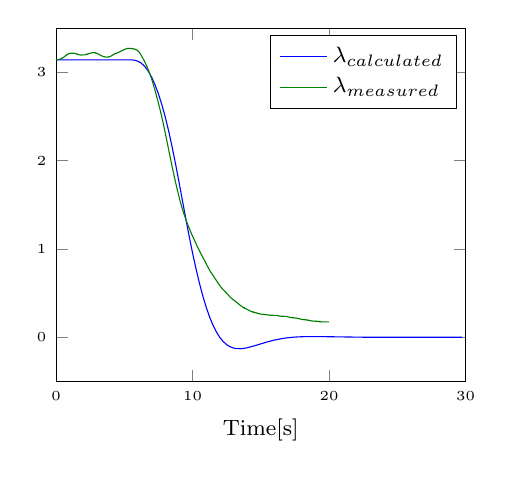
\begin{tikzpicture}

\begin{axis}[%
width = 5.2cm,
at={(0.758in,0.488in)},
scale only axis,
xmin=0,
xmax=30,
xlabel={\footnotesize{Time[s]}},
ymin=-0.5,
ymax=3.5,
ticklabel style = {font=\tiny},
axis background/.style={fill=white},
legend style={legend cell align=left, align=left, draw=black, font = \footnotesize}
]
\addplot [color=blue]
  table[row sep=crcr]{%
0	3.14159265358979\\
5.5	3.14159265358979\\
5.75	3.13784214136253\\
6	3.126215553458\\
6.25	3.10330930002996\\
6.5	3.06662741519118\\
6.75	3.01445392239416\\
7	2.94565627711757\\
7.25	2.85950776329355\\
7.5	2.75555158796515\\
7.75	2.63350511049028\\
8	2.4931956060321\\
8.25	2.3345185760643\\
8.5	2.15761746932766\\
8.75	1.96507893392501\\
9	1.76161316890801\\
9.5	1.3454468195671\\
9.75	1.14416130639108\\
10	0.953300334726706\\
10.25	0.775743116768965\\
10.5	0.613417116308511\\
10.75	0.467571581826093\\
11	0.338997628853846\\
11.25	0.228101632777872\\
11.5	0.134701135231747\\
11.75	0.0580618585324615\\
12	-0.00298121541176144\\
12.25	-0.0498875125411402\\
12.5	-0.0842868139618353\\
12.75	-0.107876607079184\\
13	-0.122342061837568\\
13.25	-0.129296679399445\\
13.5	-0.130240639346553\\
13.75	-0.126533838631495\\
14	-0.119380718351916\\
14.5	-0.0987485437619213\\
15.5	-0.05179257504345\\
16	-0.0320514641623504\\
16.5	-0.0165985935454387\\
17	-0.00551474553106601\\
17.5	0.00167407400259734\\
18	0.00571207248234273\\
18.75	0.00762976471574817\\
19.75	0.00611213632900842\\
22.5	0.000170594345526354\\
24.75	-0.000937229666892136\\
25.25	0\\
29.75	0\\
};
\addlegendentry{$\lambda_{\text{calculated}}$}

\addplot [color=black!50!green]
  table[row sep=crcr]{%
0	3.14159265358979\\
0.128	3.14235964398373\\
0.134	3.14312663437768\\
0.18	3.14389362477162\\
0.186	3.14466061516556\\
0.218	3.14542760555951\\
0.224	3.14619459595345\\
0.254000000000001	3.14696158634739\\
0.260000000000002	3.14772857674134\\
0.283999999999999	3.14849556713528\\
0.289999999999999	3.14926255752922\\
0.303999999999998	3.15002954792316\\
0.309999999999999	3.15079653831711\\
0.329999999999998	3.15156352871105\\
0.335999999999999	3.15233051910499\\
0.356000000000002	3.15309750949893\\
0.364000000000001	3.15463149028682\\
0.367999999999999	3.15386449989288\\
0.376000000000001	3.15539848068076\\
0.396000000000001	3.15616547107471\\
0.402000000000001	3.15769945186259\\
0.405999999999999	3.15693246146865\\
0.414000000000001	3.15846644225654\\
0.431999999999999	3.15923343265048\\
0.437999999999999	3.16000042304442\\
0.449999999999999	3.16076741343836\\
0.457999999999998	3.16230139422625\\
0.474	3.16306838462019\\
0.481999999999999	3.16460236540808\\
0.495999999999999	3.16536935580202\\
0.504000000000001	3.16690333658991\\
0.52	3.16767032698385\\
0.527999999999999	3.16920430777174\\
0.542000000000002	3.16997129816568\\
0.550000000000001	3.17150527895356\\
0.562000000000001	3.17227226934751\\
0.57	3.17380625013539\\
0.582000000000001	3.17457324052933\\
0.59	3.17610722131722\\
0.600000000000001	3.17687421171116\\
0.606000000000002	3.17764120210511\\
0.616	3.17840819249905\\
0.623999999999999	3.17994217328694\\
0.632000000000001	3.18070916368088\\
0.638000000000002	3.18147615407482\\
0.648	3.18224314446876\\
0.655999999999999	3.18377712525665\\
0.666	3.18454411565059\\
0.673999999999999	3.18607809643848\\
0.681999999999999	3.18684508683242\\
0.687999999999999	3.18761207722636\\
0.698	3.18837906762031\\
0.706	3.18991304840819\\
0.712	3.19068003880214\\
0.718	3.19144702919608\\
0.724	3.19221401959002\\
0.728000000000002	3.19298100998396\\
0.731999999999999	3.19221401959002\\
0.739999999999998	3.19374800037791\\
0.745999999999999	3.19451499077185\\
0.751999999999999	3.19528198116579\\
0.762	3.19604897155973\\
0.768000000000001	3.19681596195367\\
0.774000000000001	3.19758295234762\\
0.780000000000001	3.19834994274156\\
0.789999999999999	3.19911693313551\\
0.795999999999999	3.19988392352945\\
0.812000000000001	3.20065091392339\\
0.82	3.20218489471128\\
0.834	3.20295188510522\\
0.841999999999999	3.2044858658931\\
0.861999999999998	3.20525285628705\\
0.867999999999999	3.20601984668099\\
0.879999999999999	3.20678683707493\\
0.885999999999999	3.20755382746887\\
0.902000000000001	3.20832081786282\\
0.908000000000001	3.20908780825676\\
0.928000000000001	3.2098547986507\\
0.934000000000001	3.21062178904465\\
0.957999999999998	3.21138877943859\\
0.963999999999999	3.21215576983253\\
0.988	3.21292276022648\\
0.994	3.21368975062042\\
1.026	3.21445674101436\\
1.032	3.2152237314083\\
1.086	3.21599072180225\\
1.092	3.21675771219619\\
1.322	3.21599072180225\\
1.328	3.2152237314083\\
1.372	3.21445674101436\\
1.378	3.21368975062042\\
1.416	3.21292276022648\\
1.422	3.21215576983253\\
1.45	3.21138877943859\\
1.456	3.21062178904465\\
1.48	3.2098547986507\\
1.486	3.20908780825676\\
1.504	3.20832081786282\\
1.508	3.20755382746887\\
1.512	3.20832081786282\\
1.518	3.20755382746887\\
1.536	3.20678683707493\\
1.542	3.20601984668099\\
1.566	3.20525285628705\\
1.572	3.2044858658931\\
1.594	3.20371887549916\\
1.6	3.20295188510522\\
1.628	3.20218489471128\\
1.634	3.20141790431733\\
1.668	3.20065091392339\\
1.674	3.19988392352945\\
1.714	3.19911693313551\\
1.72	3.19834994274156\\
1.786	3.19758295234762\\
1.792	3.19681596195367\\
2.042	3.19758295234762\\
2.048	3.19834994274156\\
2.104	3.19911693313551\\
2.11	3.19988392352945\\
2.148	3.20065091392339\\
2.154	3.20141790431733\\
2.188	3.20218489471128\\
2.192	3.20295188510522\\
2.198	3.20218489471128\\
2.204	3.20295188510522\\
2.226	3.20371887549916\\
2.23	3.2044858658931\\
2.236	3.20371887549916\\
2.242	3.2044858658931\\
2.262	3.20525285628705\\
2.266	3.20601984668099\\
2.272	3.20525285628705\\
2.278	3.20601984668099\\
2.302	3.20678683707493\\
2.308	3.20755382746887\\
2.338	3.20832081786282\\
2.344	3.20908780825676\\
2.364	3.2098547986507\\
2.37	3.21062178904465\\
2.396	3.21138877943859\\
2.402	3.21215576983253\\
2.428	3.21292276022648\\
2.434	3.21368975062042\\
2.46	3.21445674101436\\
2.466	3.2152237314083\\
2.49	3.21599072180225\\
2.496	3.21675771219619\\
2.53	3.21752470259013\\
2.536	3.21829169298407\\
2.562	3.21905868337802\\
2.568	3.21982567377196\\
2.602	3.2205926641659\\
2.608	3.22135965455985\\
2.654	3.22212664495379\\
2.658	3.22212664495379\\
2.694	3.22289363534773\\
2.7	3.22366062574168\\
2.704	3.22366062574168\\
2.842	3.22289363534773\\
2.848	3.22212664495379\\
2.852	3.22289363534773\\
2.858	3.22135965455985\\
2.864	3.22212664495379\\
2.882	3.22135965455985\\
2.886	3.2205926641659\\
2.89	3.22135965455985\\
2.896	3.2205926641659\\
2.918	3.21982567377196\\
2.924	3.21905868337802\\
2.95	3.21829169298407\\
2.956	3.21752470259013\\
2.976	3.21675771219619\\
2.982	3.21599072180225\\
3	3.2152237314083\\
3.006	3.21445674101436\\
3.024	3.21368975062042\\
3.03	3.21292276022648\\
3.046	3.21215576983253\\
3.052	3.21138877943859\\
3.066	3.21062178904465\\
3.072	3.2098547986507\\
3.086	3.20908780825676\\
3.092	3.20832081786282\\
3.104	3.20755382746887\\
3.11	3.20678683707493\\
3.122	3.20601984668099\\
3.128	3.20525285628705\\
3.142	3.2044858658931\\
3.148	3.20371887549916\\
3.16	3.20295188510522\\
3.166	3.20218489471128\\
3.176	3.20141790431733\\
3.182	3.20065091392339\\
3.194	3.19988392352945\\
3.2	3.19911693313551\\
3.212	3.19834994274156\\
3.218	3.19758295234762\\
3.23	3.19681596195367\\
3.236	3.19604897155973\\
3.246	3.19528198116579\\
3.252	3.19451499077185\\
3.264	3.19374800037791\\
3.27	3.19298100998396\\
3.284	3.19221401959002\\
3.29	3.19144702919608\\
3.302	3.19068003880214\\
3.308	3.18991304840819\\
3.322	3.18914605801425\\
3.328	3.18837906762031\\
3.344	3.18761207722636\\
3.35	3.18684508683242\\
3.366	3.18607809643848\\
3.372	3.18531110604453\\
3.39	3.18454411565059\\
3.396	3.18377712525665\\
3.412	3.18301013486271\\
3.418	3.18224314446876\\
3.44	3.18147615407482\\
3.446	3.18070916368088\\
3.468	3.17994217328694\\
3.474	3.17917518289299\\
3.5	3.17840819249905\\
3.506	3.17764120210511\\
3.536	3.17687421171116\\
3.542	3.17610722131722\\
3.578	3.17534023092328\\
3.584	3.17457324052933\\
3.63	3.17380625013539\\
3.636	3.17303925974145\\
3.834	3.17380625013539\\
3.838	3.17457324052933\\
3.844	3.17380625013539\\
3.85	3.17457324052933\\
3.88	3.17534023092328\\
3.886	3.17610722131722\\
3.91	3.17687421171116\\
3.916	3.17764120210511\\
3.934	3.17840819249905\\
3.94	3.17917518289299\\
3.958	3.17994217328694\\
3.964	3.18070916368088\\
3.98	3.18147615407482\\
3.986	3.18224314446876\\
4	3.18301013486271\\
4.006	3.18377712525665\\
4.02	3.18454411565059\\
4.026	3.18531110604453\\
4.038	3.18607809643848\\
4.044	3.18684508683242\\
4.056	3.18761207722636\\
4.064	3.18914605801425\\
4.078	3.18991304840819\\
4.084	3.19068003880214\\
4.092	3.19144702919608\\
4.098	3.19221401959002\\
4.108	3.19298100998396\\
4.114	3.19374800037791\\
4.122	3.19451499077185\\
4.128	3.19528198116579\\
4.142	3.19604897155973\\
4.15	3.19758295234762\\
4.158	3.19834994274156\\
4.162	3.19911693313551\\
4.166	3.19911693313551\\
4.18	3.19988392352945\\
4.188	3.20141790431733\\
4.204	3.20218489471128\\
4.212	3.20371887549916\\
4.23	3.2044858658931\\
4.236	3.20525285628705\\
4.246	3.20601984668099\\
4.252	3.20678683707493\\
4.268	3.20755382746887\\
4.274	3.20832081786282\\
4.288	3.20908780825676\\
4.294	3.2098547986507\\
4.31	3.21062178904465\\
4.316	3.21138877943859\\
4.334	3.21215576983253\\
4.34	3.21292276022648\\
4.358	3.21368975062042\\
4.364	3.21445674101436\\
4.386	3.2152237314083\\
4.392	3.21599072180225\\
4.414	3.21675771219619\\
4.42	3.21752470259013\\
4.44	3.21829169298407\\
4.446	3.21905868337802\\
4.47	3.21982567377196\\
4.476	3.2205926641659\\
4.498	3.22135965455985\\
4.504	3.22212664495379\\
4.524	3.22289363534773\\
4.53	3.22366062574168\\
4.548	3.22442761613562\\
4.554	3.22519460652956\\
4.574	3.2259615969235\\
4.58	3.22672858731745\\
4.596	3.22749557771139\\
4.602	3.22826256810533\\
4.618	3.22902955849927\\
4.624	3.22979654889322\\
4.638	3.23056353928716\\
4.644	3.2313305296811\\
4.66	3.23209752007505\\
4.666	3.23286451046899\\
4.68	3.23363150086293\\
4.686	3.23439849125688\\
4.698	3.23516548165082\\
4.704	3.23593247204476\\
4.718	3.2366994624387\\
4.724	3.23746645283265\\
4.738	3.23823344322659\\
4.744	3.23900043362053\\
4.756	3.23976742401447\\
4.762	3.24053441440842\\
4.778	3.24130140480236\\
4.786	3.24283538559025\\
4.806	3.24360237598419\\
4.814	3.24513635677208\\
4.832	3.24590334716602\\
4.838	3.24667033755996\\
4.848	3.2474373279539\\
4.852	3.24820431834785\\
4.856	3.24820431834785\\
4.87	3.24897130874179\\
4.876	3.24973829913573\\
4.892	3.25050528952967\\
4.9	3.25203927031756\\
4.904	3.25203927031756\\
4.918	3.2528062607115\\
4.924	3.25357325110545\\
4.94	3.25434024149939\\
4.946	3.25510723189333\\
4.962	3.25587422228728\\
4.968	3.25664121268122\\
4.982	3.25740820307516\\
4.988	3.2581751934691\\
5.006	3.25894218386305\\
5.012	3.25970917425699\\
5.03	3.26047616465093\\
5.036	3.26124315504487\\
5.054	3.26201014543881\\
5.06	3.26277713583276\\
5.082	3.2635441262267\\
5.088	3.26431111662064\\
5.108	3.26507810701459\\
5.114	3.26584509740853\\
5.14	3.26661208780247\\
5.146	3.26737907819642\\
5.174	3.26814606859036\\
5.18	3.2689130589843\\
5.218	3.26968004937824\\
5.224	3.27044703977219\\
5.268	3.27121403016613\\
5.274	3.27198102056007\\
5.28	3.27121403016613\\
5.506	3.27044703977219\\
5.512	3.26968004937824\\
5.568	3.2689130589843\\
5.574	3.26814606859036\\
5.638	3.26737907819642\\
5.644	3.26661208780247\\
5.698	3.26584509740853\\
5.704	3.26507810701459\\
5.74	3.26431111662064\\
5.746	3.2635441262267\\
5.776	3.26277713583276\\
5.782	3.26201014543881\\
5.81	3.26124315504487\\
5.818	3.25970917425699\\
5.822	3.26047616465093\\
5.828	3.25970917425699\\
5.846	3.25894218386305\\
5.852	3.2581751934691\\
5.86	3.25740820307516\\
5.866	3.25664121268122\\
5.882	3.25587422228728\\
5.888	3.25510723189333\\
5.9	3.25434024149939\\
5.908	3.2528062607115\\
5.922	3.25203927031756\\
5.93	3.25050528952967\\
5.942	3.24973829913573\\
5.95	3.24820431834785\\
5.962	3.2474373279539\\
5.97	3.24590334716602\\
5.978	3.24513635677208\\
5.986	3.24360237598419\\
5.996	3.24283538559025\\
6.004	3.24130140480236\\
6.012	3.24053441440842\\
6.022	3.23823344322659\\
6.03	3.23746645283265\\
6.038	3.23593247204476\\
6.044	3.23516548165082\\
6.052	3.23363150086293\\
6.058	3.23286451046899\\
6.068	3.23056353928716\\
6.074	3.22979654889322\\
6.084	3.22749557771139\\
6.092	3.22672858731745\\
6.102	3.22442761613562\\
6.106	3.22366062574168\\
6.116	3.22135965455985\\
6.122	3.2205926641659\\
6.134	3.21752470259013\\
6.14	3.21675771219619\\
6.154	3.21292276022648\\
6.162	3.21215576983253\\
6.178	3.20755382746887\\
6.184	3.20678683707493\\
6.194	3.2044858658931\\
6.198	3.20371887549916\\
6.214	3.19911693313551\\
6.22	3.19834994274156\\
6.24	3.19221401959002\\
6.246	3.19144702919608\\
6.264	3.18607809643848\\
6.268	3.18531110604453\\
6.286	3.17994217328694\\
6.292	3.17917518289299\\
6.314	3.17227226934751\\
6.318	3.17150527895356\\
6.336	3.16613634619596\\
6.34	3.16536935580202\\
6.362	3.15846644225654\\
6.366	3.15769945186259\\
6.388	3.15079653831711\\
6.392	3.15002954792316\\
6.416	3.14235964398373\\
6.42	3.14159265358979\\
6.446	3.13315575925642\\
6.45	3.13238876886248\\
6.476	3.12395187452911\\
6.48	3.12318488413517\\
6.506	3.1147479898018\\
6.51	3.11398099940785\\
6.538	3.10477711468054\\
6.542	3.1040101242866\\
6.574	3.0932722587714\\
6.578	3.09250526837745\\
6.612	3.08100041246831\\
6.616	3.08023342207437\\
6.662	3.06412662380157\\
6.666	3.06335963340763\\
6.892	2.9751557381042\\
6.898	2.97208777652843\\
6.93	2.95828194943746\\
6.936	2.95521398786169\\
6.958	2.94524311274043\\
6.964	2.94217515116466\\
6.984	2.93297126643735\\
6.99	2.92990330486158\\
7.01	2.92069942013426\\
7.018	2.91609747777061\\
7.038	2.90689359304329\\
7.046	2.90229165067963\\
7.064	2.89385475634626\\
7.072	2.8892528139826\\
7.088	2.88158291004318\\
7.096	2.87698096767952\\
7.11	2.87007805413403\\
7.118	2.86547611177038\\
7.132	2.85857319822489\\
7.14	2.85397125586124\\
7.152	2.84783533270969\\
7.16	2.84323339034604\\
7.172	2.83709746719449\\
7.18	2.83249552483084\\
7.192	2.82635960167929\\
7.2	2.82175765931564\\
7.212	2.81562173616409\\
7.222	2.80948581301255\\
7.234	2.80334988986101\\
7.244	2.79721396670947\\
7.256	2.79107804355792\\
7.264	2.78647610119427\\
7.274	2.78110716843667\\
7.282	2.77650522607301\\
7.292	2.77113629331541\\
7.302	2.76500037016387\\
7.314	2.75886444701232\\
7.324	2.75272852386078\\
7.334	2.74735959110318\\
7.344	2.74122366795164\\
7.356	2.7350877448001\\
7.366	2.72895182164856\\
7.376	2.72358288889096\\
7.386	2.71744696573941\\
7.396	2.71207803298181\\
7.406	2.70594210983027\\
7.416	2.70057317707267\\
7.426	2.69443725392113\\
7.436	2.68906832116353\\
7.446	2.68293239801199\\
7.454	2.67833045564833\\
7.464	2.67219453249679\\
7.474	2.66682559973919\\
7.486	2.65915569579976\\
7.496	2.65378676304216\\
7.51	2.64458287831485\\
7.52	2.63921394555724\\
7.534	2.63001006082993\\
7.544	2.62464112807233\\
7.558	2.61543724334502\\
7.566	2.61083530098136\\
7.578	2.60316539704193\\
7.586	2.59856345467828\\
7.6	2.58935956995096\\
7.606	2.58552461798125\\
7.618	2.57785471404182\\
7.626	2.57325277167816\\
7.642	2.56251490616296\\
7.648	2.55867995419325\\
7.664	2.54794208867805\\
7.672	2.54334014631439\\
7.688	2.53260228079919\\
7.694	2.52876732882948\\
7.712	2.51649548252639\\
7.718	2.51266053055668\\
7.738	2.49885470346571\\
7.744	2.495019751496\\
7.766	2.47967994361714\\
7.772	2.47584499164742\\
7.792	2.46203916455645\\
7.798	2.45820421258674\\
7.828	2.43672848155634\\
7.834	2.43289352958663\\
7.872	2.40528187540469\\
7.878	2.40144692343497\\
7.926	2.3661653653136\\
7.932	2.36233041334389\\
8.02	2.29636923946481\\
8.024	2.29330127788903\\
8.17	2.18285466116127\\
8.174	2.18055368997944\\
8.18	2.17518475722184\\
8.186	2.17134980525212\\
8.402	2.00721386094836\\
8.408	2.00337890897865\\
8.414	1.99877696661499\\
8.5	1.9343497735238\\
8.506	1.93051482155408\\
8.512	1.92591287919042\\
8.56	1.89063132106905\\
8.564	1.88833034988722\\
8.57	1.88372840752357\\
8.61	1.85458277255374\\
8.616	1.85074782058403\\
8.648	1.82773810876574\\
8.654	1.82390315679603\\
8.684	1.80242742576563\\
8.69	1.79859247379591\\
8.712	1.78325266591706\\
8.718	1.77941771394734\\
8.742	1.7625439252806\\
8.748	1.75870897331089\\
8.766	1.7464371270078\\
8.772	1.74260217503809\\
8.792	1.72879634794712\\
8.798	1.7249613959774\\
8.816	1.71268954967432\\
8.822	1.7088545977046\\
8.838	1.6981167321894\\
8.846	1.69351478982575\\
8.866	1.67970896273478\\
8.874	1.67510702037112\\
8.892	1.66283517406804\\
8.9	1.65823323170438\\
8.918	1.64596138540129\\
8.926	1.64135944303764\\
8.94	1.63215555831032\\
8.948	1.62755361594667\\
8.962	1.61834973121935\\
8.97	1.61374778885569\\
8.984	1.60454390412838\\
8.992	1.59994196176472\\
9.004	1.59227205782529\\
9.014	1.5869031250677\\
9.028	1.57769924034038\\
9.038	1.57233030758278\\
9.052	1.56312642285547\\
9.062	1.55775749009787\\
9.07	1.55315554773421\\
9.08	1.54778661497661\\
9.09	1.54165069182507\\
9.1	1.53628175906747\\
9.11	1.53014583591593\\
9.122	1.52400991276438\\
9.132	1.51787398961284\\
9.144	1.5117380664613\\
9.154	1.50560214330976\\
9.168	1.49869922976427\\
9.178	1.49256330661273\\
9.192	1.48566039306724\\
9.2	1.48105845070359\\
9.214	1.4741555371581\\
9.222	1.46955359479444\\
9.238	1.46188369085502\\
9.246	1.45728174849136\\
9.262	1.44961184455193\\
9.27	1.44500990218827\\
9.286	1.43733999824885\\
9.292	1.43427203667308\\
9.31	1.4258351423397\\
9.316	1.42276718076393\\
9.334	1.41433028643056\\
9.34	1.41126232485479\\
9.358	1.40282543052142\\
9.364	1.39975746894565\\
9.386	1.38978659382439\\
9.392	1.38671863224862\\
9.418	1.37521377633948\\
9.424	1.37214581476371\\
9.45	1.36064095885456\\
9.456	1.35757299727879\\
9.488	1.34376717018782\\
9.494	1.34069920861205\\
9.532	1.32459241033925\\
9.538	1.32152444876348\\
9.584	1.30234968891491\\
9.59	1.29928172733914\\
9.654	1.27320405394508\\
9.66	1.27013609236931\\
9.908	1.17656326430829\\
9.912	1.17579627391434\\
9.916	1.17349530273252\\
9.92	1.17272831233857\\
9.97	1.15508753327789\\
9.974	1.15432054288394\\
10.024	1.13667976382326\\
10.028	1.13591277342932\\
10.074	1.11980597515652\\
10.078	1.11903898476258\\
10.124	1.10293218648978\\
10.128	1.10216519609583\\
10.178	1.08452441703515\\
10.182	1.08375742664121\\
10.228	1.0676506283684\\
10.232	1.06688363797446\\
10.278	1.05077683970167\\
10.282	1.05000984930772\\
10.326	1.03467004142886\\
10.33	1.03390305103492\\
10.368	1.02086421433789\\
10.372	1.02009722394395\\
10.406	1.00859236803481\\
10.41	1.00782537764087\\
10.44	0.997854502519608\\
10.444	0.997087512125667\\
10.472	0.987883627398354\\
10.476	0.987116637004409\\
10.5	0.979446733064982\\
10.504	0.978679742671041\\
10.53	0.970242848337669\\
10.534	0.969475857943724\\
10.556	0.962572944398239\\
10.56	0.961805954004298\\
10.586	0.953369059670926\\
10.592	0.952602069276985\\
10.62	0.943398184549668\\
10.624	0.942631194155727\\
10.642	0.937262261398129\\
10.646	0.936495271004183\\
10.668	0.929592357458699\\
10.672	0.928825367064757\\
10.694	0.921922453519272\\
10.698	0.921155463125327\\
10.716	0.915786530367729\\
10.72	0.915019539973784\\
10.74	0.908883616822241\\
10.744	0.908116626428299\\
10.766	0.901213712882814\\
10.77	0.900446722488873\\
10.792	0.893543808943384\\
10.796	0.892776818549443\\
10.816	0.8866408953979\\
10.82	0.885873905003958\\
10.842	0.878970991458473\\
10.846	0.878204001064528\\
10.87	0.870534097125102\\
10.874	0.86976710673116\\
10.896	0.862864193185672\\
10.9	0.86209720279173\\
10.926	0.853660308458359\\
10.93	0.852893318064417\\
10.954	0.845223414124987\\
10.958	0.844456423731046\\
10.984	0.836019529397674\\
10.988	0.835252539003733\\
11.012	0.827582635064303\\
11.016	0.826815644670361\\
11.04	0.819145740730931\\
11.044	0.81837875033699\\
11.068	0.81070884639756\\
11.072	0.809941856003618\\
11.094	0.803038942458134\\
11.098	0.802271952064192\\
11.12	0.795369038518704\\
11.124	0.794602048124762\\
11.144	0.788466124973219\\
11.148	0.787699134579277\\
11.166	0.782330201821676\\
11.17	0.781563211427734\\
11.188	0.776194278670136\\
11.192	0.775427288276191\\
11.21	0.770058355518593\\
11.214	0.769291365124648\\
11.23	0.764689422760991\\
11.234	0.76392243236705\\
11.25	0.759320490003393\\
11.254	0.758553499609448\\
11.268	0.754718547639737\\
11.272	0.753951557245792\\
11.288	0.749349614882135\\
11.292	0.748582624488193\\
11.306	0.744747672518479\\
11.31	0.743980682124537\\
11.322	0.740912720548764\\
11.326	0.740145730154822\\
11.34	0.736310778185107\\
11.344	0.735543787791165\\
11.358	0.731708835821451\\
11.364	0.730941845427509\\
11.38	0.726339903063852\\
11.386	0.725572912669907\\
11.402	0.720970970306251\\
11.408	0.720203979912309\\
11.422	0.716369027942594\\
11.426	0.715602037548653\\
11.438	0.712534075972879\\
11.444	0.711767085578938\\
11.458	0.707932133609223\\
11.464	0.707165143215281\\
11.48	0.702563200851625\\
11.486	0.70179621045768\\
11.5	0.697961258487968\\
11.506	0.697194268094023\\
11.518	0.694126306518253\\
11.522	0.693359316124308\\
11.534	0.690291354548538\\
11.54	0.689524364154597\\
11.554	0.685689412184882\\
11.56	0.68492242179094\\
11.572	0.681854460215167\\
11.576	0.681087469821225\\
11.588	0.678019508245452\\
11.594	0.67725251785151\\
11.608	0.673417565881795\\
11.614	0.672650575487854\\
11.626	0.669582613912084\\
11.63	0.668815623518139\\
11.642	0.665747661942369\\
11.646	0.664980671548424\\
11.658	0.661912709972654\\
11.664	0.661145719578712\\
11.676	0.658077758002939\\
11.68	0.657310767608998\\
11.694	0.653475815639283\\
11.7	0.652708825245341\\
11.712	0.649640863669568\\
11.716	0.648873873275626\\
11.728	0.645805911699856\\
11.732	0.645038921305911\\
11.746	0.6412039693362\\
11.752	0.640436978942255\\
11.766	0.63660202697254\\
11.77	0.635835036578598\\
11.782	0.632767075002828\\
11.788	0.632000084608883\\
11.802	0.628165132639172\\
11.806	0.627398142245227\\
11.818	0.624330180669457\\
11.824	0.623563190275512\\
11.838	0.6197282383058\\
11.842	0.618961247911855\\
11.854	0.615893286336085\\
11.86	0.615126295942144\\
11.874	0.611291343972429\\
11.878	0.610524353578484\\
11.89	0.607456392002714\\
11.896	0.606689401608772\\
11.908	0.603621440032999\\
11.912	0.602854449639057\\
11.924	0.599786488063287\\
11.93	0.599019497669342\\
11.942	0.595951536093573\\
11.948	0.595184545699627\\
11.96	0.592116584123858\\
11.966	0.591349593729916\\
11.978	0.588281632154143\\
11.984	0.587514641760201\\
11.996	0.584446680184428\\
12.002	0.583679689790486\\
12.014	0.580611728214716\\
12.02	0.579844737820771\\
12.03	0.577543766638943\\
12.036	0.576776776245001\\
12.046	0.574475805063173\\
12.052	0.573708814669232\\
12.062	0.5714078434874\\
12.068	0.570640853093458\\
12.078	0.56833988191163\\
12.084	0.567572891517688\\
12.094	0.56527192033586\\
12.1	0.564504929941915\\
12.11	0.562203958760087\\
12.116	0.561436968366145\\
12.124	0.559902987578258\\
12.13	0.559135997184317\\
12.14	0.556835026002489\\
12.146	0.556068035608543\\
12.156	0.553767064426715\\
12.164	0.553000074032774\\
12.172	0.551466093244887\\
12.178	0.550699102850945\\
12.186	0.549165122063059\\
12.19	0.548398131669117\\
12.198	0.54686415088123\\
12.204	0.546097160487289\\
12.212	0.544563179699402\\
12.216	0.543796189305461\\
12.222	0.543029198911515\\
12.226	0.542262208517574\\
12.232	0.541495218123632\\
12.238	0.540728227729687\\
12.246	0.539194246941804\\
12.25	0.538427256547859\\
12.258	0.536893275759976\\
12.266	0.536126285366031\\
12.274	0.534592304578148\\
12.28	0.533825314184202\\
12.288	0.532291333396319\\
12.294	0.531524343002374\\
12.302	0.529990362214487\\
12.31	0.529223371820546\\
12.318	0.527689391032659\\
12.324	0.526922400638718\\
12.332	0.525388419850831\\
12.338	0.524621429456889\\
12.346	0.523087448669003\\
12.352	0.522320458275061\\
12.36	0.520786477487174\\
12.368	0.520019487093233\\
12.376	0.518485506305346\\
12.38	0.517718515911405\\
12.388	0.516184535123518\\
12.396	0.515417544729576\\
12.406	0.513116573547748\\
12.414	0.512349583153803\\
12.422	0.51081560236592\\
12.428	0.510048611971975\\
12.436	0.508514631184092\\
12.442	0.507747640790146\\
12.45	0.506213660002263\\
12.456	0.505446669608318\\
12.464	0.503912688820431\\
12.47	0.50314569842649\\
12.48	0.500844727244662\\
12.488	0.50007773685072\\
12.496	0.498543756062833\\
12.502	0.497776765668892\\
12.51	0.496242784881005\\
12.516	0.495475794487064\\
12.526	0.493174823305235\\
12.534	0.49240783291129\\
12.542	0.490873852123404\\
12.546	0.490106861729462\\
12.554	0.488572880941575\\
12.56	0.487805890547634\\
12.568	0.486271909759747\\
12.572	0.485504919365805\\
12.578	0.484737928971864\\
12.582	0.483970938577919\\
12.59	0.482436957790036\\
12.596	0.48166996739609\\
12.604	0.480135986608207\\
12.61	0.479368996214262\\
12.62	0.477068025032434\\
12.628	0.476301034638492\\
12.638	0.474000063456664\\
12.646	0.473233073062719\\
12.656	0.470932101880891\\
12.664	0.470165111486949\\
12.672	0.468631130699062\\
12.678	0.467864140305121\\
12.686	0.466330159517234\\
12.692	0.465563169123293\\
12.7	0.464029188335406\\
12.706	0.463262197941464\\
12.716	0.460961226759636\\
12.724	0.460194236365691\\
12.732	0.458660255577808\\
12.738	0.457893265183863\\
12.746	0.45635928439598\\
12.752	0.455592294002034\\
12.76	0.454058313214151\\
12.768	0.453291322820206\\
12.776	0.451757342032323\\
12.782	0.450990351638378\\
12.79	0.449456370850491\\
12.798	0.44868938045655\\
12.806	0.447155399668663\\
12.814	0.446388409274721\\
12.822	0.444854428486835\\
12.828	0.444087438092893\\
12.836	0.442553457305007\\
12.846	0.441786466911065\\
12.854	0.440252486123178\\
12.862	0.439485495729237\\
12.87	0.43795151494135\\
12.878	0.437184524547408\\
12.886	0.435650543759522\\
12.896	0.43488355336558\\
12.904	0.433349572577693\\
12.914	0.432582582183752\\
12.922	0.431048601395865\\
12.934	0.430281611001924\\
12.942	0.428747630214037\\
12.95	0.427980639820095\\
12.956	0.42721364942615\\
12.962	0.426446659032209\\
12.968	0.425679668638267\\
12.976	0.424912678244322\\
12.982	0.42414568785038\\
12.988	0.423378697456435\\
12.994	0.422611707062494\\
13	0.421844716668552\\
13.006	0.421077726274607\\
13.018	0.420310735880665\\
13.026	0.418776755092779\\
13.034	0.418009764698837\\
13.04	0.417242774304896\\
13.046	0.416475783910951\\
13.052	0.415708793517009\\
13.058	0.414941803123067\\
13.064	0.414174812729122\\
13.072	0.413407822335181\\
13.078	0.412640831941239\\
13.09	0.411873841547294\\
13.098	0.410339860759407\\
13.106	0.409572870365466\\
13.112	0.408805879971524\\
13.118	0.408038889577579\\
13.124	0.407271899183637\\
13.132	0.406504908789696\\
13.138	0.405737918395751\\
13.146	0.404970928001809\\
13.154	0.403436947213923\\
13.166	0.402669956819981\\
13.174	0.401135976032094\\
13.184	0.400368985638153\\
13.192	0.398835004850266\\
13.202	0.398068014456324\\
13.208	0.397301024062379\\
13.214	0.396534033668438\\
13.22	0.395767043274496\\
13.226	0.395000052880551\\
13.232	0.394233062486609\\
13.238	0.393466072092668\\
13.244	0.392699081698723\\
13.25	0.391932091304781\\
13.256	0.39116510091084\\
13.264	0.390398110516895\\
13.272	0.388864129729011\\
13.282	0.388097139335066\\
13.288	0.387330148941125\\
13.294	0.386563158547183\\
13.3	0.385796168153238\\
13.306	0.385029177759296\\
13.312	0.384262187365355\\
13.318	0.38349519697141\\
13.324	0.382728206577468\\
13.33	0.381961216183523\\
13.336	0.381194225789582\\
13.342	0.38042723539564\\
13.348	0.379660245001695\\
13.354	0.378893254607753\\
13.36	0.378126264213812\\
13.366	0.377359273819867\\
13.372	0.376592283425925\\
13.378	0.375825293031983\\
13.384	0.375058302638038\\
13.39	0.374291312244097\\
13.396	0.373524321850155\\
13.402	0.37275733145621\\
13.408	0.371990341062268\\
13.416	0.371223350668327\\
13.424	0.36968936988044\\
13.436	0.368922379486495\\
13.444	0.367388398698612\\
13.454	0.366621408304667\\
13.462	0.365087427516784\\
13.472	0.364320437122839\\
13.478	0.363553446728897\\
13.486	0.362786456334955\\
13.494	0.361252475547069\\
13.506	0.360485485153127\\
13.514	0.35895150436524\\
13.524	0.358184513971299\\
13.53	0.357417523577354\\
13.538	0.356650533183412\\
13.544	0.355883542789467\\
13.552	0.355116552395526\\
13.56	0.353582571607639\\
13.574	0.352815581213697\\
13.58	0.352048590819756\\
13.59	0.351281600425811\\
13.598	0.349747619637927\\
13.608	0.348980629243982\\
13.614	0.348213638850041\\
13.624	0.347446648456099\\
13.63	0.346679658062154\\
13.64	0.345912667668212\\
13.646	0.345145677274271\\
13.656	0.344378686880326\\
13.662	0.343611696486384\\
13.67	0.342844706092439\\
13.676	0.342077715698498\\
13.69	0.341310725304556\\
13.698	0.339776744516669\\
13.716	0.339009754122728\\
13.724	0.337475773334841\\
13.742	0.336708782940899\\
13.748	0.335174802153013\\
13.752	0.335941792546954\\
13.76	0.334407811759071\\
13.778	0.333640821365126\\
13.786	0.332106840577243\\
13.79	0.332873830971185\\
13.798	0.331339850183298\\
13.814	0.330572859789356\\
13.822	0.32903887900147\\
13.838	0.328271888607528\\
13.844	0.327504898213583\\
13.86	0.326737907819641\\
13.868	0.325203927031755\\
13.886	0.324436936637813\\
13.892	0.323669946243871\\
13.904	0.322902955849926\\
13.91	0.322135965455985\\
13.924	0.321368975062043\\
13.932	0.319834994274157\\
13.95	0.319068003880215\\
13.956	0.31830101348627\\
13.972	0.317534023092328\\
13.98	0.316000042304442\\
13.998	0.3152330519105\\
14.004	0.314466061516555\\
14.012	0.313699071122613\\
14.018	0.312932080728672\\
14.034	0.312165090334727\\
14.04	0.311398099940785\\
14.056	0.310631109546843\\
14.064	0.309097128758957\\
14.084	0.308330138365015\\
14.09	0.30756314797107\\
14.1	0.306796157577129\\
14.106	0.306029167183187\\
14.12	0.305262176789242\\
14.126	0.3044951863953\\
14.142	0.303728196001359\\
14.148	0.302961205607414\\
14.16	0.302194215213472\\
14.166	0.301427224819527\\
14.182	0.300660234425585\\
14.188	0.299893244031644\\
14.202	0.299126253637699\\
14.208	0.298359263243757\\
14.224	0.297592272849815\\
14.23	0.29682528245587\\
14.246	0.296058292061929\\
14.252	0.295291301667987\\
14.268	0.294524311274042\\
14.274	0.293757320880101\\
14.294	0.292990330486159\\
14.3	0.292223340092214\\
14.316	0.291456349698272\\
14.322	0.290689359304331\\
14.344	0.289922368910386\\
14.35	0.289155378516444\\
14.376	0.288388388122499\\
14.382	0.287621397728557\\
14.404	0.286854407334616\\
14.41	0.286087416940671\\
14.43	0.285320426546729\\
14.436	0.284553436152787\\
14.44	0.285320426546729\\
14.446	0.283786445758842\\
14.452	0.284553436152787\\
14.458	0.283786445758842\\
14.48	0.283019455364901\\
14.484	0.283019455364901\\
14.502	0.282252464970959\\
14.508	0.281485474577014\\
14.544	0.280718484183073\\
14.55	0.279951493789131\\
14.58	0.279184503395186\\
14.586	0.278417513001244\\
14.614	0.277650522607303\\
14.62	0.276883532213358\\
14.65	0.276116541819416\\
14.656	0.275349551425471\\
14.66	0.276116541819416\\
14.666	0.275349551425471\\
14.688	0.274582561031529\\
14.694	0.273815570637588\\
14.724	0.273048580243643\\
14.73	0.272281589849701\\
14.762	0.27151459945576\\
14.768	0.270747609061814\\
14.798	0.269980618667873\\
14.804	0.269213628273931\\
14.834	0.268446637879986\\
14.84	0.267679647486045\\
14.872	0.266912657092103\\
14.878	0.266145666698158\\
14.912	0.265378676304216\\
14.918	0.264611685910275\\
14.954	0.26384469551633\\
14.96	0.263077705122388\\
15.002	0.262310714728443\\
15.008	0.261543724334501\\
15.066	0.26077673394056\\
15.072	0.260009743546615\\
15.144	0.259242753152673\\
15.148	0.258475762758732\\
15.154	0.259242753152673\\
15.16	0.258475762758732\\
15.164	0.259242753152673\\
15.17	0.258475762758732\\
15.292	0.257708772364786\\
15.298	0.256941781970845\\
15.302	0.257708772364786\\
15.308	0.256941781970845\\
15.386	0.256174791576903\\
15.392	0.255407801182958\\
15.398	0.256174791576903\\
15.404	0.255407801182958\\
15.46	0.254640810789017\\
15.466	0.253873820395075\\
15.528	0.25310683000113\\
15.534	0.252339839607188\\
15.592	0.251572849213247\\
15.598	0.250805858819302\\
15.662	0.25003886842536\\
15.668	0.249271878031418\\
15.788	0.248504887637473\\
15.792	0.247737897243532\\
15.798	0.248504887637473\\
16.104	0.247737897243532\\
16.108	0.246970906849587\\
16.114	0.247737897243532\\
16.12	0.246970906849587\\
16.188	0.246203916455645\\
16.194	0.245436926061704\\
16.236	0.244669935667758\\
16.242	0.243902945273817\\
16.292	0.243135954879875\\
16.298	0.24236896448593\\
16.336	0.241601974091989\\
16.342	0.240834983698047\\
16.394	0.240067993304102\\
16.4	0.23930100291016\\
16.472	0.238534012516219\\
16.478	0.237767022122274\\
16.636	0.237000031728332\\
16.64	0.237000031728332\\
16.796	0.23623304133439\\
16.8	0.23623304133439\\
16.85	0.235466050940445\\
16.856	0.234699060546504\\
16.906	0.233932070152559\\
16.912	0.233165079758617\\
16.956	0.232398089364676\\
16.962	0.23163109897073\\
17.002	0.230864108576789\\
17.008	0.230097118182847\\
17.04	0.229330127788902\\
17.046	0.228563137394961\\
17.076	0.227796147001019\\
17.082	0.227029156607074\\
17.114	0.226262166213132\\
17.12	0.225495175819191\\
17.16	0.224728185425246\\
17.166	0.223961195031304\\
17.208	0.223194204637363\\
17.214	0.222427214243417\\
17.274	0.221660223849476\\
17.28	0.220893233455531\\
17.364	0.220126243061589\\
17.368	0.219359252667648\\
17.374	0.220126243061589\\
17.38	0.219359252667648\\
17.386	0.220126243061589\\
17.392	0.219359252667648\\
17.5	0.218592262273702\\
17.504	0.218592262273702\\
17.564	0.217825271879761\\
17.568	0.217058281485819\\
17.574	0.217825271879761\\
17.58	0.217058281485819\\
17.632	0.216291291091874\\
17.638	0.215524300697933\\
17.678	0.214757310303991\\
17.682	0.213990319910046\\
17.688	0.214757310303991\\
17.694	0.213990319910046\\
17.726	0.213223329516104\\
17.732	0.212456339122163\\
17.764	0.211689348728218\\
17.77	0.210922358334276\\
17.8	0.210155367940335\\
17.806	0.209388377546389\\
17.836	0.208621387152448\\
17.842	0.207854396758503\\
17.874	0.207087406364561\\
17.88	0.20632041597062\\
17.912	0.205553425576674\\
17.918	0.204786435182733\\
17.956	0.204019444788791\\
17.962	0.203252454394846\\
18.006	0.202485464000905\\
18.012	0.201718473606963\\
18.072	0.200951483213018\\
18.078	0.200184492819076\\
18.156	0.199417502425135\\
18.162	0.19865051203119\\
18.168	0.199417502425135\\
18.174	0.19865051203119\\
18.244	0.197883521637248\\
18.248	0.197883521637248\\
18.318	0.197116531243307\\
18.324	0.196349540849361\\
18.378	0.19558255045542\\
18.382	0.194815560061475\\
18.388	0.19558255045542\\
18.394	0.194815560061475\\
18.438	0.194048569667533\\
18.444	0.193281579273592\\
18.448	0.194048569667533\\
18.454	0.193281579273592\\
18.486	0.192514588879646\\
18.492	0.191747598485705\\
18.534	0.190980608091763\\
18.54	0.190213617697818\\
18.572	0.189446627303877\\
18.578	0.188679636909935\\
18.62	0.18791264651599\\
18.626	0.187145656122048\\
18.67	0.186378665728107\\
18.676	0.185611675334162\\
18.728	0.18484468494022\\
18.734	0.184077694546279\\
18.802	0.183310704152333\\
18.808	0.182543713758392\\
18.95	0.181776723364447\\
18.954	0.181009732970505\\
18.96	0.181776723364447\\
18.966	0.181009732970505\\
18.972	0.181776723364447\\
18.978	0.181009732970505\\
18.982	0.181776723364447\\
18.988	0.181009732970505\\
19.11	0.180242742576564\\
19.114	0.180242742576564\\
19.17	0.179475752182618\\
19.174	0.178708761788677\\
19.18	0.179475752182618\\
19.186	0.178708761788677\\
19.256	0.177941771394735\\
19.26	0.17717478100079\\
19.266	0.177941771394735\\
19.272	0.17717478100079\\
19.328	0.176407790606849\\
19.334	0.175640800212907\\
19.422	0.174873809818962\\
19.428	0.17410681942502\\
19.99	0.17410681942502\\
};
\addlegendentry{$\lambda_{\text{measured}}$}

\end{axis}
\end{tikzpicture}%

        \phantomcaption
        \label{fig:4_best_travel}
    \end{subfigure}\vspace{-0.4cm}
    \caption{Comparison of best and worst travel result}
\end{figure}
